% Options for packages loaded elsewhere
% Options for packages loaded elsewhere
\PassOptionsToPackage{unicode}{hyperref}
\PassOptionsToPackage{hyphens}{url}
\PassOptionsToPackage{dvipsnames,svgnames,x11names}{xcolor}
%
\documentclass[
  english,
  11pt,
  letterpaper,
]{book}
\usepackage{xcolor}
\usepackage{amsmath,amssymb}
\setcounter{secnumdepth}{5}
\usepackage{iftex}
\ifPDFTeX
  \usepackage[T1]{fontenc}
  \usepackage[utf8]{inputenc}
  \usepackage{textcomp} % provide euro and other symbols
\else % if luatex or xetex
  \usepackage{unicode-math} % this also loads fontspec
  \defaultfontfeatures{Scale=MatchLowercase}
  \defaultfontfeatures[\rmfamily]{Ligatures=TeX,Scale=1}
\fi
\usepackage{lmodern}
\ifPDFTeX\else
  % xetex/luatex font selection
\fi
% Use upquote if available, for straight quotes in verbatim environments
\IfFileExists{upquote.sty}{\usepackage{upquote}}{}
\IfFileExists{microtype.sty}{% use microtype if available
  \usepackage[]{microtype}
  \UseMicrotypeSet[protrusion]{basicmath} % disable protrusion for tt fonts
}{}
\makeatletter
\@ifundefined{KOMAClassName}{% if non-KOMA class
  \IfFileExists{parskip.sty}{%
    \usepackage{parskip}
  }{% else
    \setlength{\parindent}{0pt}
    \setlength{\parskip}{6pt plus 2pt minus 1pt}}
}{% if KOMA class
  \KOMAoptions{parskip=half}}
\makeatother
% Make \paragraph and \subparagraph free-standing
\makeatletter
\ifx\paragraph\undefined\else
  \let\oldparagraph\paragraph
  \renewcommand{\paragraph}{
    \@ifstar
      \xxxParagraphStar
      \xxxParagraphNoStar
  }
  \newcommand{\xxxParagraphStar}[1]{\oldparagraph*{#1}\mbox{}}
  \newcommand{\xxxParagraphNoStar}[1]{\oldparagraph{#1}\mbox{}}
\fi
\ifx\subparagraph\undefined\else
  \let\oldsubparagraph\subparagraph
  \renewcommand{\subparagraph}{
    \@ifstar
      \xxxSubParagraphStar
      \xxxSubParagraphNoStar
  }
  \newcommand{\xxxSubParagraphStar}[1]{\oldsubparagraph*{#1}\mbox{}}
  \newcommand{\xxxSubParagraphNoStar}[1]{\oldsubparagraph{#1}\mbox{}}
\fi
\makeatother

\usepackage{color}
\usepackage{fancyvrb}
\newcommand{\VerbBar}{|}
\newcommand{\VERB}{\Verb[commandchars=\\\{\}]}
\DefineVerbatimEnvironment{Highlighting}{Verbatim}{commandchars=\\\{\}}
% Add ',fontsize=\small' for more characters per line
\usepackage{framed}
\definecolor{shadecolor}{RGB}{241,243,245}
\newenvironment{Shaded}{\begin{snugshade}}{\end{snugshade}}
\newcommand{\AlertTok}[1]{\textcolor[rgb]{0.68,0.00,0.00}{#1}}
\newcommand{\AnnotationTok}[1]{\textcolor[rgb]{0.37,0.37,0.37}{#1}}
\newcommand{\AttributeTok}[1]{\textcolor[rgb]{0.40,0.45,0.13}{#1}}
\newcommand{\BaseNTok}[1]{\textcolor[rgb]{0.68,0.00,0.00}{#1}}
\newcommand{\BuiltInTok}[1]{\textcolor[rgb]{0.00,0.23,0.31}{#1}}
\newcommand{\CharTok}[1]{\textcolor[rgb]{0.13,0.47,0.30}{#1}}
\newcommand{\CommentTok}[1]{\textcolor[rgb]{0.37,0.37,0.37}{#1}}
\newcommand{\CommentVarTok}[1]{\textcolor[rgb]{0.37,0.37,0.37}{\textit{#1}}}
\newcommand{\ConstantTok}[1]{\textcolor[rgb]{0.56,0.35,0.01}{#1}}
\newcommand{\ControlFlowTok}[1]{\textcolor[rgb]{0.00,0.23,0.31}{\textbf{#1}}}
\newcommand{\DataTypeTok}[1]{\textcolor[rgb]{0.68,0.00,0.00}{#1}}
\newcommand{\DecValTok}[1]{\textcolor[rgb]{0.68,0.00,0.00}{#1}}
\newcommand{\DocumentationTok}[1]{\textcolor[rgb]{0.37,0.37,0.37}{\textit{#1}}}
\newcommand{\ErrorTok}[1]{\textcolor[rgb]{0.68,0.00,0.00}{#1}}
\newcommand{\ExtensionTok}[1]{\textcolor[rgb]{0.00,0.23,0.31}{#1}}
\newcommand{\FloatTok}[1]{\textcolor[rgb]{0.68,0.00,0.00}{#1}}
\newcommand{\FunctionTok}[1]{\textcolor[rgb]{0.28,0.35,0.67}{#1}}
\newcommand{\ImportTok}[1]{\textcolor[rgb]{0.00,0.46,0.62}{#1}}
\newcommand{\InformationTok}[1]{\textcolor[rgb]{0.37,0.37,0.37}{#1}}
\newcommand{\KeywordTok}[1]{\textcolor[rgb]{0.00,0.23,0.31}{\textbf{#1}}}
\newcommand{\NormalTok}[1]{\textcolor[rgb]{0.00,0.23,0.31}{#1}}
\newcommand{\OperatorTok}[1]{\textcolor[rgb]{0.37,0.37,0.37}{#1}}
\newcommand{\OtherTok}[1]{\textcolor[rgb]{0.00,0.23,0.31}{#1}}
\newcommand{\PreprocessorTok}[1]{\textcolor[rgb]{0.68,0.00,0.00}{#1}}
\newcommand{\RegionMarkerTok}[1]{\textcolor[rgb]{0.00,0.23,0.31}{#1}}
\newcommand{\SpecialCharTok}[1]{\textcolor[rgb]{0.37,0.37,0.37}{#1}}
\newcommand{\SpecialStringTok}[1]{\textcolor[rgb]{0.13,0.47,0.30}{#1}}
\newcommand{\StringTok}[1]{\textcolor[rgb]{0.13,0.47,0.30}{#1}}
\newcommand{\VariableTok}[1]{\textcolor[rgb]{0.07,0.07,0.07}{#1}}
\newcommand{\VerbatimStringTok}[1]{\textcolor[rgb]{0.13,0.47,0.30}{#1}}
\newcommand{\WarningTok}[1]{\textcolor[rgb]{0.37,0.37,0.37}{\textit{#1}}}

\usepackage{longtable,booktabs,array}
\usepackage{calc} % for calculating minipage widths
% Correct order of tables after \paragraph or \subparagraph
\usepackage{etoolbox}
\makeatletter
\patchcmd\longtable{\par}{\if@noskipsec\mbox{}\fi\par}{}{}
\makeatother
% Allow footnotes in longtable head/foot
\IfFileExists{footnotehyper.sty}{\usepackage{footnotehyper}}{\usepackage{footnote}}
\makesavenoteenv{longtable}
\usepackage{graphicx}
\makeatletter
\newsavebox\pandoc@box
\newcommand*\pandocbounded[1]{% scales image to fit in text height/width
  \sbox\pandoc@box{#1}%
  \Gscale@div\@tempa{\textheight}{\dimexpr\ht\pandoc@box+\dp\pandoc@box\relax}%
  \Gscale@div\@tempb{\linewidth}{\wd\pandoc@box}%
  \ifdim\@tempb\p@<\@tempa\p@\let\@tempa\@tempb\fi% select the smaller of both
  \ifdim\@tempa\p@<\p@\scalebox{\@tempa}{\usebox\pandoc@box}%
  \else\usebox{\pandoc@box}%
  \fi%
}
% Set default figure placement to htbp
\def\fps@figure{htbp}
\makeatother



\ifLuaTeX
\usepackage[bidi=basic]{babel}
\else
\usepackage[bidi=default]{babel}
\fi
% get rid of language-specific shorthands (see #6817):
\let\LanguageShortHands\languageshorthands
\def\languageshorthands#1{}
\ifLuaTeX
  \usepackage[english]{selnolig} % disable illegal ligatures
\fi


\setlength{\emergencystretch}{3em} % prevent overfull lines

\providecommand{\tightlist}{%
  \setlength{\itemsep}{0pt}\setlength{\parskip}{0pt}}



 


% Force all included graphics to fit within page boundaries.
% Mermaid diagrams render to PNG and are included via \includegraphics;
% this ensures none of them overflow the text area.
\usepackage[export]{adjustbox}
\let\originalincludegraphics\includegraphics
\renewcommand{\includegraphics}[2][]{%
  \originalincludegraphics[max width=\linewidth,max height=0.85\textheight,keepaspectratio,#1]{#2}}
\makeatletter
\@ifpackageloaded{tcolorbox}{}{\usepackage[skins,breakable]{tcolorbox}}
\@ifpackageloaded{fontawesome5}{}{\usepackage{fontawesome5}}
\definecolor{quarto-callout-color}{HTML}{909090}
\definecolor{quarto-callout-note-color}{HTML}{0758E5}
\definecolor{quarto-callout-important-color}{HTML}{CC1914}
\definecolor{quarto-callout-warning-color}{HTML}{EB9113}
\definecolor{quarto-callout-tip-color}{HTML}{00A047}
\definecolor{quarto-callout-caution-color}{HTML}{FC5300}
\definecolor{quarto-callout-color-frame}{HTML}{acacac}
\definecolor{quarto-callout-note-color-frame}{HTML}{4582ec}
\definecolor{quarto-callout-important-color-frame}{HTML}{d9534f}
\definecolor{quarto-callout-warning-color-frame}{HTML}{f0ad4e}
\definecolor{quarto-callout-tip-color-frame}{HTML}{02b875}
\definecolor{quarto-callout-caution-color-frame}{HTML}{fd7e14}
\makeatother
\makeatletter
\@ifpackageloaded{bookmark}{}{\usepackage{bookmark}}
\makeatother
\makeatletter
\@ifpackageloaded{caption}{}{\usepackage{caption}}
\AtBeginDocument{%
\ifdefined\contentsname
  \renewcommand*\contentsname{Table of contents}
\else
  \newcommand\contentsname{Table of contents}
\fi
\ifdefined\listfigurename
  \renewcommand*\listfigurename{List of Figures}
\else
  \newcommand\listfigurename{List of Figures}
\fi
\ifdefined\listtablename
  \renewcommand*\listtablename{List of Tables}
\else
  \newcommand\listtablename{List of Tables}
\fi
\ifdefined\figurename
  \renewcommand*\figurename{Figure}
\else
  \newcommand\figurename{Figure}
\fi
\ifdefined\tablename
  \renewcommand*\tablename{Table}
\else
  \newcommand\tablename{Table}
\fi
}
\@ifpackageloaded{float}{}{\usepackage{float}}
\floatstyle{ruled}
\@ifundefined{c@chapter}{\newfloat{codelisting}{h}{lop}}{\newfloat{codelisting}{h}{lop}[chapter]}
\floatname{codelisting}{Listing}
\newcommand*\listoflistings{\listof{codelisting}{List of Listings}}
\makeatother
\makeatletter
\makeatother
\makeatletter
\@ifpackageloaded{caption}{}{\usepackage{caption}}
\@ifpackageloaded{subcaption}{}{\usepackage{subcaption}}
\makeatother
\usepackage{bookmark}
\IfFileExists{xurl.sty}{\usepackage{xurl}}{} % add URL line breaks if available
\urlstyle{same}
\hypersetup{
  pdftitle={Claude Code from Source},
  pdfauthor={Alejandro Balderas},
  pdflang={en},
  colorlinks=true,
  linkcolor={Maroon},
  filecolor={Maroon},
  citecolor={Blue},
  urlcolor={Blue},
  pdfcreator={LaTeX via pandoc}}


\title{Claude Code from Source}
\usepackage{etoolbox}
\makeatletter
\providecommand{\subtitle}[1]{% add subtitle to \maketitle
  \apptocmd{\@title}{\par {\large #1 \par}}{}{}
}
\makeatother
\subtitle{Architecture, Patterns \& Internals of Anthropic's AI Coding
Agent}
\author{Alejandro Balderas}
\date{2024-12-31}
\begin{document}
\frontmatter
\maketitle

\renewcommand*\contentsname{Table of contents}
{
\hypersetup{linkcolor=}
\setcounter{tocdepth}{1}
\tableofcontents
}

\mainmatter
\bookmarksetup{startatroot}

\chapter*{Preface}\label{preface}
\addcontentsline{toc}{chapter}{Preface}

\markboth{Preface}{Preface}

This book is the result of studying the architecture of Anthropic's
Claude Code and distilling the patterns, trade-offs, and design
decisions into a technical narrative that any engineer can learn from.

When Anthropic shipped Claude Code on npm, the \texttt{.js.map} source
maps contained a \texttt{sourcesContent} field with the full original
TypeScript. 36 AI agents analyzed nearly two thousand TypeScript files
across four phases --- exploration, analysis, writing, and review ---
producing this 18-chapter book in approximately six hours.

\textbf{What You Will Find Here}

Each chapter has layered depth: a narrative flow for technical leaders,
deep-dive sections for implementers, and an \emph{Apply This} closing
that extracts transferable patterns you can use in your own systems.

\textbf{The 10 Patterns That Make It Work}

If you read nothing else:

\begin{enumerate}
\def\labelenumi{\arabic{enumi}.}
\tightlist
\item
  \textbf{AsyncGenerator as agent loop} --- yields Messages, typed
  Terminal return, natural backpressure and cancellation
\item
  \textbf{Speculative tool execution} --- start read-only tools during
  model streaming, before the response completes
\item
  \textbf{Concurrent-safe batching} --- partition tools by safety, run
  reads in parallel, serialize writes
\item
  \textbf{Fork agents for cache sharing} --- parallel children share
  byte-identical prompt prefixes, saving \textasciitilde95\% input
  tokens
\item
  \textbf{4-layer context compression} --- snip, microcompact, collapse,
  autocompact --- each lighter than the next
\item
  \textbf{File-based memory with LLM recall} --- Sonnet side-query
  selects relevant memories, not keyword matching
\item
  \textbf{Two-phase skill loading} --- frontmatter only at startup, full
  content on invocation
\item
  \textbf{Sticky latches for cache stability} --- once a beta header is
  sent, never unset mid-session
\item
  \textbf{Slot reservation} --- 8K default output cap, escalate to 64K
  on hit (saves context in 99\% of requests)
\item
  \textbf{Hook config snapshot} --- freeze at startup to prevent runtime
  injection attacks
\end{enumerate}

\begin{tcolorbox}[enhanced jigsaw, opacitybacktitle=0.6, coltitle=black, arc=.35mm, colframe=quarto-callout-note-color-frame, colback=white, leftrule=.75mm, colbacktitle=quarto-callout-note-color!10!white, breakable, left=2mm, toptitle=1mm, opacityback=0, toprule=.15mm, bottomtitle=1mm, title=\textcolor{quarto-callout-note-color}{\faInfo}\hspace{0.5em}{Note}, titlerule=0mm, rightrule=.15mm, bottomrule=.15mm]

This book does not contain any source code from Claude Code. All code
blocks are original pseudocode using different variable names, written
to illustrate architectural patterns. No proprietary prompt text,
internal constants, or exact function implementations are included. This
project exists purely for educational purposes.

\end{tcolorbox}

\part{Part I: Foundations}

\chapter{Chapter 1: The Architecture of an AI
Agent}\label{chapter-1-the-architecture-of-an-ai-agent}

\section{What You're Looking At}\label{what-youre-looking-at}

A traditional CLI is a function. It takes arguments, does work, and
exits. \texttt{grep} does not decide to also run \texttt{sed}.
\texttt{curl} does not open a file and patch it based on what it
downloaded. The contract is simple: one command, one action,
deterministic output.

An agentic CLI breaks every part of that contract. It takes a natural
language prompt, decides what tools to use, executes them in whatever
order the situation demands, evaluates the results, and loops until the
task is done or the user stops it. The ``program'' is not a fixed
sequence of instructions -- it is a loop around a language model that
generates its own instruction sequence at runtime. The tool calls are
the side effects. The model's reasoning is the control flow.

Claude Code is Anthropic's production implementation of this idea: a
TypeScript monolith of nearly two thousand files that turns a terminal
into a full development environment powered by Claude. It shipped to
hundreds of thousands of developers, which means every architectural
decision carries real-world consequences. This chapter gives you the
mental model. Six abstractions define the entire system. A single data
flow connects them. Once you internalize the golden path from keystroke
to final output, every subsequent chapter is a zoom into one segment of
that path.

What follows is a retrospective decomposition -- these six abstractions
were not designed upfront on a whiteboard. They emerged from the
pressures of shipping a production agent to a large user base.
Understanding them as they are, not as they were planned, sets the right
expectations for the rest of the book.

\begin{center}\rule{0.5\linewidth}{0.5pt}\end{center}

\section{The Six Key Abstractions}\label{the-six-key-abstractions}

Claude Code is built on six core abstractions. Everything else -- the
400+ utility files, the forked terminal renderer, the vim emulation, the
cost tracker -- exists to support these six.

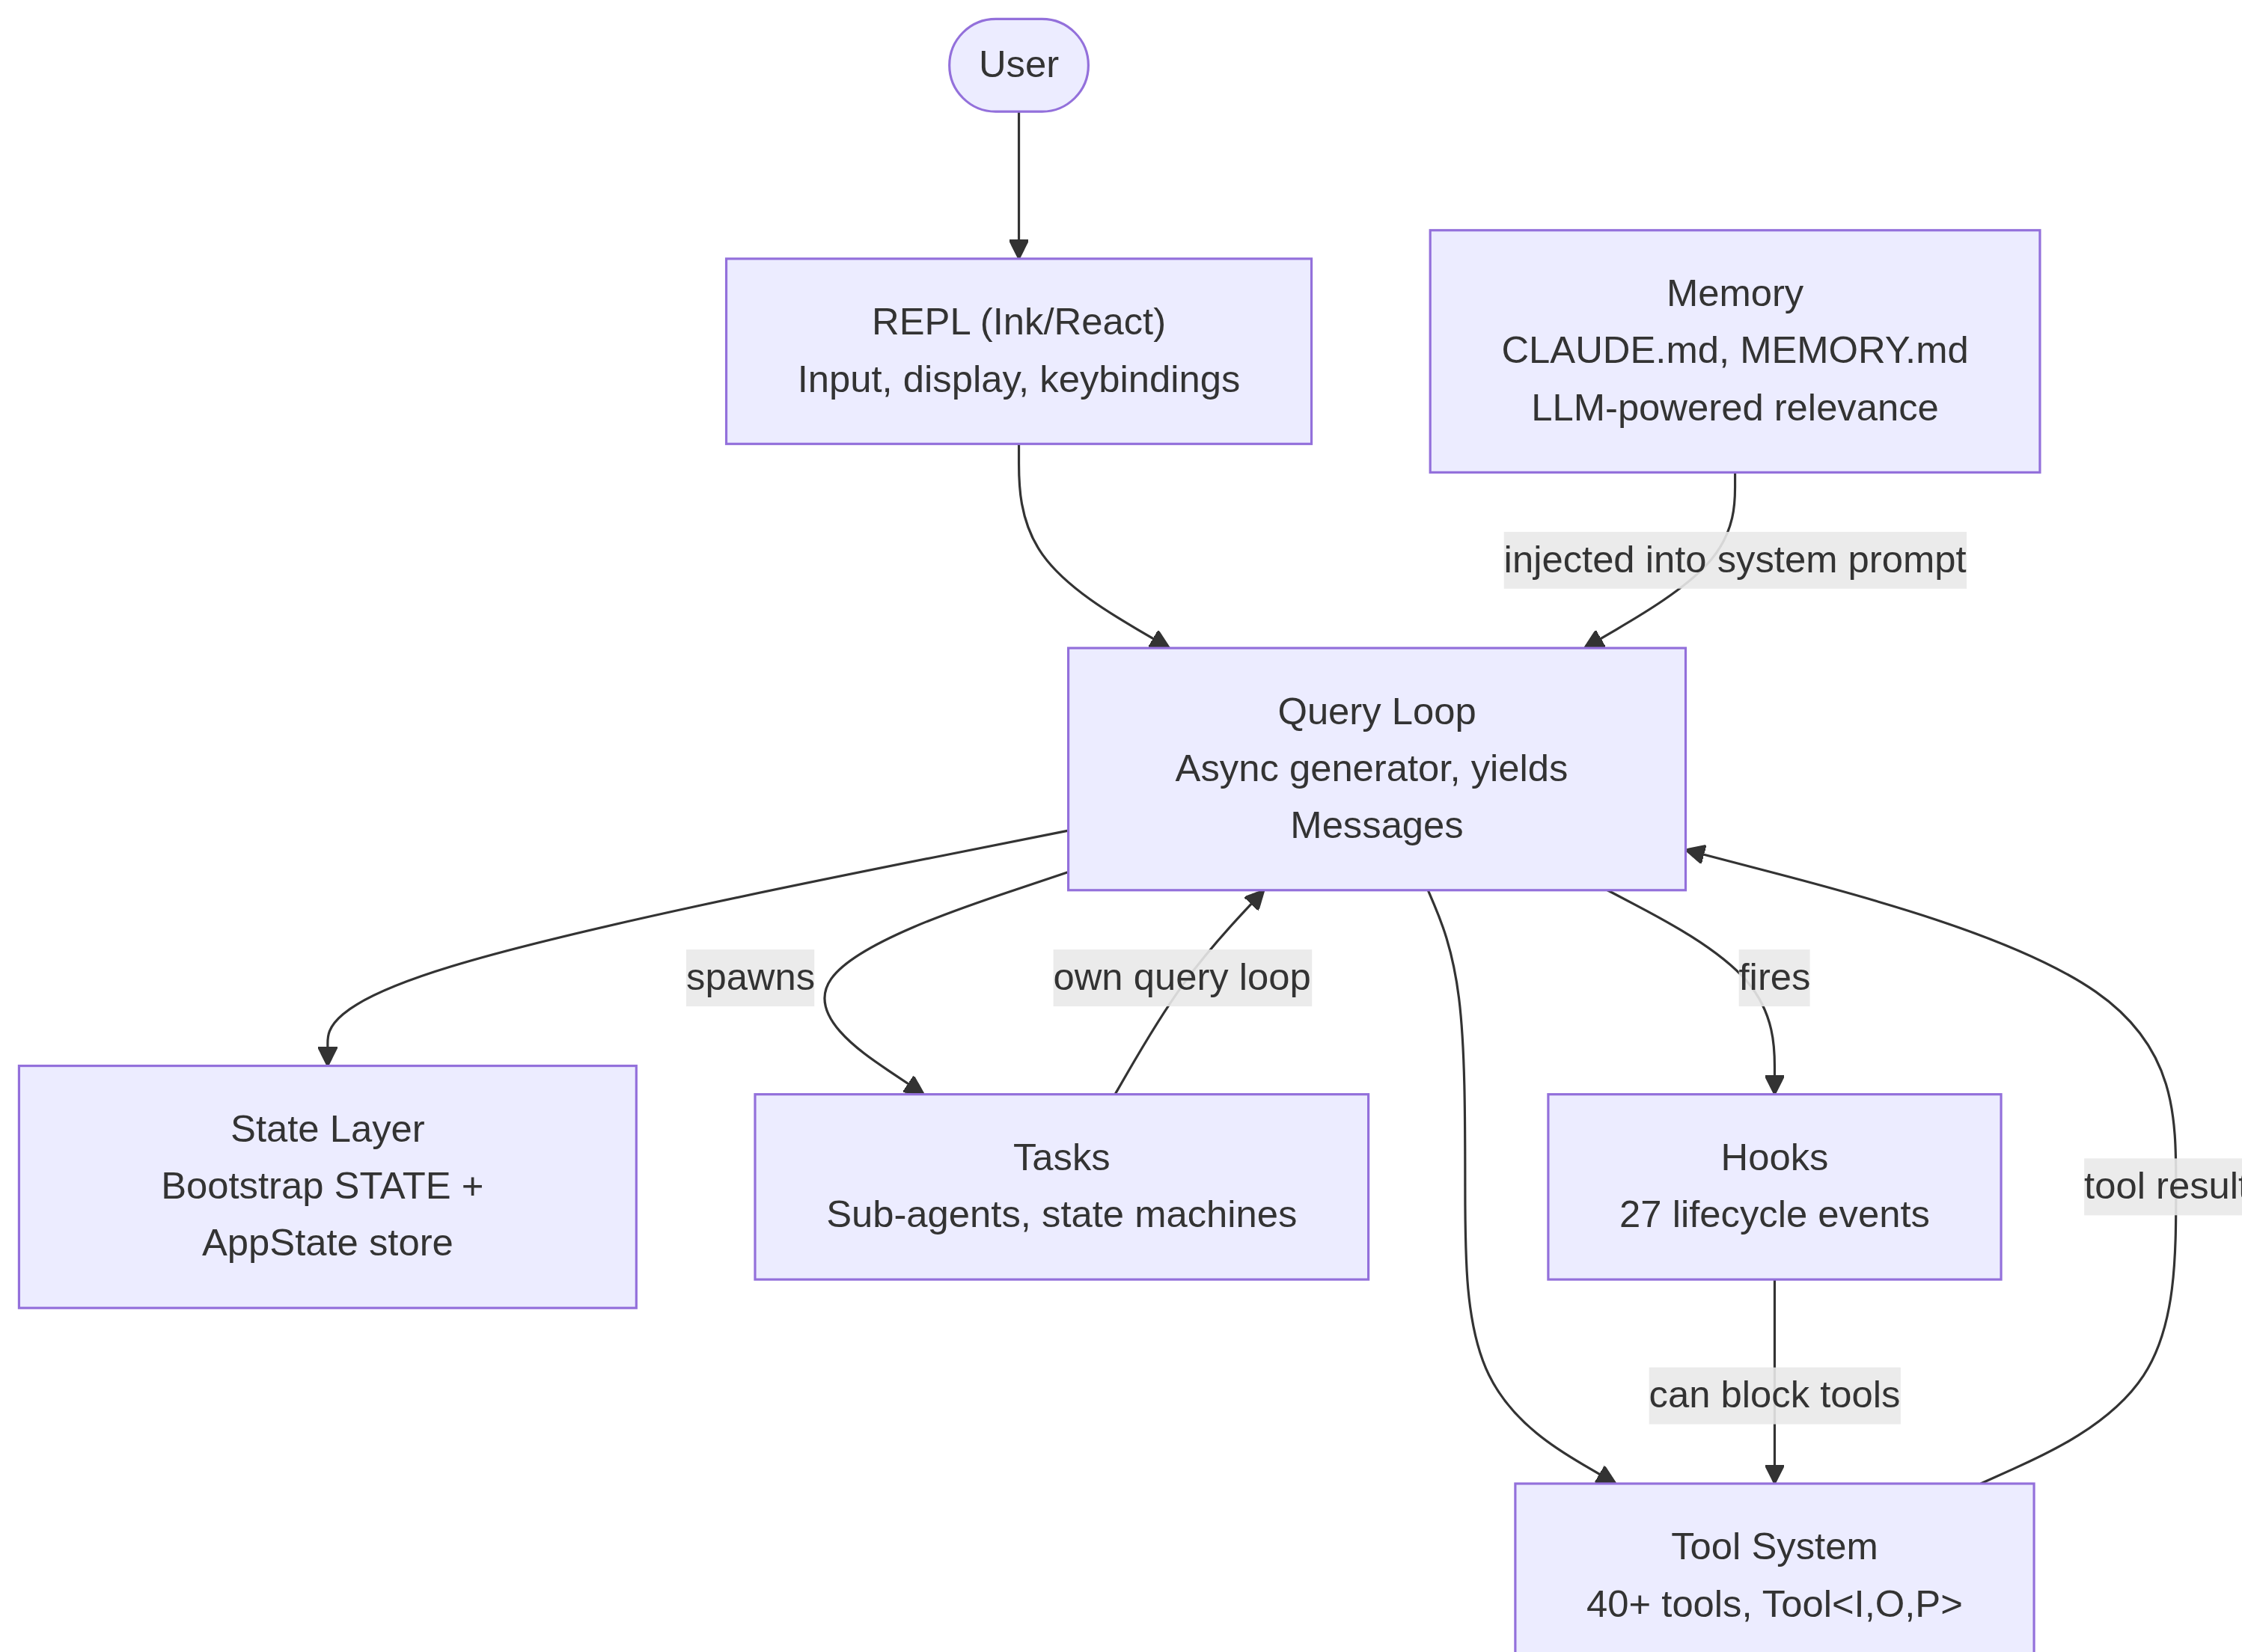
\includegraphics[width=10.03in,height=7.41in]{book/ch01-architecture_files/figure-latex/mermaid-figure-1.png}

Here is what each one does and why it exists.

\textbf{1. The Query Loop} (\texttt{query.ts}, \textasciitilde1,700
lines). An async generator that is the heartbeat of the entire system.
It streams a model response, collects tool calls, executes them, appends
results to the message history, and loops. Every interaction -- REPL,
SDK, sub-agent, headless \texttt{-\/-print} -- flows through this single
function. It yields \texttt{Message} objects that the UI consumes. Its
return type is a discriminated union called \texttt{Terminal} that
encodes exactly why the loop stopped: normal completion, user abort,
token budget exhaustion, stop hook intervention, max turns, or
unrecoverable error. The generator pattern -- rather than callbacks or
event emitters -- gives natural backpressure, clean cancellation, and
typed terminal states. Chapter 5 covers the loop's internals in full.

\textbf{2. The Tool System} (\texttt{Tool.ts}, \texttt{tools.ts},
\texttt{services/tools/}). A tool is anything the agent can do in the
world: read a file, run a shell command, edit code, search the web. That
simplicity of purpose hides significant machinery. Each tool implements
a rich interface covering identity, schema, execution, permissions, and
rendering. Tools are not just functions -- they carry their own
permission logic, concurrency declarations, progress reporting, and UI
rendering. The system partitions tool calls into concurrent and serial
batches, and a streaming executor starts concurrency-safe tools before
the model even finishes its response. Chapter 6 covers the full tool
interface and execution pipeline.

\textbf{3. Tasks} (\texttt{Task.ts}, \texttt{tasks/}). Tasks are
background work units -- primarily sub-agents. They follow a state
machine:
\texttt{pending\ -\textgreater{}\ running\ -\textgreater{}\ completed\ \textbar{}\ failed\ \textbar{}\ killed}.
The \texttt{AgentTool} spawns a new \texttt{query()} generator with its
own message history, tool set, and permission mode. Tasks give Claude
Code its recursive capability: an agent can delegate to sub-agents,
which can delegate further.

\textbf{4. State} (two layers). The system maintains state at two
levels. A mutable singleton (\texttt{STATE}) holds \textasciitilde80
fields of session-level infrastructure: working directory, model
configuration, cost tracking, telemetry counters, session ID. It is set
once at startup and mutated directly -- no reactivity. A minimal
reactive store (34 lines, Zustand-shaped) drives the UI: messages, input
mode, tool approvals, progress indicators. The separation is
intentional: infrastructure state changes rarely and does not need to
trigger re-renders; UI state changes constantly and must. Chapter 3
covers the two-tier architecture in depth.

\textbf{5. Memory} (\texttt{memdir/}). The agent's persistent context
across sessions. Three tiers: project-level (\texttt{CLAUDE.md} files in
the repo), user-level (\texttt{\textasciitilde{}/.claude/MEMORY.md}),
and team-level (shared via symlinks). At session start, the system scans
for all memory files, parses frontmatter, and an LLM selects which
memories are relevant to the current conversation. Memory is how Claude
Code ``remembers'' your codebase conventions, architectural decisions,
and debugging history.

\textbf{6. Hooks} (\texttt{hooks/}, \texttt{utils/hooks/}). User-defined
lifecycle interceptors that fire at 27 distinct events across 4
execution types: shell commands, single-shot LLM prompts, multi-turn
agent conversations, and HTTP webhooks. Hooks can block tool execution,
modify inputs, inject additional context, or short-circuit the entire
query loop. The permission system itself is partially implemented
through hooks -- \texttt{PreToolUse} hooks can deny tool calls before
the interactive permission prompt ever fires.

\begin{center}\rule{0.5\linewidth}{0.5pt}\end{center}

\section{The Golden Path: From Keystroke to
Output}\label{the-golden-path-from-keystroke-to-output}

Trace a single request through the system. The user types ``add error
handling to the login function'' and presses Enter.

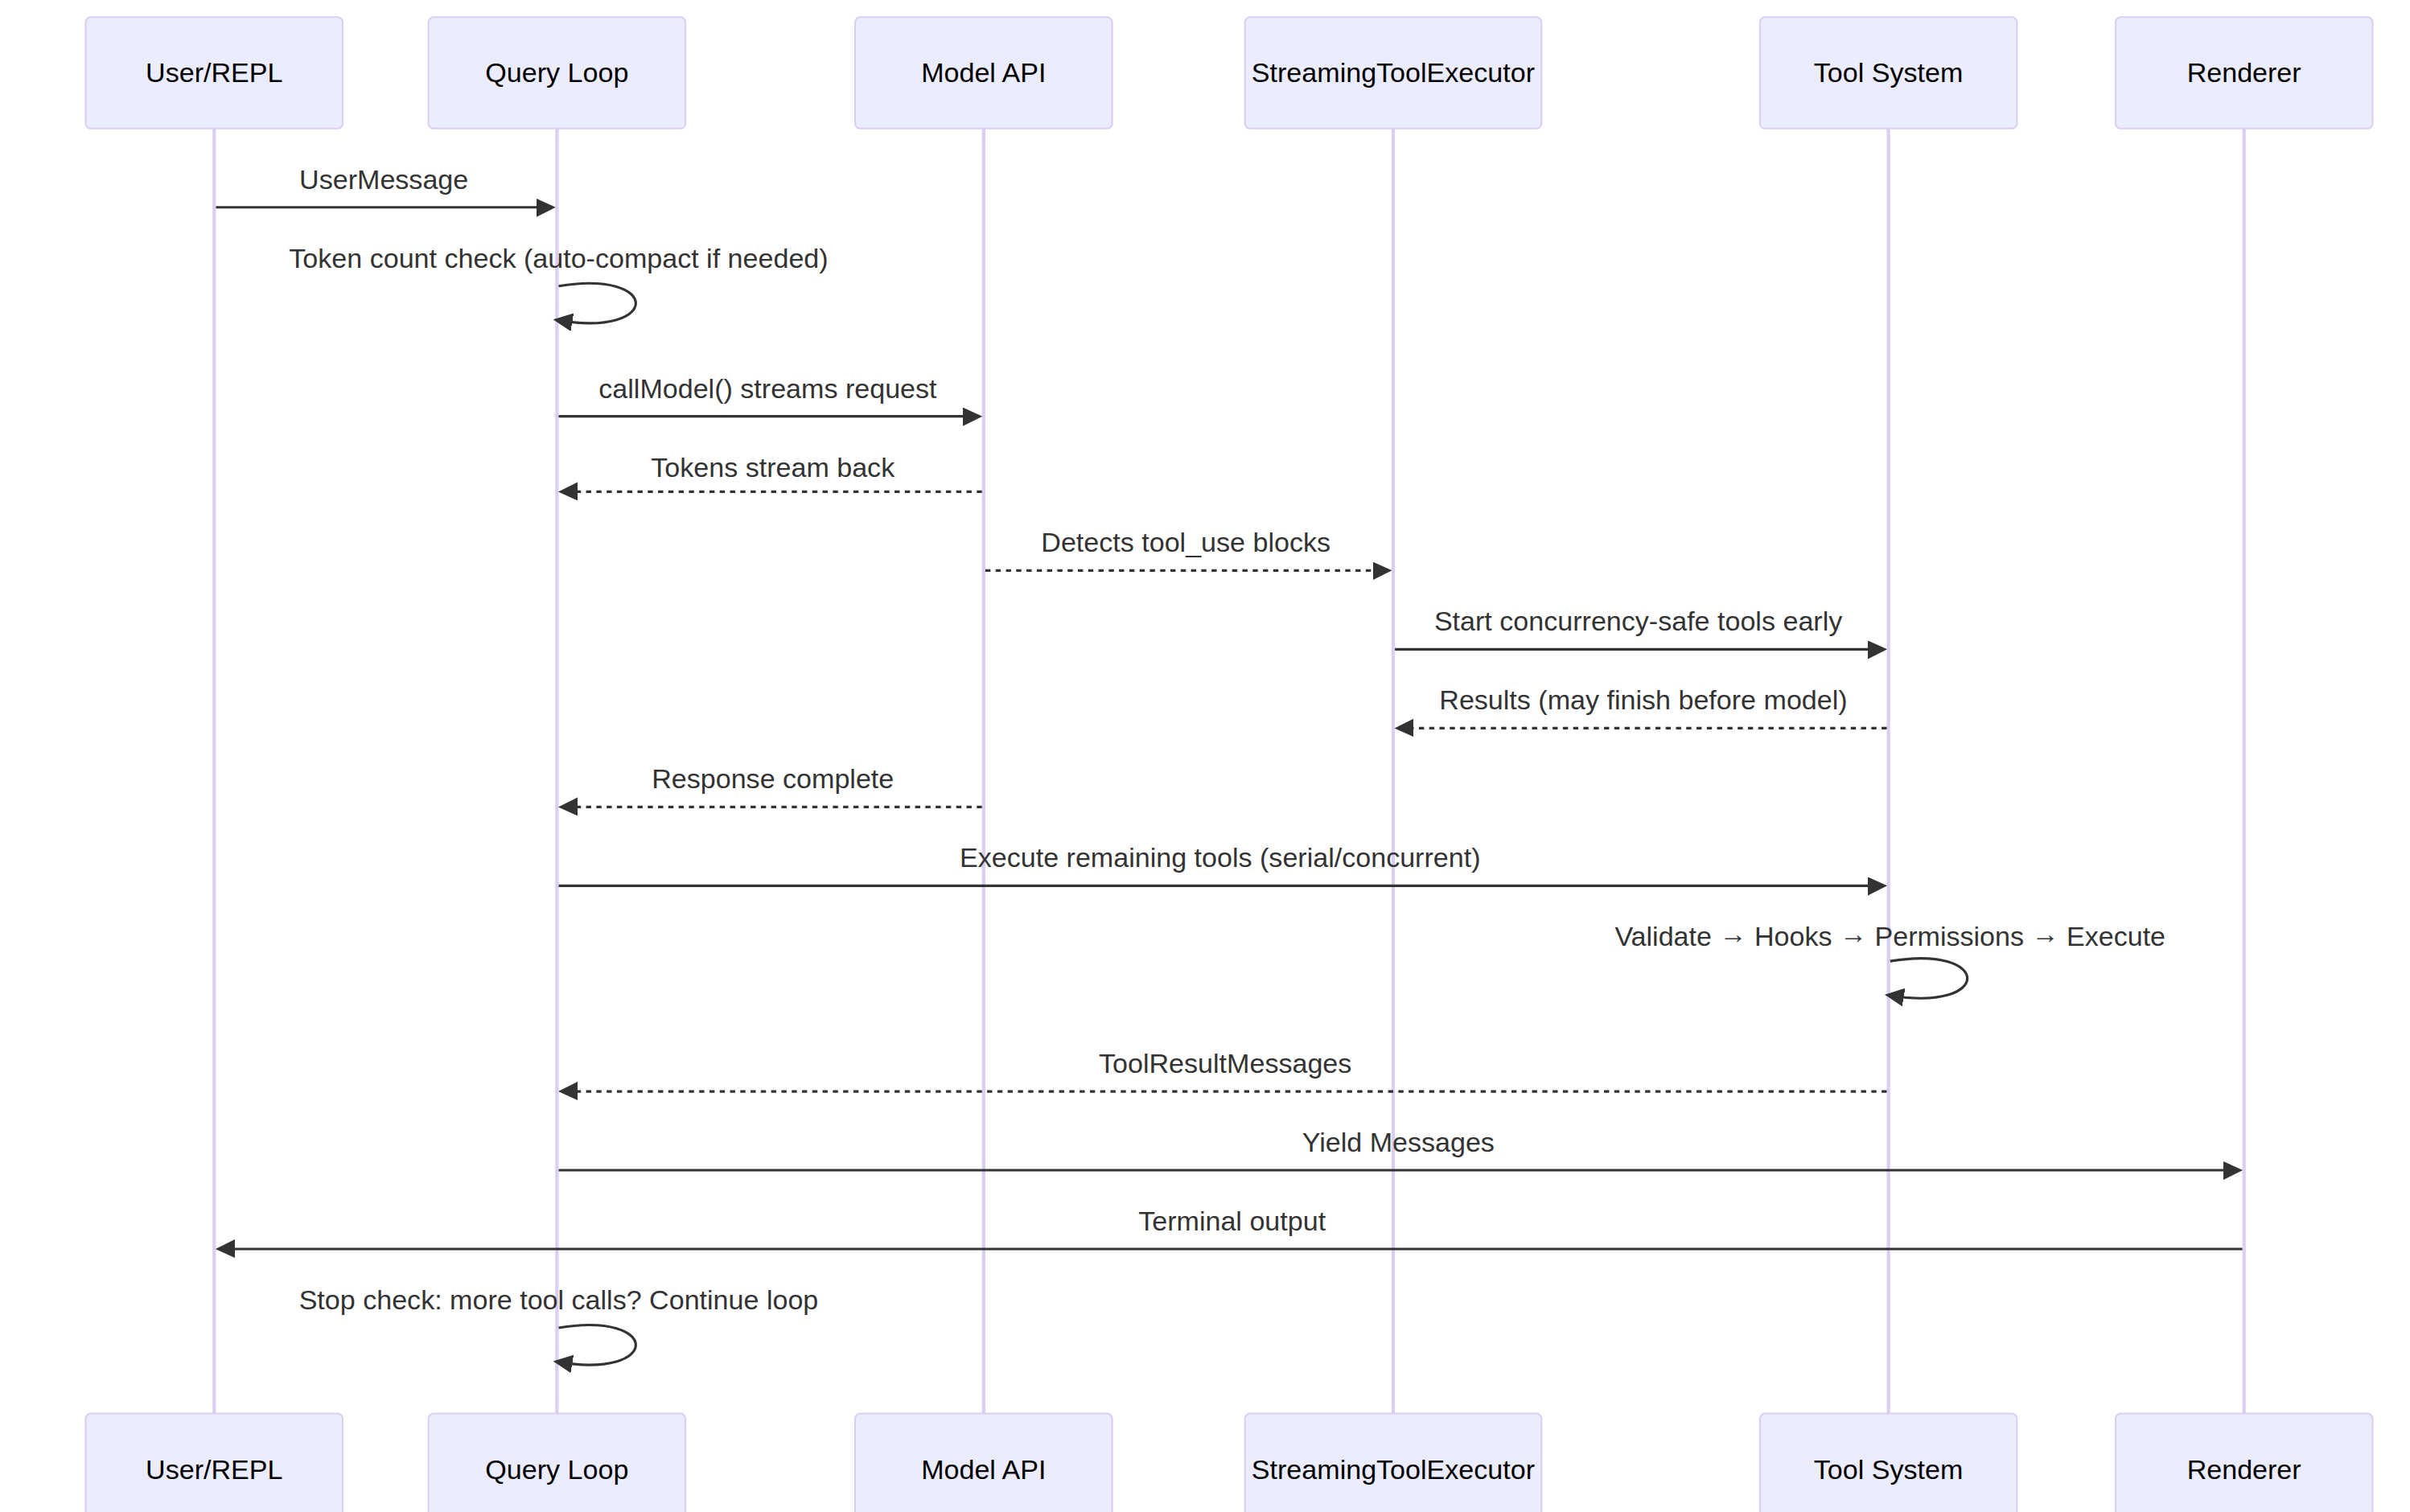
\includegraphics[width=14.94in,height=9.39in]{book/ch01-architecture_files/figure-latex/mermaid-figure-5.png}

Three things to notice about this flow.

First, the query loop is a generator, not a callback chain. The REPL
pulls messages from it via \texttt{for\ await}, which means backpressure
is natural -- if the UI cannot keep up, the generator pauses. This is a
deliberate choice over event emitters or observable streams.

Second, tool execution overlaps with model streaming. The
\texttt{StreamingToolExecutor} does not wait for the model to finish
before starting concurrency-safe tools. A \texttt{Read} call can
complete and return its results while the model is still generating the
rest of its response. This is speculative execution -- if the model's
final output invalidates the tool call (rare but possible), the result
is discarded.

Third, the entire loop is re-entrant. When the model makes tool calls,
the results are appended to the message history, and the loop calls the
model again with the updated context. There is no separate ``tool result
handling'' phase -- it is all one loop. The model decides when it is
done by simply not making any more tool calls.

\begin{center}\rule{0.5\linewidth}{0.5pt}\end{center}

\section{The Permission System}\label{the-permission-system}

Claude Code runs arbitrary shell commands on your machine. It edits your
files. It can spawn sub-processes, make network requests, and modify
your git history. Without a permission system, this is a security
catastrophe.

The system defines seven permission modes, ordered from most to least
permissive:

\begin{longtable}[]{@{}
  >{\raggedright\arraybackslash}p{(\linewidth - 2\tabcolsep) * \real{0.3750}}
  >{\raggedright\arraybackslash}p{(\linewidth - 2\tabcolsep) * \real{0.6250}}@{}}
\toprule\noalign{}
\begin{minipage}[b]{\linewidth}\raggedright
Mode
\end{minipage} & \begin{minipage}[b]{\linewidth}\raggedright
Behavior
\end{minipage} \\
\midrule\noalign{}
\endhead
\bottomrule\noalign{}
\endlastfoot
\texttt{bypassPermissions} & Everything allowed. No checks.
Internal/testing only. \\
\texttt{dontAsk} & All allowed, but still logged. No user prompts. \\
\texttt{auto} & Transcript classifier (LLM) decides allow/deny. \\
\texttt{acceptEdits} & File edits auto-approved; all other mutations
prompt. \\
\texttt{default} & Standard interactive mode. User approves each
action. \\
\texttt{plan} & Read-only. All mutations blocked. \\
\texttt{bubble} & Escalate decision to parent agent (sub-agent mode). \\
\end{longtable}

When a tool call needs permission, the resolution follows a strict
chain:

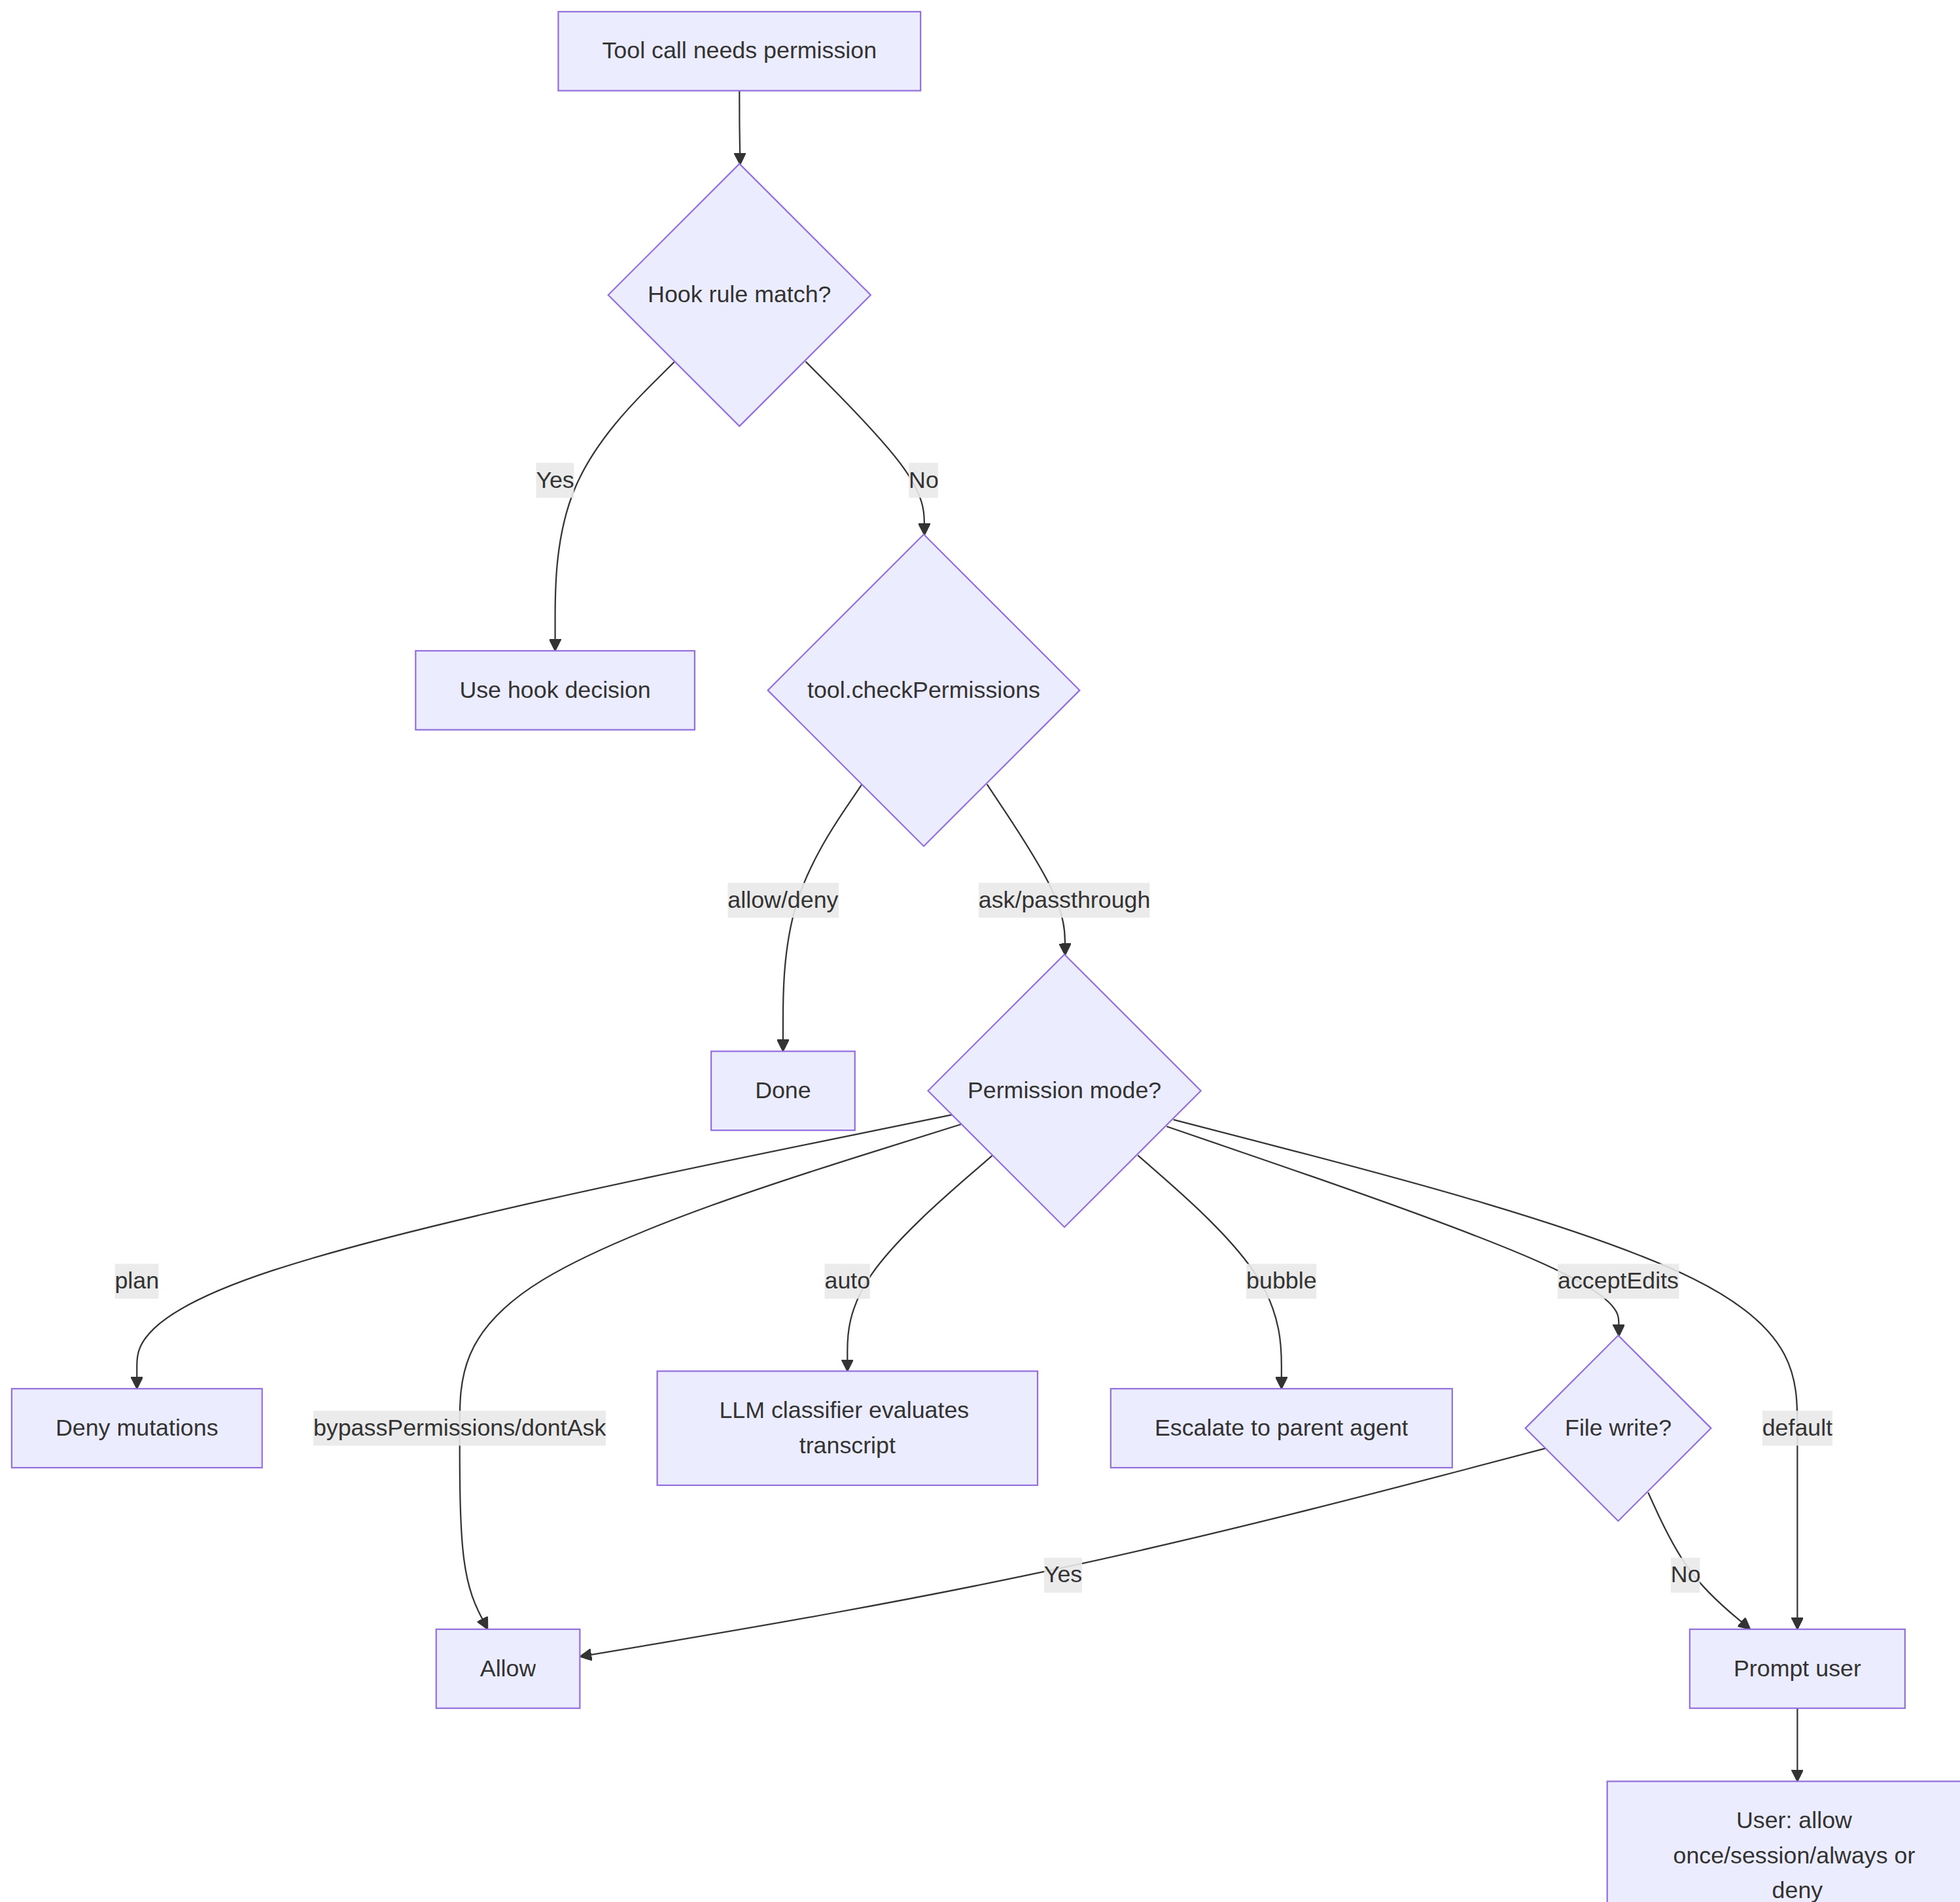
\includegraphics[width=14.24in,height=13.83in]{book/ch01-architecture_files/figure-latex/mermaid-figure-4.png}

The \texttt{auto} mode deserves special attention. It runs a separate,
lightweight LLM call that classifies the tool invocation against the
conversation transcript. The classifier sees a compact representation of
the tool input and decides whether the action is consistent with what
the user asked for. This is the mode that lets Claude Code work
semi-autonomously -- approving routine operations while flagging
anything that looks like it deviates from the user's intent.

Sub-agents default to \texttt{bubble} mode, which means they cannot
approve their own dangerous actions. Permission requests propagate up to
the parent agent or ultimately to the user. This prevents a sub-agent
from silently running destructive commands that the user never saw.

\begin{center}\rule{0.5\linewidth}{0.5pt}\end{center}

\section{Multi-Provider Architecture}\label{multi-provider-architecture}

Claude Code talks to Claude through four different infrastructure paths,
all transparent to the rest of the system.

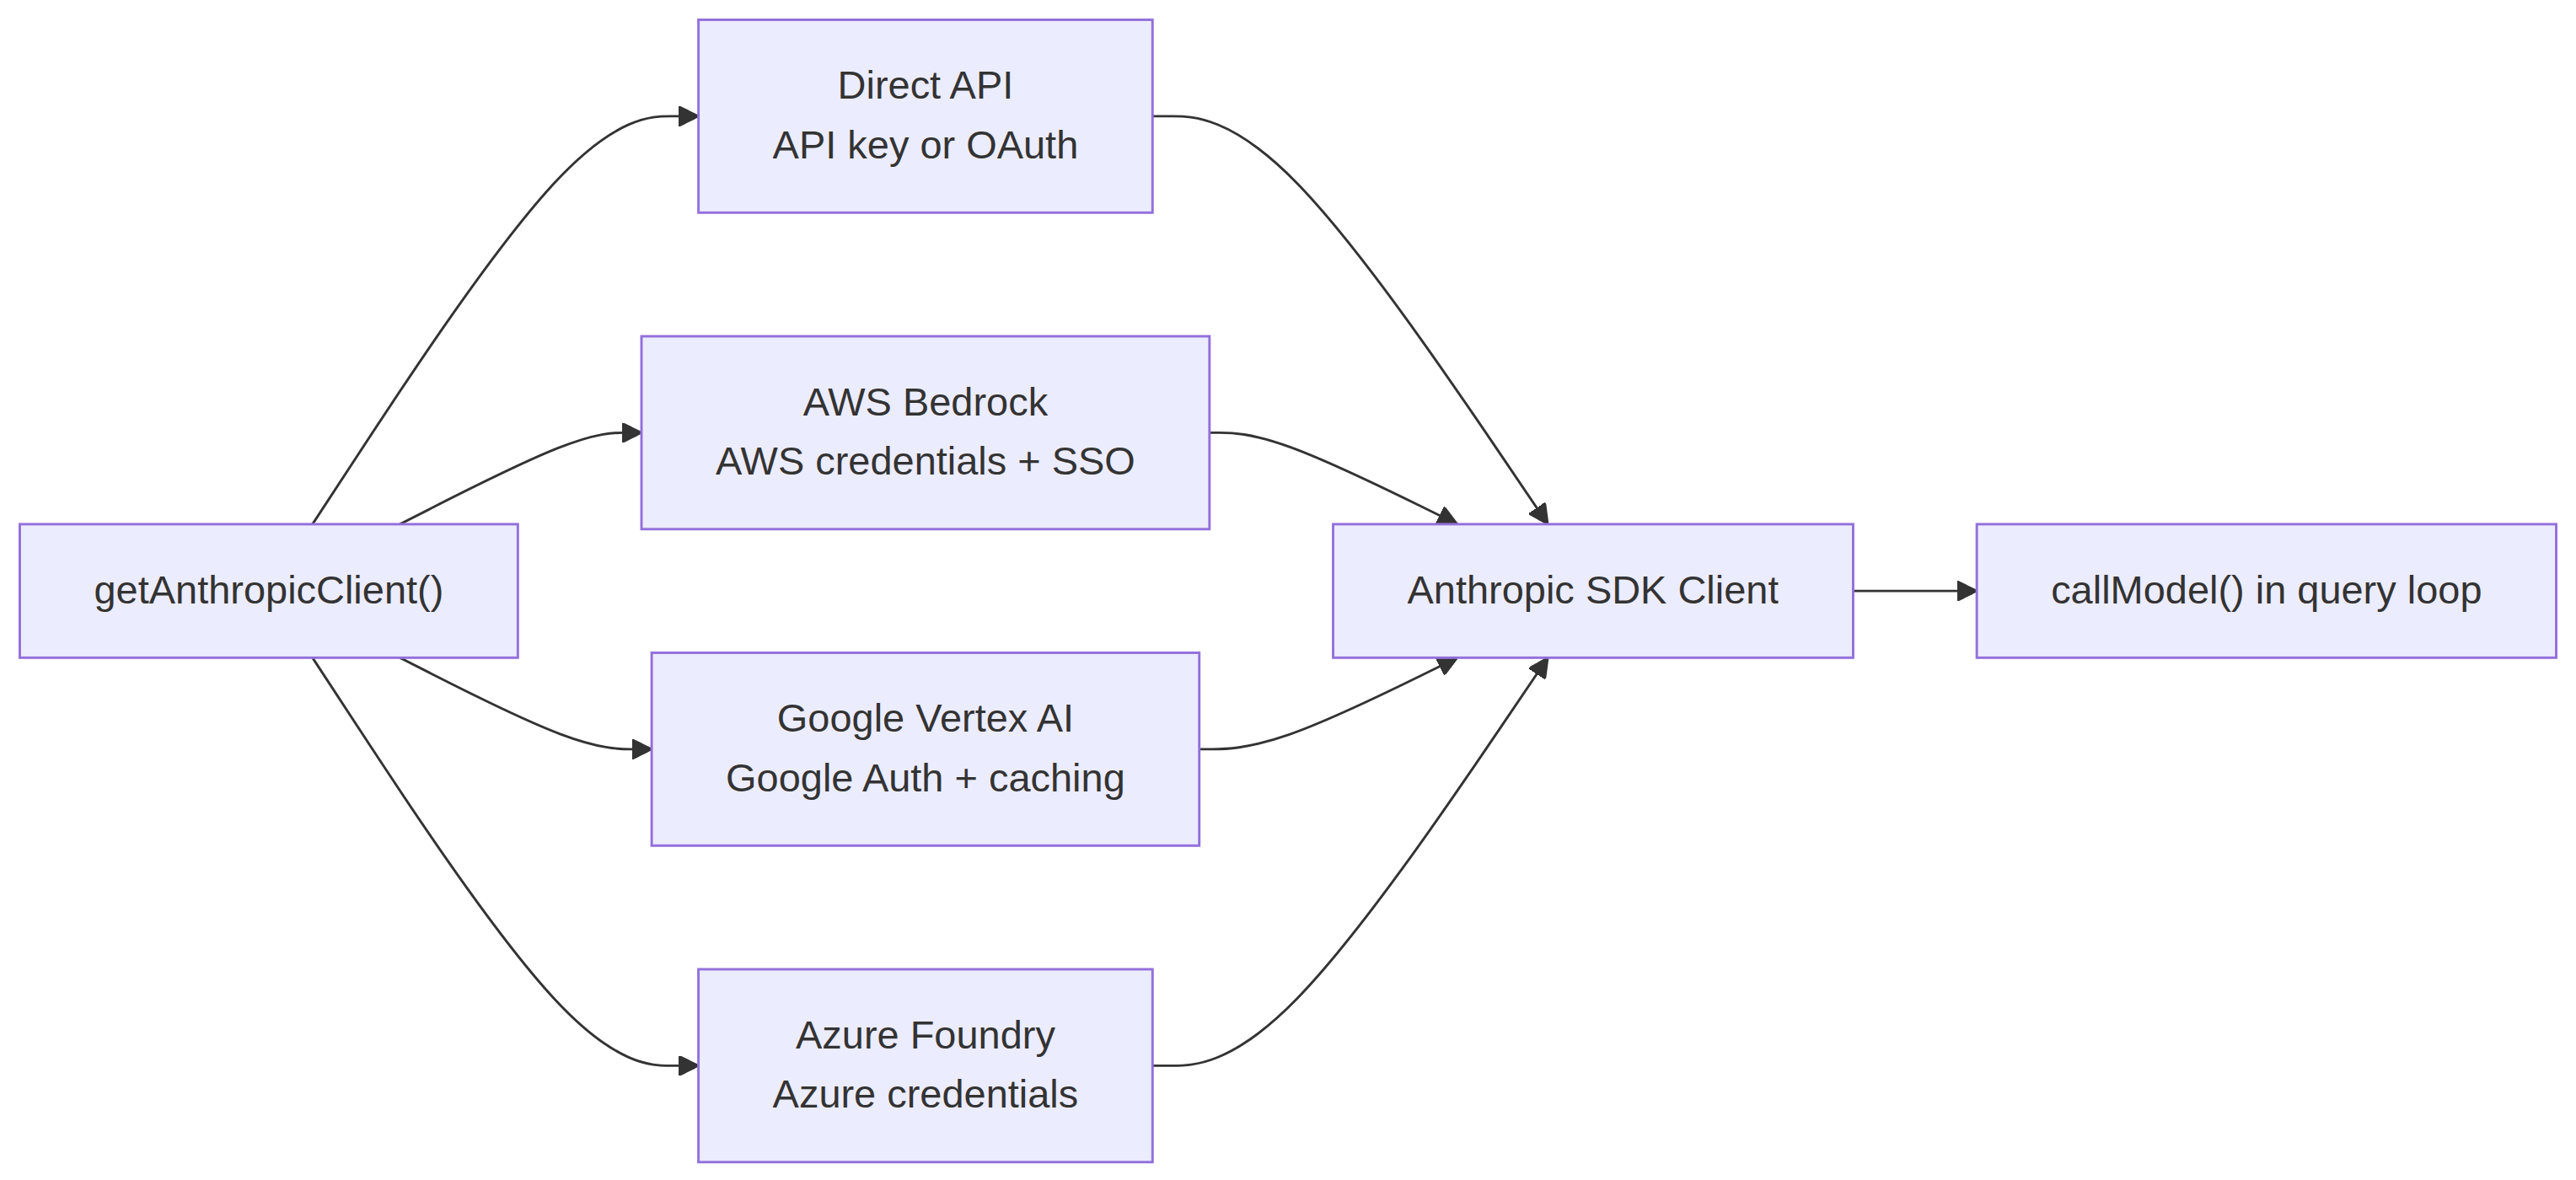
\includegraphics[width=10.85in,height=4.98in]{book/ch01-architecture_files/figure-latex/mermaid-figure-3.png}

The key insight is that the Anthropic SDK provides wrapper classes for
each cloud provider that present the same interface as the direct API
client. The \texttt{getAnthropicClient()} factory reads environment
variables and configuration to determine which provider to use,
constructs the appropriate client, and returns it. From that point
forward, \texttt{callModel()} and every other consumer treats it as a
generic Anthropic client.

Provider selection is determined at startup and stored in
\texttt{STATE}. The query loop never checks which provider is active.
This means switching from Direct API to Bedrock is a configuration
change, not a code change -- the agent loop, tool system, and permission
model are entirely provider-agnostic.

\begin{center}\rule{0.5\linewidth}{0.5pt}\end{center}

\section{The Build System}\label{the-build-system}

Claude Code ships as both an internal Anthropic tool and a public npm
package. The same codebase serves both, with compile-time feature flags
controlling what gets included.

\begin{Shaded}
\begin{Highlighting}[]
\CommentTok{// Conditional imports guarded by feature flags}
\KeywordTok{const}\NormalTok{ reactiveCompact }\OperatorTok{=} \FunctionTok{feature}\NormalTok{(}\StringTok{\textquotesingle{}REACTIVE\_COMPACT\textquotesingle{}}\NormalTok{)}
  \OperatorTok{?} \PreprocessorTok{require}\NormalTok{(}\StringTok{\textquotesingle{}./services/compact/reactiveCompact.js\textquotesingle{}}\NormalTok{)}
  \OperatorTok{:} \DataTypeTok{null}
\end{Highlighting}
\end{Shaded}

The \texttt{feature()} function comes from \texttt{bun:bundle}, Bun's
built-in bundler API. At build time, each feature flag resolves to a
boolean literal. The bundler's dead code elimination then strips the
\texttt{require()} call entirely when the flag is false -- the module is
never loaded, never included in the bundle, and never shipped.

The pattern is consistent: a top-level \texttt{feature()} guard wrapping
a \texttt{require()} call. The \texttt{require()} is used instead of
\texttt{import} specifically because dynamic \texttt{require()} can be
fully eliminated by the bundler when the guard is false, while dynamic
\texttt{import()} cannot (it returns a Promise that the bundler must
preserve).

There is an irony worth noting. The source maps published with early npm
releases contained \texttt{sourcesContent} -- the full original
TypeScript source, including the internal-only code paths. The feature
flags successfully stripped the runtime code but left the source in the
maps. This is how the Claude Code source became publicly readable.

\begin{center}\rule{0.5\linewidth}{0.5pt}\end{center}

\section{How the Pieces Connect}\label{how-the-pieces-connect}

The six abstractions form a dependency graph:

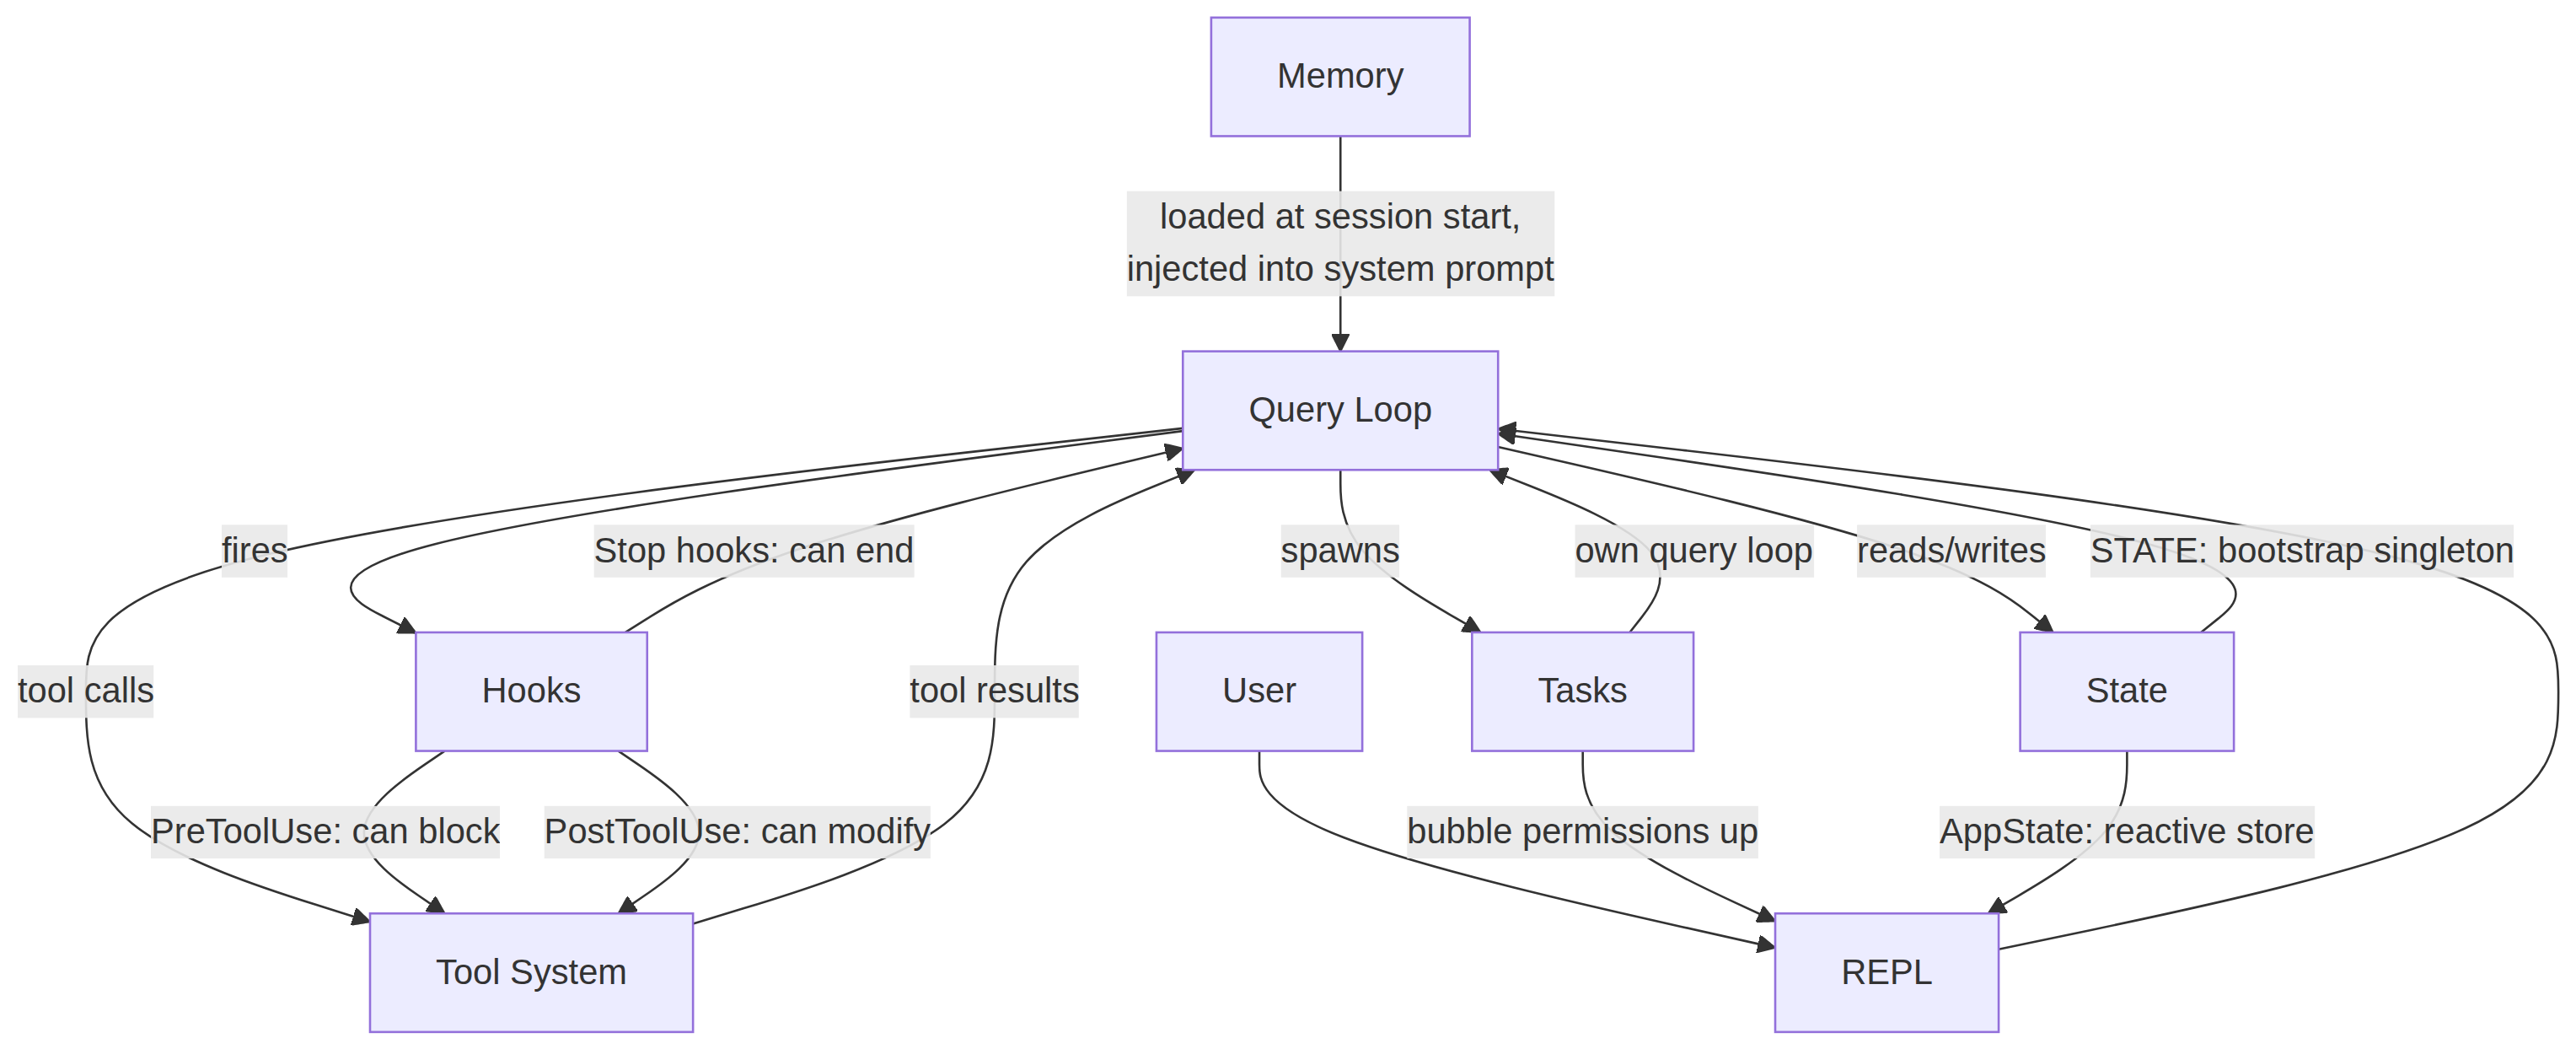
\includegraphics[width=12.22in,height=4.98in]{book/ch01-architecture_files/figure-latex/mermaid-figure-2.png}

Memory feeds into the query loop as part of the system prompt. The query
loop drives tool execution. Tool results feed back into the query loop
as messages. Tasks are recursive query loops with isolated message
histories. Hooks intercept the query loop at defined points. State is
read and written by everything, with the reactive store bridging to the
UI.

The circular dependency between the query loop and the tool system is
the system's defining characteristic. The model generates tool calls.
Tools execute and produce results. Results are appended to the message
history. The model sees the results and decides what to do next. This
cycle continues until the model stops generating tool calls or an
external constraint (token budget, max turns, user abort) terminates it.

Here is how they connect to the chapters that follow: the golden path
from input to output is the thread that runs through the entire book.
Chapter 2 traces how the system boots to the point where this path can
execute. Chapter 3 explains the two-tier state architecture that the
path reads and writes. Chapter 4 covers the API layer that the query
loop calls. Each subsequent chapter zooms into one segment of the path
you have just seen end-to-end.

\begin{center}\rule{0.5\linewidth}{0.5pt}\end{center}

\section{Apply This}\label{apply-this}

If you are building an agentic system -- any system where an LLM decides
what actions to take at runtime -- here are the patterns from Claude
Code's architecture that transfer.

\textbf{The generator loop pattern.} Use an async generator as your
agent loop, not callbacks or event emitters. The generator gives you
natural backpressure (consumers pull at their own pace), clean
cancellation (\texttt{.return()} on the generator), and a typed return
value for terminal states. The problem it solves: in callback-based
agent loops, it is difficult to know when the loop is ``done'' and why.
Generators make termination a first-class part of the type system.

\textbf{The self-describing tool interface.} Every tool should declare
its own concurrency safety, permission requirements, and rendering
behavior. Do not put this logic in a central orchestrator that ``knows
about'' each tool. The problem it solves: a central orchestrator becomes
a god object that must be updated every time a tool is added.
Self-describing tools scale linearly -- adding tool N+1 requires zero
changes to existing code.

\textbf{Separate infrastructure state from reactive state.} Not all
state needs to trigger UI updates. Session configuration, cost tracking,
and telemetry belong in a plain mutable object. Message history,
progress indicators, and approval queues belong in a reactive store. The
problem it solves: making everything reactive adds subscription overhead
and complexity to state that changes once at startup and is read a
thousand times. Two tiers match two access patterns.

\textbf{Permission modes, not permission checks.} Define a small set of
named modes (plan, default, auto, bypass) and resolve every permission
decision through the mode. Do not scatter \texttt{if\ (isAllowed)}
checks through tool implementations. The problem it solves: inconsistent
permission enforcement. When every tool goes through the same mode-based
resolution chain, you can reason about the system's security posture by
knowing which mode is active.

\textbf{Recursive agent architecture via tasks.} Sub-agents should be
new instances of the same agent loop with their own message history, not
special-cased code paths. Permission escalation flows upward via
\texttt{bubble} mode. The problem it solves: sub-agent logic that
diverges from the main agent loop, leading to subtle differences in
behavior and error handling. If the sub-agent is the same loop, it
inherits all the same guarantees.

\chapter{Chapter 2: Starting Fast -- The Bootstrap
Pipeline}\label{chapter-2-starting-fast-the-bootstrap-pipeline}

If Chapter 1 gave you the map of Claude Code's architecture, this
chapter gives you the route it takes to reach a working state. Every
component from the six abstractions -- the query loop, the tool system,
the state layers, hooks, memory -- must be initialized before the user
sees a cursor. The budget for all of it: 300 milliseconds.

Three hundred milliseconds is the threshold where humans perceive a tool
as instant. Cross it, and the CLI feels sluggish. Miss it by a lot, and
developers stop using it. Everything in this chapter exists to stay
under that line.

Bootstrap must accomplish four things: validate the environment,
establish security boundaries, configure the communication layer, and
render the UI. It must do all four in under 300ms. The architectural
insight is that these four jobs can be partially overlapped, carefully
ordered, and aggressively pruned to fit inside a budget that feels
impossible for a system this complex.

A note on methodology: the timestamps in this chapter are approximate,
derived from the codebase's own profiling checkpoints. They represent
typical warm-start timings on modern hardware. Cold starts are slower.
The absolute numbers matter less than the relative structure: which
operations overlap, which block, and which are deferred.

\begin{center}\rule{0.5\linewidth}{0.5pt}\end{center}

\section{The Shape of the Pipeline}\label{the-shape-of-the-pipeline}

The startup pipeline lives in five files, executed in sequence. Each
file narrows the scope of what the system needs to do next:

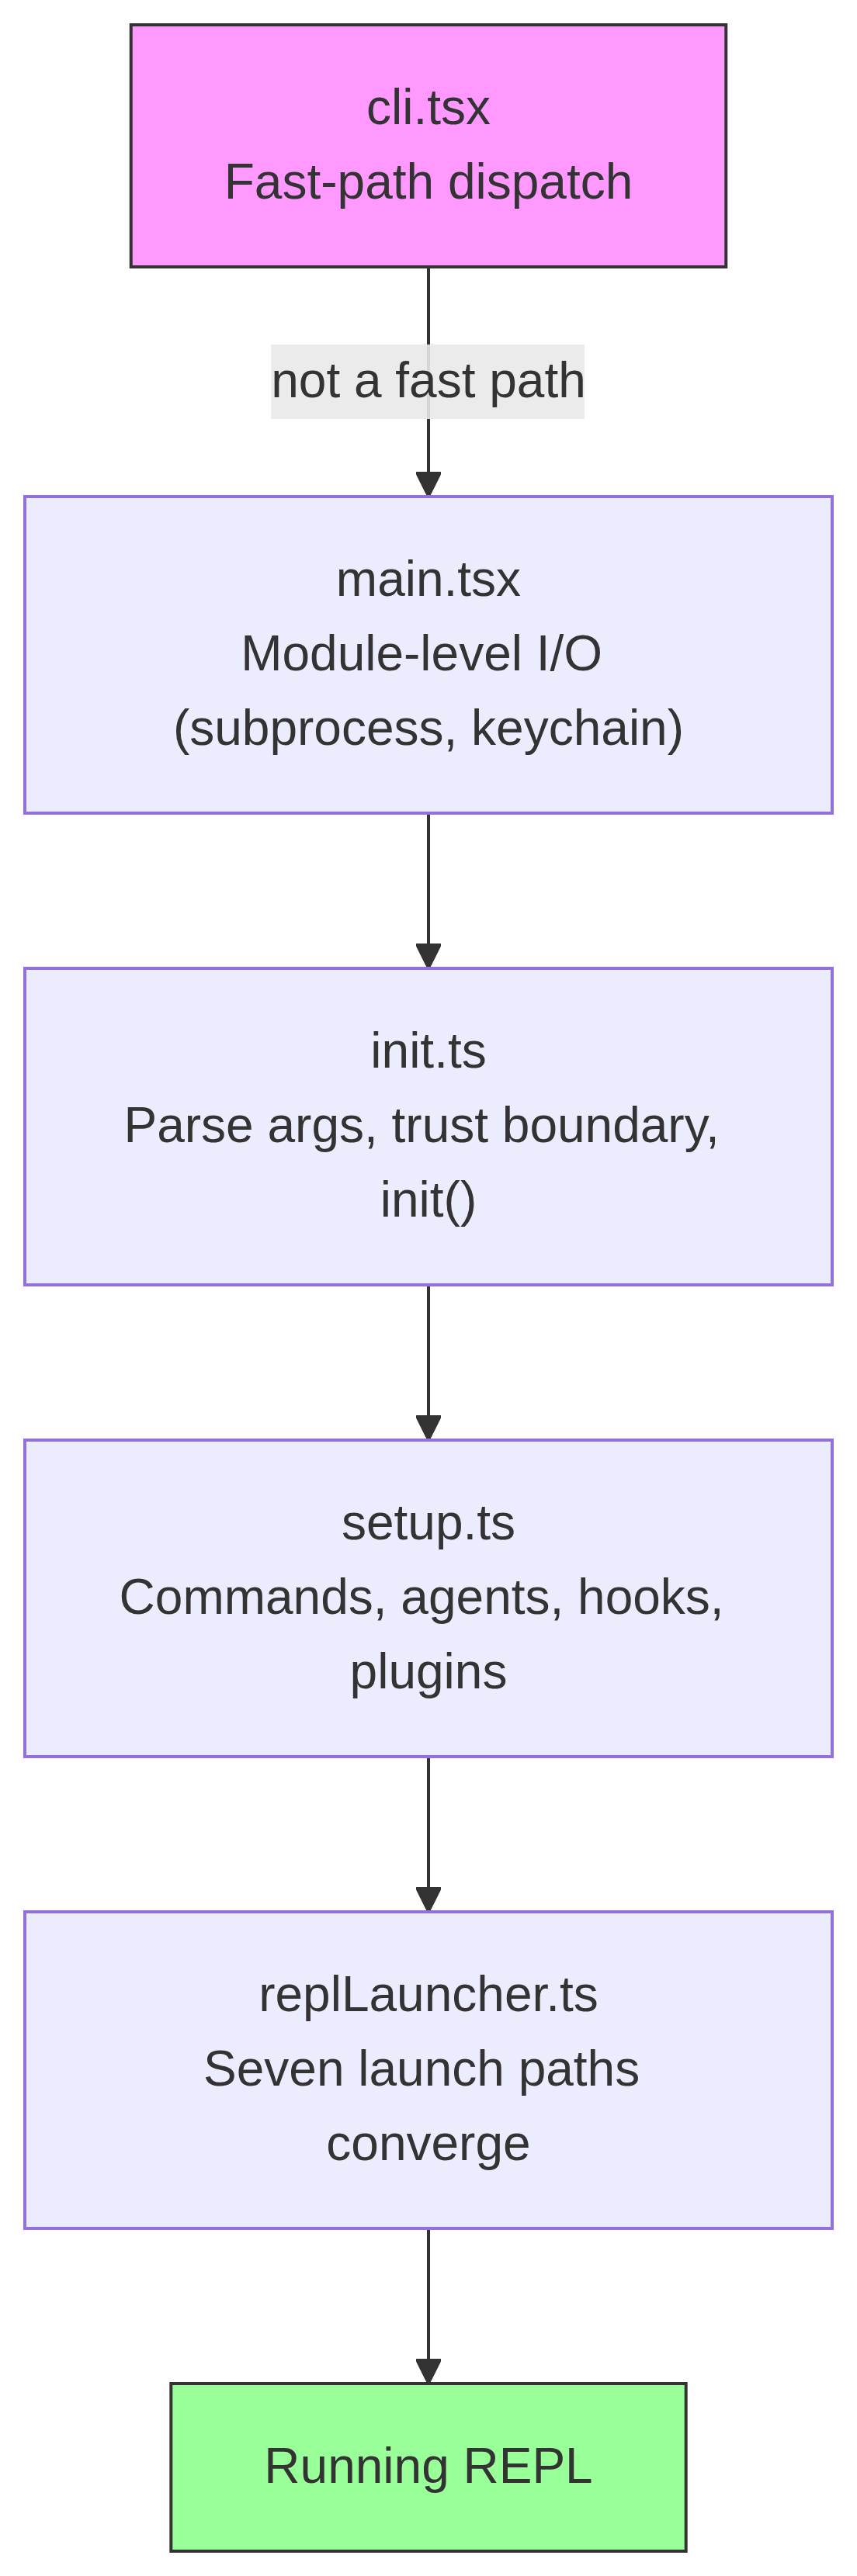
\includegraphics[width=2.88in,height=8.65in]{book/ch02-bootstrap_files/figure-latex/mermaid-figure-1.png}

Each file does the minimum work necessary before passing control to the
next. \texttt{cli.tsx} tries to exit before importing anything heavy.
\texttt{main.tsx} fires slow operations as side effects during import
evaluation. \texttt{init.ts} resolves configuration and establishes the
trust boundary. \texttt{setup.ts} registers capabilities.
\texttt{replLauncher.ts} picks the right entry point and starts the UI.

Three parallelism strategies make this fast:

\begin{enumerate}
\def\labelenumi{\arabic{enumi}.}
\tightlist
\item
  \textbf{Module-level subprocess dispatch.} Fire keychain and MDM reads
  as side effects \emph{during import evaluation}. The subprocesses run
  while the remaining \textasciitilde135ms of static imports load.
\item
  \textbf{Promise parallelism in setup.} Socket binding, hook
  snapshotting, command loading, and agent definition loading all run
  concurrently.
\item
  \textbf{Post-render deferred prefetches.} Everything the user does not
  need before typing their first message -- git status, model
  capabilities, AWS credentials -- runs after the prompt is visible.
\end{enumerate}

A fourth strategy is less visible but equally important: \textbf{dynamic
imports to defer module evaluation}. The codebase uses
\texttt{await\ import(\textquotesingle{}./module.js\textquotesingle{})}
in at least a dozen places to avoid loading code until it is needed.
OpenTelemetry (400KB + 700KB gRPC) loads only when telemetry
initializes. React components load only when rendering. Each dynamic
import trades cold-path latency (first use triggers module evaluation)
for hot-path speed (startup does not pay for modules it might never
use).

\begin{center}\rule{0.5\linewidth}{0.5pt}\end{center}

\section{Phase 0: Fast-Path Dispatch
(cli.tsx)}\label{phase-0-fast-path-dispatch-cli.tsx}

The first file the process enters, \texttt{cli.tsx}, has one job:
determine whether the full bootstrap pipeline is needed at all. Many
invocations -- \texttt{claude\ -\/-version}, \texttt{claude\ -\/-help},
\texttt{claude\ mcp\ list} -- need a specific answer and nothing else.
Loading React, initializing telemetry, reading the keychain, and setting
up the tool system would be pure waste.

The pattern is: check \texttt{argv}, dynamically import only the handler
you need, and exit before the rest of the system loads.

\begin{Shaded}
\begin{Highlighting}[]
\CommentTok{// Pseudocode for the fast{-}path pattern}
\ControlFlowTok{if}\NormalTok{ (args}\OperatorTok{.}\AttributeTok{length} \OperatorTok{===} \DecValTok{1} \OperatorTok{\&\&}\NormalTok{ args[}\DecValTok{0}\NormalTok{] }\OperatorTok{===} \StringTok{\textquotesingle{}{-}{-}version\textquotesingle{}}\NormalTok{) \{}
  \KeywordTok{const}\NormalTok{ \{ printVersion \} }\OperatorTok{=} \ControlFlowTok{await} \ImportTok{import}\NormalTok{(}\StringTok{\textquotesingle{}./commands/version.js\textquotesingle{}}\NormalTok{)}
  \ControlFlowTok{await} \FunctionTok{printVersion}\NormalTok{()}
  \BuiltInTok{process}\OperatorTok{.}\FunctionTok{exit}\NormalTok{(}\DecValTok{0}\NormalTok{)}
\NormalTok{\}}
\end{Highlighting}
\end{Shaded}

There are roughly a dozen fast paths covering version, help,
configuration, MCP server management, and update checks. The specifics
do not matter -- the pattern does. Each path dynamically imports exactly
one module, calls one function, and exits. The rest of the codebase
never loads.

This is the first instance of a principle that recurs throughout
bootstrap: \textbf{do less by knowing more about intent}. The argv array
reveals the user's intent. If the intent is narrow, the execution path
should be narrow too.

If no fast path matches, \texttt{cli.tsx} falls through to the full
\texttt{main.tsx} import, and the real startup begins.

\begin{center}\rule{0.5\linewidth}{0.5pt}\end{center}

\section{Phase 1: Module-Level I/O
(main.tsx)}\label{phase-1-module-level-io-main.tsx}

When \texttt{main.tsx} is imported, its module-level side effects fire
during evaluation -- before any function in the file is called. This is
the most performance-critical technique in the entire bootstrap:

\begin{Shaded}
\begin{Highlighting}[]
\CommentTok{// These run at import time, not at call time}
\KeywordTok{const}\NormalTok{ mdmPromise }\OperatorTok{=} \FunctionTok{startMDMSubprocess}\NormalTok{()}
\KeywordTok{const}\NormalTok{ keychainPromise }\OperatorTok{=} \FunctionTok{readKeychainCredentials}\NormalTok{()}
\end{Highlighting}
\end{Shaded}

While the JavaScript engine evaluates the rest of \texttt{main.tsx} and
its transitive imports (\textasciitilde138ms of module evaluation),
these two promises are already in flight. The MDM (Mobile Device
Management) subprocess checks organizational security policies. The
keychain read fetches stored credentials. Both are I/O-bound operations
that would otherwise serialize on the critical path.

The insight: module evaluation is not idle time -- it is time you can
overlap with I/O. By the time \texttt{main.tsx}'s exported functions are
first called, these promises are often already resolved.

This technique requires suppressing ESLint's top-level-await and
side-effect-in-module-scope rules in the relevant files. The codebase
has a custom ESLint rule specifically for \texttt{process.env} access
patterns that allows controlled side effects at module scope while
preventing uncontrolled ones elsewhere.

\begin{center}\rule{0.5\linewidth}{0.5pt}\end{center}

\section{Phase 2: Parse and Trust
(init.ts)}\label{phase-2-parse-and-trust-init.ts}

The \texttt{init()} function is memoized -- calling it multiple times is
safe and returns the same result. This is important because multiple
entry points (the REPL, print mode, SDK mode) may each call
\texttt{init()}, and the memoization guarantees it runs exactly once.

The function resolves command-line arguments via Commander, loads
configuration from multiple sources (global settings, project settings,
environment variables), and then hits the most important boundary in the
pipeline.

\subsection{The Trust Boundary}\label{the-trust-boundary}

Before the trust boundary, the system operates in a restricted mode.
After it, full capabilities are available. The boundary exists because
Claude Code reads environment variables -- and environment variables can
be poisoned.

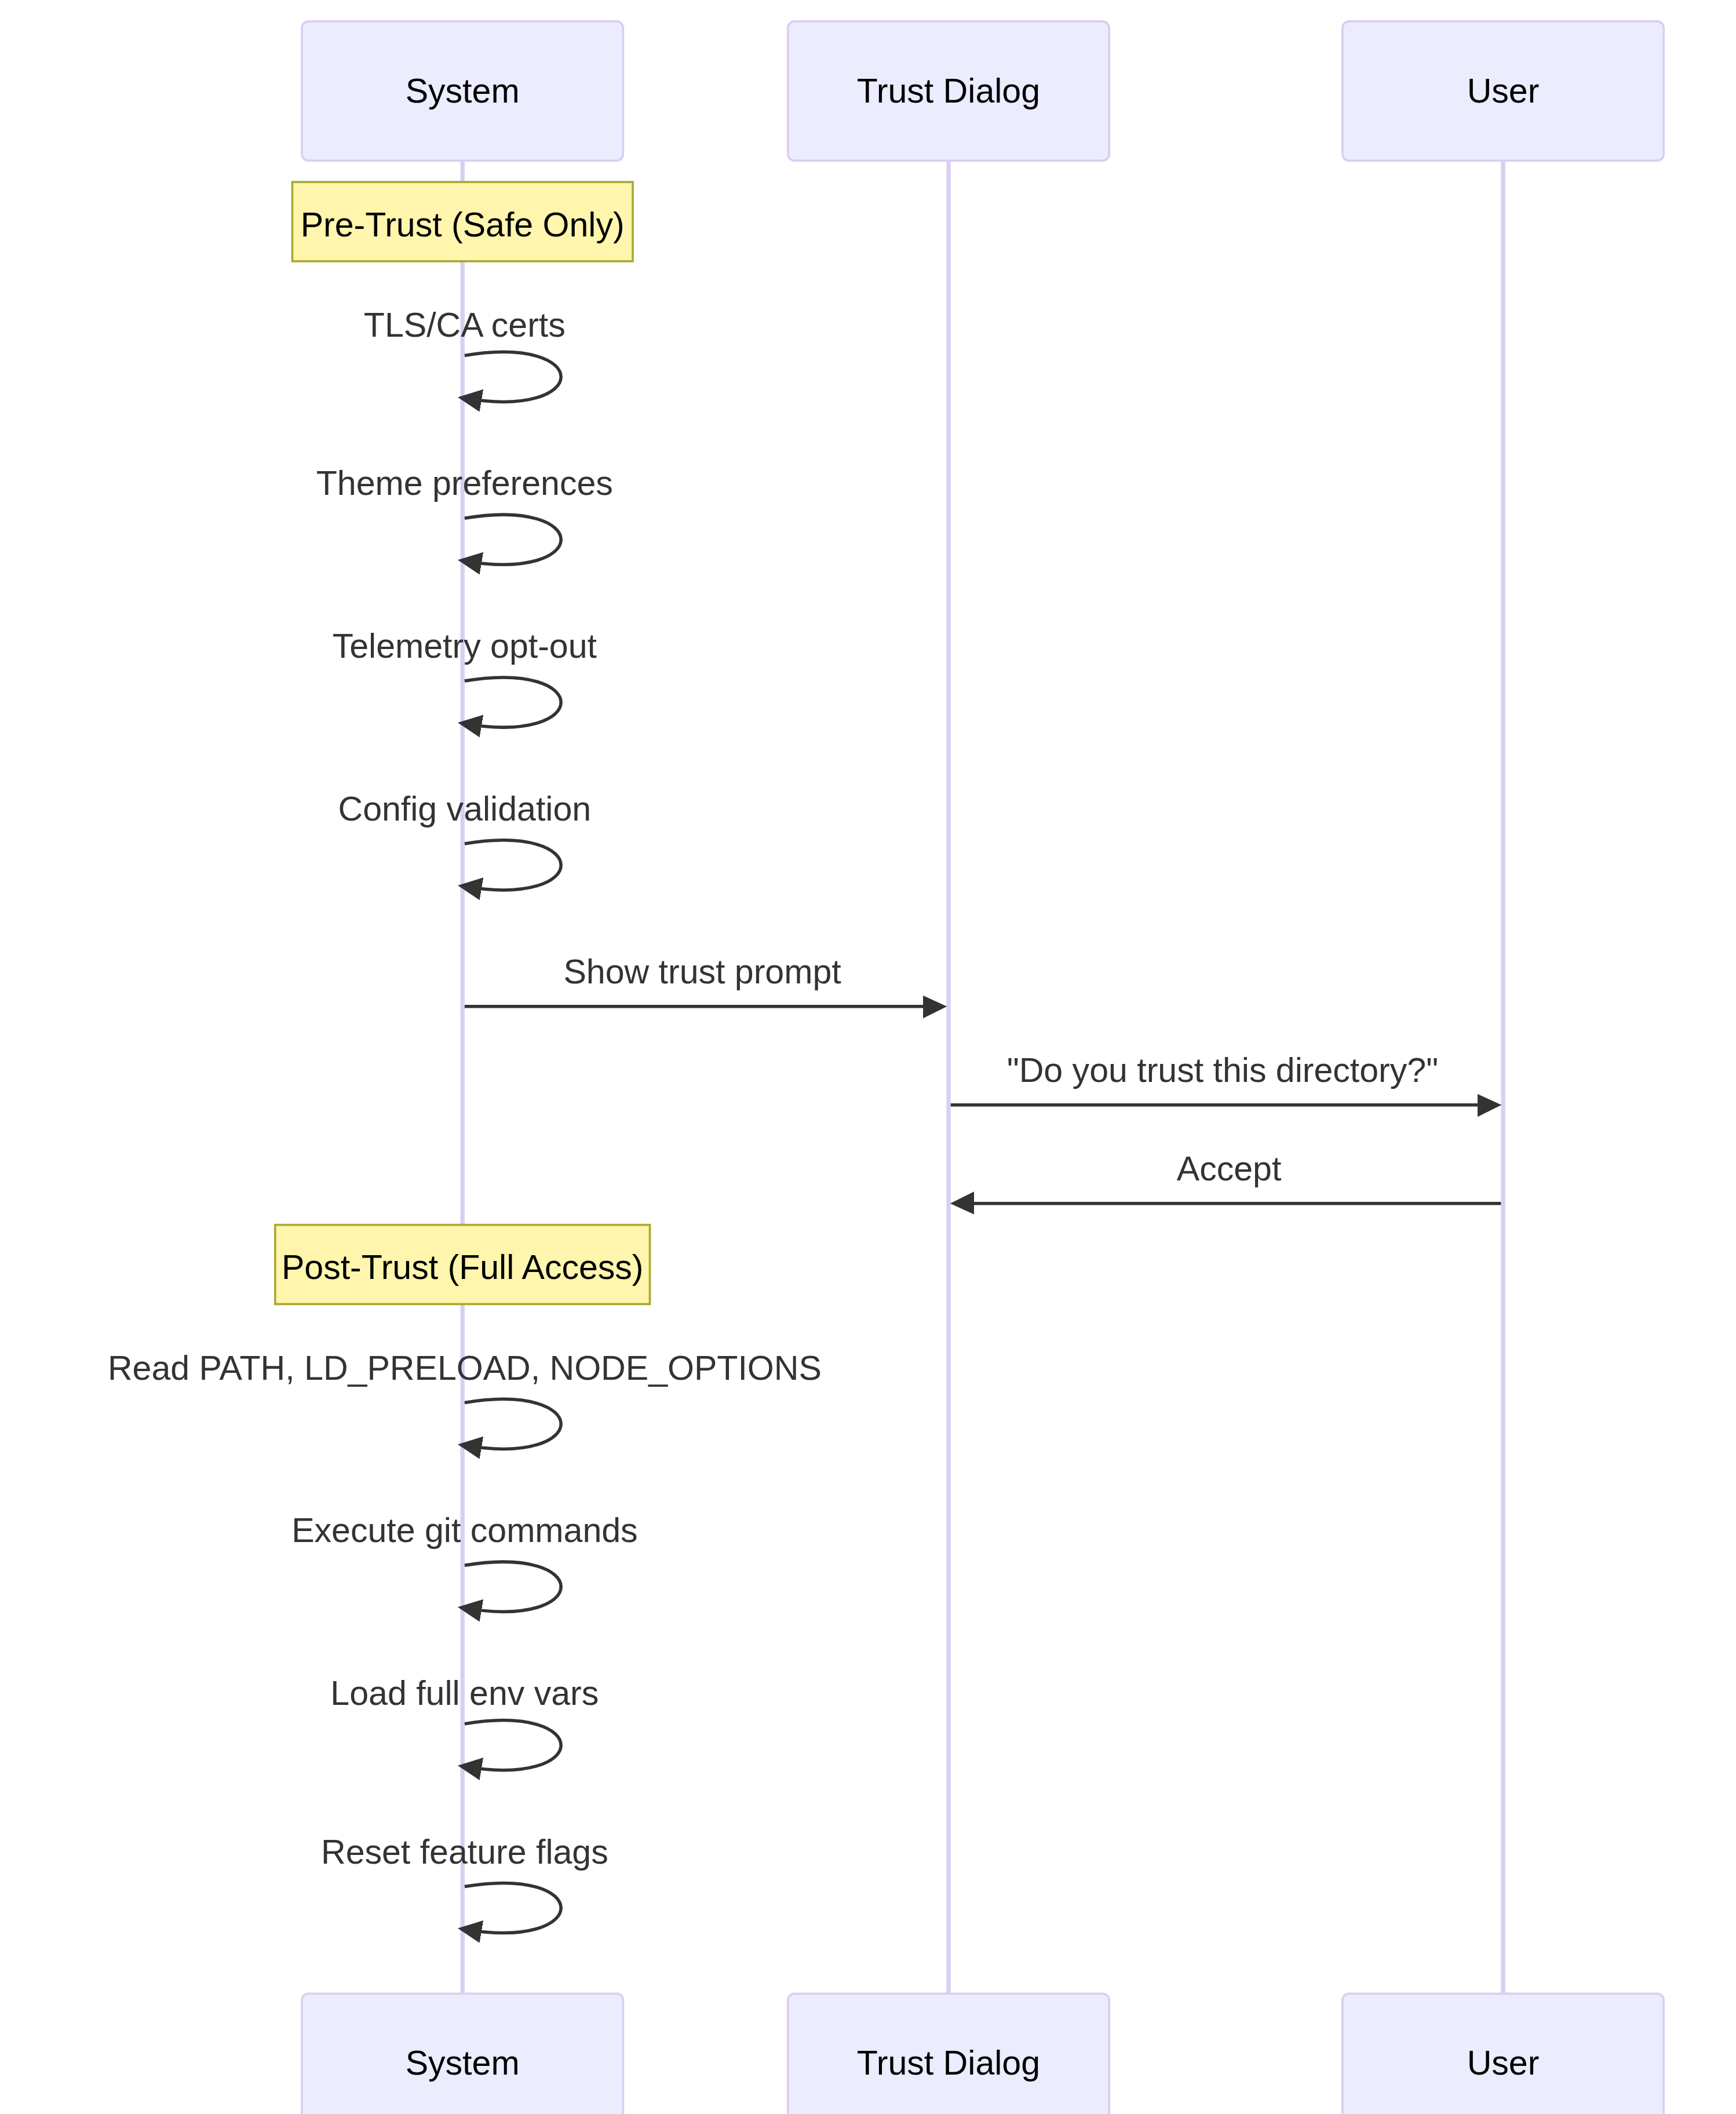
\includegraphics[width=8.61in,height=10.49in]{book/ch02-bootstrap_files/figure-latex/mermaid-figure-4.png}

The trust boundary is not about the user trusting Claude Code. It is
about Claude Code trusting the \emph{environment}. A malicious
\texttt{.bashrc} could set \texttt{LD\_PRELOAD} to inject code into
every subprocess. The trust dialog ensures the user explicitly consents
to operating in a directory that may have been configured by someone
else.

The system has ten distinct trust-sensitive operations. Before the user
accepts the trust dialog, only safe operations run: TLS certificate
configuration, theme preferences, telemetry opt-out. After trust, the
system reads potentially dangerous environment variables (PATH,
LD\_PRELOAD, NODE\_OPTIONS), executes git commands, and applies the full
environment configuration.

\subsection{The preAction Hook}\label{the-preaction-hook}

Commander's \texttt{preAction} hook is the architectural linchpin.
Commander parses the command structure (flags, subcommands, positional
arguments) \emph{without} executing anything. The \texttt{preAction}
hook fires after parsing but before the matched command handler runs:

\begin{Shaded}
\begin{Highlighting}[]
\NormalTok{program}\OperatorTok{.}\FunctionTok{hook}\NormalTok{(}\StringTok{\textquotesingle{}preAction\textquotesingle{}}\OperatorTok{,} \KeywordTok{async}\NormalTok{ (thisCommand) }\KeywordTok{=\textgreater{}}\NormalTok{ \{}
  \ControlFlowTok{await} \FunctionTok{init}\NormalTok{(thisCommand)}
\NormalTok{\})}
\end{Highlighting}
\end{Shaded}

This separation means fast-path commands (handled in \texttt{cli.tsx}
before Commander loads) never pay the \texttt{init()} cost. Only
commands that need the full environment trigger initialization.

\begin{center}\rule{0.5\linewidth}{0.5pt}\end{center}

\section{Phase 3: Setup (setup.ts)}\label{phase-3-setup-setup.ts}

After \texttt{init()} completes, \texttt{setup()} registers all the
capabilities the system needs:

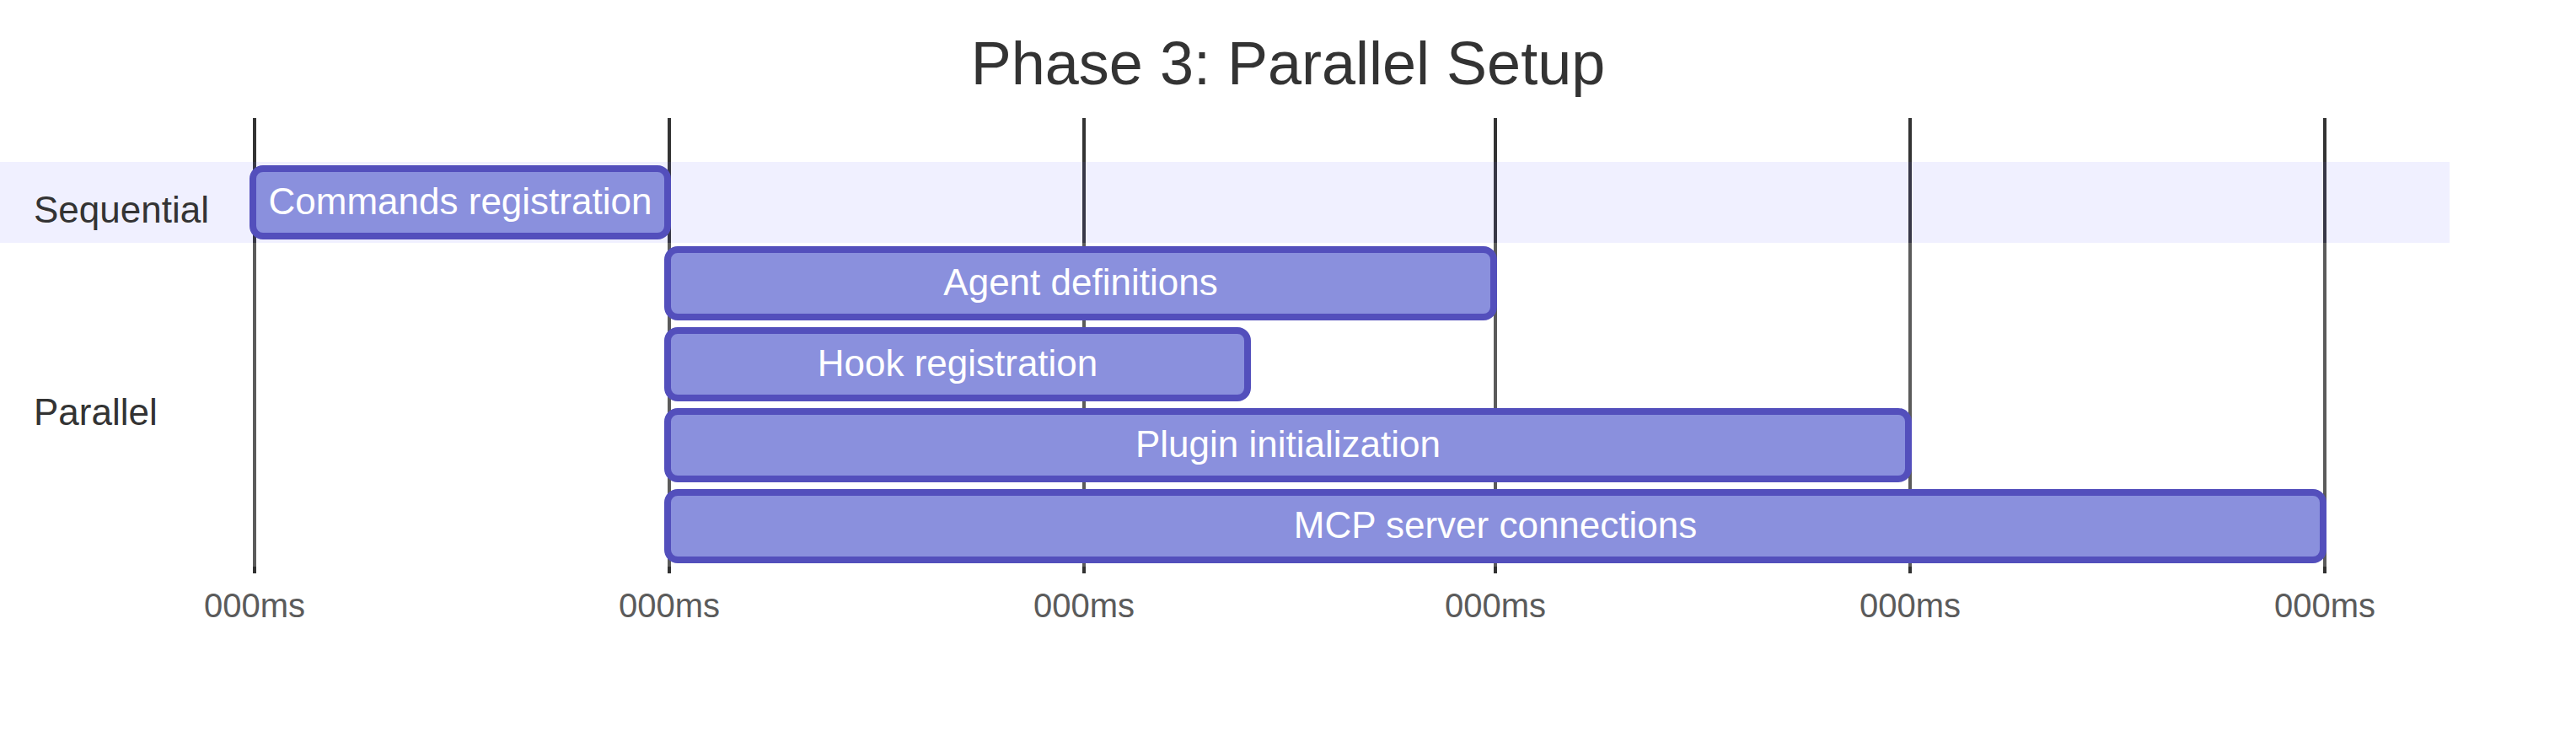
\includegraphics[width=7.96in,height=2.29in]{book/ch02-bootstrap_files/figure-latex/mermaid-figure-3.png}

Commands, agents, hooks, and plugins all register in parallel where
possible. The setup phase is where the system transitions from ``I know
my configuration'' to ``I have all my capabilities.'' After setup, every
tool is registered, every hook is wired, and the system is ready to
handle user input.

Setup also handles the security hook snapshot. The hook configuration is
read from disk once, frozen into an immutable snapshot, and used for the
rest of the session. Later modifications to the hooks configuration file
on disk are ignored. This prevents an attacker from modifying hook rules
after the session starts -- the frozen snapshot is the only source of
truth for permission decisions.

\begin{center}\rule{0.5\linewidth}{0.5pt}\end{center}

\section{Phase 4: Launch
(replLauncher.ts)}\label{phase-4-launch-repllauncher.ts}

Seven different code paths converge on \texttt{replLauncher.ts}:
interactive REPL, print mode (\texttt{-\/-print}), SDK mode, resume
(\texttt{-\/-resume}), continue (\texttt{-\/-continue}), pipe mode, and
headless. The launcher inspects the configuration produced by
\texttt{init()} and dispatches to the right entry point.

Two examples illustrate the range:

\textbf{Interactive REPL} -- the standard case. The launcher mounts the
React/Ink component tree, starts the terminal renderer, and enters the
event loop. The user sees a prompt and can start typing.

\textbf{Print mode} (\texttt{-\/-print}) -- a single prompt from argv.
The launcher creates a headless query loop with no React tree, runs it
to completion, streams the output to stdout, and exits. Same agent loop,
different presentation.

The important detail: all seven paths eventually call \texttt{query()}
-- the same agent loop from Chapter 1. The launch path determines
\emph{how} the loop is presented (interactive terminal, single-shot, SDK
protocol), not \emph{what} it does. This convergence is what makes the
architecture testable and predictable: regardless of how the user
invokes Claude Code, the core behavior is identical.

\begin{center}\rule{0.5\linewidth}{0.5pt}\end{center}

\section{The Startup Timeline}\label{the-startup-timeline}

Here is what the full pipeline looks like in time:

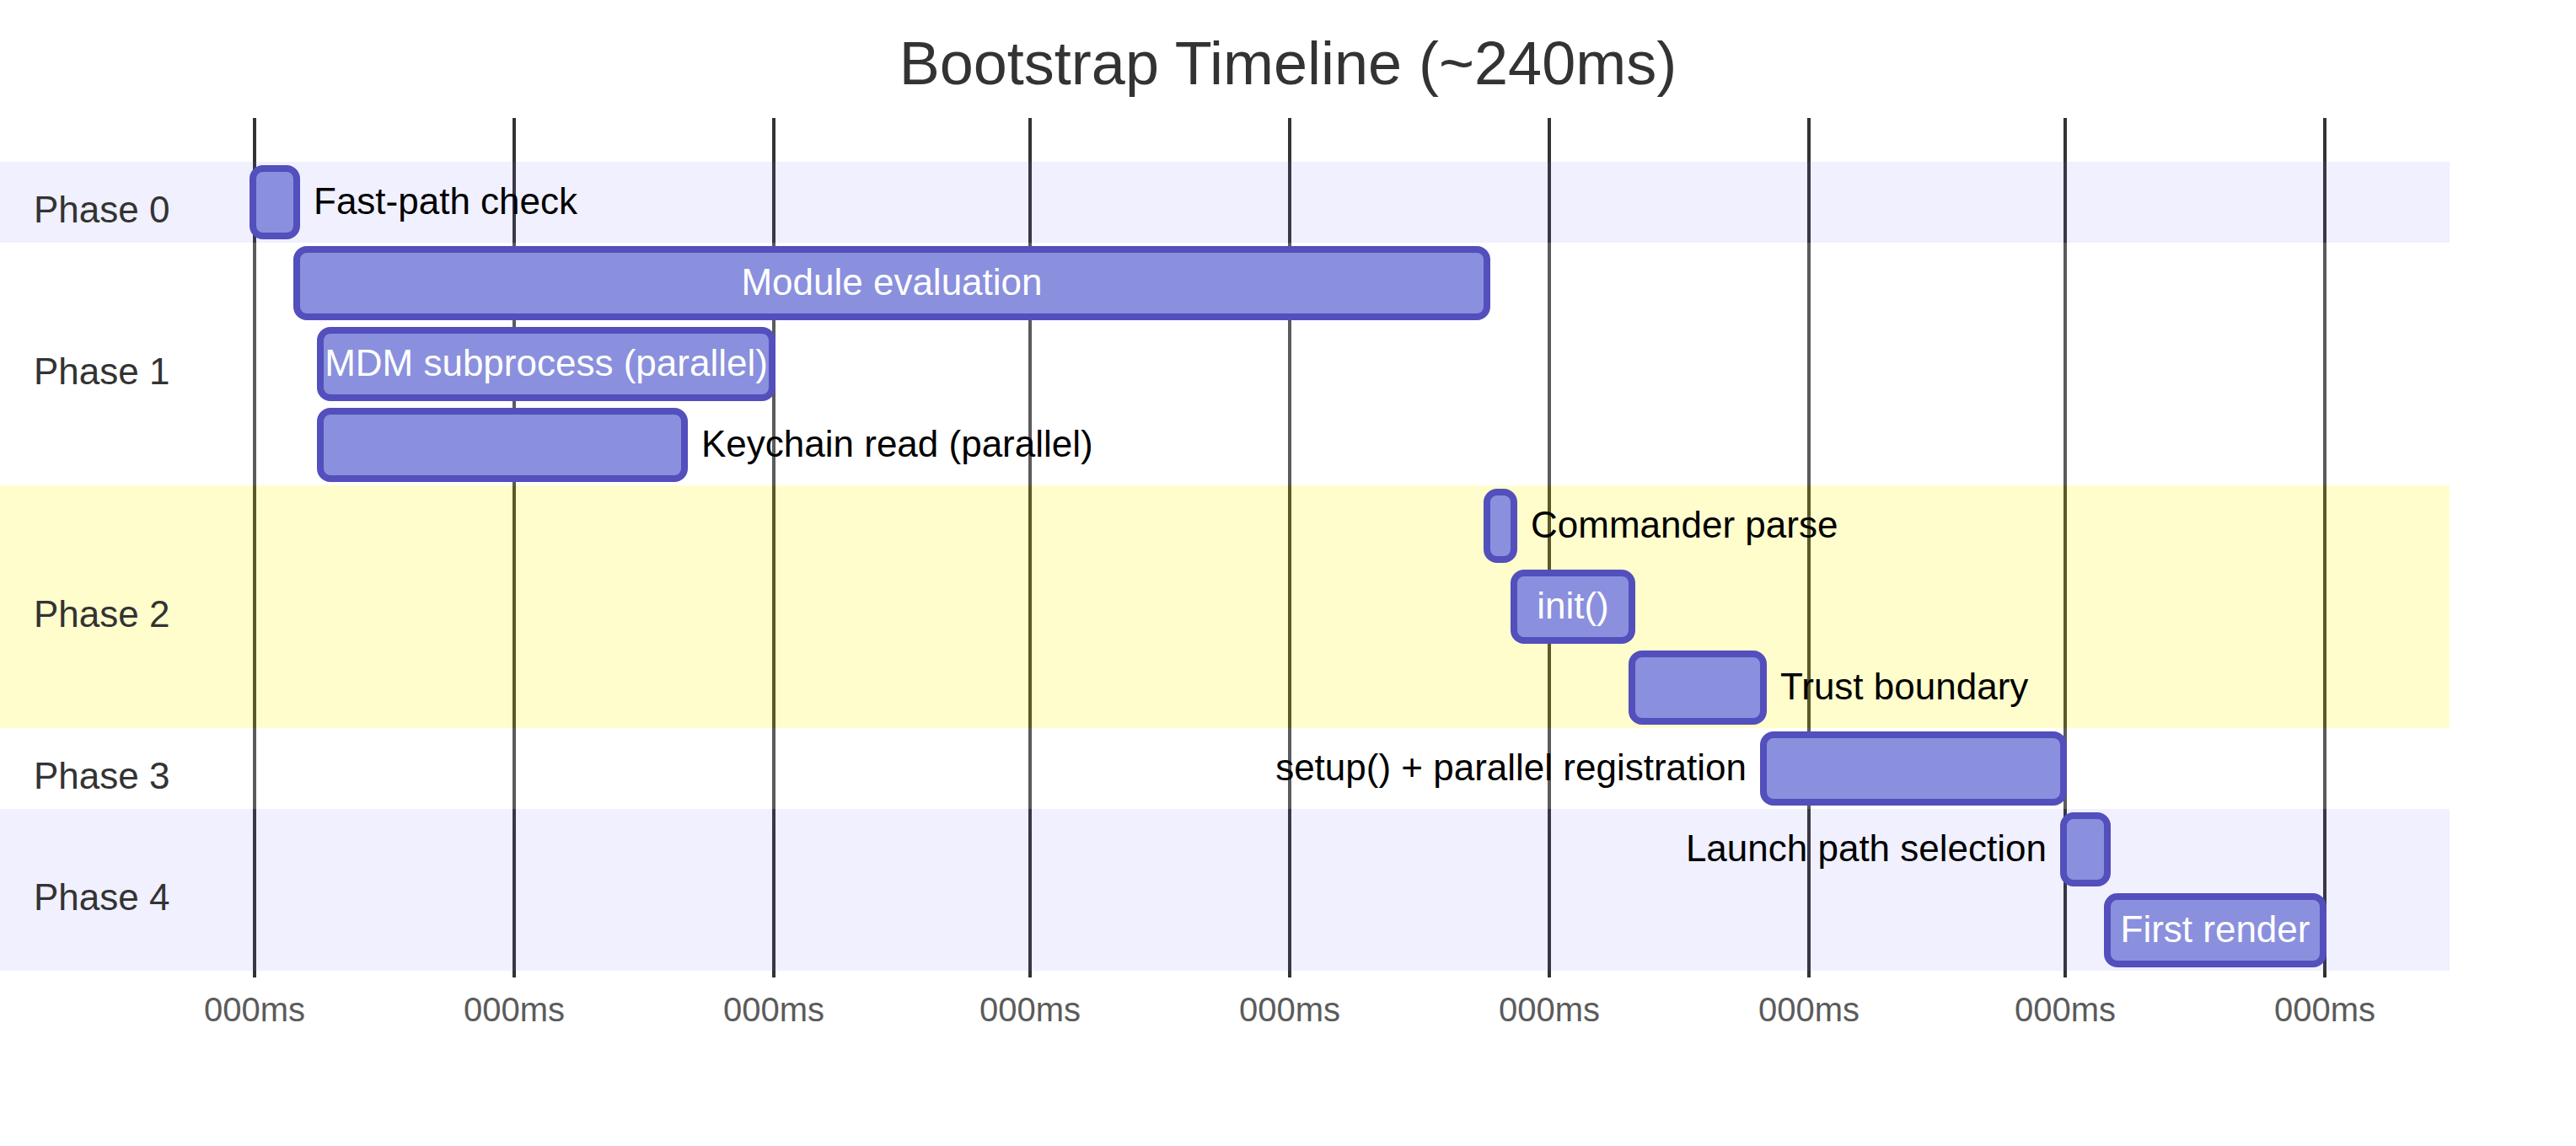
\includegraphics[width=7.96in,height=3.54in]{book/ch02-bootstrap_files/figure-latex/mermaid-figure-2.png}

The critical path runs through module evaluation (the single longest
phase at \textasciitilde138ms), then Commander parse, init, and setup.
The parallel I/O operations (MDM, keychain) overlap with module
evaluation and are typically resolved before they are needed.

\subsection{The Performance Budget}\label{the-performance-budget}

\begin{longtable}[]{@{}lll@{}}
\toprule\noalign{}
Phase & Time & What Happens \\
\midrule\noalign{}
\endhead
\bottomrule\noalign{}
\endlastfoot
Fast-path check & \textasciitilde5ms & Check argv, exit early if
possible \\
Module evaluation & \textasciitilde138ms & Import tree, fire parallel
I/O \\
Commander parse & \textasciitilde3ms & Parse flags and subcommands \\
init() & \textasciitilde14ms & Config resolution, trust boundary \\
setup() & \textasciitilde35ms & Commands, agents, hooks, plugins \\
Launch + first render & \textasciitilde25ms & Pick path, mount React,
first paint \\
\textbf{Total} & \textbf{\textasciitilde240ms} & Under 300ms budget \\
\end{longtable}

The total is approximately 240ms on a modern machine -- 60ms of headroom
under the 300ms budget. Cold starts (first run after reboot, OS cache
empty) can push module evaluation to 200ms+, bringing the total closer
to the limit.

\begin{center}\rule{0.5\linewidth}{0.5pt}\end{center}

\section{The Migration System}\label{the-migration-system}

A brief note on one subsystem that runs during init: schema migrations.
Claude Code stores configuration and session data in local files and
directories. When the format changes between versions, migrations run
automatically at startup.

Each migration is a function with a version number. The system checks
the current schema version against the highest migration version, runs
pending migrations in order, and updates the version. Migrations are
idempotent and fast (operating on small local files, not databases). The
entire migration pass typically completes in under 5ms. If a migration
fails, it logs the error and continues -- availability beats strict
consistency for local configuration.

\begin{center}\rule{0.5\linewidth}{0.5pt}\end{center}

\section{What Startup Teaches About System
Design}\label{what-startup-teaches-about-system-design}

The bootstrap pipeline is a study in narrowing scopes. Each phase
reduces the space of possibilities:

\begin{itemize}
\tightlist
\item
  Phase 0 narrows from ``any CLI invocation'' to ``needs full
  bootstrap''
\item
  Phase 1 narrows from ``everything must load'' to ``load in parallel
  with I/O''
\item
  Phase 2 narrows from ``unknown environment'' to ``trusted, configured
  environment''
\item
  Phase 3 narrows from ``no capabilities'' to ``fully registered''
\item
  Phase 4 narrows from ``seven possible modes'' to ``one concrete launch
  path''
\end{itemize}

By the time the REPL renders, every decision has been made. The query
loop receives a fully configured environment with no ambiguity about
what mode it is in, which tools are available, or what permissions
apply. The 300ms budget is not just a performance target -- it is a
forcing function that prevents bootstrap from becoming a lazy
initialization system where decisions are deferred and scattered
throughout the codebase.

\begin{center}\rule{0.5\linewidth}{0.5pt}\end{center}

\section{Apply This}\label{apply-this-1}

\textbf{Overlap I/O with initialization.} Fire slow operations
(subprocess spawns, credential reads, network checks) at module
evaluation time, before they are needed. The JavaScript engine is doing
synchronous work anyway -- use that time for parallel I/O. The pattern:
\texttt{const\ promise\ =\ startSlowThing()} at the top of the file,
\texttt{await\ promise} at the point of use.

\textbf{Narrow scope as early as possible.} The bootstrap pipeline's
five files form a funnel: each phase eliminates work that subsequent
phases do not need to do. Fast-path dispatch is the most dramatic
example, but the principle applies everywhere. If you can determine at
parse time that a code path is unnecessary, skip it.

\textbf{Establish trust boundaries explicitly.} If your application
reads from an environment it does not control (environment variables,
configuration files, shell settings), draw a clear line between ``safe
to read before the user consents'' and ``only read after consent.'' The
trust boundary prevents a class of attacks where a malicious environment
poisons the application before the user has a chance to evaluate it.

\textbf{Memoize your init function.} Make initialization idempotent --
calling it twice produces the same result. This eliminates ordering bugs
when multiple entry points may each trigger initialization. The
memoization pattern is trivial but eliminates an entire class of
double-initialization bugs.

\textbf{Capture early input before yielding.} In an event-driven system,
user input that arrives during initialization can be lost. Claude Code
captures the initial prompt from argv before any async work begins,
ensuring that \texttt{claude\ "fix\ the\ bug"} does not drop the prompt
if initialization takes longer than expected.

\chapter{Chapter 3: State -- The Two-Tier
Architecture}\label{chapter-3-state-the-two-tier-architecture}

Chapter 2 traced the bootstrap pipeline from process start to first
render. By the end, the system had a fully configured environment. But
configured with \emph{what}? Where does the session ID live? The current
model? The message history? The cost tracker? The permission mode? Where
does state live, and why does it live there?

Every long-running application eventually faces this question. For a
simple CLI tool the answer is trivial -- a few variables in
\texttt{main()}. But Claude Code is not a simple CLI tool. It is a React
application rendered through Ink, with a process lifecycle that spans
hours, a plugin system that loads at arbitrary times, an API layer that
must construct prompts from cached context, a cost tracker that survives
process restarts, and dozens of infrastructure modules that need to read
and write shared data without importing each other.

The naive approach -- a single global store -- fails immediately. If the
cost tracker updated the same store that drives React re-renders, every
API call would trigger a full component tree reconciliation.
Infrastructure modules (bootstrap, context building, cost tracking,
telemetry) cannot import React. They run before React mounts. They run
after React unmounts. They run in contexts where no component tree
exists at all. Putting everything into a React-aware store would create
circular dependencies across the entire import graph.

Claude Code solves this with a two-tier architecture: a mutable process
singleton for infrastructure state, and a minimal reactive store for UI
state. This chapter explains both tiers, the side-effect system that
bridges them, and the supporting subsystems that depend on this
foundation. Every subsequent chapter assumes you understand where state
lives and why it lives there.

\begin{center}\rule{0.5\linewidth}{0.5pt}\end{center}

\section{3.1 Bootstrap State -- The Process
Singleton}\label{bootstrap-state-the-process-singleton}

\subsection{Why a Mutable Singleton}\label{why-a-mutable-singleton}

The bootstrap state module (\texttt{bootstrap/state.ts}) is a single
mutable object created once at process start:

\begin{Shaded}
\begin{Highlighting}[]
\KeywordTok{const}\NormalTok{ STATE}\OperatorTok{:}\NormalTok{ State }\OperatorTok{=} \FunctionTok{getInitialState}\NormalTok{()}
\end{Highlighting}
\end{Shaded}

The comment above this line reads: \texttt{AND\ ESPECIALLY\ HERE}. Two
lines above the type definition:
\texttt{DO\ NOT\ ADD\ MORE\ STATE\ HERE\ -\ BE\ JUDICIOUS\ WITH\ GLOBAL\ STATE}.
These comments have the tone of engineers who learned the cost of an
ungoverned global object the hard way.

A mutable singleton is the right choice here for three reasons. First,
bootstrap state must be available before any framework initializes --
before React mounts, before the store is created, before plugins load.
Module-scope initialization is the only mechanism that guarantees
availability at import time. Second, the data is inherently
process-scoped: session IDs, telemetry counters, cost accumulators,
cached paths. There is no meaningful ``previous state'' to diff against,
no subscribers to notify, no undo history. Third, the module must be a
leaf in the import dependency graph. If it imported React, or the store,
or any service module, it would create cycles that break the bootstrap
sequence described in Chapter 2. By depending on nothing but utility
types and \texttt{node:crypto}, it remains importable from anywhere.

\subsection{The \textasciitilde80 Fields}\label{the-80-fields}

The \texttt{State} type contains approximately 80 fields. A sampling
reveals the breadth:

\textbf{Identity and paths} -- \texttt{originalCwd},
\texttt{projectRoot}, \texttt{cwd}, \texttt{sessionId},
\texttt{parentSessionId}. The \texttt{originalCwd} is resolved through
\texttt{realpathSync} and NFC-normalized at process start. It never
changes.

\textbf{Cost and metrics} -- \texttt{totalCostUSD},
\texttt{totalAPIDuration}, \texttt{totalLinesAdded},
\texttt{totalLinesRemoved}. These accumulate monotonically through the
session and persist to disk on exit.

\textbf{Telemetry} -- \texttt{meter}, \texttt{sessionCounter},
\texttt{costCounter}, \texttt{tokenCounter}. OpenTelemetry handles, all
nullable (null until telemetry initializes).

\textbf{Model configuration} -- \texttt{mainLoopModelOverride},
\texttt{initialMainLoopModel}. The override is set when the user changes
models mid-session.

\textbf{Session flags} -- \texttt{isInteractive}, \texttt{kairosActive},
\texttt{sessionTrustAccepted}, \texttt{hasExitedPlanMode}. Booleans that
gate behavior for the session duration.

\textbf{Cache optimization} -- \texttt{promptCache1hAllowlist},
\texttt{promptCache1hEligible}, \texttt{systemPromptSectionCache},
\texttt{cachedClaudeMdContent}. These exist to prevent redundant
computation and prompt cache busting.

\subsection{The Getter/Setter Pattern}\label{the-gettersetter-pattern}

The \texttt{STATE} object is never exported. All access goes through
approximately 100 individual getter and setter functions:

\begin{Shaded}
\begin{Highlighting}[]
\CommentTok{// Pseudocode — illustrates the pattern}
\ImportTok{export} \KeywordTok{function} \FunctionTok{getProjectRoot}\NormalTok{()}\OperatorTok{:} \DataTypeTok{string}\NormalTok{ \{}
  \ControlFlowTok{return}\NormalTok{ STATE}\OperatorTok{.}\AttributeTok{projectRoot}
\NormalTok{\}}

\ImportTok{export} \KeywordTok{function} \FunctionTok{setProjectRoot}\NormalTok{(dir}\OperatorTok{:} \DataTypeTok{string}\NormalTok{)}\OperatorTok{:} \DataTypeTok{void}\NormalTok{ \{}
\NormalTok{  STATE}\OperatorTok{.}\AttributeTok{projectRoot} \OperatorTok{=}\NormalTok{ dir}\OperatorTok{.}\FunctionTok{normalize}\NormalTok{(}\StringTok{\textquotesingle{}NFC\textquotesingle{}}\NormalTok{)  }\CommentTok{// NFC normalization on every path setter}
\NormalTok{\}}
\end{Highlighting}
\end{Shaded}

This pattern enforces encapsulation, NFC normalization on every path
setter (preventing Unicode mismatches on macOS), type narrowing, and
bootstrap isolation. The trade-off is verbosity -- a hundred functions
for eighty fields. But in a codebase where a stray mutation could bust a
50,000-token prompt cache, explicitness wins.

\subsection{The Signal Pattern}\label{the-signal-pattern}

Bootstrap cannot import listeners (it is a DAG leaf), so it uses a
minimal pub/sub primitive called \texttt{createSignal}. The
\texttt{sessionSwitched} signal has exactly one consumer:
\texttt{concurrentSessions.ts}, which keeps PID files in sync. The
signal is exposed as
\texttt{onSessionSwitch\ =\ sessionSwitched.subscribe}, letting callers
register themselves without bootstrap knowing who they are.

\subsection{The Five Sticky Latches}\label{the-five-sticky-latches}

The most subtle fields in bootstrap state are five boolean latches that
follow the same pattern: once a feature is first activated during a
session, a corresponding flag stays \texttt{true} for the rest of the
session. They all exist for one reason: prompt cache preservation.

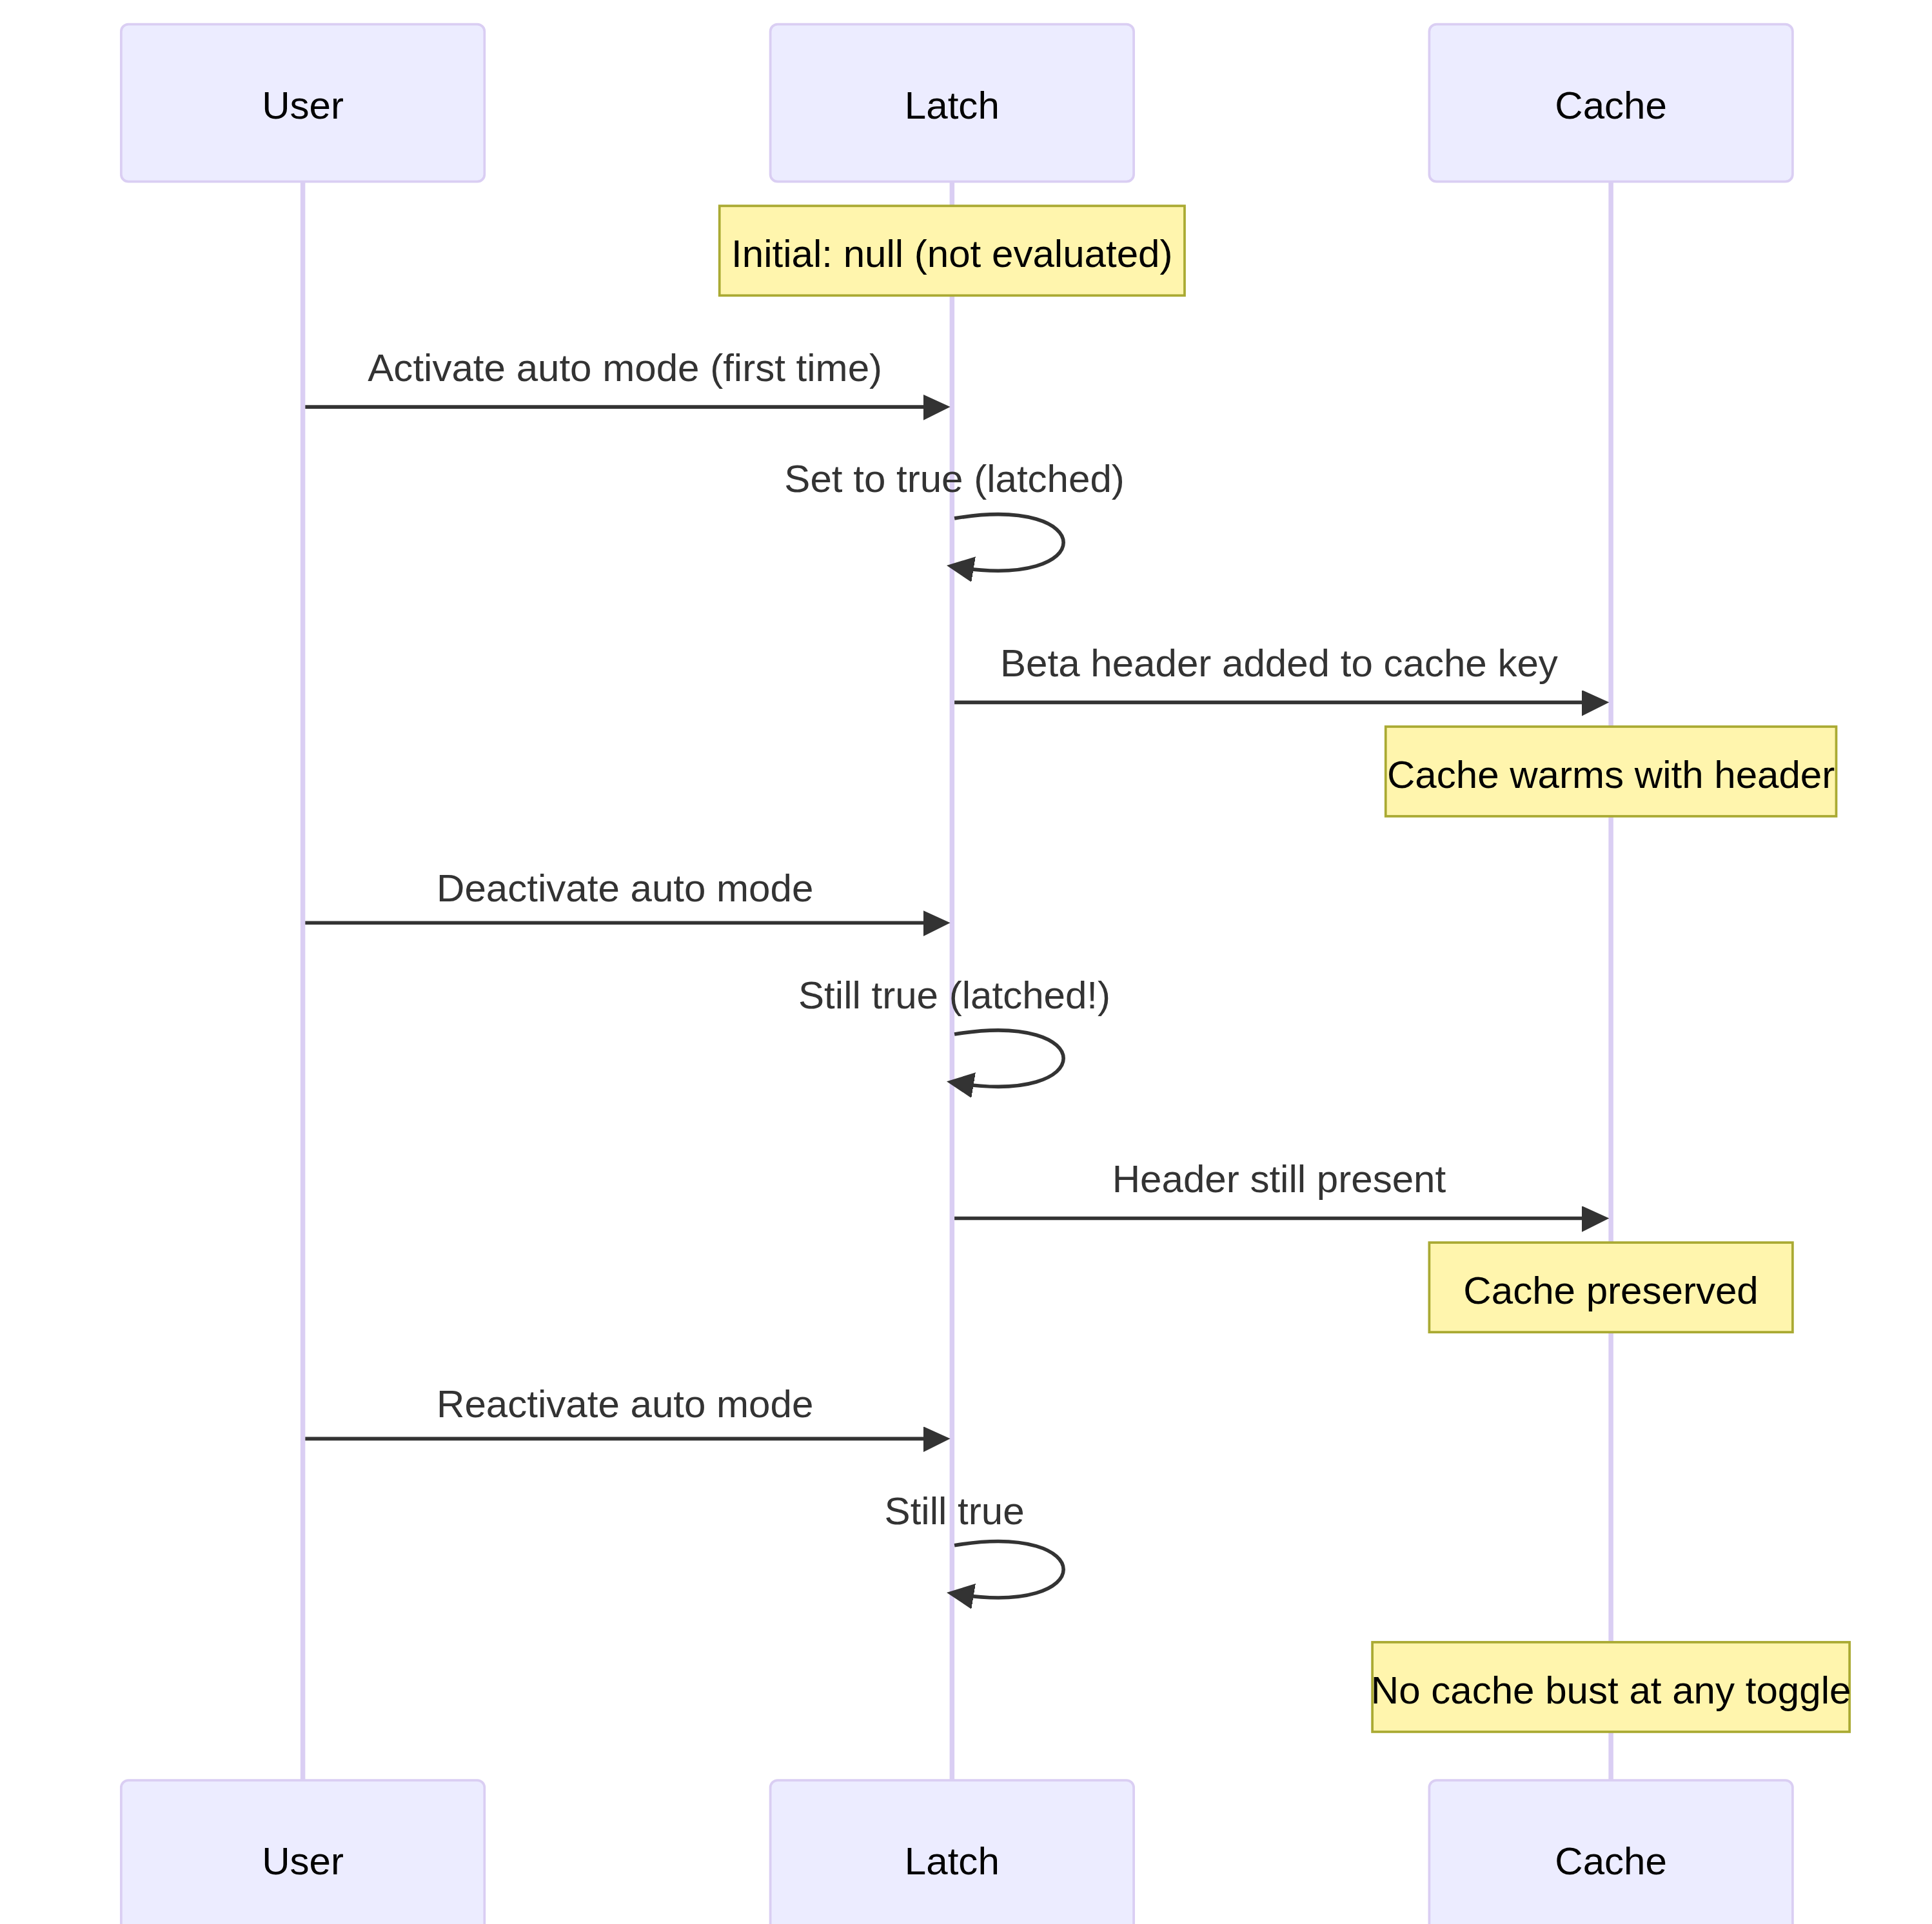
\includegraphics[width=8.47in,height=8.45in]{book/ch03-state_files/figure-latex/mermaid-figure-1.png}

Claude's API supports server-side prompt caching. When consecutive
requests share the same system prompt prefix, the server reuses cached
computations. But the cache key includes HTTP headers and request body
fields. If a beta header appears in request N but not request N+1, the
cache is busted -- even if the prompt content is identical. For a system
prompt exceeding 50,000 tokens, a cache miss is expensive.

The five latches:

\begin{longtable}[]{@{}
  >{\raggedright\arraybackslash}p{(\linewidth - 2\tabcolsep) * \real{0.2917}}
  >{\raggedright\arraybackslash}p{(\linewidth - 2\tabcolsep) * \real{0.7083}}@{}}
\toprule\noalign{}
\begin{minipage}[b]{\linewidth}\raggedright
Latch
\end{minipage} & \begin{minipage}[b]{\linewidth}\raggedright
What It Prevents
\end{minipage} \\
\midrule\noalign{}
\endhead
\bottomrule\noalign{}
\endlastfoot
\texttt{afkModeHeaderLatched} & Shift+Tab auto mode toggling flips the
AFK beta header on/off \\
\texttt{fastModeHeaderLatched} & Fast mode cooldown enter/exit flips the
fast mode header \\
\texttt{cacheEditingHeaderLatched} & Remote feature flag changes bust
every active user's cache \\
\texttt{thinkingClearLatched} & Triggered on confirmed cache miss
(\textgreater1h idle). Prevents re-enabling thinking blocks from busting
freshly warmed cache \\
\texttt{pendingPostCompaction} & Consume-once flag for telemetry:
distinguishes compaction-induced cache misses from TTL-expiry misses \\
\end{longtable}

All five use a three-state type: \texttt{boolean\ \textbar{}\ null}. The
\texttt{null} initial value means ``not yet evaluated.'' \texttt{true}
means ``latched on.'' They never return to \texttt{null} or
\texttt{false} once set to \texttt{true}. This is the defining property
of a latch.

The implementation pattern:

\begin{Shaded}
\begin{Highlighting}[]
\KeywordTok{function} \FunctionTok{shouldSendBetaHeader}\NormalTok{(featureCurrentlyActive}\OperatorTok{:} \DataTypeTok{boolean}\NormalTok{)}\OperatorTok{:} \DataTypeTok{boolean}\NormalTok{ \{}
  \KeywordTok{const}\NormalTok{ latched }\OperatorTok{=} \FunctionTok{getAfkModeHeaderLatched}\NormalTok{()}
  \ControlFlowTok{if}\NormalTok{ (latched }\OperatorTok{===} \KeywordTok{true}\NormalTok{) }\ControlFlowTok{return} \KeywordTok{true}       \CommentTok{// Already latched {-}{-} always send}
  \ControlFlowTok{if}\NormalTok{ (featureCurrentlyActive) \{}
    \FunctionTok{setAfkModeHeaderLatched}\NormalTok{(}\KeywordTok{true}\NormalTok{)          }\CommentTok{// First activation {-}{-} latch it}
    \ControlFlowTok{return} \KeywordTok{true}
\NormalTok{  \}}
  \ControlFlowTok{return} \KeywordTok{false}                             \CommentTok{// Never activated {-}{-} don\textquotesingle{}t send}
\NormalTok{\}}
\end{Highlighting}
\end{Shaded}

Why not just always send all beta headers? Because headers are part of
the cache key. Sending an unrecognized header creates a different cache
namespace. The latch ensures you only enter a cache namespace when you
actually need it, then stay there.

\begin{center}\rule{0.5\linewidth}{0.5pt}\end{center}

\section{3.2 AppState -- The Reactive
Store}\label{appstate-the-reactive-store}

\subsection{The 34-Line
Implementation}\label{the-34-line-implementation}

The UI state store lives in \texttt{state/store.ts}:

The store implementation is approximately 30 lines: a closure over a
\texttt{state} variable, an \texttt{Object.is} equality check to prevent
spurious updates, synchronous listener notification, and an
\texttt{onChange} callback for side effects. The skeleton looks like:

\begin{Shaded}
\begin{Highlighting}[]
\CommentTok{// Pseudocode — illustrates the pattern}
\KeywordTok{function} \FunctionTok{makeStore}\NormalTok{(initial}\OperatorTok{,}\NormalTok{ onTransition) \{}
  \KeywordTok{let}\NormalTok{ current }\OperatorTok{=}\NormalTok{ initial}
  \KeywordTok{const}\NormalTok{ subs }\OperatorTok{=} \KeywordTok{new} \BuiltInTok{Set}\NormalTok{()}
  \ControlFlowTok{return}\NormalTok{ \{}
\NormalTok{    read}\OperatorTok{:}\NormalTok{      () }\KeywordTok{=\textgreater{}}\NormalTok{ current}\OperatorTok{,}
\NormalTok{    update}\OperatorTok{:}\NormalTok{    (fn) }\KeywordTok{=\textgreater{}}\NormalTok{ \{ }\CommentTok{/* Object.is guard, then notify */}\NormalTok{ \}}\OperatorTok{,}
\NormalTok{    subscribe}\OperatorTok{:}\NormalTok{ (cb) }\KeywordTok{=\textgreater{}}\NormalTok{ \{ subs}\OperatorTok{.}\FunctionTok{add}\NormalTok{(cb)}\OperatorTok{;} \ControlFlowTok{return}\NormalTok{ () }\KeywordTok{=\textgreater{}}\NormalTok{ subs}\OperatorTok{.}\FunctionTok{delete}\NormalTok{(cb) \}}\OperatorTok{,}
\NormalTok{  \}}
\NormalTok{\}}
\end{Highlighting}
\end{Shaded}

Thirty-four lines. No middleware, no devtools, no time-travel debugging,
no action types. Just a closure over a mutable variable, a Set of
listeners, and an \texttt{Object.is} equality check. This is Zustand
without the library.

The design decisions worth examining:

\textbf{Updater function pattern.} There is no
\texttt{setState(newValue)} -- only
\texttt{setState((prev)\ =\textgreater{}\ next)}. Every mutation
receives the current state and must produce the next state, eliminating
stale-state bugs from concurrent mutations.

\textbf{\texttt{Object.is} equality check.} If the updater returns the
same reference, the mutation is a no-op. No listeners fire. No side
effects run. Critical for performance -- components that spread-and-set
without changing values produce no re-renders.

\textbf{\texttt{onChange} fires before listeners.} The optional
\texttt{onChange} callback receives both old and new state and fires
synchronously before any subscriber is notified. This is used for side
effects (Section 3.4) that must complete before the UI re-renders.

\textbf{No middleware, no devtools.} This is not an oversight. When your
store needs exactly three operations (get, set, subscribe), an
\texttt{Object.is} equality check, and a synchronous \texttt{onChange}
hook, 34 lines of code you own is better than a dependency. You control
the exact semantics. You can read the entire implementation in thirty
seconds.

\subsection{The AppState Type}\label{the-appstate-type}

The \texttt{AppState} type (\textasciitilde452 lines) is the shape of
everything the UI needs to render. It is wrapped in
\texttt{DeepImmutable\textless{}\textgreater{}} for most fields, with
explicit exclusions for fields containing function types:

\begin{Shaded}
\begin{Highlighting}[]
\ImportTok{export type}\NormalTok{ AppState }\OperatorTok{=}\NormalTok{ DeepImmutable}\OperatorTok{\textless{}}\NormalTok{\{}
\NormalTok{  settings}\OperatorTok{:}\NormalTok{ SettingsJson}
\NormalTok{  verbose}\OperatorTok{:} \DataTypeTok{boolean}
  \CommentTok{// ... \textasciitilde{}150 more fields}
\NormalTok{\}}\OperatorTok{\textgreater{}} \OperatorTok{\&}\NormalTok{ \{}
\NormalTok{  tasks}\OperatorTok{:}\NormalTok{ \{ [taskId}\OperatorTok{:} \DataTypeTok{string}\NormalTok{]}\OperatorTok{:}\NormalTok{ TaskState \}  }\CommentTok{// Contains abort controllers}
\NormalTok{  agentNameRegistry}\OperatorTok{:} \BuiltInTok{Map}\OperatorTok{\textless{}}\DataTypeTok{string}\OperatorTok{,}\NormalTok{ AgentId}\OperatorTok{\textgreater{}}
\NormalTok{\}}
\end{Highlighting}
\end{Shaded}

The intersection type lets most fields be deeply immutable while
exempting fields that hold functions, Maps, and mutable refs. Full
immutability is the default, with surgical escape hatches where the type
system would fight the runtime semantics.

\subsection{React Integration}\label{react-integration}

The store integrates with React through \texttt{useSyncExternalStore}:

\begin{Shaded}
\begin{Highlighting}[]
\CommentTok{// Standard React pattern — useSyncExternalStore with a selector}
\ImportTok{export} \KeywordTok{function} \FunctionTok{useAppState}\OperatorTok{\textless{}}\NormalTok{T}\OperatorTok{\textgreater{}}\NormalTok{(selector}\OperatorTok{:}\NormalTok{ (state}\OperatorTok{:}\NormalTok{ AppState) }\KeywordTok{=\textgreater{}}\NormalTok{ T)}\OperatorTok{:}\NormalTok{ T \{}
  \KeywordTok{const}\NormalTok{ store }\OperatorTok{=} \FunctionTok{useContext}\NormalTok{(AppStoreContext)}
  \ControlFlowTok{return} \FunctionTok{useSyncExternalStore}\NormalTok{(}
\NormalTok{    store}\OperatorTok{.}\AttributeTok{subscribe}\OperatorTok{,}
\NormalTok{    () }\KeywordTok{=\textgreater{}} \FunctionTok{selector}\NormalTok{(store}\OperatorTok{.}\FunctionTok{getState}\NormalTok{())}\OperatorTok{,}
\NormalTok{  )}
\NormalTok{\}}
\end{Highlighting}
\end{Shaded}

The selector must return an existing sub-object reference (not a freshly
constructed object) for \texttt{Object.is} comparison to prevent
unnecessary re-renders. If you write
\texttt{useAppState(s\ =\textgreater{}\ (\{\ a:\ s.a,\ b:\ s.b\ \}))},
every render produces a new object reference, and the component
re-renders on every state change. This is the same constraint Zustand
users face -- cheaper comparisons, but the selector author must
understand reference identity.

\begin{center}\rule{0.5\linewidth}{0.5pt}\end{center}

\section{3.3 How the Two Tiers Relate}\label{how-the-two-tiers-relate}

The two tiers communicate through explicit, narrow interfaces.

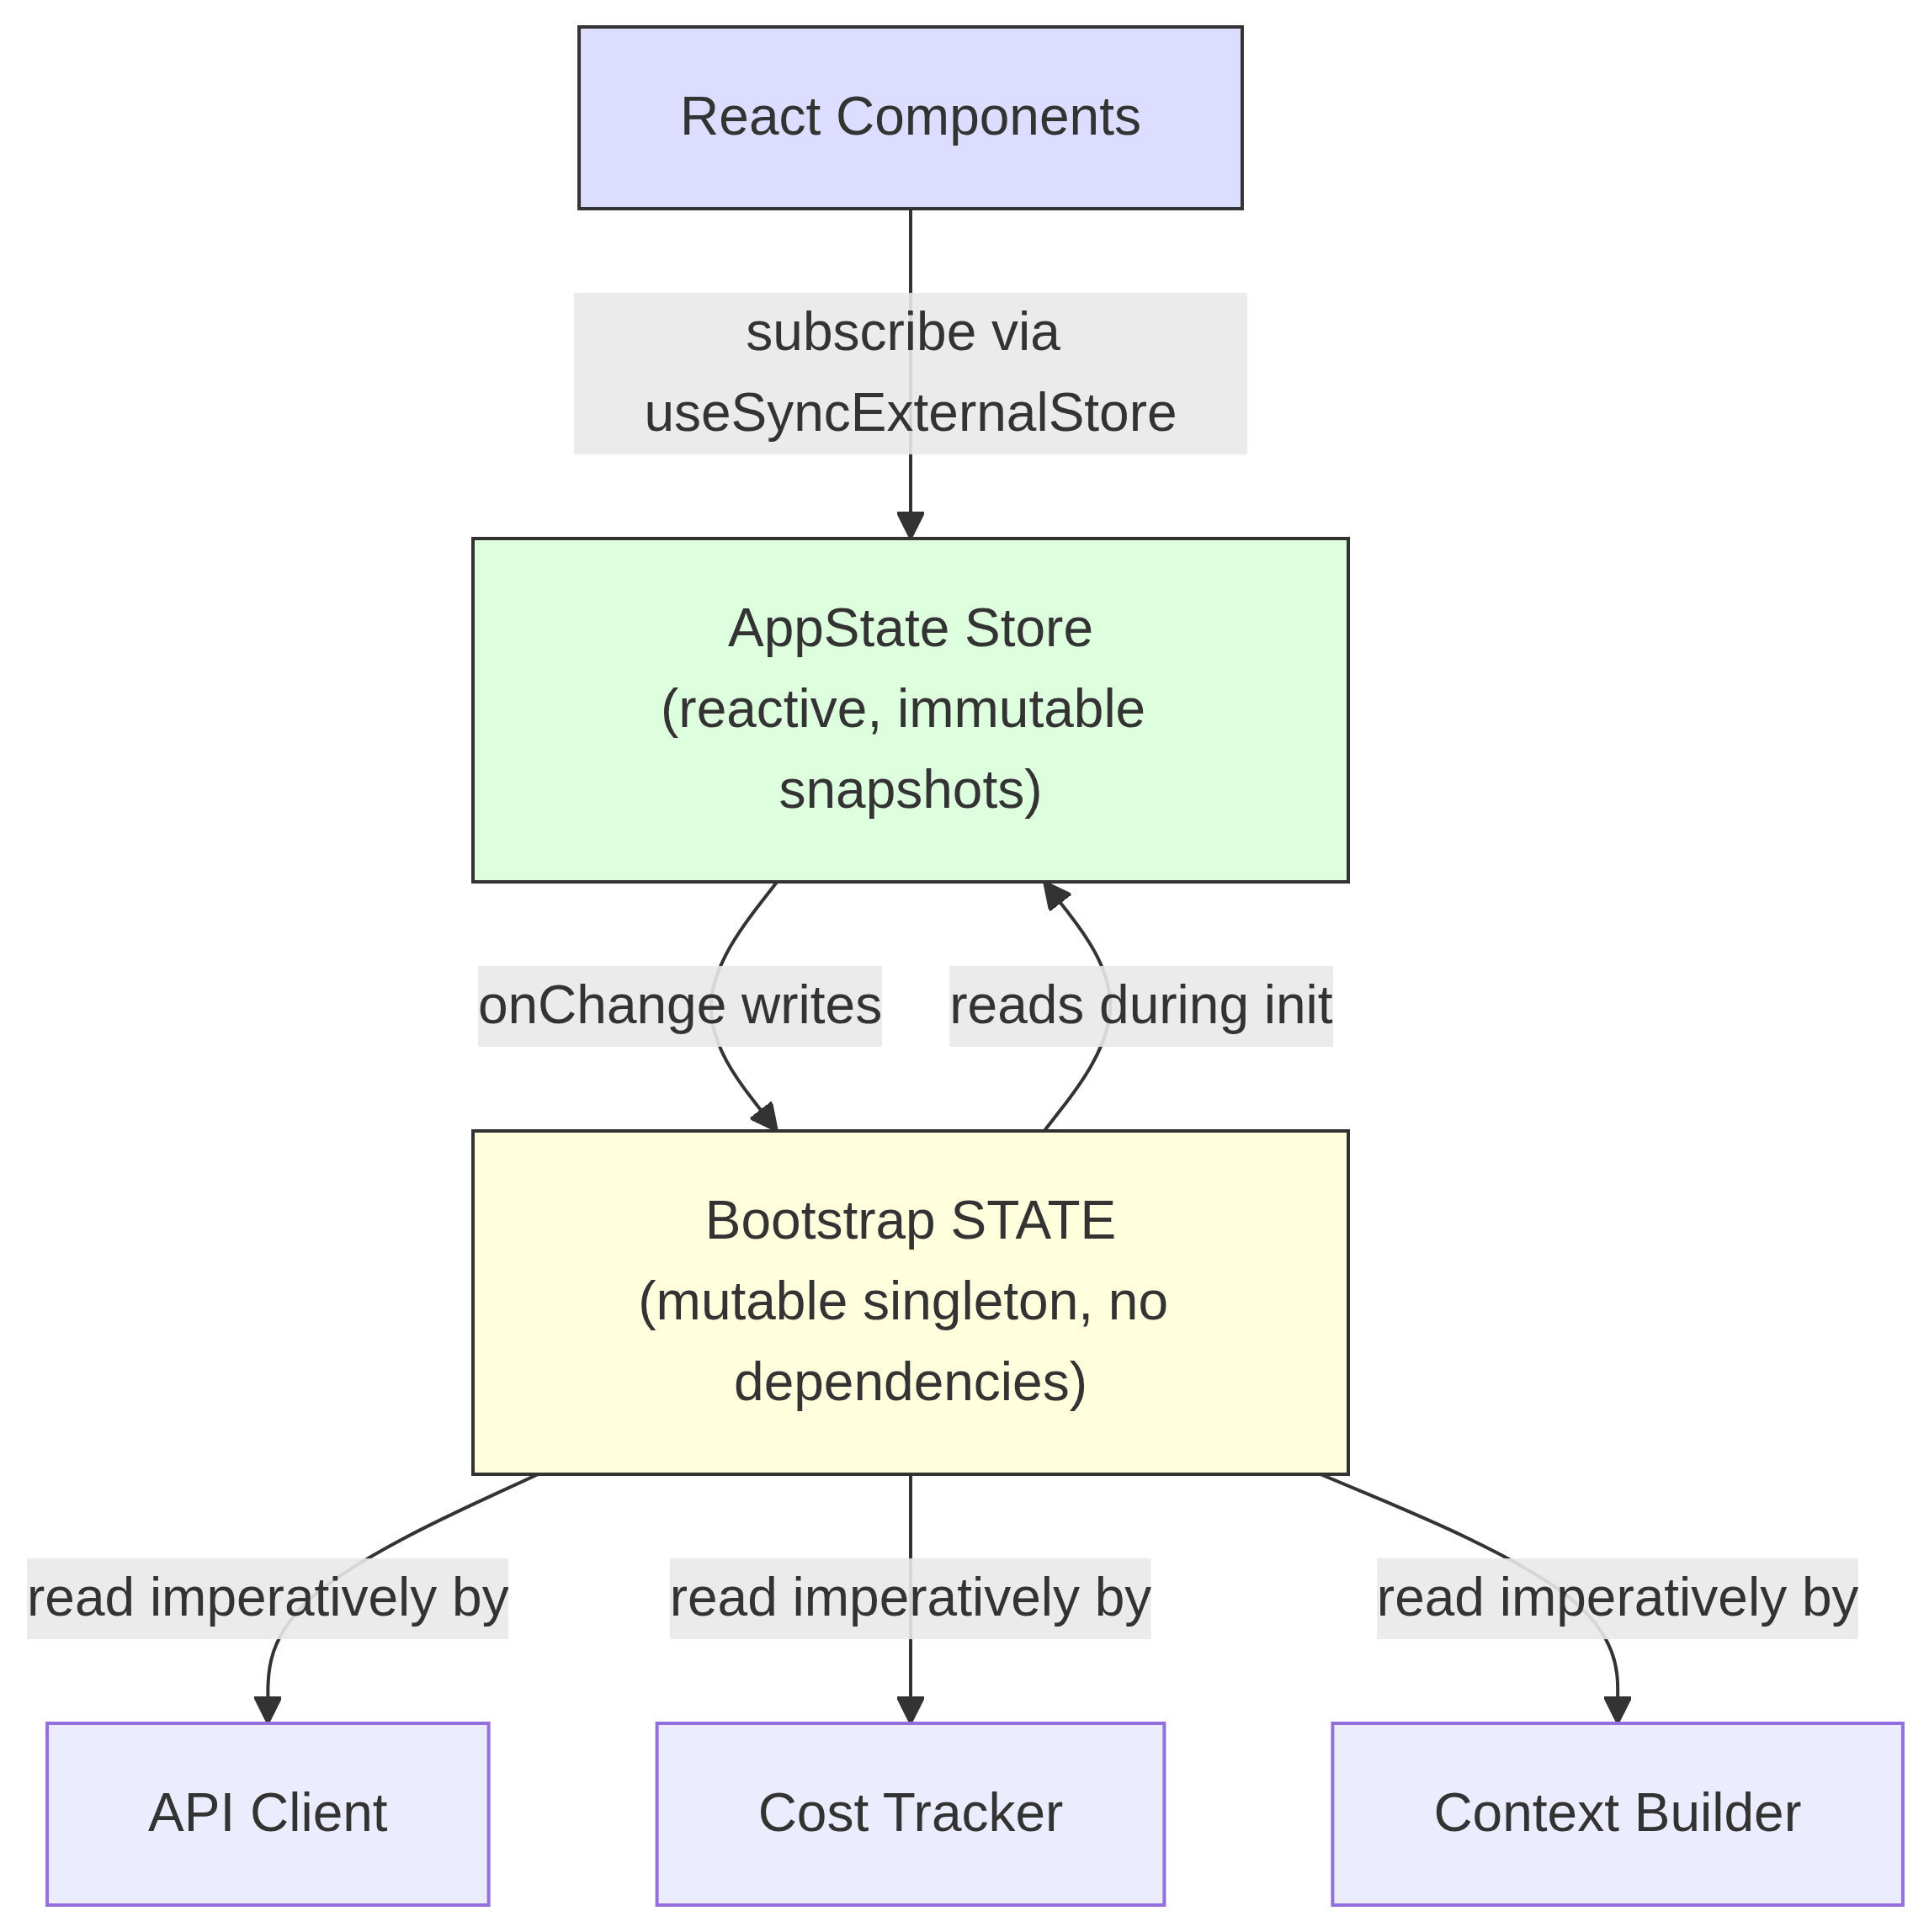
\includegraphics[width=5.97in,height=5.98in]{book/ch03-state_files/figure-latex/mermaid-figure-2.png}

Bootstrap state flows into AppState during initialization:
\texttt{getDefaultAppState()} reads settings from disk (which bootstrap
helped locate), checks feature flags (which bootstrap evaluated), and
sets the initial model (which bootstrap resolved from CLI args and
settings).

AppState flows back to bootstrap state through side effects: when the
user changes the model, \texttt{onChangeAppState} calls
\texttt{setMainLoopModelOverride()} in bootstrap. When settings change,
credential caches in bootstrap are cleared.

But the two tiers never share a reference. A module that imports
bootstrap state does not need to know about React. A component that
reads AppState does not need to know about the process singleton.

A concrete example clarifies the data flow. When the user types
\texttt{/model\ claude-sonnet-4}:

\begin{enumerate}
\def\labelenumi{\arabic{enumi}.}
\tightlist
\item
  The command handler calls
  \texttt{store.setState(prev\ =\textgreater{}\ (\{\ ...prev,\ mainLoopModel:\ \textquotesingle{}claude-sonnet-4\textquotesingle{}\ \}))}
\item
  The store's \texttt{Object.is} check detects a change
\item
  \texttt{onChangeAppState} fires, detects the model changed, calls
  \texttt{setMainLoopModelOverride()} (updates bootstrap) and
  \texttt{updateSettingsForSource()} (persists to disk)
\item
  All store subscribers fire -- React components re-render to show the
  new model name
\item
  The next API call reads the model from
  \texttt{getMainLoopModelOverride()} in bootstrap state
\end{enumerate}

Steps 1-4 are synchronous. The API client in step 5 may run seconds
later. But it reads from bootstrap state (updated in step 3), not from
AppState. This is the two-tier handoff: the UI store is the source of
truth for what the user chose, but bootstrap state is the source of
truth for what the API client uses.

The DAG property -- bootstrap depends on nothing, AppState depends on
bootstrap for init, React depends on AppState -- is enforced by an
ESLint rule that prevents \texttt{bootstrap/state.ts} from importing
modules outside its allowed set.

\begin{center}\rule{0.5\linewidth}{0.5pt}\end{center}

\section{3.4 Side Effects:
onChangeAppState}\label{side-effects-onchangeappstate}

The \texttt{onChange} callback is where the two tiers synchronize. Every
\texttt{setState} call triggers \texttt{onChangeAppState}, which
receives both previous and new state and decides what external effects
to fire.

\textbf{Permission mode sync} is the primary use case. Prior to this
centralized handler, permission mode was synced to the remote session
(CCR) by only 2 of 8+ mutation paths. The other six -- Shift+Tab
cycling, dialog options, slash commands, rewind, bridge callbacks -- all
mutated AppState without telling CCR. The external metadata drifted out
of sync.

The fix: stop scattering notifications across mutation sites and instead
hook the diff in one place. The comment in the source code lists every
mutation path that was broken and notes that ``the scattered callsites
above need zero changes.'' This is the architectural benefit of
centralized side effects -- coverage is structural, not manual.

\textbf{Model changes} keep bootstrap state in sync with what the UI
renders. \textbf{Settings changes} clear credential caches and re-apply
environment variables. \textbf{Verbose toggle} and \textbf{expanded
view} are persisted to global config.

The pattern -- centralized side effects on a diffable state transition
-- is essentially the Observer pattern applied at the granularity of a
state diff rather than individual events. It scales better than
scattered event emissions because the number of side effects grows much
more slowly than the number of mutation sites.

\begin{center}\rule{0.5\linewidth}{0.5pt}\end{center}

\section{3.5 Context Building}\label{context-building}

Three memoized async functions in \texttt{context.ts} build the system
prompt context prepended to every conversation. Each is computed once
per session, not per turn.

\texttt{getGitStatus} runs five git commands in parallel
(\texttt{Promise.all}), producing a block with the current branch,
default branch, recent commits, and working tree status. The
\texttt{-\/-no-optional-locks} flag prevents git from taking write locks
that could interfere with concurrent git operations in another terminal.

\texttt{getUserContext} loads CLAUDE.md content and caches it in
bootstrap state via \texttt{setCachedClaudeMdContent}. This cache breaks
a circular dependency: the auto-mode classifier needs CLAUDE.md content,
but CLAUDE.md loading goes through the filesystem, which goes through
permissions, which calls the classifier. By caching in bootstrap state
(a DAG leaf), the cycle is broken.

All three context functions use Lodash's \texttt{memoize} (compute once,
cache forever) rather than TTL-based caching. The reasoning: if git
status were re-computed every 5 minutes, the change would bust the
server-side prompt cache. The system prompt even tells the model: ``This
is the git status at the start of the conversation. Note that this
status is a snapshot in time.''

\begin{center}\rule{0.5\linewidth}{0.5pt}\end{center}

\section{3.6 Cost Tracking}\label{cost-tracking}

Every API response flows through \texttt{addToTotalSessionCost}, which
accumulates per-model usage, updates bootstrap state, reports to
OpenTelemetry, and recursively processes advisor tool usage (nested
model calls within a response).

Cost state survives process restarts through save-and-restore to a
project config file. The session ID is used as a guard -- costs are only
restored if the persisted session ID matches the session being resumed.

Histograms use reservoir sampling (Algorithm R) to maintain bounded
memory while accurately representing distributions. The 1,024-entry
reservoir produces p50, p95, and p99 percentiles. Why not a simple
running average? Because averages hide distribution shape. A session
where 95\% of API calls take 200ms and 5\% take 10 seconds has the same
average as one where all calls take 690ms, but the user experience is
radically different.

\begin{center}\rule{0.5\linewidth}{0.5pt}\end{center}

\section{3.7 What We Learned}\label{what-we-learned}

The codebase has grown from a simple CLI to a system with
\textasciitilde450 lines of state type definitions, \textasciitilde80
fields of process state, a side-effect system, multiple persistence
boundaries, and cache optimization latches. None of this was designed
upfront. The sticky latches were added when cache busting became a
measurable cost problem. The \texttt{onChange} handler was centralized
when 6 of 8 permission sync paths were discovered to be broken. The
CLAUDE.md cache was added when a circular dependency emerged.

This is the natural growth pattern of state in a complex application.
The two-tier architecture provides enough structure to contain the
growth -- new bootstrap fields do not affect React rendering, new
AppState fields do not create import cycles -- while remaining flexible
enough to accommodate patterns that were not anticipated in the original
design.

\begin{center}\rule{0.5\linewidth}{0.5pt}\end{center}

\section{3.8 State Architecture
Summary}\label{state-architecture-summary}

\begin{longtable}[]{@{}
  >{\raggedright\arraybackslash}p{(\linewidth - 4\tabcolsep) * \real{0.3333}}
  >{\raggedright\arraybackslash}p{(\linewidth - 4\tabcolsep) * \real{0.3333}}
  >{\raggedright\arraybackslash}p{(\linewidth - 4\tabcolsep) * \real{0.3333}}@{}}
\toprule\noalign{}
\begin{minipage}[b]{\linewidth}\raggedright
Property
\end{minipage} & \begin{minipage}[b]{\linewidth}\raggedright
Bootstrap State
\end{minipage} & \begin{minipage}[b]{\linewidth}\raggedright
AppState
\end{minipage} \\
\midrule\noalign{}
\endhead
\bottomrule\noalign{}
\endlastfoot
\textbf{Location} & Module-scope singleton & React context \\
\textbf{Mutability} & Mutable through setters & Immutable snapshots via
updater \\
\textbf{Subscribers} & Signal (pub/sub) for specific events &
\texttt{useSyncExternalStore} for React \\
\textbf{Availability} & Import time (before React) & After provider
mounts \\
\textbf{Persistence} & Process exit handlers & Via onChange to disk \\
\textbf{Equality} & N/A (imperative reads) & \texttt{Object.is}
reference check \\
\textbf{Dependencies} & DAG leaf (imports nothing) & Imports types from
across codebase \\
\textbf{Test reset} & \texttt{resetStateForTests()} & Create new store
instance \\
\textbf{Primary consumers} & API client, cost tracker, context builder &
React components, side effects \\
\end{longtable}

\begin{center}\rule{0.5\linewidth}{0.5pt}\end{center}

\section{Apply This}\label{apply-this-2}

\textbf{Separate state by access pattern, not by domain.} Session ID
belongs in the singleton not because it is ``infrastructure'' in the
abstract, but because it must be readable before React mounts and
writable without notifying subscribers. Permission mode belongs in the
reactive store because changing it must trigger re-renders and side
effects. Let the access pattern drive the tier, and the architecture
follows naturally.

\textbf{The sticky latch pattern.} Any system that interacts with a
cache (prompt cache, CDN, query cache) faces the same problem: feature
toggles that change the cache key mid-session cause invalidation. Once a
feature is activated, its cache key contribution stays active for the
session. The three-state type (\texttt{boolean\ \textbar{}\ null},
meaning ``not evaluated / on / never off'') makes the intent
self-documenting. Especially valuable when the cache is not under your
control.

\textbf{Centralize side effects on state diffs.} When multiple code
paths can change the same state, do not scatter notifications across
mutation sites. Hook the store's \texttt{onChange} callback and detect
which fields changed. Coverage becomes structural (any mutation triggers
the effect) rather than manual (each mutation site must remember to
notify).

\textbf{Prefer 34 lines you own over a library you do not.} When your
requirements are exactly get, set, subscribe, and a change callback, a
minimal implementation gives you full control over the semantics. In a
system where state management bugs can cost real money, that
transparency has value. The key insight is recognizing when you do
\emph{not} need a library.

\textbf{Use process exit as a persistence boundary with intention.}
Multiple subsystems persist state on process exit. The trade-off is
explicit: non-graceful termination (SIGKILL, OOM) loses accumulated
data. This is acceptable because the data is diagnostic, not
transactional, and writing to disk on every state change would be too
expensive for counters that increment hundreds of times per session.

\begin{center}\rule{0.5\linewidth}{0.5pt}\end{center}

The two-tier architecture established in this chapter -- bootstrap
singleton for infrastructure, reactive store for UI, side effects
bridging them -- is the foundation that every subsequent chapter builds
on. The conversation loop (Chapter 4) reads context from the memoized
builders. The tool system (Chapter 5) checks permissions from AppState.
The agent system (Chapter 8) creates task entries in AppState while
tracking costs in bootstrap state. Understanding where state lives, and
why, is prerequisite to understanding how any of these systems work.

Some fields straddle the boundary. The main loop model exists in both
tiers: \texttt{mainLoopModel} in AppState (for UI rendering) and
\texttt{mainLoopModelOverride} in bootstrap state (for API client
consumption). The \texttt{onChangeAppState} handler keeps them
synchronized. This duplication is the cost of the two-tier split. But
the alternative -- having the API client import the React store, or
having React components read from the process singleton -- would violate
the dependency direction that keeps the architecture sound. A small
amount of controlled duplication, bridged by a centralized
synchronization point, is preferable to a tangled dependency graph.

\chapter{Chapter 4: Talking to Claude -- The API
Layer}\label{chapter-4-talking-to-claude-the-api-layer}

Chapter 3 established where state lives and how the two tiers
communicate. Now we follow what happens when that state is put to use:
the system needs to talk to a language model. Everything in Claude Code
-- the bootstrap sequence, the state system, the permission framework --
exists to serve this moment.

This layer handles more failure modes than any other part of the system.
It must route through four cloud providers via a single transparent
interface. It must construct system prompts with byte-level awareness of
how the server's prompt cache works, because a single misplaced section
can bust a cache worth 50,000+ tokens. It must stream responses with
active failure detection, because TCP connections die silently. And it
must maintain session-stable invariants so that mid-conversation changes
to feature flags do not cause invisible performance cliffs.

Let us trace a single API call from start to finish.

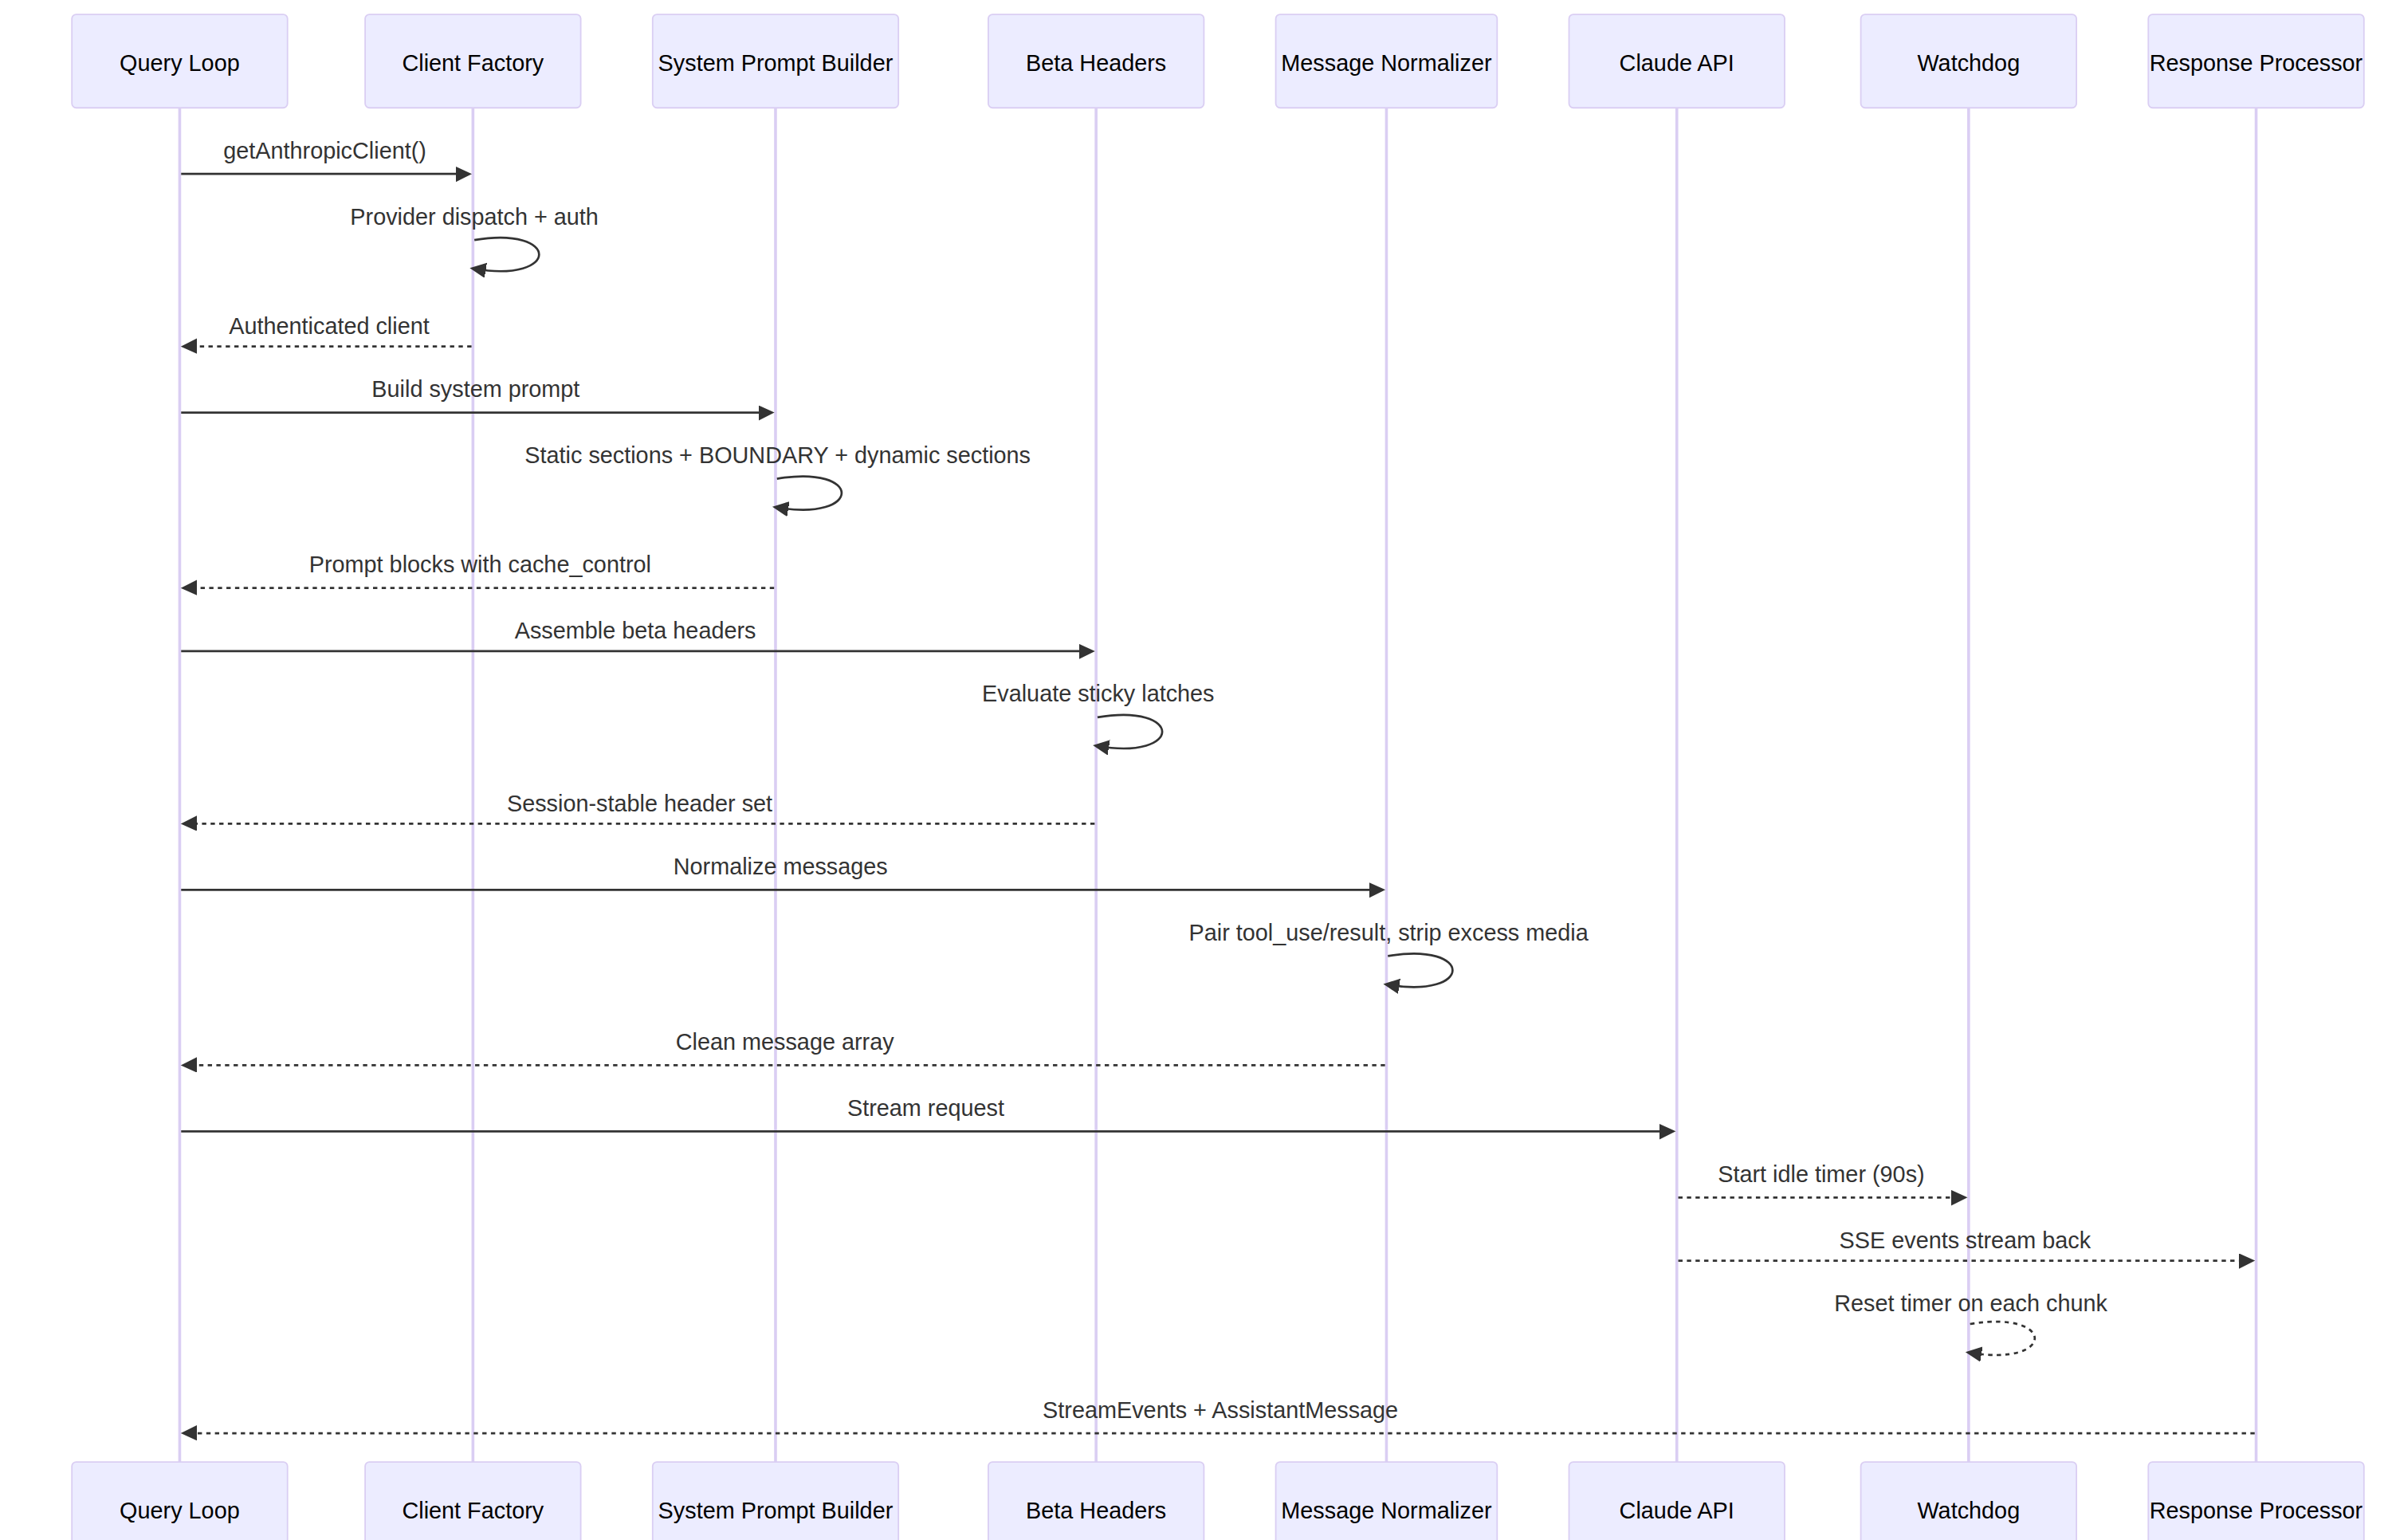
\includegraphics[width=17.65in,height=11.39in]{book/ch04-api-layer_files/figure-latex/mermaid-figure-1.png}

\begin{center}\rule{0.5\linewidth}{0.5pt}\end{center}

\section{The Multi-Provider Client
Factory}\label{the-multi-provider-client-factory}

The \texttt{getAnthropicClient()} function is the single factory for all
model communication. It returns an Anthropic SDK client configured for
whichever provider the deployment targets:

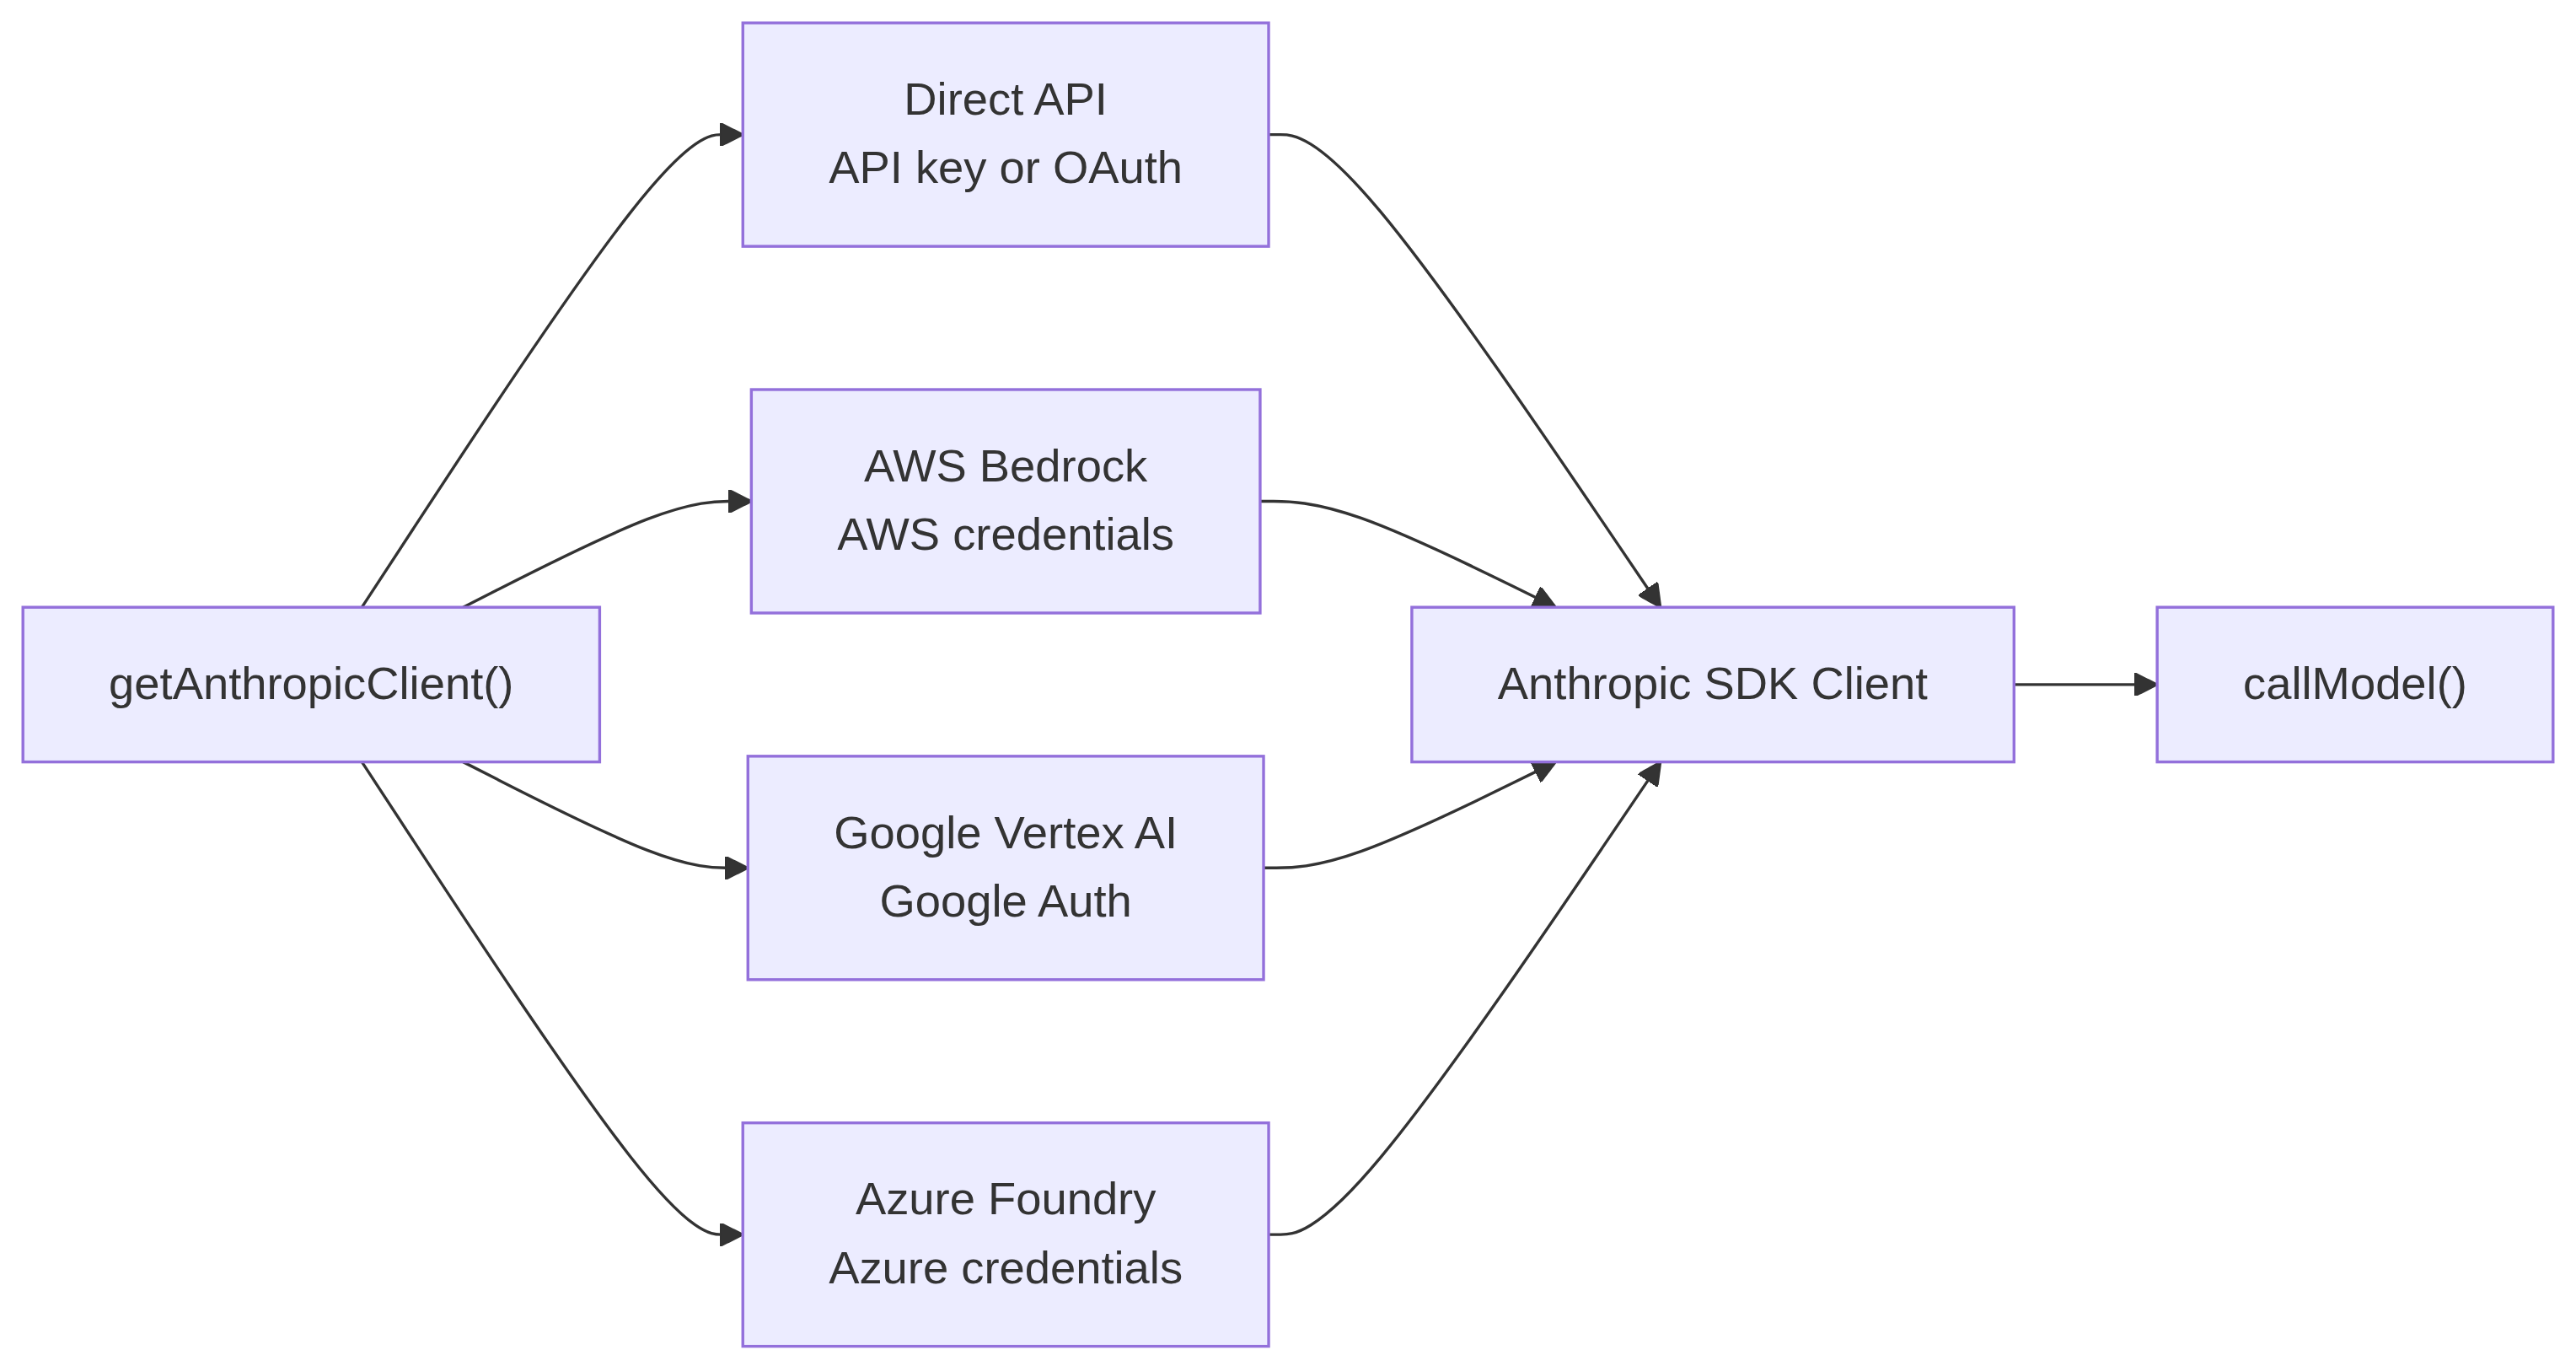
\includegraphics[width=9.37in,height=4.98in]{book/ch04-api-layer_files/figure-latex/mermaid-figure-3.png}

The dispatch is entirely environment-variable driven, evaluated in a
fixed priority order. All four provider-specific SDK classes are cast to
\texttt{Anthropic} via \texttt{as\ unknown\ as\ Anthropic}. The comment
in the source is refreshingly honest: ``we have always been lying about
the return type.'' This deliberate type erasure means every consumer
sees a uniform interface. The rest of the codebase never branches on
provider.

Each provider SDK is dynamically imported -- \texttt{AnthropicBedrock},
\texttt{AnthropicFoundry}, \texttt{AnthropicVertex} are heavy modules
with their own dependency trees. The dynamic import ensures unused
providers never load.

Provider selection is determined at startup and stored in bootstrap
\texttt{STATE}. The query loop never checks which provider is active.
Switching from Direct API to Bedrock is a configuration change, not a
code change.

\subsection{The buildFetch Wrapper}\label{the-buildfetch-wrapper}

Every outbound fetch gets wrapped to inject an
\texttt{x-client-request-id} header -- a UUID generated per request.
When a request times out, the server never assigns a request ID to the
response. Without the client-side ID, the API team cannot correlate the
timeout with server-side logs. This header bridges that gap. It is only
sent to first-party Anthropic endpoints -- third-party providers might
reject unknown headers.

\begin{center}\rule{0.5\linewidth}{0.5pt}\end{center}

\section{System Prompt Construction}\label{system-prompt-construction}

The system prompt is the most cache-sensitive artifact in the entire
system. Claude's API provides server-side prompt caching: identical
prompt prefixes across requests can be cached, saving both latency and
cost. A 200K-token conversation might have 50-70K tokens that are
identical to the previous turn. Busting that cache forces the server to
re-process all of it.

\subsection{The Dynamic Boundary
Marker}\label{the-dynamic-boundary-marker}

The prompt is built as an array of string sections with a critical
dividing line:

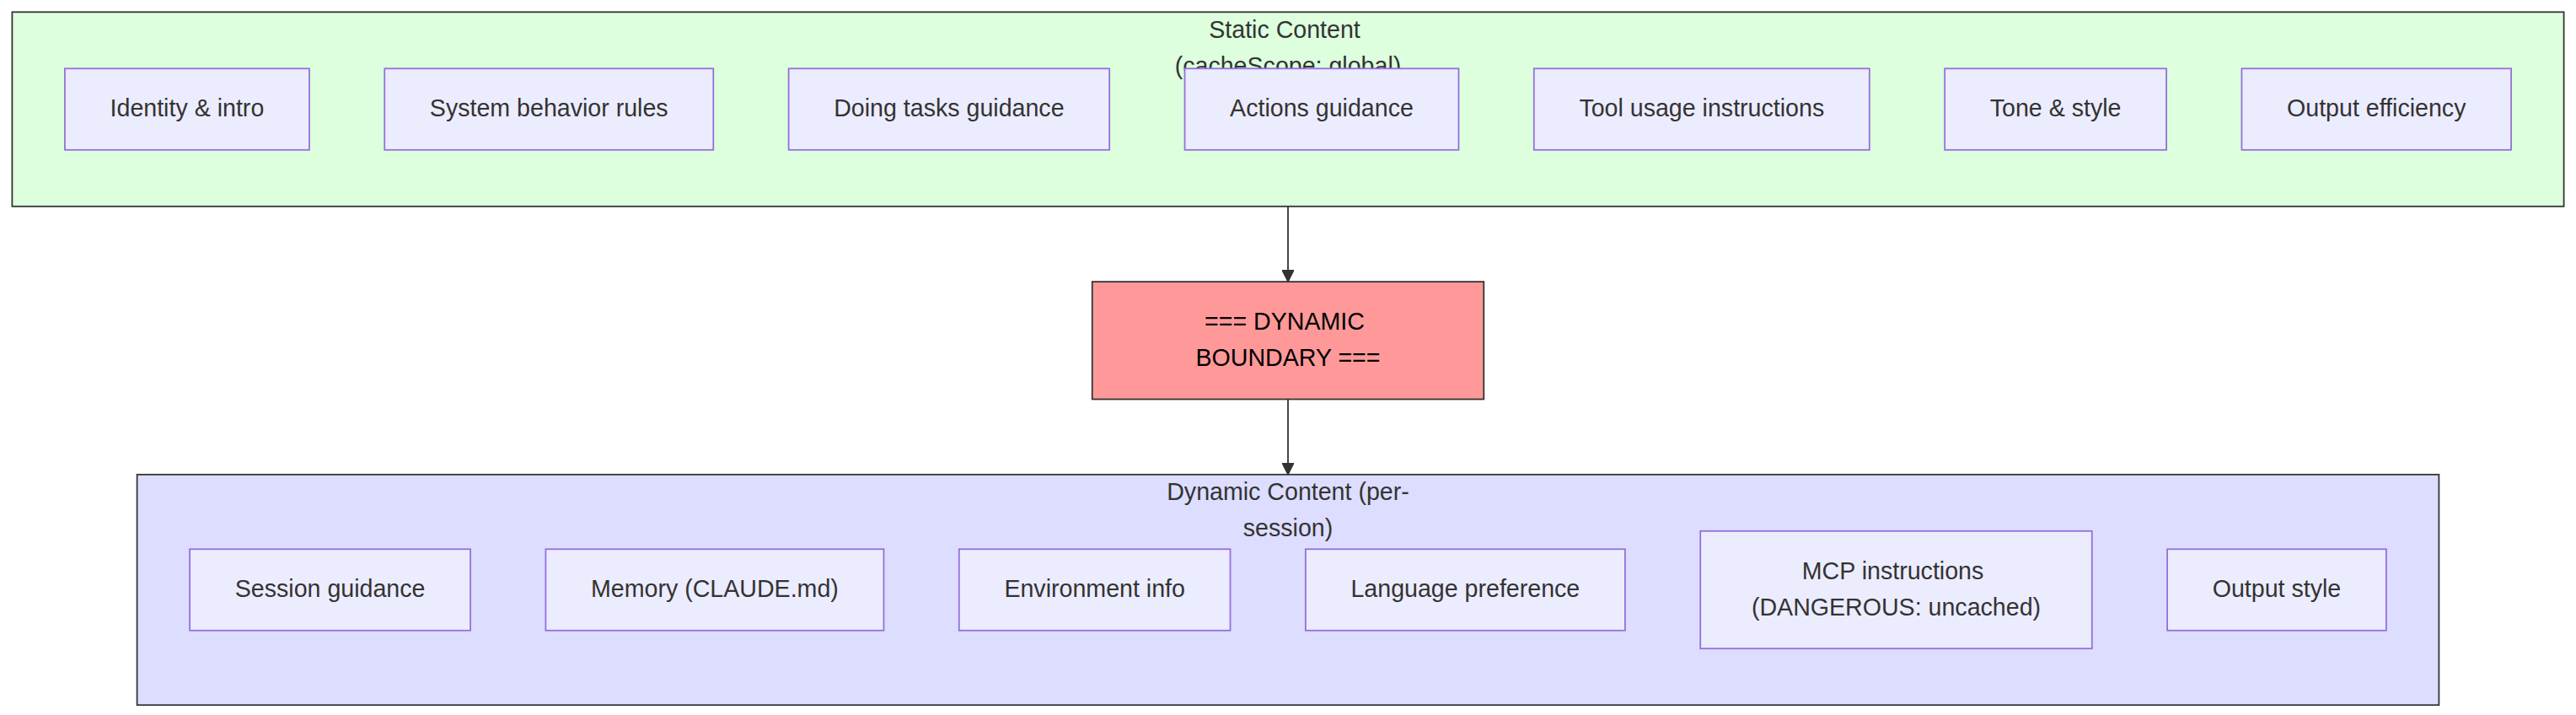
\includegraphics[width=17.81in,height=4.96in]{book/ch04-api-layer_files/figure-latex/mermaid-figure-2.png}

Everything before the boundary is identical across sessions, users, and
organizations -- it gets the highest tier of server-side caching.
Everything after contains user-specific content and drops to per-session
caching.

The naming convention for sections is deliberately loud. Adding a new
section requires choosing between \texttt{systemPromptSection} (safe,
cached) and \texttt{DANGEROUS\_uncachedSystemPromptSection}
(cache-breaking, requires a reason string). The \texttt{\_reason}
parameter is unused at runtime but serves as mandatory documentation --
every cache-breaking section carries its justification in the source
code.

\subsection{The 2\^{}N Problem}\label{the-2n-problem}

A comment in \texttt{prompts.ts} explains why conditional sections must
go after the boundary:

\begin{quote}
Each conditional here is a runtime bit that would otherwise multiply the
Blake2b prefix hash variants (2\^{}N).
\end{quote}

Every boolean condition before the boundary doubles the number of unique
global cache entries. Three conditionals create 8 variants; five create
32. The static sections are deliberately unconditional. Compile-time
feature flags (resolved by the bundler) are acceptable before the
boundary. Runtime checks (is this Haiku? does the user have auto mode?)
must go after.

This is the kind of constraint that is invisible until you violate it. A
well-intentioned engineer adding a user-setting-gated section before the
boundary could silently fragment the global cache and double the fleet's
prompt processing costs.

\begin{center}\rule{0.5\linewidth}{0.5pt}\end{center}

\section{Streaming}\label{streaming}

\subsection{Raw SSE Over SDK
Abstractions}\label{raw-sse-over-sdk-abstractions}

The streaming implementation uses the raw
\texttt{Stream\textless{}BetaRawMessageStreamEvent\textgreater{}} rather
than the SDK's higher-level \texttt{BetaMessageStream}. The reason:
\texttt{BetaMessageStream} calls \texttt{partialParse()} on every
\texttt{input\_json\_delta} event. For tool calls with large JSON inputs
(file edits with hundreds of lines), this re-parses the growing JSON
string from scratch on every chunk -- O(n\^{}2) behavior. Claude Code
handles tool input accumulation itself, so the partial parsing is pure
waste.

\subsection{The Idle Watchdog}\label{the-idle-watchdog}

TCP connections can die without notification. The server may crash, a
load balancer may silently drop the connection, or a corporate proxy may
time out. The SDK's request timeout only covers the initial fetch --
once HTTP 200 arrives, the timeout is satisfied. If the streaming body
stops, nothing catches it.

The watchdog: a \texttt{setTimeout} that resets on every received chunk.
If no chunks arrive for 90 seconds, the stream is aborted and the system
falls back to a non-streaming retry. A warning fires at the 45-second
mark. When the watchdog fires, it logs the event with the client request
ID for correlation.

\subsection{Non-Streaming Fallback}\label{non-streaming-fallback}

When streaming fails mid-response (network error, stall, truncation),
the system falls back to a synchronous \texttt{messages.create()} call.
This handles proxy failures where the proxy returns HTTP 200 with a
non-SSE body, or truncates the SSE stream partway through.

The fallback can be disabled when streaming tool execution is active,
since a fallback would re-execute the entire request and potentially run
tools twice.

\begin{center}\rule{0.5\linewidth}{0.5pt}\end{center}

\section{Prompt Cache System}\label{prompt-cache-system}

\subsection{Three Tiers}\label{three-tiers}

Prompt caching operates at three levels:

\textbf{Ephemeral cache} (default): Per-session caching with a
server-defined TTL (\textasciitilde5 minutes). All users get this.

\textbf{1-hour TTL}: Eligible users get extended caching. Eligibility is
determined by subscription status and latched in bootstrap state -- the
\texttt{promptCache1hEligible} sticky latch from Chapter 3 ensures a
mid-session overage flip does not change the TTL.

\textbf{Global scope}: System prompt cache entries get cross-session,
cross-organization sharing. The static portions of the prompt are
identical for all Claude Code users, so a single cached copy serves
everyone. Global scope is disabled when MCP tools are present, because
MCP tool definitions are user-specific and would fragment the cache into
millions of unique prefixes.

\subsection{The Sticky Latches in
Action}\label{the-sticky-latches-in-action}

The five sticky latches from Chapter 3 are evaluated here, during
request construction. Each latch starts as \texttt{null} and, once set
to \texttt{true}, remains \texttt{true} for the session. The comment
above the latch block is precise: ``Sticky-on latches for dynamic beta
headers. Each header, once first sent, keeps being sent for the rest of
the session so mid-session toggles don't change the server-side cache
key and bust \textasciitilde50-70K tokens.''

See Chapter 3, Section 3.1 for the full explanation of the latch
pattern, the five specific latches, and why always-send-all-headers is
not the right solution.

\begin{center}\rule{0.5\linewidth}{0.5pt}\end{center}

\section{The queryModel Generator}\label{the-querymodel-generator}

The \texttt{queryModel()} function is an async generator
(\textasciitilde700 lines) that orchestrates the entire API call
lifecycle. It yields \texttt{StreamEvent}, \texttt{AssistantMessage},
and \texttt{SystemAPIErrorMessage} objects.

The request assembly follows a carefully ordered sequence:

\begin{enumerate}
\def\labelenumi{\arabic{enumi}.}
\tightlist
\item
  \textbf{Kill switch check} -- safety valve for the most expensive
  model tier
\item
  \textbf{Beta header assembly} -- model-specific, with sticky latches
  applied
\item
  \textbf{Tool schema building} -- parallel via \texttt{Promise.all()},
  deferred tools excluded until discovered
\item
  \textbf{Message normalization} -- repair orphaned
  tool\_use/tool\_result mismatches, strip excess media, remove stale
  blocks
\item
  \textbf{System prompt block construction} -- split at the dynamic
  boundary, assign cache scopes
\item
  \textbf{Retry-wrapped streaming} -- handles 529 (overloaded), model
  fallback, thinking downgrade, OAuth refresh
\end{enumerate}

\subsection{Output Token Cap}\label{output-token-cap}

The default output cap is 8,000 tokens, not the typical 32K or 64K.
Production data showed that p99 output is 4,911 tokens -- standard
limits over-reserve by 8-16x. When a response hits the cap (\textless1\%
of requests), it gets one clean retry at 64K. This saves significant
cost at fleet scale.

\subsection{Error Handling and Retry}\label{error-handling-and-retry}

The \texttt{withRetry()} function is itself an async generator that
yields \texttt{SystemAPIErrorMessage} events so the UI can display retry
status. Retry strategies:

\begin{itemize}
\tightlist
\item
  \textbf{529 (overloaded)}: Wait and retry, optionally downgrading fast
  mode
\item
  \textbf{Model fallback}: Primary model fails, try a fallback (e.g.,
  Opus to Sonnet)
\item
  \textbf{Thinking downgrade}: Context window overflow triggers reduced
  thinking budget
\item
  \textbf{OAuth 401}: Refresh token and retry once
\end{itemize}

The generator pattern means retry progress (``Server overloaded,
retrying in 5s\ldots{}'') appears as a natural part of the event stream,
not as a side-channel notification.

\begin{center}\rule{0.5\linewidth}{0.5pt}\end{center}

\section{Apply This}\label{apply-this-3}

\textbf{Treat prompt caching as an architectural constraint, not a
feature toggle.} Most LLM applications ``turn on'' caching. Claude Code
treats it as a design constraint that shapes prompt ordering, section
memoization, header latching, and configuration management. The
difference between a well-structured prompt (cache hit on 50K tokens)
and a poorly-structured one (full reprocessing every turn) is the single
largest cost lever in the system.

\textbf{Use the DANGEROUS naming convention for costly escape hatches.}
When a codebase has an invariant that is easy to violate accidentally,
naming the escape hatch with a loud prefix does three things: makes
violations visible in code review, forces documentation (the required
reason parameter), and creates psychological friction toward the safe
default. This generalizes beyond caching to any operation with invisible
cost.

\textbf{Build streaming with a watchdog, not just a timeout.} The SDK's
request timeout satisfies on HTTP 200, but the response body can stop
arriving at any point. A \texttt{setTimeout} that resets on every chunk
catches this. The non-streaming fallback handles proxy failure modes
(HTTP 200 with non-SSE body, mid-stream truncation) that are more common
than you expect in corporate environments.

\textbf{Make retry strategies yield-based, not exception-based.} By
making the retry wrapper an async generator that yields status events,
the caller displays retry progress as a natural part of the event
stream. The model fallback pattern (Opus fails, try Sonnet) is
particularly useful for production resilience.

\textbf{Separate the fast path from the full pipeline.} Not every API
call needs tool search, advisor integration, thinking budgets, and
streaming infrastructure. Claude Code's \texttt{queryHaiku()} function
provides a streamlined path for internal operations (compaction,
classification) that skips all agentic concerns. A separate function
with a simplified interface prevents accidental complexity leakage.

\begin{center}\rule{0.5\linewidth}{0.5pt}\end{center}

\section{Looking Ahead}\label{looking-ahead}

The API layer sits at the foundation of everything that follows. Chapter
5 will show how the query loop uses the streaming response to drive tool
execution -- including how tools begin executing before the model
finishes its response. Chapter 6 will explain how the compaction system
preserves cache efficiency when conversations approach the context
limit. Chapter 7 will show how each agent thread gets its own message
array and request chain.

All of those systems inherit the constraints established here: cache
stability as an architectural invariant, provider transparency through
the client factory, and session-stable configuration through the latch
system. The API layer does not just send requests -- it defines the
rules by which every other system operates.

\part{Part II: The Core Loop}

\chapter{Chapter 5: The Agent Loop}\label{chapter-5-the-agent-loop}

\section{The Beating Heart}\label{the-beating-heart}

Chapter 4 showed how the API layer transforms configuration into
streaming HTTP requests -- how the client is built, how system prompts
are assembled, how responses arrive as server-sent events. That layer
handles the \emph{mechanics} of talking to the model. But a single API
call is not an agent. An agent is a loop: call the model, execute tools,
feed results back, call the model again, until the work is done.

Every system has a center of gravity. In a database, it is the storage
engine. In a compiler, it is the intermediate representation. In Claude
Code, it is \texttt{query.ts} -- a single 1,730-line file containing the
async generator that runs every interaction, from the first keystroke in
the REPL to the last tool call of a headless \texttt{-\/-print}
invocation.

This is not an exaggeration. There is exactly one code path that talks
to the model, executes tools, manages context, recovers from errors, and
decides when to stop. That code path is the \texttt{query()} function.
The REPL calls it. The SDK calls it. Sub-agents call it. The headless
runner calls it. If you are using Claude Code, you are inside
\texttt{query()}.

The file is dense, but it is not complex in the way that tangled
inheritance hierarchies are complex. It is complex in the way that a
submarine is complex: a single hull with many redundant systems, each
one added because the ocean found a way in. Every \texttt{if} branch has
a story. Every withheld error message represents a real bug where an SDK
consumer disconnected mid-recovery. Every circuit breaker threshold was
tuned against real sessions that burned thousands of API calls in
infinite loops.

This chapter traces the entire loop, start to finish. By the end, you
will understand not just what happens, but why each mechanism exists and
what breaks without it.

\begin{center}\rule{0.5\linewidth}{0.5pt}\end{center}

\section{Why an Async Generator}\label{why-an-async-generator}

The first architectural question: why is the agent loop a generator and
not a callback-based event emitter?

\begin{Shaded}
\begin{Highlighting}[]
\CommentTok{// Simplified — shows the concept, not the exact types}
\KeywordTok{async} \KeywordTok{function}\OperatorTok{*} \FunctionTok{agentLoop}\NormalTok{(params}\OperatorTok{:}\NormalTok{ LoopParams)}\OperatorTok{:}\NormalTok{ AsyncGenerator}\OperatorTok{\textless{}}\NormalTok{Message }\OperatorTok{|} \BuiltInTok{Event}\OperatorTok{,}\NormalTok{ TerminalReason}\OperatorTok{\textgreater{}}
\end{Highlighting}
\end{Shaded}

The actual signature yields several message and event types and returns
a discriminated union encoding why the loop stopped.

Three reasons, in order of importance.

\textbf{Backpressure.} An event emitter fires whether the consumer is
ready or not. A generator yields only when the consumer calls
\texttt{.next()}. When the REPL's React renderer is busy painting the
previous frame, the generator naturally pauses. When an SDK consumer is
processing a tool result, the generator waits. No buffer overflow, no
dropped messages, no ``fast producer / slow consumer'' problem.

\textbf{Return value semantics.} The generator's return type is
\texttt{Terminal} -- a discriminated union encoding exactly why the loop
stopped. Was it a normal completion? A user abort? A token budget
exhaustion? A stop hook intervention? A max-turns limit? An
unrecoverable model error? There are 10 distinct terminal states.
Callers do not need to subscribe to an ``end'' event and hope the
payload contains the reason. They get it as a typed return value from
\texttt{for\ await...of} or \texttt{yield*}.

\textbf{Composability via \texttt{yield*}.} The outer \texttt{query()}
function delegates to \texttt{queryLoop()} with \texttt{yield*}, which
transparently forwards every yielded value and the final return.
Sub-generators like \texttt{handleStopHooks()} use the same pattern.
This creates a clean chain of responsibility without callbacks, without
promises wrapping promises, without event forwarding boilerplate.

The choice has a cost -- async generators in JavaScript cannot be
``rewound'' or forked. But the agent loop does not need either. It is a
strictly forward-moving state machine.

One more subtlety: the \texttt{function*} syntax makes the function
\emph{lazy}. The body does not execute until the first \texttt{.next()}
call. This means \texttt{query()} returns instantly -- all the heavy
initialization (config snapshot, memory prefetch, budget tracker)
happens only when the consumer starts pulling values. In the REPL, this
means the React rendering pipeline is already set up before the first
line of the loop runs.

\begin{center}\rule{0.5\linewidth}{0.5pt}\end{center}

\section{What Callers Provide}\label{what-callers-provide}

Before tracing the loop, it helps to know what goes in:

\begin{Shaded}
\begin{Highlighting}[]
\CommentTok{// Simplified — illustrates the key fields}
\KeywordTok{type}\NormalTok{ LoopParams }\OperatorTok{=}\NormalTok{ \{}
\NormalTok{  messages}\OperatorTok{:}\NormalTok{ Message[]}
\NormalTok{  prompt}\OperatorTok{:}\NormalTok{ SystemPrompt}
\NormalTok{  permissionCheck}\OperatorTok{:}\NormalTok{ CanUseToolFn}
\NormalTok{  context}\OperatorTok{:}\NormalTok{ ToolUseContext}
\NormalTok{  source}\OperatorTok{:}\NormalTok{ QuerySource         }\CommentTok{// \textquotesingle{}repl\textquotesingle{}, \textquotesingle{}sdk\textquotesingle{}, \textquotesingle{}agent:xyz\textquotesingle{}, \textquotesingle{}compact\textquotesingle{}, etc.}
\NormalTok{  maxTurns}\OperatorTok{?:} \DataTypeTok{number}
\NormalTok{  budget}\OperatorTok{?:}\NormalTok{ \{ total}\OperatorTok{:} \DataTypeTok{number}\NormalTok{ \}  }\CommentTok{// API{-}level task budget}
\NormalTok{  deps}\OperatorTok{?:}\NormalTok{ LoopDeps             }\CommentTok{// Injected for testing}
\NormalTok{\}}
\end{Highlighting}
\end{Shaded}

The notable fields:

\begin{itemize}
\item
  \textbf{\texttt{querySource}}: A string discriminant like
  \texttt{\textquotesingle{}repl\_main\_thread\textquotesingle{}},
  \texttt{\textquotesingle{}sdk\textquotesingle{}},
  \texttt{\textquotesingle{}agent:xyz\textquotesingle{}},
  \texttt{\textquotesingle{}compact\textquotesingle{}}, or
  \texttt{\textquotesingle{}session\_memory\textquotesingle{}}. Many
  conditionals branch on this. The compact agent uses
  \texttt{querySource:\ \textquotesingle{}compact\textquotesingle{}} so
  the blocking limit guard does not deadlock (the compact agent needs to
  run to \emph{reduce} the token count).
\item
  \textbf{\texttt{taskBudget}}: The API-level task budget
  (\texttt{output\_config.task\_budget}). Distinct from the
  \texttt{+500k} auto-continue token budget feature. \texttt{total} is
  the budget for the whole agentic turn; \texttt{remaining} is computed
  per iteration from cumulative API usage and adjusted across compaction
  boundaries.
\item
  \textbf{\texttt{deps}}: Optional dependency injection. Defaults to
  \texttt{productionDeps()}. This is the seam where tests swap in fake
  model calls, fake compaction, and deterministic UUIDs.
\item
  \textbf{\texttt{canUseTool}}: A function that returns whether a given
  tool is allowed. This is the permission layer -- it checks trust
  settings, hook decisions, and the current permission mode.
\end{itemize}

\begin{center}\rule{0.5\linewidth}{0.5pt}\end{center}

\section{The Two-Layer Entry Point}\label{the-two-layer-entry-point}

The public API is a thin wrapper around the real loop:

The outer function wraps the inner loop, tracking which queued commands
were consumed during the turn. After the inner loop completes, consumed
commands are marked as
\texttt{\textquotesingle{}completed\textquotesingle{}}. If the loop
throws or the generator is closed via \texttt{.return()}, the completion
notifications never fire -- a failed turn should not mark commands as
successfully processed. Commands queued during a turn (via \texttt{/}
slash commands or task notifications) are marked
\texttt{\textquotesingle{}started\textquotesingle{}} inside the loop and
\texttt{\textquotesingle{}completed\textquotesingle{}} in the wrapper.
If the loop throws or the generator is closed via \texttt{.return()},
the completion notifications never fire. This is intentional -- a failed
turn should not mark commands as successfully processed.

\begin{center}\rule{0.5\linewidth}{0.5pt}\end{center}

\section{The State Object}\label{the-state-object}

The loop carries its state in a single typed object:

\begin{Shaded}
\begin{Highlighting}[]
\CommentTok{// Simplified — illustrates the key fields}
\KeywordTok{type}\NormalTok{ LoopState }\OperatorTok{=}\NormalTok{ \{}
\NormalTok{  messages}\OperatorTok{:}\NormalTok{ Message[]}
\NormalTok{  context}\OperatorTok{:}\NormalTok{ ToolUseContext}
\NormalTok{  turnCount}\OperatorTok{:} \DataTypeTok{number}
\NormalTok{  transition}\OperatorTok{:}\NormalTok{ Continue }\OperatorTok{|} \DataTypeTok{undefined}
  \CommentTok{// ... plus recovery counters, compaction tracking, pending summaries, etc.}
\NormalTok{\}}
\end{Highlighting}
\end{Shaded}

Ten fields. Each one earns its place:

\begin{longtable}[]{@{}
  >{\raggedright\arraybackslash}p{(\linewidth - 2\tabcolsep) * \real{0.3182}}
  >{\raggedright\arraybackslash}p{(\linewidth - 2\tabcolsep) * \real{0.6818}}@{}}
\toprule\noalign{}
\begin{minipage}[b]{\linewidth}\raggedright
Field
\end{minipage} & \begin{minipage}[b]{\linewidth}\raggedright
Why It Exists
\end{minipage} \\
\midrule\noalign{}
\endhead
\bottomrule\noalign{}
\endlastfoot
\texttt{messages} & The conversation history, grown each iteration \\
\texttt{toolUseContext} & Mutable context: tools, abort controller,
agent state, options \\
\texttt{autoCompactTracking} & Tracks compaction state: turn counter,
turn ID, consecutive failures, compacted flag \\
\texttt{maxOutputTokensRecoveryCount} & How many multi-turn recovery
attempts for output token limits (max 3) \\
\texttt{hasAttemptedReactiveCompact} & One-shot guard against infinite
reactive compaction loops \\
\texttt{maxOutputTokensOverride} & Set to 64K during escalation, cleared
after \\
\texttt{pendingToolUseSummary} & A promise from the previous iteration's
Haiku summary, resolved during current streaming \\
\texttt{stopHookActive} & Prevents re-running stop hooks after a
blocking retry \\
\texttt{turnCount} & Monotonic counter, checked against
\texttt{maxTurns} \\
\texttt{transition} & Why the previous iteration continued --
\texttt{undefined} on first iteration \\
\end{longtable}

\subsection{Immutable Transitions in a Mutable
Loop}\label{immutable-transitions-in-a-mutable-loop}

Here is the pattern that appears at every \texttt{continue} statement in
the loop:

\begin{Shaded}
\begin{Highlighting}[]
\KeywordTok{const}\NormalTok{ next}\OperatorTok{:}\NormalTok{ State }\OperatorTok{=}\NormalTok{ \{}
\NormalTok{  messages}\OperatorTok{:}\NormalTok{ [}\OperatorTok{...}\NormalTok{messagesForQuery}\OperatorTok{,} \OperatorTok{...}\NormalTok{assistantMessages}\OperatorTok{,} \OperatorTok{...}\NormalTok{toolResults]}\OperatorTok{,}
\NormalTok{  toolUseContext}\OperatorTok{:}\NormalTok{ toolUseContextWithQueryTracking}\OperatorTok{,}
\NormalTok{  autoCompactTracking}\OperatorTok{:}\NormalTok{ tracking}\OperatorTok{,}
\NormalTok{  turnCount}\OperatorTok{:}\NormalTok{ nextTurnCount}\OperatorTok{,}
\NormalTok{  maxOutputTokensRecoveryCount}\OperatorTok{:} \DecValTok{0}\OperatorTok{,}
\NormalTok{  hasAttemptedReactiveCompact}\OperatorTok{:} \KeywordTok{false}\OperatorTok{,}
\NormalTok{  pendingToolUseSummary}\OperatorTok{:}\NormalTok{ nextPendingToolUseSummary}\OperatorTok{,}
\NormalTok{  maxOutputTokensOverride}\OperatorTok{:} \DataTypeTok{undefined}\OperatorTok{,}
\NormalTok{  stopHookActive}\OperatorTok{,}
\NormalTok{  transition}\OperatorTok{:}\NormalTok{ \{ reason}\OperatorTok{:} \StringTok{\textquotesingle{}next\_turn\textquotesingle{}}\NormalTok{ \}}\OperatorTok{,}
\NormalTok{\}}
\NormalTok{state }\OperatorTok{=}\NormalTok{ next}
\end{Highlighting}
\end{Shaded}

Every continue site constructs a complete new \texttt{State} object. Not
\texttt{state.messages\ =\ newMessages}. Not \texttt{state.turnCount++}.
A full reconstruction. The benefit is that every transition is
self-documenting. You can read any \texttt{continue} site and see
exactly which fields change and which are preserved. The
\texttt{transition} field on the new state records \emph{why} the loop
is continuing -- tests assert on this to verify that the correct
recovery path fired.

\begin{center}\rule{0.5\linewidth}{0.5pt}\end{center}

\section{The Loop Body}\label{the-loop-body}

Here is the full execution flow of a single iteration, compressed to its
skeleton:

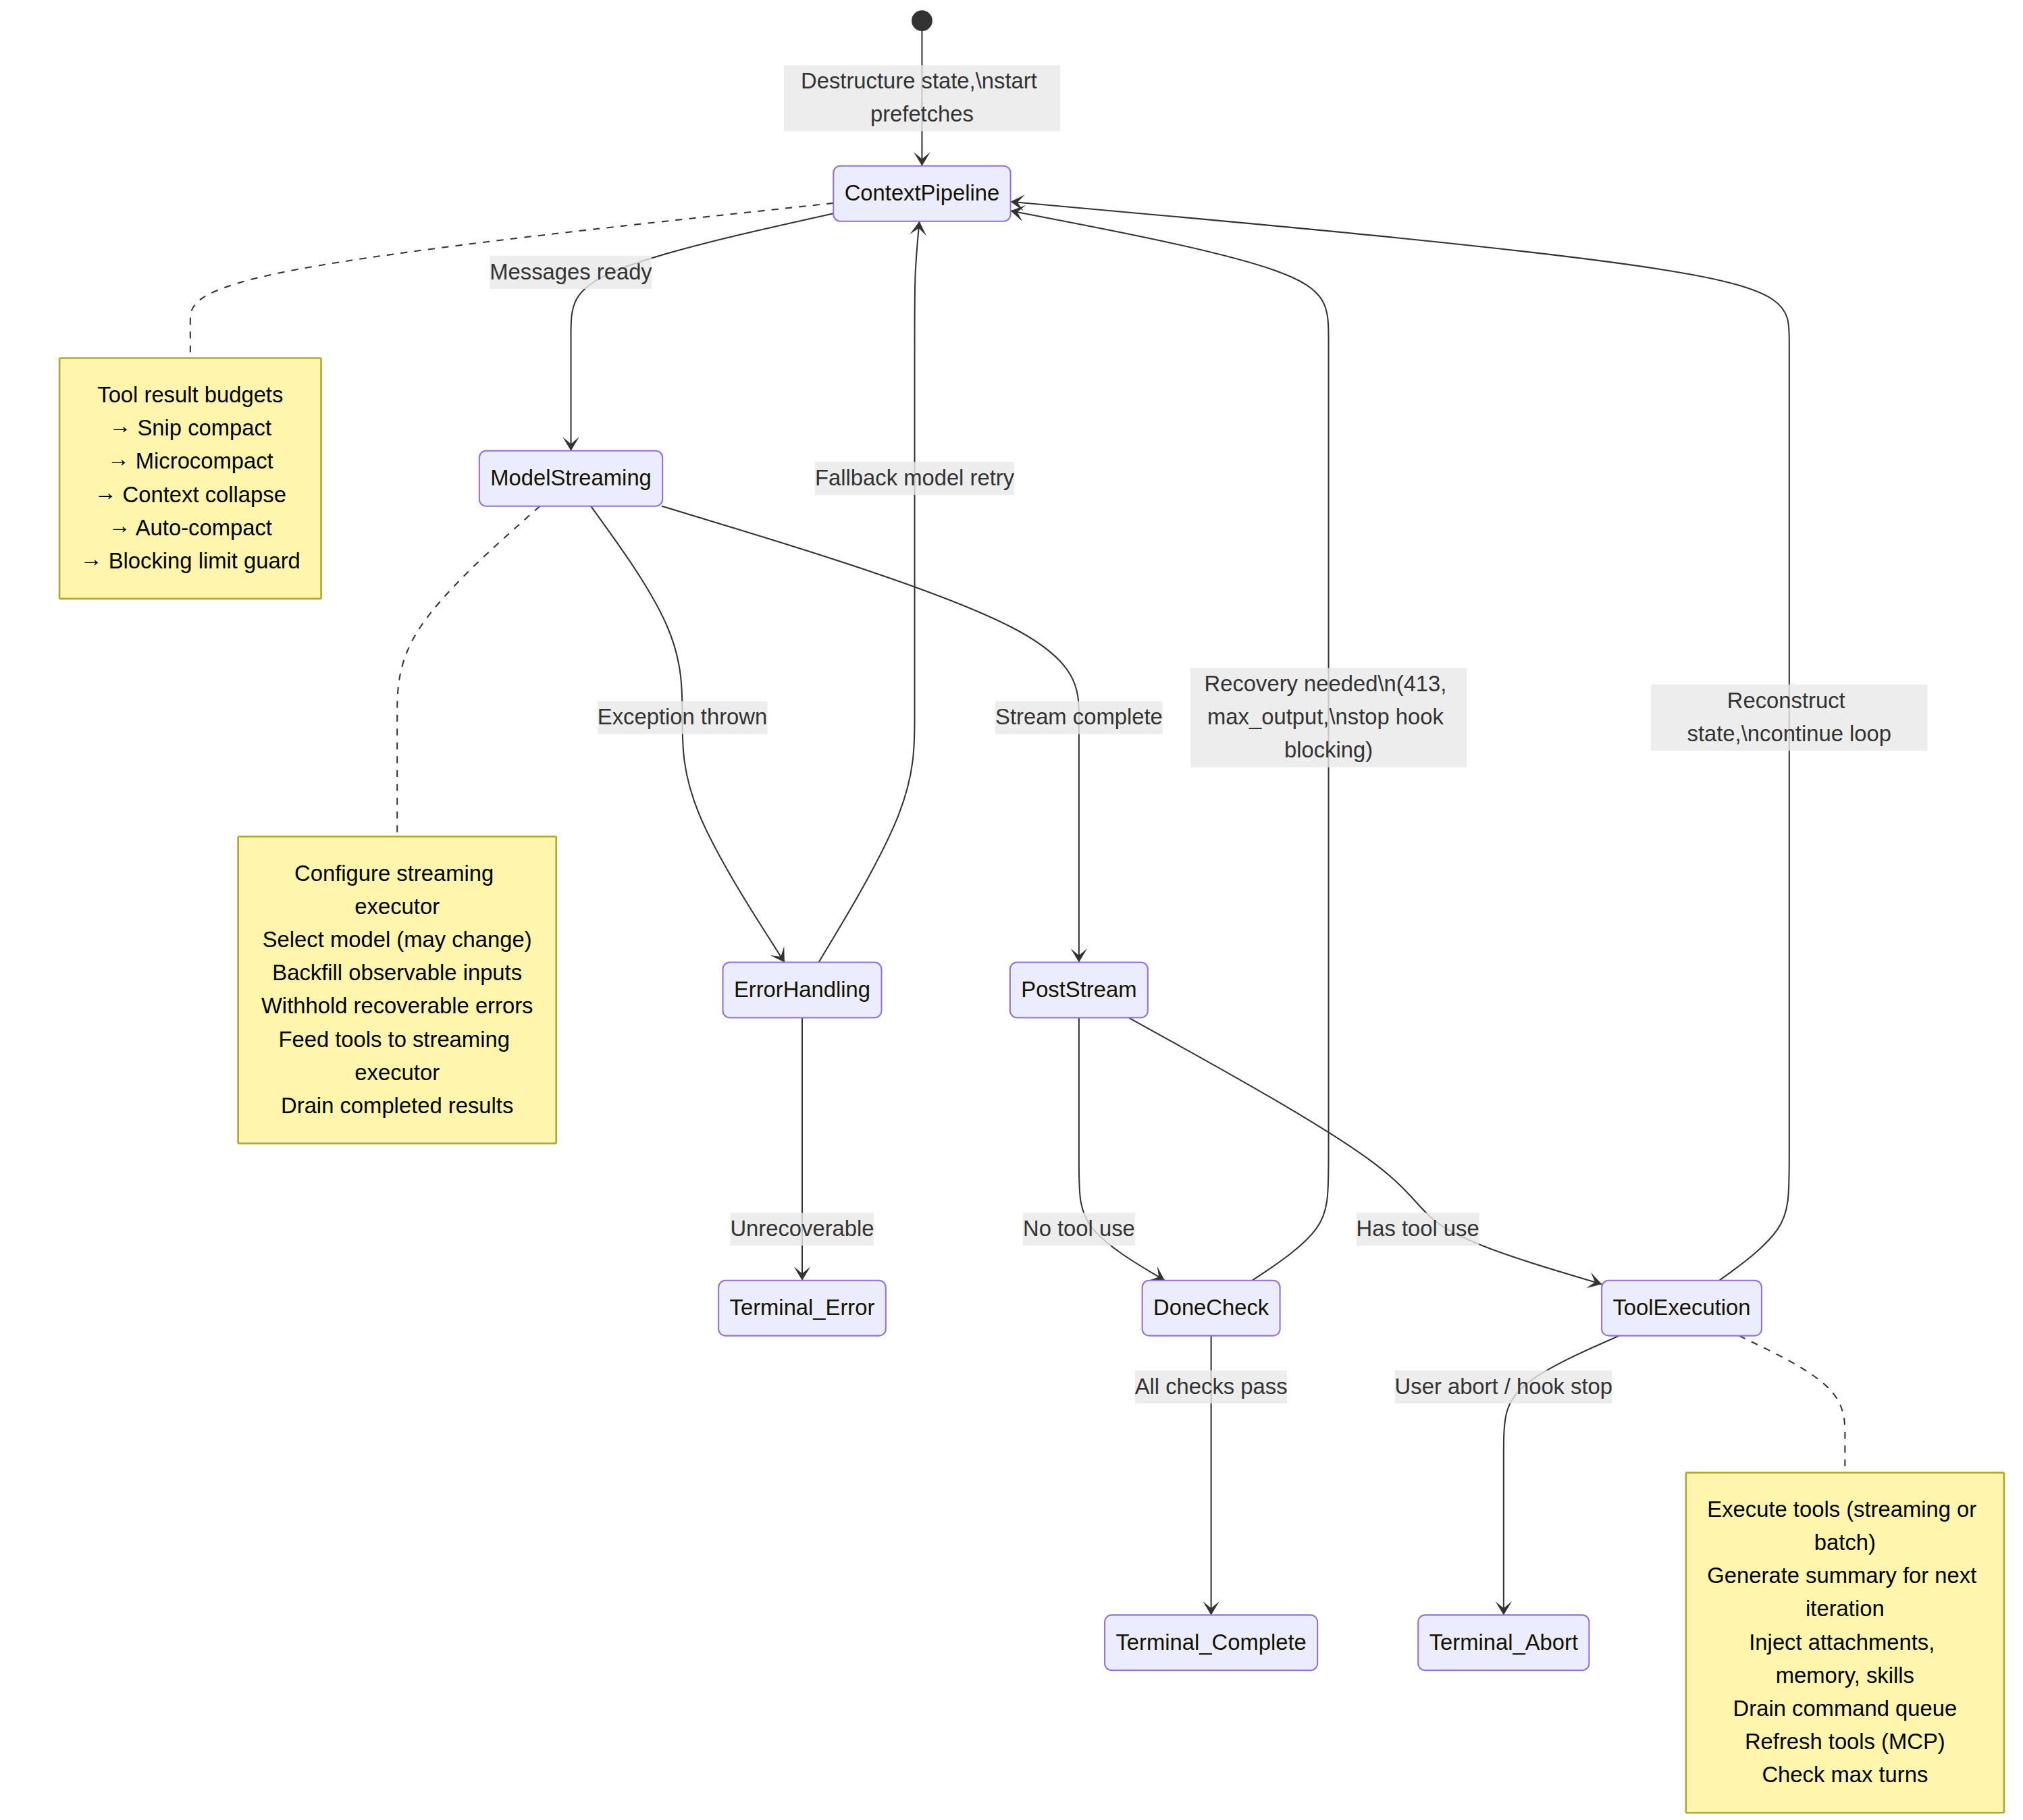
\includegraphics[width=15.54in,height=14in]{book/ch05-agent-loop_files/figure-latex/mermaid-figure-1.png}

That is the entire loop. Every feature in Claude Code -- from memory to
sub-agents to error recovery -- feeds into or consumes from this single
iteration structure.

\begin{center}\rule{0.5\linewidth}{0.5pt}\end{center}

\section{Context Management: Four Compression
Layers}\label{context-management-four-compression-layers}

Before each API call, the message history passes through up to four
context management stages. They run in a specific order, and that order
matters.

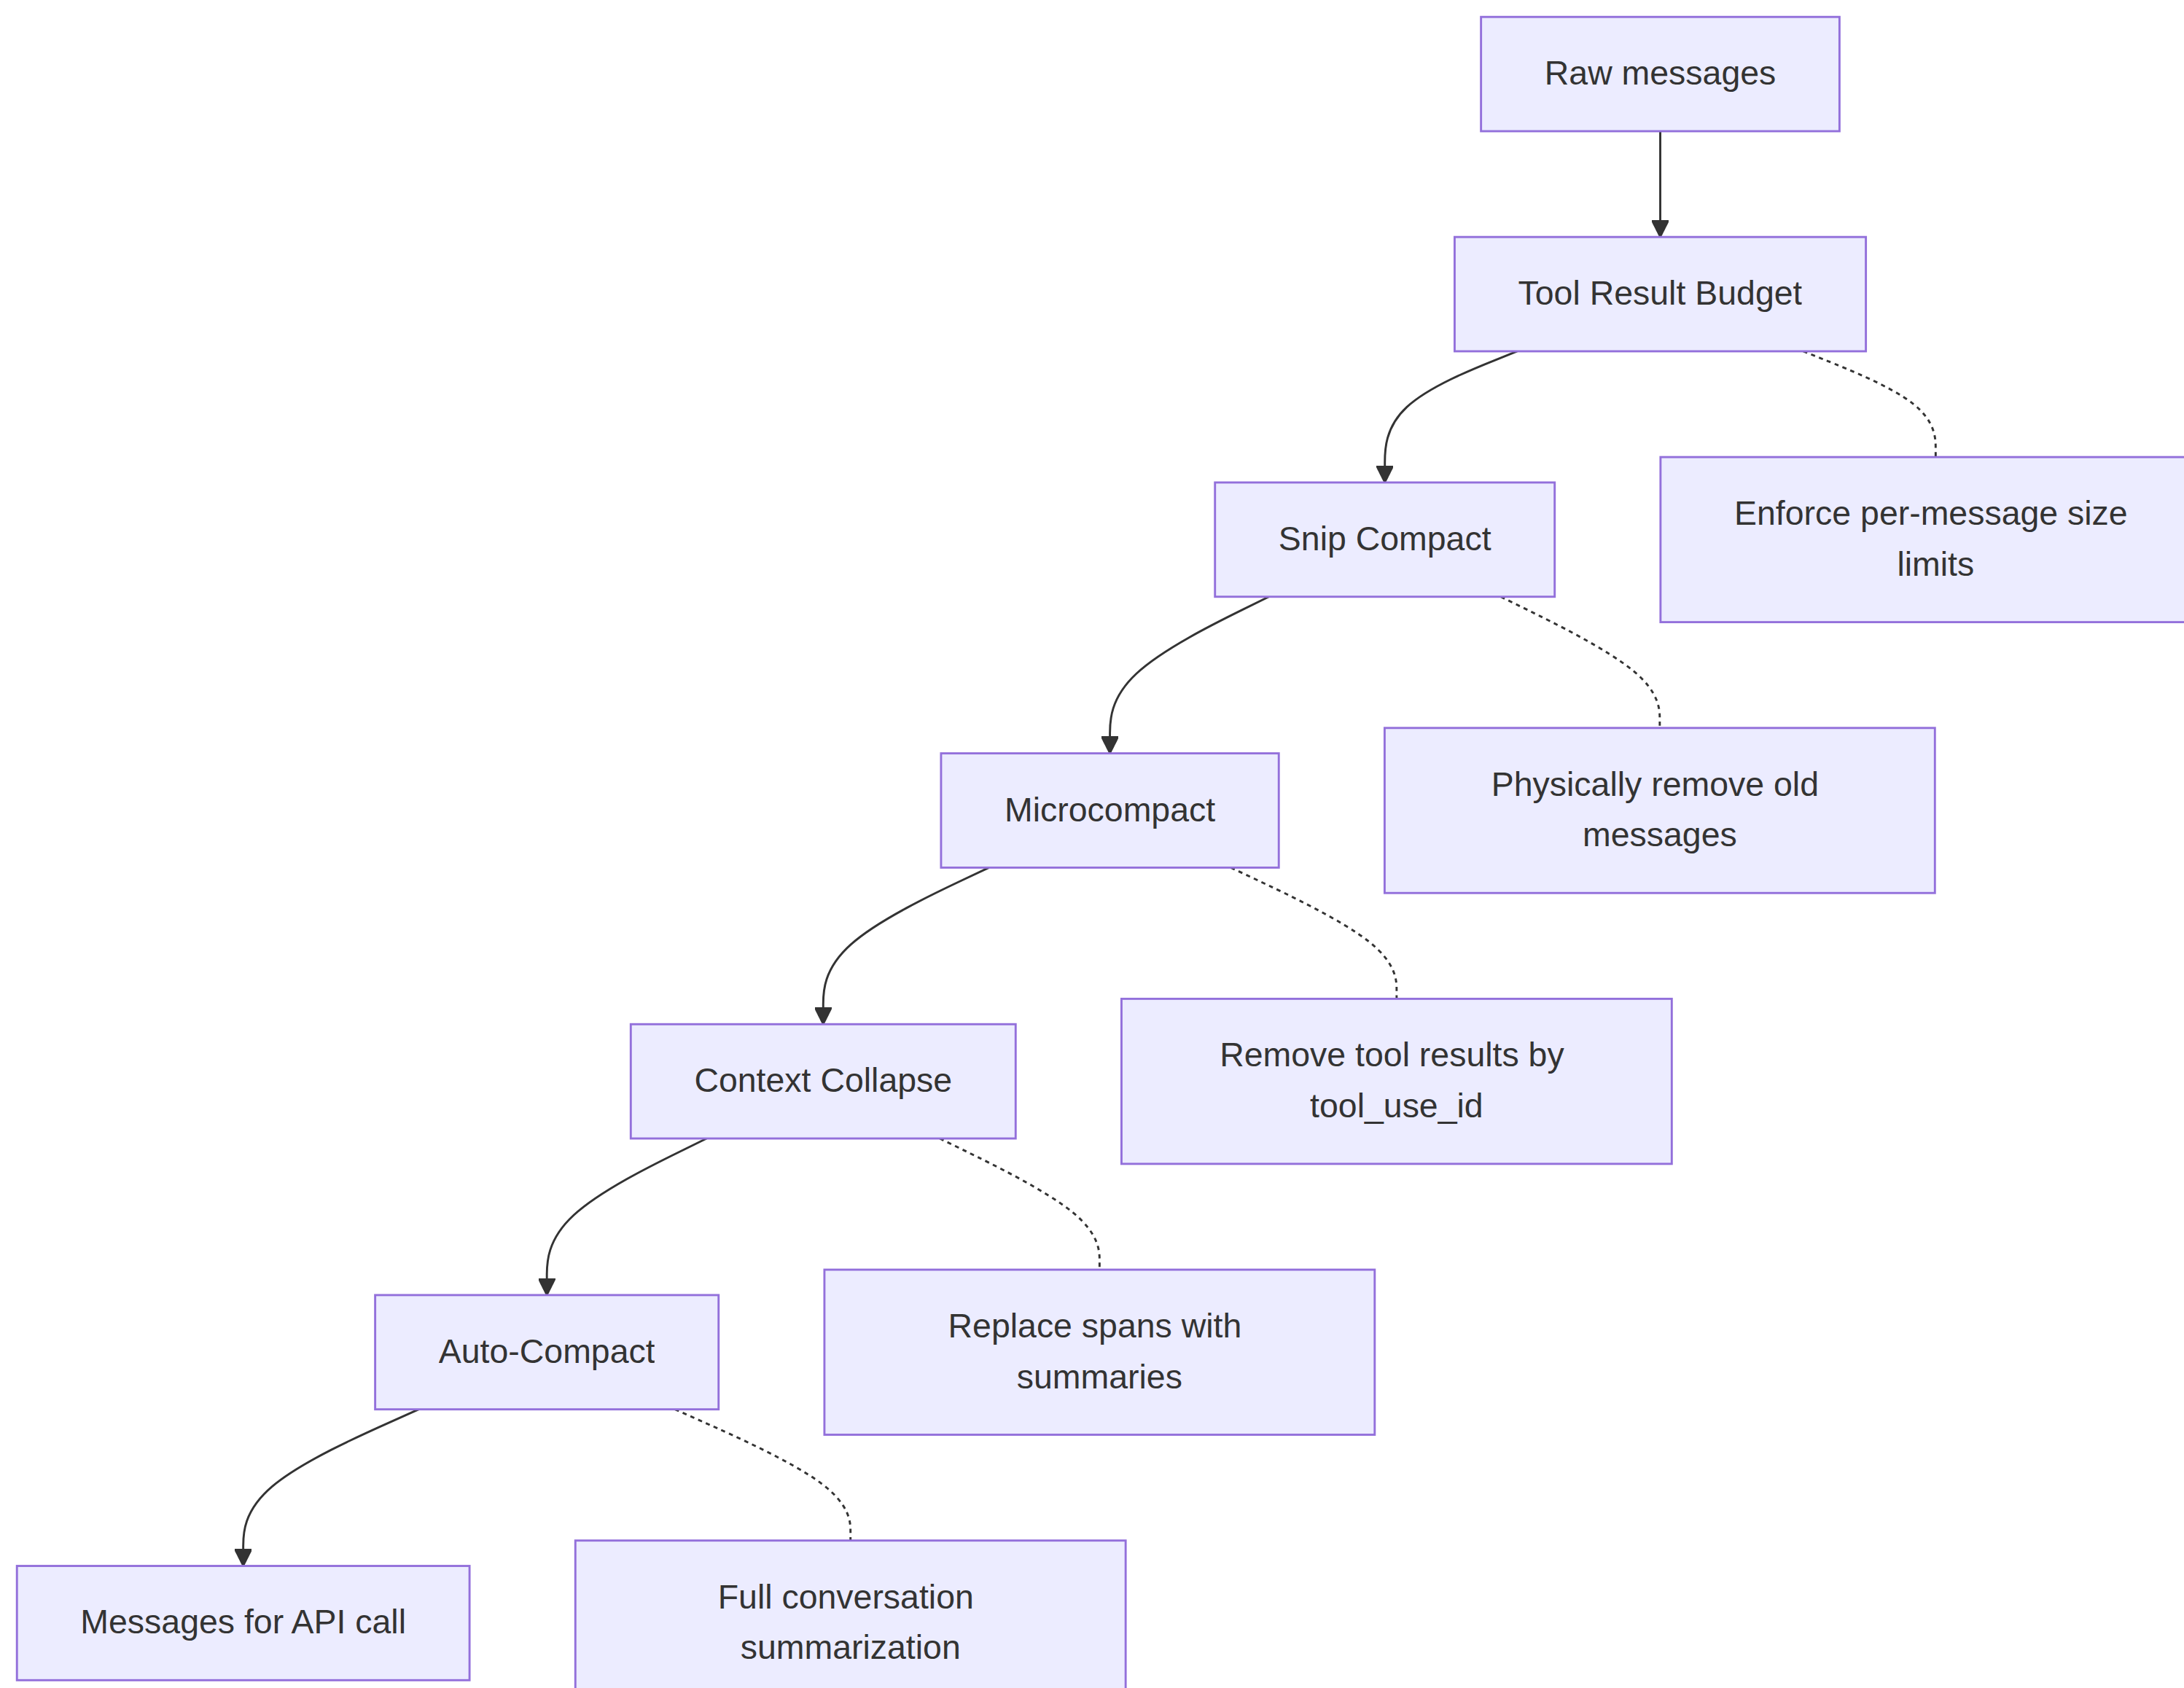
\includegraphics[width=10.96in,height=8.48in]{book/ch05-agent-loop_files/figure-latex/mermaid-figure-3.png}

\subsection{Layer 0: Tool Result
Budget}\label{layer-0-tool-result-budget}

Before any compression, \texttt{applyToolResultBudget()} enforces
per-message size limits on tool results. Tools without a finite
\texttt{maxResultSizeChars} are exempted.

\subsection{Layer 1: Snip Compact}\label{layer-1-snip-compact}

The lightest operation. Snip physically removes old messages from the
array, yielding a boundary message to signal the removal to the UI. It
reports how many tokens were freed, and that number is plumbed into
auto-compact's threshold check.

\subsection{Layer 2: Microcompact}\label{layer-2-microcompact}

Microcompact removes tool results that are no longer needed, identified
by \texttt{tool\_use\_id}. For cached microcompact (which edits the API
cache), the boundary message is deferred until after the API response.
The reason: client-side token estimates are unreliable. The actual
\texttt{cache\_deleted\_input\_tokens} from the API response tells you
what was really freed.

\subsection{Layer 3: Context Collapse}\label{layer-3-context-collapse}

Context collapse replaces spans of conversation with summaries. It runs
before auto-compact, and the ordering is deliberate: if collapse reduces
the context below the auto-compact threshold, auto-compact becomes a
no-op. This preserves granular context instead of replacing everything
with a single monolithic summary.

\subsection{Layer 4: Auto-Compact}\label{layer-4-auto-compact}

The heaviest operation: it forks an entire Claude conversation to
summarize the history. The implementation has a circuit breaker -- after
3 consecutive failures, it stops trying. This prevents the nightmare
scenario observed in production: sessions stuck over the context limit
burning 250K API calls per day in an infinite compact-fail-retry loop.

\subsection{Auto-Compact Thresholds}\label{auto-compact-thresholds}

The thresholds are derived from the model's context window:

\begin{verbatim}
effectiveContextWindow = contextWindow - min(modelMaxOutput, 20000)

Thresholds (relative to effectiveContextWindow):
  Auto-compact fires:      effectiveWindow - 13,000
  Blocking limit (hard):   effectiveWindow - 3,000
\end{verbatim}

\begin{longtable}[]{@{}
  >{\raggedright\arraybackslash}p{(\linewidth - 4\tabcolsep) * \real{0.3846}}
  >{\raggedright\arraybackslash}p{(\linewidth - 4\tabcolsep) * \real{0.2692}}
  >{\raggedright\arraybackslash}p{(\linewidth - 4\tabcolsep) * \real{0.3462}}@{}}
\toprule\noalign{}
\begin{minipage}[b]{\linewidth}\raggedright
Constant
\end{minipage} & \begin{minipage}[b]{\linewidth}\raggedright
Value
\end{minipage} & \begin{minipage}[b]{\linewidth}\raggedright
Purpose
\end{minipage} \\
\midrule\noalign{}
\endhead
\bottomrule\noalign{}
\endlastfoot
\texttt{AUTOCOMPACT\_BUFFER\_TOKENS} & 13,000 & Headroom below effective
window for auto-compact trigger \\
\texttt{MANUAL\_COMPACT\_BUFFER\_TOKENS} & 3,000 & Reserves space so
\texttt{/compact} still works \\
\texttt{MAX\_CONSECUTIVE\_AUTOCOMPACT\_FAILURES} & 3 & Circuit breaker
threshold \\
\end{longtable}

The 13,000-token buffer means auto-compact fires well before the hard
limit. The gap between the auto-compact threshold and the blocking limit
is where reactive compact operates -- if the proactive auto-compact
fails or is disabled, reactive compact catches the 413 error and
compacts on demand.

\subsection{Token Counting}\label{token-counting}

The canonical function \texttt{tokenCountWithEstimation} combines
authoritative API-reported token counts (from the most recent response)
with a rough estimate for messages added after that response. The
approximation is conservative -- it errs toward higher counts, which
means auto-compact fires slightly early rather than slightly late.

\begin{center}\rule{0.5\linewidth}{0.5pt}\end{center}

\section{Model Streaming}\label{model-streaming}

\subsection{The callModel() Loop}\label{the-callmodel-loop}

The API call happens inside a \texttt{while(attemptWithFallback)} loop
that enables model fallback:

\begin{Shaded}
\begin{Highlighting}[]
\KeywordTok{let}\NormalTok{ attemptWithFallback }\OperatorTok{=} \KeywordTok{true}
\ControlFlowTok{while}\NormalTok{ (attemptWithFallback) \{}
\NormalTok{  attemptWithFallback }\OperatorTok{=} \KeywordTok{false}
  \ControlFlowTok{try}\NormalTok{ \{}
    \ControlFlowTok{for} \ControlFlowTok{await}\NormalTok{ (}\KeywordTok{const}\NormalTok{ message }\KeywordTok{of}\NormalTok{ deps}\OperatorTok{.}\FunctionTok{callModel}\NormalTok{(\{ messages}\OperatorTok{,}\NormalTok{ systemPrompt}\OperatorTok{,}\NormalTok{ tools}\OperatorTok{,}\NormalTok{ signal \})) \{}
      \CommentTok{// Process each streamed message}
\NormalTok{    \}}
\NormalTok{  \} }\ControlFlowTok{catch}\NormalTok{ (innerError) \{}
    \ControlFlowTok{if}\NormalTok{ (innerError }\KeywordTok{instanceof}\NormalTok{ FallbackTriggeredError }\OperatorTok{\&\&}\NormalTok{ fallbackModel) \{}
\NormalTok{      currentModel }\OperatorTok{=}\NormalTok{ fallbackModel}
\NormalTok{      attemptWithFallback }\OperatorTok{=} \KeywordTok{true}
      \ControlFlowTok{continue}
\NormalTok{    \}}
    \ControlFlowTok{throw}\NormalTok{ innerError}
\NormalTok{  \}}
\NormalTok{\}}
\end{Highlighting}
\end{Shaded}

When enabled, a \texttt{StreamingToolExecutor} starts executing tools as
soon as their \texttt{tool\_use} blocks arrive during streaming -- not
after the full response completes. How tools are orchestrated into
concurrent batches is the subject of Chapter 7.

\subsection{The Withholding Pattern}\label{the-withholding-pattern}

This is one of the most important patterns in the file. Recoverable
errors are suppressed from the yield stream:

\begin{Shaded}
\begin{Highlighting}[]
\KeywordTok{let}\NormalTok{ withheld }\OperatorTok{=} \KeywordTok{false}
\ControlFlowTok{if}\NormalTok{ (contextCollapse}\OperatorTok{?.}\FunctionTok{isWithheldPromptTooLong}\NormalTok{(message)) withheld }\OperatorTok{=} \KeywordTok{true}
\ControlFlowTok{if}\NormalTok{ (reactiveCompact}\OperatorTok{?.}\FunctionTok{isWithheldPromptTooLong}\NormalTok{(message)) withheld }\OperatorTok{=} \KeywordTok{true}
\ControlFlowTok{if}\NormalTok{ (}\FunctionTok{isWithheldMaxOutputTokens}\NormalTok{(message)) withheld }\OperatorTok{=} \KeywordTok{true}
\ControlFlowTok{if}\NormalTok{ (}\OperatorTok{!}\NormalTok{withheld) }\KeywordTok{yield}\NormalTok{ yieldMessage}
\end{Highlighting}
\end{Shaded}

Why withhold? Because SDK consumers -- Cowork, the desktop app --
terminate the session on any message with an \texttt{error} field. If
you yield a prompt-too-long error and then successfully recover via
reactive compaction, the consumer has already disconnected. The recovery
loop keeps running, but nobody is listening. So the error is withheld,
pushed to \texttt{assistantMessages} so downstream recovery checks can
find it. If all recovery paths fail, the withheld message is finally
surfaced.

\subsection{Model Fallback}\label{model-fallback}

When a \texttt{FallbackTriggeredError} is caught (high demand on the
primary model), the loop switches models and retries. But thinking
signatures are model-bound -- replaying a protected-thinking block from
one model to a different fallback model causes a 400 error. The code
strips signature blocks before retry. All orphaned assistant messages
from the failed attempt are tombstoned so the UI removes them.

\begin{center}\rule{0.5\linewidth}{0.5pt}\end{center}

\section{Error Recovery: The Escalation
Ladder}\label{error-recovery-the-escalation-ladder}

Error recovery in query.ts is not a single strategy. It is a ladder of
increasingly aggressive interventions, each triggered when the previous
one fails.

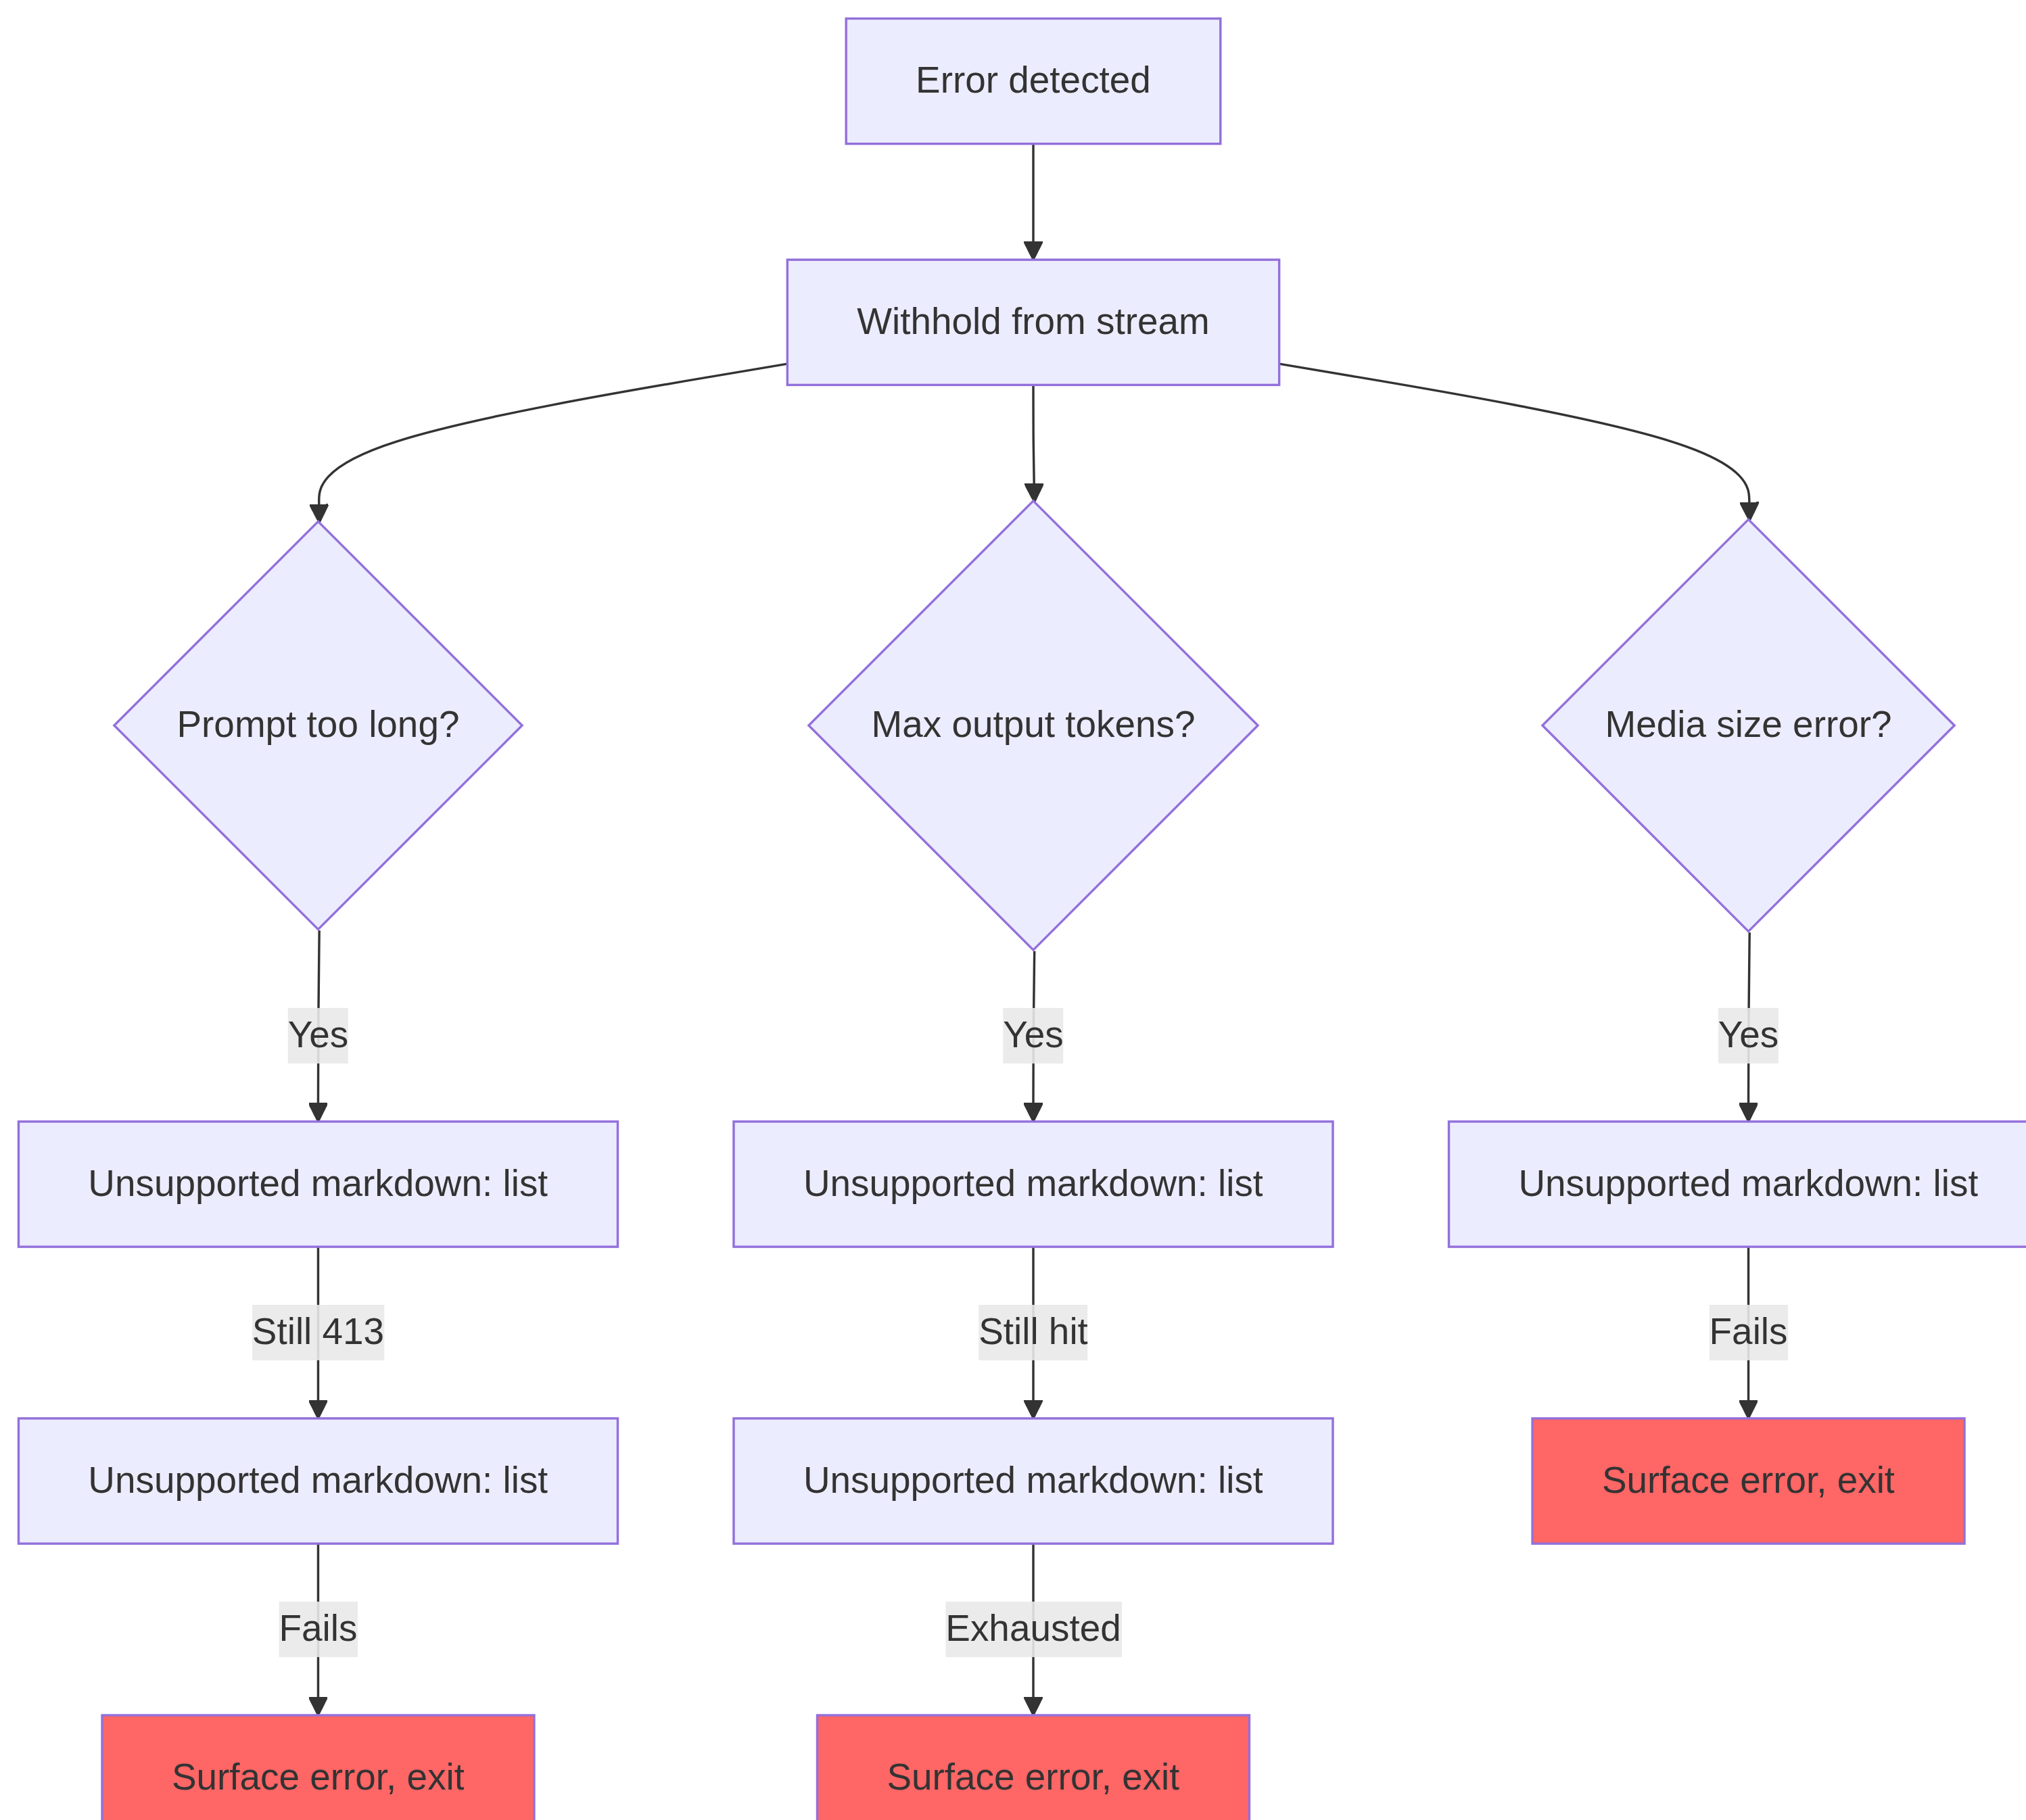
\includegraphics[width=9.28in,height=8.35in]{book/ch05-agent-loop_files/figure-latex/mermaid-figure-2.png}

\subsection{The Death Spiral Guard}\label{the-death-spiral-guard}

The most dangerous failure mode is an infinite loop. The code has
multiple guards:

\begin{enumerate}
\def\labelenumi{\arabic{enumi}.}
\tightlist
\item
  \textbf{\texttt{hasAttemptedReactiveCompact}}: One-shot flag. Reactive
  compact fires once per error type.
\item
  \textbf{\texttt{MAX\_OUTPUT\_TOKENS\_RECOVERY\_LIMIT\ =\ 3}}: Hard cap
  on multi-turn recovery attempts.
\item
  \textbf{Circuit breaker on auto-compact}: After 3 consecutive
  failures, auto-compact stops trying entirely.
\item
  \textbf{No stop hooks on error responses}: The code explicitly returns
  before reaching stop hooks when the last message is an API error. The
  comment explains: ``error -\textgreater{} hook blocking
  -\textgreater{} retry -\textgreater{} error -\textgreater{} \ldots{}
  (the hook injects more tokens each cycle).''
\item
  \textbf{Preserved \texttt{hasAttemptedReactiveCompact} across stop
  hook retries}: When a stop hook returns blocking errors and forces a
  retry, the reactive compact guard is preserved. The comment documents
  the bug: ``Resetting to false here caused an infinite loop burning
  thousands of API calls.''
\end{enumerate}

Each of these guards was added because someone hit the failure mode in
production.

\begin{center}\rule{0.5\linewidth}{0.5pt}\end{center}

\section{Worked Example: ``Fix the Bug in
auth.ts''}\label{worked-example-fix-the-bug-in-auth.ts}

To make the loop concrete, let us trace a real interaction through three
iterations.

\textbf{The user types:}
\texttt{Fix\ the\ null\ pointer\ bug\ in\ src/auth/validate.ts}

\textbf{Iteration 1: The model reads the file.}

The loop enters. Context management runs (no compression needed -- the
conversation is short). The model streams a response: ``Let me look at
the file.'' It emits a single \texttt{tool\_use} block:
\texttt{Read(\{\ file\_path:\ "src/auth/validate.ts"\ \})}. The
streaming executor sees a concurrency-safe tool and starts it
immediately. By the time the model finishes its response text, the file
contents are already in memory.

Post-stream processing: the model used a tool, so we enter the tool-use
path. The Read result (file contents with line numbers) is pushed to
\texttt{toolResults}. A Haiku summary promise is kicked off in the
background. State is reconstructed with the new messages,
\texttt{transition:\ \{\ reason:\ \textquotesingle{}next\_turn\textquotesingle{}\ \}},
and the loop continues.

\textbf{Iteration 2: The model edits the file.}

Context management runs again (still under the threshold). The model
streams: ``I see the bug on line 42 -- \texttt{userId} can be null.'' It
emits
\texttt{Edit(\{\ file\_path:\ "src/auth/validate.ts",\ old\_string:\ "const\ user\ =\ getUser(userId)",\ new\_string:\ "if\ (!userId)\ return\ \{\ error:\ \textquotesingle{}unauthorized\textquotesingle{}\ \}\textbackslash{}nconst\ user\ =\ getUser(userId)"\ \})}.

Edit is not concurrency-safe, so the streaming executor queues it until
the response completes. Then the 14-step execution pipeline fires: Zod
validation passes, input backfill expands the path, the PreToolUse hook
checks permissions (the user approves), and the edit is applied. The
pending Haiku summary from iteration 1 resolves during streaming -- its
result is yielded as a \texttt{ToolUseSummaryMessage}. State is
reconstructed, loop continues.

\textbf{Iteration 3: The model declares completion.}

The model streams: ``I've fixed the null pointer bug by adding a guard
clause.'' No \texttt{tool\_use} blocks. We enter the ``done'' path.
Prompt-too-long recovery? Not needed. Max output tokens? No.~Stop hooks
run -- no blocking errors. Token budget check passes. The loop returns
\texttt{\{\ reason:\ \textquotesingle{}completed\textquotesingle{}\ \}}.

Total: three API calls, two tool executions, one user permission prompt.
The loop handled streaming tool execution, Haiku summarization
overlapping with the API call, and the full permission pipeline -- all
through the same \texttt{while(true)} structure.

\begin{center}\rule{0.5\linewidth}{0.5pt}\end{center}

\section{Token Budgets}\label{token-budgets}

Users can request a token budget for a turn (e.g., \texttt{+500k}). The
budget system decides whether to continue or stop after the model
completes a response.

\texttt{checkTokenBudget} makes a binary continue/stop decision with
three rules:

\begin{enumerate}
\def\labelenumi{\arabic{enumi}.}
\tightlist
\item
  \textbf{Subagents always stop.} Budget is a top-level concept only.
\item
  \textbf{Completion threshold at 90\%.} If
  \texttt{turnTokens\ \textless{}\ budget\ *\ 0.9}, continue.
\item
  \textbf{Diminishing returns detection.} After 3+ continuations, if
  both the current and previous delta are below 500 tokens, stop early.
  The model is producing less and less output per continuation.
\end{enumerate}

When the decision is ``continue,'' a nudge message is injected telling
the model how much budget remains.

\begin{center}\rule{0.5\linewidth}{0.5pt}\end{center}

\section{Stop Hooks: Forcing the Model to Keep
Working}\label{stop-hooks-forcing-the-model-to-keep-working}

Stop hooks run when the model finishes without requesting any tool use
-- it thinks it is done. The hooks evaluate whether it actually
\emph{is} done.

The pipeline runs template job classification, fires background tasks
(prompt suggestion, memory extraction), and then executes stop hooks
proper. When a stop hook returns blocking errors -- ``you said you were
done, but the linter found 3 errors'' -- the errors are appended to the
message history and the loop continues with
\texttt{stopHookActive:\ true}. This flag prevents re-running the same
hooks on the retry.

When a stop hook signals \texttt{preventContinuation}, the loop exits
immediately with
\texttt{\{\ reason:\ \textquotesingle{}stop\_hook\_prevented\textquotesingle{}\ \}}.

\begin{center}\rule{0.5\linewidth}{0.5pt}\end{center}

\section{State Transitions: The Complete
Catalog}\label{state-transitions-the-complete-catalog}

Every exit from the loop is one of two types: a \texttt{Terminal} (the
loop returns) or a \texttt{Continue} (the loop iterates).

\subsection{Terminal States (10
reasons)}\label{terminal-states-10-reasons}

\begin{longtable}[]{@{}
  >{\raggedright\arraybackslash}p{(\linewidth - 2\tabcolsep) * \real{0.4706}}
  >{\raggedright\arraybackslash}p{(\linewidth - 2\tabcolsep) * \real{0.5294}}@{}}
\toprule\noalign{}
\begin{minipage}[b]{\linewidth}\raggedright
Reason
\end{minipage} & \begin{minipage}[b]{\linewidth}\raggedright
Trigger
\end{minipage} \\
\midrule\noalign{}
\endhead
\bottomrule\noalign{}
\endlastfoot
\texttt{blocking\_limit} & Token count at hard limit, auto-compact
OFF \\
\texttt{image\_error} & ImageSizeError, ImageResizeError, or
unrecoverable media error \\
\texttt{model\_error} & Unrecoverable API/model exception \\
\texttt{aborted\_streaming} & User abort during model streaming \\
\texttt{prompt\_too\_long} & Withheld 413 after all recovery
exhausted \\
\texttt{completed} & Normal completion (no tool use, or budget
exhausted, or API error) \\
\texttt{stop\_hook\_prevented} & Stop hook explicitly blocked
continuation \\
\texttt{aborted\_tools} & User abort during tool execution \\
\texttt{hook\_stopped} & PreToolUse hook stopped continuation \\
\texttt{max\_turns} & Hit the \texttt{maxTurns} limit \\
\end{longtable}

\subsection{Continue States (7
reasons)}\label{continue-states-7-reasons}

\begin{longtable}[]{@{}
  >{\raggedright\arraybackslash}p{(\linewidth - 2\tabcolsep) * \real{0.4706}}
  >{\raggedright\arraybackslash}p{(\linewidth - 2\tabcolsep) * \real{0.5294}}@{}}
\toprule\noalign{}
\begin{minipage}[b]{\linewidth}\raggedright
Reason
\end{minipage} & \begin{minipage}[b]{\linewidth}\raggedright
Trigger
\end{minipage} \\
\midrule\noalign{}
\endhead
\bottomrule\noalign{}
\endlastfoot
\texttt{collapse\_drain\_retry} & Context collapse drained staged
collapses on 413 \\
\texttt{reactive\_compact\_retry} & Reactive compact succeeded after 413
or media error \\
\texttt{max\_output\_tokens\_escalate} & 8K cap hit, escalating to
64K \\
\texttt{max\_output\_tokens\_recovery} & 64K still hit, multi-turn
recovery (up to 3 attempts) \\
\texttt{stop\_hook\_blocking} & Stop hook returned blocking errors, must
retry \\
\texttt{token\_budget\_continuation} & Token budget not exhausted, nudge
message injected \\
\texttt{next\_turn} & Normal tool-use continuation \\
\end{longtable}

\begin{center}\rule{0.5\linewidth}{0.5pt}\end{center}

\section{Orphaned Tool Results: The Protocol Safety
Net}\label{orphaned-tool-results-the-protocol-safety-net}

The API protocol requires that every \texttt{tool\_use} block is
followed by a \texttt{tool\_result}. The function
\texttt{yieldMissingToolResultBlocks} creates error
\texttt{tool\_result} messages for every \texttt{tool\_use} block that
the model emitted but that never got a corresponding result. Without
this safety net, a crash during streaming would leave orphaned
\texttt{tool\_use} blocks that would cause a protocol error on the next
API call.

It fires in three places: the outer error handler (model crash), the
fallback handler (model switch mid-stream), and the abort handler (user
interruption). Each path has a different error message, but the
mechanism is identical.

\begin{center}\rule{0.5\linewidth}{0.5pt}\end{center}

\section{Abort Handling: Two Paths}\label{abort-handling-two-paths}

Aborts can happen at two points: during streaming and during tool
execution. Each has distinct behavior.

\textbf{Abort during streaming}: The streaming executor (if active)
drains remaining results, generating synthetic \texttt{tool\_results}
for queued tools. Without the executor,
\texttt{yieldMissingToolResultBlocks} fills the gap. The
\texttt{signal.reason} check distinguishes between a hard abort (Ctrl+C)
and a submit-interrupt (user typed a new message) -- submit-interrupts
skip the interruption message because the queued user message already
provides context.

\textbf{Abort during tool execution}: Similar logic, with a
\texttt{toolUse:\ true} parameter on the interruption message signaling
to the UI that tools were in progress.

\begin{center}\rule{0.5\linewidth}{0.5pt}\end{center}

\section{The Thinking Rules}\label{the-thinking-rules}

Claude's thinking/redacted\_thinking blocks have three inviolable rules:

\begin{enumerate}
\def\labelenumi{\arabic{enumi}.}
\tightlist
\item
  A message containing a thinking block must be part of a query whose
  \texttt{max\_thinking\_length\ \textgreater{}\ 0}
\item
  A thinking block may not be the last block in a message
\item
  Thinking blocks must be preserved for the duration of an assistant
  trajectory
\end{enumerate}

Violating any of these produces opaque API errors. The code handles them
in several places: the fallback handler strips signature blocks (which
are model-bound), the compaction pipeline preserves the protected tail,
and the microcompact layer never touches thinking blocks.

\begin{center}\rule{0.5\linewidth}{0.5pt}\end{center}

\section{Dependency Injection}\label{dependency-injection}

The \texttt{QueryDeps} type is intentionally narrow -- four
dependencies, not forty:

Four injected dependencies: the model caller, the compactor, the
microcompactor, and a UUID generator. Tests pass \texttt{deps} into the
loop params to inject fakes directly. Using \texttt{typeof\ fn} for the
type definitions keeps the signatures in sync automatically. Alongside
the mutable \texttt{State} and the injectable \texttt{QueryDeps}, an
immutable \texttt{QueryConfig} is snapshotted once at \texttt{query()}
entry -- feature flags, session state, and environment variables
captured once and never re-read. The three-way separation (mutable
state, immutable config, injectable deps) makes the loop testable and
makes the eventual refactor to a pure
\texttt{step(state,\ event,\ config)} reducer straightforward.

\begin{center}\rule{0.5\linewidth}{0.5pt}\end{center}

\section{Apply This: Building Your Own Agent
Loop}\label{apply-this-building-your-own-agent-loop}

\textbf{Use a generator, not callbacks.} The backpressure is free. The
return value semantics are free. The composability via \texttt{yield*}
is free. Agent loops are strictly forward-moving -- you never need to
rewind or fork.

\textbf{Make state transitions explicit.} Reconstruct the full state
object at every \texttt{continue} site. The verbosity is the feature --
it prevents partial-update bugs and makes each transition
self-documenting.

\textbf{Withhold recoverable errors.} If your consumers disconnect on
errors, do not yield errors until you know recovery has failed. Push
them to an internal buffer, attempt recovery, and surface only on
exhaustion.

\textbf{Layer your context management.} Light operations first
(removal), heavy operations last (summarization). This preserves
granular context when possible and falls back to monolithic summaries
only when necessary.

\textbf{Add circuit breakers for every retry.} Every recovery mechanism
in \texttt{query.ts} has an explicit limit: 3 auto-compact failures, 3
max-output recovery attempts, 1 reactive compact attempt. Without these
limits, the first production session that triggers a retry-on-failure
loop will burn your API budget overnight.

The minimal agent loop skeleton, if you are starting from scratch:

\begin{verbatim}
async function* agentLoop(params) {
  let state = initState(params)
  while (true) {
    const context = compressIfNeeded(state.messages)
    const response = await callModel(context)
    if (response.error) {
      if (canRecover(response.error, state)) { state = recoverState(state); continue }
      return { reason: 'error' }
    }
    if (!response.toolCalls.length) return { reason: 'completed' }
    const results = await executeTools(response.toolCalls)
    state = { ...state, messages: [...context, response.message, ...results] }
  }
}
\end{verbatim}

Every feature in Claude Code's loop is an elaboration of one of these
steps. The four compression layers elaborate step 3 (compress). The
withholding pattern elaborates the model call. The escalation ladder
elaborates error recovery. Stop hooks elaborate the ``no tool use''
exit. Start with this skeleton. Add each elaboration only when you hit
the problem it solves.

\begin{center}\rule{0.5\linewidth}{0.5pt}\end{center}

\section{Summary}\label{summary}

The agent loop is 1,730 lines of a single \texttt{while(true)} that does
everything. It streams model responses, executes tools concurrently,
compresses context through four layers, recovers from five categories of
errors, tracks token budgets with diminishing returns detection, runs
stop hooks that can force the model back to work, manages prefetch
pipelines for memory and skills, and produces a typed discriminated
union of exactly why it stopped.

It is the most important file in the system because it is the only file
that touches every other subsystem. The context pipeline feeds into it.
The tool system feeds out of it. The error recovery wraps around it. The
hooks intercept it. The state layer persists through it. The UI renders
from it.

If you understand \texttt{query()}, you understand Claude Code.
Everything else is a peripheral.

\chapter{Chapter 6: Tools -- From Definition to
Execution}\label{chapter-6-tools-from-definition-to-execution}

\section{The Nervous System}\label{the-nervous-system}

Chapter 5 showed you the agent loop -- the \texttt{while(true)} that
streams model responses, collects tool calls, and feeds results back.
The loop is the heartbeat. But the heartbeat is meaningless without the
nervous system that translates ``the model wants to run
\texttt{git\ status}'' into an actual shell command, with permission
checks, result budgeting, and error handling.

The tool system is that nervous system. It spans 40+ tool
implementations, a centralized registry with feature-flag gating, a
14-step execution pipeline, a permission resolver with seven modes, and
a streaming executor that starts tools before the model finishes its
response.

Every tool call in Claude Code -- every file read, every shell command,
every grep, every sub-agent dispatch -- flows through the same pipeline.
The uniformity is the point: whether the tool is a built-in Bash
executor or a third-party MCP server, it gets the same validation, the
same permission checks, the same result budgeting, the same error
classification.

The \texttt{Tool} interface has approximately 45 members. That sounds
overwhelming, but only five matter for understanding how the system
works:

\begin{enumerate}
\def\labelenumi{\arabic{enumi}.}
\tightlist
\item
  \textbf{\texttt{call()}} -- execute the tool
\item
  \textbf{\texttt{inputSchema}} -- validate and parse the input
\item
  \textbf{\texttt{isConcurrencySafe()}} -- can this run in parallel?
\item
  \textbf{\texttt{checkPermissions()}} -- is this allowed?
\item
  \textbf{\texttt{validateInput()}} -- does this input make semantic
  sense?
\end{enumerate}

Everything else -- the 12 rendering methods, the analytics hooks, the
search hints -- exists to support the UI and telemetry layers. Start
with the five, and the rest falls into place.

\begin{center}\rule{0.5\linewidth}{0.5pt}\end{center}

\section{The Tool Interface}\label{the-tool-interface}

\subsection{Three Type Parameters}\label{three-type-parameters}

Every tool is parameterized over three types:

\begin{Shaded}
\begin{Highlighting}[]
\NormalTok{Tool}\OperatorTok{\textless{}}\NormalTok{Input }\KeywordTok{extends}\NormalTok{ AnyObject}\OperatorTok{,}\NormalTok{ Output}\OperatorTok{,}\NormalTok{ P }\KeywordTok{extends}\NormalTok{ ToolProgressData}\OperatorTok{\textgreater{}}
\end{Highlighting}
\end{Shaded}

\texttt{Input} is a Zod object schema that serves double duty: it
generates the JSON Schema sent to the API (so the model knows what
parameters to provide), and it validates the model's response at runtime
via \texttt{safeParse}. \texttt{Output} is the TypeScript type of the
tool's result. \texttt{P} is the progress event type the tool emits
while running -- BashTool emits stdout chunks, GrepTool emits match
counts, AgentTool emits sub-agent transcripts.

\subsection{buildTool() and Fail-Closed
Defaults}\label{buildtool-and-fail-closed-defaults}

No tool definition directly constructs a \texttt{Tool} object. Every
tool passes through \texttt{buildTool()}, a factory that spreads a
defaults object under the tool-specific definition:

\begin{Shaded}
\begin{Highlighting}[]
\CommentTok{// Pseudocode — illustrates the fail{-}closed defaults pattern}
\KeywordTok{const}\NormalTok{ SAFE\_DEFAULTS }\OperatorTok{=}\NormalTok{ \{}
\NormalTok{  isEnabled}\OperatorTok{:}\NormalTok{         () }\KeywordTok{=\textgreater{}} \KeywordTok{true}\OperatorTok{,}
\NormalTok{  isParallelSafe}\OperatorTok{:}\NormalTok{    () }\KeywordTok{=\textgreater{}} \KeywordTok{false}\OperatorTok{,}   \CommentTok{// Fail{-}closed: new tools run serially}
\NormalTok{  isReadOnly}\OperatorTok{:}\NormalTok{        () }\KeywordTok{=\textgreater{}} \KeywordTok{false}\OperatorTok{,}   \CommentTok{// Fail{-}closed: treated as writes}
\NormalTok{  isDestructive}\OperatorTok{:}\NormalTok{     () }\KeywordTok{=\textgreater{}} \KeywordTok{false}\OperatorTok{,}
\NormalTok{  checkPermissions}\OperatorTok{:}\NormalTok{  (input) }\KeywordTok{=\textgreater{}}\NormalTok{ (\{ behavior}\OperatorTok{:} \StringTok{\textquotesingle{}allow\textquotesingle{}}\OperatorTok{,}\NormalTok{ updatedInput}\OperatorTok{:}\NormalTok{ input \})}\OperatorTok{,}
\NormalTok{\}}

\KeywordTok{function} \FunctionTok{buildTool}\NormalTok{(definition) \{}
  \ControlFlowTok{return}\NormalTok{ \{ }\OperatorTok{...}\NormalTok{SAFE\_DEFAULTS}\OperatorTok{,} \OperatorTok{...}\NormalTok{definition \}  }\CommentTok{// Definition overrides defaults}
\NormalTok{\}}
\end{Highlighting}
\end{Shaded}

The defaults are deliberately fail-closed where it matters for safety. A
new tool that forgets to implement \texttt{isConcurrencySafe} defaults
to \texttt{false} -- it runs serially, never in parallel. A tool that
forgets \texttt{isReadOnly} defaults to \texttt{false} -- the system
treats it as a write operation. A tool that forgets
\texttt{toAutoClassifierInput} returns an empty string -- the auto-mode
security classifier skips it, which means the general permission system
handles it instead of an automated bypass.

The one default that is \emph{not} fail-closed is
\texttt{checkPermissions}, which returns \texttt{allow}. This seems
backwards until you understand the layered permission model:
\texttt{checkPermissions} is tool-specific logic that runs \emph{after}
the general permission system has already evaluated rules, hooks, and
mode-based policies. A tool returning \texttt{allow} from
\texttt{checkPermissions} is saying ``I have no tool-specific
objection'' -- it is not granting blanket access. The grouping into
sub-objects (\texttt{options}, named fields like \texttt{readFileState})
provides the structure that focused interfaces would provide, without
the ceremony of declaring, implementing, and threading five separate
interface types through 40+ call sites.

\subsection{Concurrency Is
Input-Dependent}\label{concurrency-is-input-dependent}

The signature
\texttt{isConcurrencySafe(input:\ z.infer\textless{}Input\textgreater{}):\ boolean}
takes the parsed input because the same tool can be safe for some inputs
and unsafe for others. BashTool is the canonical example:
\texttt{ls\ -la} is read-only and concurrency-safe, but
\texttt{rm\ -rf\ /tmp/build} is not. The tool parses the command,
classifies each subcommand against known-safe sets, and returns
\texttt{true} only when every non-neutral part is a search or read
operation.

\subsection{The ToolResult Return
Type}\label{the-toolresult-return-type}

Every \texttt{call()} returns a
\texttt{ToolResult\textless{}T\textgreater{}}:

\begin{Shaded}
\begin{Highlighting}[]
\KeywordTok{type}\NormalTok{ ToolResult}\OperatorTok{\textless{}}\NormalTok{T}\OperatorTok{\textgreater{}} \OperatorTok{=}\NormalTok{ \{}
\NormalTok{  data}\OperatorTok{:}\NormalTok{ T}
\NormalTok{  newMessages}\OperatorTok{?:}\NormalTok{ (UserMessage }\OperatorTok{|}\NormalTok{ AssistantMessage }\OperatorTok{|}\NormalTok{ AttachmentMessage }\OperatorTok{|}\NormalTok{ SystemMessage)[]}
\NormalTok{  contextModifier}\OperatorTok{?:}\NormalTok{ (context}\OperatorTok{:}\NormalTok{ ToolUseContext) }\KeywordTok{=\textgreater{}}\NormalTok{ ToolUseContext}
\NormalTok{\}}
\end{Highlighting}
\end{Shaded}

\texttt{data} is the typed output that gets serialized into the API's
\texttt{tool\_result} content block. \texttt{newMessages} lets a tool
inject additional messages into the conversation -- AgentTool uses this
to append sub-agent transcripts. \texttt{contextModifier} is a function
that mutates the \texttt{ToolUseContext} for subsequent tools -- this is
how \texttt{EnterPlanMode} switches the permission mode. Context
modifiers are only honored for non-concurrency-safe tools; if your tool
runs in parallel, its modifier is queued until the batch completes.

\begin{center}\rule{0.5\linewidth}{0.5pt}\end{center}

\section{ToolUseContext: The God
Object}\label{toolusecontext-the-god-object}

\texttt{ToolUseContext} is the massive context bag threaded through
every tool call. It has approximately 40 fields. It is, by any
reasonable definition, a god object. It exists because the alternative
is worse.

A tool like BashTool needs the abort controller, the file state cache,
the app state, the message history, the tool set, MCP connections, and
half a dozen UI callbacks. Threading these as individual parameters
would produce function signatures with 15+ arguments. The pragmatic
solution is a single context object, grouped by concern:

\textbf{Configuration} (\texttt{options} sub-object): The tool set,
model name, MCP connections, debug flags. Set once at query start,
mostly immutable.

\textbf{Execution state}: The \texttt{abortController} for cancellation,
\texttt{readFileState} for the LRU file cache, \texttt{messages} for the
full conversation history. These change during execution.

\textbf{UI callbacks}: \texttt{setToolJSX}, \texttt{addNotification},
\texttt{requestPrompt}. Only wired in interactive (REPL) contexts. SDK
and headless modes leave them undefined.

\textbf{Agent context}: \texttt{agentId}, \texttt{renderedSystemPrompt}
(frozen parent prompt for fork sub-agents -- re-rendering could diverge
due to feature flag warm-up and bust the cache).

The sub-agent variant of \texttt{ToolUseContext} is particularly
revealing. When \texttt{createSubagentContext()} builds a context for a
child agent, it makes deliberate choices about which fields to share and
which to isolate: \texttt{setAppState} becomes a no-op for async agents,
\texttt{localDenialTracking} gets a fresh object,
\texttt{contentReplacementState} is cloned from the parent. Each choice
encodes a lesson learned from a production bug.

\begin{center}\rule{0.5\linewidth}{0.5pt}\end{center}

\section{The Registry}\label{the-registry}

\subsection{getAllBaseTools(): The Single Source of
Truth}\label{getallbasetools-the-single-source-of-truth}

The function \texttt{getAllBaseTools()} returns the exhaustive list of
every tool that could exist in the current process. Always-present tools
come first, then conditionally-included tools gated by feature flags:

\begin{Shaded}
\begin{Highlighting}[]
\KeywordTok{const}\NormalTok{ SleepTool }\OperatorTok{=} \FunctionTok{feature}\NormalTok{(}\StringTok{\textquotesingle{}PROACTIVE\textquotesingle{}}\NormalTok{) }\OperatorTok{||} \FunctionTok{feature}\NormalTok{(}\StringTok{\textquotesingle{}KAIROS\textquotesingle{}}\NormalTok{)}
  \OperatorTok{?} \PreprocessorTok{require}\NormalTok{(}\StringTok{\textquotesingle{}./tools/SleepTool/SleepTool.js\textquotesingle{}}\NormalTok{)}\OperatorTok{.}\AttributeTok{SleepTool}
  \OperatorTok{:} \DataTypeTok{null}
\end{Highlighting}
\end{Shaded}

The \texttt{feature()} import from \texttt{bun:bundle} is resolved at
bundle time. When
\texttt{feature(\textquotesingle{}AGENT\_TRIGGERS\textquotesingle{})} is
statically false, the bundler eliminates the entire \texttt{require()}
call -- dead code elimination that keeps the binary small.

\subsection{assembleToolPool(): Merging Built-in and MCP
Tools}\label{assembletoolpool-merging-built-in-and-mcp-tools}

The final tool set that reaches the model comes from
\texttt{assembleToolPool()}:

\begin{enumerate}
\def\labelenumi{\arabic{enumi}.}
\tightlist
\item
  Get built-in tools (with deny-rule filtering, REPL mode hiding, and
  \texttt{isEnabled()} checks)
\item
  Filter MCP tools by deny rules
\item
  Sort each partition alphabetically by name
\item
  Concatenate built-ins (prefix) + MCP tools (suffix)
\end{enumerate}

The sort-then-concatenate approach is not aesthetic preference. The API
server places a prompt-cache breakpoint after the last built-in tool. A
flat sort across all tools would interleave MCP tools into the built-in
list, and adding or removing an MCP tool would shift built-in tool
positions, invalidating the cache.

\begin{center}\rule{0.5\linewidth}{0.5pt}\end{center}

\section{The 14-Step Execution
Pipeline}\label{the-14-step-execution-pipeline}

The function \texttt{checkPermissionsAndCallTool()} is where intent
becomes action. Every tool call passes through these 14 steps.

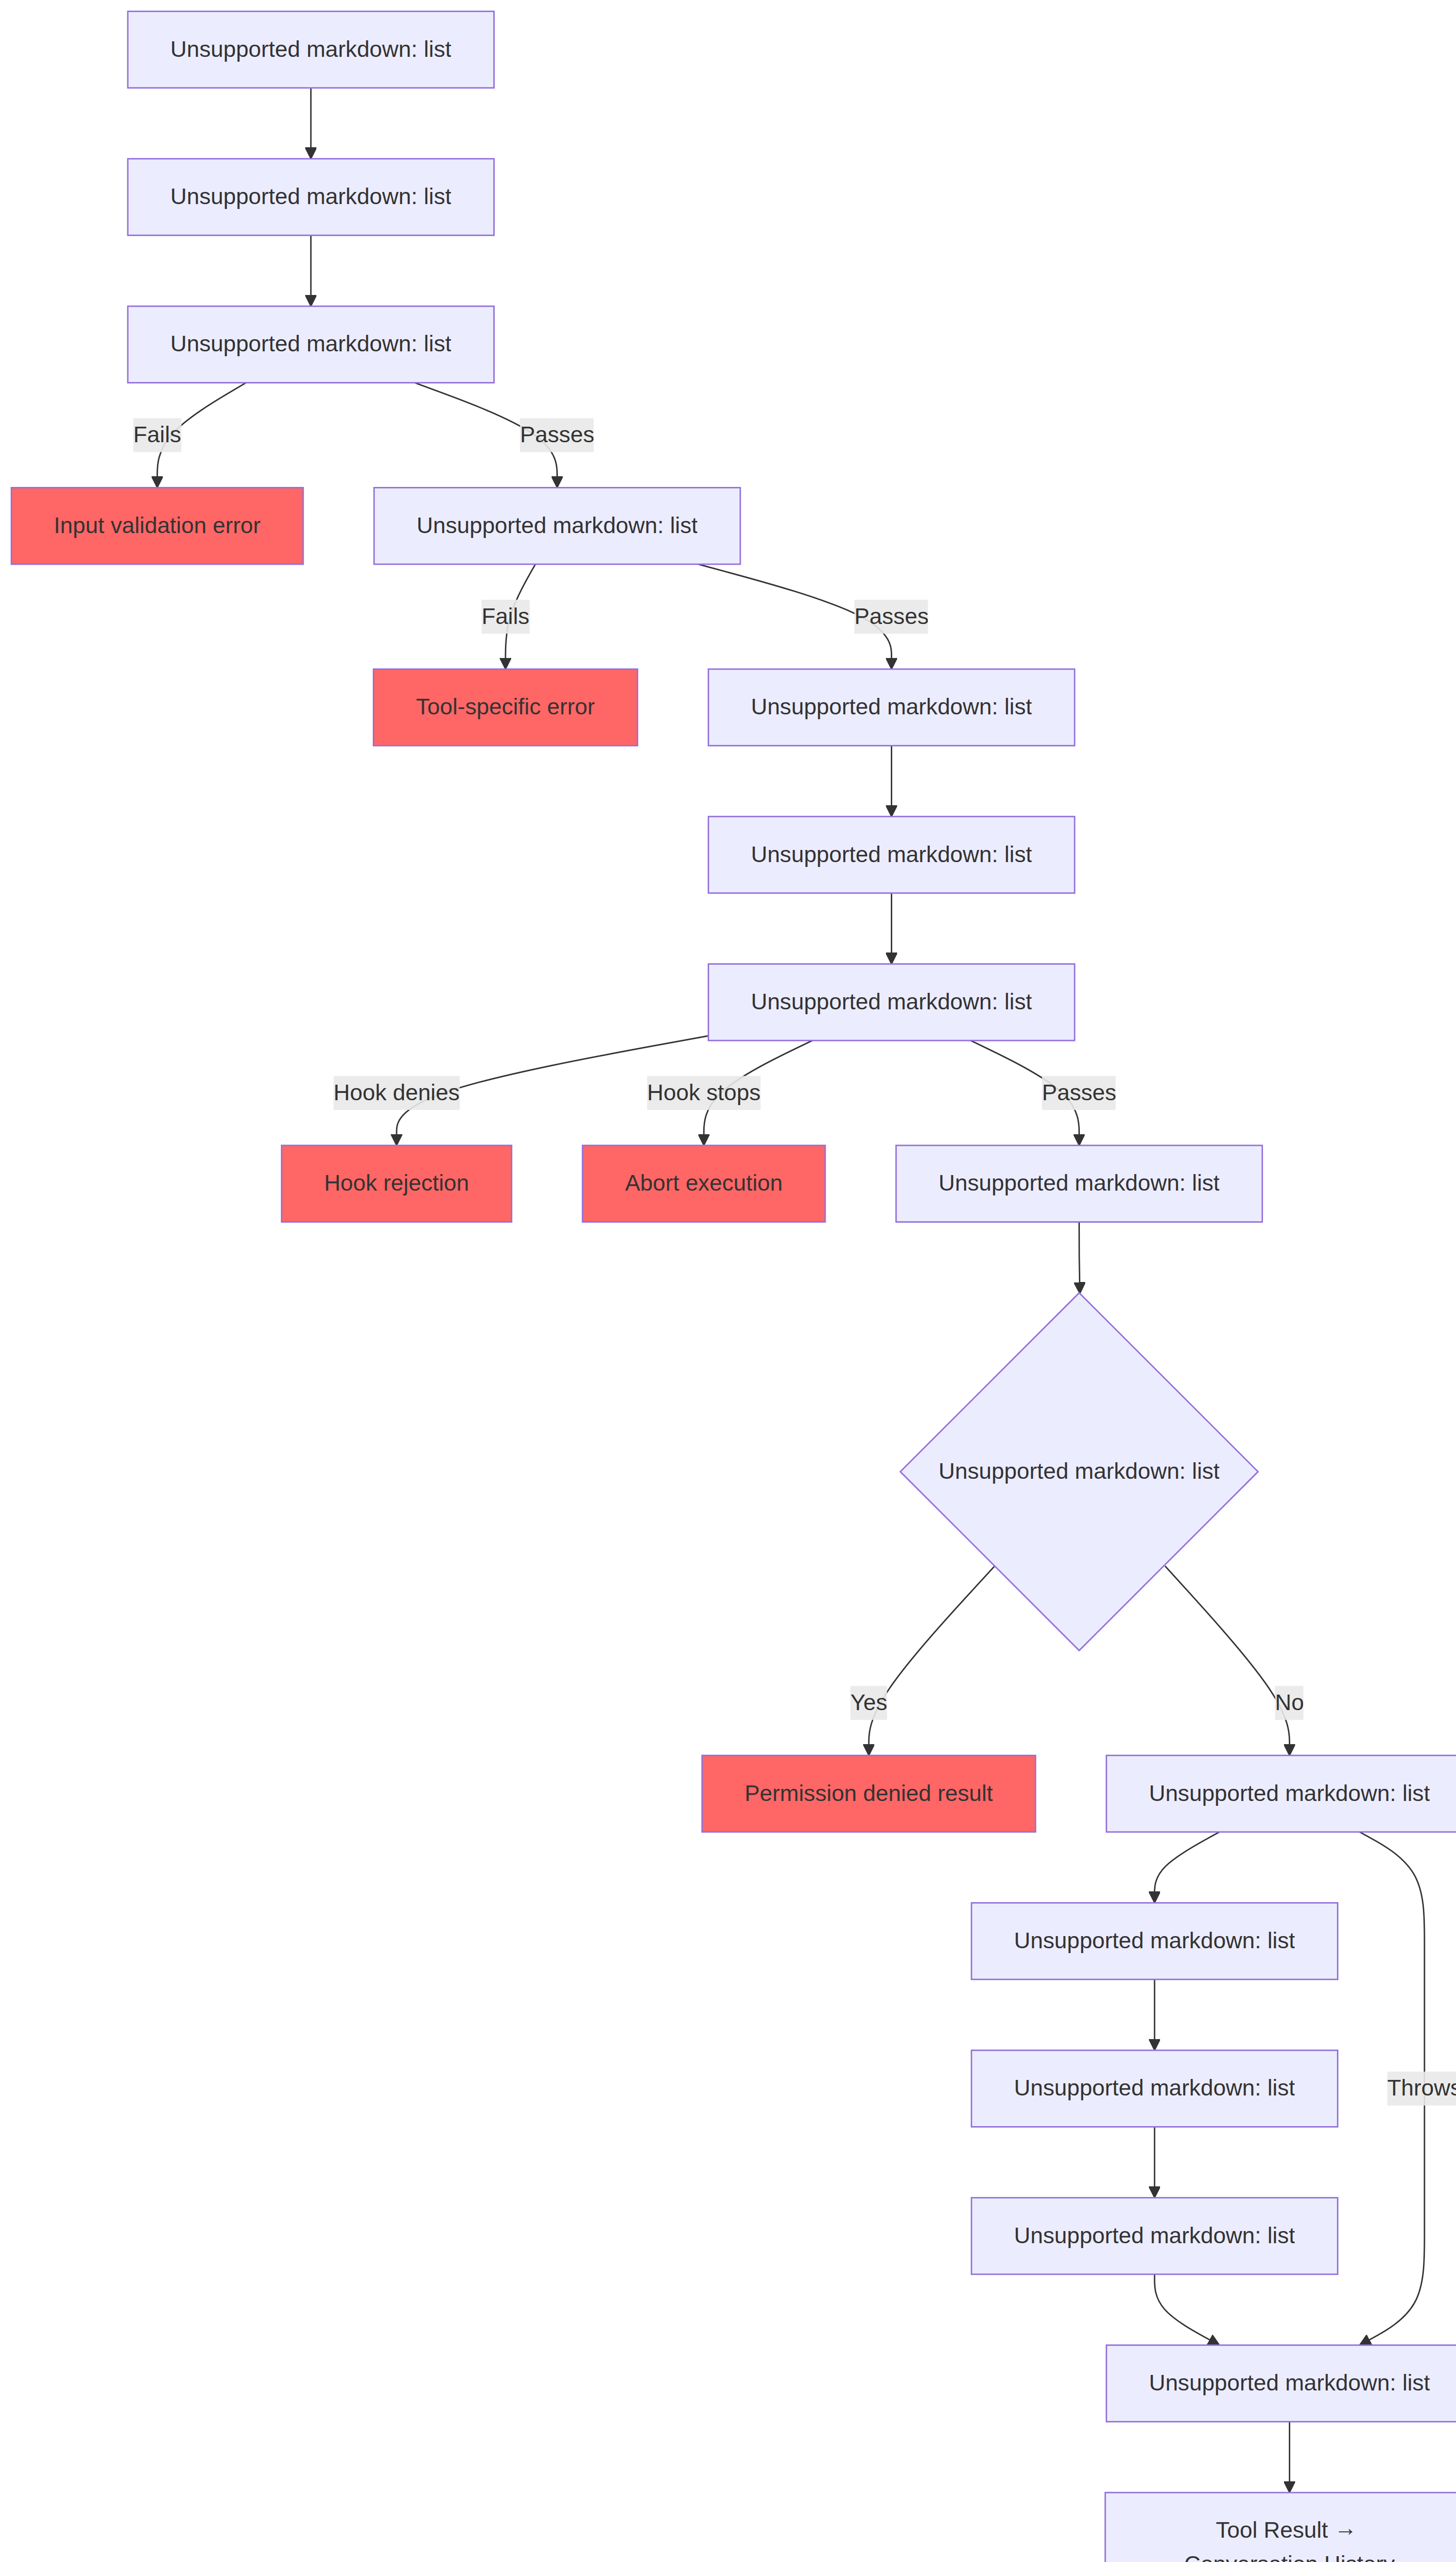
\includegraphics[width=10.91in,height=19.21in]{book/ch06-tools_files/figure-latex/mermaid-figure-1.png}

\subsection{Steps 1-4: Validation}\label{steps-1-4-validation}

\textbf{Tool Lookup} falls back to \texttt{getAllBaseTools()} for alias
matches, handling transcripts from older sessions where a tool was
renamed. \textbf{Abort Check} prevents wasted computation on tool calls
queued before Ctrl+C propagated. \textbf{Zod Validation} catches type
mismatches; for deferred tools, the error appends a hint to call
ToolSearch first. \textbf{Semantic Validation} goes beyond schema
conformance -- FileEditTool rejects no-op edits, BashTool blocks
standalone \texttt{sleep} when MonitorTool is available.

\subsection{Steps 5-6: Preparation}\label{steps-5-6-preparation}

\textbf{Speculative Classifier Start} kicks off the auto-mode security
classifier in parallel for Bash commands, shaving hundreds of
milliseconds off the common path. \textbf{Input Backfill} clones the
parsed input and adds derived fields (expanding
\texttt{\textasciitilde{}/foo.txt} to absolute paths) for hooks and
permissions, preserving the original for transcript stability.

\subsection{Steps 7-9: Permission}\label{steps-7-9-permission}

\textbf{PreToolUse Hooks} are the extension mechanism -- they can make
permission decisions, modify inputs, inject context, or stop execution
entirely. \textbf{Permission Resolution} bridges hooks and the general
permission system: if a hook already decided, that is final; otherwise
\texttt{canUseTool()} triggers rule matching, tool-specific checks,
mode-based defaults, and interactive prompts. \textbf{Permission Denied
Handling} builds an error message and executes \texttt{PermissionDenied}
hooks.

\subsection{Steps 10-14: Execution and
Cleanup}\label{steps-10-14-execution-and-cleanup}

\textbf{Tool Execution} runs the actual \texttt{call()} with the
original input. \textbf{Result Budgeting} persists oversized output to
\texttt{\textasciitilde{}/.claude/tool-results/\{hash\}.txt} and
replaces it with a preview. \textbf{PostToolUse Hooks} can modify MCP
output or block continuation. \textbf{New Messages} are appended
(sub-agent transcripts, system reminders). \textbf{Error Handling}
classifies errors for telemetry, extracts safe strings from potentially
mangled names, and emits OTel events.

\begin{center}\rule{0.5\linewidth}{0.5pt}\end{center}

\section{The Permission System}\label{the-permission-system-1}

\subsection{Seven Modes}\label{seven-modes}

\begin{longtable}[]{@{}
  >{\raggedright\arraybackslash}p{(\linewidth - 2\tabcolsep) * \real{0.3750}}
  >{\raggedright\arraybackslash}p{(\linewidth - 2\tabcolsep) * \real{0.6250}}@{}}
\toprule\noalign{}
\begin{minipage}[b]{\linewidth}\raggedright
Mode
\end{minipage} & \begin{minipage}[b]{\linewidth}\raggedright
Behavior
\end{minipage} \\
\midrule\noalign{}
\endhead
\bottomrule\noalign{}
\endlastfoot
\texttt{default} & Tool-specific checks; prompt user for unrecognized
operations \\
\texttt{acceptEdits} & Auto-allow file edits; prompt for other
operations \\
\texttt{plan} & Read-only -- deny all write operations \\
\texttt{dontAsk} & Auto-deny anything that would normally prompt
(background agents) \\
\texttt{bypassPermissions} & Allow everything without prompting \\
\texttt{auto} & Use the transcript classifier to decide
(feature-flagged) \\
\texttt{bubble} & Internal mode for sub-agents that escalate to the
parent \\
\end{longtable}

\subsection{The Resolution Chain}\label{the-resolution-chain}

When a tool call reaches permission resolution:

\begin{enumerate}
\def\labelenumi{\arabic{enumi}.}
\tightlist
\item
  \textbf{Hook decision}: If a PreToolUse hook already returned
  \texttt{allow} or \texttt{deny}, that is final.
\item
  \textbf{Rule matching}: Three rule sets -- \texttt{alwaysAllowRules},
  \texttt{alwaysDenyRules}, \texttt{alwaysAskRules} -- match on tool
  name and optional content patterns. \texttt{Bash(git\ *)} matches any
  Bash command starting with \texttt{git}.
\item
  \textbf{Tool-specific check}: The tool's \texttt{checkPermissions()}
  method. Most return \texttt{passthrough}.
\item
  \textbf{Mode-based default}: \texttt{bypassPermissions} allows
  everything. \texttt{plan} denies writes. \texttt{dontAsk} denies
  prompts.
\item
  \textbf{Interactive prompt}: In \texttt{default} and
  \texttt{acceptEdits} modes, unresolved decisions show a prompt.
\item
  \textbf{Auto-mode classifier}: A two-stage classifier (fast model,
  then extended thinking for ambiguous cases).
\end{enumerate}

The \texttt{safetyCheck} variant has a \texttt{classifierApprovable}
boolean: \texttt{.claude/} and \texttt{.git/} edits are
\texttt{classifierApprovable:\ true} (unusual but sometimes legitimate),
while Windows path bypass attempts are
\texttt{classifierApprovable:\ false} (almost always adversarial).

\subsection{Permission Rules and
Matching}\label{permission-rules-and-matching}

Permission rules are stored as \texttt{PermissionRule} objects with
three parts: a \texttt{source} tracing provenance (userSettings,
projectSettings, localSettings, cliArg, policySettings, session, etc.),
a \texttt{ruleBehavior} (allow, deny, ask), and a \texttt{ruleValue}
with the tool name and optional content pattern.

The \texttt{ruleContent} field enables fine-grained matching.
\texttt{Bash(git\ *)} allows any Bash command starting with
\texttt{git}. \texttt{Edit(/src/**)} allows edits only within
\texttt{/src}. \texttt{Fetch(domain:example.com)} allows fetching from a
specific domain. Rules without \texttt{ruleContent} match all
invocations of that tool.

BashTool's permission matcher parses the command via
\texttt{parseForSecurity()} (a bash AST parser) and splits compound
commands into subcommands. If AST parsing fails (complex syntax with
heredocs or nested subshells), the matcher returns
\texttt{()\ =\textgreater{}\ true} -- fail-safe, meaning the hook always
runs. The assumption is that if the command is too complex to parse, it
is too complex to confidently exclude from safety checks.

\subsection{Bubble Mode for
Sub-Agents}\label{bubble-mode-for-sub-agents}

Sub-agents in coordinator-worker patterns cannot show permission prompts
-- they have no terminal. The \texttt{bubble} mode causes permission
requests to propagate up to the parent context. The coordinator agent,
running in the main thread with terminal access, handles the prompt and
sends the decision back down.

\begin{center}\rule{0.5\linewidth}{0.5pt}\end{center}

\section{Tool Deferred Loading}\label{tool-deferred-loading}

Tools with \texttt{shouldDefer:\ true} are sent to the API with
\texttt{defer\_loading:\ true} -- names and descriptions but not full
parameter schemas. This reduces initial prompt size. To use a deferred
tool, the model must first call \texttt{ToolSearchTool} to load its
schema. The failure mode is instructive: calling a deferred tool without
loading it causes Zod validation to fail (all typed parameters arrive as
strings), and the system appends a targeted recovery hint.

Deferred loading also improves cache hit rates: tools sent with
\texttt{defer\_loading:\ true} contribute only their name to the prompt,
so adding or removing a deferred MCP tool changes the prompt by a few
tokens rather than hundreds.

\begin{center}\rule{0.5\linewidth}{0.5pt}\end{center}

\section{Result Budgeting}\label{result-budgeting}

\subsection{Per-Tool Size Limits}\label{per-tool-size-limits}

Each tool declares \texttt{maxResultSizeChars}:

\begin{longtable}[]{@{}
  >{\raggedright\arraybackslash}p{(\linewidth - 4\tabcolsep) * \real{0.1667}}
  >{\raggedright\arraybackslash}p{(\linewidth - 4\tabcolsep) * \real{0.5278}}
  >{\raggedright\arraybackslash}p{(\linewidth - 4\tabcolsep) * \real{0.3056}}@{}}
\toprule\noalign{}
\begin{minipage}[b]{\linewidth}\raggedright
Tool
\end{minipage} & \begin{minipage}[b]{\linewidth}\raggedright
maxResultSizeChars
\end{minipage} & \begin{minipage}[b]{\linewidth}\raggedright
Rationale
\end{minipage} \\
\midrule\noalign{}
\endhead
\bottomrule\noalign{}
\endlastfoot
BashTool & 30,000 & Enough for most useful output \\
FileEditTool & 100,000 & Diffs can be large but the model needs them \\
GrepTool & 100,000 & Search results with context lines add up fast \\
FileReadTool & Infinity & Self-bounds via its own token limits;
persisting would create circular Read loops \\
\end{longtable}

When a result exceeds the threshold, the full content is saved to disk
and replaced with a \texttt{\textless{}persisted-output\textgreater{}}
wrapper containing a preview and file path. The model can then use
\texttt{Read} to access the full output if needed.

\subsection{Per-Conversation Aggregate
Budget}\label{per-conversation-aggregate-budget}

Beyond per-tool limits, \texttt{ContentReplacementState} tracks an
aggregate budget across the entire conversation, preventing death by a
thousand cuts -- many tools each returning 90\% of their individual
limit can still overwhelm the context window.

\begin{center}\rule{0.5\linewidth}{0.5pt}\end{center}

\section{Individual Tool Highlights}\label{individual-tool-highlights}

\subsection{BashTool: The Most Complex
Tool}\label{bashtool-the-most-complex-tool}

BashTool is the system's most complex tool by far. It parses compound
commands, classifies subcommands as read-only or write, manages
background tasks, detects image output by magic bytes, and implements a
sed simulation for safe edit previews.

The compound command parsing is particularly interesting.
\texttt{splitCommandWithOperators()} breaks a command like
\texttt{cd\ /tmp\ \&\&\ mkdir\ build\ \&\&\ ls\ build} into individual
subcommands. Each is classified against known-safe command sets
(\texttt{BASH\_SEARCH\_COMMANDS}, \texttt{BASH\_READ\_COMMANDS},
\texttt{BASH\_LIST\_COMMANDS}). A compound command is read-only only if
ALL non-neutral parts are safe. The neutral set (echo, printf) is
ignored -- they do not make a command read-only, but they also do not
make it write-only.

The sed simulation (\texttt{\_simulatedSedEdit}) deserves special
attention. When a user approves a sed command in the permission dialog,
the system pre-computes the result by running the sed command in a
sandbox and capturing the output. The pre-computed result is injected
into the input as \texttt{\_simulatedSedEdit}. When \texttt{call()}
executes, it applies the edit directly, bypassing shell execution. This
guarantees that what the user previewed is exactly what gets written --
not a re-execution that might produce different results if the file
changed between preview and execution.

\subsection{FileEditTool: Staleness
Detection}\label{fileedittool-staleness-detection}

FileEditTool integrates with \texttt{readFileState}, the LRU cache of
file contents and timestamps maintained across the conversation. Before
applying an edit, it checks whether the file has been modified since the
model last read it. If the file is stale -- modified by a background
process, another tool, or the user -- the edit is rejected with a
message telling the model to re-read the file first.

The fuzzy matching in \texttt{findActualString()} handles the common
case where the model gets whitespace slightly wrong. It normalizes
whitespace and quote styles before matching, so an edit targeting
\texttt{old\_string} with trailing spaces still matches the file's
actual content. The \texttt{replace\_all} flag enables bulk
replacements; without it, non-unique matches are rejected, requiring the
model to provide enough context to identify a single location.

\subsection{FileReadTool: The Versatile
Reader}\label{filereadtool-the-versatile-reader}

FileReadTool is the only built-in tool with
\texttt{maxResultSizeChars:\ Infinity}. If Read output were persisted to
disk, the model would need to Read the persisted file, which could
itself exceed the limit, creating an infinite loop. The tool instead
self-bounds via token estimation and truncates at the source.

The tool is remarkably versatile: it reads text files with line numbers,
images (returning base64 multimodal content blocks), PDFs (via
\texttt{extractPDFPages()}), Jupyter notebooks (via
\texttt{readNotebook()}), and directories (falling back to \texttt{ls}).
It blocks dangerous device paths (\texttt{/dev/zero},
\texttt{/dev/random}, \texttt{/dev/stdin}) and handles macOS screenshot
filename quirks (U+202F narrow no-break space vs regular space in
``Screen Shot'' filenames).

\subsection{GrepTool: Pagination via
head\_limit}\label{greptool-pagination-via-head_limit}

GrepTool wraps \texttt{ripGrep()} and adds a pagination mechanism via
\texttt{head\_limit}. The default is 250 entries -- enough for useful
results but small enough to avoid context bloat. When truncation occurs,
the response includes \texttt{appliedLimit:\ 250}, signaling the model
to use \texttt{offset} on the next call to paginate. An explicit
\texttt{head\_limit:\ 0} disables the limit entirely.

GrepTool automatically excludes six VCS directories (\texttt{.git},
\texttt{.svn}, \texttt{.hg}, \texttt{.bzr}, \texttt{.jj}, \texttt{.sl}).
Searching inside \texttt{.git/objects} is almost never what the model
wants, and accidental inclusion of binary pack files would blow through
token budgets.

\subsection{AgentTool and Context
Modifiers}\label{agenttool-and-context-modifiers}

AgentTool spawns sub-agents that run their own query loops. Its
\texttt{call()} returns \texttt{newMessages} containing the sub-agent's
transcript, and optionally a \texttt{contextModifier} that propagates
state changes back to the parent. Because AgentTool is not
concurrency-safe by default, multiple Agent tool calls in a single
response run serially -- each sub-agent's context modifier is applied
before the next sub-agent starts. In coordinator mode, the pattern
inverts: the coordinator dispatches sub-agents for independent tasks,
and the \texttt{isAgentSwarmsEnabled()} check unlocks parallel agent
execution.

\begin{center}\rule{0.5\linewidth}{0.5pt}\end{center}

\section{How Tools Interact with the Message
History}\label{how-tools-interact-with-the-message-history}

Tool results do not simply return data to the model. They participate in
the conversation as structured messages.

The API expects tool results as \texttt{ToolResultBlockParam} objects
that reference the original \texttt{tool\_use} block by ID. Most tools
serialize to text. FileReadTool can serialize to image content blocks
(base64-encoded) for multimodal responses. BashTool detects image output
by inspecting magic bytes in stdout and switches to image blocks
accordingly.

\texttt{ToolResult.newMessages} is how tools extend the conversation
beyond the simple call-and-response pattern. \textbf{Agent transcripts}:
AgentTool injects the sub-agent's message history as attachment
messages. \textbf{System reminders}: Memory tools inject system messages
that appear after the tool result -- visible to the model on the next
turn but stripped at the \texttt{normalizeMessagesForAPI} boundary.
\textbf{Attachment messages}: Hook results, additional context, and
error details carry structured metadata that the model can reference in
subsequent turns.

The \texttt{contextModifier} function is the mechanism for tools that
change the execution environment. When \texttt{EnterPlanMode} executes,
it returns a modifier that sets the permission mode to
\texttt{\textquotesingle{}plan\textquotesingle{}}. When
\texttt{ExitWorktree} executes, it modifies the working directory. These
modifiers are the only way for a tool to affect subsequent tools --
direct mutation of \texttt{ToolUseContext} is not possible because the
context is spread-copied before each tool call. The serial-only
restriction is enforced by the orchestration layer: if two concurrent
tools both modify the working directory, which wins?

\begin{center}\rule{0.5\linewidth}{0.5pt}\end{center}

\section{Apply This: Designing a Tool
System}\label{apply-this-designing-a-tool-system}

\textbf{Fail-closed defaults.} New tools should be conservative until
explicitly marked otherwise. A developer who forgets to set a flag gets
the safe behavior, not the dangerous one.

\textbf{Input-dependent safety.} \texttt{isConcurrencySafe(input)} and
\texttt{isReadOnly(input)} take the parsed input because the same tool
at different inputs has different safety profiles. A tool registry that
marks BashTool as ``always serial'' is correct but wasteful.

\textbf{Layer your permissions.} Tool-specific checks, rule-based
matching, mode-based defaults, interactive prompts, and automated
classifiers each handle different cases. No single mechanism is
sufficient.

\textbf{Budget results, not just inputs.} Token limits on input are
standard. But tool results can be arbitrarily large and they accumulate
across turns. Per-tool limits prevent individual explosions. Aggregate
conversation limits prevent cumulative overflow.

\textbf{Make error classification telemetry-safe.} In minified builds,
\texttt{error.constructor.name} is mangled. The
\texttt{classifyToolError()} function extracts the most informative safe
string available -- telemetry-safe messages, errno codes, stable error
names -- without ever logging the raw error message to analytics.

\begin{center}\rule{0.5\linewidth}{0.5pt}\end{center}

\section{What Comes Next}\label{what-comes-next}

This chapter traced how a single tool call flows from definition through
validation, permission, execution, and result budgeting. But the model
rarely requests just one tool at a time. How tools are orchestrated into
concurrent batches is the subject of Chapter 7.

\chapter{Chapter 7: Concurrent Tool
Execution}\label{chapter-7-concurrent-tool-execution}

\section{The Cost of Waiting}\label{the-cost-of-waiting}

Chapter 6 traced the lifecycle of a single tool call -- from the raw
\texttt{tool\_use} block in the API response through input validation,
permission checks, execution, and result formatting. That pipeline
handles one tool. But the model rarely requests just one.

A typical Claude Code interaction involves three to five tool calls per
turn. ``Read these two files, grep for this pattern, then edit this
function.'' The model emits all of those in a single response. If each
tool takes 200 milliseconds, running them sequentially costs a full
second. If the Read and Grep calls are independent -- and they are --
running them in parallel cuts that to 200 milliseconds. Five-to-one
improvement, free.

But not all tools are independent. An Edit that modifies
\texttt{config.ts} cannot run concurrently with another Edit that
modifies \texttt{config.ts}. A Bash command that creates a directory
must complete before a Bash command that writes a file into that
directory. Concurrency is not a global property of a tool. It is a
property of a specific tool invocation with specific inputs.

This is the insight that drives the entire concurrency system:
\textbf{safety is per-call, not per-tool-type}. \texttt{Bash("ls\ -la")}
is safe to parallelize. \texttt{Bash("rm\ -rf\ build/")} is not. The
same tool, different inputs, different concurrency classification. The
system must inspect the input before deciding.

Claude Code implements two layers of concurrency optimization. The first
is \textbf{batch orchestration}: after the model's response is fully
received, partition the tool calls into concurrent and serial groups,
then execute each group appropriately. The second is \textbf{speculative
execution}: start running tools \emph{while the model is still streaming
its response}, harvesting results before the response is even complete.
Together, these two mechanisms eliminate most of the wall-clock time
that would otherwise be spent waiting.

\begin{center}\rule{0.5\linewidth}{0.5pt}\end{center}

\section{The Partition Algorithm}\label{the-partition-algorithm}

The entry point is \texttt{partitionToolCalls()} in
\texttt{toolOrchestration.ts}. It takes an ordered array of
\texttt{ToolUseBlock} messages and produces an array of batches, where
each batch is either ``all concurrent-safe'' or ``a single serial
tool.''

\begin{Shaded}
\begin{Highlighting}[]
\CommentTok{// Pseudocode — illustrates the partition algorithm}
\KeywordTok{type}\NormalTok{ Group }\OperatorTok{=}\NormalTok{ \{ parallel}\OperatorTok{:} \DataTypeTok{boolean}\OperatorTok{;}\NormalTok{ calls}\OperatorTok{:}\NormalTok{ ToolCall[] \}}

\KeywordTok{function} \FunctionTok{groupBySafety}\NormalTok{(calls}\OperatorTok{:}\NormalTok{ ToolCall[]}\OperatorTok{,}\NormalTok{ registry}\OperatorTok{:}\NormalTok{ ToolRegistry)}\OperatorTok{:}\NormalTok{ Group[] \{}
  \ControlFlowTok{return}\NormalTok{ calls}\OperatorTok{.}\FunctionTok{reduce}\NormalTok{((groups}\OperatorTok{,}\NormalTok{ call) }\KeywordTok{=\textgreater{}}\NormalTok{ \{}
    \KeywordTok{const}\NormalTok{ def }\OperatorTok{=}\NormalTok{ registry}\OperatorTok{.}\FunctionTok{lookup}\NormalTok{(call}\OperatorTok{.}\AttributeTok{name}\NormalTok{)}
    \KeywordTok{const}\NormalTok{ input }\OperatorTok{=}\NormalTok{ def}\OperatorTok{?.}\AttributeTok{schema}\OperatorTok{.}\FunctionTok{safeParse}\NormalTok{(call}\OperatorTok{.}\AttributeTok{input}\NormalTok{)}
    \CommentTok{// Fail{-}closed: parse failure or exception → serial}
    \KeywordTok{const}\NormalTok{ safe }\OperatorTok{=}\NormalTok{ input}\OperatorTok{?.}\AttributeTok{success}
      \OperatorTok{?} \FunctionTok{tryCatch}\NormalTok{(() }\KeywordTok{=\textgreater{}}\NormalTok{ def}\OperatorTok{.}\FunctionTok{isParallelSafe}\NormalTok{(input}\OperatorTok{.}\AttributeTok{data}\NormalTok{)}\OperatorTok{,} \KeywordTok{false}\NormalTok{)}
      \OperatorTok{:} \KeywordTok{false}
    \CommentTok{// Merge consecutive safe calls into one group}
    \ControlFlowTok{if}\NormalTok{ (safe }\OperatorTok{\&\&}\NormalTok{ groups}\OperatorTok{.}\FunctionTok{at}\NormalTok{(}\OperatorTok{{-}}\DecValTok{1}\NormalTok{)}\OperatorTok{?.}\AttributeTok{parallel}\NormalTok{) \{}
\NormalTok{      groups}\OperatorTok{.}\FunctionTok{at}\NormalTok{(}\OperatorTok{{-}}\DecValTok{1}\NormalTok{)}\OperatorTok{!.}\AttributeTok{calls}\OperatorTok{.}\FunctionTok{push}\NormalTok{(call)}
\NormalTok{    \} }\ControlFlowTok{else}\NormalTok{ \{}
\NormalTok{      groups}\OperatorTok{.}\FunctionTok{push}\NormalTok{(\{ parallel}\OperatorTok{:}\NormalTok{ safe}\OperatorTok{,}\NormalTok{ calls}\OperatorTok{:}\NormalTok{ [call] \})}
\NormalTok{    \}}
    \ControlFlowTok{return}\NormalTok{ groups}
\NormalTok{  \}}\OperatorTok{,}\NormalTok{ [] }\ImportTok{as}\NormalTok{ Group[])}
\NormalTok{\}}
\end{Highlighting}
\end{Shaded}

The algorithm walks the array left to right. For each tool call:

\begin{enumerate}
\def\labelenumi{\arabic{enumi}.}
\tightlist
\item
  \textbf{Look up the tool definition} by name.
\item
  \textbf{Parse the input} with the tool's Zod schema via
  \texttt{safeParse()}. If parsing fails, the tool is conservatively
  classified as not concurrency-safe.
\item
  \textbf{Call \texttt{isConcurrencySafe(parsedInput)}} on the tool
  definition. This is where per-input classification happens. The Bash
  tool parses the command string, checks if every subcommand is
  read-only (\texttt{ls}, \texttt{grep}, \texttt{cat},
  \texttt{git\ status}), and returns \texttt{true} only if the entire
  compound command is a pure read. The Read tool always returns
  \texttt{true}. The Edit tool always returns \texttt{false}. The call
  is wrapped in try-catch -- if \texttt{isConcurrencySafe} throws (say,
  the Bash command string can't be parsed by the shell-quote library),
  the tool defaults to serial.
\item
  \textbf{Merge or create a batch.} If the current tool is
  concurrency-safe AND the most recent batch is also concurrency-safe,
  append to that batch. Otherwise, start a new batch.
\end{enumerate}

The result is a sequence of batches that alternates between concurrent
groups and individual serial entries. Walk through a concrete example:

\begin{verbatim}
Model requests: [Read, Read, Grep, Edit, Read]

Step 1: Read  → concurrent-safe → new batch {safe, [Read]}
Step 2: Read  → concurrent-safe → append   {safe, [Read, Read]}
Step 3: Grep  → concurrent-safe → append   {safe, [Read, Read, Grep]}
Step 4: Edit  → NOT safe        → new batch {serial, [Edit]}
Step 5: Read  → concurrent-safe → new batch {safe, [Read]}

Result: 3 batches
  Batch 1: [Read, Read, Grep]  — run concurrently
  Batch 2: [Edit]              — run alone
  Batch 3: [Read]              — run concurrently (just one tool)
\end{verbatim}

The partitioning is greedy and order-preserving. Consecutive safe tools
accumulate into a single batch. Any unsafe tool breaks the run and
starts a new batch. This means the order in which the model emits tool
calls matters -- if it interleaves a Write between two Reads, you get
three batches instead of two. In practice, models tend to cluster their
reads together, which is the common case the algorithm is optimized for.

\begin{center}\rule{0.5\linewidth}{0.5pt}\end{center}

\section{Batch Execution}\label{batch-execution}

The \texttt{runTools()} generator iterates through the partitioned
batches and dispatches each one to the appropriate executor.

\subsection{Concurrent Batches}\label{concurrent-batches}

For a concurrent batch, \texttt{runToolsConcurrently()} fires all tools
in parallel using an \texttt{all()} utility that caps active generators
at the concurrency limit:

\begin{Shaded}
\begin{Highlighting}[]
\CommentTok{// Pseudocode — illustrates the concurrent dispatch pattern}
\KeywordTok{async} \KeywordTok{function}\OperatorTok{*} \FunctionTok{dispatchParallel}\NormalTok{(calls}\OperatorTok{,}\NormalTok{ context) \{}
  \KeywordTok{yield}\OperatorTok{*} \FunctionTok{boundedAll}\NormalTok{(}
\NormalTok{    calls}\OperatorTok{.}\FunctionTok{map}\NormalTok{(}\KeywordTok{async} \KeywordTok{function}\OperatorTok{*}\NormalTok{ (call) \{}
\NormalTok{      context}\OperatorTok{.}\FunctionTok{markInProgress}\NormalTok{(call}\OperatorTok{.}\AttributeTok{id}\NormalTok{)}
      \KeywordTok{yield}\OperatorTok{*} \FunctionTok{executeSingle}\NormalTok{(call}\OperatorTok{,}\NormalTok{ context)}
\NormalTok{      context}\OperatorTok{.}\FunctionTok{markComplete}\NormalTok{(call}\OperatorTok{.}\AttributeTok{id}\NormalTok{)}
\NormalTok{    \})}\OperatorTok{,}
\NormalTok{    MAX\_CONCURRENCY}\OperatorTok{,}  \CommentTok{// Default: 10}
\NormalTok{  )}
\NormalTok{\}}
\end{Highlighting}
\end{Shaded}

The concurrency limit defaults to 10, configurable via
\texttt{CLAUDE\_CODE\_MAX\_TOOL\_USE\_CONCURRENCY}. Ten is generous --
you rarely see more than five or six tool calls in a single model
response. The limit exists as a safety valve for pathological cases, not
as a typical constraint.

The \texttt{all()} utility is a generator-aware variant of
\texttt{Promise.all} with bounded concurrency. It starts up to N
generators simultaneously, yields results from whichever completes
first, and starts the next queued generator as each one finishes. The
mechanics are similar to a semaphore-guarded task pool, but adapted for
async generators that yield intermediate results.

\textbf{Context modifier queuing} is the subtle part. Some tools produce
\emph{context modifiers} -- functions that transform the
\texttt{ToolUseContext} for subsequent tools. When tools run
concurrently, you cannot apply these modifiers immediately because other
tools in the same batch are reading the same context. Instead, modifiers
are collected in a map keyed by tool use ID:

\begin{Shaded}
\begin{Highlighting}[]
\KeywordTok{const}\NormalTok{ queuedContextModifiers}\OperatorTok{:} \BuiltInTok{Record}\OperatorTok{\textless{}}
\NormalTok{  string}\OperatorTok{,}
\NormalTok{  ((context}\OperatorTok{:}\NormalTok{ ToolUseContext) }\KeywordTok{=\textgreater{}}\NormalTok{ ToolUseContext)[]}
\OperatorTok{\textgreater{}} \OperatorTok{=}\NormalTok{ \{\}}
\end{Highlighting}
\end{Shaded}

After the entire concurrent batch finishes, the modifiers are applied in
tool-order (not completion-order), preserving deterministic context
evolution:

\begin{Shaded}
\begin{Highlighting}[]
\ControlFlowTok{for}\NormalTok{ (}\KeywordTok{const}\NormalTok{ block }\KeywordTok{of}\NormalTok{ blocks) \{}
  \KeywordTok{const}\NormalTok{ modifiers }\OperatorTok{=}\NormalTok{ queuedContextModifiers[block}\OperatorTok{.}\AttributeTok{id}\NormalTok{]}
  \ControlFlowTok{if}\NormalTok{ (}\OperatorTok{!}\NormalTok{modifiers) }\ControlFlowTok{continue}
  \ControlFlowTok{for}\NormalTok{ (}\KeywordTok{const}\NormalTok{ modifier }\KeywordTok{of}\NormalTok{ modifiers) \{}
\NormalTok{    currentContext }\OperatorTok{=} \FunctionTok{modifier}\NormalTok{(currentContext)}
\NormalTok{  \}}
\NormalTok{\}}
\end{Highlighting}
\end{Shaded}

In practice, none of the current concurrency-safe tools produce context
modifiers -- the comment in the codebase acknowledges this explicitly.
But the infrastructure exists because tools can be added by MCP servers,
and a custom read-only MCP tool might legitimately want to modify
context (updating a ``files seen'' set, for instance).

\subsection{Serial Batches}\label{serial-batches}

Serial execution is straightforward. Each tool runs, its context
modifiers are applied immediately, and the next tool sees the updated
context:

\begin{Shaded}
\begin{Highlighting}[]
\ControlFlowTok{for}\NormalTok{ (}\KeywordTok{const}\NormalTok{ toolUse }\KeywordTok{of}\NormalTok{ toolUseMessages) \{}
  \ControlFlowTok{for} \ControlFlowTok{await}\NormalTok{ (}\KeywordTok{const}\NormalTok{ update }\KeywordTok{of} \FunctionTok{runToolUse}\NormalTok{(toolUse}\OperatorTok{,} \CommentTok{/* ... */}\NormalTok{)) \{}
    \ControlFlowTok{if}\NormalTok{ (update}\OperatorTok{.}\AttributeTok{contextModifier}\NormalTok{) \{}
\NormalTok{      currentContext }\OperatorTok{=}\NormalTok{ update}\OperatorTok{.}\AttributeTok{contextModifier}\OperatorTok{.}\FunctionTok{modifyContext}\NormalTok{(currentContext)}
\NormalTok{    \}}
    \KeywordTok{yield}\NormalTok{ \{ message}\OperatorTok{:}\NormalTok{ update}\OperatorTok{.}\AttributeTok{message}\OperatorTok{,}\NormalTok{ newContext}\OperatorTok{:}\NormalTok{ currentContext \}}
\NormalTok{  \}}
\NormalTok{\}}
\end{Highlighting}
\end{Shaded}

This is the critical difference. Serial tools can change the world for
subsequent tools. An Edit modifies a file; the next Read sees the
modified version. A Bash command creates a directory; the next Bash
command writes into it. Context modifiers are the formalization of this
dependency: they let a tool say ``the execution environment has changed,
here's how.''

\begin{center}\rule{0.5\linewidth}{0.5pt}\end{center}

\section{The Streaming Tool Executor}\label{the-streaming-tool-executor}

Batch orchestration eliminates unnecessary serialization \emph{after}
the model's response arrives. But there is a bigger opportunity: the
model's response takes time to stream. A typical multi-tool response
might take 2-3 seconds to fully arrive. The first tool call is parseable
after 500 milliseconds. Why wait for the remaining 2 seconds?

The \texttt{StreamingToolExecutor} class implements speculative
execution. As the model streams its response, each \texttt{tool\_use}
block is handed to the executor the moment it is fully parsed. The
executor starts running it immediately -- while the model is still
generating the next tool call. By the time the response finishes
streaming, several tools may have already completed.

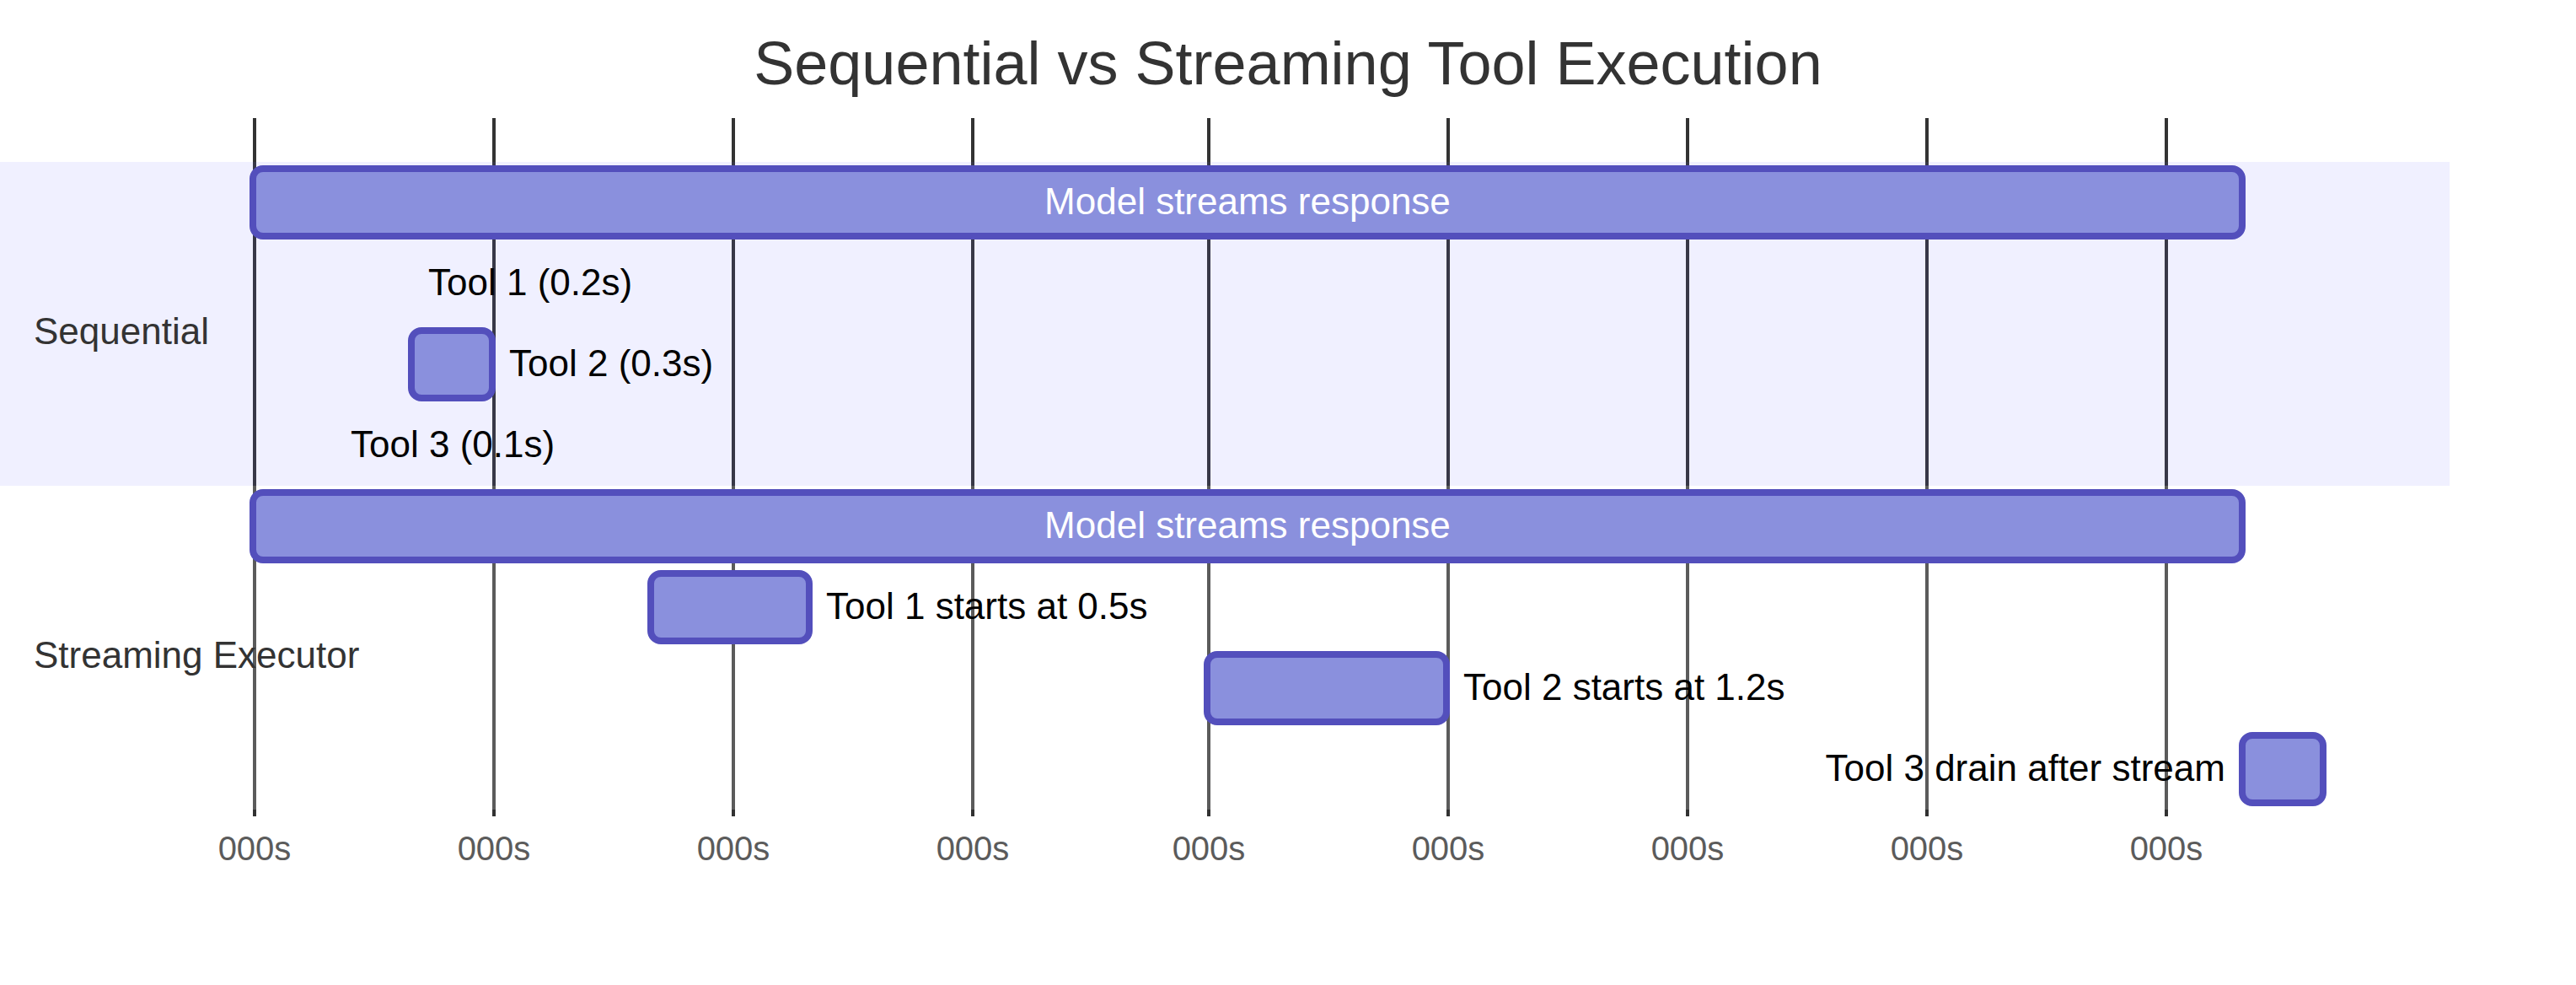
\includegraphics[width=7.96in,height=3.04in]{book/ch07-concurrency_files/figure-latex/mermaid-figure-1.png}

Sequential total: 3.1s. Streaming total: 2.6s -- tools 1 and 2 completed
during streaming, saving 16\% of wall-clock time.

The savings compound. When the model requests five read-only tools and
the response takes 3 seconds to stream, all five tools can start and
finish during that 3 seconds. The post-stream drain phase has nothing
left to do. The user sees results almost immediately after the last
character of the model's response appears.

\subsection{Tool Lifecycle}\label{tool-lifecycle}

Each tool tracked by the executor progresses through four states:

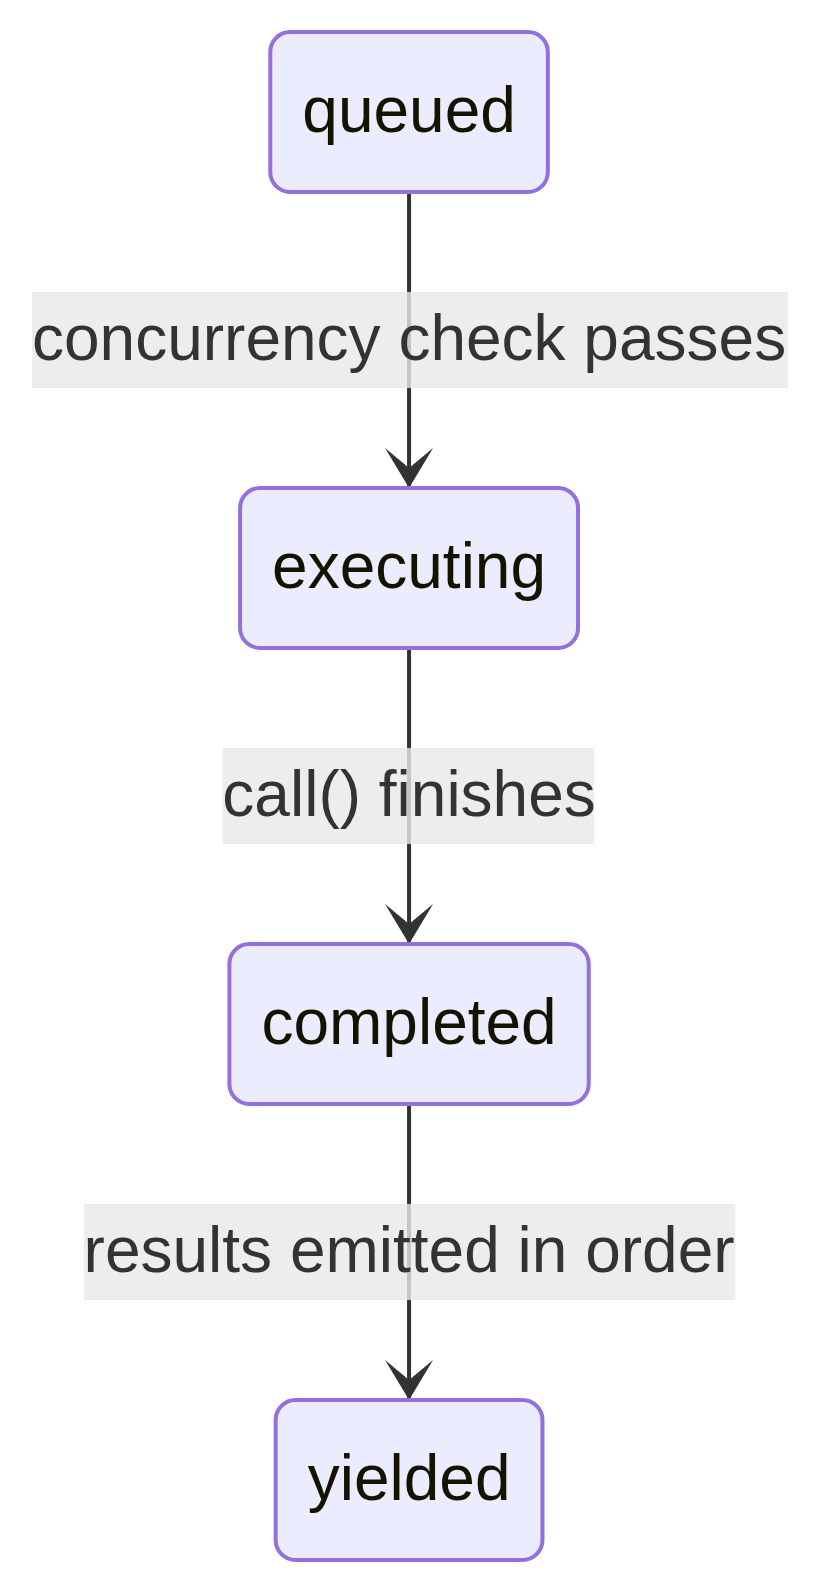
\includegraphics[width=2.13in,height=4.15in]{book/ch07-concurrency_files/figure-latex/mermaid-figure-2.png}

\begin{itemize}
\tightlist
\item
  \textbf{queued}: The \texttt{tool\_use} block has been parsed and
  registered. Waiting for concurrency conditions to allow execution.
\item
  \textbf{executing}: The tool's \texttt{call()} function is running.
  Results accumulate in a buffer.
\item
  \textbf{completed}: Execution finished. Results are ready to be
  yielded to the conversation.
\item
  \textbf{yielded}: Results have been emitted. Terminal state.
\end{itemize}

\subsection{addTool(): Queuing During the
Stream}\label{addtool-queuing-during-the-stream}

\begin{Shaded}
\begin{Highlighting}[]
\FunctionTok{addTool}\NormalTok{(block}\OperatorTok{:}\NormalTok{ ToolUseBlock}\OperatorTok{,}\NormalTok{ assistantMessage}\OperatorTok{:}\NormalTok{ AssistantMessage)}\OperatorTok{:} \DataTypeTok{void}
\end{Highlighting}
\end{Shaded}

Called by the streaming response parser each time a complete
\texttt{tool\_use} block arrives. The method:

\begin{enumerate}
\def\labelenumi{\arabic{enumi}.}
\tightlist
\item
  Looks up the tool definition. If not found, immediately creates a
  \texttt{completed} entry with an error message -- no point in queuing
  a tool that does not exist.
\item
  Parses the input and determines \texttt{isConcurrencySafe} using the
  same logic as \texttt{partitionToolCalls()}.
\item
  Pushes a \texttt{TrackedTool} with status
  \texttt{\textquotesingle{}queued\textquotesingle{}}.
\item
  Calls \texttt{processQueue()} -- which may start the tool immediately.
\end{enumerate}

The call to \texttt{processQueue()} is fire-and-forget
(\texttt{void\ this.processQueue()}). The executor does not await it.
This is intentional: \texttt{addTool()} is called from the streaming
parser's event handler, and blocking there would stall response parsing.
The tool starts executing in the background while the parser continues
consuming the stream.

\subsection{processQueue(): The Admission
Check}\label{processqueue-the-admission-check}

The admission check is a single predicate:

\begin{Shaded}
\begin{Highlighting}[]
\CommentTok{// Pseudocode — illustrates the mutual exclusion rule}
\NormalTok{canRun }\OperatorTok{=}\NormalTok{ noToolsRunning }\OperatorTok{||}\NormalTok{ (newToolIsSafe }\OperatorTok{\&\&}\NormalTok{ allRunningAreSafe)}
\end{Highlighting}
\end{Shaded}

A tool can start executing if and only if: - \textbf{No tools are
currently executing} (the queue is empty), OR - \textbf{Both the new
tool and all currently executing tools are concurrency-safe.}

This is a mutual exclusion contract. A non-concurrent tool requires
exclusive access -- nothing else can be running. Concurrent tools can
share the runway with other concurrent tools, but a single
non-concurrent tool in the executing set blocks everyone.

The \texttt{processQueue()} method iterates through all tools in order.
For each queued tool, it checks \texttt{canExecuteTool()}. If the tool
can run, it starts. If a non-concurrent tool cannot run yet, the loop
\emph{breaks} -- it stops checking subsequent tools entirely, because
non-concurrent tools must maintain ordering. If a concurrent tool cannot
run (blocked by an executing non-concurrent tool), the loop
\emph{continues} -- but in practice this rarely helps, because
concurrent tools after a non-concurrent blocker are typically dependent
on its results anyway.

\subsection{executeTool(): The Core Execution
Loop}\label{executetool-the-core-execution-loop}

This method is where the real complexity lives. It manages abort
controllers, error cascades, progress reporting, and context modifiers.

\textbf{Child abort controllers.} Each tool gets its own
\texttt{AbortController} that is a child of a shared sibling-level
controller.

The hierarchy is three levels deep: the query-level controller (owned by
the REPL, fires on user Ctrl+C) parents the sibling controller (owned by
the streaming executor, fires on Bash errors) which parents each tool's
individual controller. Aborting the sibling controller kills all running
tools. Aborting a tool's individual controller kills only that tool --
but it also bubbles up to the query controller if the abort reason is
not a sibling error. This bubble-up prevents the system from silently
discarding the executor when, for example, a permission denial should
end the entire turn.

This bubble-up is essential for permission denial. When a user rejects a
tool in the permission dialog, the tool's abort controller fires. That
signal must reach the query loop so it can end the turn. Without it, the
query loop would continue as if nothing happened, sending a stale
rejection message to the model.

\textbf{The sibling error cascade.} When a tool produces an error
result, the executor checks whether to cancel sibling tools. The rule:
\textbf{only Bash errors cascade.} When a shell command errors, the
executor records the failure, captures a description of the errored
tool, and aborts the sibling controller -- which cancels all other
running tools in the batch.

The rationale is pragmatic. Bash commands often form implicit dependency
chains:
\texttt{mkdir\ build\ \&\&\ cp\ src/*\ build/\ \&\&\ tar\ -czf\ dist.tar.gz\ build/}.
If \texttt{mkdir} fails, running \texttt{cp} and \texttt{tar} is
pointless. Canceling siblings immediately saves time and avoids
confusing error messages.

Read and Grep errors, by contrast, are independent. If one file read
fails because the file was deleted, that has no bearing on a concurrent
grep searching a different directory. Canceling the grep would waste
work for no reason.

The error cascade produces synthetic error messages for sibling tools:

\begin{verbatim}
Cancelled: parallel tool call Bash(mkdir build) errored
\end{verbatim}

The description includes the first 40 characters of the errored tool's
command or file path, giving the model enough context to understand what
went wrong.

\textbf{Progress messages} are handled separately from results. While
results are buffered and yielded in order, progress messages (status
updates like ``Reading file\ldots{}'' or ``Searching\ldots{}'') go to a
\texttt{pendingProgress} array and are yielded immediately via
\texttt{getCompletedResults()}. A resolve callback wakes up the
\texttt{getRemainingResults()} loop when new progress arrives,
preventing the UI from appearing frozen during long-running tools.

\textbf{Queue re-processing.} After each tool completes,
\texttt{processQueue()} is called again:

\begin{Shaded}
\begin{Highlighting}[]
\KeywordTok{void}\NormalTok{ promise}\OperatorTok{.}\FunctionTok{finally}\NormalTok{(() }\KeywordTok{=\textgreater{}}\NormalTok{ \{}
  \KeywordTok{void} \KeywordTok{this}\OperatorTok{.}\FunctionTok{processQueue}\NormalTok{()}
\NormalTok{\})}
\end{Highlighting}
\end{Shaded}

This is how serial tools that were blocked by a concurrent batch get
started. When the last concurrent tool finishes, the subsequent
non-concurrent tool's \texttt{canExecuteTool()} check passes, and it
begins executing.

\subsection{Result Harvesting}\label{result-harvesting}

The streaming executor exposes two harvesting methods, designed for two
different phases of the response lifecycle.

\textbf{\texttt{getCompletedResults()} -- mid-stream harvesting.} This
is a synchronous generator called between chunks of the streaming API
response. It walks the tools array in order and yields results for any
tools that have completed:

\texttt{getCompletedResults()} is a synchronous generator that walks the
tools array in submission order. For each tool, it first drains any
pending progress messages. If the tool is completed, it yields the
results and marks it as yielded. The critical rule: if a non-concurrent
tool is still executing, the walk \textbf{breaks} -- nothing after it
can be yielded, even if subsequent tools have already completed. Results
after a serial tool might depend on its context modifications, so they
must wait. For concurrent tools, this restriction does not apply; the
loop skips executing concurrent tools and continues checking subsequent
entries.

This break is the order-preservation mechanism. If a non-concurrent tool
is still executing, nothing after it can be yielded -- even if
subsequent tools have already completed. Results after a serial tool
might depend on its context modifications, so they must wait. For
concurrent tools, this restriction does not apply; the loop skips
executing concurrent tools and continues checking subsequent entries.

\textbf{\texttt{getRemainingResults()} -- post-stream drain.} Called
after the model's response is fully received. This async generator loops
until every tool is yielded:

\texttt{getRemainingResults()} is the post-stream drain. It loops until
every tool is yielded. On each iteration, it processes the queue
(starting any newly-unblocked tools), yields any completed results via
\texttt{getCompletedResults()}, and then -- if tools are still executing
but nothing new has completed -- uses \texttt{Promise.race} to idle-wait
on whichever finishes first: any executing tool's promise, or a
progress-available signal. This avoids busy-polling while still waking
up the moment something happens. When no tools have completed and
nothing new can start, the executor waits for any executing tool to
finish (or for progress to arrive). This avoids busy-polling while still
waking up the moment something happens.

\subsection{Order Preservation}\label{order-preservation}

Results are yielded in the order tools were \emph{received}, not the
order they \emph{completed}. This is a deliberate design choice.

Consider a model response that requests
\texttt{{[}Read("a.ts"),\ Read("b.ts"),\ Read("c.ts"){]}}. All three
start concurrently. \texttt{c.ts} finishes first (it is smaller), then
\texttt{a.ts}, then \texttt{b.ts}. If results were yielded in completion
order, the conversation would show:

\begin{verbatim}
Tool result: c.ts contents
Tool result: a.ts contents
Tool result: b.ts contents
\end{verbatim}

But the model emitted them in a-b-c order. The conversation history must
match the model's expectation, or the next turn will be confused about
which result corresponds to which request. By yielding in arrival order,
the conversation stays coherent:

\begin{verbatim}
Tool result: a.ts contents  (completed second, yielded first)
Tool result: b.ts contents  (completed third, yielded second)
Tool result: c.ts contents  (completed first, yielded third)
\end{verbatim}

The cost is minor: if tool 1 is slow and tools 2-5 are fast, the fast
results sit in buffers until tool 1 finishes. But the alternative --
conversation incoherence -- is far worse.

\subsection{discard(): The Streaming Fallback Escape
Hatch}\label{discard-the-streaming-fallback-escape-hatch}

When the API response stream fails mid-way (network error, server
disconnect), the system retries with a new API call. But the streaming
executor may have already started tools from the failed attempt. Those
results are now orphaned -- they correspond to a response that was never
fully received.

\begin{Shaded}
\begin{Highlighting}[]
\FunctionTok{discard}\NormalTok{()}\OperatorTok{:} \DataTypeTok{void}\NormalTok{ \{}
  \KeywordTok{this}\OperatorTok{.}\AttributeTok{discarded} \OperatorTok{=} \KeywordTok{true}
\NormalTok{\}}
\end{Highlighting}
\end{Shaded}

Setting \texttt{discarded\ =\ true} causes: -
\texttt{getCompletedResults()} returns immediately with no results. -
\texttt{getRemainingResults()} returns immediately with no results. -
Any tool that starts executing checks \texttt{getAbortReason()}, sees
\texttt{streaming\_fallback}, and gets a synthetic error instead of
actually running.

The discarded executor is abandoned. A fresh executor is created for the
retry attempt.

\begin{center}\rule{0.5\linewidth}{0.5pt}\end{center}

\section{Tool Concurrency Properties}\label{tool-concurrency-properties}

Each built-in tool declares its concurrency characteristics through the
\texttt{isConcurrencySafe()} method. The classification is not arbitrary
-- it reflects the tool's actual effect on shared state.

\begin{longtable}[]{@{}
  >{\raggedright\arraybackslash}p{(\linewidth - 6\tabcolsep) * \real{0.1333}}
  >{\raggedright\arraybackslash}p{(\linewidth - 6\tabcolsep) * \real{0.3778}}
  >{\raggedright\arraybackslash}p{(\linewidth - 6\tabcolsep) * \real{0.2444}}
  >{\raggedright\arraybackslash}p{(\linewidth - 6\tabcolsep) * \real{0.2444}}@{}}
\toprule\noalign{}
\begin{minipage}[b]{\linewidth}\raggedright
Tool
\end{minipage} & \begin{minipage}[b]{\linewidth}\raggedright
Concurrency Safe
\end{minipage} & \begin{minipage}[b]{\linewidth}\raggedright
Condition
\end{minipage} & \begin{minipage}[b]{\linewidth}\raggedright
Rationale
\end{minipage} \\
\midrule\noalign{}
\endhead
\bottomrule\noalign{}
\endlastfoot
\textbf{Read} & Always & -- & Pure read. No side effects. \\
\textbf{Grep} & Always & -- & Pure read. Wraps ripgrep. \\
\textbf{Glob} & Always & -- & Pure read. File listing. \\
\textbf{Fetch} & Always & -- & HTTP GET. No local side effects. \\
\textbf{WebSearch} & Always & -- & API call to search provider. \\
\textbf{Bash} & Sometimes & Read-only commands only &
\texttt{isReadOnly()} parses the command and classifies subcommands.
\texttt{ls}, \texttt{git\ status}, \texttt{cat}, \texttt{grep} are safe.
\texttt{rm}, \texttt{mkdir}, \texttt{mv} are not. \\
\textbf{Edit} & Never & -- & Modifies files. Two concurrent edits to the
same file corrupt it. \\
\textbf{Write} & Never & -- & Creates or overwrites files. Same
corruption risk. \\
\textbf{NotebookEdit} & Never & -- & Modifies \texttt{.ipynb} files. \\
\end{longtable}

The Bash tool's classification deserves elaboration. It uses
\texttt{splitCommandWithOperators()} to decompose compound commands
(\texttt{\&\&}, \texttt{\textbar{}\textbar{}}, \texttt{;},
\texttt{\textbar{}}), then classifies each subcommand against known-safe
sets:

\begin{itemize}
\tightlist
\item
  \textbf{Search commands}: \texttt{grep}, \texttt{rg}, \texttt{find},
  \texttt{fd}, \texttt{ag}, \texttt{ack}
\item
  \textbf{Read commands}: \texttt{cat}, \texttt{head}, \texttt{tail},
  \texttt{wc}, \texttt{jq}, \texttt{less}, \texttt{file}, \texttt{stat}
\item
  \textbf{List commands}: \texttt{ls}, \texttt{tree}, \texttt{du},
  \texttt{df}
\item
  \textbf{Neutral commands}: \texttt{echo}, \texttt{printf} (no side
  effects but not ``reads'')
\end{itemize}

A compound command is read-only only if every non-neutral subcommand is
in the search, read, or list set. \texttt{ls\ -la\ \&\&\ cat\ README.md}
is safe. \texttt{ls\ -la\ \&\&\ rm\ -rf\ build/} is not -- the
\texttt{rm} contaminates the entire command.

\begin{center}\rule{0.5\linewidth}{0.5pt}\end{center}

\section{The Interrupt Behavior
Contract}\label{the-interrupt-behavior-contract}

While tools are executing, the user can type a new message. What should
happen? The answer depends on the tool.

Each tool declares an \texttt{interruptBehavior()} method that returns
either \texttt{\textquotesingle{}cancel\textquotesingle{}} or
\texttt{\textquotesingle{}block\textquotesingle{}}:

\begin{itemize}
\tightlist
\item
  \textbf{\texttt{\textquotesingle{}cancel\textquotesingle{}}}: Stop the
  tool immediately, discard partial results, and process the new user
  message. Used by tools where partial execution is harmless (reads,
  searches).
\item
  \textbf{\texttt{\textquotesingle{}block\textquotesingle{}}}: Keep the
  tool running to completion. The user's new message waits. Used by
  tools where interruption would leave the system in an inconsistent
  state (writes mid-flight, long-running bash commands). This is the
  default.
\end{itemize}

The streaming executor tracks the interruptible state of the current
tool set:

The interruptible state is updated by checking all currently executing
tools: the set is interruptible only when every executing tool supports
cancellation. If even one tool's interrupt behavior is
\texttt{\textquotesingle{}block\textquotesingle{}}, the entire set is
treated as non-interruptible.

The UI only shows an ``interruptible'' indicator when ALL executing
tools support cancellation. If even one tool is
\texttt{\textquotesingle{}block\textquotesingle{}}, the entire set is
treated as non-interruptible. This is conservative but correct: you
cannot meaningfully interrupt a batch where one tool would keep running
anyway.

When the user does interrupt and all tools are cancellable, the abort
controller fires with reason
\texttt{\textquotesingle{}interrupt\textquotesingle{}}. The executor's
\texttt{getAbortReason()} method checks each tool's interrupt behavior
individually -- a \texttt{\textquotesingle{}cancel\textquotesingle{}}
tool gets a synthetic \texttt{user\_interrupted} error, while a
\texttt{\textquotesingle{}block\textquotesingle{}} tool (which would not
be present in a fully interruptible set, but the code handles the edge
case) continues running.

\begin{center}\rule{0.5\linewidth}{0.5pt}\end{center}

\section{Context Modifiers: The Serial-Only
Contract}\label{context-modifiers-the-serial-only-contract}

Context modifiers are functions of type
\texttt{(context:\ ToolUseContext)\ =\textgreater{}\ ToolUseContext}.
They let a tool say ``I've changed something about the execution
environment that subsequent tools need to know about.''

The contract is simple: \textbf{context modifiers are only applied for
serial (non-concurrent-safe) tools.} This is stated explicitly in the
source:

\begin{Shaded}
\begin{Highlighting}[]
\CommentTok{// }\AlertTok{NOTE}\CommentTok{: we currently don\textquotesingle{}t support context modifiers for concurrent}
\CommentTok{//       tools. None are actively being used, but if we want to use}
\CommentTok{//       them in concurrent tools, we need to support that here.}
\ControlFlowTok{if}\NormalTok{ (}\OperatorTok{!}\NormalTok{tool}\OperatorTok{.}\AttributeTok{isConcurrencySafe} \OperatorTok{\&\&}\NormalTok{ contextModifiers}\OperatorTok{.}\AttributeTok{length} \OperatorTok{\textgreater{}} \DecValTok{0}\NormalTok{) \{}
  \ControlFlowTok{for}\NormalTok{ (}\KeywordTok{const}\NormalTok{ modifier }\KeywordTok{of}\NormalTok{ contextModifiers) \{}
    \KeywordTok{this}\OperatorTok{.}\AttributeTok{toolUseContext} \OperatorTok{=} \FunctionTok{modifier}\NormalTok{(}\KeywordTok{this}\OperatorTok{.}\AttributeTok{toolUseContext}\NormalTok{)}
\NormalTok{  \}}
\NormalTok{\}}
\end{Highlighting}
\end{Shaded}

In the batch orchestration path (\texttt{toolOrchestration.ts}),
concurrent batch modifiers are collected and applied after the batch
completes, in tool-submission order. This means concurrent tools within
a batch cannot see each other's context changes, but the batch after
them can.

The asymmetry is intentional. If Tool A modifies context and Tool B
reads that context, they have a data dependency. Data dependencies mean
they cannot run concurrently. By definition, if two tools are
concurrency-safe, neither should depend on the other's context
modifications. The system enforces this by deferring application.

\begin{center}\rule{0.5\linewidth}{0.5pt}\end{center}

\section{Apply This}\label{apply-this-4}

The concurrency patterns in Claude Code generalize to any system that
orchestrates multiple independent operations. Three principles are worth
extracting.

\textbf{Partition by safety, not by type.} The
\texttt{isConcurrencySafe(input)} method receives the parsed input, not
just the tool name. This per-invocation classification is more precise
than a static ``this tool type is always safe'' declaration. In your own
systems, inspect the operation's arguments before deciding whether to
parallelize. A database read is safe to parallelize; a database write to
the same row is not. The operation type alone does not tell you enough.

\textbf{Speculative execution during I/O waits.} The streaming executor
starts tools while the API response is still arriving. The same pattern
applies anywhere you have a slow producer and fast consumers: start
processing early items while later items are still being generated.
HTTP/2 server push, compiler pipeline parallelism, and speculative CPU
execution all share this structure. The key requirement is that you can
identify independent work before the full instruction set is available.

\textbf{Preserve submission order in results.} Yielding results in
completion order is tempting -- it minimizes latency to first result.
But if the consumer (in this case, the language model) expects results
in a specific order, reordering them creates confusion that costs more
time to resolve than the latency savings. Buffer completed results and
release them in the order they were requested. The implementation cost
is a simple array walk; the correctness benefit is absolute.

The streaming executor pattern is particularly powerful for agent
systems. Any time your agent loop involves a ``think, then act'' cycle
where the thinking phase produces multiple independent actions, you can
overlap the tail of thinking with the beginning of acting. The savings
are proportional to the ratio of think-time to act-time. For language
model agents, where think-time (API response generation) dominates, the
savings are substantial.

\begin{center}\rule{0.5\linewidth}{0.5pt}\end{center}

\section{Summary}\label{summary-1}

Claude Code's concurrency system operates at two levels. The partition
algorithm (\texttt{partitionToolCalls}) groups consecutive
concurrency-safe tools into batches that run in parallel, while
isolating unsafe tools into serial batches where each tool sees the
effects of the one before it. The streaming tool executor
(\texttt{StreamingToolExecutor}) goes further, starting tools
speculatively as they arrive during model response streaming,
overlapping tool execution with response generation.

The safety model is conservative by design. Concurrency safety is
determined per-invocation by inspecting parsed inputs. Unknown tools
default to serial. Parsing failures default to serial. Exceptions in
safety checks default to serial. The system never guesses that something
is safe to parallelize -- the tool must affirmatively declare it.

Error handling follows the dependency structure of the tools. Bash
errors cascade to siblings because shell commands often form implicit
pipelines. Read and search errors are isolated because they are
independent operations. The abort controller hierarchy -- query
controller, sibling controller, per-tool controller -- gives each level
the ability to cancel its scope without disrupting the level above.

The result is a system that extracts maximum parallelism from the
model's tool requests while maintaining the invariant that the
conversation history reflects a coherent, ordered sequence of actions.
The model sees results in the order it requested them. The user sees
tools complete as fast as the underlying operations allow. The gap
between those two -- execution speed vs.~presentation order -- is
bridged by buffering, and that buffer is the simplest part of the entire
system.

\part{Part III: Multi-Agent Orchestration}

\chapter{Chapter 8: Spawning
Sub-Agents}\label{chapter-8-spawning-sub-agents}

\section{The Multiplication of
Intelligence}\label{the-multiplication-of-intelligence}

A single agent is powerful. It can read files, edit code, run tests,
search the web, and reason about the results. But there is a hard
ceiling on what one agent can do in a single conversation: the context
window fills up, the task branches in directions that demand different
capabilities, and the serial nature of tool execution becomes a
bottleneck. The solution is not a bigger model. It is more agents.

Claude Code's sub-agent system lets the model request help. When the
parent agent encounters a task that would benefit from delegation -- a
codebase search that should not pollute the main conversation, a
verification pass that demands adversarial thinking, a set of
independent edits that could run in parallel -- it calls the
\texttt{Agent} tool. That call spawns a child: a fully independent agent
with its own conversation loop, its own tool set, its own permission
boundary, and its own abort controller. The child does its work and
returns a result. The parent never sees the child's internal reasoning,
only the final output.

This is not a convenience feature. It is the architectural foundation
for everything from parallel file exploration to coordinator-worker
hierarchies to multi-agent swarm teams. And it all flows through two
files: \texttt{AgentTool.tsx}, which defines the model-facing interface,
and \texttt{runAgent.ts}, which implements the lifecycle.

The design challenge is significant. A sub-agent needs enough context to
do its job but not so much that it wastes tokens on irrelevant
information. It needs permission boundaries that are strict enough for
safety but flexible enough for utility. It needs lifecycle management
that cleans up every resource it touches without requiring the caller to
remember what to clean up. And all of this must work for a spectrum of
agent types -- from a cheap, fast, read-only Haiku searcher to an
expensive, thorough, Opus-powered verification agent running adversarial
tests in the background.

This chapter traces the path from the model's ``I need help'' to a fully
operational child agent. We will examine the tool definition that the
model sees, the fifteen-step lifecycle that creates the execution
environment, the six built-in agent types and what each optimizes for,
the frontmatter system that lets users define custom agents, and the
design principles that emerge from all of it.

A note on terminology: throughout this chapter, ``parent'' refers to the
agent that calls the \texttt{Agent} tool, and ``child'' refers to the
agent that is spawned. The parent is usually (but not always) the
top-level REPL agent. In coordinator mode, the coordinator spawns
workers, which are children. In nested scenarios, a child can itself
spawn grandchildren -- the same lifecycle applies recursively.

The orchestration layer spans approximately 40 files across
\texttt{tools/AgentTool/}, \texttt{tasks/}, \texttt{coordinator/},
\texttt{tools/SendMessageTool/}, and \texttt{utils/swarm/}. This chapter
focuses on the spawning mechanics -- the AgentTool definition and the
runAgent lifecycle. The next chapter covers the runtime: progress
tracking, result retrieval, and multi-agent coordination patterns.

\begin{center}\rule{0.5\linewidth}{0.5pt}\end{center}

\section{The AgentTool Definition}\label{the-agenttool-definition}

The \texttt{AgentTool} is registered under the name \texttt{"Agent"}
with a legacy alias \texttt{"Task"} for backward compatibility with
older transcripts, permission rules, and hook configurations. It is
built with the standard \texttt{buildTool()} factory, but its schema is
more dynamic than any other tool in the system.

\subsection{The Input Schema}\label{the-input-schema}

The input schema is constructed lazily via \texttt{lazySchema()} -- a
pattern we saw in Chapter 6 that defers zod compilation until first use.
There are two layers: a base schema and a full schema that adds
multi-agent and isolation parameters.

The base fields are always present:

\begin{longtable}[]{@{}
  >{\raggedright\arraybackslash}p{(\linewidth - 6\tabcolsep) * \real{0.2188}}
  >{\raggedright\arraybackslash}p{(\linewidth - 6\tabcolsep) * \real{0.1875}}
  >{\raggedright\arraybackslash}p{(\linewidth - 6\tabcolsep) * \real{0.3125}}
  >{\raggedright\arraybackslash}p{(\linewidth - 6\tabcolsep) * \real{0.2812}}@{}}
\toprule\noalign{}
\begin{minipage}[b]{\linewidth}\raggedright
Field
\end{minipage} & \begin{minipage}[b]{\linewidth}\raggedright
Type
\end{minipage} & \begin{minipage}[b]{\linewidth}\raggedright
Required
\end{minipage} & \begin{minipage}[b]{\linewidth}\raggedright
Purpose
\end{minipage} \\
\midrule\noalign{}
\endhead
\bottomrule\noalign{}
\endlastfoot
\texttt{description} & \texttt{string} & Yes & Short 3-5 word summary of
the task \\
\texttt{prompt} & \texttt{string} & Yes & The full task description for
the agent \\
\texttt{subagent\_type} & \texttt{string} & No & Which specialized agent
to use \\
\texttt{model} &
\texttt{enum(\textquotesingle{}sonnet\textquotesingle{},\textquotesingle{}opus\textquotesingle{},\textquotesingle{}haiku\textquotesingle{})}
& No & Model override for this agent \\
\texttt{run\_in\_background} & \texttt{boolean} & No & Launch
asynchronously \\
\end{longtable}

The full schema adds multi-agent parameters (when swarm features are
active) and isolation controls:

\begin{longtable}[]{@{}
  >{\raggedright\arraybackslash}p{(\linewidth - 4\tabcolsep) * \real{0.3182}}
  >{\raggedright\arraybackslash}p{(\linewidth - 4\tabcolsep) * \real{0.2727}}
  >{\raggedright\arraybackslash}p{(\linewidth - 4\tabcolsep) * \real{0.4091}}@{}}
\toprule\noalign{}
\begin{minipage}[b]{\linewidth}\raggedright
Field
\end{minipage} & \begin{minipage}[b]{\linewidth}\raggedright
Type
\end{minipage} & \begin{minipage}[b]{\linewidth}\raggedright
Purpose
\end{minipage} \\
\midrule\noalign{}
\endhead
\bottomrule\noalign{}
\endlastfoot
\texttt{name} & \texttt{string} & Makes the agent addressable via
\texttt{SendMessage(\{to:\ name\})} \\
\texttt{team\_name} & \texttt{string} & Team context for spawning \\
\texttt{mode} & \texttt{PermissionMode} & Permission mode for spawned
teammate \\
\texttt{isolation} &
\texttt{enum(\textquotesingle{}worktree\textquotesingle{},\textquotesingle{}remote\textquotesingle{})}
& Filesystem isolation strategy \\
\texttt{cwd} & \texttt{string} & Absolute path override for working
directory \\
\end{longtable}

The multi-agent fields enable the swarm pattern covered in Chapter 9:
named agents that can send messages to each other via
\texttt{SendMessage(\{to:\ name\})} while running concurrently. The
isolation fields enable filesystem safety: worktree isolation creates a
temporary git worktree so the agent operates on a copy of the
repository, preventing conflicting edits when multiple agents work on
the same codebase simultaneously.

What makes this schema unusual is that it is \textbf{dynamically shaped
by feature flags}:

\begin{Shaded}
\begin{Highlighting}[]
\CommentTok{// Pseudocode — illustrates the feature{-}gated schema pattern}
\NormalTok{inputSchema }\OperatorTok{=} \FunctionTok{lazySchema}\NormalTok{(() }\KeywordTok{=\textgreater{}}\NormalTok{ \{}
  \KeywordTok{let}\NormalTok{ schema }\OperatorTok{=} \FunctionTok{baseSchema}\NormalTok{()}
  \ControlFlowTok{if}\NormalTok{ (}\OperatorTok{!}\FunctionTok{featureEnabled}\NormalTok{(}\StringTok{\textquotesingle{}ASSISTANT\_MODE\textquotesingle{}}\NormalTok{)) schema }\OperatorTok{=}\NormalTok{ schema}\OperatorTok{.}\FunctionTok{omit}\NormalTok{(\{ cwd}\OperatorTok{:} \KeywordTok{true}\NormalTok{ \})}
  \ControlFlowTok{if}\NormalTok{ (backgroundDisabled }\OperatorTok{||}\NormalTok{ forkMode)    schema }\OperatorTok{=}\NormalTok{ schema}\OperatorTok{.}\FunctionTok{omit}\NormalTok{(\{ run\_in\_background}\OperatorTok{:} \KeywordTok{true}\NormalTok{ \})}
  \ControlFlowTok{return}\NormalTok{ schema}
\NormalTok{\})}
\end{Highlighting}
\end{Shaded}

When the fork experiment is active, \texttt{run\_in\_background}
disappears from the schema entirely because all spawns are forced async
under that path. When background tasks are disabled (via
\texttt{CLAUDE\_CODE\_DISABLE\_BACKGROUND\_TASKS}), the field is also
stripped. When the KAIROS feature flag is off, \texttt{cwd} is omitted.
The model never sees fields it cannot use.

This is a subtle but important design choice. The schema is not just
validation -- it is the model's instruction manual. Every field in the
schema is described in the tool definition that the model reads.
Removing fields the model should not use is more effective than adding
``do not use this field'' to the prompt. The model cannot misuse what it
cannot see.

\subsection{The Output Schema}\label{the-output-schema}

The output is a discriminated union with two public variants:

\begin{itemize}
\tightlist
\item
  \texttt{\{\ status:\ \textquotesingle{}completed\textquotesingle{},\ prompt,\ ...AgentToolResult\ \}}
  -- synchronous completion with the agent's final output
\item
  \texttt{\{\ status:\ \textquotesingle{}async\_launched\textquotesingle{},\ agentId,\ description,\ prompt,\ outputFile\ \}}
  -- background launch acknowledgment
\end{itemize}

Two additional internal variants (\texttt{TeammateSpawnedOutput} and
\texttt{RemoteLaunchedOutput}) exist but are excluded from the exported
schema to enable dead code elimination in external builds. The bundler
strips these variants and their associated code paths when the
corresponding feature flags are disabled, keeping the distributed binary
smaller.

The \texttt{async\_launched} variant is notable for what it includes:
the \texttt{outputFile} path where the agent's results will be written
when it completes. This lets the parent (or any other consumer) poll or
watch the file for results, providing a filesystem-based communication
channel that survives process restarts.

\subsection{The Dynamic Prompt}\label{the-dynamic-prompt}

The \texttt{AgentTool} prompt is generated by \texttt{getPrompt()} and
is context-sensitive. It adapts based on available agents (listed inline
or as an attachment to avoid busting prompt cache), whether fork is
active (adds ``When to fork'' guidance), whether the session is in
coordinator mode (slim prompt since the coordinator system prompt
already covers usage), and subscription tier. Non-pro users get a note
about launching multiple agents concurrently.

The attachment-based agent list is worth highlighting. The codebase
comments reference ``approximately 10.2\% of fleet cache\_creation
tokens'' being caused by dynamic tool descriptions. Moving the agent
list from the tool description to an attachment message keeps the tool
description static, so connecting an MCP server or loading a plugin does
not bust the prompt cache for every subsequent API call.

This is a pattern worth internalizing for any system that uses tool
definitions with dynamic content. The Anthropic API caches the prompt
prefix -- system prompt, tool definitions, and conversation history --
and reuses the cached computation for subsequent requests that share the
same prefix. If the tool definition changes between API calls (because
an agent was added or an MCP server connected), the entire cache is
invalidated. Moving volatile content from the tool definition (which is
part of the cached prefix) to an attachment message (which is appended
after the cached portion) preserves the cache while still delivering the
information to the model.

With the tool definition understood, we can now trace what happens when
the model actually calls it.

\subsection{Feature Gating}\label{feature-gating}

The sub-agent system has the most complex feature gating in the
codebase. At least twelve feature flags and GrowthBook experiments
control which agents are available, which parameters appear in the
schema, and which code paths are taken:

\begin{longtable}[]{@{}
  >{\raggedright\arraybackslash}p{(\linewidth - 2\tabcolsep) * \real{0.5652}}
  >{\raggedright\arraybackslash}p{(\linewidth - 2\tabcolsep) * \real{0.4348}}@{}}
\toprule\noalign{}
\begin{minipage}[b]{\linewidth}\raggedright
Feature Gate
\end{minipage} & \begin{minipage}[b]{\linewidth}\raggedright
Controls
\end{minipage} \\
\midrule\noalign{}
\endhead
\bottomrule\noalign{}
\endlastfoot
\texttt{FORK\_SUBAGENT} & Fork agent path \\
\texttt{BUILTIN\_EXPLORE\_PLAN\_AGENTS} & Explore and Plan agents \\
\texttt{VERIFICATION\_AGENT} & Verification agent \\
\texttt{KAIROS} & \texttt{cwd} override, assistant force-async \\
\texttt{TRANSCRIPT\_CLASSIFIER} & Handoff classification, \texttt{auto}
mode override \\
\texttt{PROACTIVE} & Proactive module integration \\
\end{longtable}

Each gate uses \texttt{feature()} from Bun's dead code elimination
system (compile-time) or
\texttt{getFeatureValue\_CACHED\_MAY\_BE\_STALE()} from GrowthBook
(runtime A/B testing). The compile-time gates are string-replaced during
the build -- when \texttt{FORK\_SUBAGENT} is
\texttt{\textquotesingle{}ant\textquotesingle{}}, the entire fork code
path is included; when it is
\texttt{\textquotesingle{}external\textquotesingle{}}, it may be
excluded entirely. The GrowthBook gates allow live experimentation: the
\texttt{tengu\_amber\_stoat} experiment can A/B test whether removing
Explore and Plan agents changes user behavior, without shipping a new
binary.

\subsection{The call() Decision Tree}\label{the-call-decision-tree}

Before \texttt{runAgent()} is ever invoked, the \texttt{call()} method
in \texttt{AgentTool.tsx} routes the request through a decision tree
that determines \emph{what kind} of agent to spawn and \emph{how} to
spawn it:

\begin{verbatim}
1. Is this a teammate spawn? (team_name + name both set)
   YES -> spawnTeammate() -> return teammate_spawned
   NO  -> continue

2. Resolve effective agent type
   - subagent_type provided -> use it
   - subagent_type omitted, fork enabled -> undefined (fork path)
   - subagent_type omitted, fork disabled -> "general-purpose" (default)

3. Is this the fork path? (effectiveType === undefined)
   YES -> Recursive fork guard check -> Use FORK_AGENT definition

4. Resolve agent definition from activeAgents list
   - Filter by permission deny rules
   - Filter by allowedAgentTypes
   - Throw if not found or denied

5. Check required MCP servers (wait up to 30s for pending)

6. Resolve isolation mode (param overrides agent def)
   - "remote" -> teleportToRemote() -> return remote_launched
   - "worktree" -> createAgentWorktree()
   - null -> normal execution

7. Determine sync vs async
   shouldRunAsync = run_in_background || selectedAgent.background ||
                    isCoordinator || forceAsync || isProactiveActive

8. Assemble worker tool pool

9. Build system prompt and prompt messages

10. Execute (async -> registerAsyncAgent + void lifecycle; sync -> iterate runAgent)
\end{verbatim}

Steps 1 through 6 are pure routing -- no agent has been created yet. The
actual lifecycle begins at \texttt{runAgent()}, which the sync path
iterates directly and the async path wraps in
\texttt{runAsyncAgentLifecycle()}.

The routing is done in \texttt{call()} rather than \texttt{runAgent()}
for a reason: \texttt{runAgent()} is a pure lifecycle function that does
not know about teammates, remote agents, or the fork experiment. It
receives a resolved agent definition and executes it. The decision of
\emph{which} definition to resolve, \emph{how} to isolate the agent, and
\emph{whether} to run synchronously or asynchronously belongs to the
layer above. This separation keeps \texttt{runAgent()} testable and
reusable -- it is called from both the normal AgentTool path and from
the async lifecycle wrapper when resuming a backgrounded agent.

The fork guard in step 3 deserves attention. Fork children keep the
\texttt{Agent} tool in their pool (for cache-identical tool definitions
with the parent), but recursive forking would be pathological. Two
guards prevent it:
\texttt{querySource\ ===\ \textquotesingle{}agent:builtin:fork\textquotesingle{}}
(set on the child's context options, survives autocompact) and
\texttt{isInForkChild(messages)} (scans conversation history for the
\texttt{\textless{}fork-boilerplate\textgreater{}} tag as a fallback).
Belt and suspenders -- the primary guard is fast and reliable; the
fallback catches edge cases where querySource was not threaded.

\begin{center}\rule{0.5\linewidth}{0.5pt}\end{center}

\section{The runAgent Lifecycle}\label{the-runagent-lifecycle}

\texttt{runAgent()} in \texttt{runAgent.ts} is an async generator that
drives a sub-agent's entire lifecycle. It yields \texttt{Message}
objects as the agent works. Every sub-agent -- fork, built-in, custom,
coordinator worker -- flows through this single function. The function
is approximately 400 lines, and every line exists for a reason.

The function signature reveals the complexity of the problem:

\begin{Shaded}
\begin{Highlighting}[]
\ImportTok{export} \KeywordTok{async} \KeywordTok{function}\OperatorTok{*} \FunctionTok{runAgent}\NormalTok{(\{}
\NormalTok{  agentDefinition}\OperatorTok{,}       \CommentTok{// What kind of agent}
\NormalTok{  promptMessages}\OperatorTok{,}        \CommentTok{// What to tell it}
\NormalTok{  toolUseContext}\OperatorTok{,}        \CommentTok{// Parent\textquotesingle{}s execution context}
\NormalTok{  canUseTool}\OperatorTok{,}           \CommentTok{// Permission callback}
\NormalTok{  isAsync}\OperatorTok{,}              \CommentTok{// Background or blocking?}
\NormalTok{  canShowPermissionPrompts}\OperatorTok{,}
\NormalTok{  forkContextMessages}\OperatorTok{,}  \CommentTok{// Parent\textquotesingle{}s history (fork only)}
\NormalTok{  querySource}\OperatorTok{,}          \CommentTok{// Origin tracking}
\NormalTok{  override}\OperatorTok{,}             \CommentTok{// System prompt, abort controller, agent ID overrides}
\NormalTok{  model}\OperatorTok{,}                \CommentTok{// Model override from caller}
\NormalTok{  maxTurns}\OperatorTok{,}             \CommentTok{// Turn limit}
\NormalTok{  availableTools}\OperatorTok{,}       \CommentTok{// Pre{-}assembled tool pool}
\NormalTok{  allowedTools}\OperatorTok{,}         \CommentTok{// Permission scoping}
\NormalTok{  onCacheSafeParams}\OperatorTok{,}    \CommentTok{// Callback for background summarization}
\NormalTok{  useExactTools}\OperatorTok{,}        \CommentTok{// Fork path: use parent\textquotesingle{}s exact tools}
\NormalTok{  worktreePath}\OperatorTok{,}         \CommentTok{// Isolation directory}
\NormalTok{  description}\OperatorTok{,}          \CommentTok{// Human{-}readable task description}
  \CommentTok{// ...}
\NormalTok{\}}\OperatorTok{:}\NormalTok{ \{ }\OperatorTok{...}\NormalTok{ \})}\OperatorTok{:}\NormalTok{ AsyncGenerator}\OperatorTok{\textless{}}\NormalTok{Message}\OperatorTok{,} \DataTypeTok{void}\OperatorTok{\textgreater{}}
\end{Highlighting}
\end{Shaded}

Seventeen parameters. Each one represents a dimension of variation that
the lifecycle must handle. This is not over-engineering -- it is the
natural consequence of a single function serving fork agents, built-in
agents, custom agents, sync agents, async agents, worktree-isolated
agents, and coordinator workers. The alternative would be seven
different lifecycle functions with duplicated logic, which is worse.

The \texttt{override} object is particularly important -- it is the
escape hatch for fork agents and resumed agents that need to inject
pre-computed values (system prompt, abort controller, agent ID) into the
lifecycle without re-deriving them.

Here are the fifteen steps.

\subsection{Step 1: Model Resolution}\label{step-1-model-resolution}

\begin{Shaded}
\begin{Highlighting}[]
\KeywordTok{const}\NormalTok{ resolvedAgentModel }\OperatorTok{=} \FunctionTok{getAgentModel}\NormalTok{(}
\NormalTok{  agentDefinition}\OperatorTok{.}\AttributeTok{model}\OperatorTok{,}                    \CommentTok{// Agent\textquotesingle{}s declared preference}
\NormalTok{  toolUseContext}\OperatorTok{.}\AttributeTok{options}\OperatorTok{.}\AttributeTok{mainLoopModel}\OperatorTok{,}      \CommentTok{// Parent\textquotesingle{}s model}
\NormalTok{  model}\OperatorTok{,}                                    \CommentTok{// Caller\textquotesingle{}s override (from input)}
\NormalTok{  permissionMode}\OperatorTok{,}                           \CommentTok{// Current permission mode}
\NormalTok{)}
\end{Highlighting}
\end{Shaded}

The resolution chain is: \textbf{caller override \textgreater{} agent
definition \textgreater{} parent model \textgreater{} default}. The
\texttt{getAgentModel()} function handles special values like
\texttt{\textquotesingle{}inherit\textquotesingle{}} (use whatever the
parent uses) and GrowthBook-gated overrides for specific agent types.
The Explore agent, for example, defaults to Haiku for external users --
the cheapest and fastest model, appropriate for a read-only search
specialist that runs 34 million times per week.

Why this order matters: the caller (the parent model) can override the
agent definition's preference by passing a \texttt{model} parameter in
the tool call. This lets the parent promote a normally-cheap agent to a
more capable model for a particularly complex search, or demote an
expensive agent when the task is simple. But the agent definition's
model is the default, not the parent's -- a Haiku Explore agent should
not accidentally inherit the parent's Opus model just because no one
specified otherwise.

Understanding the model resolution chain is important because it
establishes a design principle that recurs throughout the lifecycle:
\textbf{explicit overrides beat declarations, declarations beat
inheritance, inheritance beats defaults.} This same principle governs
permission modes, abort controllers, and system prompts. The consistency
makes the system predictable -- once you understand one resolution
chain, you understand them all.

\subsection{Step 2: Agent ID Creation}\label{step-2-agent-id-creation}

\begin{Shaded}
\begin{Highlighting}[]
\KeywordTok{const}\NormalTok{ agentId }\OperatorTok{=}\NormalTok{ override}\OperatorTok{?.}\AttributeTok{agentId} \OperatorTok{?}\NormalTok{ override}\OperatorTok{.}\AttributeTok{agentId} \OperatorTok{:} \FunctionTok{createAgentId}\NormalTok{()}
\end{Highlighting}
\end{Shaded}

Agent IDs follow the pattern \texttt{agent-\textless{}hex\textgreater{}}
where the hex part is derived from \texttt{crypto.randomUUID()}. The
branded type \texttt{AgentId} prevents accidental string confusion at
the type level. The override path exists for resumed agents that need to
keep their original ID for transcript continuity.

\subsection{Step 3: Context
Preparation}\label{step-3-context-preparation}

Fork agents and fresh agents diverge here:

\begin{Shaded}
\begin{Highlighting}[]
\KeywordTok{const}\NormalTok{ contextMessages}\OperatorTok{:}\NormalTok{ Message[] }\OperatorTok{=}\NormalTok{ forkContextMessages}
  \OperatorTok{?} \FunctionTok{filterIncompleteToolCalls}\NormalTok{(forkContextMessages)}
  \OperatorTok{:}\NormalTok{ []}
\KeywordTok{const}\NormalTok{ initialMessages}\OperatorTok{:}\NormalTok{ Message[] }\OperatorTok{=}\NormalTok{ [}\OperatorTok{...}\NormalTok{contextMessages}\OperatorTok{,} \OperatorTok{...}\NormalTok{promptMessages]}

\KeywordTok{const}\NormalTok{ agentReadFileState }\OperatorTok{=}\NormalTok{ forkContextMessages }\OperatorTok{!==} \KeywordTok{undefined}
  \OperatorTok{?} \FunctionTok{cloneFileStateCache}\NormalTok{(toolUseContext}\OperatorTok{.}\AttributeTok{readFileState}\NormalTok{)}
  \OperatorTok{:} \FunctionTok{createFileStateCacheWithSizeLimit}\NormalTok{(READ\_FILE\_STATE\_CACHE\_SIZE)}
\end{Highlighting}
\end{Shaded}

For fork agents, the parent's entire conversation history is cloned into
\texttt{contextMessages}. But there is a critical filter:
\texttt{filterIncompleteToolCalls()} strips any \texttt{tool\_use}
blocks that lack matching \texttt{tool\_result} blocks. Without this
filter, the API would reject the malformed conversation. This happens
when the parent is mid-tool-execution at the moment of forking -- the
tool\_use has been emitted but the result has not arrived yet.

The file state cache follows the same fork-or-fresh pattern. Fork
children get a clone of the parent's cache (they already ``know'' which
files have been read). Fresh agents start empty. The clone is a shallow
copy -- file content strings are shared via reference, not duplicated.
This matters for memory: a fork child with a 50-file cache does not
duplicate 50 file contents, it duplicates 50 pointers. The LRU eviction
behavior is independent -- each cache evicts based on its own access
pattern.

\subsection{Step 4: CLAUDE.md
Stripping}\label{step-4-claude.md-stripping}

Read-only agents like Explore and Plan have \texttt{omitClaudeMd:\ true}
in their definitions:

\begin{Shaded}
\begin{Highlighting}[]
\KeywordTok{const}\NormalTok{ shouldOmitClaudeMd }\OperatorTok{=}
\NormalTok{  agentDefinition}\OperatorTok{.}\AttributeTok{omitClaudeMd} \OperatorTok{\&\&}
  \OperatorTok{!}\NormalTok{override}\OperatorTok{?.}\AttributeTok{userContext} \OperatorTok{\&\&}
  \FunctionTok{getFeatureValue\_CACHED\_MAY\_BE\_STALE}\NormalTok{(}\StringTok{\textquotesingle{}tengu\_slim\_subagent\_claudemd\textquotesingle{}}\OperatorTok{,} \KeywordTok{true}\NormalTok{)}
\KeywordTok{const}\NormalTok{ \{ claudeMd}\OperatorTok{:}\NormalTok{ \_omittedClaudeMd}\OperatorTok{,} \OperatorTok{...}\NormalTok{userContextNoClaudeMd \} }\OperatorTok{=}\NormalTok{ baseUserContext}
\KeywordTok{const}\NormalTok{ resolvedUserContext }\OperatorTok{=}\NormalTok{ shouldOmitClaudeMd}
  \OperatorTok{?}\NormalTok{ userContextNoClaudeMd}
  \OperatorTok{:}\NormalTok{ baseUserContext}
\end{Highlighting}
\end{Shaded}

CLAUDE.md files contain project-specific instructions about commit
messages, PR conventions, lint rules, and coding standards. A read-only
search agent does not need any of this -- it cannot commit, cannot
create PRs, cannot edit files. The parent agent has full context and
will interpret the search results. Dropping CLAUDE.md here saves
billions of tokens per week across the fleet -- an aggregate cost
reduction that justifies the added complexity of conditional context
injection.

Similarly, Explore and Plan agents have \texttt{gitStatus} stripped from
system context. The git status snapshot taken at session start can be up
to 40KB and is explicitly labeled as stale. If these agents need git
information, they can run \texttt{git\ status} themselves and get fresh
data.

These are not premature optimizations. At 34 million Explore spawns per
week, every unnecessary token compounds into measurable cost. The
kill-switch (\texttt{tengu\_slim\_subagent\_claudemd}) defaults to true
but can be flipped via GrowthBook if the stripping causes regressions.

\subsection{Step 5: Permission
Isolation}\label{step-5-permission-isolation}

This is the most intricate step. Each agent gets a custom
\texttt{getAppState()} wrapper that overlays its permission
configuration onto the parent's state:

\begin{Shaded}
\begin{Highlighting}[]
\KeywordTok{const}\NormalTok{ agentGetAppState }\OperatorTok{=}\NormalTok{ () }\KeywordTok{=\textgreater{}}\NormalTok{ \{}
  \KeywordTok{const}\NormalTok{ state }\OperatorTok{=}\NormalTok{ toolUseContext}\OperatorTok{.}\FunctionTok{getAppState}\NormalTok{()}
  \KeywordTok{let}\NormalTok{ toolPermissionContext }\OperatorTok{=}\NormalTok{ state}\OperatorTok{.}\AttributeTok{toolPermissionContext}

  \CommentTok{// Override mode unless parent is in bypassPermissions, acceptEdits, or auto}
  \ControlFlowTok{if}\NormalTok{ (agentPermissionMode }\OperatorTok{\&\&}\NormalTok{ canOverride) \{}
\NormalTok{    toolPermissionContext }\OperatorTok{=}\NormalTok{ \{}
      \OperatorTok{...}\NormalTok{toolPermissionContext}\OperatorTok{,}
\NormalTok{      mode}\OperatorTok{:}\NormalTok{ agentPermissionMode}\OperatorTok{,}
\NormalTok{    \}}
\NormalTok{  \}}

  \CommentTok{// Auto{-}deny prompts for agents that can\textquotesingle{}t show UI}
  \KeywordTok{const}\NormalTok{ shouldAvoidPrompts }\OperatorTok{=}
\NormalTok{    canShowPermissionPrompts }\OperatorTok{!==} \KeywordTok{undefined}
      \OperatorTok{?} \OperatorTok{!}\NormalTok{canShowPermissionPrompts}
      \OperatorTok{:}\NormalTok{ agentPermissionMode }\OperatorTok{===} \StringTok{\textquotesingle{}bubble\textquotesingle{}}
        \OperatorTok{?} \KeywordTok{false}
        \OperatorTok{:}\NormalTok{ isAsync}
  \ControlFlowTok{if}\NormalTok{ (shouldAvoidPrompts) \{}
\NormalTok{    toolPermissionContext }\OperatorTok{=}\NormalTok{ \{}
      \OperatorTok{...}\NormalTok{toolPermissionContext}\OperatorTok{,}
\NormalTok{      shouldAvoidPermissionPrompts}\OperatorTok{:} \KeywordTok{true}\OperatorTok{,}
\NormalTok{    \}}
\NormalTok{  \}}

  \CommentTok{// Scope tool allow rules}
  \ControlFlowTok{if}\NormalTok{ (allowedTools }\OperatorTok{!==} \KeywordTok{undefined}\NormalTok{) \{}
\NormalTok{    toolPermissionContext }\OperatorTok{=}\NormalTok{ \{}
      \OperatorTok{...}\NormalTok{toolPermissionContext}\OperatorTok{,}
\NormalTok{      alwaysAllowRules}\OperatorTok{:}\NormalTok{ \{}
\NormalTok{        cliArg}\OperatorTok{:}\NormalTok{ state}\OperatorTok{.}\AttributeTok{toolPermissionContext}\OperatorTok{.}\AttributeTok{alwaysAllowRules}\OperatorTok{.}\AttributeTok{cliArg}\OperatorTok{,}
\NormalTok{        session}\OperatorTok{:}\NormalTok{ [}\OperatorTok{...}\NormalTok{allowedTools]}\OperatorTok{,}
\NormalTok{      \}}\OperatorTok{,}
\NormalTok{    \}}
\NormalTok{  \}}

  \ControlFlowTok{return}\NormalTok{ \{ }\OperatorTok{...}\NormalTok{state}\OperatorTok{,}\NormalTok{ toolPermissionContext}\OperatorTok{,}\NormalTok{ effortValue \}}
\NormalTok{\}}
\end{Highlighting}
\end{Shaded}

There are four distinct concerns layered together:

\textbf{Permission mode cascade.} If the parent is in
\texttt{bypassPermissions}, \texttt{acceptEdits}, or \texttt{auto} mode,
the parent's mode always wins -- the agent definition cannot weaken it.
Otherwise, the agent definition's \texttt{permissionMode} is applied.
This prevents a custom agent from downgrading security when the user has
explicitly set a permissive mode for the session.

\textbf{Prompt avoidance.} Background agents cannot show permission
dialogs -- there is no terminal attached. So
\texttt{shouldAvoidPermissionPrompts} is set to \texttt{true}, which
causes the permission system to auto-deny rather than block. The
exception is \texttt{bubble} mode: these agents surface prompts to the
parent's terminal, so they can always show prompts regardless of
sync/async status.

\textbf{Automated check ordering.} Background agents that \emph{can}
show prompts (bubble mode) set
\texttt{awaitAutomatedChecksBeforeDialog}. This means the classifier and
permission hooks run first; the user is only interrupted if automated
resolution fails. For background work, waiting an extra second for the
classifier is fine -- the user should not be interrupted unnecessarily.

\textbf{Tool permission scoping.} When \texttt{allowedTools} is
provided, it replaces the session-level allow rules entirely. This
prevents parent approvals from leaking through to scoped agents. But
SDK-level permissions (from \texttt{-\/-allowedTools} CLI flag) are
preserved -- those represent the embedding application's explicit
security policy and should apply everywhere.

\subsection{Step 6: Tool Resolution}\label{step-6-tool-resolution}

\begin{Shaded}
\begin{Highlighting}[]
\KeywordTok{const}\NormalTok{ resolvedTools }\OperatorTok{=}\NormalTok{ useExactTools}
  \OperatorTok{?}\NormalTok{ availableTools}
  \OperatorTok{:} \FunctionTok{resolveAgentTools}\NormalTok{(agentDefinition}\OperatorTok{,}\NormalTok{ availableTools}\OperatorTok{,}\NormalTok{ isAsync)}\OperatorTok{.}\AttributeTok{resolvedTools}
\end{Highlighting}
\end{Shaded}

Fork agents use \texttt{useExactTools:\ true}, which passes the parent's
tool array through unchanged. This is not just convenience -- it is a
cache optimization. Different tool definitions serialize differently
(different permission modes produce different tool metadata), and any
divergence in the tool block busts the prompt cache. Fork children need
byte-identical prefixes.

For normal agents, \texttt{resolveAgentTools()} applies a layered
filter: - \texttt{tools:\ {[}\textquotesingle{}*\textquotesingle{}{]}}
means all tools;
\texttt{tools:\ {[}\textquotesingle{}Read\textquotesingle{},\ \textquotesingle{}Bash\textquotesingle{}{]}}
means only those -
\texttt{disallowedTools:\ {[}\textquotesingle{}Agent\textquotesingle{},\ \textquotesingle{}FileEdit\textquotesingle{}{]}}
removes those from the pool - Built-in agents and custom agents have
different base disallowed tool sets - Async agents get filtered through
\texttt{ASYNC\_AGENT\_ALLOWED\_TOOLS}

The result is that each agent type sees exactly the tools it should
have. The Explore agent cannot call FileEdit. The Verification agent
cannot call Agent (no recursive spawning from a verifier). Custom agents
have a more restrictive default deny list than built-ins.

\subsection{Step 7: System Prompt}\label{step-7-system-prompt}

\begin{Shaded}
\begin{Highlighting}[]
\KeywordTok{const}\NormalTok{ agentSystemPrompt }\OperatorTok{=}\NormalTok{ override}\OperatorTok{?.}\AttributeTok{systemPrompt}
  \OperatorTok{?}\NormalTok{ override}\OperatorTok{.}\AttributeTok{systemPrompt}
  \OperatorTok{:} \FunctionTok{asSystemPrompt}\NormalTok{(}
      \ControlFlowTok{await} \FunctionTok{getAgentSystemPrompt}\NormalTok{(}
\NormalTok{        agentDefinition}\OperatorTok{,}\NormalTok{ toolUseContext}\OperatorTok{,}
\NormalTok{        resolvedAgentModel}\OperatorTok{,}\NormalTok{ additionalWorkingDirectories}\OperatorTok{,}\NormalTok{ resolvedTools}
\NormalTok{      )}
\NormalTok{    )}
\end{Highlighting}
\end{Shaded}

Fork agents receive the parent's pre-rendered system prompt via
\texttt{override.systemPrompt}. This is threaded from
\texttt{toolUseContext.renderedSystemPrompt} -- the exact bytes the
parent used in its last API call. Recomputing the system prompt via
\texttt{getSystemPrompt()} could diverge. GrowthBook features might have
transitioned from cold to warm between the parent's call and the
child's. A single byte difference in the system prompt busts the entire
prompt cache prefix.

For normal agents, \texttt{getAgentSystemPrompt()} calls the agent
definition's \texttt{getSystemPrompt()} function, then enhances with
environment details -- absolute paths, emoji guidance (Claude tends to
over-use emojis in certain contexts), and model-specific instructions.

\subsection{Step 8: Abort Controller
Isolation}\label{step-8-abort-controller-isolation}

\begin{Shaded}
\begin{Highlighting}[]
\KeywordTok{const}\NormalTok{ agentAbortController }\OperatorTok{=}\NormalTok{ override}\OperatorTok{?.}\AttributeTok{abortController}
  \OperatorTok{?}\NormalTok{ override}\OperatorTok{.}\AttributeTok{abortController}
  \OperatorTok{:}\NormalTok{ isAsync}
    \OperatorTok{?} \KeywordTok{new} \FunctionTok{AbortController}\NormalTok{()}
    \OperatorTok{:}\NormalTok{ toolUseContext}\OperatorTok{.}\AttributeTok{abortController}
\end{Highlighting}
\end{Shaded}

Three lines, three behaviors:

\begin{itemize}
\tightlist
\item
  \textbf{Override}: Used when resuming a backgrounded agent or for
  special lifecycle management. Takes precedence.
\item
  \textbf{Async agents get a new, unlinked controller.} When the user
  presses Escape, the parent's abort controller fires. Async agents
  should survive this -- they are background work that the user chose to
  delegate. Their independent controller means they keep running.
\item
  \textbf{Sync agents share the parent's controller.} Escape kills both.
  The child is blocking the parent; if the user wants to stop, they want
  to stop everything.
\end{itemize}

This is one of those decisions that seems obvious in retrospect but
would be catastrophic if wrong. An async agent that aborts when the
parent aborts would lose all its work every time the user pressed Escape
to ask a follow-up question. A sync agent that ignored the parent's
abort would leave the user staring at a frozen terminal.

\subsection{Step 9: Hook Registration}\label{step-9-hook-registration}

\begin{Shaded}
\begin{Highlighting}[]
\ControlFlowTok{if}\NormalTok{ (agentDefinition}\OperatorTok{.}\AttributeTok{hooks} \OperatorTok{\&\&}\NormalTok{ hooksAllowedForThisAgent) \{}
  \FunctionTok{registerFrontmatterHooks}\NormalTok{(}
\NormalTok{    rootSetAppState}\OperatorTok{,}\NormalTok{ agentId}\OperatorTok{,}\NormalTok{ agentDefinition}\OperatorTok{.}\AttributeTok{hooks}\OperatorTok{,}
    \VerbatimStringTok{\textasciigrave{}agent \textquotesingle{}}\SpecialCharTok{$\{}\NormalTok{agentDefinition}\OperatorTok{.}\AttributeTok{agentType}\SpecialCharTok{\}}\VerbatimStringTok{\textquotesingle{}\textasciigrave{}}\OperatorTok{,} \KeywordTok{true}
\NormalTok{  )}
\NormalTok{\}}
\end{Highlighting}
\end{Shaded}

Agent definitions can declare their own hooks (PreToolUse, PostToolUse,
etc.) in frontmatter. These hooks are scoped to the agent's lifecycle
via the \texttt{agentId} -- they only fire for this agent's tool calls,
and they are automatically cleaned up in the \texttt{finally} block when
the agent terminates.

The \texttt{isAgent:\ true} flag (the final \texttt{true} parameter)
converts \texttt{Stop} hooks to \texttt{SubagentStop} hooks. Sub-agents
trigger \texttt{SubagentStop}, not \texttt{Stop}, so the conversion
ensures the hooks fire at the right event.

Security matters here. When \texttt{strictPluginOnlyCustomization} is
active for hooks, only plugin, built-in, and policy-settings agent hooks
are registered. User-controlled agents (from \texttt{.claude/agents/})
have their hooks silently skipped. This prevents a malicious or
misconfigured agent definition from injecting hooks that bypass security
controls.

\subsection{Step 10: Skill Preloading}\label{step-10-skill-preloading}

\begin{Shaded}
\begin{Highlighting}[]
\KeywordTok{const}\NormalTok{ skillsToPreload }\OperatorTok{=}\NormalTok{ agentDefinition}\OperatorTok{.}\AttributeTok{skills} \OperatorTok{??}\NormalTok{ []}
\ControlFlowTok{if}\NormalTok{ (skillsToPreload}\OperatorTok{.}\AttributeTok{length} \OperatorTok{\textgreater{}} \DecValTok{0}\NormalTok{) \{}
  \KeywordTok{const}\NormalTok{ allSkills }\OperatorTok{=} \ControlFlowTok{await} \FunctionTok{getSkillToolCommands}\NormalTok{(}\FunctionTok{getProjectRoot}\NormalTok{())}
  \CommentTok{// resolve names, load content, prepend to initialMessages}
\NormalTok{\}}
\end{Highlighting}
\end{Shaded}

Agent definitions can specify \texttt{skills:\ {[}"my-skill"{]}} in
their frontmatter. The resolution tries three strategies: exact match,
prefix with the agent's plugin name (e.g., \texttt{"my-skill"} becomes
\texttt{"plugin:my-skill"}), and suffix match on \texttt{":skillName"}
for plugin-namespaced skills. The three-strategy resolution ensures that
skill references work regardless of whether the agent author used the
fully-qualified name, the short name, or the plugin-relative name.

Loaded skills become user messages prepended to the agent's
conversation. This means the agent ``reads'' its skill instructions
before seeing the task prompt -- the same mechanism used for slash
commands in the main REPL, repurposed for automated skill injection. The
skill content is loaded concurrently via \texttt{Promise.all()} to
minimize startup latency when multiple skills are specified.

\subsection{Step 11: MCP
Initialization}\label{step-11-mcp-initialization}

\begin{Shaded}
\begin{Highlighting}[]
\KeywordTok{const}\NormalTok{ \{ clients}\OperatorTok{:}\NormalTok{ mergedMcpClients}\OperatorTok{,}\NormalTok{ tools}\OperatorTok{:}\NormalTok{ agentMcpTools}\OperatorTok{,}\NormalTok{ cleanup}\OperatorTok{:}\NormalTok{ mcpCleanup \} }\OperatorTok{=}
  \ControlFlowTok{await} \FunctionTok{initializeAgentMcpServers}\NormalTok{(agentDefinition}\OperatorTok{,}\NormalTok{ toolUseContext}\OperatorTok{.}\AttributeTok{options}\OperatorTok{.}\AttributeTok{mcpClients}\NormalTok{)}
\end{Highlighting}
\end{Shaded}

Agents can define their own MCP servers in frontmatter, additive to the
parent's clients. Two forms are supported:

\begin{itemize}
\tightlist
\item
  \textbf{Reference by name}: \texttt{"slack"} looks up an existing MCP
  config and gets a shared, memoized client
\item
  \textbf{Inline definition}:
  \texttt{\{\ "my-server":\ \{\ command:\ "...",\ args:\ {[}...{]}\ \}\ \}}
  creates a new client that is cleaned up when the agent finishes
\end{itemize}

Only newly created (inline) clients are cleaned up. Shared clients are
memoized at the parent level and persist beyond the agent's lifetime.
This distinction prevents an agent from accidentally tearing down an MCP
connection that other agents or the parent are still using.

The MCP initialization happens \emph{after} hook registration and skill
preloading but \emph{before} context creation. This ordering matters:
the MCP tools must be merged into the tool pool before
\texttt{createSubagentContext()} snapshots the tools into the agent's
options. Reordering these steps would mean the agent either has no MCP
tools or has them but they are not in its tool pool.

\subsection{Step 12: Context Creation}\label{step-12-context-creation}

\begin{Shaded}
\begin{Highlighting}[]
\KeywordTok{const}\NormalTok{ agentToolUseContext }\OperatorTok{=} \FunctionTok{createSubagentContext}\NormalTok{(toolUseContext}\OperatorTok{,}\NormalTok{ \{}
\NormalTok{  options}\OperatorTok{:}\NormalTok{ agentOptions}\OperatorTok{,}
\NormalTok{  agentId}\OperatorTok{,}
\NormalTok{  agentType}\OperatorTok{:}\NormalTok{ agentDefinition}\OperatorTok{.}\AttributeTok{agentType}\OperatorTok{,}
\NormalTok{  messages}\OperatorTok{:}\NormalTok{ initialMessages}\OperatorTok{,}
\NormalTok{  readFileState}\OperatorTok{:}\NormalTok{ agentReadFileState}\OperatorTok{,}
\NormalTok{  abortController}\OperatorTok{:}\NormalTok{ agentAbortController}\OperatorTok{,}
\NormalTok{  getAppState}\OperatorTok{:}\NormalTok{ agentGetAppState}\OperatorTok{,}
\NormalTok{  shareSetAppState}\OperatorTok{:} \OperatorTok{!}\NormalTok{isAsync}\OperatorTok{,}
\NormalTok{  shareSetResponseLength}\OperatorTok{:} \KeywordTok{true}\OperatorTok{,}
\NormalTok{  criticalSystemReminder\_EXPERIMENTAL}\OperatorTok{:}
\NormalTok{    agentDefinition}\OperatorTok{.}\AttributeTok{criticalSystemReminder\_EXPERIMENTAL}\OperatorTok{,}
\NormalTok{  contentReplacementState}\OperatorTok{,}
\NormalTok{\})}
\end{Highlighting}
\end{Shaded}

\texttt{createSubagentContext()} in \texttt{utils/forkedAgent.ts}
assembles the new \texttt{ToolUseContext}. The key isolation decisions:

\begin{itemize}
\tightlist
\item
  \textbf{Sync agents share \texttt{setAppState}} with the parent. State
  changes (like permission approvals) are immediately visible to both.
  The user sees one coherent state.
\item
  \textbf{Async agents get isolated \texttt{setAppState}}. The parent's
  copy is a no-op for the child's writes. But
  \texttt{setAppStateForTasks} reaches the root store -- the child can
  still update task state (progress, completion) that the UI observes.
\item
  \textbf{Both share \texttt{setResponseLength}} for response metrics
  tracking.
\item
  \textbf{Fork agents inherit \texttt{thinkingConfig}} for
  cache-identical API requests. Normal agents get
  \texttt{\{\ type:\ \textquotesingle{}disabled\textquotesingle{}\ \}}
  -- thinking (extended reasoning tokens) is disabled to control output
  costs. The parent pays for thinking; the children execute.
\end{itemize}

The \texttt{createSubagentContext()} function is worth examining for
what it \emph{isolates} versus what it \emph{shares}. The isolation
boundary is not all-or-nothing -- it is a carefully chosen set of shared
and isolated channels:

\begin{longtable}[]{@{}
  >{\raggedright\arraybackslash}p{(\linewidth - 4\tabcolsep) * \real{0.2727}}
  >{\raggedright\arraybackslash}p{(\linewidth - 4\tabcolsep) * \real{0.3333}}
  >{\raggedright\arraybackslash}p{(\linewidth - 4\tabcolsep) * \real{0.3939}}@{}}
\toprule\noalign{}
\begin{minipage}[b]{\linewidth}\raggedright
Concern
\end{minipage} & \begin{minipage}[b]{\linewidth}\raggedright
Sync Agent
\end{minipage} & \begin{minipage}[b]{\linewidth}\raggedright
Async Agent
\end{minipage} \\
\midrule\noalign{}
\endhead
\bottomrule\noalign{}
\endlastfoot
\texttt{setAppState} & Shared (parent sees changes) & Isolated (parent's
copy is no-op) \\
\texttt{setAppStateForTasks} & Shared & Shared (task state must reach
root) \\
\texttt{setResponseLength} & Shared & Shared (metrics need global
view) \\
\texttt{readFileState} & Own cache & Own cache \\
\texttt{abortController} & Parent's & Independent \\
\texttt{thinkingConfig} & Fork: inherited / Normal: disabled & Fork:
inherited / Normal: disabled \\
\texttt{messages} & Own array & Own array \\
\end{longtable}

The asymmetry between \texttt{setAppState} (isolated for async) and
\texttt{setAppStateForTasks} (always shared) is a key design decision.
An async agent cannot push state changes to the parent's reactive store
-- that would cause the parent's UI to jump unexpectedly. But the agent
must still be able to update the global task registry, because that is
how the parent knows the background agent has completed. The split
channel solves both requirements.

\subsection{Step 13: Cache-Safe Params
Callback}\label{step-13-cache-safe-params-callback}

\begin{Shaded}
\begin{Highlighting}[]
\ControlFlowTok{if}\NormalTok{ (onCacheSafeParams) \{}
  \FunctionTok{onCacheSafeParams}\NormalTok{(\{}
\NormalTok{    systemPrompt}\OperatorTok{:}\NormalTok{ agentSystemPrompt}\OperatorTok{,}
\NormalTok{    userContext}\OperatorTok{:}\NormalTok{ resolvedUserContext}\OperatorTok{,}
\NormalTok{    systemContext}\OperatorTok{:}\NormalTok{ resolvedSystemContext}\OperatorTok{,}
\NormalTok{    toolUseContext}\OperatorTok{:}\NormalTok{ agentToolUseContext}\OperatorTok{,}
\NormalTok{    forkContextMessages}\OperatorTok{:}\NormalTok{ initialMessages}\OperatorTok{,}
\NormalTok{  \})}
\NormalTok{\}}
\end{Highlighting}
\end{Shaded}

This callback is consumed by background summarization. When an async
agent is running, the summarization service can fork the agent's
conversation -- using these exact params to construct a cache-identical
prefix -- and generate periodic progress summaries without disturbing
the main conversation. The params are ``cache-safe'' because they
produce the same API request prefix the agent is using, maximizing cache
hits.

\subsection{Step 14: The Query Loop}\label{step-14-the-query-loop}

\begin{Shaded}
\begin{Highlighting}[]
\ControlFlowTok{try}\NormalTok{ \{}
  \ControlFlowTok{for} \ControlFlowTok{await}\NormalTok{ (}\KeywordTok{const}\NormalTok{ message }\KeywordTok{of} \FunctionTok{query}\NormalTok{(\{}
\NormalTok{    messages}\OperatorTok{:}\NormalTok{ initialMessages}\OperatorTok{,}
\NormalTok{    systemPrompt}\OperatorTok{:}\NormalTok{ agentSystemPrompt}\OperatorTok{,}
\NormalTok{    userContext}\OperatorTok{:}\NormalTok{ resolvedUserContext}\OperatorTok{,}
\NormalTok{    systemContext}\OperatorTok{:}\NormalTok{ resolvedSystemContext}\OperatorTok{,}
\NormalTok{    canUseTool}\OperatorTok{,}
\NormalTok{    toolUseContext}\OperatorTok{:}\NormalTok{ agentToolUseContext}\OperatorTok{,}
\NormalTok{    querySource}\OperatorTok{,}
\NormalTok{    maxTurns}\OperatorTok{:}\NormalTok{ maxTurns }\OperatorTok{??}\NormalTok{ agentDefinition}\OperatorTok{.}\AttributeTok{maxTurns}\OperatorTok{,}
\NormalTok{  \})) \{}
    \CommentTok{// Forward API request starts for metrics}
    \CommentTok{// Yield attachment messages}
    \CommentTok{// Record to sidechain transcript}
    \CommentTok{// Yield recordable messages to caller}
\NormalTok{  \}}
\NormalTok{\}}
\end{Highlighting}
\end{Shaded}

The same \texttt{query()} function from Chapter 3 drives the sub-agent's
conversation. The sub-agent's messages are yielded back to the caller --
either \texttt{AgentTool.call()} for sync agents (which iterates the
generator inline) or \texttt{runAsyncAgentLifecycle()} for async agents
(which consumes the generator in a detached async context).

Each yielded message is recorded to a sidechain transcript via
\texttt{recordSidechainTranscript()} -- an append-only JSONL file per
agent. This enables resume: if the session is interrupted, the agent can
be reconstructed from its transcript. The recording is \texttt{O(1)} per
message, appending only the new message with a reference to the previous
UUID for chain continuity.

\subsection{Step 15: Cleanup}\label{step-15-cleanup}

The \texttt{finally} block runs on normal completion, abort, or error.
It is the most comprehensive cleanup sequence in the codebase:

\begin{Shaded}
\begin{Highlighting}[]
\ControlFlowTok{finally}\NormalTok{ \{}
  \ControlFlowTok{await} \FunctionTok{mcpCleanup}\NormalTok{()                              }\CommentTok{// Tear down agent{-}specific MCP servers}
  \FunctionTok{clearSessionHooks}\NormalTok{(rootSetAppState}\OperatorTok{,}\NormalTok{ agentId)      }\CommentTok{// Remove agent{-}scoped hooks}
  \FunctionTok{cleanupAgentTracking}\NormalTok{(agentId)                    }\CommentTok{// Prompt cache tracking state}
\NormalTok{  agentToolUseContext}\OperatorTok{.}\AttributeTok{readFileState}\OperatorTok{.}\FunctionTok{clear}\NormalTok{()         }\CommentTok{// Release file state cache memory}
\NormalTok{  initialMessages}\OperatorTok{.}\AttributeTok{length} \OperatorTok{=} \DecValTok{0}                        \CommentTok{// Release fork context (GC hint)}
  \FunctionTok{unregisterPerfettoAgent}\NormalTok{(agentId)                 }\CommentTok{// Perfetto trace hierarchy}
  \FunctionTok{clearAgentTranscriptSubdir}\NormalTok{(agentId)              }\CommentTok{// Transcript subdir mapping}
  \FunctionTok{rootSetAppState}\NormalTok{(prev }\KeywordTok{=\textgreater{}}\NormalTok{ \{                        }\CommentTok{// Remove agent\textquotesingle{}s todo entries}
    \KeywordTok{const}\NormalTok{ \{ [agentId]}\OperatorTok{:}\NormalTok{ \_removed}\OperatorTok{,} \OperatorTok{...}\NormalTok{todos \} }\OperatorTok{=}\NormalTok{ prev}\OperatorTok{.}\AttributeTok{todos}
    \ControlFlowTok{return}\NormalTok{ \{ }\OperatorTok{...}\NormalTok{prev}\OperatorTok{,}\NormalTok{ todos \}}
\NormalTok{  \})}
  \FunctionTok{killShellTasksForAgent}\NormalTok{(agentId}\OperatorTok{,} \OperatorTok{...}\NormalTok{)             }\CommentTok{// Kill orphaned bash processes}
\NormalTok{\}}
\end{Highlighting}
\end{Shaded}

Every subsystem the agent touched during its lifetime gets cleaned up.
MCP connections, hooks, cache tracking, file state, perfetto tracing,
todo entries, and orphaned shell processes. The comment about ``whale
sessions'' spawning hundreds of agents is telling -- without this
cleanup, each agent would leave small leaks that accumulate into
measurable memory pressure over long sessions.

The \texttt{initialMessages.length\ =\ 0} line is a manual GC hint. For
fork agents, \texttt{initialMessages} contains the parent's entire
conversation history. Setting the length to zero releases those
references so the garbage collector can reclaim the memory. In a session
with a 200K-token context that spawns five fork children, that is a
megabyte of duplicated message objects per child.

There is a lesson here about resource management in long-running agent
systems. Each of the cleanup steps addresses a different kind of leak:
MCP connections (file descriptors), hooks (memory in the app state
store), file state caches (in-memory file content), Perfetto
registrations (tracing metadata), todo entries (reactive state keys),
and shell processes (OS-level processes). An agent interacts with many
subsystems during its lifetime, and each subsystem must be notified when
the agent is done. The \texttt{finally} block is the single place where
all these notifications happen, and the generator protocol guarantees it
runs. This is why the generator-based architecture is not just a
convenience -- it is a correctness requirement.

\subsection{The Generator Chain}\label{the-generator-chain}

Before examining the built-in agent types, it is worth stepping back to
see the structural pattern that makes all of this work. The entire
sub-agent system is built on async generators. The chain flows:

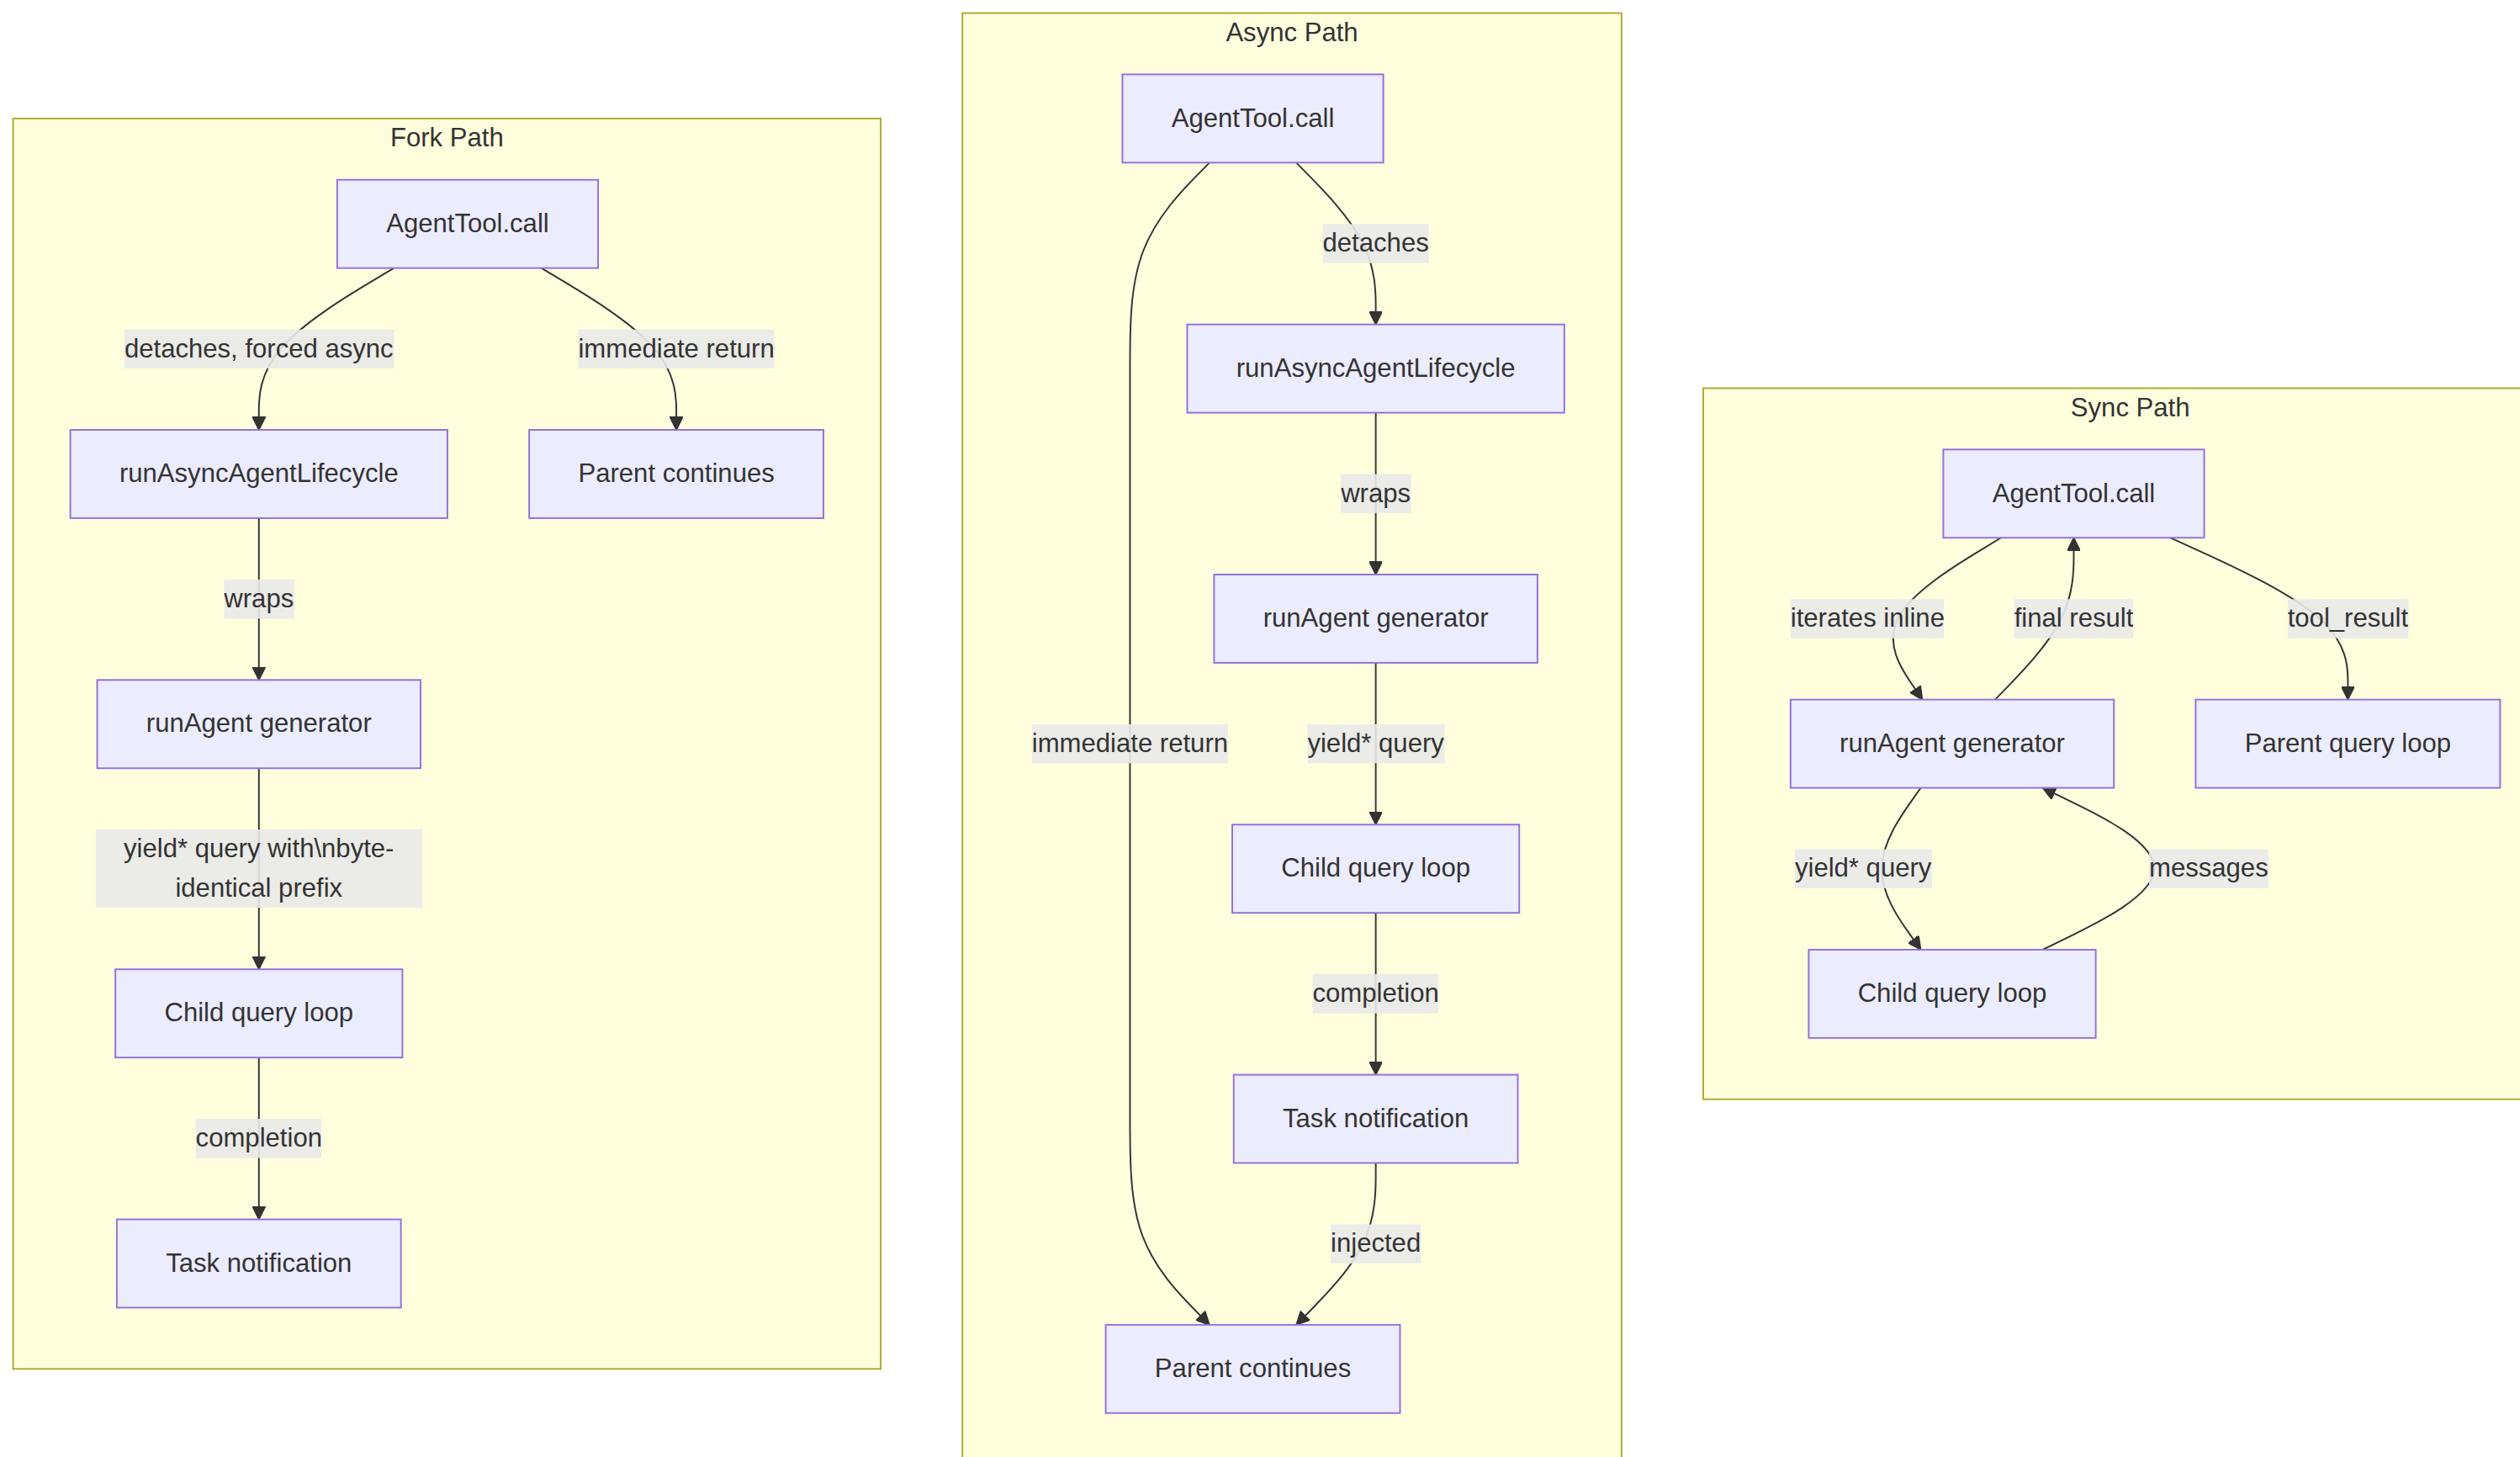
\includegraphics[width=16.38in,height=9.48in]{book/ch08-sub-agents_files/figure-latex/mermaid-figure-1.png}

This generator-based architecture enables four critical capabilities:

\textbf{Streaming.} Messages flow through the system incrementally. The
parent (or the async lifecycle wrapper) can observe each message as it
is produced -- updating progress indicators, forwarding metrics,
recording transcripts -- without buffering the entire conversation.

\textbf{Cancellation.} Returning the async iterator triggers the
\texttt{finally} block in \texttt{runAgent()}. The fifteen-step cleanup
runs regardless of whether the agent completed normally, was aborted by
the user, or threw an error. JavaScript's async generator protocol
guarantees this.

\textbf{Backgrounding.} A sync agent that is taking too long can be
backgrounded mid-execution. The iterator is handed off from the
foreground (where \texttt{AgentTool.call()} is iterating it) to an async
context (where \texttt{runAsyncAgentLifecycle()} takes over). The agent
does not restart -- it continues from where it was.

\textbf{Progress tracking.} Each yielded message is an observation
point. The async lifecycle wrapper uses these observation points to
update the task state machine, compute progress percentages, and
generate notifications when the agent completes.

\begin{center}\rule{0.5\linewidth}{0.5pt}\end{center}

\section{Built-In Agent Types}\label{built-in-agent-types}

Built-in agents are registered via \texttt{getBuiltInAgents()} in
\texttt{builtInAgents.ts}. The registry is dynamic -- which agents are
available depends on feature flags, GrowthBook experiments, and the
session's entrypoint type. Six built-in agents ship with the system,
each optimized for a specific class of work.

\subsection{General-Purpose}\label{general-purpose}

The default agent when \texttt{subagent\_type} is omitted and fork is
not active. Full tool access, no CLAUDE.md omission, model determined by
\texttt{getDefaultSubagentModel()}. Its system prompt positions it as a
completion-oriented worker: ``Complete the task fully -- don't
gold-plate, but don't leave it half-done.'' It includes guidelines for
search strategy (broad first, then narrow) and file creation discipline
(never create files unless the task requires it).

This is the workhorse. When the model does not know what kind of agent
it needs, it gets a general-purpose agent that can do everything the
parent can do, minus spawning its own sub-agents. The ``minus spawning''
restriction is important: without it, a general-purpose child could
spawn its own children, which could spawn theirs, creating an
exponential fan-out that burns through API budget in seconds. The
\texttt{Agent} tool is in the default disallowed list for good reason.

\subsection{Explore}\label{explore}

A read-only search specialist. Uses Haiku (the cheapest, fastest model).
Omits CLAUDE.md and git status. Has \texttt{FileEdit},
\texttt{FileWrite}, \texttt{NotebookEdit}, and \texttt{Agent} removed
from its tool pool, enforced at both the tooling level and via a
\texttt{===\ CRITICAL:\ READ-ONLY\ MODE\ ===} section in its system
prompt.

The Explore agent is the most aggressively optimized built-in because it
is the most frequently spawned -- 34 million times per week across the
fleet. It is marked as a one-shot agent
(\texttt{ONE\_SHOT\_BUILTIN\_AGENT\_TYPES}), which means the agentId,
SendMessage instructions, and usage trailer are skipped from its prompt,
saving approximately 135 characters per invocation. At 34 million
invocations, those 135 characters add up to roughly 4.6 billion
characters per week of saved prompt tokens.

Availability is gated by the \texttt{BUILTIN\_EXPLORE\_PLAN\_AGENTS}
feature flag AND the \texttt{tengu\_amber\_stoat} GrowthBook experiment,
which A/B tests the impact of removing these specialized agents.

\subsection{Plan}\label{plan}

A software architect agent. Same read-only tool set as Explore but uses
\texttt{\textquotesingle{}inherit\textquotesingle{}} for its model (same
capability as the parent). Its system prompt guides it through a
structured four-step process: Understand Requirements, Explore
Thoroughly, Design Solution, Detail the Plan. It must end with a
``Critical Files for Implementation'' list.

The Plan agent inherits the parent's model because architecture requires
the same reasoning capability as implementation. You do not want a
Haiku-class model making design decisions that an Opus-class model will
have to execute. The model mismatch would produce plans that the
executing agent cannot follow -- or worse, plans that sound plausible
but are subtly wrong in ways that only a more capable model would catch.

Same availability gate as Explore
(\texttt{BUILTIN\_EXPLORE\_PLAN\_AGENTS} +
\texttt{tengu\_amber\_stoat}).

\subsection{Verification}\label{verification}

The adversarial tester. Read-only tools,
\texttt{\textquotesingle{}inherit\textquotesingle{}} model, always runs
in background (\texttt{background:\ true}), displayed in red in the
terminal. Its system prompt is the most elaborate of any built-in agent
at approximately 130 lines.

What makes the Verification agent interesting is its anti-avoidance
programming. The prompt explicitly lists excuses the model might reach
for and instructs it to ``recognize them and do the opposite.'' Every
check must include a ``Command run'' block with actual terminal output
-- no hand-waving, no ``this should work.'' The agent must include at
least one adversarial probe (concurrency, boundary, idempotency, orphan
cleanup). And before reporting a failure, it must check whether the
behavior is intentional or handled elsewhere.

The \texttt{criticalSystemReminder\_EXPERIMENTAL} field injects a
reminder after every tool result, reinforcing that this is
verification-only. This is a guardrail against the model drifting from
``verify'' to ``fix'' -- a tendency that would undermine the entire
purpose of an independent verification pass. Language models have a
strong inclination to be helpful, and ``helpful'' in most contexts means
``fix the problem.'' The Verification agent's entire value proposition
depends on resisting that inclination.

The \texttt{background:\ true} flag means the Verification agent always
runs asynchronously. The parent does not wait for verification results
-- it continues working while the verifier probes in the background.
When the verifier finishes, a notification appears with the results.
This mirrors how human code review works: the developer does not stop
coding while the reviewer reads their PR.

Availability is gated by the \texttt{VERIFICATION\_AGENT} feature flag
AND the \texttt{tengu\_hive\_evidence} GrowthBook experiment.

\subsection{Claude Code Guide}\label{claude-code-guide}

A documentation-fetching agent for questions about Claude Code itself,
the Claude Agent SDK, and the Claude API. Uses Haiku, runs with
\texttt{dontAsk} permission mode (no user prompts needed -- it only
reads documentation), and has two hardcoded documentation URLs.

Its \texttt{getSystemPrompt()} is unique because it receives the
\texttt{toolUseContext} and dynamically includes context about the
project's custom skills, custom agents, configured MCP servers, plugin
commands, and user settings. This lets it answer ``how do I configure
X?'' by knowing what is already configured.

Excluded when the entrypoint is SDK (TypeScript, Python, or CLI), since
SDK users are not asking Claude Code how to use Claude Code. They are
building their own tools on top of it.

The Guide agent is an interesting case study in agent design because it
is the only built-in agent whose system prompt is dynamic in a way that
depends on the user's project. It needs to know what is configured to
answer ``how do I configure X?'' effectively. This makes its
\texttt{getSystemPrompt()} function more complex than the others, but
the trade-off is worth it -- a documentation agent that does not know
what the user has already set up gives worse answers than one that does.

\subsection{Statusline Setup}\label{statusline-setup}

A specialized agent for configuring the terminal status line. Uses
Sonnet, displayed in orange, limited to \texttt{Read} and \texttt{Edit}
tools only. Knows how to convert shell PS1 escape sequences to shell
commands, write to \texttt{\textasciitilde{}/.claude/settings.json}, and
handle the \texttt{statusLine} command's JSON input format.

This is the most narrowly-scoped built-in agent -- it exists because
status line configuration is a self-contained domain with specific
formatting rules that would clutter a general-purpose agent's context.
Always available, no feature gate.

The Statusline Setup agent illustrates an important principle:
\textbf{sometimes a specialized agent is better than a general-purpose
agent with more context.} A general-purpose agent given the status line
documentation as context would probably configure it correctly. But it
would also be more expensive (bigger model), slower (more context to
process), and more likely to get confused by the interaction between
status line syntax and the task at hand. A dedicated Sonnet agent with
Read and Edit tools and a focused system prompt does the job faster,
cheaper, and more reliably.

\subsection{The Worker Agent (Coordinator
Mode)}\label{the-worker-agent-coordinator-mode}

Not in the \texttt{built-in/} directory but loaded dynamically when
coordinator mode is active:

\begin{Shaded}
\begin{Highlighting}[]
\ControlFlowTok{if}\NormalTok{ (}\FunctionTok{isEnvTruthy}\NormalTok{(}\BuiltInTok{process}\OperatorTok{.}\AttributeTok{env}\OperatorTok{.}\AttributeTok{CLAUDE\_CODE\_COORDINATOR\_MODE}\NormalTok{)) \{}
  \KeywordTok{const}\NormalTok{ \{ getCoordinatorAgents \} }\OperatorTok{=} \PreprocessorTok{require}\NormalTok{(}\StringTok{\textquotesingle{}../../coordinator/workerAgent.js\textquotesingle{}}\NormalTok{)}
  \ControlFlowTok{return} \FunctionTok{getCoordinatorAgents}\NormalTok{()}
\NormalTok{\}}
\end{Highlighting}
\end{Shaded}

The worker agent replaces all standard built-in agents in coordinator
mode. It has a single type \texttt{"worker"} and full tool access. This
simplification is deliberate -- when a coordinator is orchestrating
workers, the coordinator decides what each worker does. The worker does
not need the specialization of Explore or Plan; it needs the flexibility
to do whatever the coordinator assigns.

\begin{center}\rule{0.5\linewidth}{0.5pt}\end{center}

\section{Fork Agents}\label{fork-agents}

Fork agents -- where the child inherits the parent's full conversation
history, system prompt, and tool array for prompt cache exploitation --
are the subject of Chapter 9. The fork path triggers when the model
omits \texttt{subagent\_type} from the Agent tool call and the fork
experiment is active. Every design decision in the fork system traces
back to a single goal: byte-identical API request prefixes across
parallel children, enabling 90\% cache discounts on shared context.

\begin{center}\rule{0.5\linewidth}{0.5pt}\end{center}

\section{Agent Definitions from
Frontmatter}\label{agent-definitions-from-frontmatter}

Users and plugins can define custom agents by placing markdown files in
\texttt{.claude/agents/}. The frontmatter schema supports the full range
of agent configuration:

\begin{Shaded}
\begin{Highlighting}[]
\PreprocessorTok{{-}{-}{-}}
\FunctionTok{description}\KeywordTok{:}\AttributeTok{ }\StringTok{"When to use this agent"}
\FunctionTok{tools}\KeywordTok{:}
\AttributeTok{  }\KeywordTok{{-}}\AttributeTok{ Read}
\AttributeTok{  }\KeywordTok{{-}}\AttributeTok{ Bash}
\AttributeTok{  }\KeywordTok{{-}}\AttributeTok{ Grep}
\FunctionTok{disallowedTools}\KeywordTok{:}
\AttributeTok{  }\KeywordTok{{-}}\AttributeTok{ FileWrite}
\FunctionTok{model}\KeywordTok{:}\AttributeTok{ haiku}
\FunctionTok{permissionMode}\KeywordTok{:}\AttributeTok{ dontAsk}
\FunctionTok{maxTurns}\KeywordTok{:}\AttributeTok{ }\DecValTok{50}
\FunctionTok{skills}\KeywordTok{:}
\AttributeTok{  }\KeywordTok{{-}}\AttributeTok{ my{-}custom{-}skill}
\FunctionTok{mcpServers}\KeywordTok{:}
\AttributeTok{  }\KeywordTok{{-}}\AttributeTok{ slack}
\AttributeTok{  }\KeywordTok{{-}}\AttributeTok{ }\FunctionTok{my{-}inline{-}server}\KeywordTok{:}
\AttributeTok{      }\FunctionTok{command}\KeywordTok{:}\AttributeTok{ node}
\AttributeTok{      }\FunctionTok{args}\KeywordTok{:}\AttributeTok{ }\KeywordTok{[}\StringTok{"./server.js"}\KeywordTok{]}
\FunctionTok{hooks}\KeywordTok{:}
\AttributeTok{  }\FunctionTok{PreToolUse}\KeywordTok{:}
\AttributeTok{    }\KeywordTok{{-}}\AttributeTok{ }\FunctionTok{command}\KeywordTok{:}\AttributeTok{ }\StringTok{"echo validating"}
\AttributeTok{      }\FunctionTok{event}\KeywordTok{:}\AttributeTok{ PreToolUse}
\FunctionTok{color}\KeywordTok{:}\AttributeTok{ blue}
\FunctionTok{background}\KeywordTok{:}\AttributeTok{ }\CharTok{false}
\FunctionTok{isolation}\KeywordTok{:}\AttributeTok{ worktree}
\FunctionTok{effort}\KeywordTok{:}\AttributeTok{ high}
\PreprocessorTok{{-}{-}{-}}

\CommentTok{\# My Custom Agent}

\AttributeTok{You are a specialized agent for...}
\end{Highlighting}
\end{Shaded}

The markdown body becomes the agent's system prompt. The frontmatter
fields map directly to the \texttt{AgentDefinition} interface that
\texttt{runAgent()} consumes. The loading pipeline in
\texttt{loadAgentsDir.ts} validates the frontmatter against
\texttt{AgentJsonSchema}, resolves the source (user, plugin, or policy),
and registers the agent in the available agents list.

Four sources of agent definitions exist, in priority order:

\begin{enumerate}
\def\labelenumi{\arabic{enumi}.}
\tightlist
\item
  \textbf{Built-in agents} -- hardcoded in TypeScript, always available
  (subject to feature gates)
\item
  \textbf{User agents} -- markdown files in \texttt{.claude/agents/}
\item
  \textbf{Plugin agents} -- loaded via \texttt{loadPluginAgents()}
\item
  \textbf{Policy agents} -- loaded via organizational policy settings
\end{enumerate}

When the model calls \texttt{Agent} with a \texttt{subagent\_type}, the
system resolves the name against this combined list, filtering by
permission rules (deny rules for \texttt{Agent(AgentName)}) and by
\texttt{allowedAgentTypes} from the tool spec. If the requested agent
type is not found or is denied, the tool call fails with an error.

This design means that organizations can ship custom agents via plugins
(a code review agent, a security audit agent, a deployment agent) and
have them appear seamlessly alongside the built-in agents. The model
sees them in the same list, with the same interface, and delegates to
them the same way.

The power of frontmatter-defined agents is that they require zero
TypeScript. A team lead who wants a ``PR review'' agent writes a
markdown file with the right frontmatter, drops it in
\texttt{.claude/agents/}, and it appears in every team member's agent
list on their next session. The system prompt is the markdown body. The
tool restrictions, model preference, and permission mode are declared in
YAML. The \texttt{runAgent()} lifecycle handles everything else -- the
same fifteen steps, the same cleanup, the same isolation guarantees.

This also means that agent definitions are version-controlled alongside
the codebase. A repository can ship agents tailored to its architecture,
conventions, and tooling. The agents evolve with the code. When the team
adopts a new testing framework, the verification agent's prompt is
updated in the same commit that adds the framework dependency.

There is one important security consideration: the trust boundary. User
agents (from \texttt{.claude/agents/}) are user-controlled -- their
hooks, MCP servers, and tool configurations are subject to
\texttt{strictPluginOnlyCustomization} restrictions when those policies
are active. Plugin agents and policy agents are admin-trusted and bypass
these restrictions. Built-in agents are part of the Claude Code binary
itself. The system tracks the \texttt{source} of each agent definition
precisely so that security policies can distinguish between ``the user
wrote this'' and ``the organization approved this.''

The \texttt{source} field is not just metadata -- it gates real
behavior. When a plugin-only policy is active for MCP, user agent
frontmatter that declares MCP servers is silently skipped (the MCP
connections are not established). When a plugin-only policy is active
for hooks, user agent frontmatter hooks are not registered. The agent
still runs -- it just runs without the untrusted extensions. This is a
principle of graceful degradation: the agent is useful even when its
full capabilities are restricted by policy.

\begin{center}\rule{0.5\linewidth}{0.5pt}\end{center}

\section{Apply This: Designing Agent
Types}\label{apply-this-designing-agent-types}

The built-in agents demonstrate a pattern language for agent design. If
you are building a system that spawns sub-agents -- whether using Claude
Code's AgentTool directly or designing your own multi-agent architecture
-- the design space breaks down into five dimensions.

\subsection{Dimension 1: What Can It
See?}\label{dimension-1-what-can-it-see}

The combination of \texttt{omitClaudeMd}, git status stripping, and
skill preloading controls the agent's awareness. Read-only agents see
less (they do not need project conventions). Specialized agents see more
(preloaded skills inject domain knowledge).

The key insight is that context is not free. Every token in the system
prompt, user context, or conversation history costs money and displaces
working memory. Claude Code strips CLAUDE.md from Explore agents not
because those instructions are harmful, but because they are irrelevant
-- and irrelevance at 34 million spawns per week becomes a line item on
the infrastructure bill. When designing your own agent types, ask:
``What does this agent need to know to do its job?'' and strip
everything else.

\subsection{Dimension 2: What Can It
Do?}\label{dimension-2-what-can-it-do}

The \texttt{tools} and \texttt{disallowedTools} fields set hard
boundaries. The Verification agent cannot edit files. The Explore agent
cannot write anything. The General-Purpose agent can do everything
except spawn sub-agents of its own.

Tool restrictions serve two purposes: \textbf{safety} (the Verification
agent cannot accidentally ``fix'' what it finds, preserving its
independence) and \textbf{focus} (an agent with fewer tools spends less
time deciding which tool to use). The pattern of combining tool-level
restrictions with system prompt guidance (Explore's
\texttt{===\ CRITICAL:\ READ-ONLY\ MODE\ ===}) is defense in depth --
the tools enforce the boundary mechanically, and the prompt explains
\emph{why} the boundary exists so the model does not waste turns trying
to work around it.

\subsection{Dimension 3: How Does It Interact with the
User?}\label{dimension-3-how-does-it-interact-with-the-user}

The \texttt{permissionMode} and \texttt{canShowPermissionPrompts}
settings determine whether the agent asks for permission, auto-denies,
or bubbles prompts to the parent's terminal. Background agents that
cannot interrupt the user must either work within pre-approved
boundaries or bubble.

The \texttt{awaitAutomatedChecksBeforeDialog} setting is a nuance worth
understanding. Background agents that \emph{can} show prompts (bubble
mode) wait for the classifier and permission hooks to run before
interrupting the user. This means the user is only interrupted for
genuinely ambiguous permissions -- not for things the automated system
could have resolved. In a multi-agent system where five background
agents are running simultaneously, this is the difference between a
usable interface and a permission-prompt barrage.

\subsection{Dimension 4: How Does It Relate to the
Parent?}\label{dimension-4-how-does-it-relate-to-the-parent}

Sync agents block the parent and share its state. Async agents run
independently with their own abort controller. Fork agents inherit the
full conversation context. The choice shapes both the user experience
(does the parent wait?) and the system behavior (does Escape kill the
child?).

The abort controller decision in Step 8 crystallizes this: sync agents
share the parent's controller (Escape kills both), async agents get
their own (Escape leaves them running). Fork agents go further -- they
inherit the parent's system prompt, tool array, and message history to
maximize prompt cache sharing. Each relationship type has a clear use
case: sync for sequential delegation (``do this then I'll continue''),
async for parallel work (``do this while I do something else''), and
fork for context-heavy delegation (``you know everything I know, now go
handle this part'').

\subsection{Dimension 5: How Expensive Is
It?}\label{dimension-5-how-expensive-is-it}

The model choice, thinking config, and context size all contribute to
cost. Haiku for cheap read-only work. Sonnet for moderate tasks.
Inherit-from-parent for tasks requiring the parent's reasoning
capability. Thinking is disabled for non-fork agents to control output
token costs -- the parent pays for reasoning; the children execute.

The economic dimension is often an afterthought in multi-agent system
design, but it is central to Claude Code's architecture. An Explore
agent that used Opus instead of Haiku would work fine for any individual
invocation. But at 34 million invocations per week, the model choice is
a multiplicative cost factor. The one-shot optimization that saves 135
characters per Explore invocation translates to 4.6 billion characters
per week of saved prompt tokens. These are not micro-optimizations --
they are the difference between a viable product and an unaffordable
one.

\subsection{The Unified Lifecycle}\label{the-unified-lifecycle}

The \texttt{runAgent()} lifecycle implements all five dimensions through
its fifteen steps, assembling a unique execution environment for each
agent type from the same set of building blocks. The result is a system
where spawning a sub-agent is not ``run another copy of the parent.'' It
is the creation of a precisely-scoped, resource-controlled, isolated
execution context -- tailored to the work at hand, and cleaned up
completely when the work is done.

The architectural elegance is in the uniformity. Whether the agent is a
Haiku-powered read-only searcher or an Opus-powered fork child with full
tool access and bubble permissions, it flows through the same fifteen
steps. The steps do not branch based on agent type -- they parameterize.
Model resolution picks the right model. Context preparation picks the
right file state. Permission isolation picks the right mode. The agent
type is not encoded in control flow; it is encoded in configuration. And
that is what makes the system extensible: adding a new agent type means
writing a definition, not modifying the lifecycle.

\subsection{The Design Space
Summarized}\label{the-design-space-summarized}

The six built-in agents cover a spectrum:

\begin{longtable}[]{@{}
  >{\raggedright\arraybackslash}p{(\linewidth - 10\tabcolsep) * \real{0.1373}}
  >{\raggedright\arraybackslash}p{(\linewidth - 10\tabcolsep) * \real{0.1373}}
  >{\raggedright\arraybackslash}p{(\linewidth - 10\tabcolsep) * \real{0.1373}}
  >{\raggedright\arraybackslash}p{(\linewidth - 10\tabcolsep) * \real{0.1765}}
  >{\raggedright\arraybackslash}p{(\linewidth - 10\tabcolsep) * \real{0.2353}}
  >{\raggedright\arraybackslash}p{(\linewidth - 10\tabcolsep) * \real{0.1765}}@{}}
\toprule\noalign{}
\begin{minipage}[b]{\linewidth}\raggedright
Agent
\end{minipage} & \begin{minipage}[b]{\linewidth}\raggedright
Model
\end{minipage} & \begin{minipage}[b]{\linewidth}\raggedright
Tools
\end{minipage} & \begin{minipage}[b]{\linewidth}\raggedright
Context
\end{minipage} & \begin{minipage}[b]{\linewidth}\raggedright
Sync/Async
\end{minipage} & \begin{minipage}[b]{\linewidth}\raggedright
Purpose
\end{minipage} \\
\midrule\noalign{}
\endhead
\bottomrule\noalign{}
\endlastfoot
General-Purpose & Default & All & Full & Either & Workhorse
delegation \\
Explore & Haiku & Read-only & Stripped & Sync & Fast, cheap search \\
Plan & Inherit & Read-only & Stripped & Sync & Architecture design \\
Verification & Inherit & Read-only & Full & Always async & Adversarial
testing \\
Guide & Haiku & Read + Web & Dynamic & Sync & Documentation lookup \\
Statusline & Sonnet & Read + Edit & Minimal & Sync & Config task \\
\end{longtable}

No two agents make the same choices across all five dimensions. Each is
optimized for its specific use case. And the \texttt{runAgent()}
lifecycle handles all of them through the same fifteen steps,
parameterized by the agent definition. This is the power of the
architecture: the lifecycle is a universal machine, and the agent
definitions are the programs that run on it.

The next chapter examines fork agents in depth -- the prompt cache
exploitation mechanism that makes parallel delegation economically
viable. Chapter 10 then follows with the orchestration layer: how async
agents report progress through the task state machine, how the parent
retrieves results, and how the coordinator pattern orchestrates dozens
of agents working toward a single goal. If this chapter was about
\emph{creating} agents, Chapter 9 is about making them cheap, and
Chapter 10 is about \emph{managing} them.

\chapter{Chapter 9: Fork Agents and the Prompt
Cache}\label{chapter-9-fork-agents-and-the-prompt-cache}

\section{The Ninety-Five Percent
Insight}\label{the-ninety-five-percent-insight}

When a parent agent spawns five child agents in parallel, the
overwhelming majority of each child's API request is identical. The
system prompt is the same. The tool definitions are the same. The
conversation history is the same. The assistant message that triggered
the spawns is the same. The only thing that differs is the final
directive: ``you handle the database migration,'' ``you write the
tests,'' ``you update the docs.''

On a typical fork with a warm conversation, the shared prefix might be
80,000 tokens. The per-child directive might be 200 tokens. That is
99.75\% overlap. Anthropic's prompt cache gives a 90\% discount on
cached input tokens. If you can make those 80,000 tokens hit the cache
for children 2 through 5, you just cut the input cost of those four
requests by 90\%. For the parent, this is the difference between
spending \$4 and spending \$0.50 on the same parallel dispatch.

The catch is that prompt caching is byte-exact. Not ``similar enough.''
Not ``semantically equivalent.'' The bytes must match, character for
character, from the first byte of the system prompt through to the last
byte before the per-child content diverges. One extra space, one
reordered tool definition, one stale feature flag changing a system
prompt fragment -- and the cache misses. The entire prefix is
reprocessed at full price.

Fork agents are Claude Code's answer to this constraint. They are not
just a convenience for ``spawn a child with context'' -- they are a
prompt cache exploitation mechanism disguised as an orchestration
feature. Every design decision in the fork system traces back to one
question: how do we guarantee byte-identical prefixes across parallel
children?

\begin{center}\rule{0.5\linewidth}{0.5pt}\end{center}

\section{What a Fork Child Inherits}\label{what-a-fork-child-inherits}

A fork agent inherits four things from its parent, and it inherits them
by reference or byte-exact copy, not by recomputation.

\textbf{1. The system prompt.} Not regenerated -- threaded. The parent's
already-rendered system prompt bytes are passed via
\texttt{override.systemPrompt}, pulled from
\texttt{toolUseContext.renderedSystemPrompt}. This is the exact string
that was sent in the parent's most recent API call.

\textbf{2. The tool definitions.} The fork agent definition declares
\texttt{tools:\ {[}\textquotesingle{}*\textquotesingle{}{]}}, but with
the \texttt{useExactTools} flag set to true, the child receives the
parent's assembled tool array directly. No filtering, no reordering, no
re-serialization.

\textbf{3. The conversation history.} Every message the parent has
exchanged with the API -- user turns, assistant turns, tool calls, tool
results -- is cloned into the child's context via
\texttt{forkContextMessages}.

\textbf{4. The thinking configuration and model.} The fork definition
specifies \texttt{model:\ \textquotesingle{}inherit\textquotesingle{}},
which resolves to the parent's exact model. Same model means same
tokenizer, same context window, same cache namespace.

The fork agent definition itself is minimal -- almost a no-op:

The fork agent definition is deliberately minimal -- it inherits
everything from the parent. It specifies all tools
(\texttt{\textquotesingle{}*\textquotesingle{}}), inherits the parent's
model, uses bubble mode for permissions (so prompts surface in the
parent's terminal), and provides a no-op system prompt function that is
never actually called -- the real prompt arrives via the override
channel, already rendered and byte-stable.

\begin{center}\rule{0.5\linewidth}{0.5pt}\end{center}

\section{The Byte-Identical Prefix
Trick}\label{the-byte-identical-prefix-trick}

The API request to Claude has a specific structure: system prompt, then
tools, then messages. For the prompt cache to hit, every byte from the
start of the request through to some prefix boundary must be identical
across requests.

Fork agents achieve this by ensuring three layers are frozen:

\textbf{Layer 1: System prompt via threading, not recomputation.}

When the parent agent's system prompt was rendered for its last API
call, the result was captured in
\texttt{toolUseContext.renderedSystemPrompt}. This is the string after
all dynamic interpolation -- GrowthBook feature flags, environment
details, MCP server descriptions, skill content, CLAUDE.md files. The
fork child receives this exact string.

Why not just call \texttt{getSystemPrompt()} again? Because system
prompt generation is not pure. GrowthBook flags transition from cold to
warm state as the SDK fetches remote config. A flag that returned
\texttt{false} during the parent's first turn might return \texttt{true}
by the time the fork child spins up. If the system prompt includes a
conditional block gated by that flag, the re-rendered prompt diverges by
even a single character. Cache busted. Full-price reprocessing of 80,000
tokens, times five children.

Threading the rendered bytes eliminates this entire class of divergence.

\textbf{Layer 2: Tool definitions via exact passthrough.}

Normal sub-agents go through \texttt{resolveAgentTools()}, which filters
the tool pool based on the agent definition's \texttt{tools} and
\texttt{disallowedTools} arrays, applies permission mode differences,
and potentially reorders tools. The resulting serialized tool array
would differ from the parent's -- different subset, different order,
different permission annotations.

Fork agents skip this entirely:

\begin{Shaded}
\begin{Highlighting}[]
\KeywordTok{const}\NormalTok{ resolvedTools }\OperatorTok{=}\NormalTok{ useExactTools}
  \OperatorTok{?}\NormalTok{ availableTools  }\CommentTok{// parent\textquotesingle{}s exact array}
  \OperatorTok{:} \FunctionTok{resolveAgentTools}\NormalTok{(agentDefinition}\OperatorTok{,}\NormalTok{ availableTools}\OperatorTok{,}\NormalTok{ isAsync)}\OperatorTok{.}\AttributeTok{resolvedTools}
\end{Highlighting}
\end{Shaded}

The \texttt{useExactTools} flag is set to true only on the fork path.
The child gets the parent's tool pool as-is. Same tools, same order,
same serialization. This includes keeping the Agent tool itself in the
child's pool, even though the child is forbidden from using it --
removing it would change the tool array and bust the cache.

\textbf{Layer 3: Message array construction.}

This is where \texttt{buildForkedMessages()} does its careful work. The
function constructs the final two messages that sit between the shared
history and the per-child directive:

The \texttt{buildForkedMessages()} function constructs the final two
messages that sit between the shared history and the per-child
directive. The algorithm:

\begin{enumerate}
\def\labelenumi{\arabic{enumi}.}
\tightlist
\item
  Clone the parent's assistant message (preserving all
  \texttt{tool\_use} blocks with their original IDs).
\item
  For each \texttt{tool\_use} block, create a \texttt{tool\_result} with
  a constant placeholder string (identical across all children).
\item
  Build a single user message containing all the placeholder results
  followed by the per-child directive wrapped in the boilerplate tag.
\item
  Return
  \texttt{{[}clonedAssistantMessage,\ userMessageWithPlaceholdersAndDirective{]}}.
\end{enumerate}

\begin{Shaded}
\begin{Highlighting}[]
\CommentTok{// Pseudocode — illustrates the message construction}
\KeywordTok{function} \FunctionTok{buildChildMessages}\NormalTok{(directive}\OperatorTok{,}\NormalTok{ parentAssistant) \{}
  \KeywordTok{const}\NormalTok{ cloned }\OperatorTok{=} \FunctionTok{cloneMessage}\NormalTok{(parentAssistant)}
  \KeywordTok{const}\NormalTok{ placeholders }\OperatorTok{=}\NormalTok{ parentAssistant}\OperatorTok{.}\AttributeTok{toolUseBlocks}\OperatorTok{.}\FunctionTok{map}\NormalTok{(b }\KeywordTok{=\textgreater{}}
    \FunctionTok{toolResult}\NormalTok{(b}\OperatorTok{.}\AttributeTok{id}\OperatorTok{,}\NormalTok{ CONSTANT\_PLACEHOLDER)  }\CommentTok{// Byte{-}identical across children}
\NormalTok{  )}
  \KeywordTok{const}\NormalTok{ userMsg }\OperatorTok{=} \FunctionTok{createUserMessage}\NormalTok{([}\OperatorTok{...}\NormalTok{placeholders}\OperatorTok{,} \FunctionTok{wrapDirective}\NormalTok{(directive)])}
  \ControlFlowTok{return}\NormalTok{ [cloned}\OperatorTok{,}\NormalTok{ userMsg]}
\NormalTok{\}}
\end{Highlighting}
\end{Shaded}

The resulting message array for each child looks like:

\begin{verbatim}
[...shared_history, assistant(all_tool_uses), user(placeholder_results..., directive)]
\end{verbatim}

Every element before the directive is identical across children. The
\texttt{FORK\_PLACEHOLDER\_RESULT} -- a constant string
\texttt{\textquotesingle{}Fork\ started\ -\/-\ processing\ in\ background\textquotesingle{}}
-- ensures even the tool result blocks are byte-identical. The
\texttt{tool\_use\_id} values are identical because they reference the
same assistant message. Only the final text block, containing the
per-child directive, varies.

The cache boundary falls right before that final text block. Everything
above it -- potentially tens of thousands of tokens of system prompt,
tool definitions, conversation history, and placeholder results -- hits
the cache at a 90\% discount for every child after the first.

\begin{center}\rule{0.5\linewidth}{0.5pt}\end{center}

\section{The Fork Boilerplate Tag}\label{the-fork-boilerplate-tag}

Each child's directive is wrapped in a boilerplate XML tag that serves
two purposes: it instructs the child on how to behave, and it acts as a
marker for recursive fork detection.

The boilerplate contains approximately 10 rules. The key ones:

\begin{itemize}
\tightlist
\item
  \textbf{Override the parent's forking instruction.} The parent's
  system prompt says ``default to forking'' -- the boilerplate
  explicitly tells the child: ``that instruction is for the parent. You
  ARE the fork. Do NOT spawn sub-agents.''
\item
  \textbf{Execute silently, report once.} No conversational text between
  tool calls. Use tools directly, then produce a structured summary.
\item
  \textbf{Stay within scope.} The child must not expand beyond its
  directive.
\item
  \textbf{Structured output format.} The response must follow a
  Scope/Result/Key files/Files changed/Issues template that makes
  results easy for the parent to parse when multiple children report
  back simultaneously.
\end{itemize}

Rule 1 is particularly interesting. The parent's system prompt -- which
the fork child inherits verbatim for cache reasons -- contains
instructions like ``default to forking when you have parallel work.'' If
the child followed that instruction, it would try to fork its own
children, creating an infinite recursion of agents. The boilerplate
explicitly overrides: ``that instruction is for the parent. You ARE the
fork.''

The structured output format (Scope/Result/Key files/Files
changed/Issues) is not decorative. It constrains the child's output to
factual reporting, which makes the results easier for the parent to
parse and aggregate when five children report back simultaneously.

\begin{center}\rule{0.5\linewidth}{0.5pt}\end{center}

\section{Recursive Fork Prevention}\label{recursive-fork-prevention}

The fork child keeps the Agent tool in its tool pool. It has to --
removing it would change the serialized tool array and bust the prompt
cache. But if the child actually invokes the Agent tool without
\texttt{subagent\_type}, the fork path would trigger again, creating a
grandchild fork. This grandchild would inherit an even larger context
(parent + child conversation), spawn its own forks, and so on.

Two guards prevent this:

\textbf{Primary guard: querySource check.} When a fork child is spawned,
its \texttt{context.options.querySource} is set to
\texttt{\textquotesingle{}agent:builtin:fork\textquotesingle{}}. The
\texttt{call()} method checks this before allowing the fork path:

\begin{Shaded}
\begin{Highlighting}[]
\CommentTok{// In AgentTool.call():}
\ControlFlowTok{if}\NormalTok{ (effectiveType }\OperatorTok{===} \KeywordTok{undefined}\NormalTok{) \{}
  \CommentTok{// Fork path {-}{-} but are we already in a fork?}
  \ControlFlowTok{if}\NormalTok{ (querySource }\OperatorTok{===} \StringTok{\textquotesingle{}agent:builtin:fork\textquotesingle{}}\NormalTok{) \{}
    \CommentTok{// Reject: already a fork child}
\NormalTok{  \}}
\NormalTok{\}}
\end{Highlighting}
\end{Shaded}

This is the fast path. It checks a single string in the options object.

\textbf{Fallback guard: message scanning.} Fork prevention uses two
guards: the \texttt{querySource} tag set at spawn time (the fast path --
a single string comparison), and a fallback that scans message history
for the boilerplate XML tag. The fallback exists because the
\texttt{querySource} survives autocompact, but in edge cases where it
was not properly threaded, the message-scanning fallback catches the
recursion. It is a belt-and-suspenders approach where the cost of the
check (scanning messages) is trivial compared to the cost of accidental
recursive forking (runaway API spend).

Why the fallback? Because Claude Code has an autocompact feature that
rewrites the message array when context gets too long. Autocompact can
rewrite message content but preserves the \texttt{querySource} in
options. In theory, \texttt{querySource} alone is sufficient. In
practice, the message-scanning fallback catches edge cases where
\texttt{querySource} was not properly threaded -- a belt-and-suspenders
approach where the cost of the check (scanning messages) is trivial
compared to the cost of accidental recursive forking (runaway API
spend).

\begin{center}\rule{0.5\linewidth}{0.5pt}\end{center}

\section{The Sync-to-Async
Transition}\label{the-sync-to-async-transition}

A fork child starts running in the foreground: its messages stream to
the parent's terminal, and the parent blocks waiting for completion. But
what if the child is taking too long? Claude Code allows mid-execution
backgrounding -- the user (or an auto-timeout) can push a running
foreground agent into the background without losing any work.

The mechanism is surprisingly clean:

\begin{enumerate}
\def\labelenumi{\arabic{enumi}.}
\item
  When a foreground agent is registered via
  \texttt{registerAgentForeground()}, a background signal promise is
  created.
\item
  The parent's sync loop races between the agent's message stream and
  the background signal:
\end{enumerate}

\begin{verbatim}
while (true) {
  const result = await Promise.race([
    iterator.next(),         // next message from agent
    backgroundSignal,        // "move to background" trigger
  ])
  if (result === BACKGROUND_SIGNAL) break
  // ... process message
}
\end{verbatim}

\begin{enumerate}
\def\labelenumi{\arabic{enumi}.}
\setcounter{enumi}{2}
\item
  When the background signal fires, the foreground iterator is
  gracefully terminated via \texttt{iterator.return()}. This triggers
  the generator's \texttt{finally} block, which handles cleanup.
\item
  A new \texttt{runAgent()} instance is spawned with
  \texttt{isAsync:\ true}, using the same agent ID and the message
  history accumulated so far. The agent continues from where it left
  off, now running in the background.
\item
  The original synchronous \texttt{call()} returns
  \texttt{\{\ status:\ \textquotesingle{}async\_launched\textquotesingle{}\ \}},
  and the parent continues its conversation.
\end{enumerate}

No work is lost because the message history is the agent's state. The
sidechain transcript on disk has every message the agent has produced.
The new async instance replays from this transcript and picks up where
the sync instance stopped.

\begin{center}\rule{0.5\linewidth}{0.5pt}\end{center}

\section{Auto-Backgrounding}\label{auto-backgrounding}

When the \texttt{CLAUDE\_AUTO\_BACKGROUND\_TASKS} environment variable
or the \texttt{tengu\_auto\_background\_agents} GrowthBook flag is
enabled, foreground agents are automatically backgrounded after 120
seconds:

When enabled via environment variable or feature flag, foreground agents
are automatically backgrounded after 120 seconds. When disabled, the
function returns 0 (no auto-backgrounding).

This is a UX decision with cost implications. A foreground agent blocks
the parent terminal -- the user cannot type, cannot issue new
instructions, cannot spawn other agents. Two minutes is long enough for
the agent to complete most quick tasks synchronously (where the
streaming output is useful feedback), but short enough that long-running
tasks do not hold the terminal hostage.

Under the fork experiment, the auto-backgrounding question is moot: all
fork spawns are forced async from the start. The
\texttt{run\_in\_background} parameter is hidden from the schema
entirely. Every fork child runs in the background, reports back via a
\texttt{\textless{}task-notification\textgreater{}} when done, and the
parent never blocks.

\begin{center}\rule{0.5\linewidth}{0.5pt}\end{center}

\section{When Fork Is NOT Used}\label{when-fork-is-not-used}

Fork is one of several orchestration modes, and it is deliberately
excluded in three cases:

\textbf{Coordinator mode.} Coordinator mode and fork mode are mutually
exclusive. A coordinator has a structured delegation model: it maintains
a plan, assigns tasks to workers with explicit prompts, and tracks
progress. Fork's ``inherit everything'' approach would undermine this. A
forked coordinator would inherit the parent coordinator's system prompt
(which says ``you are the coordinator, delegate work''), and the child
would try to orchestrate instead of execute. The
\texttt{isForkSubagentEnabled()} function checks
\texttt{isCoordinatorMode()} first and returns false if active.

\textbf{Non-interactive sessions.} SDK and API consumers
(\texttt{-\/-print} mode, Claude Agent SDK) operate without a terminal.
Fork's
\texttt{permissionMode:\ \textquotesingle{}bubble\textquotesingle{}}
surfaces permission prompts to the parent terminal -- which does not
exist in non-interactive mode. Rather than building a separate
permission flow, the fork path is simply disabled. SDK consumers use
explicit \texttt{subagent\_type} selection instead.

\textbf{Explicit subagent\_type.} When the model specifies a
\texttt{subagent\_type} (e.g., \texttt{"Explore"}, \texttt{"Plan"},
\texttt{"general-purpose"}), the fork path is not triggered. Fork only
fires when \texttt{subagent\_type} is omitted. This lets the model
choose between ``I want a specialized agent with its own system prompt
and tool set'' (explicit type) and ``I want a context-inheriting clone
of myself to handle this in parallel'' (omitted type).

\begin{center}\rule{0.5\linewidth}{0.5pt}\end{center}

\section{The Economics}\label{the-economics}

Consider a concrete scenario. A developer asks Claude Code to refactor a
module. The parent agent analyzes the codebase, forms a plan, and
dispatches five fork children in parallel: one to update the database
schema, one to rewrite the service layer, one to update the router, one
to fix the tests, and one to update the types.

At this point in the conversation, the shared context is substantial: -
System prompt: \textasciitilde4,000 tokens - Tool definitions (40+
tools): \textasciitilde12,000 tokens - Conversation history (analysis +
planning): \textasciitilde30,000 tokens - Assistant message with five
tool\_use blocks: \textasciitilde2,000 tokens - Placeholder tool
results: \textasciitilde500 tokens

Total shared prefix: \textasciitilde48,500 tokens. Per-child directive:
\textasciitilde200 tokens.

Without fork (five independent agents, each with fresh context and their
own system prompt): - Each child processes its own system prompt + tools
+ task prompt - No cache sharing (different system prompts, different
tool sets) - Cost: 5 x full input processing

With fork (byte-identical prefixes): - Child 1: 48,700 tokens at full
price (cache miss on first request) - Children 2-5: 48,500 tokens at
10\% price (cache hit) + 200 tokens at full price each - Effective cost
for children 2-5: \textasciitilde4,850 + 200 = \textasciitilde5,050
tokens equivalent each

The savings scale with context size and child count. For a warm session
with 100K tokens of history spawning 8 parallel forks, the cache savings
can exceed 90\% of what the input tokens would have cost without
sharing.

This is why every design decision in the fork system -- the threading
instead of recomputation, the exact tool passthrough, the placeholder
results, even keeping the Agent tool in the child's pool despite it
being forbidden -- optimizes for one thing: byte-identical prefixes.
Each decision trades a small amount of elegance or safety for a
measurable reduction in API cost.

\begin{center}\rule{0.5\linewidth}{0.5pt}\end{center}

\section{Design Tensions}\label{design-tensions}

The fork system makes explicit trade-offs that are worth understanding:

\textbf{Isolation vs.~cache efficiency.} Fork children inherit
everything, including conversation history that may be irrelevant to
their task. A child rewriting tests does not need the 15 messages where
the parent discussed database schema design. But including those
messages is what makes the prefix identical. Stripping irrelevant
history would save context window space at the cost of busting the
cache. The design bet is that cache savings outweigh the context
overhead.

\textbf{Safety vs.~cache efficiency.} The Agent tool stays in the fork
child's tool pool even though the child must not use it. Removing it
would be safer (the child cannot even attempt to fork), but would change
the tool array serialization. The boilerplate tag and recursive fork
guards are the compensating controls -- runtime prevention instead of
static removal.

\textbf{Simplicity vs.~cache efficiency.} The placeholder tool results
are a lie. The child sees
\texttt{\textquotesingle{}Fork\ started\ -\/-\ processing\ in\ background\textquotesingle{}}
for every tool\_use block in the parent's assistant message, regardless
of what those tool calls actually did. This is fine because the child's
directive tells it what to do -- it does not need accurate tool results
from the parent's dispatching turn. But it means the child's
conversation history is technically incoherent. The placeholder is
chosen for brevity and uniformity, not accuracy.

Each of these trade-offs reflects the same priority: when you are paying
per-token for API calls at scale, byte-identical prefixes are worth
contorting the architecture around.

\begin{center}\rule{0.5\linewidth}{0.5pt}\end{center}

\section{Apply This: Designing for Prompt Cache
Efficiency}\label{apply-this-designing-for-prompt-cache-efficiency}

The fork agent pattern generalizes beyond Claude Code. Any system that
dispatches multiple parallel LLM calls from the same context can benefit
from cache-aware request construction. The principles:

\textbf{1. Thread rendered prompts, do not recompute.} If your system
prompt includes any dynamic content -- feature flags, timestamps, user
preferences, A/B test variants -- capture the rendered result and pass
it to children by value. Recomputing risks divergence.

\textbf{2. Freeze the tool array.} If your children need different tool
sets, you are giving up cache sharing on the tools block. Consider
keeping the full tool set and using runtime guards (like the fork
boilerplate's ``do not use Agent'') instead of compile-time removal.

\textbf{3. Maximize the shared prefix, minimize the per-child suffix.}
Structure your message array so that everything shared comes first and
per-child content is appended at the end. Interleaving shared and
per-child content fragments the cache boundary.

\textbf{4. Use constant placeholders for variable content.} When the
message structure requires responses to previous tool calls, use
identical placeholder strings across all children rather than actual
(divergent) results.

\textbf{5. Measure the break-even.} Cache sharing has overhead: larger
context windows per child (they carry irrelevant history), runtime
guards instead of static safety, architectural complexity. Calculate
whether your parallelism pattern (how many children, how large the
shared prefix) actually saves money after accounting for the extra
context tokens.

The fork agent system is, at its core, a prompt cache exploitation
engine. It answers a question that every multi-agent system builder
eventually faces: when the cache gives you a 90\% discount on repeated
prefixes, how far will you restructure your architecture to claim that
discount? Claude Code's answer is: very far.

\chapter{Chapter 10: Tasks, Coordination, and
Swarms}\label{chapter-10-tasks-coordination-and-swarms}

\section{The Limits of a Single
Thread}\label{the-limits-of-a-single-thread}

Chapter 8 showed how to create a sub-agent -- the fifteen-step lifecycle
that builds an isolated execution context from an agent definition.
Chapter 9 showed how to make parallel spawns economical through prompt
cache exploitation. But creating agents and managing agents are
different problems. This chapter addresses the second.

A single agent loop -- one model, one conversation, one tool at a time
-- can accomplish a remarkable amount of work. It can read files, edit
code, run tests, search the web, and reason about complex problems. But
it hits a ceiling.

The ceiling is not intelligence. It is parallelism and scope. A
developer working on a large refactoring needs to update 40 files, run
tests after each batch, and verify nothing broke. A codebase migration
touches frontend, backend, and database layers simultaneously. A
thorough code review reads dozens of files while running the test suite
in the background. These are not harder problems -- they are wider ones.
They require the ability to do multiple things at once, to delegate work
to specialists, and to coordinate the results.

Claude Code's answer to this problem is not one mechanism but a layered
stack of orchestration patterns, each suited to a different shape of
work. Background tasks for fire-and-forget commands. Coordinator mode
for manager-worker hierarchies. Swarm teams for peer-to-peer
collaboration. And a unified communication protocol that ties them all
together.

The orchestration layer spans approximately 40 files across
\texttt{tools/AgentTool/}, \texttt{tasks/}, \texttt{coordinator/},
\texttt{tools/SendMessageTool/}, and \texttt{utils/swarm/}. Despite this
breadth, the design is anchored by a single state machine that all
patterns share. Understanding that state machine -- the \texttt{Task}
abstraction in \texttt{Task.ts} -- is the prerequisite for understanding
everything else.

This chapter traces the full stack, from the foundational task state
machine up through the most sophisticated multi-agent topologies.

\begin{center}\rule{0.5\linewidth}{0.5pt}\end{center}

\section{The Task State Machine}\label{the-task-state-machine}

Every background operation in Claude Code -- a shell command, a
sub-agent, a remote session, a workflow script -- is tracked as a
\emph{task}. The task abstraction lives in \texttt{Task.ts} and provides
the unified state model that the rest of the orchestration layer builds
on.

\subsection{Seven Types}\label{seven-types}

The system defines seven task types, each representing a different
execution model:

The seven task types are: \texttt{local\_bash} (background shell
commands), \texttt{local\_agent} (background sub-agents),
\texttt{remote\_agent} (remote sessions), \texttt{in\_process\_teammate}
(swarm teammates), \texttt{local\_workflow} (workflow script
executions), \texttt{monitor\_mcp} (MCP server monitors), and
\texttt{dream} (speculative background thinking).

\texttt{local\_bash} and \texttt{local\_agent} are the workhorses --
background shell commands and background sub-agents, respectively.
\texttt{in\_process\_teammate} is the swarm primitive.
\texttt{remote\_agent} bridges to remote Claude Code Runtime
environments. \texttt{local\_workflow} runs multi-step scripts.
\texttt{monitor\_mcp} watches MCP server health. \texttt{dream} is the
most unusual -- a background task that lets the agent think
speculatively while waiting for user input.

Each type gets a single-character ID prefix for instant visual
identification:

\begin{longtable}[]{@{}lll@{}}
\toprule\noalign{}
Type & Prefix & Example ID \\
\midrule\noalign{}
\endhead
\bottomrule\noalign{}
\endlastfoot
\texttt{local\_bash} & \texttt{b} & \texttt{b4k2m8x1} \\
\texttt{local\_agent} & \texttt{a} & \texttt{a7j3n9p2} \\
\texttt{remote\_agent} & \texttt{r} & \texttt{r1h5q6w4} \\
\texttt{in\_process\_teammate} & \texttt{t} & \texttt{t3f8s2v5} \\
\texttt{local\_workflow} & \texttt{w} & \texttt{w6c9d4y7} \\
\texttt{monitor\_mcp} & \texttt{m} & \texttt{m2g7k1z8} \\
\texttt{dream} & \texttt{d} & \texttt{d5b4n3r6} \\
\end{longtable}

Task IDs use a single-character prefix (a for agents, b for bash, t for
teammates, etc.) followed by 8 random alphanumeric characters drawn from
a case-insensitive-safe alphabet (digits plus lowercase letters). This
yields approximately 2.8 trillion combinations -- enough to resist
brute-force symlink attacks against the task output files on disk.

When you see \texttt{a7j3n9p2} in a log line, you know immediately it is
a background agent. When you see \texttt{b4k2m8x1}, a shell command. The
prefix is a micro-optimization for human readers, but in a system that
can have dozens of concurrent tasks, it matters.

\subsection{Five Statuses}\label{five-statuses}

The lifecycle is a simple directed graph with no cycles:

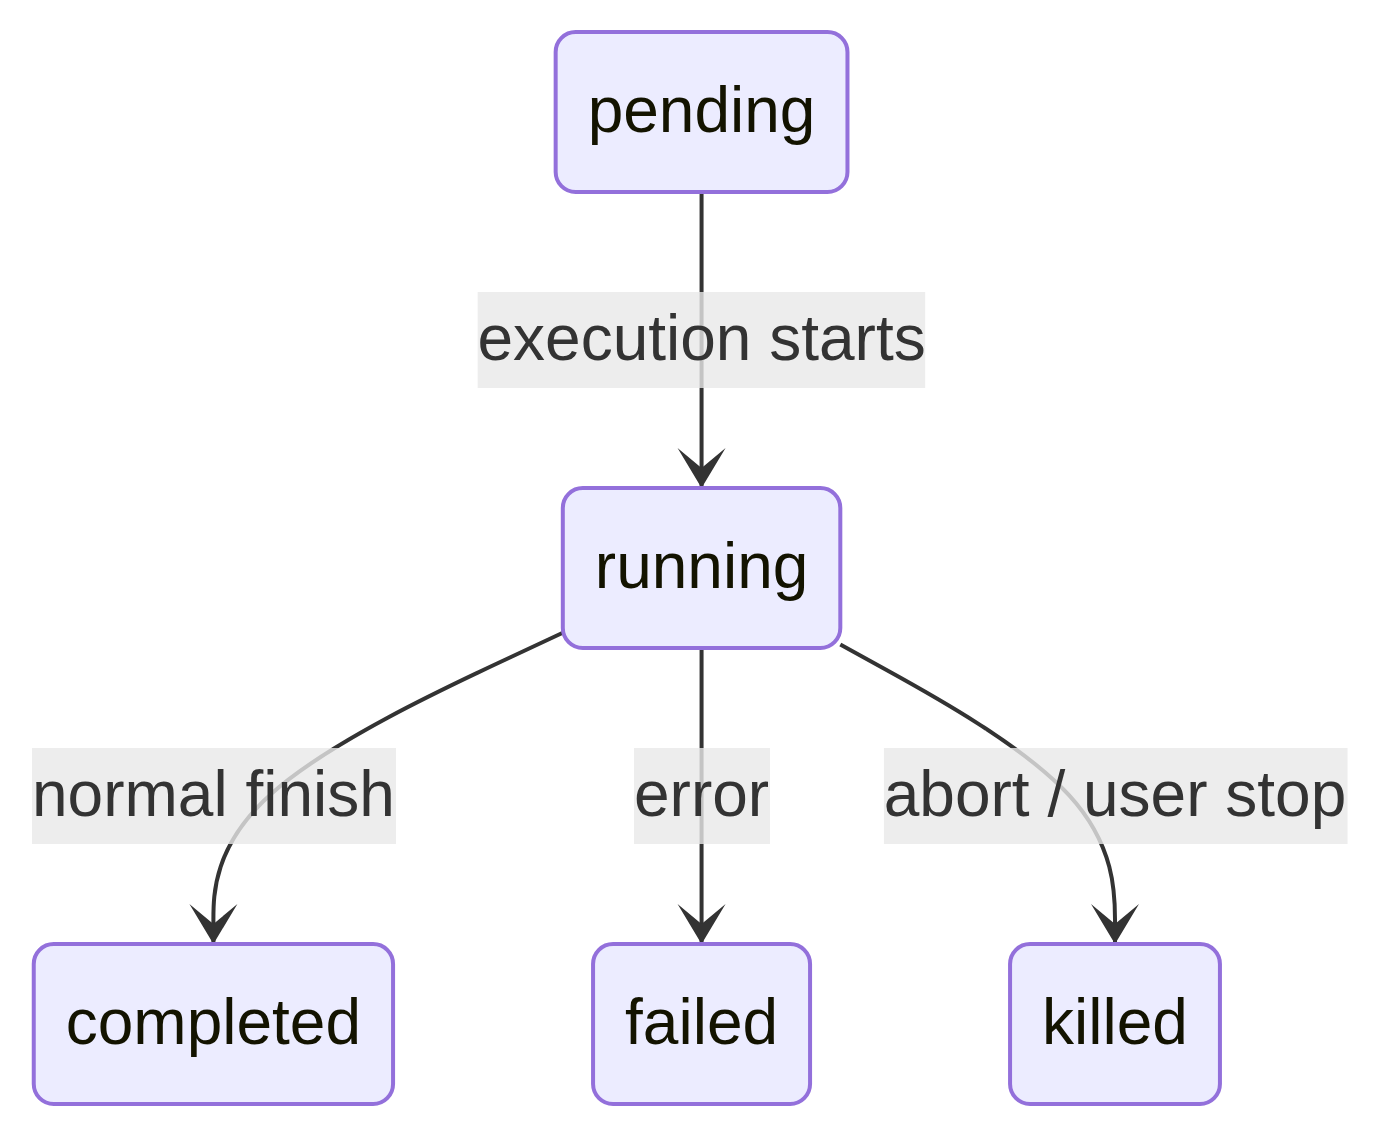
\includegraphics[width=3.59in,height=2.96in]{book/ch10-coordination_files/figure-latex/mermaid-figure-1.png}

\texttt{pending} is the brief state between registration and first
execution. \texttt{running} means the task is actively doing work. The
three terminal states are \texttt{completed} (success), \texttt{failed}
(error), and \texttt{killed} (explicitly stopped by the user, the
coordinator, or an abort signal). A helper function guards against
interacting with dead tasks:

\begin{Shaded}
\begin{Highlighting}[]
\ImportTok{export} \KeywordTok{function} \FunctionTok{isTerminalTaskStatus}\NormalTok{(status}\OperatorTok{:}\NormalTok{ TaskStatus)}\OperatorTok{:} \DataTypeTok{boolean}\NormalTok{ \{}
  \ControlFlowTok{return}\NormalTok{ status }\OperatorTok{===} \StringTok{\textquotesingle{}completed\textquotesingle{}} \OperatorTok{||}\NormalTok{ status }\OperatorTok{===} \StringTok{\textquotesingle{}failed\textquotesingle{}} \OperatorTok{||}\NormalTok{ status }\OperatorTok{===} \StringTok{\textquotesingle{}killed\textquotesingle{}}
\NormalTok{\}}
\end{Highlighting}
\end{Shaded}

This function appears everywhere -- in message injection guards,
eviction logic, orphan cleanup, and the SendMessage routing that decides
whether to queue a message or resume a dead agent.

\subsection{The Base State}\label{the-base-state}

Every task state extends \texttt{TaskStateBase}, which carries the
fields that all seven types share:

\begin{Shaded}
\begin{Highlighting}[]
\ImportTok{export type}\NormalTok{ TaskStateBase }\OperatorTok{=}\NormalTok{ \{}
\NormalTok{  id}\OperatorTok{:} \DataTypeTok{string}              \CommentTok{// Prefixed random ID}
\NormalTok{  type}\OperatorTok{:}\NormalTok{ TaskType          }\CommentTok{// Discriminator}
\NormalTok{  status}\OperatorTok{:}\NormalTok{ TaskStatus      }\CommentTok{// Current lifecycle position}
\NormalTok{  description}\OperatorTok{:} \DataTypeTok{string}     \CommentTok{// Human{-}readable summary}
\NormalTok{  toolUseId}\OperatorTok{?:} \DataTypeTok{string}      \CommentTok{// The tool\_use block that spawned this task}
\NormalTok{  startTime}\OperatorTok{:} \DataTypeTok{number}       \CommentTok{// Creation timestamp}
\NormalTok{  endTime}\OperatorTok{?:} \DataTypeTok{number}        \CommentTok{// Terminal{-}state timestamp}
\NormalTok{  totalPausedMs}\OperatorTok{?:} \DataTypeTok{number}  \CommentTok{// Accumulated pause time}
\NormalTok{  outputFile}\OperatorTok{:} \DataTypeTok{string}      \CommentTok{// Disk path for streaming output}
\NormalTok{  outputOffset}\OperatorTok{:} \DataTypeTok{number}    \CommentTok{// Read cursor for incremental output}
\NormalTok{  notified}\OperatorTok{:} \DataTypeTok{boolean}       \CommentTok{// Whether completion was reported to parent}
\NormalTok{\}}
\end{Highlighting}
\end{Shaded}

Two fields deserve attention. \texttt{outputFile} is the bridge between
async execution and the parent's conversation -- every task writes its
output to a file on disk, and the parent can read it incrementally via
\texttt{outputOffset}. \texttt{notified} prevents duplicate completion
messages; once the parent has been told a task finished, the flag flips
to \texttt{true} and the notification is never sent again. Without this
guard, a task that completes between two consecutive polls of the
notification queue would generate duplicate notifications, confusing the
model into thinking two tasks finished when only one did.

\subsection{The Agent Task State}\label{the-agent-task-state}

\texttt{LocalAgentTaskState} is the most complex variant, carrying
everything needed to manage a background sub-agent's full lifecycle:

\begin{Shaded}
\begin{Highlighting}[]
\ImportTok{export type}\NormalTok{ LocalAgentTaskState }\OperatorTok{=}\NormalTok{ TaskStateBase }\OperatorTok{\&}\NormalTok{ \{}
\NormalTok{  type}\OperatorTok{:} \StringTok{\textquotesingle{}local\_agent\textquotesingle{}}
\NormalTok{  agentId}\OperatorTok{:} \DataTypeTok{string}
\NormalTok{  prompt}\OperatorTok{:} \DataTypeTok{string}
\NormalTok{  selectedAgent}\OperatorTok{?:}\NormalTok{ AgentDefinition}
\NormalTok{  agentType}\OperatorTok{:} \DataTypeTok{string}
\NormalTok{  model}\OperatorTok{?:} \DataTypeTok{string}
\NormalTok{  abortController}\OperatorTok{?:}\NormalTok{ AbortController}
\NormalTok{  pendingMessages}\OperatorTok{:} \DataTypeTok{string}\NormalTok{[]       }\CommentTok{// Queued via SendMessage}
\NormalTok{  isBackgrounded}\OperatorTok{:} \DataTypeTok{boolean}         \CommentTok{// Was this originally a foreground agent?}
\NormalTok{  retain}\OperatorTok{:} \DataTypeTok{boolean}                 \CommentTok{// UI is holding this task}
\NormalTok{  diskLoaded}\OperatorTok{:} \DataTypeTok{boolean}             \CommentTok{// Sidechain transcript loaded}
\NormalTok{  evictAfter}\OperatorTok{?:} \DataTypeTok{number}             \CommentTok{// GC deadline}
\NormalTok{  progress}\OperatorTok{?:}\NormalTok{ AgentProgress}
\NormalTok{  lastReportedToolCount}\OperatorTok{:} \DataTypeTok{number}
\NormalTok{  lastReportedTokenCount}\OperatorTok{:} \DataTypeTok{number}
  \CommentTok{// ... additional lifecycle fields}
\NormalTok{\}}
\end{Highlighting}
\end{Shaded}

Three fields reveal important design decisions. \texttt{pendingMessages}
is the inbox -- when \texttt{SendMessage} targets a running agent, the
message is queued here rather than injected immediately. Messages are
drained at tool-round boundaries, which preserves the agent's turn
structure. \texttt{isBackgrounded} distinguishes agents that were born
async from those that started as foreground sync agents and were later
backgrounded by the user pressing a key. \texttt{evictAfter} is a
garbage collection mechanism: non-retained completed tasks get a grace
period before their state is purged from memory.

All task states are stored in \texttt{AppState.tasks} as a
\texttt{Record\textless{}string,\ TaskState\textgreater{}}, keyed by the
prefixed ID. This is a flat map, not a tree -- the system does not model
parent-child relationships in the state store. The parent-child
relationship is implicit in the conversation flow: the parent holds the
\texttt{toolUseId} that spawned the child.

\subsection{The Task Registry}\label{the-task-registry}

Each task type is backed by a \texttt{Task} object with a minimal
interface:

\begin{Shaded}
\begin{Highlighting}[]
\ImportTok{export type}\NormalTok{ Task }\OperatorTok{=}\NormalTok{ \{}
\NormalTok{  name}\OperatorTok{:} \DataTypeTok{string}
\NormalTok{  type}\OperatorTok{:}\NormalTok{ TaskType}
  \FunctionTok{kill}\NormalTok{(taskId}\OperatorTok{:} \DataTypeTok{string}\OperatorTok{,}\NormalTok{ setAppState}\OperatorTok{:}\NormalTok{ SetAppState)}\OperatorTok{:} \BuiltInTok{Promise}\OperatorTok{\textless{}}\DataTypeTok{void}\OperatorTok{\textgreater{}}
\NormalTok{\}}
\end{Highlighting}
\end{Shaded}

The registry collects all task implementations:

\begin{Shaded}
\begin{Highlighting}[]
\ImportTok{export} \KeywordTok{function} \FunctionTok{getAllTasks}\NormalTok{()}\OperatorTok{:}\NormalTok{ Task[] \{}
  \ControlFlowTok{return}\NormalTok{ [}
\NormalTok{    LocalShellTask}\OperatorTok{,}
\NormalTok{    LocalAgentTask}\OperatorTok{,}
\NormalTok{    RemoteAgentTask}\OperatorTok{,}
\NormalTok{    DreamTask}\OperatorTok{,}
    \OperatorTok{...}\NormalTok{(LocalWorkflowTask }\OperatorTok{?}\NormalTok{ [LocalWorkflowTask] }\OperatorTok{:}\NormalTok{ [])}\OperatorTok{,}
    \OperatorTok{...}\NormalTok{(MonitorMcpTask }\OperatorTok{?}\NormalTok{ [MonitorMcpTask] }\OperatorTok{:}\NormalTok{ [])}\OperatorTok{,}
\NormalTok{  ]}
\NormalTok{\}}
\end{Highlighting}
\end{Shaded}

Notice the conditional inclusion -- \texttt{LocalWorkflowTask} and
\texttt{MonitorMcpTask} are feature-gated and may not exist at runtime.
The \texttt{Task} interface is deliberately minimal. Earlier iterations
included \texttt{spawn()} and \texttt{render()} methods, but these were
removed when it became clear that spawning and rendering were never
called polymorphically. Each task type has its own spawn logic, its own
state management, and its own rendering. The only operation that
genuinely needs to dispatch by type is \texttt{kill()}, and so that is
all the interface requires.

This is an example of interface evolution through subtraction. The
initial design imagined that all task types would share a common
lifecycle interface. In practice, the types diverged enough that the
shared interface became a fiction -- \texttt{spawn()} for a shell
command and \texttt{spawn()} for an in-process teammate have almost
nothing in common. Rather than maintain a leaky abstraction, the team
removed everything except the one method that actually benefits from
polymorphism.

\begin{center}\rule{0.5\linewidth}{0.5pt}\end{center}

\section{Communication Patterns}\label{communication-patterns}

A task that runs in the background is only useful if the parent can
observe its progress and receive its results. Claude Code supports three
communication channels, each optimized for a different access pattern.

\subsection{Foreground: The Generator
Chain}\label{foreground-the-generator-chain}

When an agent runs synchronously, the parent iterates its
\texttt{runAgent()} async generator directly, yielding each message back
up the call stack. The interesting mechanism here is the background
escape hatch -- the sync loop races between ``next message from agent''
and ``background signal'':

\begin{Shaded}
\begin{Highlighting}[]
\KeywordTok{const}\NormalTok{ agentIterator }\OperatorTok{=} \FunctionTok{runAgent}\NormalTok{(\{ }\OperatorTok{...}\NormalTok{params \})[}\BuiltInTok{Symbol}\OperatorTok{.}\AttributeTok{asyncIterator}\NormalTok{]()}

\ControlFlowTok{while}\NormalTok{ (}\KeywordTok{true}\NormalTok{) \{}
  \KeywordTok{const}\NormalTok{ nextMessagePromise }\OperatorTok{=}\NormalTok{ agentIterator}\OperatorTok{.}\FunctionTok{next}\NormalTok{()}
  \KeywordTok{const}\NormalTok{ raceResult }\OperatorTok{=}\NormalTok{ backgroundPromise}
    \OperatorTok{?} \ControlFlowTok{await} \BuiltInTok{Promise}\OperatorTok{.}\FunctionTok{race}\NormalTok{([nextMessagePromise}\OperatorTok{.}\FunctionTok{then}\NormalTok{(}\OperatorTok{...}\NormalTok{)}\OperatorTok{,}\NormalTok{ backgroundPromise])}
    \OperatorTok{:}\NormalTok{ \{ type}\OperatorTok{:} \StringTok{\textquotesingle{}message\textquotesingle{}}\OperatorTok{,}\NormalTok{ result}\OperatorTok{:} \ControlFlowTok{await}\NormalTok{ nextMessagePromise \}}

  \ControlFlowTok{if}\NormalTok{ (raceResult}\OperatorTok{.}\AttributeTok{type} \OperatorTok{===} \StringTok{\textquotesingle{}background\textquotesingle{}}\NormalTok{) \{}
    \CommentTok{// User triggered backgrounding {-}{-} transition to async}
    \ControlFlowTok{await}\NormalTok{ agentIterator}\OperatorTok{.}\FunctionTok{return}\NormalTok{(}\KeywordTok{undefined}\NormalTok{)}
    \KeywordTok{void} \FunctionTok{runAgent}\NormalTok{(\{ }\OperatorTok{...}\NormalTok{params}\OperatorTok{,}\NormalTok{ isAsync}\OperatorTok{:} \KeywordTok{true}\NormalTok{ \})}
    \ControlFlowTok{return}\NormalTok{ \{ data}\OperatorTok{:}\NormalTok{ \{ status}\OperatorTok{:} \StringTok{\textquotesingle{}async\_launched\textquotesingle{}}\NormalTok{ \} \}}
\NormalTok{  \}}

\NormalTok{  agentMessages}\OperatorTok{.}\FunctionTok{push}\NormalTok{(message)}
\NormalTok{\}}
\end{Highlighting}
\end{Shaded}

If the user decides mid-execution that a sync agent should become a
background task, the foreground iterator is cleanly returned (triggering
its \texttt{finally} block for resource cleanup), and the agent is
re-spawned as an async task with the same ID. The transition is seamless
-- no work is lost, and the agent continues from where it left off with
an async abort controller that is unlinked from the parent's ESC key.

This is a genuinely difficult state transition to get right. The
foreground agent shares the parent's abort controller (ESC kills both).
The background agent needs its own controller (ESC should not kill it).
The agent's messages need to transfer from the foreground generator
stream to the background notification system. The task state needs to
flip \texttt{isBackgrounded} so the UI knows to show it in the
background panel. And all of this must happen atomically -- no messages
lost in the transition, no zombie iterators left running. The
\texttt{Promise.race} between the next message and the background signal
is the mechanism that makes this possible.

\subsection{Background: Three Channels}\label{background-three-channels}

Background agents communicate through disk, notifications, and queued
messages.

\textbf{Disk output files.} Every task writes to an \texttt{outputFile}
path -- a symlink to the agent's transcript in JSONL format. The parent
(or any observer) can read this file incrementally using
\texttt{outputOffset}, which tracks how far into the file has been
consumed. The \texttt{TaskOutputTool} exposes this to the model:

\begin{Shaded}
\begin{Highlighting}[]
\NormalTok{inputSchema }\OperatorTok{=}\NormalTok{ z}\OperatorTok{.}\FunctionTok{strictObject}\NormalTok{(\{}
\NormalTok{  task\_id}\OperatorTok{:}\NormalTok{ z}\OperatorTok{.}\FunctionTok{string}\NormalTok{()}\OperatorTok{,}
\NormalTok{  block}\OperatorTok{:}\NormalTok{ z}\OperatorTok{.}\FunctionTok{boolean}\NormalTok{()}\OperatorTok{.}\FunctionTok{default}\NormalTok{(}\KeywordTok{true}\NormalTok{)}\OperatorTok{,}
\NormalTok{  timeout}\OperatorTok{:}\NormalTok{ z}\OperatorTok{.}\FunctionTok{number}\NormalTok{()}\OperatorTok{.}\FunctionTok{default}\NormalTok{(}\DecValTok{30000}\NormalTok{)}\OperatorTok{,}
\NormalTok{\})}
\end{Highlighting}
\end{Shaded}

When \texttt{block:\ true}, the tool polls until the task reaches a
terminal state or the timeout expires. This is the primary mechanism for
a coordinator that spawns a worker and waits for its result.

\textbf{Task notifications.} When a background agent completes, the
system generates an XML notification and enqueues it for delivery into
the parent's conversation:

\begin{Shaded}
\begin{Highlighting}[]
\NormalTok{\textless{}}\KeywordTok{task{-}notification}\NormalTok{\textgreater{}}
\NormalTok{  \textless{}}\KeywordTok{task{-}id}\NormalTok{\textgreater{}a7j3n9p2\textless{}/}\KeywordTok{task{-}id}\NormalTok{\textgreater{}}
\NormalTok{  \textless{}}\KeywordTok{tool{-}use{-}id}\NormalTok{\textgreater{}toolu\_abc123\textless{}/}\KeywordTok{tool{-}use{-}id}\NormalTok{\textgreater{}}
\NormalTok{  \textless{}}\KeywordTok{output{-}file}\NormalTok{\textgreater{}/path/to/output\textless{}/}\KeywordTok{output{-}file}\NormalTok{\textgreater{}}
\NormalTok{  \textless{}}\KeywordTok{status}\NormalTok{\textgreater{}completed\textless{}/}\KeywordTok{status}\NormalTok{\textgreater{}}
\NormalTok{  \textless{}}\KeywordTok{summary}\NormalTok{\textgreater{}Agent "Investigate auth bug" completed\textless{}/}\KeywordTok{summary}\NormalTok{\textgreater{}}
\NormalTok{  \textless{}}\KeywordTok{result}\NormalTok{\textgreater{}Found null pointer in src/auth/validate.ts:42...\textless{}/}\KeywordTok{result}\NormalTok{\textgreater{}}
\NormalTok{  \textless{}}\KeywordTok{usage}\NormalTok{\textgreater{}}
\NormalTok{    \textless{}}\KeywordTok{total\_tokens}\NormalTok{\textgreater{}15000\textless{}/}\KeywordTok{total\_tokens}\NormalTok{\textgreater{}}
\NormalTok{    \textless{}}\KeywordTok{tool\_uses}\NormalTok{\textgreater{}8\textless{}/}\KeywordTok{tool\_uses}\NormalTok{\textgreater{}}
\NormalTok{    \textless{}}\KeywordTok{duration\_ms}\NormalTok{\textgreater{}12000\textless{}/}\KeywordTok{duration\_ms}\NormalTok{\textgreater{}}
\NormalTok{  \textless{}/}\KeywordTok{usage}\NormalTok{\textgreater{}}
\NormalTok{\textless{}/}\KeywordTok{task{-}notification}\NormalTok{\textgreater{}}
\end{Highlighting}
\end{Shaded}

The notification is injected as a user-role message in the parent's
conversation, which means the model sees it in its normal message flow.
It does not need a special tool to check for completions -- they arrive
as context. The \texttt{notified} flag on the task state prevents
duplicate delivery.

\textbf{Command queue.} The \texttt{pendingMessages} array on
\texttt{LocalAgentTaskState} is the third channel. When
\texttt{SendMessage} targets a running agent, the message is queued:

\begin{Shaded}
\begin{Highlighting}[]
\ControlFlowTok{if}\NormalTok{ (}\FunctionTok{isLocalAgentTask}\NormalTok{(task) }\OperatorTok{\&\&}\NormalTok{ task}\OperatorTok{.}\AttributeTok{status} \OperatorTok{===} \StringTok{\textquotesingle{}running\textquotesingle{}}\NormalTok{) \{}
  \FunctionTok{queuePendingMessage}\NormalTok{(agentId}\OperatorTok{,}\NormalTok{ input}\OperatorTok{.}\AttributeTok{message}\OperatorTok{,}\NormalTok{ setAppState)}
  \ControlFlowTok{return}\NormalTok{ \{ data}\OperatorTok{:}\NormalTok{ \{ success}\OperatorTok{:} \KeywordTok{true}\OperatorTok{,}\NormalTok{ message}\OperatorTok{:} \StringTok{\textquotesingle{}Message queued...\textquotesingle{}}\NormalTok{ \} \}}
\NormalTok{\}}
\end{Highlighting}
\end{Shaded}

These messages are drained at tool-round boundaries by
\texttt{drainPendingMessages()} and injected as user messages into the
agent's conversation. This is a crucial design choice -- messages arrive
between tool rounds, not mid-execution. The agent finishes its current
thought, then receives the new information. No race conditions, no
corrupted state.

\subsection{Progress Tracking}\label{progress-tracking}

The \texttt{ProgressTracker} provides real-time visibility into agent
activity:

\begin{Shaded}
\begin{Highlighting}[]
\ImportTok{export type}\NormalTok{ ProgressTracker }\OperatorTok{=}\NormalTok{ \{}
\NormalTok{  toolUseCount}\OperatorTok{:} \DataTypeTok{number}
\NormalTok{  latestInputTokens}\OperatorTok{:} \DataTypeTok{number}        \CommentTok{// Cumulative (latest value, not sum)}
\NormalTok{  cumulativeOutputTokens}\OperatorTok{:} \DataTypeTok{number}   \CommentTok{// Summed across turns}
\NormalTok{  recentActivities}\OperatorTok{:}\NormalTok{ ToolActivity[] }\CommentTok{// Last 5 tool uses}
\NormalTok{\}}
\end{Highlighting}
\end{Shaded}

The distinction between input and output token tracking is deliberate
and reflects a subtlety of the API's billing model. Input tokens are
cumulative per API call because the full conversation is re-sent each
time -- the 15th turn includes all 14 previous turns, so the input token
count reported by the API already reflects the total. Keeping the latest
value is the correct aggregation. Output tokens are per-turn -- the
model generates new tokens each time -- so summing is the correct
aggregation. Getting this wrong would either dramatically overcount
(summing cumulative input tokens) or dramatically undercount (keeping
only the latest output tokens).

The \texttt{recentActivities} array (capped at 5 entries) provides a
human-readable stream of what the agent is doing: ``Read
src/auth/validate.ts'', ``Bash: npm test'', ``Edit
src/auth/validate.ts''. This appears in the VS Code subagent panel and
the terminal's background task indicator, giving users visibility into
agent work without requiring them to read full transcripts.

For background agents, progress is written to \texttt{AppState} via
\texttt{updateAsyncAgentProgress()} and emitted as SDK events via
\texttt{emitTaskProgress()}. The VS Code subagent panel consumes these
events to render live progress bars, tool counts, and activity streams.
The progress tracking is not just cosmetic -- it is the primary feedback
mechanism that tells users whether a background agent is making progress
or stuck in a loop.

\begin{center}\rule{0.5\linewidth}{0.5pt}\end{center}

\section{Coordinator Mode}\label{coordinator-mode}

Coordinator mode transforms Claude Code from a single agent with
background helpers into a true manager-worker architecture. It is the
most opinionated orchestration pattern in the system, and its design
reveals deep thinking about how LLMs should and should not delegate
work.

\subsection{The Problem Coordinator Mode
Solves}\label{the-problem-coordinator-mode-solves}

The standard agent loop has a single conversation and a single context
window. When it spawns a background agent, the background agent runs
independently and reports results via task notifications. This works
well for simple delegation -- ``run the tests while I keep editing'' --
but breaks down for complex multi-step workflows.

Consider a codebase migration. The agent needs to: (1) understand the
current patterns across 200 files, (2) design the migration strategy,
(3) apply changes to each file, and (4) verify nothing broke. Steps 1
and 3 benefit from parallelism. Step 2 requires synthesizing the results
of step 1. Step 4 depends on step 3. A single agent doing this
sequentially would spend most of its token budget re-reading files.
Multiple background agents doing this without coordination would produce
inconsistent changes.

Coordinator mode solves this by splitting the ``thinking'' agent from
the ``doing'' agents. The coordinator handles steps 1 and 2 (dispatching
research workers, then synthesizing). Workers handle steps 3 and 4
(applying changes, running tests). The coordinator sees the full
picture; workers see their specific task.

\subsection{Activation}\label{activation}

A single environment variable flips the switch:

\begin{Shaded}
\begin{Highlighting}[]
\ImportTok{export} \KeywordTok{function} \FunctionTok{isCoordinatorMode}\NormalTok{()}\OperatorTok{:} \DataTypeTok{boolean}\NormalTok{ \{}
  \ControlFlowTok{if}\NormalTok{ (}\FunctionTok{feature}\NormalTok{(}\StringTok{\textquotesingle{}COORDINATOR\_MODE\textquotesingle{}}\NormalTok{)) \{}
    \ControlFlowTok{return} \FunctionTok{isEnvTruthy}\NormalTok{(}\BuiltInTok{process}\OperatorTok{.}\AttributeTok{env}\OperatorTok{.}\AttributeTok{CLAUDE\_CODE\_COORDINATOR\_MODE}\NormalTok{)}
\NormalTok{  \}}
  \ControlFlowTok{return} \KeywordTok{false}
\NormalTok{\}}
\end{Highlighting}
\end{Shaded}

On session resume, \texttt{matchSessionMode()} checks whether the
resumed session's stored mode matches the current environment. If they
diverge, the environment variable is flipped to match. This prevents the
confusing scenario where a coordinator session resumes as a regular
agent (losing awareness of its workers) or a regular session resumes as
a coordinator (losing access to its tools). The session's mode is the
source of truth; the environment variable is the runtime signal.

\subsection{Tool Restrictions}\label{tool-restrictions}

The coordinator's power comes not from having more tools, but from
having fewer. In coordinator mode, the coordinator agent gets exactly
three tools:

\begin{itemize}
\tightlist
\item
  \textbf{Agent} -- spawn workers
\item
  \textbf{SendMessage} -- communicate with existing workers
\item
  \textbf{TaskStop} -- terminate running workers
\end{itemize}

That is it. No file reading. No code editing. No shell commands. The
coordinator cannot directly touch the codebase. This restriction is not
a limitation -- it is the core design principle. The coordinator's job
is to think, plan, decompose, and synthesize. Workers do the work.

Workers, conversely, get the full tool set minus internal coordination
tools:

\begin{Shaded}
\begin{Highlighting}[]
\KeywordTok{const}\NormalTok{ INTERNAL\_WORKER\_TOOLS }\OperatorTok{=} \KeywordTok{new} \BuiltInTok{Set}\NormalTok{([}
\NormalTok{  TEAM\_CREATE\_TOOL\_NAME}\OperatorTok{,}
\NormalTok{  TEAM\_DELETE\_TOOL\_NAME}\OperatorTok{,}
\NormalTok{  SEND\_MESSAGE\_TOOL\_NAME}\OperatorTok{,}
\NormalTok{  SYNTHETIC\_OUTPUT\_TOOL\_NAME}\OperatorTok{,}
\NormalTok{])}
\end{Highlighting}
\end{Shaded}

Workers cannot spawn their own sub-teams or send messages to peers. They
report results through the normal task completion mechanism, and the
coordinator synthesizes across them.

\subsection{The 370-Line System
Prompt}\label{the-370-line-system-prompt}

The coordinator system prompt is, line for line, the most instructive
document in the codebase about how to use LLMs for orchestration. It
runs approximately 370 lines and encodes hard-won lessons about
delegation patterns. The key teachings:

\textbf{``Never delegate understanding.''} This is the central thesis.
The coordinator must synthesize research findings into specific prompts
with file paths, line numbers, and exact changes. The prompt explicitly
calls out anti-patterns like ``based on your findings, fix the bug'' --
a prompt that delegates \emph{comprehension} to the worker, forcing it
to re-derive context the coordinator already has. The correct pattern
is: ``In \texttt{src/auth/validate.ts} at line 42, the \texttt{userId}
parameter can be null when called from the OAuth flow. Add a null check
that returns a 401 response.''

\textbf{``Parallelism is your superpower.''} The prompt establishes a
clear concurrency model. Read-only tasks run freely in parallel --
research, exploration, file reading. Write-heavy tasks serialize per
file set. The coordinator is expected to reason about which tasks can
overlap and which must sequence. A good coordinator spawns five research
workers simultaneously, waits for all of them, synthesizes, then spawns
three implementation workers that touch disjoint file sets. A bad
coordinator spawns one worker, waits, spawns the next, waits again --
serializing work that could have been parallel.

\textbf{Task workflow phases.} The prompt defines four phases:

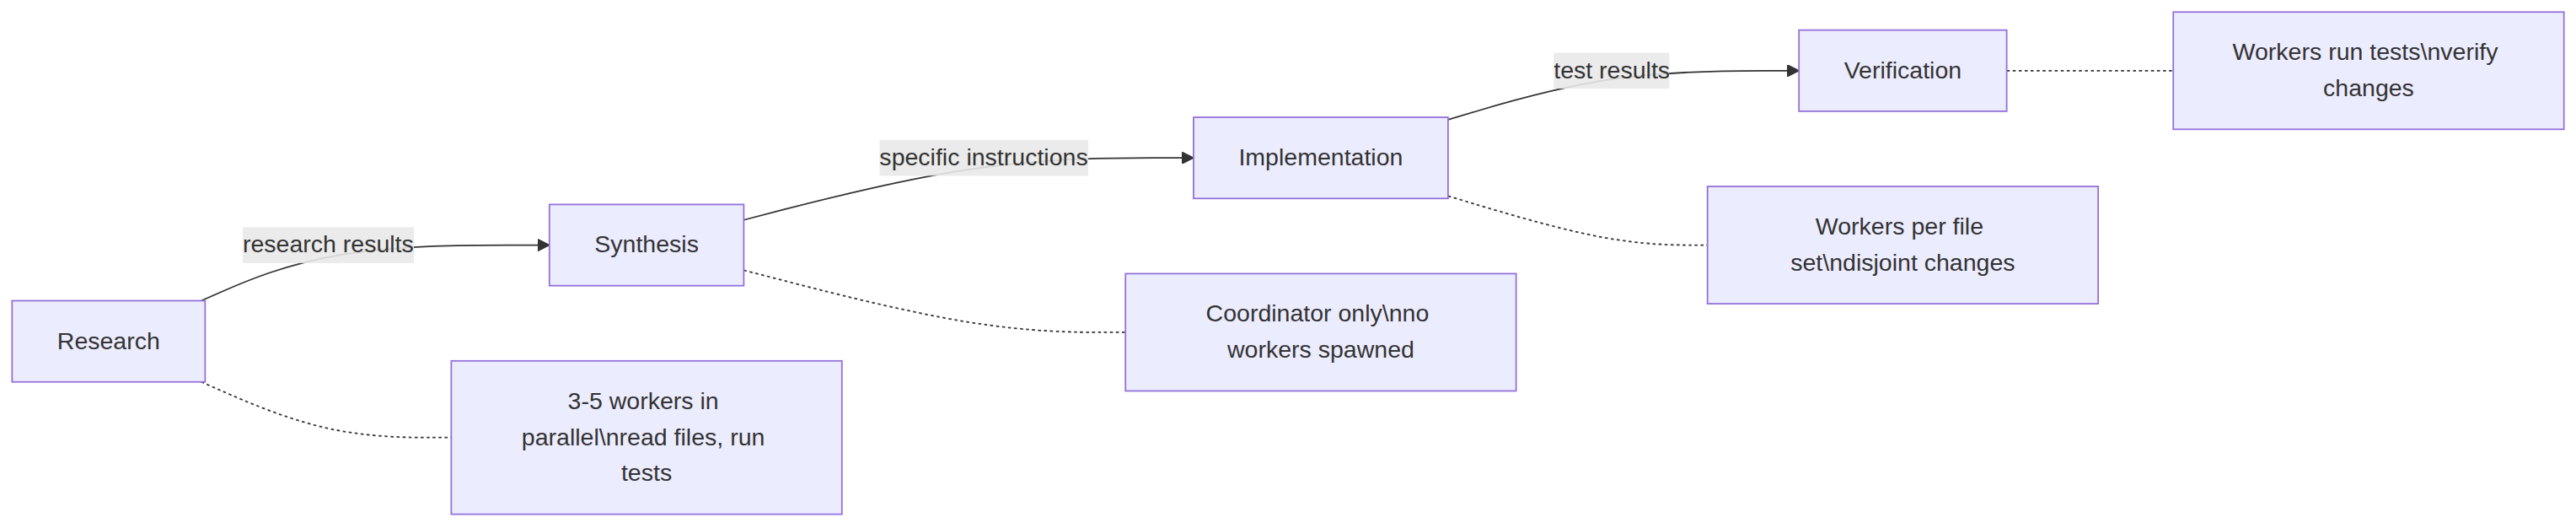
\includegraphics[width=17.86in,height=3.65in]{book/ch10-coordination_files/figure-latex/mermaid-figure-3.png}

\begin{enumerate}
\def\labelenumi{\arabic{enumi}.}
\tightlist
\item
  \textbf{Research} -- workers explore the codebase in parallel, reading
  files, running tests, gathering information
\item
  \textbf{Synthesis} -- the coordinator (not a worker) reads all
  research results and builds a unified understanding
\item
  \textbf{Implementation} -- workers receive precise instructions
  derived from the synthesis
\item
  \textbf{Verification} -- workers run tests and verify the changes
\end{enumerate}

The coordinator should not skip phases. The most common failure mode is
jumping from research directly to implementation without synthesis. When
this happens, the coordinator delegates understanding to the
implementation workers -- each one must re-derive context from scratch,
leading to inconsistent changes and wasted tokens.

\textbf{The continue-vs-spawn decision.} When a worker finishes and the
coordinator has follow-up work, should it send a message to the existing
worker (via SendMessage) or spawn a fresh one (via Agent)? The decision
is a function of context overlap:

\begin{itemize}
\tightlist
\item
  \textbf{High overlap, same files}: Continue. The worker already has
  the file contents in its context, understands the patterns, and can
  build on its previous work. Spawning fresh would force re-reading the
  same files and re-deriving the same understanding.
\item
  \textbf{Low overlap, different domain}: Spawn fresh. A worker that
  just investigated the authentication system carries 20,000 tokens of
  auth-specific context that is dead weight for a CSS refactoring task.
  Starting clean is cheaper.
\item
  \textbf{High overlap but the worker failed}: Spawn fresh with explicit
  guidance about what went wrong. Continuing a failed worker often means
  fighting against confused context. A fresh start with ``the previous
  attempt failed because X, avoid Y'' is more reliable.
\item
  \textbf{Follow-up requires the worker's output}: Continue, with the
  output included in the SendMessage. The worker does not need to
  re-derive its own results.
\end{itemize}

\textbf{Worker prompt writing and anti-patterns.} The prompt teaches the
coordinator how to write effective worker prompts and explicitly flags
bad patterns:

Anti-pattern: \emph{``Based on your research findings, implement the
fix.''} This delegates comprehension. The worker was not the one who did
the research -- the coordinator read the research results.

Anti-pattern: \emph{``Fix the bug in the auth module.''} No file paths,
no line numbers, no description of the bug. The worker must search the
entire codebase from scratch.

Anti-pattern: \emph{``Make the same change to all the other files.''}
Which files? What change? The coordinator knows; it should enumerate
them.

Good pattern: \emph{``In \texttt{src/auth/validate.ts} at line 42, the
\texttt{userId} parameter can be null when called from
\texttt{src/oauth/callback.ts:89}. Add a null check: if \texttt{userId}
is null, return
\texttt{\{\ error:\ \textquotesingle{}unauthorized\textquotesingle{},\ status:\ 401\ \}}.
Then update the test in \texttt{src/auth/\_\_tests\_\_/validate.test.ts}
to cover the null case.''}

The cost of writing a specific prompt is borne once, by the coordinator.
The benefit -- a worker that executes correctly on the first try -- is
enormous. Vague prompts create a false economy: the coordinator saves 30
seconds of prompt writing and the worker wastes 5 minutes of
exploration.

\subsection{Worker Context}\label{worker-context}

The coordinator injects information about available tools into its own
context, so the model knows what workers can do:

\begin{Shaded}
\begin{Highlighting}[]
\ImportTok{export} \KeywordTok{function} \FunctionTok{getCoordinatorUserContext}\NormalTok{(mcpClients}\OperatorTok{,}\NormalTok{ scratchpadDir}\OperatorTok{?}\NormalTok{) \{}
  \ControlFlowTok{return}\NormalTok{ \{}
\NormalTok{    workerToolsContext}\OperatorTok{:} \VerbatimStringTok{\textasciigrave{}Workers spawned via Agent have access to: }\SpecialCharTok{$\{}\NormalTok{workerTools}\SpecialCharTok{\}}\VerbatimStringTok{\textasciigrave{}}
      \OperatorTok{+}\NormalTok{ (mcpClients}\OperatorTok{.}\AttributeTok{length} \OperatorTok{\textgreater{}} \DecValTok{0}
        \OperatorTok{?} \VerbatimStringTok{\textasciigrave{}}\SpecialCharTok{\textbackslash{}n}\VerbatimStringTok{Workers also have MCP tools from: }\SpecialCharTok{$\{}\NormalTok{serverNames}\SpecialCharTok{\}}\VerbatimStringTok{\textasciigrave{}} \OperatorTok{:} \StringTok{\textquotesingle{}\textquotesingle{}}\NormalTok{)}
      \OperatorTok{+}\NormalTok{ (scratchpadDir }\OperatorTok{?} \VerbatimStringTok{\textasciigrave{}}\SpecialCharTok{\textbackslash{}n}\VerbatimStringTok{Scratchpad: }\SpecialCharTok{$\{}\NormalTok{scratchpadDir}\SpecialCharTok{\}}\VerbatimStringTok{\textasciigrave{}} \OperatorTok{:} \StringTok{\textquotesingle{}\textquotesingle{}}\NormalTok{)}
\NormalTok{  \}}
\NormalTok{\}}
\end{Highlighting}
\end{Shaded}

The scratchpad directory (gated by the \texttt{tengu\_scratch} feature
flag) is a shared filesystem location where workers can read and write
without permission prompts. It enables durable cross-worker knowledge
sharing -- one worker's research notes become another worker's input,
mediated through the filesystem rather than through the coordinator's
token window.

This is significant because it solves a fundamental limitation of the
coordinator pattern. Without a scratchpad, all information flows through
the coordinator: Worker A produces findings, the coordinator reads them
via TaskOutput, synthesizes them into Worker B's prompt. The
coordinator's context window becomes the bottleneck -- it must hold all
intermediate results long enough to synthesize them. With a scratchpad,
Worker A writes findings to \texttt{/tmp/scratchpad/auth-analysis.md},
and the coordinator tells Worker B: ``Read the auth analysis at
\texttt{/tmp/scratchpad/auth-analysis.md} and apply the pattern to the
OAuth module.'' The coordinator moves information by reference, not by
value.

\subsection{Mutual Exclusion with
Fork}\label{mutual-exclusion-with-fork}

Coordinator mode and fork-based subagents are mutually exclusive:

\begin{Shaded}
\begin{Highlighting}[]
\ImportTok{export} \KeywordTok{function} \FunctionTok{isForkSubagentEnabled}\NormalTok{()}\OperatorTok{:} \DataTypeTok{boolean}\NormalTok{ \{}
  \ControlFlowTok{if}\NormalTok{ (}\FunctionTok{feature}\NormalTok{(}\StringTok{\textquotesingle{}FORK\_SUBAGENT\textquotesingle{}}\NormalTok{)) \{}
    \ControlFlowTok{if}\NormalTok{ (}\FunctionTok{isCoordinatorMode}\NormalTok{()) }\ControlFlowTok{return} \KeywordTok{false}
    \CommentTok{// ...}
\NormalTok{  \}}
\NormalTok{\}}
\end{Highlighting}
\end{Shaded}

The conflict is fundamental. Fork agents inherit the parent's entire
conversation context -- they are cheap clones that share prompt cache.
Coordinator workers are independent agents with fresh context and
specific instructions. These are opposing philosophies of delegation,
and the system enforces the choice at the feature flag level.

\begin{center}\rule{0.5\linewidth}{0.5pt}\end{center}

\section{The Swarm System}\label{the-swarm-system}

Coordinator mode is hierarchical: one manager, many workers, top-down
control. The swarm system is the peer-to-peer alternative -- multiple
Claude Code instances working as a team, with a leader coordinating
multiple teammates through message passing.

\subsection{Team Context}\label{team-context}

Teams are identified by a \texttt{teamName} and tracked in
\texttt{AppState.teamContext}:

\begin{Shaded}
\begin{Highlighting}[]
\NormalTok{teamContext}\OperatorTok{?:}\NormalTok{ \{}
\NormalTok{  teamName}\OperatorTok{:} \DataTypeTok{string}
\NormalTok{  teammates}\OperatorTok{:}\NormalTok{ \{}
\NormalTok{    [id}\OperatorTok{:} \DataTypeTok{string}\NormalTok{]}\OperatorTok{:}\NormalTok{ \{ name}\OperatorTok{:} \DataTypeTok{string}\OperatorTok{;}\NormalTok{ color}\OperatorTok{?:} \DataTypeTok{string}\OperatorTok{;} \OperatorTok{...}\NormalTok{ \}}
\NormalTok{  \}}
\NormalTok{\}}
\end{Highlighting}
\end{Shaded}

Each teammate gets a name (for addressing) and a color (for visual
distinction in the UI). The team file is persisted on disk so that team
membership survives process restarts.

\subsection{Agent Name Registry}\label{agent-name-registry}

Background agents can be given names at spawn time, which makes them
addressable by human-readable identifiers instead of random task IDs:

\begin{Shaded}
\begin{Highlighting}[]
\ControlFlowTok{if}\NormalTok{ (name) \{}
  \FunctionTok{rootSetAppState}\NormalTok{(prev }\KeywordTok{=\textgreater{}}\NormalTok{ \{}
    \KeywordTok{const}\NormalTok{ next }\OperatorTok{=} \KeywordTok{new} \BuiltInTok{Map}\NormalTok{(prev}\OperatorTok{.}\AttributeTok{agentNameRegistry}\NormalTok{)}
\NormalTok{    next}\OperatorTok{.}\FunctionTok{set}\NormalTok{(name}\OperatorTok{,} \FunctionTok{asAgentId}\NormalTok{(asyncAgentId))}
    \ControlFlowTok{return}\NormalTok{ \{ }\OperatorTok{...}\NormalTok{prev}\OperatorTok{,}\NormalTok{ agentNameRegistry}\OperatorTok{:}\NormalTok{ next \}}
\NormalTok{  \})}
\NormalTok{\}}
\end{Highlighting}
\end{Shaded}

The \texttt{agentNameRegistry} is a
\texttt{Map\textless{}string,\ AgentId\textgreater{}}. When
\texttt{SendMessage} resolves a \texttt{to} field, the registry is
checked first:

\begin{Shaded}
\begin{Highlighting}[]
\KeywordTok{const}\NormalTok{ registered }\OperatorTok{=}\NormalTok{ appState}\OperatorTok{.}\AttributeTok{agentNameRegistry}\OperatorTok{.}\FunctionTok{get}\NormalTok{(input}\OperatorTok{.}\AttributeTok{to}\NormalTok{)}
\KeywordTok{const}\NormalTok{ agentId }\OperatorTok{=}\NormalTok{ registered }\OperatorTok{??} \FunctionTok{toAgentId}\NormalTok{(input}\OperatorTok{.}\AttributeTok{to}\NormalTok{)}
\end{Highlighting}
\end{Shaded}

This means you can send a message to \texttt{"researcher"} instead of
\texttt{a7j3n9p2}. The indirection is simple but it enables the
coordinator to think in terms of roles rather than IDs -- a significant
improvement for the model's ability to reason about multi-agent
workflows.

\subsection{In-Process Teammates}\label{in-process-teammates}

In-process teammates run in the same Node.js process as the leader,
isolated via \texttt{AsyncLocalStorage}. Their state extends the base
with team-specific fields:

\begin{Shaded}
\begin{Highlighting}[]
\ImportTok{export type}\NormalTok{ InProcessTeammateTaskState }\OperatorTok{=}\NormalTok{ TaskStateBase }\OperatorTok{\&}\NormalTok{ \{}
\NormalTok{  type}\OperatorTok{:} \StringTok{\textquotesingle{}in\_process\_teammate\textquotesingle{}}
\NormalTok{  identity}\OperatorTok{:}\NormalTok{ TeammateIdentity}
\NormalTok{  prompt}\OperatorTok{:} \DataTypeTok{string}
\NormalTok{  messages}\OperatorTok{?:}\NormalTok{ Message[]                  }\CommentTok{// Capped at 50}
\NormalTok{  pendingUserMessages}\OperatorTok{:} \DataTypeTok{string}\NormalTok{[]}
\NormalTok{  isIdle}\OperatorTok{:} \DataTypeTok{boolean}
\NormalTok{  shutdownRequested}\OperatorTok{:} \DataTypeTok{boolean}
\NormalTok{  awaitingPlanApproval}\OperatorTok{:} \DataTypeTok{boolean}
\NormalTok{  permissionMode}\OperatorTok{:}\NormalTok{ PermissionMode}
\NormalTok{  onIdleCallbacks}\OperatorTok{?:} \BuiltInTok{Array}\OperatorTok{\textless{}}\NormalTok{() }\KeywordTok{=\textgreater{}} \DataTypeTok{void}\OperatorTok{\textgreater{}}
\NormalTok{  currentWorkAbortController}\OperatorTok{?:}\NormalTok{ AbortController}
\NormalTok{\}}
\end{Highlighting}
\end{Shaded}

The \texttt{messages} cap at 50 entries deserves explanation. During
development, analysis revealed that each in-process agent accumulates
approximately 20MB of RSS at 500+ turns. Whale sessions -- power users
running extended workflows -- were observed launching 292 agents in 2
minutes, driving RSS to 36.8GB. The 50-message cap for the UI
representation is a memory safety valve. The agent's actual conversation
continues with full history; only the UI-facing snapshot is truncated.

The \texttt{isIdle} flag enables a work-stealing pattern. An idle
teammate is not consuming tokens or API calls -- it is simply waiting
for the next message. The \texttt{onIdleCallbacks} array lets the system
hook into the transition from active to idle, enabling orchestration
patterns like ``wait for all teammates to finish, then proceed.''

The \texttt{currentWorkAbortController} is distinct from the teammate's
main abort controller. Aborting the current work controller cancels the
teammate's ongoing turn but does not kill the teammate. This enables a
``redirect'' pattern: the leader sends a higher-priority message, the
teammate's current work is aborted, and the teammate picks up the new
message. The main abort controller, when aborted, kills the teammate
entirely. Two levels of interruption for two levels of intent.

The \texttt{shutdownRequested} flag implements cooperative termination.
When the leader sends a shutdown request, this flag is set. The teammate
can check it at natural stopping points and wind down gracefully --
finishing its current file write, committing its changes, or sending a
final status update. This is gentler than a hard kill, which might leave
files in an inconsistent state.

\subsection{The Mailbox}\label{the-mailbox}

Teammates communicate via a file-based mailbox system. When
\texttt{SendMessage} targets a teammate, the message is written to the
recipient's mailbox file on disk:

\begin{Shaded}
\begin{Highlighting}[]
\ControlFlowTok{await} \FunctionTok{writeToMailbox}\NormalTok{(recipientName}\OperatorTok{,}\NormalTok{ \{}
\NormalTok{  from}\OperatorTok{:}\NormalTok{ senderName}\OperatorTok{,}
\NormalTok{  text}\OperatorTok{:}\NormalTok{ content}\OperatorTok{,}
\NormalTok{  summary}\OperatorTok{,}
\NormalTok{  timestamp}\OperatorTok{:} \KeywordTok{new} \BuiltInTok{Date}\NormalTok{()}\OperatorTok{.}\FunctionTok{toISOString}\NormalTok{()}\OperatorTok{,}
\NormalTok{  color}\OperatorTok{:}\NormalTok{ senderColor}\OperatorTok{,}
\NormalTok{\}}\OperatorTok{,}\NormalTok{ teamName)}
\end{Highlighting}
\end{Shaded}

Messages can be plain text, structured protocol messages (shutdown
requests, plan approvals), or broadcasts (\texttt{to:\ "*"} sends to all
team members excluding the sender). A poller hook processes incoming
messages and routes them into the teammate's conversation.

The file-based approach is deliberately simple. There is no message
broker, no event bus, no shared memory channel. Files are durable
(surviving process crashes), inspectable (you can \texttt{cat} a
mailbox), and cheap (no infrastructure dependencies). For a system where
message volumes are measured in tens per session, not thousands per
second, this is the right trade-off. A Redis-backed message queue would
add operational complexity, a dependency, and failure modes -- all for a
throughput requirement that a filesystem call handles trivially.

The broadcast mechanism deserves a note. When a message is sent to
\texttt{"*"}, the sender iterates all team members from the team file,
skips itself (case-insensitive comparison), and writes to each member's
mailbox individually:

\begin{Shaded}
\begin{Highlighting}[]
\ControlFlowTok{for}\NormalTok{ (}\KeywordTok{const}\NormalTok{ member }\KeywordTok{of}\NormalTok{ teamFile}\OperatorTok{.}\AttributeTok{members}\NormalTok{) \{}
  \ControlFlowTok{if}\NormalTok{ (member}\OperatorTok{.}\AttributeTok{name}\OperatorTok{.}\FunctionTok{toLowerCase}\NormalTok{() }\OperatorTok{===}\NormalTok{ senderName}\OperatorTok{.}\FunctionTok{toLowerCase}\NormalTok{()) }\ControlFlowTok{continue}
\NormalTok{  recipients}\OperatorTok{.}\FunctionTok{push}\NormalTok{(member}\OperatorTok{.}\AttributeTok{name}\NormalTok{)}
\NormalTok{\}}
\ControlFlowTok{for}\NormalTok{ (}\KeywordTok{const}\NormalTok{ recipientName }\KeywordTok{of}\NormalTok{ recipients) \{}
  \ControlFlowTok{await} \FunctionTok{writeToMailbox}\NormalTok{(recipientName}\OperatorTok{,}\NormalTok{ \{ from}\OperatorTok{:}\NormalTok{ senderName}\OperatorTok{,}\NormalTok{ text}\OperatorTok{:}\NormalTok{ content}\OperatorTok{,} \OperatorTok{...}\NormalTok{ \}}\OperatorTok{,}\NormalTok{ teamName)}
\NormalTok{\}}
\end{Highlighting}
\end{Shaded}

There is no fan-out optimization -- each recipient gets a separate file
write. Again, at the scale of agent teams (typically 3-8 members), this
is perfectly adequate. If a team had 100 members, this would need
rethinking. But the 50-message memory cap that prevents 36GB RSS
scenarios also implicitly caps the effective team size.

\subsection{Permission Forwarding}\label{permission-forwarding}

Swarm workers operate with restricted permissions but can escalate to
the leader when they need approval for sensitive operations:

\begin{Shaded}
\begin{Highlighting}[]
\KeywordTok{const}\NormalTok{ request }\OperatorTok{=} \FunctionTok{createPermissionRequest}\NormalTok{(\{}
\NormalTok{  toolName}\OperatorTok{,}\NormalTok{ toolUseId}\OperatorTok{,}\NormalTok{ input}\OperatorTok{,}\NormalTok{ description}\OperatorTok{,}\NormalTok{ permissionSuggestions}
\NormalTok{\})}
\FunctionTok{registerPermissionCallback}\NormalTok{(\{ requestId}\OperatorTok{,}\NormalTok{ toolUseId}\OperatorTok{,}\NormalTok{ onAllow}\OperatorTok{,}\NormalTok{ onReject \})}
\KeywordTok{void} \FunctionTok{sendPermissionRequestViaMailbox}\NormalTok{(request)}
\end{Highlighting}
\end{Shaded}

The flow is: worker hits a tool that requires permission, the bash
classifier attempts auto-approval, and if that fails, the request is
forwarded to the leader via the mailbox system. The leader sees the
request in their UI and can approve or reject. The callback fires and
the worker proceeds. This lets workers operate autonomously for safe
operations while maintaining human oversight for dangerous ones.

\begin{center}\rule{0.5\linewidth}{0.5pt}\end{center}

\section{Inter-Agent Communication:
SendMessage}\label{inter-agent-communication-sendmessage}

\texttt{SendMessageTool} is the universal communication primitive. It
handles four distinct routing modes through a single tool interface,
selected by the shape of the \texttt{to} field.

\subsection{Input Schema}\label{input-schema}

\begin{Shaded}
\begin{Highlighting}[]
\NormalTok{inputSchema }\OperatorTok{=}\NormalTok{ z}\OperatorTok{.}\FunctionTok{object}\NormalTok{(\{}
\NormalTok{  to}\OperatorTok{:}\NormalTok{ z}\OperatorTok{.}\FunctionTok{string}\NormalTok{()}\OperatorTok{,}
  \CommentTok{// "teammate{-}name", "*", "uds:\textless{}socket\textgreater{}", "bridge:\textless{}session{-}id\textgreater{}"}
\NormalTok{  summary}\OperatorTok{:}\NormalTok{ z}\OperatorTok{.}\FunctionTok{string}\NormalTok{()}\OperatorTok{.}\FunctionTok{optional}\NormalTok{()}\OperatorTok{,}
\NormalTok{  message}\OperatorTok{:}\NormalTok{ z}\OperatorTok{.}\FunctionTok{union}\NormalTok{([}
\NormalTok{    z}\OperatorTok{.}\FunctionTok{string}\NormalTok{()}\OperatorTok{,}
\NormalTok{    z}\OperatorTok{.}\FunctionTok{discriminatedUnion}\NormalTok{(}\StringTok{\textquotesingle{}type\textquotesingle{}}\OperatorTok{,}\NormalTok{ [}
\NormalTok{      z}\OperatorTok{.}\FunctionTok{object}\NormalTok{(\{ type}\OperatorTok{:}\NormalTok{ z}\OperatorTok{.}\FunctionTok{literal}\NormalTok{(}\StringTok{\textquotesingle{}shutdown\_request\textquotesingle{}}\NormalTok{)}\OperatorTok{,}\NormalTok{ reason}\OperatorTok{:}\NormalTok{ z}\OperatorTok{.}\FunctionTok{string}\NormalTok{()}\OperatorTok{.}\FunctionTok{optional}\NormalTok{() \})}\OperatorTok{,}
\NormalTok{      z}\OperatorTok{.}\FunctionTok{object}\NormalTok{(\{ type}\OperatorTok{:}\NormalTok{ z}\OperatorTok{.}\FunctionTok{literal}\NormalTok{(}\StringTok{\textquotesingle{}shutdown\_response\textquotesingle{}}\NormalTok{)}\OperatorTok{,}\NormalTok{ request\_id}\OperatorTok{,}\NormalTok{ approve}\OperatorTok{,}\NormalTok{ reason \})}\OperatorTok{,}
\NormalTok{      z}\OperatorTok{.}\FunctionTok{object}\NormalTok{(\{ type}\OperatorTok{:}\NormalTok{ z}\OperatorTok{.}\FunctionTok{literal}\NormalTok{(}\StringTok{\textquotesingle{}plan\_approval\_response\textquotesingle{}}\NormalTok{)}\OperatorTok{,}\NormalTok{ request\_id}\OperatorTok{,}\NormalTok{ approve}\OperatorTok{,}\NormalTok{ feedback \})}\OperatorTok{,}
\NormalTok{    ])}\OperatorTok{,}
\NormalTok{  ])}\OperatorTok{,}
\NormalTok{\})}
\end{Highlighting}
\end{Shaded}

The \texttt{message} field is a union of plain text and structured
protocol messages. This means SendMessage serves double duty -- it is
both the informal chat channel (``here are my findings'') and the formal
protocol layer (``I approve your plan'' / ``please shut down'').

\subsection{Routing Dispatch}\label{routing-dispatch}

The \texttt{call()} method follows a priority-ordered dispatch chain:

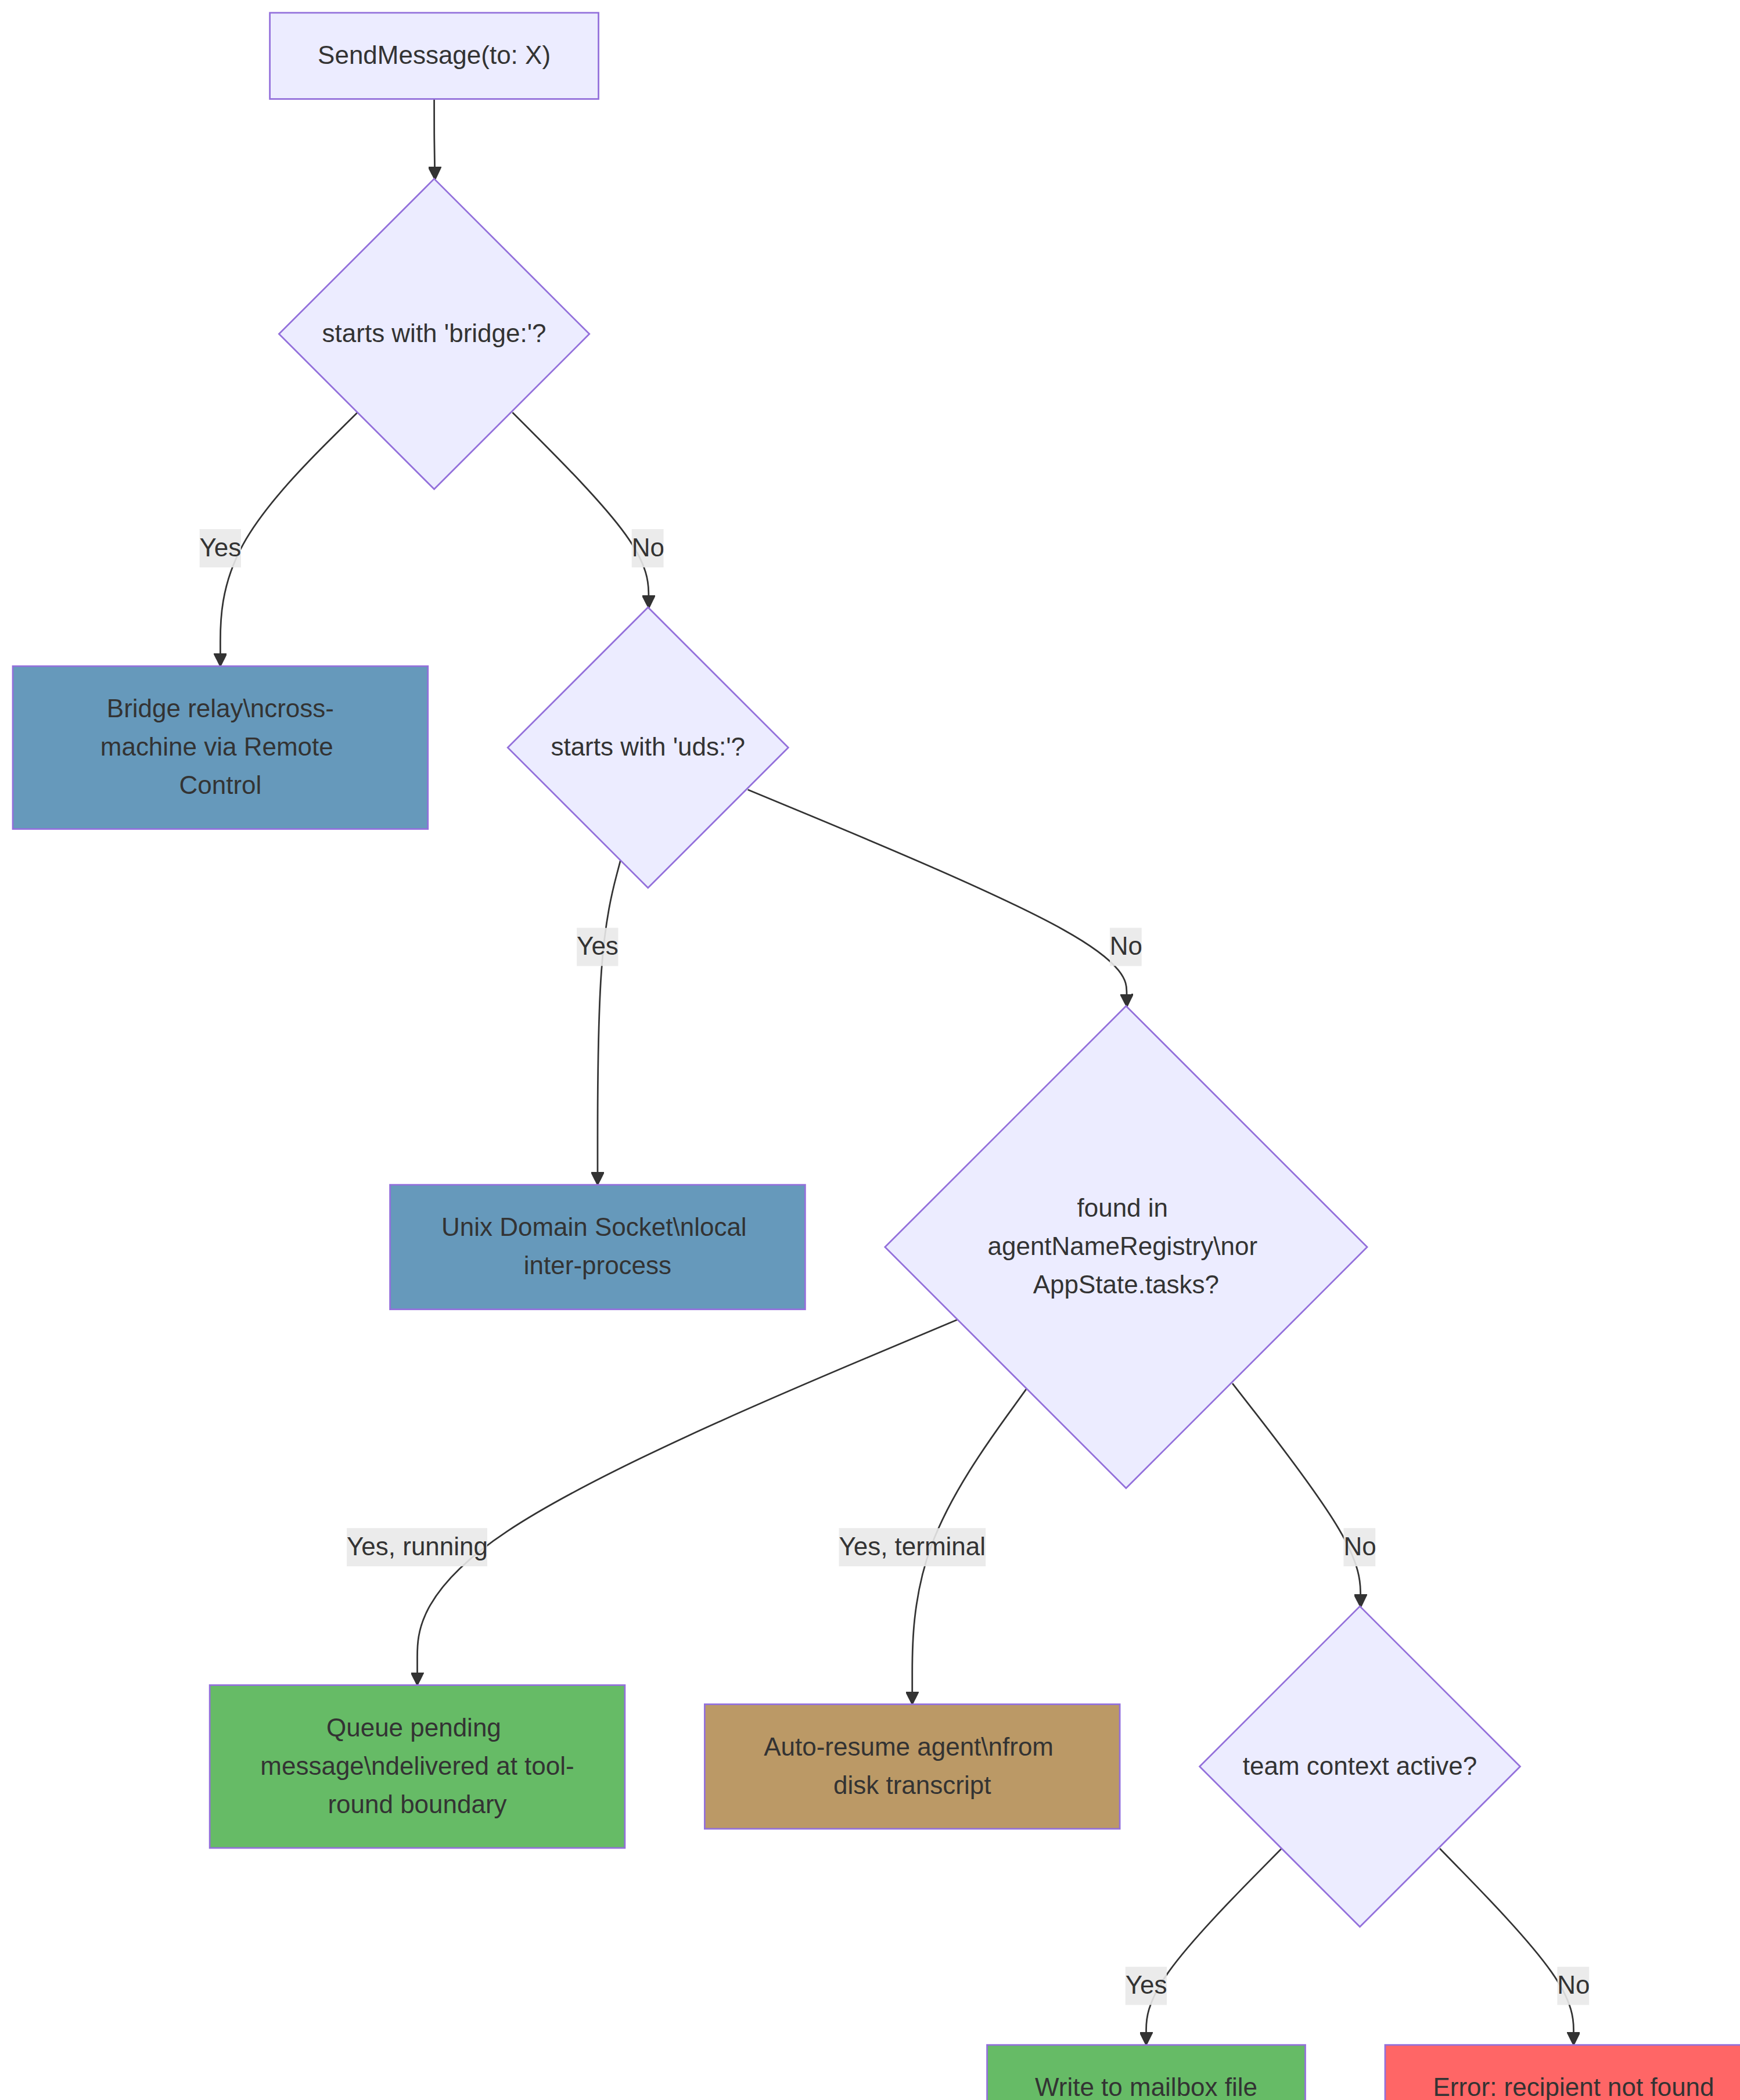
\includegraphics[width=11.58in,height=13.99in]{book/ch10-coordination_files/figure-latex/mermaid-figure-2.png}

\textbf{1. Bridge messages}
(\texttt{bridge:\textless{}session-id\textgreater{}}). Cross-machine
communication via Anthropic's Remote Control servers. This is the widest
reach -- two Claude Code instances on different machines, potentially
different continents, communicating through a relay. The system requires
explicit user consent before sending bridge messages -- a safety check
that prevents one agent from unilaterally establishing communication
with a remote instance. Without this gate, a compromised or confused
agent could exfiltrate information to a remote session. The consent
check uses \texttt{postInterClaudeMessage()}, which handles
serialization and transport over the Remote Control relay.

\textbf{2. UDS messages}
(\texttt{uds:\textless{}socket-path\textgreater{}}). Local inter-process
communication via Unix Domain Sockets. This is for Claude Code instances
running on the same machine but in different processes -- for example, a
VS Code extension hosting one instance and a terminal hosting another.
UDS communication is fast (no network round-trip), secure (filesystem
permissions control access), and reliable (the kernel handles delivery).
The \texttt{sendToUdsSocket()} function serializes the message and
writes it to the socket path specified in the \texttt{to} field. Peers
discover each other via a \texttt{ListPeers} tool that scans for active
UDS endpoints.

\textbf{3. In-process subagent routing} (plain name or agent ID). This
is the most common path. The routing logic:

\begin{itemize}
\tightlist
\item
  Look up \texttt{input.to} in the \texttt{agentNameRegistry}
\item
  If found and running: \texttt{queuePendingMessage()} -- the message
  waits for the next tool-round boundary
\item
  If found but in a terminal state: \texttt{resumeAgentBackground()} --
  the agent is transparently restarted
\item
  If not in \texttt{AppState}: attempt to resume from the disk
  transcript
\end{itemize}

\textbf{4. Team mailbox} (fallback when team context is active). Named
recipients get messages written to their mailbox files. The \texttt{"*"}
wildcard triggers a broadcast to all team members.

\subsection{Structured Protocols}\label{structured-protocols}

Beyond plain text, SendMessage carries two formal protocols.

\textbf{The shutdown protocol.} The leader sends
\texttt{\{\ type:\ \textquotesingle{}shutdown\_request\textquotesingle{},\ reason:\ \textquotesingle{}...\textquotesingle{}\ \}}
to a teammate. The teammate responds with
\texttt{\{\ type:\ \textquotesingle{}shutdown\_response\textquotesingle{},\ request\_id,\ approve:\ true/false,\ reason\ \}}.
If approved, in-process teammates abort their controller; tmux-based
teammates receive a \texttt{gracefulShutdown()} call. The protocol is
cooperative -- a teammate can reject a shutdown request if it is in the
middle of critical work, and the leader must handle that case.

\textbf{The plan approval protocol.} Teammates operating in plan mode
must get approval before executing. They submit a plan, and the leader
responds with
\texttt{\{\ type:\ \textquotesingle{}plan\_approval\_response\textquotesingle{},\ request\_id,\ approve,\ feedback\ \}}.
Only the team lead can issue approvals. This creates a review gate --
the leader can examine a worker's intended approach before any files are
touched, catching misunderstandings early.

\subsection{The Auto-Resume Pattern}\label{the-auto-resume-pattern}

The most elegant feature of the routing system is transparent agent
resumption. When \texttt{SendMessage} targets a completed or killed
agent, instead of returning an error, it resurrects the agent:

\begin{Shaded}
\begin{Highlighting}[]
\ControlFlowTok{if}\NormalTok{ (task}\OperatorTok{.}\AttributeTok{status} \OperatorTok{!==} \StringTok{\textquotesingle{}running\textquotesingle{}}\NormalTok{) \{}
  \KeywordTok{const}\NormalTok{ result }\OperatorTok{=} \ControlFlowTok{await} \FunctionTok{resumeAgentBackground}\NormalTok{(\{}
\NormalTok{    agentId}\OperatorTok{,}
\NormalTok{    prompt}\OperatorTok{:}\NormalTok{ input}\OperatorTok{.}\AttributeTok{message}\OperatorTok{,}
\NormalTok{    toolUseContext}\OperatorTok{:}\NormalTok{ context}\OperatorTok{,}
\NormalTok{    canUseTool}\OperatorTok{,}
\NormalTok{  \})}
  \ControlFlowTok{return}\NormalTok{ \{}
\NormalTok{    data}\OperatorTok{:}\NormalTok{ \{}
\NormalTok{      success}\OperatorTok{:} \KeywordTok{true}\OperatorTok{,}
\NormalTok{      message}\OperatorTok{:} \VerbatimStringTok{\textasciigrave{}Agent "}\SpecialCharTok{$\{}\NormalTok{input}\OperatorTok{.}\AttributeTok{to}\SpecialCharTok{\}}\VerbatimStringTok{" was stopped; resumed with your message\textasciigrave{}}
\NormalTok{    \}}
\NormalTok{  \}}
\NormalTok{\}}
\end{Highlighting}
\end{Shaded}

The \texttt{resumeAgentBackground()} function reconstructs the agent
from its disk transcript:

\begin{enumerate}
\def\labelenumi{\arabic{enumi}.}
\tightlist
\item
  Reads the sidechain JSONL transcript
\item
  Reconstructs the message history, filtering orphaned thinking blocks
  and unresolved tool uses
\item
  Rebuilds the content replacement state for prompt cache stability
\item
  Resolves the original agent definition from stored metadata
\item
  Re-registers as a background task with a fresh abort controller
\item
  Calls \texttt{runAgent()} with the restored history plus the new
  message as prompt
\end{enumerate}

From the coordinator's perspective, sending a message to a dead agent
and sending a message to a live agent are the same operation. The
routing layer handles the complexity. This means coordinators do not
need to track which agents are alive -- they simply send messages and
the system figures it out.

The implications are significant. Without auto-resume, the coordinator
would need to maintain a mental model of agent liveness: ``Is
\texttt{researcher} still running? Let me check. It completed. I need to
spawn a new agent. But wait, should I use the same name? Will it have
the same context?'' With auto-resume, all of that collapses to: ``Send
\texttt{researcher} a message.'' If it is alive, the message is queued.
If it is dead, it is resurrected with its full history. The
coordinator's prompt complexity drops dramatically.

There is a cost, of course. Resuming from a disk transcript means
re-reading potentially thousands of messages, reconstructing internal
state, and making a new API call with a full context window. For a
long-lived agent, this can be expensive in both latency and tokens. But
the alternative -- requiring the coordinator to manually manage agent
lifecycles -- is worse. The coordinator is an LLM. It is good at
reasoning about problems and writing instructions. It is bad at
bookkeeping. Auto-resume plays to the LLM's strengths by eliminating a
category of bookkeeping entirely.

\begin{center}\rule{0.5\linewidth}{0.5pt}\end{center}

\section{TaskStop: The Kill Switch}\label{taskstop-the-kill-switch}

\texttt{TaskStopTool} is the complement to Agent and SendMessage -- it
terminates running tasks:

\begin{Shaded}
\begin{Highlighting}[]
\NormalTok{inputSchema }\OperatorTok{=}\NormalTok{ z}\OperatorTok{.}\FunctionTok{strictObject}\NormalTok{(\{}
\NormalTok{  task\_id}\OperatorTok{:}\NormalTok{ z}\OperatorTok{.}\FunctionTok{string}\NormalTok{()}\OperatorTok{.}\FunctionTok{optional}\NormalTok{()}\OperatorTok{,}
\NormalTok{  shell\_id}\OperatorTok{:}\NormalTok{ z}\OperatorTok{.}\FunctionTok{string}\NormalTok{()}\OperatorTok{.}\FunctionTok{optional}\NormalTok{()}\OperatorTok{,}  \CommentTok{// Deprecated backward compat}
\NormalTok{\})}
\end{Highlighting}
\end{Shaded}

The implementation delegates to \texttt{stopTask()}, which dispatches
based on task type:

\begin{enumerate}
\def\labelenumi{\arabic{enumi}.}
\tightlist
\item
  Look up the task in \texttt{AppState.tasks}
\item
  Call \texttt{getTaskByType(task.type).kill(taskId,\ setAppState)}
\item
  For agents: abort the controller, set status to
  \texttt{\textquotesingle{}killed\textquotesingle{}}, start the
  eviction timer
\item
  For shells: kill the process group
\end{enumerate}

The tool has a legacy alias \texttt{"KillShell"} -- a reminder that the
task system evolved from simpler origins where the only background
operation was a shell command.

The kill mechanism varies by task type, but the pattern is consistent.
For agents, killing means aborting the abort controller (which causes
the \texttt{query()} loop to exit at the next yield point), setting the
status to \texttt{\textquotesingle{}killed\textquotesingle{}}, and
starting an eviction timer so the task state is cleaned up after a grace
period. For shells, killing means sending a signal to the process group
-- \texttt{SIGTERM} first, then \texttt{SIGKILL} if the process does not
exit within a timeout. For in-process teammates, killing also triggers a
shutdown notification to the team so other members know the teammate is
gone.

The eviction timer is worth noting. When an agent is killed, its state
is not immediately purged. It lingers in \texttt{AppState.tasks} for a
grace period (controlled by \texttt{evictAfter}) so that the UI can show
the killed status, any final output can be read, and auto-resume via
SendMessage remains possible. After the grace period, the state is
garbage collected. This is the same pattern used for completed tasks --
the system distinguishes between ``finished'' (result available) and
``forgotten'' (state purged).

\begin{center}\rule{0.5\linewidth}{0.5pt}\end{center}

\section{Choosing Between Patterns}\label{choosing-between-patterns}

(A note on naming: the codebase also contains
\texttt{TaskCreate}/\texttt{TaskGet}/\texttt{TaskList}/\texttt{TaskUpdate}
tools that manage a structured todo list -- a completely separate system
from the background task state machine described here. \texttt{TaskStop}
operates on \texttt{AppState.tasks}; \texttt{TaskUpdate} operates on a
project tracking data store. The naming overlap is historical and a
recurring source of model confusion.)

With three orchestration patterns available -- background delegation,
coordinator mode, and swarm teams -- the natural question is when to use
each.

\textbf{Simple delegation} (Agent tool with
\texttt{run\_in\_background:\ true}) is appropriate when the parent has
one or two independent tasks to offload. Run the tests in the background
while continuing to edit. Search the codebase while waiting for a build.
The parent stays in control, checks results when ready, and never needs
a complex communication protocol. The overhead is minimal -- one task
state entry, one disk output file, one notification on completion.

\textbf{Coordinator mode} is appropriate when the problem decomposes
into a research phase, a synthesis phase, and an implementation phase --
and when the coordinator needs to reason across the results of multiple
workers before directing the next step. The coordinator cannot touch
files, which forces clean separation of concerns: thinking happens in
one context, doing happens in another. The 370-line system prompt is not
ceremony -- it encodes patterns that prevent the most common failure
mode of LLM delegation, which is delegating comprehension instead of
delegating action.

\textbf{Swarm teams} are appropriate for long-running collaborative
sessions where agents need peer-to-peer communication, where the work is
ongoing rather than batch-oriented, and where agents may need to idle
and resume based on incoming messages. The mailbox system supports
asynchronous patterns that coordinator mode (which is synchronous
spawn-wait-synthesize) does not. Plan approval gates add a review layer.
Permission forwarding maintains security without requiring every agent
to have full privileges.

A practical decision table:

\begin{longtable}[]{@{}
  >{\raggedright\arraybackslash}p{(\linewidth - 4\tabcolsep) * \real{0.4167}}
  >{\raggedright\arraybackslash}p{(\linewidth - 4\tabcolsep) * \real{0.3750}}
  >{\raggedright\arraybackslash}p{(\linewidth - 4\tabcolsep) * \real{0.2083}}@{}}
\toprule\noalign{}
\begin{minipage}[b]{\linewidth}\raggedright
Scenario
\end{minipage} & \begin{minipage}[b]{\linewidth}\raggedright
Pattern
\end{minipage} & \begin{minipage}[b]{\linewidth}\raggedright
Why
\end{minipage} \\
\midrule\noalign{}
\endhead
\bottomrule\noalign{}
\endlastfoot
Run tests while editing & Simple delegation & One background task, no
coordination needed \\
Search codebase for all usages & Simple delegation & Fire-and-forget,
read output when done \\
Refactor 40 files across 3 modules & Coordinator & Research phase finds
patterns, synthesis plans changes, workers execute in parallel per
module \\
Multi-day feature development with review gates & Swarm & Long-lived
agents, plan approval protocol, peer communication \\
Fix a bug with known location & Neither -- single agent & Orchestration
overhead exceeds the benefit for focused, sequential work \\
Migrate database schema + update API + update frontend & Coordinator &
Three independent workstreams after a shared research/planning phase \\
Pair programming with user oversight & Swarm with plan mode & Worker
proposes, leader approves, worker executes \\
\end{longtable}

The patterns are not mutually exclusive in principle, but they are in
practice. Coordinator mode disables fork subagents. Swarm teams have
their own communication protocol that does not mix with coordinator task
notifications. The choice is made at session startup via environment
variables and feature flags, and it shapes the entire interaction model.

One final observation: the simplest pattern is almost always the right
starting point. Most tasks do not need coordinator mode or swarm teams.
A single agent with occasional background delegation handles the vast
majority of development work. The sophisticated patterns exist for the
5\% of cases where the problem is genuinely wide, genuinely parallel, or
genuinely long-running. Reaching for coordinator mode on a single-file
bug fix is like deploying Kubernetes for a static website -- technically
possible, architecturally inappropriate.

\begin{center}\rule{0.5\linewidth}{0.5pt}\end{center}

\section{The Cost of Orchestration}\label{the-cost-of-orchestration}

Before examining what the orchestration layer reveals philosophically,
it is worth acknowledging what it costs practically.

Every background agent is a separate API conversation. It has its own
context window, its own token budget, and its own prompt cache slot. A
coordinator that spawns 5 research workers is making 6 concurrent API
calls, each with its own system prompt, tool definitions, and CLAUDE.md
injection. The token overhead is not trivial -- the system prompt alone
can be thousands of tokens, and each worker re-reads files that other
workers may have already read.

The communication channels add latency. Disk output files require
filesystem I/O. Task notifications are delivered at tool-round
boundaries, not instantly. The command queue introduces a full
round-trip delay -- the coordinator sends a message, the message waits
for the worker to finish its current tool use, the worker processes the
message, and the result is written to disk for the coordinator to read.

The state management adds complexity. Seven task types, five statuses,
and dozens of fields per task state. The eviction logic, the garbage
collection timers, the memory caps -- all of this exists because
unbounded state growth caused real production incidents (36.8GB RSS).

None of this means orchestration is wrong. It means orchestration is a
tool with a cost, and the cost should be weighed against the benefit.
Running 5 parallel workers to search a codebase is worthwhile when the
search would take 5 sequential minutes. Running a coordinator to fix a
typo in one file is pure overhead.

\begin{center}\rule{0.5\linewidth}{0.5pt}\end{center}

\section{What the Orchestration Layer
Reveals}\label{what-the-orchestration-layer-reveals}

The most interesting aspect of this system is not any individual
mechanism -- task states, mailboxes, and notification XML are all
straightforward engineering. What is interesting is the \emph{design
philosophy} that emerges from how they fit together.

The coordinator prompt's ``never delegate understanding'' is not just
good advice for LLM orchestration. It is a statement about the
fundamental limitation of context-window-based reasoning. A worker with
a fresh context window cannot understand what the coordinator understood
after reading 50 files and synthesizing three research reports. The only
way to bridge that gap is for the coordinator to distill its
understanding into a specific, actionable prompt. Vague delegation is
not just inefficient -- it is information-theoretically lossy.

The auto-resume pattern in SendMessage reveals a preference for
\emph{apparent simplicity over actual simplicity}. The implementation is
complex -- reading disk transcripts, reconstructing content replacement
state, re-resolving agent definitions. But the interface is trivial:
send a message, and it works regardless of whether the recipient is
alive or dead. The complexity is absorbed by the infrastructure so that
the model (and the user) can reason in simpler terms.

And the 50-message memory cap on in-process teammates is a reminder that
orchestration systems operate under real physical constraints. 292
agents in 2 minutes reaching 36.8GB of RSS is not a theoretical concern
-- it happened in production. The abstractions are elegant, but they run
on hardware with finite memory, and the system must degrade gracefully
when users push it to extremes.

There is also a lesson in the layered architecture itself. The task
state machine is agnostic -- it does not know about coordinators or
swarms. The communication channels are agnostic -- SendMessage does not
know whether it is being called by a coordinator, a swarm leader, or a
standalone agent. The coordinator prompt is layered on top, adding
methodology without changing the underlying machinery. Each layer can be
understood independently, tested independently, and evolved
independently. When the team added the swarm system, they did not need
to modify the task state machine. When they added the coordinator
prompt, they did not need to modify SendMessage.

This is the hallmark of well-factored orchestration: the primitives are
general, and the patterns are composed from them. A coordinator is just
an agent with restricted tools and a detailed system prompt. A swarm
leader is just an agent with a team context and mailbox access. A
background worker is just an agent with an independent abort controller
and a disk output file. The seven task types, five statuses, and four
routing modes combine to produce orchestration patterns that are greater
than the sum of their parts.

The orchestration layer is where Claude Code stops being a
single-threaded tool executor and becomes something closer to a
development team. The task state machine provides the bookkeeping. The
communication channels provide the information flow. The coordinator
prompt provides the methodology. And the swarm system provides the
peer-to-peer topology for problems that do not fit a strict hierarchy.
Together, they make it possible for a language model to do what no
single model invocation can: work on wide problems, in parallel, with
coordination.

The next chapter examines the permission system -- the safety layer that
determines which of these agents can do what, and how dangerous
operations are escalated from workers to humans. Orchestration without
permission controls would be a force multiplier for mistakes. The
permission system ensures that more agents means more capability, not
more risk.

\part{Part IV: Persistence and Intelligence}

\chapter{Chapter 11: Memory -- Learning Across
Conversations}\label{chapter-11-memory-learning-across-conversations}

\section{The Stateless Problem}\label{the-stateless-problem}

Every chapter so far has described machinery that exists within a single
session. The agent loop runs, tools execute, sub-agents coordinate, and
when the process exits, all of it vanishes. The next conversation starts
with the same system prompt, the same tool definitions, the same model
-- and zero knowledge of what happened before.

This is the fundamental limitation of a stateless architecture. A
developer corrects the model's testing approach on Monday, and on
Tuesday the model makes the same mistake. A user explains their role,
their project's constraints, their preferences for code style, and every
new session requires them to explain it again. The model is not
forgetful -- it never knew. Each conversation is an independent
universe.

The problem is not theoretical. It manifests in concrete ways that erode
trust. A user says ``remember, we use real database instances in tests,
not mocks'' -- and next week the model generates mocked tests. A user
explains they are a senior engineer who does not need beginner
explanations -- and the next session opens with a tutorial-level
walkthrough. Without memory, every session starts at zero. The agent is
perpetually a new hire on their first day.

The standard solution in the industry is Retrieval-Augmented Generation
(RAG): embed documents into vectors, store them in a vector database,
and retrieve relevant chunks at query time. This works well for
knowledge bases -- documentation, FAQs, reference material. But it is
architecturally mismatched for what an agent actually needs to remember
across sessions. An agent's memory is not a knowledge base. It is a
collection of observations: who the user is, what they have corrected,
what the project's current constraints are, where to find things. These
observations are small, change frequently, and must be human-editable. A
vector database solves the wrong problem.

Claude Code's memory system is a different bet entirely: files on disk,
Markdown format, LLM-powered recall, no infrastructure. The bet is that
simplicity in storage, combined with intelligence in retrieval, produces
a better system than sophistication in both.

The design philosophy has consequences that shape the entire system:

\begin{itemize}
\tightlist
\item
  \textbf{Human-readable.} A user who wants to see what Claude Code
  remembers can open
  \texttt{\textasciitilde{}/.claude/projects/\textless{}slug\textgreater{}/memory/MEMORY.md}
  in any text editor. No special tools, no decryption, no export
  command.
\item
  \textbf{Human-editable.} A stale memory can be corrected with vim. A
  wrong memory can be deleted with \texttt{rm}. The user has full agency
  over the agent's knowledge.
\item
  \textbf{Version-controllable.} Team memories can be committed to git.
  Memory changes diff cleanly because they are Markdown.
\item
  \textbf{Zero infrastructure.} The memory system works offline, works
  without a server, works on any OS that has a filesystem. There is no
  migration path because there is no schema.
\item
  \textbf{Debuggable.} When memory behaves unexpectedly, the diagnosis
  path is \texttt{ls} and \texttt{cat}, not query logs and database
  inspection.
\end{itemize}

The model both reads and writes memories using \texttt{FileWriteTool}
and \texttt{FileEditTool} -- the same tools it uses to edit source code
(introduced in Chapter 6). No special memory API exists. The system
prompt teaches the model a two-step write protocol (create file, update
index), and the model executes it with its existing capabilities under
new instructions. This is tool reuse as architectural principle -- the
memory system is not a subsystem bolted onto the agent, it is an
emergent behavior of the agent using its existing capabilities.

There is a deeper reason the file-based choice works here. Memory, for
an AI agent, is fundamentally different from memory in a traditional
application. A traditional application's database holds authoritative
state -- the source of truth for the system's data. An agent's memory
holds \emph{observations} -- things that were true at a point in time
and may or may not still be true. Files communicate this epistemological
status naturally. They have modification times that reveal when the
observation was recorded. They can be read, edited, and deleted by
humans who know the observation is wrong. A database suggests permanence
and authority; a Markdown file suggests a note that someone wrote down
and might need to update. The storage medium communicates the nature of
the data -- these are working notes, not gospel.

\subsection{Per-Project Scoping}\label{per-project-scoping}

Memory is scoped to the git repository root, not the working directory.
If a user opens a terminal in \texttt{src/components/} and another in
\texttt{tests/}, both sessions share the same memory directory. The
resolution logic finds the canonical git root first, falling back to the
project root:

The base path resolution finds the canonical git root first, falling
back to the project root. This ensures all git worktrees of the same
repository share a single memory directory.

The \texttt{findCanonicalGitRoot} call ensures that all git worktrees of
the same repository share a single memory directory. The git root is
sanitized (slashes become dashes, via \texttt{sanitizePath()}) to
produce a flat directory name:

\begin{verbatim}
~/.claude/projects/-Users-alex-code-myapp/memory/
\end{verbatim}

A fully populated memory directory reveals the system's structure:

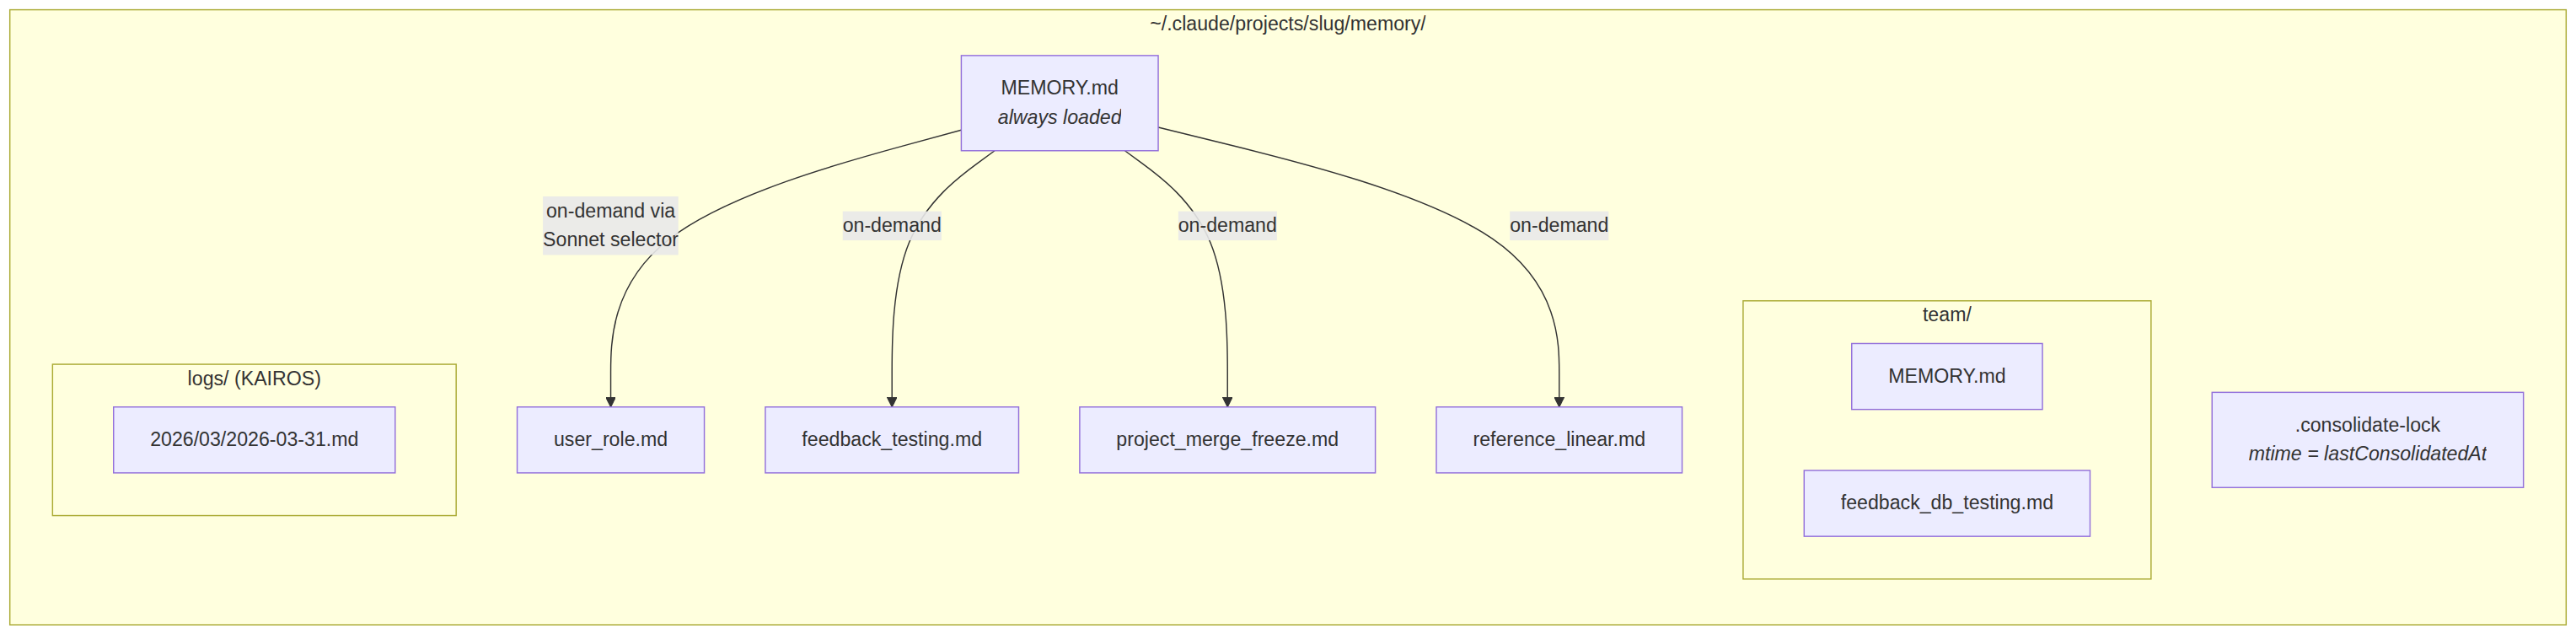
\includegraphics[width=21.99in,height=5.42in]{book/ch11-memory_files/figure-latex/mermaid-figure-1.png}

The naming convention is semantic:
\texttt{\textless{}type\textgreater{}\_\textless{}topic\textgreater{}.md}.
The type prefix is not enforced by code but is part of the prompt's
instructions, making it easy to visually scan the directory and
understand the memory landscape.

\begin{center}\rule{0.5\linewidth}{0.5pt}\end{center}

\section{The Four-Type Taxonomy}\label{the-four-type-taxonomy}

Not everything is worth remembering. The memory system constrains all
memories to exactly four types:

The four types are: \textbf{user}, \textbf{feedback}, \textbf{project},
and \textbf{reference}.

The taxonomy is designed around a single criterion: \textbf{is this
knowledge derivable from the current project state?} Code patterns,
architecture, file structure, git history -- all of these can be
re-derived by reading the codebase. They are excluded. The four types
capture what cannot be re-derived.

\textbf{User memories} record information about the person: their role,
goals, responsibilities, expertise level. A senior Go engineer who is
new to React gets different explanations than a first-time programmer.

\textbf{Feedback memories} capture guidance about how to approach work
-- both corrections and confirmations. The system explicitly instructs
the model to record both: ``if you only save corrections, you will drift
away from approaches the user has already validated.'' Each feedback
memory has a specific structure: the rule itself, then a
\texttt{**Why:**} line with the reason (often a past incident), then a
\texttt{**How\ to\ apply:**} line with the trigger conditions.

\textbf{Project memories} record ongoing work context -- who is doing
what, why, by when. The prompt emphasizes converting relative dates to
absolute: ``Thursday'' becomes ``2026-03-05'' so the memory remains
interpretable weeks later.

\textbf{Reference memories} are bookmarks -- pointers to where
information lives in external systems. A Linear project URL, a Grafana
dashboard, a Slack channel. These tell the model where to look, not what
to find.

\subsection{The Taxonomy as Filter}\label{the-taxonomy-as-filter}

The four types are not just categories -- they are a filter. By defining
exactly what counts as a memory, the system implicitly defines what does
not. Without the taxonomy, an eager model would save everything: code
patterns, architecture diagrams, error messages. All derivable from the
codebase. Saving it creates a parallel, potentially stale copy of
information that is better sourced from its origin.

The taxonomy also prevents a subtler failure: memory as crutch. If the
model saves architectural decisions as memories, it stops reading the
codebase to understand architecture. By excluding derivable information,
the system forces the model to stay grounded in the current state of the
code.

The exclusion list is explicit: code patterns, git history, debugging
solutions, anything in CLAUDE.md, ephemeral task details. These
exclusions apply even when the user explicitly asks to save. If a user
says ``remember this PR list,'' the model is instructed to push back --
``what was \emph{surprising} or \emph{non-obvious} about it?'' That
surprising part is worth keeping. The raw list is not. This instruction
was validated through evals, going from 0/2 to 3/3 when the
exclusion-override instruction was added.

\subsection{Frontmatter as Contract}\label{frontmatter-as-contract}

Every memory file uses YAML frontmatter with three required fields:

\begin{Shaded}
\begin{Highlighting}[]
\CommentTok{{-}{-}{-}}
\AnnotationTok{name:}\CommentTok{ \{\{memory name\}\}}
\AnnotationTok{description:}\CommentTok{ \{\{one{-}line description {-}{-} used to decide relevance\}\}}
\AnnotationTok{type:}\CommentTok{ \{\{user, feedback, project, reference\}\}}
\CommentTok{{-}{-}{-}}
\end{Highlighting}
\end{Shaded}

The \texttt{description} is the most load-bearing field. It is what the
relevance selector (a Sonnet side-query, discussed below) uses to decide
whether to surface this memory. A vague description like ``testing
stuff'' will either match too broadly or fail to match at all. A
specific description like ``Integration tests must hit real DB, not
mocks -- burned by mock divergence Q4'' matches exactly the
conversations where it matters. The description is the memory's search
index -- consumed not by a search engine but by a language model that
can understand nuance, context, and intent.

The frontmatter is also the only part of the file that the scanning
system reads during recall. \texttt{scanMemoryFiles()} reads each file
only to its first 30 lines to extract the header. The body is private
until the file is explicitly selected and loaded.

\begin{center}\rule{0.5\linewidth}{0.5pt}\end{center}

\section{The Write Path}\label{the-write-path}

Writing a memory is a two-step process executed with standard file
tools.

\textbf{Step 1: Write the memory file.} The model creates a \texttt{.md}
file in the memory directory with YAML frontmatter:

\begin{Shaded}
\begin{Highlighting}[]
\CommentTok{{-}{-}{-}}
\AnnotationTok{name:}\CommentTok{ Testing Policy}
\AnnotationTok{description:}\CommentTok{ Integration tests must hit real DB, not mocks}
\AnnotationTok{type:}\CommentTok{ feedback}
\CommentTok{{-}{-}{-}}

\NormalTok{Don\textquotesingle{}t mock the database in integration tests.}

\NormalTok{**Why:** We got burned last quarter when mocked tests passed but production}
\NormalTok{queries hit edge cases the mocks didn\textquotesingle{}t cover.}

\NormalTok{**How to apply:** Any test file under }\InformationTok{\textasciigrave{}\_\_tests\_\_/\textasciigrave{}}\NormalTok{ that touches database}
\NormalTok{operations should use the real PGlite instance from test{-}utils.}
\end{Highlighting}
\end{Shaded}

\textbf{Step 2: Update the index.} The model adds a one-line pointer to
\texttt{MEMORY.md}:

\begin{Shaded}
\begin{Highlighting}[]
\SpecialStringTok{{-} }\CommentTok{[}\OtherTok{Testing Policy}\CommentTok{](feedback\_testing.md)}\NormalTok{ {-}{-} integration tests must hit real DB}
\end{Highlighting}
\end{Shaded}

Each entry must stay under approximately 150 characters. The index is a
table of contents, not a knowledge base.

When the model learns new information that modifies an existing memory,
it uses \texttt{FileEditTool} to update the existing file rather than
creating a duplicate. The system does not version memories internally --
the file is on the local filesystem, and the user has \texttt{git} if
they want versioning. Before the prompt is built,
\texttt{ensureMemoryDirExists()} creates the memory directory, and the
prompt tells the model the directory already exists, avoiding wasted
turns on \texttt{ls} and \texttt{mkdir\ -p}.

\begin{center}\rule{0.5\linewidth}{0.5pt}\end{center}

\section{The Recall Path}\label{the-recall-path}

Writing memories is necessary but not sufficient. The harder problem is
retrieval: given a user's query, which of the potentially hundreds of
memory files should be loaded into the model's context? Loading all of
them would exhaust the token budget. Loading none would defeat the
purpose. Loading the wrong ones would waste tokens on irrelevant
information while missing the knowledge that would have changed the
model's behavior.

The recall system operates in two tiers. The \texttt{MEMORY.md} index is
always loaded into context at session start, providing orientation.
Individual memory files are surfaced on-demand through an LLM-powered
relevance query that selects up to five memories per turn.

\subsection{The Full Recall Pipeline}\label{the-full-recall-pipeline}

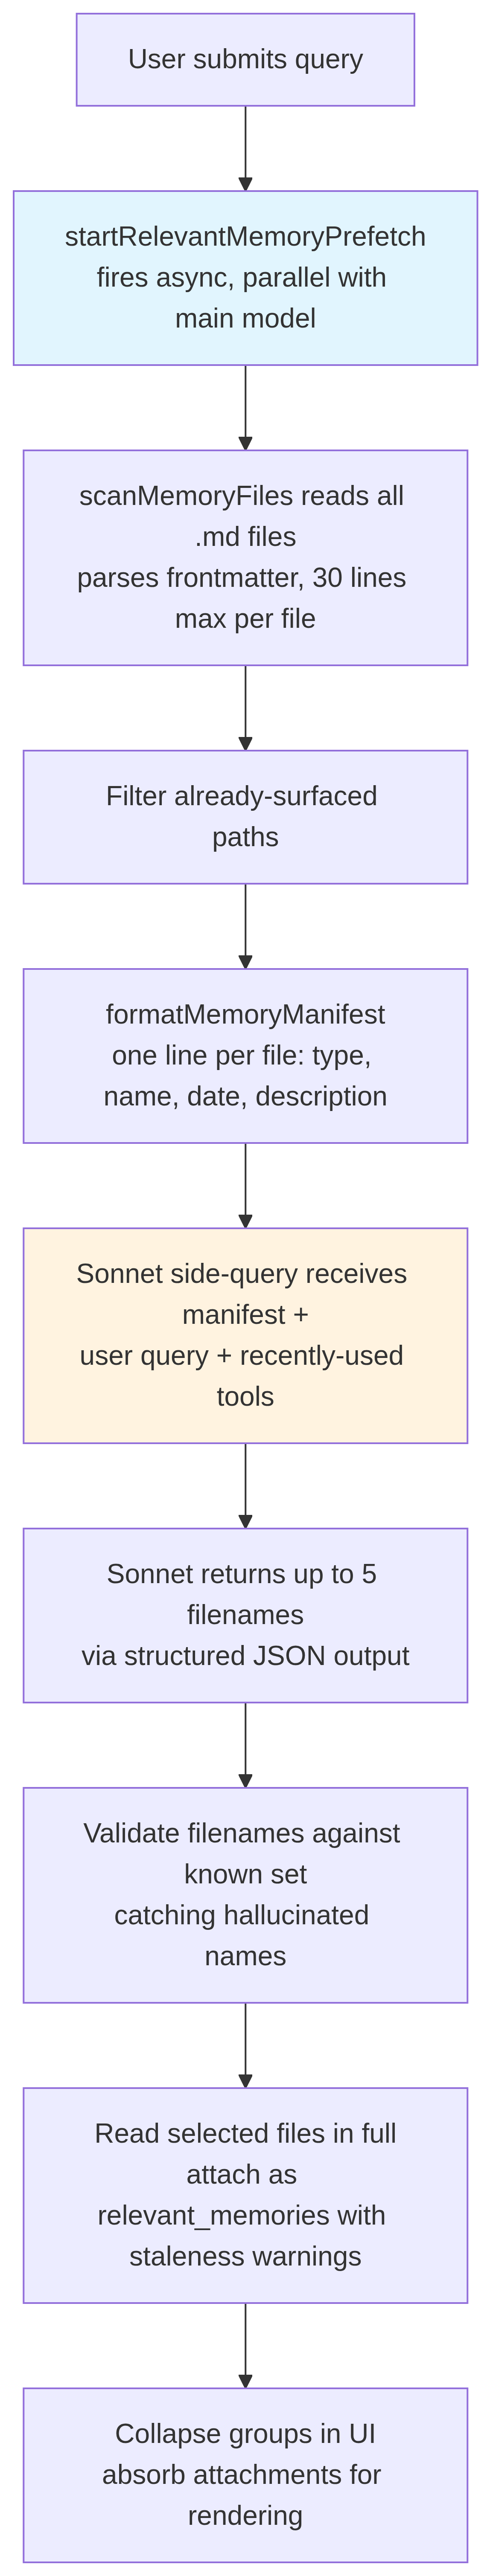
\includegraphics[width=3in,height=15.73in]{book/ch11-memory_files/figure-latex/mermaid-figure-3.png}

The async prefetch in step 2 is the key performance decision. By the
time the main model reaches a point where recalled context would be
useful, the side-query has usually already completed. The user
experiences no additional latency.

\subsection{The Sonnet Side-Query}\label{the-sonnet-side-query}

The manifest is sent to a Sonnet model as a side-query. The system
prompt for this selector is precise:

The system prompt for the selector instructs it to be conservative:
include only memories that will be useful for the current query, skip
memories if uncertain, and avoid selecting API/usage documentation for
tools already in active use (since the model already has those tools
loaded) -- but still surface warnings, gotchas, or known issues about
those tools.

The response uses structured output --
\texttt{\{\ selected\_memories:\ string{[}{]}\ \}} -- and filenames are
validated against the known set.

This approach trades latency for precision, and the tradeoff analysis is
instructive. \textbf{Keyword matching} would be fast but has no
understanding of context -- it cannot express ``do not select memories
for tools already in active use.'' \textbf{Embedding similarity} handles
semantic matching but introduces infrastructure (embedding model, vector
store, update pipeline) and struggles with negation -- the embedding of
``do NOT use database mocks'' is very close to ``use database mocks.''
\textbf{The Sonnet side-query} understands semantic relevance, reasons
about context, handles negation, and requires zero infrastructure. The
latency cost is bounded (hundreds of milliseconds) and hidden behind the
main model's initial processing.

The telemetry system tracks selection rates even when no memories are
selected. A selection rate of 0/150 means something different from 0/3
-- the first indicates a precision problem, the second a coverage
problem.

\begin{center}\rule{0.5\linewidth}{0.5pt}\end{center}

\section{Staleness}\label{staleness}

The staleness system addresses a failure mode that emerged from real
usage. Users reported that old memories -- containing file:line
citations to code that had since changed -- were being asserted as fact
by the model. The citation made the stale claim sound \emph{more}
authoritative, not less.

The solution is not expiration. Old memories are not deleted -- they may
contain institutional knowledge valid for years. Instead, the system
attaches age warnings:

The staleness function computes the memory's age in days. Memories from
today or yesterday get no warning (the function returns an empty
string). Everything older gets a caveat injected alongside the memory
content: a message stating the age in days and warning that code
behavior claims or file:line citations may be outdated, advising
verification against current code.

Memories from today or yesterday get no warning. Everything older gets a
staleness caveat injected alongside the memory content. The
human-readable format -- ``today,'' ``yesterday,'' ``47 days ago'' --
exists because models are poor at date arithmetic. A raw ISO timestamp
does not trigger staleness reasoning the way ``47 days ago'' does. This
is an empirical observation about model behavior, validated through
evals: the action-cue framing ``Before recommending from memory'' scored
3/3 versus 0/3 for the more abstract ``Trusting what you recall,'' with
identical body text.

There is a philosophical tension worth naming. The staleness system
treats memories as hypotheses, not facts. But the model's natural
tendency is to present information confidently. The staleness warning is
fighting the model's own voice -- using its instruction-following
capability to override its confidence-generation tendency.

\begin{center}\rule{0.5\linewidth}{0.5pt}\end{center}

\section{MEMORY.md as the Always-Loaded
Index}\label{memory.md-as-the-always-loaded-index}

Every conversation begins with \texttt{MEMORY.md} in context. It is not
a memory -- it is an index, a table of contents for the actual memory
files.

The index has two hard caps:

The index has two hard caps: 200 lines and 25,000 bytes.

The 200-line cap catches normal growth. The 25KB byte cap catches an
observed failure mode: users packing long lines that stay under 200
lines but consume enormous token budgets. At the 97th percentile, a
MEMORY.md with only 197 lines weighed 197KB. When either cap fires,
actionable guidance tells the user what to fix: ``Keep index entries to
one line under \textasciitilde200 chars; move detail into topic files.''

This two-tier architecture -- lightweight always-on index plus heavy
on-demand content -- is the design that allows memory to scale. A
project with 150 memories has a 150-line index consuming perhaps 3,000
tokens, not 150 full files consuming 100,000.

\begin{center}\rule{0.5\linewidth}{0.5pt}\end{center}

The transition from individual memory to shared knowledge is natural. A
testing policy, a deployment convention, a known gotcha in the build
system -- these need to be shared across a team.

\section{Team Memory}\label{team-memory}

Team memory is a subdirectory of the auto-memory directory at
\texttt{\textless{}autoMemPath\textgreater{}/team/}, gated behind a
feature flag and requiring auto-memory to be enabled. The architectural
nesting is deliberate: disabling auto-memory transitively disables team
memory.

\subsection{Defense in Depth}\label{defense-in-depth}

Team memory introduces an attack surface that individual memory does not
have. Team-synced files come from other users, and a malicious teammate
could attempt path traversal. The security model uses three layers of
defense.

\textbf{Layer 1: Input sanitization.} The \texttt{sanitizePathKey()}
function validates against null bytes, URL-encoded traversals
(\texttt{\%2e\%2e\%2f}), Unicode normalization attacks (fullwidth
characters that normalize to \texttt{../}), backslashes, and absolute
paths.

\textbf{Layer 2: String-level path validation.} After sanitization,
\texttt{path.resolve()} normalizes remaining \texttt{..} segments, and
the resolved path is checked against the team directory prefix
(including a trailing separator to prevent \texttt{team-evil/} from
matching \texttt{team/}).

\textbf{Layer 3: Symlink resolution.} \texttt{realpathDeepestExisting()}
resolves symlinks on the deepest existing ancestor, catching attacks
that string-level validation cannot detect. If \texttt{team/evil} is a
symlink pointing to \texttt{/etc/}, string validation sees a valid
prefix, but \texttt{realpath} reveals the true target.

All validation failures produce a \texttt{PathTraversalError}. No
partial successes, no fallbacks. Fail closed.

\subsection{Scope Guidance}\label{scope-guidance}

The prompt teaches the model about private vs.~shared memory. User
memories are always private. Reference memories are usually team.
Feedback memories default to private unless they represent project-wide
conventions. The cross-checking instruction -- ``Before saving a private
feedback memory, check that it does not contradict a team feedback
memory'' -- prevents conflicting guidance from surfacing unpredictably
depending on which memory is recalled first.

\begin{center}\rule{0.5\linewidth}{0.5pt}\end{center}

\section{KAIROS Mode: Append-Only Daily
Logs}\label{kairos-mode-append-only-daily-logs}

Standard memory assumes discrete sessions. KAIROS mode (Claude Code's
assistant mode) breaks this assumption -- sessions are long-lived,
potentially running for days. The two-step write pattern does not scale
to continuous operation.

The solution is architectural separation between capture and
consolidation:

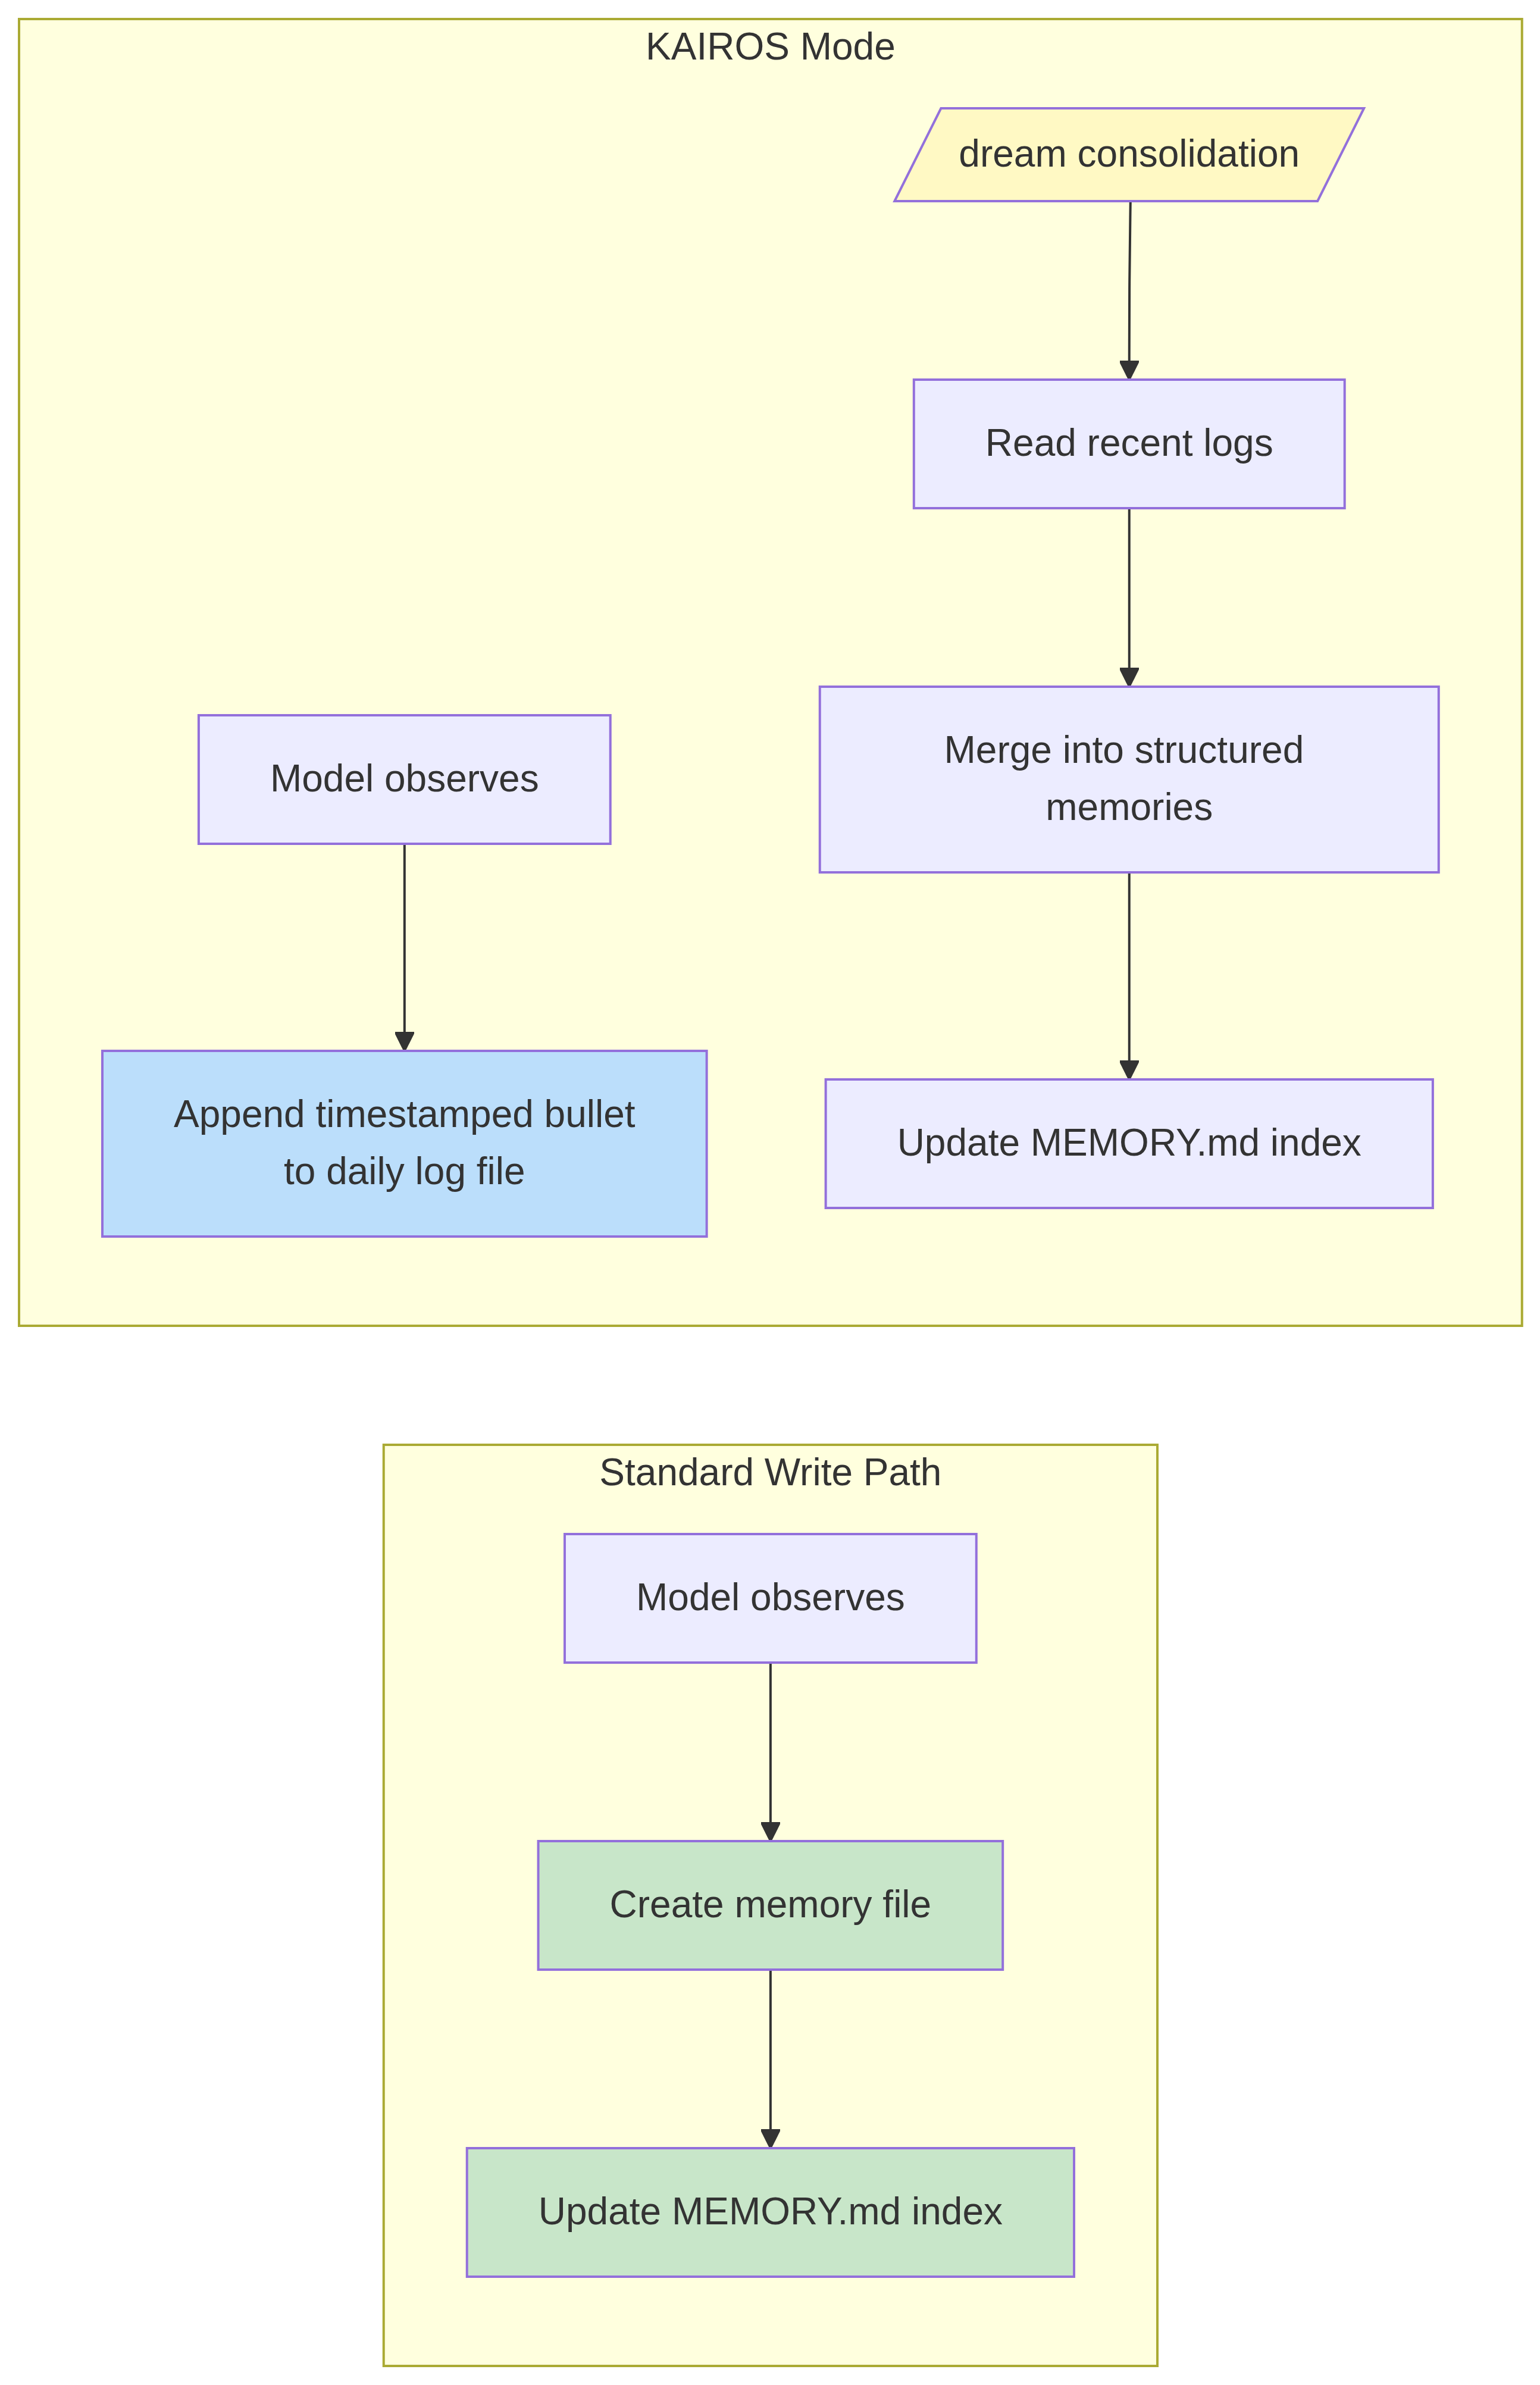
\includegraphics[width=6.74in,height=10.44in]{book/ch11-memory_files/figure-latex/mermaid-figure-2.png}

In KAIROS mode, the model appends to date-named log files
(\texttt{\textless{}autoMemPath\textgreater{}/logs/YYYY/MM/YYYY-MM-DD.md}).
Each entry is a short timestamped bullet. The model is instructed: ``Do
not rewrite or reorganize the log'' -- restructuring during capture
loses the chronological signal that consolidation needs.

The path in the prompt is described as a \emph{pattern} rather than
today's literal date. This is a caching optimization: the memory prompt
is cached and not invalidated when the date changes at midnight. The
model derives the current date from a separate \texttt{date\_change}
attachment.

\subsection{The /dream Consolidation}\label{the-dream-consolidation}

Consolidation runs in four phases: \textbf{Orient} (list directory, read
index, skim existing files), \textbf{Gather} (search logs, check for
drifted memories), \textbf{Consolidate} (write or update files, merge
rather than duplicate), \textbf{Prune} (update index under 200 lines,
remove stale pointers). The emphasis on merging into existing files
rather than creating new ones is important -- without it, the memory
directory would grow linearly with usage.

\subsection{The Consolidation Lock}\label{the-consolidation-lock}

The lock file \texttt{.consolidate-lock} serves dual purpose: its
content is the holder's PID (mutual exclusion), its mtime \emph{is}
\texttt{lastConsolidatedAt} (scheduling state). The auto-dream fires
when three gates pass, evaluated cheapest-first: hours since last
consolidation exceeds 24, sessions modified since then exceeds 5, and no
other process holds the lock. Crash recovery detects dead PIDs via
\texttt{process.kill(pid,\ 0)}, with a one-hour staleness timeout as
defense against PID reuse.

\begin{center}\rule{0.5\linewidth}{0.5pt}\end{center}

\section{Background Extraction}\label{background-extraction}

The main agent has full instructions for writing memories proactively.
But agents are imperfect -- and the imperfection is predictable. When a
user says ``remember to always use integration tests'' and then
immediately asks ``now fix the login bug,'' the model's attention shifts
entirely to the bug. The memory-saving instruction was processed but may
not execute.

At the end of each complete query loop, a forked agent -- sharing the
parent's prompt cache -- analyzes recent messages and writes any
memories the main agent missed. When the main agent has already written
memories in the current turn range, the extraction agent skips that
range. The extraction agent has a constrained tool budget: read-only
tools plus write access only to memory directory paths. Its prompt
instructs a two-turn strategy: turn 1 reads in parallel, turn 2 writes
in parallel.

The interaction is cooperative, not competitive. The main agent's prompt
always contains the full save instructions. When the main agent saves,
the background agent defers. When it does not, the background agent
catches the gap. This pattern -- a primary path with a background safety
net -- makes memory capture more reliable without burdening the primary
interaction. Neither alone would be sufficient.

\begin{center}\rule{0.5\linewidth}{0.5pt}\end{center}

\section{Path Resolution and
Security}\label{path-resolution-and-security}

The auto-memory path is resolved through a priority chain:

\begin{enumerate}
\def\labelenumi{\arabic{enumi}.}
\tightlist
\item
  \textbf{\texttt{CLAUDE\_COWORK\_MEMORY\_PATH\_OVERRIDE}} -- Full-path
  override for Cowork.
\item
  \textbf{\texttt{autoMemoryDirectory} in settings.json} -- Only trusted
  settings sources. Project settings are intentionally excluded.
\item
  \textbf{Default computed path} --
  \texttt{\textasciitilde{}/.claude/projects/\textless{}sanitized-git-root\textgreater{}/memory/}.
\end{enumerate}

The exclusion of project settings is a security decision. A malicious
repository could commit \texttt{.claude/settings.json} with
\texttt{autoMemoryDirectory:\ "\textasciitilde{}/.ssh"}, and the
permission carve-out for memory files would grant the model automatic
write access to SSH keys. By limiting the override to policy, flag,
local, and user settings -- none committable to a repository -- this
attack vector is closed.

The \texttt{isAutoMemPath()} function normalizes paths before
prefix-checking to prevent traversal, and the trailing separator
convention ensures prefix matching requires a directory boundary.

\subsection{The Enable/Disable Chain}\label{the-enabledisable-chain}

Whether auto-memory is active is determined by
\texttt{isAutoMemoryEnabled()}, implementing its own priority chain:
environment variable, bare mode, CCR without persistent storage,
settings, default enabled. When disabled, both the prompt section is
dropped (so the model receives no memory instructions) and the
background processes stop (extract-memories, auto-dream, team sync).
Both gates must align -- removing the prompt alone would not stop the
extraction agent, which has its own prompt.

\begin{center}\rule{0.5\linewidth}{0.5pt}\end{center}

\section{Apply This: Designing Agent
Memory}\label{apply-this-designing-agent-memory}

The memory system's complexity is in the behavioral layer -- prompt
instructions, LLM-powered recall, staleness management, background
extraction -- not in storage infrastructure. This distribution of
complexity is itself a design principle.

\textbf{Files beat databases for agent memory.} Files are inspectable,
editable, and version-controllable. Transparency builds trust. When the
alternative is a database users cannot easily read, files win on trust
alone.

\textbf{Constrain what gets saved, not just how.} The derivability test
-- can this knowledge be re-derived from the current project state? --
eliminates the majority of potential memories while preserving the ones
that actually matter.

\textbf{Use an LLM for recall, not keywords or embeddings.} An LLM
side-query understands context, reasons about what is already available
in conversation, handles negation, and requires no index maintenance.
The latency cost is real but bounded and hidden behind the main model's
processing.

\textbf{Warn about staleness, do not expire.} Institutional knowledge
may remain valid for years. Attaching age warnings lets the model treat
old memories as hypotheses rather than facts. The human-readable age
format triggers the right reasoning in a way that raw timestamps do not.

\textbf{Build a safety net for capture.} The main agent will miss
memories. A background extraction agent that reviews recent conversation
makes the system more reliable without burdening the primary
interaction. When the main agent saves, the background agent defers.

\begin{center}\rule{0.5\linewidth}{0.5pt}\end{center}

The agent can now learn across sessions -- accumulating knowledge about
its user, their preferences, their project's state, and the corrections
they have made. The memory system makes a philosophical commitment: that
an agent's relationship with its user should deepen over time, not reset
on every interaction. The file-based implementation makes that
commitment tangible -- visible on disk, editable by humans,
version-controlled alongside code. The agent's memory is not a black
box. It is a collection of notes in a folder, written in a language that
both the model and the human can read.

The next chapter examines how Claude Code extends its capabilities
beyond the core: the skills system that teaches the model new behaviors,
and the hooks system that lets external code constrain and modify those
behaviors at over two dozen lifecycle points.

\chapter{Chapter 12: Extensibility -- Skills and
Hooks}\label{chapter-12-extensibility-skills-and-hooks}

\section{Two Dimensions of Extension}\label{two-dimensions-of-extension}

Every extensibility system answers two questions: what can the system
do, and when does it do it. Most frameworks conflate the two -- a plugin
registers both capabilities and lifecycle callbacks in the same object,
and the boundary between ``adding a feature'' and ``intercepting a
feature'' blurs into a single registration API.

Claude Code separates them cleanly. Skills extend what the model can do.
They are markdown files that become slash commands, injecting new
instructions into the conversation when invoked. Hooks extend when and
how things happen. They are lifecycle interceptors that fire at over two
dozen distinct points during a session, running arbitrary code that can
block actions, modify inputs, force continuation, or silently observe.

The separation is not accidental. Skills are content -- they expand the
model's knowledge and capabilities by adding prompt text. Hooks are
control flow -- they modify the execution path without changing what the
model knows. A skill might teach the model how to run your team's
deployment process. A hook might ensure no deployment command executes
without a passing test suite. The skill adds capability; the hook adds
constraint.

This chapter covers both systems in depth, then examines where they
intersect: skill-declared hooks that register as session-scoped
lifecycle interceptors when the skill is invoked.

\begin{center}\rule{0.5\linewidth}{0.5pt}\end{center}

\section{Skills: Teaching the Model New
Tricks}\label{skills-teaching-the-model-new-tricks}

\subsection{Two-Phase Loading}\label{two-phase-loading}

The core optimization of the skills system is that frontmatter loads at
startup, but full content loads only on invocation.

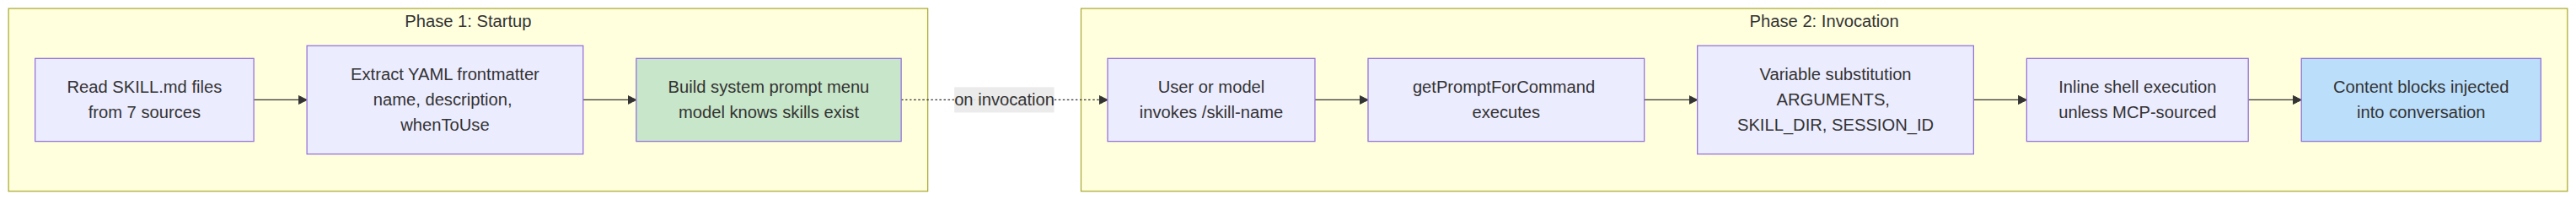
\includegraphics[width=25.26in,height=1.96in]{book/ch12-extensibility_files/figure-latex/mermaid-figure-1.png}

\textbf{Phase 1} reads each \texttt{SKILL.md} file, splits YAML
frontmatter from the markdown body, and extracts metadata. The
frontmatter fields become part of the system prompt so the model knows
the skill exists. The markdown body is captured in a closure but not
processed. A project with 50 skills pays the token cost of 50 short
descriptions, not 50 full documents.

\textbf{Phase 2} fires when the model or user invokes a skill.
\texttt{getPromptForCommand} prepends the base directory, substitutes
variables (\texttt{\$ARGUMENTS}, \texttt{\$\{CLAUDE\_SKILL\_DIR\}},
\texttt{\$\{CLAUDE\_SESSION\_ID\}}), and executes inline shell commands
(backtick-prefixed with \texttt{!}). The result is returned as content
blocks injected into the conversation.

\subsection{Seven Sources with
Priority}\label{seven-sources-with-priority}

Skills arrive from seven distinct sources, loaded in parallel and merged
by precedence:

\begin{longtable}[]{@{}
  >{\raggedright\arraybackslash}p{(\linewidth - 6\tabcolsep) * \real{0.2857}}
  >{\raggedright\arraybackslash}p{(\linewidth - 6\tabcolsep) * \real{0.2286}}
  >{\raggedright\arraybackslash}p{(\linewidth - 6\tabcolsep) * \real{0.2857}}
  >{\raggedright\arraybackslash}p{(\linewidth - 6\tabcolsep) * \real{0.2000}}@{}}
\toprule\noalign{}
\begin{minipage}[b]{\linewidth}\raggedright
Priority
\end{minipage} & \begin{minipage}[b]{\linewidth}\raggedright
Source
\end{minipage} & \begin{minipage}[b]{\linewidth}\raggedright
Location
\end{minipage} & \begin{minipage}[b]{\linewidth}\raggedright
Notes
\end{minipage} \\
\midrule\noalign{}
\endhead
\bottomrule\noalign{}
\endlastfoot
1 & Managed (Policy) &
\texttt{\textless{}MANAGED\_PATH\textgreater{}/.claude/skills/} &
Enterprise-controlled \\
2 & User & \texttt{\textasciitilde{}/.claude/skills/} & Personal,
available everywhere \\
3 & Project & \texttt{.claude/skills/} (walked up to home) & Checked
into version control \\
4 & Additional Dirs &
\texttt{\textless{}add-dir\textgreater{}/.claude/skills/} & Via
\texttt{-\/-add-dir} flag \\
5 & Legacy Commands & \texttt{.claude/commands/} &
Backwards-compatible \\
6 & Bundled & Compiled into the binary & Feature-gated \\
7 & MCP & MCP server prompts & Remote, untrusted \\
\end{longtable}

Deduplication uses \texttt{realpath} to resolve symlinks and overlapping
parent directories. The first-seen source wins. The
\texttt{getFileIdentity} function resolves to canonical paths via
\texttt{realpath} rather than relying on inode values, which are
unreliable on container/NFS mounts and ExFAT.

\subsection{The Frontmatter Contract}\label{the-frontmatter-contract}

Key frontmatter fields that control skill behavior:

\begin{longtable}[]{@{}ll@{}}
\toprule\noalign{}
YAML Field & Purpose \\
\midrule\noalign{}
\endhead
\bottomrule\noalign{}
\endlastfoot
\texttt{name} & User-facing display name \\
\texttt{description} & Shown in autocomplete and system prompt \\
\texttt{when\_to\_use} & Detailed usage scenarios for model discovery \\
\texttt{allowed-tools} & Which tools the skill can use \\
\texttt{disable-model-invocation} & Block autonomous model use \\
\texttt{context} & \texttt{\textquotesingle{}fork\textquotesingle{}} to
run as sub-agent \\
\texttt{hooks} & Lifecycle hooks registered on invocation \\
\texttt{paths} & Glob patterns for conditional activation \\
\end{longtable}

The \texttt{context:\ \textquotesingle{}fork\textquotesingle{}} option
runs the skill as a sub-agent with its own context window, essential for
skills that need significant work without polluting the main
conversation's token budget. The \texttt{disable-model-invocation} and
\texttt{user-invocable} fields control two distinct access paths --
setting both to true makes the skill invisible, useful for hooks-only
skills.

\subsection{The MCP Security Boundary}\label{the-mcp-security-boundary}

After variable substitution, inline shell commands execute. The security
boundary is absolute: \textbf{MCP skills never execute inline shell
commands.} MCP servers are external systems. An MCP prompt containing
\texttt{!\textasciigrave{}rm\ -rf\ /\textasciigrave{}} would execute
with the user's full permissions if allowed. The system treats MCP
skills as content-only. This trust boundary connects to the broader MCP
security model discussed in Chapter 15.

\subsection{Dynamic Discovery}\label{dynamic-discovery}

Skills are not only loaded at startup. When the model touches files,
\texttt{discoverSkillDirsForPaths} walks up from each path looking for
\texttt{.claude/skills/} directories. Skills with \texttt{paths}
frontmatter are stored in a \texttt{conditionalSkills} map and activate
only when touched paths match their patterns. A skill declaring
\texttt{paths:\ "packages/database/**"} remains invisible until the
model reads or edits a database file -- context-sensitive capability
expansion.

\begin{center}\rule{0.5\linewidth}{0.5pt}\end{center}

\section{Hooks: Controlling When Things
Happen}\label{hooks-controlling-when-things-happen}

Hooks are Claude Code's mechanism for intercepting and modifying
behavior at lifecycle points. The main execution engine exceeds 4,900
lines. The system serves three audiences: individual developers (custom
linting, validation), teams (shared quality gates checked into the
project), and enterprises (policy-managed compliance rules).

\subsection{A Real-World Hook: Preventing Commits to
Main}\label{a-real-world-hook-preventing-commits-to-main}

Before diving into the machinery, here is what a hook looks like in
practice. Suppose your team wants to prevent the model from committing
directly to the \texttt{main} branch.

\textbf{Step 1: The settings.json configuration:}

\begin{Shaded}
\begin{Highlighting}[]
\FunctionTok{\{}
  \DataTypeTok{"hooks"}\FunctionTok{:} \FunctionTok{\{}
    \DataTypeTok{"PreToolUse"}\FunctionTok{:} \OtherTok{[}
      \FunctionTok{\{}
        \DataTypeTok{"matcher"}\FunctionTok{:} \StringTok{"Bash"}\FunctionTok{,}
        \DataTypeTok{"hooks"}\FunctionTok{:} \OtherTok{[}
          \FunctionTok{\{}
            \DataTypeTok{"type"}\FunctionTok{:} \StringTok{"command"}\FunctionTok{,}
            \DataTypeTok{"command"}\FunctionTok{:} \StringTok{"/path/to/check{-}not{-}main.sh"}\FunctionTok{,}
            \DataTypeTok{"if"}\FunctionTok{:} \StringTok{"Bash(git commit*)"}
          \FunctionTok{\}}
        \OtherTok{]}
      \FunctionTok{\}}
    \OtherTok{]}
  \FunctionTok{\}}
\FunctionTok{\}}
\end{Highlighting}
\end{Shaded}

\textbf{Step 2: The shell script:}

\begin{Shaded}
\begin{Highlighting}[]
\CommentTok{\#!/bin/bash}
\VariableTok{BRANCH}\OperatorTok{=}\VariableTok{$(}\FunctionTok{git}\NormalTok{ rev{-}parse }\AttributeTok{{-}{-}abbrev{-}ref}\NormalTok{ HEAD }\DecValTok{2}\OperatorTok{\textgreater{}}\NormalTok{/dev/null}\VariableTok{)}
\ControlFlowTok{if} \BuiltInTok{[} \StringTok{"}\VariableTok{$BRANCH}\StringTok{"} \OtherTok{=} \StringTok{"main"} \BuiltInTok{]}\KeywordTok{;} \ControlFlowTok{then}
  \BuiltInTok{echo} \StringTok{"Cannot commit directly to main. Create a feature branch first."} \OperatorTok{\textgreater{}\&}\DecValTok{2}
  \BuiltInTok{exit}\NormalTok{ 2  }\CommentTok{\# Exit 2 = blocking error}
\ControlFlowTok{fi}
\BuiltInTok{exit}\NormalTok{ 0}
\end{Highlighting}
\end{Shaded}

\textbf{Step 3: What the model experiences.} When the model tries
\texttt{git\ commit} on the \texttt{main} branch, the hook fires before
the command executes. The script checks the branch, writes to stderr,
and exits with code 2. The model sees a system message: ``Cannot commit
directly to main. Create a feature branch first.'' The commit never
runs. The model creates a branch and commits there instead.

The \texttt{if:\ "Bash(git\ commit*)"} condition means the script only
runs for git commit commands -- not for every Bash invocation. Exit code
2 blocks; exit code 0 passes; any other exit code produces a
non-blocking warning. This is the complete protocol.

\subsection{Four User-Configurable
Types}\label{four-user-configurable-types}

Claude Code defines six hook types -- four user-configurable, two
internal.

\textbf{Command hooks} spawn a shell process. Hook input JSON is piped
to stdin; the hook communicates back via exit code and stdout/stderr.
This is the workhorse type.

\textbf{Prompt hooks} make a single LLM call, returning
\texttt{\{"ok":\ true\}} or
\texttt{\{"ok":\ false,\ "reason":\ "..."\}}. Lightweight AI-powered
validation without a full agent loop.

\textbf{Agent hooks} run a multi-turn agentic loop (max 50 turns,
\texttt{dontAsk} permissions, thinking disabled). Each gets its own
session scope. This is the heavy machinery for ``verify that the test
suite passes and covers the new feature.''

\textbf{HTTP hooks} POST the hook input to a URL. Enables remote policy
servers and audit logging without local process spawning.

The two internal types are \textbf{callback hooks} (registered
programmatically, -70\% overhead on the hot path via a fast path that
skips span tracking) and \textbf{function hooks} (session-scoped
TypeScript callbacks for structured output enforcement in agent hooks).

\subsection{The Five Most Important Lifecycle
Events}\label{the-five-most-important-lifecycle-events}

The hook system fires at over two dozen lifecycle points. Five dominate
real-world usage:

\textbf{PreToolUse} -- fires before every tool execution. Can block,
modify input, auto-approve, or inject context. Permission behavior
follows strict precedence: deny \textgreater{} ask \textgreater{} allow.
The most common hook point for quality gates.

\textbf{PostToolUse} -- fires after successful execution. Can inject
context or replace MCP tool output entirely. Useful for automated
feedback on tool results.

\textbf{Stop} -- fires before Claude concludes its response. A blocking
hook forces continuation. This is the mechanism for automated
verification loops: ``are you really done?''

\textbf{SessionStart} -- fires at session beginning. Can set environment
variables, override the first user message, or register file watch
paths. Cannot block (a hook cannot prevent a session from starting).

\textbf{UserPromptSubmit} -- fires when the user submits a prompt. Can
block processing, enabling input validation or content filtering before
the model sees it.

\textbf{Reference table -- remaining events:}

\begin{longtable}[]{@{}
  >{\raggedright\arraybackslash}p{(\linewidth - 2\tabcolsep) * \real{0.5556}}
  >{\raggedright\arraybackslash}p{(\linewidth - 2\tabcolsep) * \real{0.4444}}@{}}
\toprule\noalign{}
\begin{minipage}[b]{\linewidth}\raggedright
Category
\end{minipage} & \begin{minipage}[b]{\linewidth}\raggedright
Events
\end{minipage} \\
\midrule\noalign{}
\endhead
\bottomrule\noalign{}
\endlastfoot
Tool lifecycle & PostToolUseFailure, PermissionDenied,
PermissionRequest \\
Session & SessionEnd (1.5s timeout), Setup \\
Subagent & SubagentStart, SubagentStop \\
Compaction & PreCompact, PostCompact \\
Notification & Notification, Elicitation, ElicitationResult \\
Configuration & ConfigChange, InstructionsLoaded, CwdChanged,
FileChanged, TaskCreated, TaskCompleted, TeammateIdle \\
\end{longtable}

The blocking asymmetry is intentional. Events representing recoverable
decisions (tool calls, stop conditions) support blocking. Events
representing irrevocable facts (session started, API failed) do not.

\subsection{Exit Code Semantics}\label{exit-code-semantics}

For command hooks, exit codes carry specific meaning:

\begin{longtable}[]{@{}lll@{}}
\toprule\noalign{}
Exit Code & Meaning & Blocks \\
\midrule\noalign{}
\endhead
\bottomrule\noalign{}
\endlastfoot
0 & Success, stdout parsed if JSON & No \\
2 & Blocking error, stderr shown as system message & Yes \\
Other & Non-blocking warning, shown to user only & No \\
\end{longtable}

Exit code 2 was chosen deliberately. Exit code 1 is too common -- any
unhandled exception, assertion failure, or syntax error produces exit 1.
Using exit 2 prevents accidental enforcement.

\subsection{Six Hook Sources}\label{six-hook-sources}

\begin{longtable}[]{@{}
  >{\raggedright\arraybackslash}p{(\linewidth - 4\tabcolsep) * \real{0.2857}}
  >{\raggedright\arraybackslash}p{(\linewidth - 4\tabcolsep) * \real{0.4643}}
  >{\raggedright\arraybackslash}p{(\linewidth - 4\tabcolsep) * \real{0.2500}}@{}}
\toprule\noalign{}
\begin{minipage}[b]{\linewidth}\raggedright
Source
\end{minipage} & \begin{minipage}[b]{\linewidth}\raggedright
Trust Level
\end{minipage} & \begin{minipage}[b]{\linewidth}\raggedright
Notes
\end{minipage} \\
\midrule\noalign{}
\endhead
\bottomrule\noalign{}
\endlastfoot
\texttt{userSettings} & User &
\texttt{\textasciitilde{}/.claude/settings.json}, highest priority \\
\texttt{projectSettings} & Project & \texttt{.claude/settings.json},
version-controlled \\
\texttt{localSettings} & Local & \texttt{.claude/settings.local.json},
gitignored \\
\texttt{policySettings} & Enterprise & Cannot be overridden \\
\texttt{pluginHook} & Plugin & Priority 999 (lowest) \\
\texttt{sessionHook} & Session & In-memory only, registered by skills \\
\end{longtable}

\begin{center}\rule{0.5\linewidth}{0.5pt}\end{center}

\section{The Snapshot Security Model}\label{the-snapshot-security-model}

Hooks execute arbitrary code. A project's \texttt{.claude/settings.json}
can define hooks that fire before every tool call. What happens if a
malicious repository modifies its hooks after the user accepts the
workspace trust dialog?

Nothing. The hooks configuration is frozen at startup.

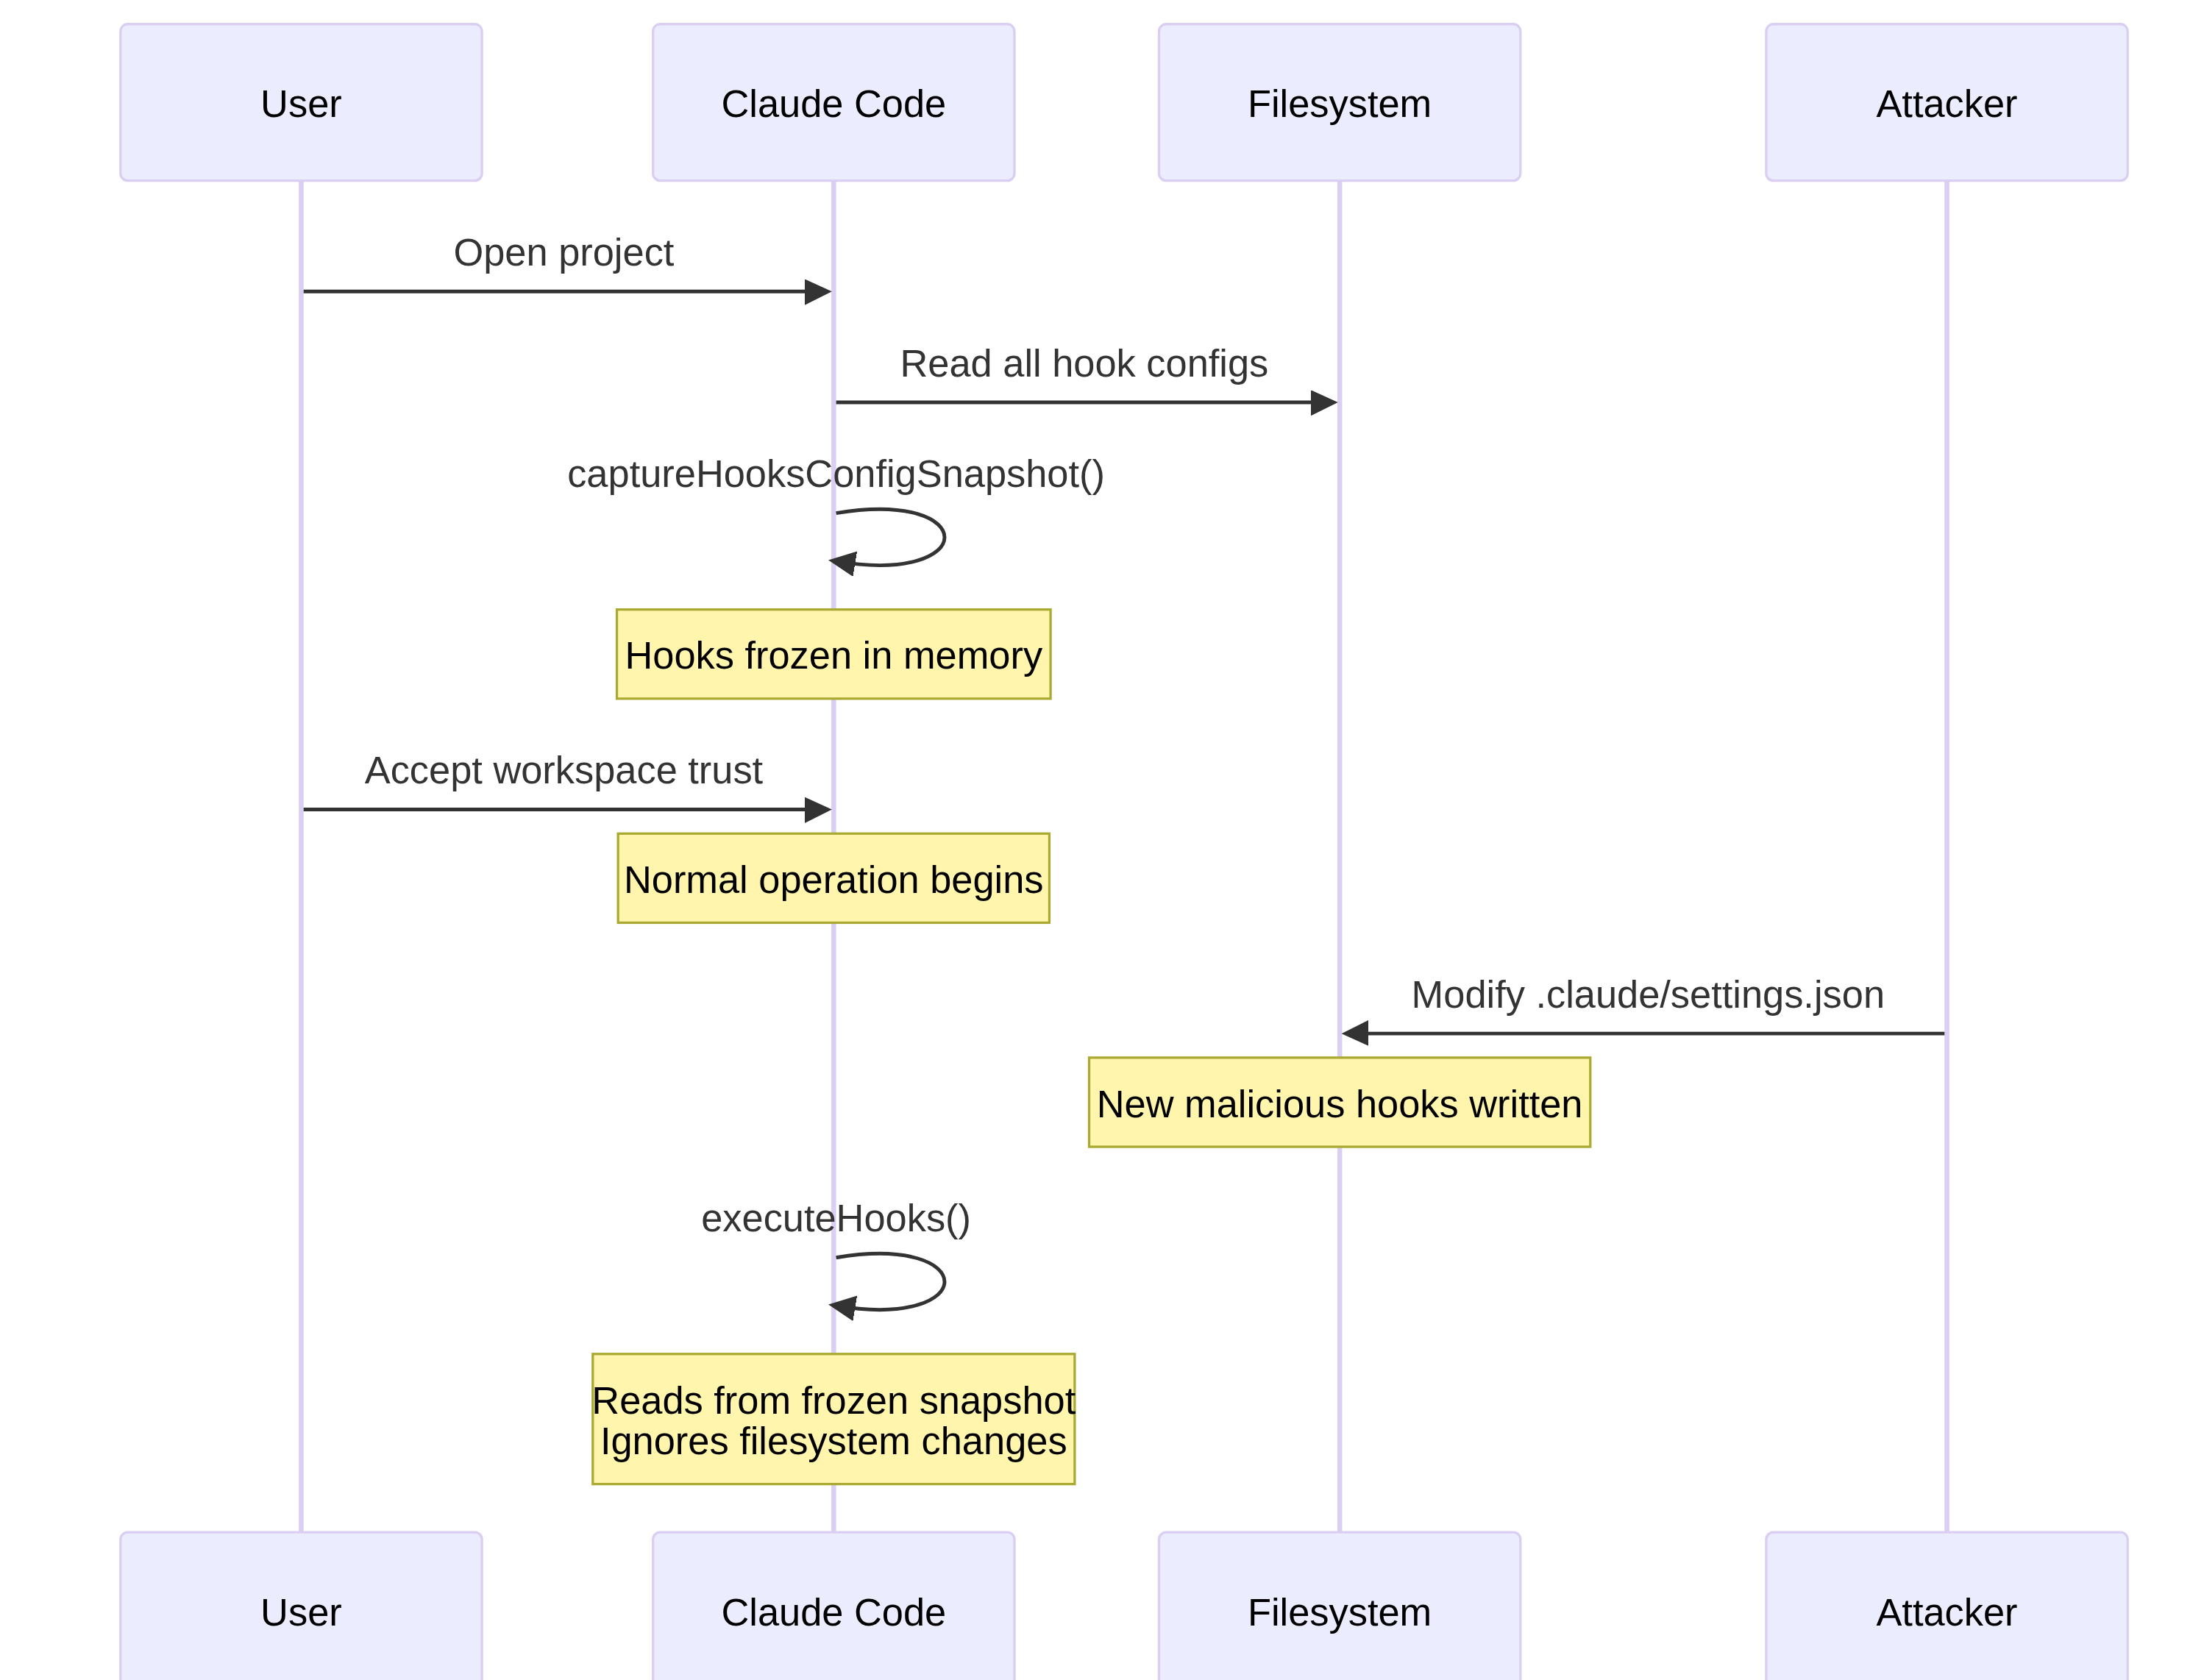
\includegraphics[width=9.72in,height=7.42in]{book/ch12-extensibility_files/figure-latex/mermaid-figure-3.png}

\texttt{captureHooksConfigSnapshot()} is called once during startup.
From that point, \texttt{executeHooks()} reads from the snapshot, never
re-reading settings files implicitly. The snapshot is only updated
through explicit channels: the \texttt{/hooks} command or a file watcher
detection, both of which rebuild through
\texttt{updateHooksConfigSnapshot()}.

The policy enforcement cascade: \texttt{disableAllHooks} in policy
settings clears everything. \texttt{allowManagedHooksOnly} excludes user
and project hooks. A user can disable their own hooks by setting
\texttt{disableAllHooks}, but they cannot disable enterprise-managed
hooks. The policy layer always wins.

The trust check itself (\texttt{shouldSkipHookDueToTrust()}) was
introduced after two vulnerabilities: SessionEnd hooks executing when a
user \emph{declined} the trust dialog, and SubagentStop hooks firing
before trust was presented. Both shared the same root cause -- hooks
firing in lifecycle states where the user had not consented to workspace
code execution. The fix is a centralized gate at the top of
\texttt{executeHooks()}.

\begin{center}\rule{0.5\linewidth}{0.5pt}\end{center}

\section{Execution Flow}\label{execution-flow}

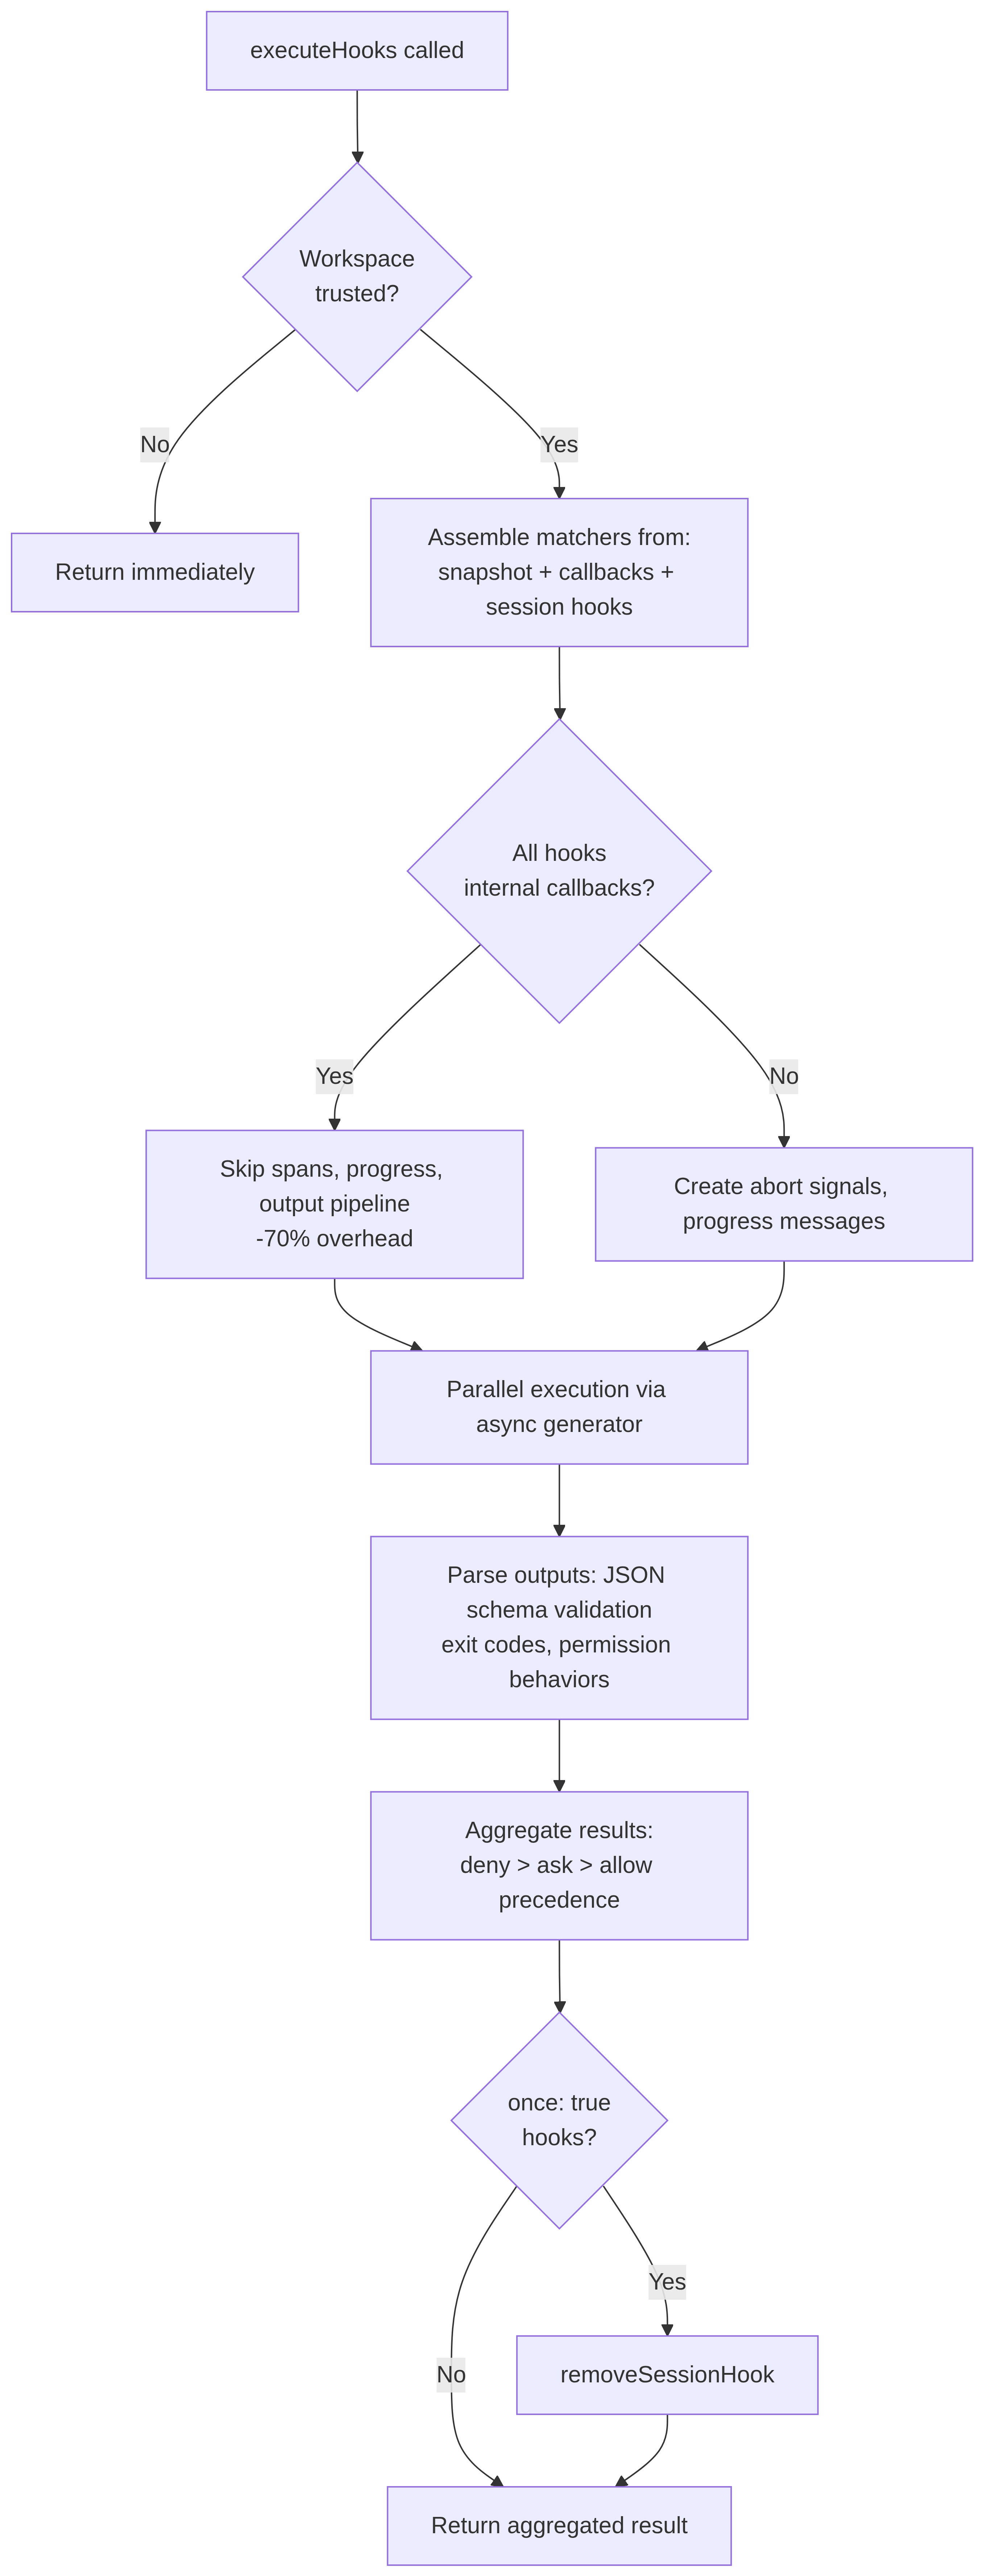
\includegraphics[width=7.07in,height=18.51in]{book/ch12-extensibility_files/figure-latex/mermaid-figure-2.png}

The fast path for internal callbacks is a significant optimization. When
all matched hooks are internal (file access analytics, commit
attribution), the system skips span tracking, abort signal creation,
progress messages, and the full output processing pipeline. Most
PostToolUse invocations hit only internal callbacks.

Hook input JSON is serialized once via a lazy \texttt{getJsonInput()}
closure and reused across all parallel hooks. Environment injection sets
\texttt{CLAUDE\_PROJECT\_DIR}, \texttt{CLAUDE\_PLUGIN\_ROOT}, and for
certain events, \texttt{CLAUDE\_ENV\_FILE} where hooks can write
environment exports.

\begin{center}\rule{0.5\linewidth}{0.5pt}\end{center}

\section{Integration: Where Skills Meet
Hooks}\label{integration-where-skills-meet-hooks}

When a skill is invoked, its frontmatter-declared hooks register as
session-scoped hooks. The \texttt{skillRoot} becomes
\texttt{CLAUDE\_PLUGIN\_ROOT} for the hook's shell commands:

\begin{verbatim}
my-skill/
  SKILL.md          # The skill content
  validate.sh       # Called by a PreToolUse hook declared in frontmatter
\end{verbatim}

The skill's frontmatter declares:

\begin{Shaded}
\begin{Highlighting}[]
\FunctionTok{hooks}\KeywordTok{:}
\AttributeTok{  }\FunctionTok{PreToolUse}\KeywordTok{:}
\AttributeTok{    }\KeywordTok{{-}}\AttributeTok{ }\FunctionTok{matcher}\KeywordTok{:}\AttributeTok{ }\StringTok{"Bash"}
\AttributeTok{      }\FunctionTok{hooks}\KeywordTok{:}
\AttributeTok{        }\KeywordTok{{-}}\AttributeTok{ }\FunctionTok{type}\KeywordTok{:}\AttributeTok{ command}
\AttributeTok{          }\FunctionTok{command}\KeywordTok{:}\AttributeTok{ }\StringTok{"$\{CLAUDE\_PLUGIN\_ROOT\}/validate.sh"}
\AttributeTok{          }\FunctionTok{once}\KeywordTok{:}\AttributeTok{ }\CharTok{true}
\end{Highlighting}
\end{Shaded}

When the user invokes \texttt{/my-skill}, the skill content loads into
the conversation AND the PreToolUse hook registers. The next Bash tool
call triggers \texttt{validate.sh}. Because \texttt{once:\ true} is set,
the hook removes itself after the first successful execution.

For agents, \texttt{Stop} hooks declared in frontmatter are
automatically converted to \texttt{SubagentStop} hooks, because
subagents trigger \texttt{SubagentStop}, not \texttt{Stop}. Without the
conversion, an agent's stop-verification hook would never fire.

\subsection{Permission Behavior
Precedence}\label{permission-behavior-precedence}

\texttt{executePreToolHooks()} can block (via \texttt{blockingError}),
auto-approve (via
\texttt{permissionBehavior:\ \textquotesingle{}allow\textquotesingle{}}),
force ask (via \texttt{\textquotesingle{}ask\textquotesingle{}}), deny
(via \texttt{\textquotesingle{}deny\textquotesingle{}}), modify input
(via \texttt{updatedInput}), or add context (via
\texttt{additionalContext}). When multiple hooks return different
behaviors, deny always wins. This is the correct default for
security-relevant decisions.

\subsection{Stop Hooks: Forcing
Continuation}\label{stop-hooks-forcing-continuation}

When a Stop hook returns exit code 2, the stderr is shown to the model
as feedback and the conversation continues. This turns a single-shot
prompt-response into a goal-directed loop. The Stop hook is arguably the
most powerful integration point in the entire system.

\begin{center}\rule{0.5\linewidth}{0.5pt}\end{center}

\section{Apply This: Designing an Extensibility
System}\label{apply-this-designing-an-extensibility-system}

\textbf{Separate content from control flow.} Skills add capabilities;
hooks constrain behavior. Conflating the two makes it impossible to
reason about what a plugin does versus what it prevents.

\textbf{Freeze configuration at trust boundaries.} The snapshot
mechanism captures hooks at the moment of consent and never re-reads
implicitly. If your system executes user-provided code, this eliminates
TOCTOU attacks.

\textbf{Use uncommon exit codes for semantic signals.} Exit code 1 is
noise -- every unhandled error produces it. Exit code 2 as the blocking
signal prevents accidental enforcement. Choose signals that require
deliberate intent.

\textbf{Validate at the socket level, not the application level.} The
SSRF guard runs at DNS lookup time, not as a pre-flight check. This
eliminates the DNS rebinding window. When validating network
destinations, the check must be atomic with the connection.

\textbf{Optimize for the common case.} The internal callback fast path
(-70\% overhead) recognizes that most hook invocations hit only internal
callbacks. The two-phase skill loading recognizes that most skills are
never invoked in a given session. Each optimization targets the actual
distribution of usage.

The extensibility system reflects a mature understanding of the tension
between power and safety. Skills give the model new capabilities bounded
by the MCP security line (Chapter 15). Hooks give external code
influence over the model's actions bounded by the snapshot mechanism,
exit code semantics, and policy cascade. Neither system trusts the other
-- and that mutual distrust is what makes the combination safe to deploy
at scale.

The next chapter turns to the visual layer: how Claude Code renders a
reactive terminal UI at 60fps and processes input across five terminal
protocols.

\part{Part V: The Interface}

\chapter{Chapter 13: The Terminal UI}\label{chapter-13-the-terminal-ui}

\section{Why Build a Custom
Renderer?}\label{why-build-a-custom-renderer}

The terminal is not a browser. There is no DOM, no CSS engine, no
compositor, no retained-mode graphics pipeline. There is a stream of
bytes going to stdout and a stream of bytes coming from stdin.
Everything between those two streams -- layout, styling, diffing,
hit-testing, scrolling, selection -- has to be invented from scratch.

Claude Code needs a reactive UI. It has a prompt input, streaming
markdown output, permission dialogs, progress spinners, scrollable
message lists, search highlighting, and a vim-mode editor. React is the
obvious choice for declaring this kind of component tree. But React
needs a host environment to render into, and terminals do not provide
one.

Ink is the standard answer: a React renderer for terminals, built on
Yoga for flexbox layout. Claude Code started with Ink, then forked it
beyond recognition. The stock version allocates one JavaScript object
per cell per frame -- on a 200x120 terminal, that is 24,000 objects
created and garbage-collected every 16ms. It diffs at the string level,
comparing entire rows of ANSI-encoded text. It has no concept of blit
optimization, no double buffering, no cell-level dirty tracking. For a
simple CLI dashboard refreshing once per second, this is fine. For an
LLM agent streaming tokens at 60fps while the user scrolls through a
conversation with hundreds of messages, it is a non-starter.

What remains in Claude Code is a custom rendering engine that shares
Ink's conceptual DNA -- React reconciler, Yoga layout, ANSI output --
but reimplements the critical path: packed typed arrays instead of
object-per-cell, pool-based string interning instead of
string-per-frame, double-buffered rendering with cell-level diffing, and
an optimizer that merges adjacent terminal writes into minimal escape
sequences.

The result runs at 60fps on a 200-column terminal while streaming tokens
from Claude. To understand how, we need to examine four layers: the
custom DOM that React reconciles against, the rendering pipeline that
converts that DOM into terminal output, the pool-based memory management
that keeps the system alive for hours-long sessions without drowning in
garbage collection, and the component architecture that ties it all
together.

\begin{center}\rule{0.5\linewidth}{0.5pt}\end{center}

\section{The Custom DOM}\label{the-custom-dom}

React's reconciler needs something to reconcile against. In the browser,
that's the DOM. In Claude Code's terminal, it is a custom in-memory tree
with seven element types and one text node type.

The element types map directly to terminal rendering concepts:

\begin{itemize}
\tightlist
\item
  \textbf{\texttt{ink-root}} -- the document root, one per Ink instance
\item
  \textbf{\texttt{ink-box}} -- a flexbox container, the terminal
  equivalent of a \texttt{\textless{}div\textgreater{}}
\item
  \textbf{\texttt{ink-text}} -- a text node with a Yoga measure function
  for word wrapping
\item
  \textbf{\texttt{ink-virtual-text}} -- nested styled text inside
  another text node (automatically promoted from \texttt{ink-text} when
  inside a text context)
\item
  \textbf{\texttt{ink-link}} -- a hyperlink, rendered via OSC 8 escape
  sequences
\item
  \textbf{\texttt{ink-progress}} -- a progress indicator
\item
  \textbf{\texttt{ink-raw-ansi}} -- pre-rendered ANSI content with known
  dimensions, used for syntax-highlighted code blocks
\end{itemize}

Each \texttt{DOMElement} carries the state that the rendering pipeline
needs:

\begin{Shaded}
\begin{Highlighting}[]
\CommentTok{// Illustrative — actual interface extends this significantly}
\KeywordTok{interface}\NormalTok{ DOMElement \{}
\NormalTok{  yogaNode}\OperatorTok{:}\NormalTok{ YogaNode}\OperatorTok{;}           \CommentTok{// Flexbox layout node}
\NormalTok{  style}\OperatorTok{:}\NormalTok{ Styles}\OperatorTok{;}                \CommentTok{// CSS{-}like properties mapped to Yoga}
\NormalTok{  attributes}\OperatorTok{:} \BuiltInTok{Map}\OperatorTok{\textless{}}\DataTypeTok{string}\OperatorTok{,}\NormalTok{ DOMNodeAttribute}\OperatorTok{\textgreater{};}
\NormalTok{  childNodes}\OperatorTok{:}\NormalTok{ (DOMElement }\OperatorTok{|}\NormalTok{ TextNode)[]}\OperatorTok{;}
\NormalTok{  dirty}\OperatorTok{:} \DataTypeTok{boolean}\OperatorTok{;}               \CommentTok{// Needs re{-}rendering}
\NormalTok{  \_eventHandlers}\OperatorTok{:}\NormalTok{ EventHandlerMap}\OperatorTok{;} \CommentTok{// Separated from attributes}
\NormalTok{  scrollTop}\OperatorTok{:} \DataTypeTok{number}\OperatorTok{;}            \CommentTok{// Imperative scroll state}
\NormalTok{  pendingScrollDelta}\OperatorTok{:} \DataTypeTok{number}\OperatorTok{;}
\NormalTok{  stickyScroll}\OperatorTok{:} \DataTypeTok{boolean}\OperatorTok{;}
\NormalTok{  debugOwnerChain}\OperatorTok{?:} \DataTypeTok{string}\OperatorTok{;}     \CommentTok{// React component stack for debug}
\NormalTok{\}}
\end{Highlighting}
\end{Shaded}

The separation of \texttt{\_eventHandlers} from \texttt{attributes} is
deliberate. In React, handler identity changes on every render (unless
manually memoized). If handlers were stored as attributes, every render
would mark the node dirty and trigger a full repaint. By storing them
separately, the reconciler's \texttt{commitUpdate} can update handlers
without dirtying the node.

The \texttt{markDirty()} function is the bridge between DOM mutations
and the rendering pipeline. When any node's content changes,
\texttt{markDirty()} walks up through every ancestor, setting
\texttt{dirty\ =\ true} on each element and calling
\texttt{yogaNode.markDirty()} on leaf text nodes. This is how a single
character change in a deeply nested text node schedules a re-render of
the entire path to the root -- but only that path. Sibling subtrees
remain clean and can be blitted from the previous frame.

The \texttt{ink-raw-ansi} element type deserves special mention. When a
code block has already been syntax-highlighted (producing ANSI escape
sequences), re-parsing those sequences to extract characters and styles
would be wasteful. Instead, the pre-highlighted content is wrapped in an
\texttt{ink-raw-ansi} node with \texttt{rawWidth} and \texttt{rawHeight}
attributes that tell Yoga the exact dimensions. The rendering pipeline
writes the raw ANSI content directly to the output buffer without
decomposing it into individual styled characters. This makes
syntax-highlighted code blocks essentially zero-cost after the initial
highlighting pass -- the most expensive visual element in the UI is also
the cheapest to render.

The \texttt{ink-text} node's measure function is worth understanding
because it runs inside Yoga's layout pass, which is synchronous and
blocking. The function receives the available width and must return the
text's dimensions. It performs word wrapping (respecting the
\texttt{wrap} style prop: \texttt{wrap}, \texttt{truncate},
\texttt{truncate-start}, \texttt{truncate-middle}), accounts for
grapheme cluster boundaries (so it does not split a multi-codepoint
emoji across lines), measures CJK double-width characters correctly
(each counts as 2 columns), and strips ANSI escape codes from the width
calculation (escape sequences have zero visual width). All of this must
complete in microseconds per node, because a conversation with 50
visible text nodes means 50 measure function calls per layout pass.

\begin{center}\rule{0.5\linewidth}{0.5pt}\end{center}

\section{The React Fiber Container}\label{the-react-fiber-container}

The reconciler bridge uses \texttt{react-reconciler} to create a custom
host config. This is the same API that React DOM and React Native use.
The key difference: Claude Code runs in \texttt{ConcurrentRoot} mode.

\begin{Shaded}
\begin{Highlighting}[]
\FunctionTok{createContainer}\NormalTok{(rootNode}\OperatorTok{,}\NormalTok{ ConcurrentRoot}\OperatorTok{,} \OperatorTok{...}\NormalTok{)}
\end{Highlighting}
\end{Shaded}

ConcurrentRoot enables React's concurrent features -- Suspense for
lazy-loaded syntax highlighting, transitions for non-blocking state
updates during streaming. The alternative, \texttt{LegacyRoot}, would
force synchronous rendering and block the event loop during heavy
markdown re-parses.

The host config methods map React operations to the custom DOM:

\begin{itemize}
\tightlist
\item
  \textbf{\texttt{createInstance(type,\ props)}} creates a
  \texttt{DOMElement} via \texttt{createNode()}, applies initial styles
  and attributes, attaches event handlers, and captures the React
  component owner chain for debug attribution. The owner chain is stored
  as \texttt{debugOwnerChain} and used by the
  \texttt{CLAUDE\_CODE\_DEBUG\_REPAINTS} mode to attribute full-screen
  resets to specific components
\item
  \textbf{\texttt{createTextInstance(text)}} creates a \texttt{TextNode}
  -- but only if we are inside a text context. The reconciler enforces
  that raw strings must be wrapped in
  \texttt{\textless{}Text\textgreater{}}. Attempting to create a text
  node outside a text context throws, catching a class of bugs at
  reconciliation time rather than at render time
\item
  \textbf{\texttt{commitUpdate(node,\ type,\ oldProps,\ newProps)}}
  diffs old and new props via a shallow comparison, then applies only
  what changed. Styles, attributes, and event handlers each have their
  own update path. The diff function returns \texttt{undefined} if
  nothing changed, avoiding unnecessary DOM mutations entirely
\item
  \textbf{\texttt{removeChild(parent,\ child)}} removes the node from
  the tree, recursively frees Yoga nodes (calling
  \texttt{unsetMeasureFunc()} before \texttt{free()} to avoid accessing
  freed WASM memory), and notifies the focus manager
\item
  \textbf{\texttt{hideInstance(node)} / \texttt{unhideInstance(node)}}
  toggles \texttt{isHidden} and switches the Yoga node between
  \texttt{Display.None} and \texttt{Display.Flex}. This is React's
  mechanism for Suspense fallback transitions
\item
  \textbf{\texttt{resetAfterCommit(container)}} is the critical hook: it
  calls \texttt{rootNode.onComputeLayout()} to run Yoga, then
  \texttt{rootNode.onRender()} to schedule the terminal paint
\end{itemize}

The reconciler tracks two performance counters per commit cycle: Yoga
layout time (\texttt{lastYogaMs}) and total commit time
(\texttt{lastCommitMs}). These flow into the \texttt{FrameEvent} that
the Ink class reports, enabling performance monitoring in production.

The event system mirrors the browser's capture/bubble model. A
\texttt{Dispatcher} class implements full event propagation with three
phases: capture (root to target), at-target, and bubble (target to
root). Event types map to React scheduling priorities -- discrete for
keyboard and click (highest priority, processed immediately), continuous
for scroll and resize (can be deferred). The dispatcher wraps all event
processing in \texttt{reconciler.discreteUpdates()} for proper React
batching.

When you press a key in the terminal, the resulting
\texttt{KeyboardEvent} is dispatched through the custom DOM tree,
bubbling from the focused element up to the root exactly as a keyboard
event would bubble through browser DOM elements. Any handler along the
path can call \texttt{stopPropagation()} or \texttt{preventDefault()},
and the semantics are identical to the browser specification.

\begin{center}\rule{0.5\linewidth}{0.5pt}\end{center}

\section{The Rendering Pipeline}\label{the-rendering-pipeline}

Every frame traverses seven stages, each timed individually:

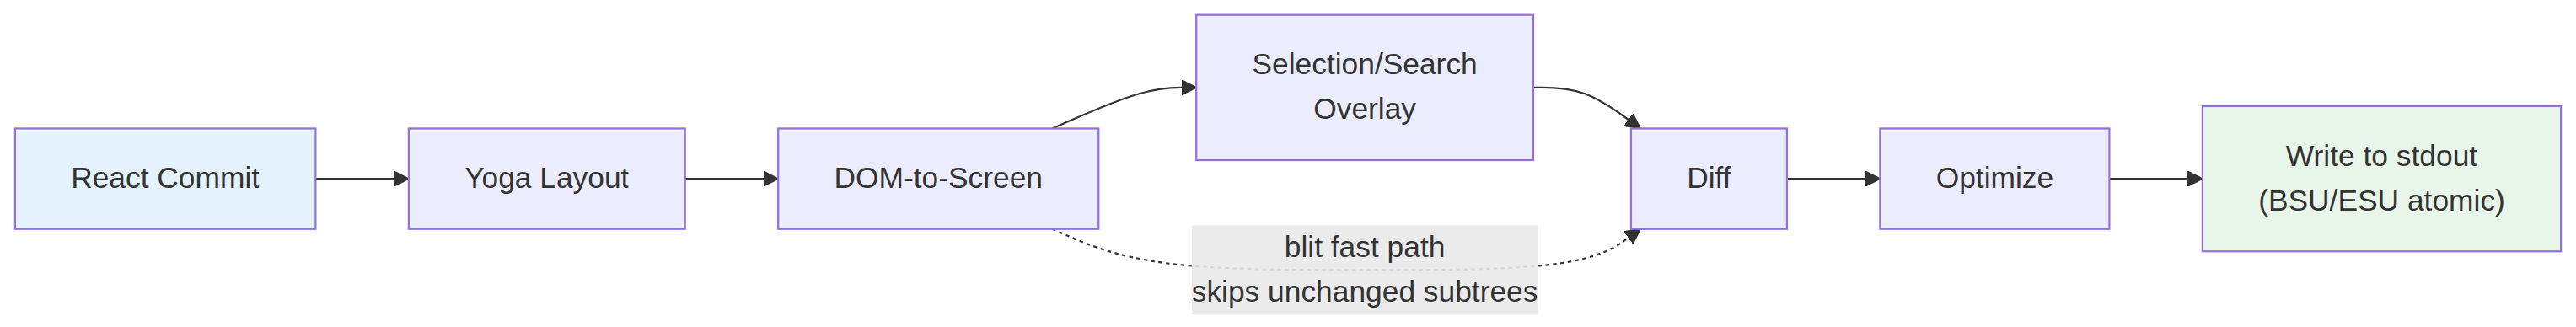
\includegraphics[width=14.41in,height=1.84in]{book/ch13-terminal-ui_files/figure-latex/mermaid-figure-1.png}

Each stage is timed individually and reported in
\texttt{FrameEvent.phases}. This per-stage instrumentation is essential
for diagnosing performance issues: when a frame takes 30ms, you need to
know whether the bottleneck is Yoga re-measuring text (stage 2), the
renderer walking a large dirty subtree (stage 3), or stdout backpressure
from a slow terminal (stage 7). The answer determines the fix.

\textbf{Stage 1: React commit and Yoga layout.} The reconciler processes
state updates and calls \texttt{resetAfterCommit}. This sets the root
node's width to \texttt{terminalColumns} and runs
\texttt{yogaNode.calculateLayout()}. Yoga computes the entire flexbox
tree in one pass, following the CSS flexbox specification: it resolves
flex-grow, flex-shrink, padding, margin, gap, alignment, and wrapping
across all nodes. The results -- \texttt{getComputedWidth()},
\texttt{getComputedHeight()}, \texttt{getComputedLeft()},
\texttt{getComputedTop()} -- are cached per node. For \texttt{ink-text}
nodes, Yoga calls the custom measure function (\texttt{measureTextNode})
during layout, which computes text dimensions via word wrapping and
grapheme measurement. This is the most expensive per-node operation: it
must handle Unicode grapheme clusters, CJK double-width characters,
emoji sequences, and ANSI escape codes embedded in text content.

\textbf{Stage 2: DOM-to-screen.} The renderer walks the DOM tree
depth-first, writing characters and styles into a \texttt{Screen}
buffer. Each character becomes a packed cell. The output is a complete
frame: every cell on the terminal has a defined character, style, and
width.

\textbf{Stage 3: Overlay.} Text selection and search highlighting modify
the screen buffer in-place, flipping style IDs on matching cells.
Selection applies inverse video to create the familiar ``highlighted
text'' appearance. Search highlighting applies a more aggressive visual
treatment: inverse + yellow foreground + bold + underline for the
current match, inverse only for other matches. This contaminates the
buffer -- tracked by a \texttt{prevFrameContaminated} flag so the next
frame knows to skip the blit fast-path. The contamination is a
deliberate tradeoff: modifying the buffer in-place avoids allocating a
separate overlay buffer (saving 48KB on a 200x120 terminal), at the cost
of one full-damage frame after the overlay is cleared.

\textbf{Stage 4: Diff.} The new screen is compared cell-by-cell against
the front frame's screen. Only changed cells produce output. The
comparison is two integer comparisons per cell (the two packed
\texttt{Int32} words), and the diff walks the damage rectangle rather
than the full screen. On a steady-state frame (only a spinner ticking),
this might produce patches for 3 cells out of 24,000. Each patch is a
\texttt{\{\ type:\ \textquotesingle{}stdout\textquotesingle{},\ content:\ string\ \}}
object containing the cursor-move sequence and the ANSI-encoded cell
content.

\textbf{Stage 5: Optimize.} Adjacent patches on the same row are merged
into a single write. Redundant cursor moves are eliminated -- if patch N
ends at column 10 and patch N+1 starts at column 11, the cursor is
already in the right position and no move sequence is needed. Style
transitions are pre-serialized via the \texttt{StylePool.transition()}
cache, so changing from ``bold red'' to ``dim green'' is a single cached
string lookup rather than a diff-and-serialize operation. The optimizer
typically reduces the byte count by 30-50\% compared to naive per-cell
output.

\textbf{Stage 6: Write.} The optimized patches are serialized to ANSI
escape sequences and written to stdout in a single \texttt{write()}
call, wrapped in synchronous update markers (BSU/ESU) on terminals that
support them. BSU (Begin Synchronized Update,
\texttt{ESC\ {[}\ ?\ 2026\ h}) tells the terminal to buffer all
following output, and ESU (\texttt{ESC\ {[}\ ?\ 2026\ l}) tells it to
flush. This eliminates visible tearing on terminals that support the
protocol -- the entire frame appears atomically.

Every frame reports its timing breakdown via a \texttt{FrameEvent}
object:

\begin{Shaded}
\begin{Highlighting}[]
\KeywordTok{interface}\NormalTok{ FrameEvent \{}
\NormalTok{  durationMs}\OperatorTok{:} \DataTypeTok{number}\OperatorTok{;}
\NormalTok{  phases}\OperatorTok{:}\NormalTok{ \{}
\NormalTok{    renderer}\OperatorTok{:} \DataTypeTok{number}\OperatorTok{;}    \CommentTok{// DOM{-}to{-}screen}
\NormalTok{    diff}\OperatorTok{:} \DataTypeTok{number}\OperatorTok{;}        \CommentTok{// Screen comparison}
\NormalTok{    optimize}\OperatorTok{:} \DataTypeTok{number}\OperatorTok{;}    \CommentTok{// Patch merging}
\NormalTok{    write}\OperatorTok{:} \DataTypeTok{number}\OperatorTok{;}       \CommentTok{// stdout write}
\NormalTok{    yoga}\OperatorTok{:} \DataTypeTok{number}\OperatorTok{;}        \CommentTok{// Layout computation}
\NormalTok{  \}}\OperatorTok{;}
\NormalTok{  yogaVisited}\OperatorTok{:} \DataTypeTok{number}\OperatorTok{;}   \CommentTok{// Nodes traversed}
\NormalTok{  yogaMeasured}\OperatorTok{:} \DataTypeTok{number}\OperatorTok{;}  \CommentTok{// Nodes that ran measure()}
\NormalTok{  yogaCacheHits}\OperatorTok{:} \DataTypeTok{number}\OperatorTok{;} \CommentTok{// Nodes with cached layout}
\NormalTok{  flickers}\OperatorTok{:}\NormalTok{ FlickerEvent[]}\OperatorTok{;}  \CommentTok{// Full{-}reset attributions}
\NormalTok{\}}
\end{Highlighting}
\end{Shaded}

When \texttt{CLAUDE\_CODE\_DEBUG\_REPAINTS} is enabled, full-screen
resets are attributed to their source React component via
\texttt{findOwnerChainAtRow()}. This is the terminal equivalent of React
DevTools' ``Highlight Updates'' -- it shows you which component caused
the entire screen to repaint, which is the most expensive thing that can
happen in the rendering pipeline.

The blit optimization deserves special attention. When a node is not
dirty and its position has not changed since the previous frame (checked
via a node cache), the renderer copies cells directly from
\texttt{prevScreen} to the current screen instead of re-rendering the
subtree. This makes steady-state frames extremely cheap -- on a typical
frame where only a spinner is ticking, the blit covers 99\% of the
screen and only the spinner's 3-4 cells are re-rendered from scratch.

The blit is disabled under three conditions:

\begin{enumerate}
\def\labelenumi{\arabic{enumi}.}
\tightlist
\item
  \textbf{\texttt{prevFrameContaminated} is true} -- the selection
  overlay or a search highlight modified the front frame's screen buffer
  in-place, so those cells cannot be trusted as the ``correct'' previous
  state
\item
  \textbf{An absolute-positioned node was removed} -- absolute
  positioning means the node could have painted over non-sibling cells,
  and those cells need to be re-rendered from the elements that actually
  own them
\item
  \textbf{Layout shifted} -- any node's cached position differs from its
  current computed position, meaning the blit would copy cells to the
  wrong coordinates
\end{enumerate}

The damage rectangle (\texttt{screen.damage}) tracks the bounding box of
all written cells during rendering. The diff only examines rows within
this rectangle, skipping entirely unchanged regions. On a 120-row
terminal where a streaming message occupies rows 80-100, the diff checks
20 rows instead of 120 -- a 6x reduction in comparison work.

\begin{center}\rule{0.5\linewidth}{0.5pt}\end{center}

\section{Double-Buffer Rendering and Frame
Scheduling}\label{double-buffer-rendering-and-frame-scheduling}

The Ink class maintains two frame buffers:

\begin{Shaded}
\begin{Highlighting}[]
\KeywordTok{private}\NormalTok{ frontFrame}\OperatorTok{:}\NormalTok{ Frame}\OperatorTok{;}  \CommentTok{// Currently displayed on terminal}
\KeywordTok{private}\NormalTok{ backFrame}\OperatorTok{:}\NormalTok{ Frame}\OperatorTok{;}   \CommentTok{// Being rendered into}
\end{Highlighting}
\end{Shaded}

Each \texttt{Frame} contains:

\begin{itemize}
\tightlist
\item
  \texttt{screen:\ Screen} -- the cell buffer (packed
  \texttt{Int32Array})
\item
  \texttt{viewport:\ Size} -- terminal dimensions at render time
\item
  \texttt{cursor:\ \{\ x,\ y,\ visible\ \}} -- where to park the
  terminal cursor
\item
  \texttt{scrollHint} -- DECSTBM (scroll region) optimization hint for
  alt-screen mode
\item
  \texttt{scrollDrainPending} -- whether a ScrollBox has remaining
  scroll delta to process
\end{itemize}

After each render, the frames swap:
\texttt{backFrame\ =\ frontFrame;\ frontFrame\ =\ newFrame}. The old
front frame becomes the next back frame, providing the
\texttt{prevScreen} for blit optimization and the baseline for
cell-level diffing.

This double-buffer design eliminates allocation. Instead of creating a
new \texttt{Screen} every frame, the renderer reuses the back frame's
buffer. The swap is a pointer assignment. The pattern is borrowed from
graphics programming, where double buffering prevents tearing by
ensuring the display reads from a complete frame while the renderer
writes to the other. In the terminal context, tearing is not the concern
(the BSU/ESU protocol handles that); the concern is GC pressure from
allocating and discarding \texttt{Screen} objects containing 48KB+ of
typed arrays every 16ms.

Render scheduling uses lodash \texttt{throttle} at 16ms (approximately
60fps), with leading and trailing edges enabled:

\begin{Shaded}
\begin{Highlighting}[]
\KeywordTok{const}\NormalTok{ deferredRender }\OperatorTok{=}\NormalTok{ () }\KeywordTok{=\textgreater{}} \FunctionTok{queueMicrotask}\NormalTok{(}\KeywordTok{this}\OperatorTok{.}\AttributeTok{onRender}\NormalTok{)}\OperatorTok{;}
\KeywordTok{this}\OperatorTok{.}\AttributeTok{scheduleRender} \OperatorTok{=} \FunctionTok{throttle}\NormalTok{(deferredRender}\OperatorTok{,}\NormalTok{ FRAME\_INTERVAL\_MS}\OperatorTok{,}\NormalTok{ \{}
\NormalTok{  leading}\OperatorTok{:} \KeywordTok{true}\OperatorTok{,}
\NormalTok{  trailing}\OperatorTok{:} \KeywordTok{true}\OperatorTok{,}
\NormalTok{\})}\OperatorTok{;}
\end{Highlighting}
\end{Shaded}

The microtask deferral is not accidental. \texttt{resetAfterCommit} runs
before React's layout effects phase. If the renderer ran synchronously
here, it would miss cursor declarations set in \texttt{useLayoutEffect}.
The microtask runs after layout effects but within the same event-loop
tick -- the terminal sees a single, consistent frame.

For scroll operations, a separate \texttt{setTimeout} at 4ms
(FRAME\_INTERVAL\_MS \textgreater\textgreater{} 2) provides faster
scroll frames without interfering with the throttle. Scroll mutations
bypass React entirely: \texttt{ScrollBox.scrollBy()} mutates DOM node
properties directly, calls \texttt{markDirty()}, and schedules a render
via microtask. No React state update, no reconciliation overhead, no
re-rendering of the entire message list for a single wheel event.

\textbf{Resize handling} is synchronous, not debounced. When the
terminal resizes, \texttt{handleResize} updates dimensions immediately
to keep layout consistent. For alt-screen mode, it resets frame buffers
and defers \texttt{ERASE\_SCREEN} into the next atomic BSU/ESU paint
block rather than writing it immediately. Writing the erase
synchronously would leave the screen blank for the \textasciitilde80ms
the render takes; deferring it into the atomic block means old content
stays visible until the new frame is fully ready.

\textbf{Alt-screen management} adds another layer. The
\texttt{AlternateScreen} component enters DEC 1049 alternate screen
buffer on mount, constraining height to terminal rows. It uses
\texttt{useInsertionEffect} -- not \texttt{useLayoutEffect} -- to ensure
the \texttt{ENTER\_ALT\_SCREEN} escape sequence reaches the terminal
before the first render frame. Using \texttt{useLayoutEffect} would be
too late: the first frame would render to the main screen buffer,
producing a visible flash before the switch. \texttt{useInsertionEffect}
runs before layout effects and before the browser (or terminal) would
paint, making the transition seamless.

\begin{center}\rule{0.5\linewidth}{0.5pt}\end{center}

\section{Pool-Based Memory: Why Interning
Matters}\label{pool-based-memory-why-interning-matters}

A 200-column by 120-row terminal has 24,000 cells. If each cell were a
JavaScript object with a \texttt{char} string, a \texttt{style} string,
and a \texttt{hyperlink} string, that is 72,000 string allocations per
frame -- plus 24,000 object allocations for the cells themselves. At
60fps, that is 5.76 million allocations per second. V8's garbage
collector can handle this, but not without pauses that show up as
dropped frames. The GC pauses are typically 1-5ms, but they are
unpredictable: they might hit during a streaming token update, causing a
visible stutter exactly when the user is watching the output.

Claude Code eliminates this entirely with packed typed arrays and three
interning pools. The result: zero per-frame object allocations for the
cell buffer. The only allocations are in the pools themselves
(amortized, since most characters and styles are interned on the first
frame and reused thereafter) and in the patch strings produced by the
diff (unavoidable, since stdout.write requires string or Buffer
arguments).

\textbf{The cell layout} uses two \texttt{Int32} words per cell, stored
in a contiguous \texttt{Int32Array}:

\begin{verbatim}
word0: charId        (32 bits, index into CharPool)
word1: styleId[31:17] | hyperlinkId[16:2] | width[1:0]
\end{verbatim}

A parallel \texttt{BigInt64Array} view over the same buffer enables bulk
operations -- clearing a row is a single \texttt{fill()} call on 64-bit
words instead of zeroing individual fields.

\textbf{CharPool} interns character strings to integer IDs. It has a
fast path for ASCII: a 128-entry \texttt{Int32Array} maps character
codes directly to pool indices, avoiding the \texttt{Map} lookup
entirely. Multi-byte characters (emoji, CJK ideographs) fall through to
a \texttt{Map\textless{}string,\ number\textgreater{}}. Index 0 is
always space, index 1 is always empty string.

\begin{Shaded}
\begin{Highlighting}[]
\ImportTok{export} \KeywordTok{class}\NormalTok{ CharPool \{}
  \KeywordTok{private}\NormalTok{ strings}\OperatorTok{:} \DataTypeTok{string}\NormalTok{[] }\OperatorTok{=}\NormalTok{ [}\StringTok{\textquotesingle{} \textquotesingle{}}\OperatorTok{,} \StringTok{\textquotesingle{}\textquotesingle{}}\NormalTok{]}
  \KeywordTok{private}\NormalTok{ ascii}\OperatorTok{:} \BuiltInTok{Int32Array} \OperatorTok{=} \FunctionTok{initCharAscii}\NormalTok{()}

  \FunctionTok{intern}\NormalTok{(char}\OperatorTok{:} \DataTypeTok{string}\NormalTok{)}\OperatorTok{:} \DataTypeTok{number}\NormalTok{ \{}
    \ControlFlowTok{if}\NormalTok{ (char}\OperatorTok{.}\AttributeTok{length} \OperatorTok{===} \DecValTok{1}\NormalTok{) \{}
      \KeywordTok{const}\NormalTok{ code }\OperatorTok{=}\NormalTok{ char}\OperatorTok{.}\FunctionTok{charCodeAt}\NormalTok{(}\DecValTok{0}\NormalTok{)}
      \ControlFlowTok{if}\NormalTok{ (code }\OperatorTok{\textless{}} \DecValTok{128}\NormalTok{) \{}
        \KeywordTok{const}\NormalTok{ cached }\OperatorTok{=} \KeywordTok{this}\OperatorTok{.}\AttributeTok{ascii}\NormalTok{[code]}\OperatorTok{!}
        \ControlFlowTok{if}\NormalTok{ (cached }\OperatorTok{!==} \OperatorTok{{-}}\DecValTok{1}\NormalTok{) }\ControlFlowTok{return}\NormalTok{ cached}
        \KeywordTok{const}\NormalTok{ index }\OperatorTok{=} \KeywordTok{this}\OperatorTok{.}\AttributeTok{strings}\OperatorTok{.}\AttributeTok{length}
        \KeywordTok{this}\OperatorTok{.}\AttributeTok{strings}\OperatorTok{.}\FunctionTok{push}\NormalTok{(char)}
        \KeywordTok{this}\OperatorTok{.}\AttributeTok{ascii}\NormalTok{[code] }\OperatorTok{=}\NormalTok{ index}
        \ControlFlowTok{return}\NormalTok{ index}
\NormalTok{      \}}
\NormalTok{    \}}
    \CommentTok{// Map fallback for multi{-}byte characters}
    \OperatorTok{...}
\NormalTok{  \}}
\NormalTok{\}}
\end{Highlighting}
\end{Shaded}

\textbf{StylePool} interns arrays of ANSI style codes to integer IDs.
The clever part: bit 0 of each ID encodes whether the style has a
visible effect on space characters (background color, inverse,
underline). Foreground-only styles get even IDs; styles visible on
spaces get odd IDs. This lets the renderer skip invisible spaces with a
single bitmask check --
\texttt{if\ (!(styleId\ \&\ 1)\ \&\&\ charId\ ===\ 0)\ continue} --
without looking up the style definition. The pool also caches
pre-serialized ANSI transition strings between any two style IDs, so
transitioning from ``bold red'' to ``dim green'' is a cached string
concatenation, not a diff-and-serialize operation.

\textbf{HyperlinkPool} interns OSC 8 hyperlink URIs. Index 0 means no
hyperlink.

All three pools are shared across the front and back frames. This is a
critical design decision. Because the pools are shared, interned IDs are
valid across frames: the blit optimization can copy packed cell words
directly from \texttt{prevScreen} to the current screen without
re-interning. The diff can compare IDs as integers without string
lookups. If each frame had its own pools, the blit would need to
re-intern every copied cell (looking up the string by old ID, then
interning it in the new pool), which would negate most of the blit's
performance benefit.

Pools are periodically reset (every 5 minutes) to prevent unbounded
growth during long sessions. A migration pass re-interns the front
frame's live cells into the fresh pools.

\textbf{CellWidth} handles double-wide characters with a 2-bit
classification:

\begin{longtable}[]{@{}ll@{}}
\toprule\noalign{}
Value & Meaning \\
\midrule\noalign{}
\endhead
\bottomrule\noalign{}
\endlastfoot
0 (Narrow) & Standard single-column character \\
1 (Wide) & CJK/emoji head cell, occupies two columns \\
2 (SpacerTail) & Second column of a wide character \\
3 (SpacerHead) & Soft-wrap continuation marker \\
\end{longtable}

This is stored in the low 2 bits of \texttt{word1}, making width checks
on packed cells free -- no field extraction needed for the common case.

Additional per-cell metadata lives in parallel arrays rather than the
packed cells:

\begin{itemize}
\tightlist
\item
  \textbf{\texttt{noSelect:\ Uint8Array}} -- per-cell flag excluding
  content from text selection. Used for UI chrome (borders, indicators)
  that should not appear in copied text
\item
  \textbf{\texttt{softWrap:\ Int32Array}} -- per-row marker indicating
  word-wrap continuation. When the user selects text across a
  soft-wrapped line, the selection logic knows not to insert a newline
  at the wrap point
\item
  \textbf{\texttt{damage:\ Rectangle}} -- bounding box of all written
  cells in the current frame. The diff only examines rows within this
  rectangle, skipping entirely unchanged regions
\end{itemize}

These parallel arrays avoid widening the packed cell format (which would
increase cache pressure in the diff inner loop) while providing the
metadata that selection, copy, and optimization need.

The \texttt{Screen} also exposes a \texttt{createScreen()} factory that
takes dimensions and pool references. Creating a screen zeroes the
\texttt{Int32Array} via \texttt{fill(0n)} on the \texttt{BigInt64Array}
view -- a single native call that clears the entire buffer in
microseconds. This is used during resize (when new frame buffers are
needed) and during pool migration (when the old screen's cells are
re-interned into fresh pools).

\begin{center}\rule{0.5\linewidth}{0.5pt}\end{center}

\section{The REPL Component}\label{the-repl-component}

The REPL (\texttt{REPL.tsx}) is approximately 5,000 lines. It is the
largest single component in the codebase, and for good reason: it is the
orchestrator of the entire interactive experience. Everything flows
through it.

The component is organized into roughly nine sections:

\begin{enumerate}
\def\labelenumi{\arabic{enumi}.}
\tightlist
\item
  \textbf{Imports} (\textasciitilde100 lines) -- pulls in bootstrap
  state, commands, history, hooks, components, keybindings, cost
  tracking, notifications, swarm/team support, voice integration
\item
  \textbf{Feature-flagged imports} -- conditional loading of voice
  integration, proactive mode, brief tool, and coordinator agent via
  \texttt{feature()} guards with \texttt{require()}
\item
  \textbf{State management} -- extensive \texttt{useState} calls
  covering messages, input mode, pending permissions, dialogs, cost
  thresholds, session state, tool state, and agent state
\item
  \textbf{QueryGuard} -- manages active API call lifecycle, preventing
  concurrent requests from stepping on each other
\item
  \textbf{Message handling} -- processes incoming messages from the
  query loop, normalizes ordering, manages streaming state
\item
  \textbf{Tool permission flow} -- coordinates permission requests
  between tool use blocks and the PermissionRequest dialog
\item
  \textbf{Session management} -- resume, switch, export conversations
\item
  \textbf{Keybinding setup} -- wires the keybinding providers:
  \texttt{KeybindingSetup}, \texttt{GlobalKeybindingHandlers},
  \texttt{CommandKeybindingHandlers}
\item
  \textbf{Render tree} -- composes the final UI from all the above
\end{enumerate}

Its render tree composes the full interface in fullscreen mode:

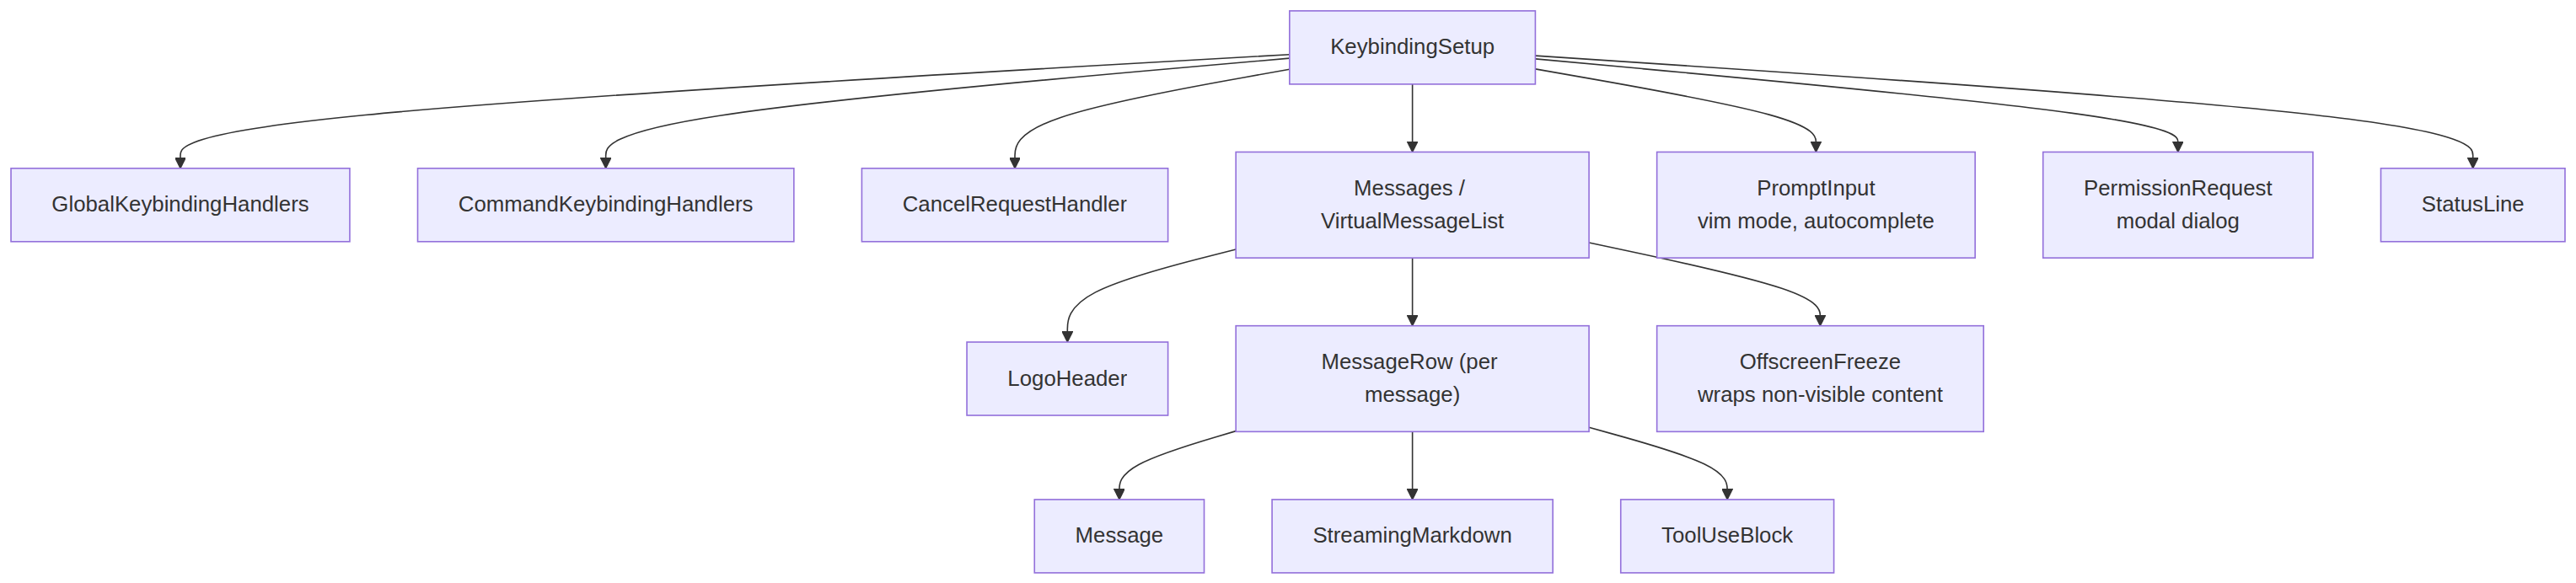
\includegraphics[width=19.76in,height=4.48in]{book/ch13-terminal-ui_files/figure-latex/mermaid-figure-2.png}

\texttt{OffscreenFreeze} is a performance optimization specific to
terminal rendering. When a message scrolls above the viewport, its React
element is cached and its subtree is frozen. This prevents timer-based
updates (spinners, elapsed time counters) in off-screen messages from
triggering terminal resets. Without this, a spinning indicator in
message 3 would cause a full repaint even though the user is looking at
message 47.

The component is compiled by the React Compiler throughout. Instead of
manual \texttt{useMemo} and \texttt{useCallback}, the compiler inserts
per-expression memoization using slot arrays:

\begin{Shaded}
\begin{Highlighting}[]
\KeywordTok{const}\NormalTok{ $ }\OperatorTok{=} \FunctionTok{\_c}\NormalTok{(}\DecValTok{14}\NormalTok{)}\OperatorTok{;}  \CommentTok{// 14 memoization slots}
\KeywordTok{let}\NormalTok{ t0}\OperatorTok{;}
\ControlFlowTok{if}\NormalTok{ ($[}\DecValTok{0}\NormalTok{] }\OperatorTok{!==}\NormalTok{ dep1 }\OperatorTok{||}\NormalTok{ $[}\DecValTok{1}\NormalTok{] }\OperatorTok{!==}\NormalTok{ dep2) \{}
\NormalTok{  t0 }\OperatorTok{=} \FunctionTok{expensiveComputation}\NormalTok{(dep1}\OperatorTok{,}\NormalTok{ dep2)}\OperatorTok{;}
\NormalTok{  $[}\DecValTok{0}\NormalTok{] }\OperatorTok{=}\NormalTok{ dep1}\OperatorTok{;}\NormalTok{ $[}\DecValTok{1}\NormalTok{] }\OperatorTok{=}\NormalTok{ dep2}\OperatorTok{;}\NormalTok{ $[}\DecValTok{2}\NormalTok{] }\OperatorTok{=}\NormalTok{ t0}\OperatorTok{;}
\NormalTok{\} }\ControlFlowTok{else}\NormalTok{ \{}
\NormalTok{  t0 }\OperatorTok{=}\NormalTok{ $[}\DecValTok{2}\NormalTok{]}\OperatorTok{;}
\NormalTok{\}}
\end{Highlighting}
\end{Shaded}

This pattern appears in every component in the codebase. It provides
finer granularity than \texttt{useMemo} (which memoizes at the hook
level) -- individual expressions within a render function get their own
dependency tracking and caching. For a 5,000-line component like the
REPL, this eliminates hundreds of potential unnecessary recomputations
per render.

\begin{center}\rule{0.5\linewidth}{0.5pt}\end{center}

\section{Selection and Search
Highlighting}\label{selection-and-search-highlighting}

Text selection and search highlighting operate as screen-buffer
overlays, applied after the main render but before the diff.

\textbf{Text selection} is alt-screen only. The Ink instance holds a
\texttt{SelectionState} tracking anchor and focus points, drag mode
(character/word/line), and captured rows that have scrolled off-screen.
When the user clicks and drags, the selection handler updates these
coordinates. During \texttt{onRender}, \texttt{applySelectionOverlay}
walks the affected rows and modifies cell style IDs in-place using
\texttt{StylePool.withSelectionBg()}, which returns a new style ID with
inverse video added. This direct mutation of the screen buffer is why
the \texttt{prevFrameContaminated} flag exists -- the front frame's
buffer has been modified by the overlay, so the next frame cannot trust
it for blit optimization and must do a full-damage diff.

Mouse tracking uses SGR 1003 mode, which reports clicks, drags, and
motion with column/row coordinates. The \texttt{App} component
implements multi-click detection: double-click selects a word,
triple-click selects a line. The detection uses a 500ms timeout and
1-cell position tolerance (the mouse can move one cell between clicks
without resetting the multi-click counter). Hyperlink clicks are
intentionally deferred by this timeout -- double-clicking a link selects
the word instead of opening the browser, matching the behavior users
expect from text editors.

A lost-release recovery mechanism handles the case where the user starts
a drag inside the terminal, moves the mouse outside the window, and
releases. The terminal reports the press and the drag, but not the
release (which happened outside its window). Without recovery, the
selection would be stuck in drag mode permanently. The recovery works by
detecting mouse motion events with no buttons pressed -- if we are in a
drag state and receive a no-button motion event, we infer that the
button was released outside the window and finalize the selection.

\textbf{Search highlighting} has two mechanisms running in parallel. The
scan-based path (\texttt{applySearchHighlight}) walks visible cells
looking for the query string and applies SGR inverse styling. The
position-based path uses pre-computed \texttt{MatchPosition{[}{]}} from
\texttt{scanElementSubtree()}, stored message-relative, and applies them
at known offsets with a ``current match'' yellow highlight using stacked
ANSI codes (inverse + yellow foreground + bold + underline). The yellow
foreground combined with inverse becomes a yellow background -- the
terminal swaps fg/bg when inverse is active. The underline is the
fallback visibility marker for themes where the yellow clashes with
existing background colors.

\textbf{Cursor declaration} solves a subtle problem. Terminal emulators
render IME (Input Method Editor) preedit text at the physical cursor
position. CJK users composing characters need the cursor to be at the
text input's caret, not at the bottom of the screen where the terminal
would naturally park it. The \texttt{useDeclaredCursor} hook lets a
component declare where the cursor should be after each frame. The Ink
class reads the declared node's position from \texttt{nodeCache},
translates it to screen coordinates, and emits cursor-move sequences
after the diff. Screen readers and magnifiers also track the physical
cursor, so this mechanism benefits accessibility as well as CJK input.

In main-screen mode, the declared cursor position is tracked separately
from \texttt{frame.cursor} (which must stay at the content bottom for
the log-update's relative-move invariants). In alt-screen mode, the
problem is simpler: every frame begins with \texttt{CSI\ H} (cursor
home), so the declared cursor is just an absolute position emitted at
the end of the frame.

\begin{center}\rule{0.5\linewidth}{0.5pt}\end{center}

\section{Streaming Markdown}\label{streaming-markdown}

Rendering LLM output is the most demanding task the terminal UI faces.
Tokens arrive one at a time, 10-50 per second, and each one changes the
content of a message that might contain code blocks, lists, bold text,
and inline code. The naive approach -- re-parse the entire message on
every token -- would be catastrophic at scale.

Claude Code uses three optimizations:

\textbf{Token caching.} A module-level LRU cache (500 entries) stores
\texttt{marked.lexer()} results keyed by content hash. The cache
survives React unmount/remount cycles during virtual scrolling. When a
user scrolls back to a previously visible message, the markdown tokens
are served from cache instead of re-parsed.

\textbf{Fast-path detection.} \texttt{hasMarkdownSyntax()} checks the
first 500 characters for markdown markers via a single regex. If no
syntax is found, it constructs a single-paragraph token directly,
bypassing the full GFM parser. This saves approximately 3ms per render
on plain-text messages -- which matters when you are rendering 60 frames
per second.

\textbf{Lazy syntax highlighting.} Code block highlighting is loaded via
React \texttt{Suspense}. The \texttt{MarkdownBody} component renders
immediately with \texttt{highlight=\{null\}} as a fallback, then
resolves asynchronously with the cli-highlight instance. The user sees
the code immediately (unstyled), then it pops into color a frame or two
later.

The streaming case adds a wrinkle. When tokens arrive from the model,
the markdown content grows incrementally. Re-parsing the entire content
on every token would be O(n\^{}2) over the course of a message. The
fast-path detection helps -- most streaming content is plain text
paragraphs, which bypass the parser entirely -- but for messages with
code blocks and lists, the LRU cache provides the real optimization. The
cache key is the content hash, so when 10 tokens arrive and only the
last paragraph changes, the cached parse result for the unchanged prefix
is reused. The markdown renderer only re-parses the tail that changed.

The \texttt{StreamingMarkdown} component is distinct from the static
\texttt{Markdown} component. It handles the case where the content is
still being generated: incomplete code fences (a
\texttt{\textasciigrave{}\textasciigrave{}\textasciigrave{}} without a
closing fence), partial bold markers, and truncated list items. The
streaming variant is more forgiving in its parsing -- it does not error
on unclosed syntax because the closing syntax has not arrived yet. When
the message finishes streaming, the component transitions to the static
\texttt{Markdown} renderer, which applies full GFM parsing with strict
syntax checking.

Syntax highlighting for code blocks is the most expensive per-element
operation in the rendering pipeline. A 100-line code block can take
50-100ms to highlight with cli-highlight. Loading the highlighting
library itself takes 200-300ms (it bundles grammar definitions for
dozens of languages). Both costs are hidden behind React
\texttt{Suspense}: the code block renders immediately as plain text, the
highlighting library loads asynchronously, and when it resolves, the
code block re-renders with colors. The user sees code instantly and
colors a moment later -- a much better experience than a 300ms blank
frame while the library loads.

\begin{center}\rule{0.5\linewidth}{0.5pt}\end{center}

\section{Apply This: Rendering Streaming Output
Efficiently}\label{apply-this-rendering-streaming-output-efficiently}

The terminal rendering pipeline is a case study in eliminating work.
Three principles drive the design:

\textbf{Intern everything.} If you have a value that appears in
thousands of cells -- a style, a character, a URL -- store it once and
reference it by integer ID. Integer comparison is one CPU instruction.
String comparison is a loop. When your inner loop runs 24,000 times per
frame at 60fps, the difference between \texttt{===} on integers and
\texttt{===} on strings is the difference between smooth scrolling and
visible lag.

\textbf{Diff at the right level.} Cell-level diffing sounds expensive --
24,000 comparisons per frame. But it is two integer comparisons per cell
(the packed words), and on a steady-state frame, the diff bails out of
most rows after checking the first cell. The alternative -- re-rendering
the entire screen and writing it to stdout -- would produce 100KB+ of
ANSI escape sequences per frame. The diff typically produces under 1KB.

\textbf{Separate the hot path from React.} Scroll events arrive at
mouse-input frequency (potentially hundreds per second). Routing each
one through React's reconciler -- state update, reconciliation, commit,
layout, render -- adds 5-10ms of latency per event. By mutating DOM
nodes directly and scheduling renders via microtask, the scroll path
stays under 1ms. React is involved only in the final paint, where it
would run anyway.

These principles apply to any streaming output system, not just
terminals. If you are building a web application that renders real-time
data -- a log viewer, a chat client, a monitoring dashboard -- the same
tradeoffs apply. Intern repeated values. Diff against the previous
frame. Keep the hot path out of your reactive framework.

A fourth principle, specific to long-running sessions: \textbf{clean up
periodically.} Claude Code's pools grow monotonically as new characters
and styles are interned. Over a multi-hour session, the pools could
accumulate thousands of entries that are no longer referenced by any
live cell. The 5-minute reset cycle bounds this growth: every 5 minutes,
fresh pools are created, the front frame's cells are migrated
(re-interned into the new pools), and the old pools become garbage. This
is a generational collection strategy, applied at the application level
because the JavaScript GC has no visibility into the semantic liveness
of pool entries.

The decision to use \texttt{Int32Array} over plain objects has a subtler
benefit beyond GC pressure: memory locality. When the diff compares
24,000 cells, it walks a contiguous typed array. Modern CPUs prefetch
sequential memory accesses, so the entire screen comparison runs within
the L1/L2 cache. An object-per-cell layout would scatter cells across
the heap, turning every comparison into a cache miss. The performance
difference is measurable: on a 200x120 screen, the typed-array diff
completes in under 0.5ms, while an equivalent object-based diff takes
3-5ms -- enough to blow the 16ms frame budget when combined with the
other pipeline stages.

A fifth principle applies to any system that renders into a fixed-size
grid: \textbf{track damage bounds.} The \texttt{damage} rectangle on
each screen records the bounding box of cells that were written during
rendering. The diff consults this rectangle and skips rows outside it
entirely. When a streaming message occupies the bottom 20 rows of a
120-row terminal, the diff examines 20 rows, not 120. Combined with the
blit optimization (which populates the damage rectangle only for
re-rendered regions, not blitted ones), this means the common case --
one message streaming while the rest of the conversation is static --
touches a fraction of the screen buffer.

The broader lesson: performance in a rendering system is not about
making any single operation fast. It is about eliminating operations
entirely. The blit eliminates re-rendering. The damage rectangle
eliminates diffing. The pool sharing eliminates re-interning. The packed
cells eliminate allocation. Each optimization removes an entire category
of work, and they stack multiplicatively.

To put numbers on it: a worst-case frame (everything dirty, no blit,
full-screen damage) on a 200x120 terminal takes approximately 12ms. A
best-case frame (one dirty node, blit everything else, 3-row damage
rectangle) takes under 1ms. The system spends most of its time in the
best case. The streaming token arrival triggers one dirty text node,
which dirties its ancestors up to the message container, which is
typically 10-30 rows of the screen. The blit handles the other 90-110
rows. The damage rectangle constrains the diff to the dirty region. The
pool lookups are integer operations. The steady-state cost of streaming
one token is dominated by Yoga layout (which re-measures the dirty text
node and its ancestors) and the markdown re-parse -- not by the
rendering pipeline itself.

\begin{center}\rule{0.5\linewidth}{0.5pt}\end{center}

\chapter{Chapter 14: Input and
Interaction}\label{chapter-14-input-and-interaction}

\section{Raw Bytes, Meaningful
Actions}\label{raw-bytes-meaningful-actions}

When you press Ctrl+X followed by Ctrl+K in Claude Code, the terminal
sends two byte sequences separated by perhaps 200 milliseconds. The
first is \texttt{0x18} (ASCII CAN). The second is \texttt{0x0B} (ASCII
VT). Neither of these bytes carries any inherent meaning beyond
``control character.'' The input system must recognize that these two
bytes, arriving in sequence within a timeout window, constitute the
chord \texttt{ctrl+x\ ctrl+k}, which maps to the action
\texttt{chat:killAgents}, which terminates all running sub-agents.

Between the raw bytes and the killed agents, six systems activate: a
tokenizer splits escape sequences, a parser classifies them across five
terminal protocols, a keybinding resolver matches the sequence against
context-specific bindings, a chord state machine manages the multi-key
sequence, a handler executes the action, and React batches the resulting
state updates into a single render.

The difficulty is not in any one of these systems. It is in the
combinatorial explosion of terminal diversity. iTerm2 sends Kitty
keyboard protocol sequences. macOS Terminal sends legacy VT220
sequences. Ghostty over SSH sends xterm modifyOtherKeys. tmux may eat,
transform, or passthrough any of these depending on its configuration.
Windows Terminal has its own quirks with VT mode. The input system must
produce correct \texttt{ParsedKey} objects from all of them, because a
user should not have to know which keyboard protocol their terminal
uses.

This chapter traces the path from raw bytes to meaningful actions across
that landscape.

The design philosophy is progressive enhancement with graceful
degradation. On a modern terminal with Kitty keyboard protocol support,
Claude Code gets full modifier detection (Ctrl+Shift+A is distinct from
Ctrl+A), super key reporting (Cmd shortcuts), and unambiguous key
identification. On a legacy terminal over SSH, it falls back to the best
available protocol, losing some modifier distinctions but keeping core
functionality intact. The user never sees an error message about their
terminal being unsupported. They might not be able to use
\texttt{ctrl+shift+f} for global search, but \texttt{ctrl+r} for history
search works everywhere.

\begin{center}\rule{0.5\linewidth}{0.5pt}\end{center}

\section{The Key Parsing Pipeline}\label{the-key-parsing-pipeline}

Input arrives as chunks of bytes on stdin. The pipeline processes them
in stages:

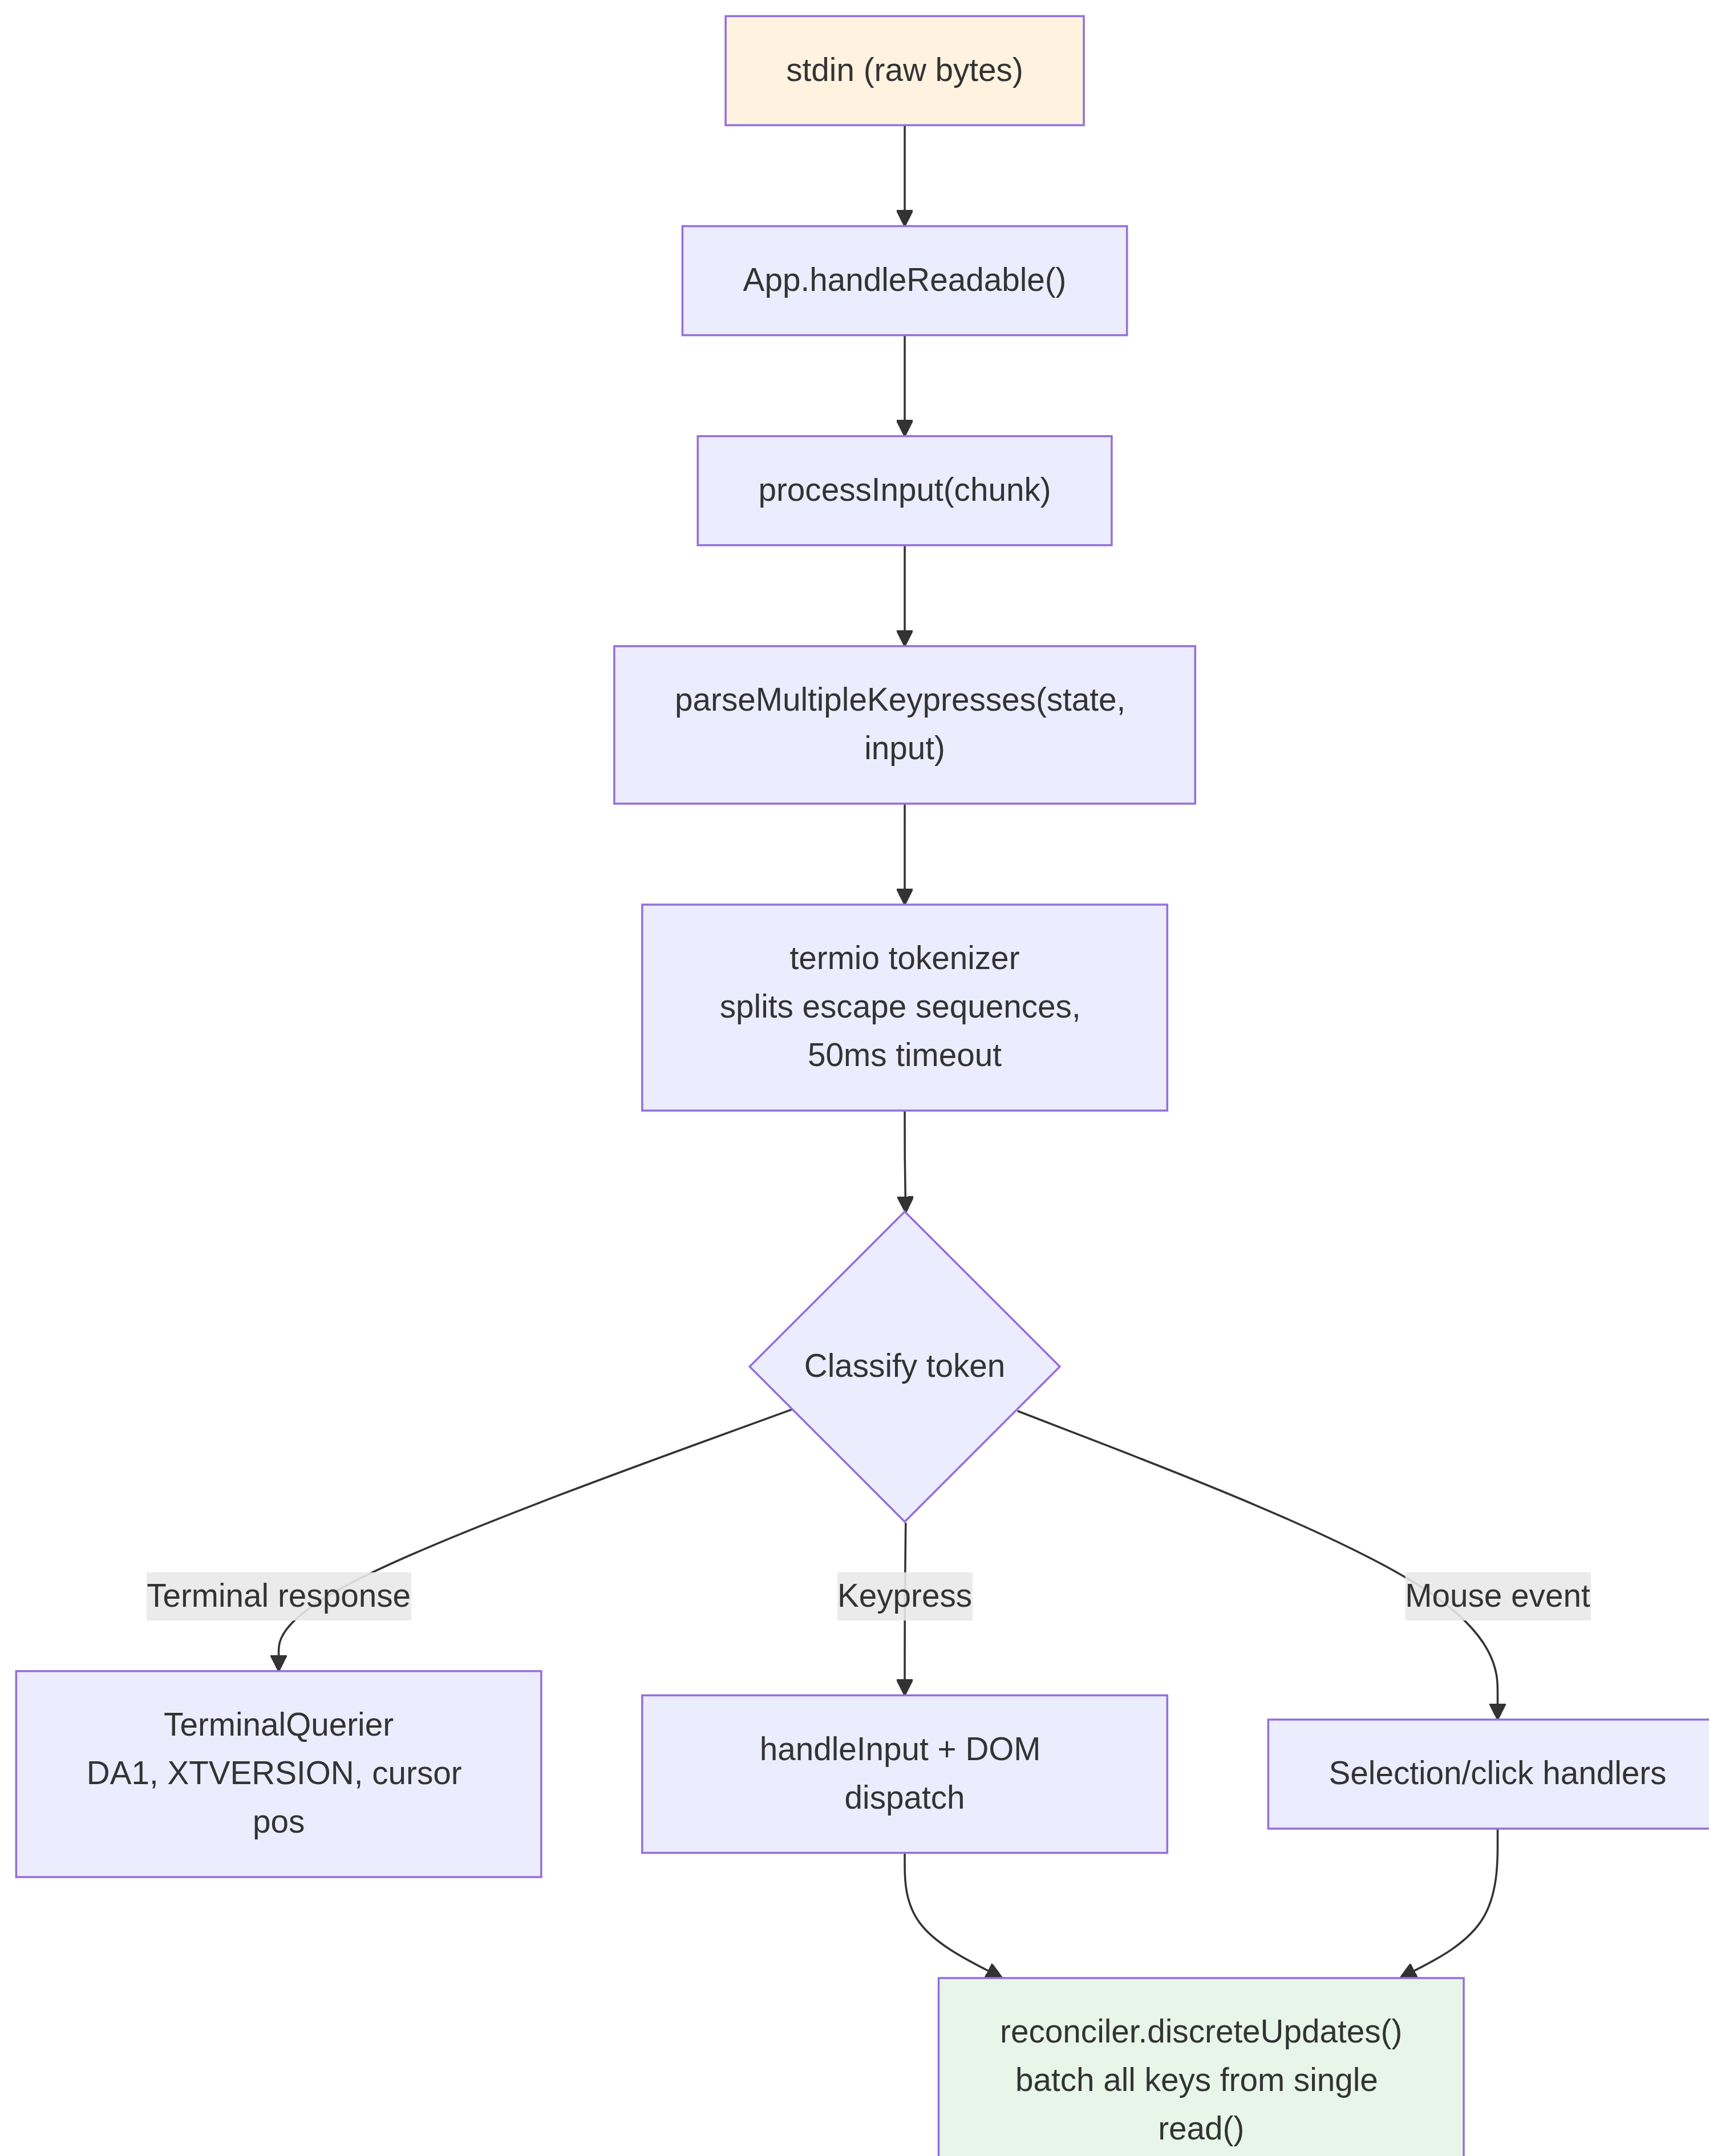
\includegraphics[width=8.99in,height=11.35in]{book/ch14-input-interaction_files/figure-latex/mermaid-figure-1.png}

The tokenizer is the foundation. Terminal input is a stream of bytes
that mixes printable characters, control codes, and multi-byte escape
sequences with no explicit framing. A single \texttt{read()} from stdin
might return \texttt{\textbackslash{}x1b{[}1;5A} (Ctrl+Up arrow), or it
might return \texttt{\textbackslash{}x1b} in one read and
\texttt{{[}1;5A} in the next, depending on how fast bytes arrive from
the PTY. The tokenizer maintains a state machine that buffers partial
escape sequences and emits complete tokens.

The incomplete-sequence problem is fundamental. When the tokenizer sees
a lone \texttt{\textbackslash{}x1b}, it cannot know whether this is the
Escape key or the start of a CSI sequence. It buffers the byte and
starts a 50ms timer. If no continuation arrives, the buffer is flushed
and the \texttt{\textbackslash{}x1b} becomes an Escape keypress. But
before flushing, the tokenizer checks \texttt{stdin.readableLength} --
if bytes are waiting in the kernel buffer, the timer re-arms rather than
flushing. This handles the case where the event loop was blocked past
50ms and the continuation bytes are already buffered but not yet read.

For paste operations, the timeout extends to 500ms. Pasted text can be
large and arrive in multiple chunks.

All parsed keys from a single \texttt{read()} are processed in one
\texttt{reconciler.discreteUpdates()} call. This batches React state
updates so that pasting 100 characters produces one re-render, not 100.
The batching is essential: without it, each character in a paste would
trigger a full reconciliation cycle -- state update, reconciliation,
commit, Yoga layout, render, diff, write. At 5ms per cycle, a
100-character paste would take 500ms to process. With batching, the same
paste takes one 5ms cycle.

\subsection{stdin Management}\label{stdin-management}

The \texttt{App} component manages raw mode via reference counting. When
any component needs raw input (the prompt, a dialog, vim mode), it calls
\texttt{setRawMode(true)}, incrementing a counter. When it no longer
needs raw input, it calls \texttt{setRawMode(false)}, decrementing. Raw
mode is only disabled when the counter reaches zero. This prevents a
common bug in terminal applications: component A enables raw mode,
component B enables raw mode, component A disables raw mode, and
suddenly component B's input breaks because raw mode was globally
disabled.

When raw mode is first enabled, the App:

\begin{enumerate}
\def\labelenumi{\arabic{enumi}.}
\tightlist
\item
  Stops early input capture (the bootstrap-phase mechanism that collects
  keystrokes before React mounts)
\item
  Puts stdin into raw mode (no line buffering, no echo, no signal
  processing)
\item
  Attaches a \texttt{readable} listener for async input processing
\item
  Enables bracketed paste (so pasted text is identifiable)
\item
  Enables focus reporting (so the app knows when the terminal window
  gains/loses focus)
\item
  Enables extended key reporting (Kitty keyboard protocol + xterm
  modifyOtherKeys)
\end{enumerate}

On disable, all of these are reversed in the opposite order. The careful
sequencing prevents escape sequence leaks -- disabling extended key
reporting before disabling raw mode ensures that the terminal does not
continue sending Kitty-encoded sequences after the app has stopped
parsing them.

The \texttt{onExit} signal handler (via the \texttt{signal-exit}
package) ensures cleanup happens even on unexpected termination. If the
process receives SIGTERM or SIGINT, the handler disables raw mode,
restores the terminal state, exits alternate screen if active, and
re-shows the cursor before the process exits. Without this cleanup, a
crashed Claude Code session would leave the terminal in raw mode with no
cursor and no echo -- the user would need to blindly type \texttt{reset}
to recover their terminal.

\begin{center}\rule{0.5\linewidth}{0.5pt}\end{center}

\section{Multi-Protocol Support}\label{multi-protocol-support}

Terminals do not agree on how to encode keyboard input. A modern
terminal emulator like Kitty sends structured sequences with full
modifier information. A legacy terminal over SSH sends ambiguous byte
sequences that require context to interpret. Claude Code's parser
handles five distinct protocols simultaneously, because the user's
terminal might be any of them.

\textbf{CSI u (Kitty keyboard protocol)} is the modern standard. Format:
\texttt{ESC\ {[}\ codepoint\ {[};\ modifier{]}\ u}. Example:
\texttt{ESC{[}13;2u} is Shift+Enter, \texttt{ESC{[}27u} is Escape with
no modifiers. The codepoint identifies the key unambiguously -- there is
no ambiguity between Escape-the-key and Escape-as-sequence-prefix. The
modifier word encodes shift, alt, ctrl, and super (Cmd) as individual
bits. Claude Code enables this protocol on terminals that support it via
the \texttt{ENABLE\_KITTY\_KEYBOARD} escape sequence at startup, and
disables it on exit via \texttt{DISABLE\_KITTY\_KEYBOARD}. The protocol
is detected through a query/response handshake: the application sends
\texttt{CSI\ ?\ u} and the terminal responds with
\texttt{CSI\ ?\ flags\ u}, where \texttt{flags} indicates the supported
protocol level.

\textbf{xterm modifyOtherKeys} is the fallback for terminals like
Ghostty over SSH, where the Kitty protocol is not negotiated. Format:
\texttt{ESC\ {[}\ 27\ ;\ modifier\ ;\ keycode\ \textasciitilde{}}. Note
that the parameter order is reversed from CSI u -- modifier comes before
keycode, then keycode. This is a common source of parser bugs. The
protocol is enabled via \texttt{CSI\ \textgreater{}\ 4\ ;\ 2\ m} and
emitted by Ghostty, tmux, and xterm when the terminal's TERM
identification is not detected (common over SSH where
\texttt{TERM\_PROGRAM} is not forwarded).

\textbf{Legacy terminal sequences} cover everything else: function keys
via \texttt{ESC\ O} and \texttt{ESC\ {[}} sequences, arrow keys, numpad,
Home/End/Insert/Delete, and the full zoo of VT100/VT220/xterm variations
accumulated over 40 years of terminal evolution. The parser uses two
regular expressions to match these: \texttt{FN\_KEY\_RE} for the
\texttt{ESC\ O/N/{[}/{[}{[}} prefix pattern (matching function keys,
arrow keys, and their modified variants), and
\texttt{META\_KEY\_CODE\_RE} for meta-key codes (\texttt{ESC} followed
by a single alphanumeric, the traditional Alt+key encoding).

The challenge with legacy sequences is ambiguity.
\texttt{ESC\ {[}\ 1\ ;\ 2\ R} could be Shift+F3 or a cursor position
report, depending on context. The parser resolves this with a
private-marker check: cursor position reports use
\texttt{CSI\ ?\ row\ ;\ col\ R} (with the \texttt{?} private marker),
while modified function keys use \texttt{CSI\ params\ R} (without it).
This disambiguation is why Claude Code requests DECXCPR (extended cursor
position reports) rather than standard CPR -- the extended form is
unambiguous.

Terminal identification adds another layer of complexity. On startup,
Claude Code sends an \texttt{XTVERSION} query
(\texttt{CSI\ \textgreater{}\ 0\ q}) to discover the terminal's name and
version. The response
(\texttt{DCS\ \textgreater{}\ \textbar{}\ name\ ST}) survives SSH
connections -- unlike \texttt{TERM\_PROGRAM}, which is an environment
variable that does not propagate through SSH. Knowing the terminal
identity allows the parser to handle terminal-specific quirks. For
example, xterm.js (used by VS Code's integrated terminal) has different
escape sequence behavior from native xterm, and the identification
string (\texttt{xterm.js(X.Y.Z)}) allows the parser to account for these
differences.

\textbf{SGR mouse events} use the format
\texttt{ESC\ {[}\ \textless{}\ button\ ;\ col\ ;\ row\ M/m}, where
\texttt{M} is press and \texttt{m} is release. Button codes encode the
action: 0/1/2 for left/middle/right click, 64/65 for wheel up/down (0x40
OR'd with a wheel bit), 32+ for drag (0x20 OR'd with a motion bit).
Wheel events are converted to \texttt{ParsedKey} objects so they flow
through the keybinding system; click and drag events become
\texttt{ParsedMouse} objects routed to the selection handler.

\textbf{Bracketed paste} wraps pasted content between
\texttt{ESC\ {[}200\textasciitilde{}} and
\texttt{ESC\ {[}201\textasciitilde{}} markers. Everything between the
markers becomes a single \texttt{ParsedKey} with
\texttt{isPasted:\ true}, regardless of what escape sequences the pasted
text might contain. This prevents pasted code from being interpreted as
commands -- a critical safety feature when a user pastes a code snippet
containing \texttt{\textbackslash{}x03} (which is Ctrl+C as a raw byte).

The output types from the parser form a clean discriminated union:

\begin{Shaded}
\begin{Highlighting}[]
\KeywordTok{type}\NormalTok{ ParsedKey }\OperatorTok{=}\NormalTok{ \{}
\NormalTok{  kind}\OperatorTok{:} \StringTok{\textquotesingle{}key\textquotesingle{}}\OperatorTok{;}
\NormalTok{  name}\OperatorTok{:} \DataTypeTok{string}\OperatorTok{;}        \CommentTok{// \textquotesingle{}return\textquotesingle{}, \textquotesingle{}escape\textquotesingle{}, \textquotesingle{}a\textquotesingle{}, \textquotesingle{}f1\textquotesingle{}, etc.}
\NormalTok{  ctrl}\OperatorTok{:} \DataTypeTok{boolean}\OperatorTok{;}\NormalTok{ meta}\OperatorTok{:} \DataTypeTok{boolean}\OperatorTok{;}\NormalTok{ shift}\OperatorTok{:} \DataTypeTok{boolean}\OperatorTok{;}
\NormalTok{  option}\OperatorTok{:} \DataTypeTok{boolean}\OperatorTok{;}\NormalTok{ super}\OperatorTok{:} \DataTypeTok{boolean}\OperatorTok{;}
\NormalTok{  sequence}\OperatorTok{:} \DataTypeTok{string}\OperatorTok{;}    \CommentTok{// Raw escape sequence for debugging}
\NormalTok{  isPasted}\OperatorTok{:} \DataTypeTok{boolean}\OperatorTok{;}   \CommentTok{// Inside bracketed paste}
\NormalTok{\}}

\KeywordTok{type}\NormalTok{ ParsedMouse }\OperatorTok{=}\NormalTok{ \{}
\NormalTok{  kind}\OperatorTok{:} \StringTok{\textquotesingle{}mouse\textquotesingle{}}\OperatorTok{;}
\NormalTok{  button}\OperatorTok{:} \DataTypeTok{number}\OperatorTok{;}      \CommentTok{// SGR button code}
\NormalTok{  action}\OperatorTok{:} \StringTok{\textquotesingle{}press\textquotesingle{}} \OperatorTok{|} \StringTok{\textquotesingle{}release\textquotesingle{}}\OperatorTok{;}
\NormalTok{  col}\OperatorTok{:} \DataTypeTok{number}\OperatorTok{;}\NormalTok{ row}\OperatorTok{:} \DataTypeTok{number}\OperatorTok{;}  \CommentTok{// 1{-}indexed terminal coordinates}
\NormalTok{\}}

\KeywordTok{type}\NormalTok{ ParsedResponse }\OperatorTok{=}\NormalTok{ \{}
\NormalTok{  kind}\OperatorTok{:} \StringTok{\textquotesingle{}response\textquotesingle{}}\OperatorTok{;}
\NormalTok{  response}\OperatorTok{:}\NormalTok{ TerminalResponse}\OperatorTok{;}  \CommentTok{// Routed to TerminalQuerier}
\NormalTok{\}}
\end{Highlighting}
\end{Shaded}

The \texttt{kind} discriminant ensures that downstream code handles each
input type explicitly. A key cannot be accidentally processed as a mouse
event; a terminal response cannot be accidentally interpreted as a
keypress. The \texttt{ParsedKey} type also carries the raw
\texttt{sequence} string for debugging -- when a user reports ``pressing
Ctrl+Shift+A does nothing,'' the debug log can show exactly what byte
sequence the terminal sent, making it possible to diagnose whether the
issue is in the terminal's encoding, the parser's recognition, or the
keybinding's configuration.

The \texttt{isPasted} flag on \texttt{ParsedKey} is critical for
security. When bracketed paste is enabled, the terminal wraps pasted
content in marker sequences. The parser sets \texttt{isPasted:\ true} on
the resulting key event, and the keybinding resolver skips keybinding
matching for pasted keys. Without this, pasting text containing
\texttt{\textbackslash{}x03} (Ctrl+C as a raw byte) or escape sequences
would trigger application commands. With it, pasted content is treated
as literal text input regardless of its byte content.

The parser also recognizes terminal responses -- sequences sent by the
terminal itself in answer to queries. These include device attributes
(DA1, DA2), cursor position reports, Kitty keyboard flag responses,
XTVERSION (terminal identification), and DECRPM (mode status). These are
routed to a \texttt{TerminalQuerier} rather than the input handler:

\begin{Shaded}
\begin{Highlighting}[]
\KeywordTok{type}\NormalTok{ TerminalResponse }\OperatorTok{=}
  \OperatorTok{|}\NormalTok{ \{ type}\OperatorTok{:} \StringTok{\textquotesingle{}decrpm\textquotesingle{}}\OperatorTok{;}\NormalTok{ mode}\OperatorTok{:} \DataTypeTok{number}\OperatorTok{;}\NormalTok{ status}\OperatorTok{:} \DataTypeTok{number}\NormalTok{ \}}
  \OperatorTok{|}\NormalTok{ \{ type}\OperatorTok{:} \StringTok{\textquotesingle{}da1\textquotesingle{}}\OperatorTok{;}\NormalTok{ params}\OperatorTok{:} \DataTypeTok{number}\NormalTok{[] \}}
  \OperatorTok{|}\NormalTok{ \{ type}\OperatorTok{:} \StringTok{\textquotesingle{}da2\textquotesingle{}}\OperatorTok{;}\NormalTok{ params}\OperatorTok{:} \DataTypeTok{number}\NormalTok{[] \}}
  \OperatorTok{|}\NormalTok{ \{ type}\OperatorTok{:} \StringTok{\textquotesingle{}kittyKeyboard\textquotesingle{}}\OperatorTok{;}\NormalTok{ flags}\OperatorTok{:} \DataTypeTok{number}\NormalTok{ \}}
  \OperatorTok{|}\NormalTok{ \{ type}\OperatorTok{:} \StringTok{\textquotesingle{}cursorPosition\textquotesingle{}}\OperatorTok{;}\NormalTok{ row}\OperatorTok{:} \DataTypeTok{number}\OperatorTok{;}\NormalTok{ col}\OperatorTok{:} \DataTypeTok{number}\NormalTok{ \}}
  \OperatorTok{|}\NormalTok{ \{ type}\OperatorTok{:} \StringTok{\textquotesingle{}osc\textquotesingle{}}\OperatorTok{;}\NormalTok{ code}\OperatorTok{:} \DataTypeTok{number}\OperatorTok{;}\NormalTok{ data}\OperatorTok{:} \DataTypeTok{string}\NormalTok{ \}}
  \OperatorTok{|}\NormalTok{ \{ type}\OperatorTok{:} \StringTok{\textquotesingle{}xtversion\textquotesingle{}}\OperatorTok{;}\NormalTok{ version}\OperatorTok{:} \DataTypeTok{string}\NormalTok{ \}}
\end{Highlighting}
\end{Shaded}

\textbf{Modifier decoding} follows the XTerm convention: the modifier
word is
\texttt{1\ +\ (shift\ ?\ 1\ :\ 0)\ +\ (alt\ ?\ 2\ :\ 0)\ +\ (ctrl\ ?\ 4\ :\ 0)\ +\ (super\ ?\ 8\ :\ 0)}.
The \texttt{meta} field in \texttt{ParsedKey} maps to Alt/Option (bit
2). The \texttt{super} field is distinct (bit 8, Cmd on macOS). This
distinction matters because Cmd shortcuts are reserved by the OS and
cannot be captured by terminal applications -- unless the terminal uses
the Kitty protocol, which reports super-modified keys that other
protocols silently swallow.

A stdin-gap detector triggers terminal mode re-assertion when no input
arrives for 5 seconds after a gap. This handles tmux reattach and laptop
wake scenarios, where the terminal's keyboard mode may have been reset
by the multiplexer or the OS. When re-assertion fires, it re-sends
\texttt{ENABLE\_KITTY\_KEYBOARD}, \texttt{ENABLE\_MODIFY\_OTHER\_KEYS},
bracketed paste, and focus reporting sequences. Without this, detaching
from a tmux session and reattaching would silently downgrade the
keyboard protocol to legacy mode, breaking modifier detection for the
rest of the session.

\subsection{The Terminal I/O Layer}\label{the-terminal-io-layer}

Beneath the parser sits a structured terminal I/O subsystem in
\texttt{ink/termio/}:

\begin{itemize}
\tightlist
\item
  \textbf{csi.ts} -- CSI (Control Sequence Introducer) sequences: cursor
  movement, erase, scroll regions, bracketed paste enable/disable, focus
  event enable/disable, Kitty keyboard protocol enable/disable
\item
  \textbf{dec.ts} -- DEC private mode sequences: alternate screen buffer
  (1049), mouse tracking modes (1000/1002/1003), cursor visibility,
  bracketed paste (2004), focus events (1004)
\item
  \textbf{osc.ts} -- Operating System Commands: clipboard access (OSC
  52), tab status, iTerm2 progress indicators, tmux/screen multiplexer
  wrapping (DCS passthrough for sequences that need to traverse a
  multiplexer boundary)
\item
  \textbf{sgr.ts} -- Select Graphic Rendition: the ANSI style code
  system (colors, bold, italic, underline, inverse)
\item
  \textbf{tokenize.ts} -- The stateful tokenizer for escape sequence
  boundary detection
\end{itemize}

The multiplexer wrapping deserves a note. When Claude Code runs inside
tmux, certain escape sequences (like Kitty keyboard protocol
negotiation) must pass through to the outer terminal. tmux uses DCS
passthrough (\texttt{ESC\ P\ ...\ ST}) to forward sequences it does not
understand. The \texttt{wrapForMultiplexer} function in \texttt{osc.ts}
detects the multiplexer environment and wraps sequences appropriately.
Without this, Kitty keyboard mode would silently fail inside tmux, and
the user would never know why their Ctrl+Shift bindings stopped working.

\subsection{The Event System}\label{the-event-system}

The \texttt{ink/events/} directory implements a browser-compatible event
system with seven event types: \texttt{KeyboardEvent},
\texttt{ClickEvent}, \texttt{FocusEvent}, \texttt{InputEvent},
\texttt{TerminalFocusEvent}, and base \texttt{TerminalEvent}. Each
carries \texttt{target}, \texttt{currentTarget}, \texttt{eventPhase},
and supports \texttt{stopPropagation()},
\texttt{stopImmediatePropagation()}, and \texttt{preventDefault()}.

The \texttt{InputEvent} wrapping \texttt{ParsedKey} exists for backward
compatibility with the legacy \texttt{EventEmitter} path, which older
components may still use. New components use the DOM-style keyboard
event dispatch with capture/bubble phases. Both paths fire from the same
parsed key, so they are always consistent -- a key that arrives on stdin
produces exactly one \texttt{ParsedKey}, which spawns both an
\texttt{InputEvent} (for legacy listeners) and a \texttt{KeyboardEvent}
(for DOM-style dispatch). This dual-path design allows incremental
migration from the EventEmitter pattern to the DOM event pattern without
breaking existing components.

\begin{center}\rule{0.5\linewidth}{0.5pt}\end{center}

\section{The Keybinding System}\label{the-keybinding-system}

The keybinding system separates three concerns that are often tangled
together: what key triggers what action (bindings), what happens when an
action fires (handlers), and which bindings are active right now
(contexts).

\subsection{Bindings: Declarative
Configuration}\label{bindings-declarative-configuration}

Default bindings are defined in \texttt{defaultBindings.ts} as an array
of \texttt{KeybindingBlock} objects, each scoped to a context:

\begin{Shaded}
\begin{Highlighting}[]
\ImportTok{export} \KeywordTok{const}\NormalTok{ DEFAULT\_BINDINGS}\OperatorTok{:}\NormalTok{ KeybindingBlock[] }\OperatorTok{=}\NormalTok{ [}
\NormalTok{  \{}
\NormalTok{    context}\OperatorTok{:} \StringTok{\textquotesingle{}Global\textquotesingle{}}\OperatorTok{,}
\NormalTok{    bindings}\OperatorTok{:}\NormalTok{ \{}
      \StringTok{\textquotesingle{}ctrl+c\textquotesingle{}}\OperatorTok{:} \StringTok{\textquotesingle{}app:interrupt\textquotesingle{}}\OperatorTok{,}
      \StringTok{\textquotesingle{}ctrl+d\textquotesingle{}}\OperatorTok{:} \StringTok{\textquotesingle{}app:exit\textquotesingle{}}\OperatorTok{,}
      \StringTok{\textquotesingle{}ctrl+l\textquotesingle{}}\OperatorTok{:} \StringTok{\textquotesingle{}app:redraw\textquotesingle{}}\OperatorTok{,}
      \StringTok{\textquotesingle{}ctrl+r\textquotesingle{}}\OperatorTok{:} \StringTok{\textquotesingle{}history:search\textquotesingle{}}\OperatorTok{,}
\NormalTok{    \}}\OperatorTok{,}
\NormalTok{  \}}\OperatorTok{,}
\NormalTok{  \{}
\NormalTok{    context}\OperatorTok{:} \StringTok{\textquotesingle{}Chat\textquotesingle{}}\OperatorTok{,}
\NormalTok{    bindings}\OperatorTok{:}\NormalTok{ \{}
      \StringTok{\textquotesingle{}escape\textquotesingle{}}\OperatorTok{:} \StringTok{\textquotesingle{}chat:cancel\textquotesingle{}}\OperatorTok{,}
      \StringTok{\textquotesingle{}ctrl+x ctrl+k\textquotesingle{}}\OperatorTok{:} \StringTok{\textquotesingle{}chat:killAgents\textquotesingle{}}\OperatorTok{,}
      \StringTok{\textquotesingle{}enter\textquotesingle{}}\OperatorTok{:} \StringTok{\textquotesingle{}chat:submit\textquotesingle{}}\OperatorTok{,}
      \StringTok{\textquotesingle{}up\textquotesingle{}}\OperatorTok{:} \StringTok{\textquotesingle{}history:previous\textquotesingle{}}\OperatorTok{,}
      \StringTok{\textquotesingle{}ctrl+x ctrl+e\textquotesingle{}}\OperatorTok{:} \StringTok{\textquotesingle{}chat:externalEditor\textquotesingle{}}\OperatorTok{,}
\NormalTok{    \}}\OperatorTok{,}
\NormalTok{  \}}\OperatorTok{,}
  \CommentTok{// ... 14 more contexts}
\NormalTok{]}
\end{Highlighting}
\end{Shaded}

Platform-specific bindings are handled at definition time. Image paste
is \texttt{ctrl+v} on macOS/Linux but \texttt{alt+v} on Windows (where
\texttt{ctrl+v} is system paste). Mode cycling is \texttt{shift+tab} on
terminals with VT mode support but \texttt{meta+m} on Windows Terminal
without it. Feature-flagged bindings (quick search, voice mode, terminal
panel) are conditionally included.

Users can override any binding via
\texttt{\textasciitilde{}/.claude/keybindings.json}. The parser accepts
modifier aliases (\texttt{ctrl}/\texttt{control},
\texttt{alt}/\texttt{opt}/\texttt{option},
\texttt{cmd}/\texttt{command}/\texttt{super}/\texttt{win}), key aliases
(\texttt{esc} -\textgreater{} \texttt{escape}, \texttt{return}
-\textgreater{} \texttt{enter}), chord notation (space-separated steps
like \texttt{ctrl+k\ ctrl+s}), and null actions to unbind default keys.
A null action is not the same as not defining a binding -- it explicitly
blocks the default binding from firing, which is important for users who
want to reclaim a key for their terminal's use.

\subsection{Contexts: 16 Scopes of
Activity}\label{contexts-16-scopes-of-activity}

Each context represents a mode of interaction where a specific set of
bindings applies:

\begin{longtable}[]{@{}ll@{}}
\toprule\noalign{}
Context & When Active \\
\midrule\noalign{}
\endhead
\bottomrule\noalign{}
\endlastfoot
Global & Always \\
Chat & Prompt input is focused \\
Autocomplete & Completion menu is visible \\
Confirmation & Permission dialog is showing \\
Scroll & Alt-screen with scrollable content \\
Transcript & Read-only transcript viewer \\
HistorySearch & Reverse history search (ctrl+r) \\
Task & A background task is running \\
Help & Help overlay is displayed \\
MessageSelector & Rewind dialog \\
MessageActions & Message cursor navigation \\
DiffDialog & Diff viewer \\
Select & Generic selection list \\
Settings & Config panel \\
Tabs & Tab navigation \\
Footer & Footer indicators \\
\end{longtable}

When a key arrives, the resolver builds a context list from the
currently active contexts (determined by React component state),
deduplicates it preserving priority order, and searches for a matching
binding. The last matching binding wins -- this is how user overrides
take precedence over defaults. The context list is rebuilt on every
keystroke (it is cheap: array concatenation and deduplication of at most
16 strings), so context changes take effect immediately without any
subscription or listener mechanism.

The context design handles a tricky interaction pattern: nested modals.
When a permission dialog appears during a running task, both
\texttt{Confirmation} and \texttt{Task} contexts might be active. The
\texttt{Confirmation} context takes priority (it is registered later in
the component tree), so \texttt{y} triggers ``approve'' rather than any
task-level binding. When the dialog closes, the \texttt{Confirmation}
context deactivates and \texttt{Task} bindings resume. This stacking
behavior emerges naturally from the context list's priority ordering --
no special modal-handling code is needed.

\subsection{Reserved Shortcuts}\label{reserved-shortcuts}

Not everything can be rebound. The system enforces three tiers of
reservation:

\textbf{Non-rebindable} (hardcoded behavior): \texttt{ctrl+c}
(interrupt/exit), \texttt{ctrl+d} (exit), \texttt{ctrl+m} (identical to
Enter in all terminals -- rebinding it would break Enter).

\textbf{Terminal-reserved} (warnings): \texttt{ctrl+z} (SIGTSTP),
\texttt{ctrl+\textbackslash{}} (SIGQUIT). These can technically be
bound, but the terminal will intercept them before the application sees
them in most configurations.

\textbf{macOS-reserved} (errors): \texttt{cmd+c}, \texttt{cmd+v},
\texttt{cmd+x}, \texttt{cmd+q}, \texttt{cmd+w}, \texttt{cmd+tab},
\texttt{cmd+space}. The OS intercepts these before they reach the
terminal. Binding them would create a shortcut that never fires.

\subsection{The Resolution Flow}\label{the-resolution-flow}

When a key arrives, the resolution path is:

\begin{enumerate}
\def\labelenumi{\arabic{enumi}.}
\tightlist
\item
  Build the context list: the component's registered active contexts
  plus Global, deduplicated with priority preserved
\item
  Call \texttt{resolveKeyWithChordState(input,\ key,\ contexts)} against
  the merged binding table
\item
  On \texttt{match}: clear any pending chord, call the handler,
  \texttt{stopImmediatePropagation()} on the event
\item
  On \texttt{chord\_started}: save the pending keystrokes, stop
  propagation, start the chord timeout
\item
  On \texttt{chord\_cancelled}: clear the pending chord, let the event
  fall through
\item
  On \texttt{unbound}: clear the chord -- this is an explicit unbinding
  (user set the action to \texttt{null}), so propagation is stopped but
  no handler runs
\item
  On \texttt{none}: fall through to other handlers
\end{enumerate}

The ``last wins'' resolution strategy means that if both the default
bindings and user bindings define \texttt{ctrl+k} in the \texttt{Chat}
context, the user's binding takes precedence. This is evaluated at match
time by iterating bindings in definition order and keeping the last
match, rather than building an override map at load time. The advantage:
context-specific overrides compose naturally. A user can override
\texttt{enter} in \texttt{Chat} without affecting \texttt{enter} in
\texttt{Confirmation}.

\begin{center}\rule{0.5\linewidth}{0.5pt}\end{center}

\section{Chord Support}\label{chord-support}

The \texttt{ctrl+x\ ctrl+k} binding is a chord: two keystrokes that
together form a single action. The resolver manages this with a state
machine.

When a key arrives:

\begin{enumerate}
\def\labelenumi{\arabic{enumi}.}
\tightlist
\item
  The resolver appends it to any pending chord prefix
\item
  It checks whether any binding's chord starts with this prefix. If so,
  it returns \texttt{chord\_started} and saves the pending keystrokes
\item
  If the full chord matches a binding exactly, it returns \texttt{match}
  and clears the pending state
\item
  If the chord prefix matches nothing, it returns
  \texttt{chord\_cancelled}
\end{enumerate}

A \texttt{ChordInterceptor} component intercepts all input during the
chord wait state. It has a 1000ms timeout -- if the second keystroke
does not arrive within a second, the chord is cancelled and the first
keystroke is discarded. The \texttt{KeybindingContext} provides a
\texttt{pendingChordRef} for synchronous access to the pending state,
avoiding React state update delays that could cause the second keystroke
to be processed before the first one's state update completes.

The chord design avoids shadowing readline editing keys. Without chords,
the keybinding for ``kill agents'' might be \texttt{ctrl+k} -- but that
is readline's ``kill to end of line,'' which users expect in a terminal
text input. By using \texttt{ctrl+x} as a prefix (matching readline's
own chord prefix convention), the system gets a namespace of bindings
that do not conflict with single-key editing shortcuts.

The implementation handles an edge case that most chord systems miss:
what happens when the user presses \texttt{ctrl+x} but then types a
character that is not part of any chord? Without careful handling, that
character would be swallowed -- the chord interceptor consumed the
input, the chord was cancelled, and the character is gone. Claude Code's
\texttt{ChordInterceptor} returns \texttt{chord\_cancelled} in this
case, which causes the pending input to be discarded but allows the
non-matching character to fall through to normal input processing. The
character is not lost; only the chord prefix is discarded. This matches
the behavior users expect from Emacs-style chord prefixes.

\begin{center}\rule{0.5\linewidth}{0.5pt}\end{center}

\section{Vim Mode}\label{vim-mode}

\subsection{The State Machine}\label{the-state-machine}

The vim implementation is a pure state machine with exhaustive type
checking. The types are the documentation:

\begin{Shaded}
\begin{Highlighting}[]
\ImportTok{export type}\NormalTok{ VimState }\OperatorTok{=}
  \OperatorTok{|}\NormalTok{ \{ mode}\OperatorTok{:} \StringTok{\textquotesingle{}INSERT\textquotesingle{}}\OperatorTok{;}\NormalTok{ insertedText}\OperatorTok{:} \DataTypeTok{string}\NormalTok{ \}}
  \OperatorTok{|}\NormalTok{ \{ mode}\OperatorTok{:} \StringTok{\textquotesingle{}NORMAL\textquotesingle{}}\OperatorTok{;}\NormalTok{ command}\OperatorTok{:}\NormalTok{ CommandState \}}

\ImportTok{export type}\NormalTok{ CommandState }\OperatorTok{=}
  \OperatorTok{|}\NormalTok{ \{ type}\OperatorTok{:} \StringTok{\textquotesingle{}idle\textquotesingle{}}\NormalTok{ \}}
  \OperatorTok{|}\NormalTok{ \{ type}\OperatorTok{:} \StringTok{\textquotesingle{}count\textquotesingle{}}\OperatorTok{;}\NormalTok{ digits}\OperatorTok{:} \DataTypeTok{string}\NormalTok{ \}}
  \OperatorTok{|}\NormalTok{ \{ type}\OperatorTok{:} \StringTok{\textquotesingle{}operator\textquotesingle{}}\OperatorTok{;}\NormalTok{ op}\OperatorTok{:}\NormalTok{ Operator}\OperatorTok{;}\NormalTok{ count}\OperatorTok{:} \DataTypeTok{number}\NormalTok{ \}}
  \OperatorTok{|}\NormalTok{ \{ type}\OperatorTok{:} \StringTok{\textquotesingle{}operatorCount\textquotesingle{}}\OperatorTok{;}\NormalTok{ op}\OperatorTok{:}\NormalTok{ Operator}\OperatorTok{;}\NormalTok{ count}\OperatorTok{:} \DataTypeTok{number}\OperatorTok{;}\NormalTok{ digits}\OperatorTok{:} \DataTypeTok{string}\NormalTok{ \}}
  \OperatorTok{|}\NormalTok{ \{ type}\OperatorTok{:} \StringTok{\textquotesingle{}operatorFind\textquotesingle{}}\OperatorTok{;}\NormalTok{ op}\OperatorTok{:}\NormalTok{ Operator}\OperatorTok{;}\NormalTok{ count}\OperatorTok{:} \DataTypeTok{number}\OperatorTok{;}\NormalTok{ find}\OperatorTok{:}\NormalTok{ FindType \}}
  \OperatorTok{|}\NormalTok{ \{ type}\OperatorTok{:} \StringTok{\textquotesingle{}operatorTextObj\textquotesingle{}}\OperatorTok{;}\NormalTok{ op}\OperatorTok{:}\NormalTok{ Operator}\OperatorTok{;}\NormalTok{ count}\OperatorTok{:} \DataTypeTok{number}\OperatorTok{;}\NormalTok{ scope}\OperatorTok{:}\NormalTok{ TextObjScope \}}
  \OperatorTok{|}\NormalTok{ \{ type}\OperatorTok{:} \StringTok{\textquotesingle{}find\textquotesingle{}}\OperatorTok{;}\NormalTok{ find}\OperatorTok{:}\NormalTok{ FindType}\OperatorTok{;}\NormalTok{ count}\OperatorTok{:} \DataTypeTok{number}\NormalTok{ \}}
  \OperatorTok{|}\NormalTok{ \{ type}\OperatorTok{:} \StringTok{\textquotesingle{}g\textquotesingle{}}\OperatorTok{;}\NormalTok{ count}\OperatorTok{:} \DataTypeTok{number}\NormalTok{ \}}
  \OperatorTok{|}\NormalTok{ \{ type}\OperatorTok{:} \StringTok{\textquotesingle{}operatorG\textquotesingle{}}\OperatorTok{;}\NormalTok{ op}\OperatorTok{:}\NormalTok{ Operator}\OperatorTok{;}\NormalTok{ count}\OperatorTok{:} \DataTypeTok{number}\NormalTok{ \}}
  \OperatorTok{|}\NormalTok{ \{ type}\OperatorTok{:} \StringTok{\textquotesingle{}replace\textquotesingle{}}\OperatorTok{;}\NormalTok{ count}\OperatorTok{:} \DataTypeTok{number}\NormalTok{ \}}
  \OperatorTok{|}\NormalTok{ \{ type}\OperatorTok{:} \StringTok{\textquotesingle{}indent\textquotesingle{}}\OperatorTok{;}\NormalTok{ dir}\OperatorTok{:} \StringTok{\textquotesingle{}\textgreater{}\textquotesingle{}} \OperatorTok{|} \StringTok{\textquotesingle{}\textless{}\textquotesingle{}}\OperatorTok{;}\NormalTok{ count}\OperatorTok{:} \DataTypeTok{number}\NormalTok{ \}}
\end{Highlighting}
\end{Shaded}

This is a discriminated union with 12 variants. TypeScript's exhaustive
checking ensures that every \texttt{switch} statement on
\texttt{CommandState.type} handles all 12 cases. Adding a new state to
the union causes every incomplete switch to produce a compile error. The
state machine cannot have dead states or missing transitions -- the type
system forbids it.

Notice how each state carries exactly the data needed for the next
transition. The \texttt{operator} state knows which operator
(\texttt{op}) and the preceding count. The \texttt{operatorCount} state
adds the digit accumulator (\texttt{digits}). The
\texttt{operatorTextObj} state adds the scope (\texttt{inner} or
\texttt{around}). No state carries data it does not need. This is not
just good taste -- it prevents an entire class of bugs where a handler
reads stale data from a previous command. If you are in the
\texttt{find} state, you have a \texttt{FindType} and a \texttt{count}.
You do not have an operator, because no operator is pending. The type
makes the impossible state unrepresentable.

The state diagram tells the story:

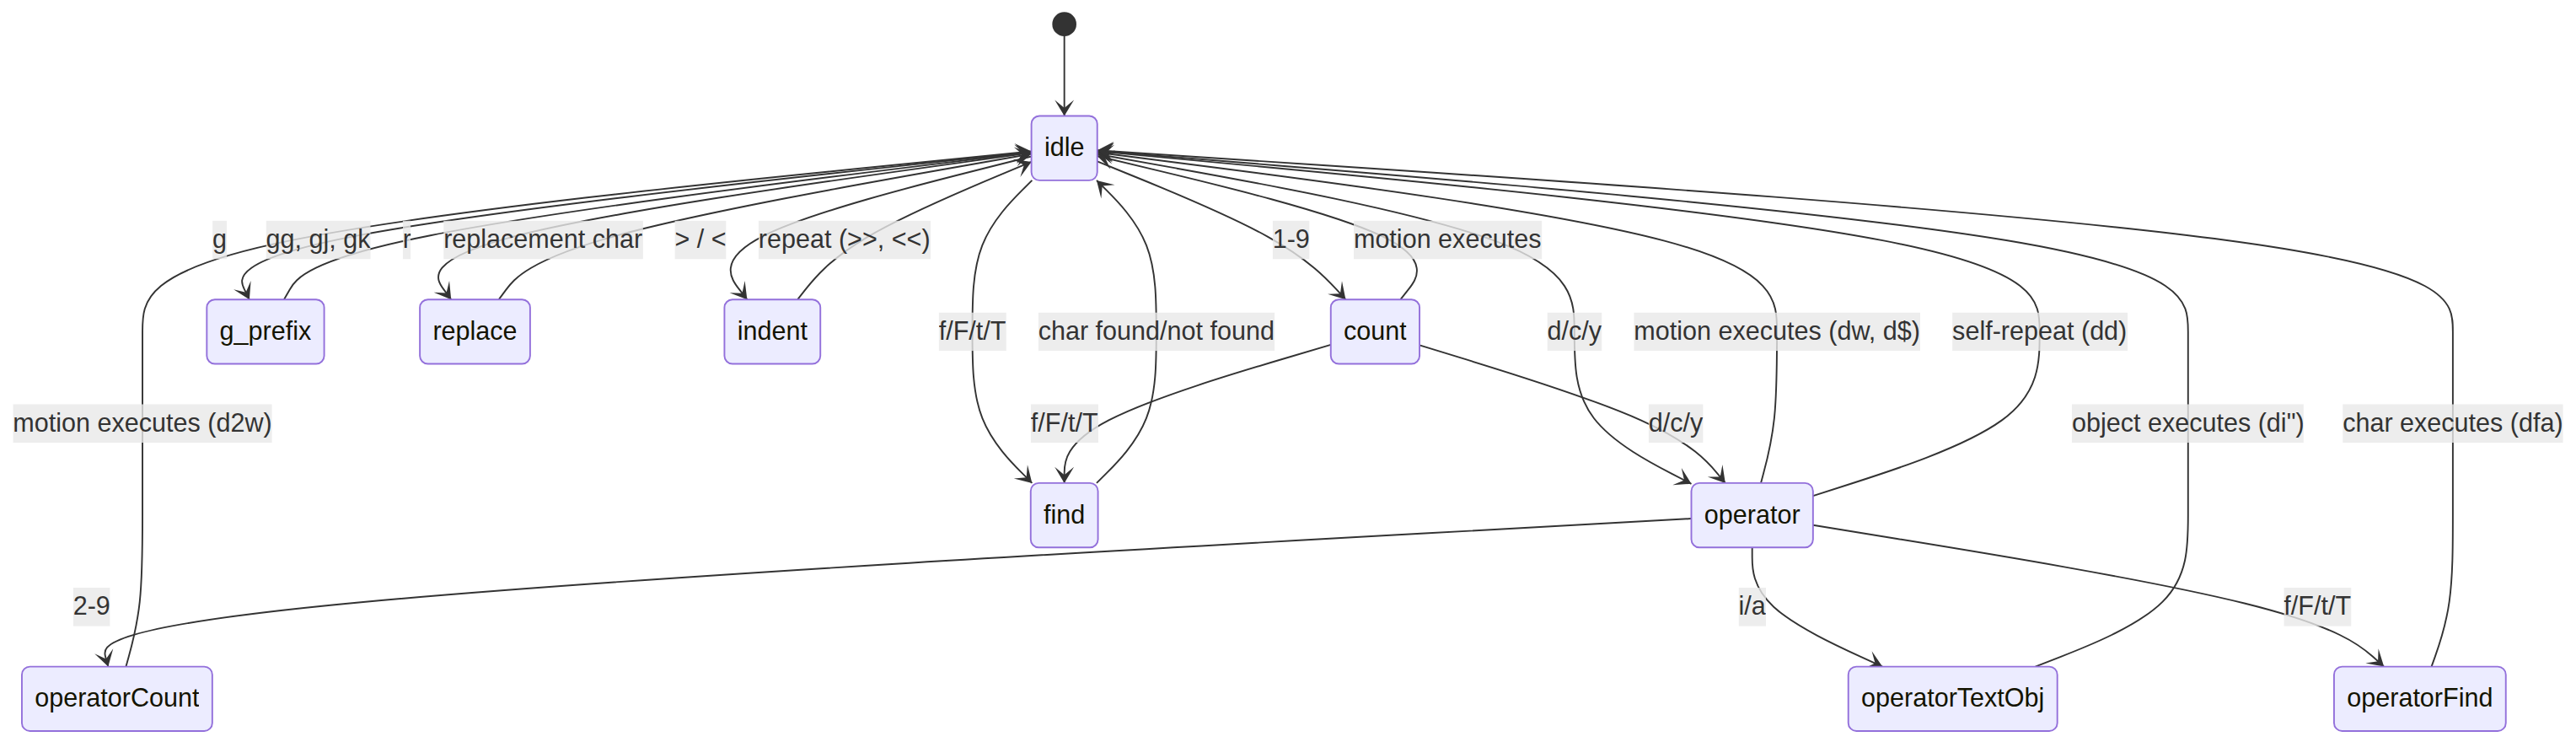
\includegraphics[width=16.67in,height=4.81in]{book/ch14-input-interaction_files/figure-latex/mermaid-figure-2.png}

From \texttt{idle}, pressing \texttt{d} enters the \texttt{operator}
state. From \texttt{operator}, pressing \texttt{w} executes
\texttt{delete} with the \texttt{w} motion. Pressing \texttt{d} again
(\texttt{dd}) triggers a line deletion. Pressing \texttt{2} enters
\texttt{operatorCount}, so \texttt{d2w} becomes ``delete the next 2
words.'' Pressing \texttt{i} enters \texttt{operatorTextObj}, so
\texttt{di"} becomes ``delete inside quotes.'' Every intermediate state
carries exactly the context needed for the next transition -- no more,
no less.

\subsection{Transitions as Pure
Functions}\label{transitions-as-pure-functions}

The \texttt{transition()} function dispatches on the current state type
to one of 10 handler functions. Each returns a
\texttt{TransitionResult}:

\begin{Shaded}
\begin{Highlighting}[]
\KeywordTok{type}\NormalTok{ TransitionResult }\OperatorTok{=}\NormalTok{ \{}
\NormalTok{  next}\OperatorTok{?:}\NormalTok{ CommandState}\OperatorTok{;}    \CommentTok{// New state (omitted = stay in current)}
\NormalTok{  execute}\OperatorTok{?:}\NormalTok{ () }\KeywordTok{=\textgreater{}} \DataTypeTok{void}\OperatorTok{;}   \CommentTok{// Side effect (omitted = no action yet)}
\NormalTok{\}}
\end{Highlighting}
\end{Shaded}

Side effects are returned, not executed. The transition function is pure
-- given a state and a key, it returns the next state and optionally a
closure that performs the action. The caller decides when to run the
effect. This makes the state machine trivially testable: feed it states
and keys, assert on the returned states, ignore the closures. It also
means the transition function has no dependencies on the editor state,
the cursor position, or the buffer content. Those details are captured
by the closure at creation time, not consumed by the state machine at
transition time.

The \texttt{fromIdle} handler is the entry point and covers the full vim
vocabulary:

\begin{itemize}
\tightlist
\item
  \textbf{Count prefix}: \texttt{1-9} enters the \texttt{count} state,
  accumulating digits. \texttt{0} is special -- it is the ``start of
  line'' motion, not a count digit, unless digits have already been
  accumulated
\item
  \textbf{Operators}: \texttt{d}, \texttt{c}, \texttt{y} enter the
  \texttt{operator} state, waiting for a motion or text object to define
  the range
\item
  \textbf{Find}: \texttt{f}, \texttt{F}, \texttt{t}, \texttt{T} enter
  the \texttt{find} state, waiting for a character to search for
\item
  \textbf{G-prefix}: \texttt{g} enters the \texttt{g} state for
  composite commands (\texttt{gg}, \texttt{gj}, \texttt{gk})
\item
  \textbf{Replace}: \texttt{r} enters the \texttt{replace} state,
  waiting for the replacement character
\item
  \textbf{Indent}: \texttt{\textgreater{}}, \texttt{\textless{}} enter
  the \texttt{indent} state (for \texttt{\textgreater{}\textgreater{}}
  and \texttt{\textless{}\textless{}})
\item
  \textbf{Simple motions}: \texttt{h/j/k/l/w/b/e/W/B/E/0/\^{}/\$}
  execute immediately, moving the cursor
\item
  \textbf{Immediate commands}: \texttt{x} (delete char),
  \texttt{\textasciitilde{}} (toggle case), \texttt{J} (join lines),
  \texttt{p/P} (paste), \texttt{D/C/Y} (operator shortcuts), \texttt{G}
  (go to end), \texttt{.} (dot-repeat), \texttt{;/,} (find repeat),
  \texttt{u} (undo), \texttt{i/I/a/A/o/O} (enter insert mode)
\end{itemize}

\subsection{Motions, Operators, and Text
Objects}\label{motions-operators-and-text-objects}

\textbf{Motions} are pure functions mapping a key to a cursor position.
\texttt{resolveMotion(key,\ cursor,\ count)} applies the motion
\texttt{count} times, short-circuiting if the cursor stops moving (you
cannot move left past column 0). This short-circuit is important for
\texttt{3w} at the end of a line -- it stops at the last word rather
than wrapping or erroring.

Motions are classified by how they interact with operators:

\begin{itemize}
\tightlist
\item
  \textbf{Exclusive} (default) -- the character at the destination is
  NOT included in the range. \texttt{dw} deletes up to but not including
  the first character of the next word
\item
  \textbf{Inclusive} (\texttt{e}, \texttt{E}, \texttt{\$}) -- the
  character at the destination IS included. \texttt{de} deletes through
  the last character of the current word
\item
  \textbf{Linewise} (\texttt{j}, \texttt{k}, \texttt{G}, \texttt{gg},
  \texttt{gj}, \texttt{gk}) -- when used with operators, the range
  extends to cover full lines. \texttt{dj} deletes the current line and
  the one below, not just the characters between the two cursor
  positions
\end{itemize}

\textbf{Operators} apply to a range. \texttt{delete} removes text and
saves it to the register. \texttt{change} removes text and enters insert
mode. \texttt{yank} copies to the register without modification. The
\texttt{cw}/\texttt{cW} special case follows vim convention: change-word
goes to the end of the current word, not the start of the next word
(unlike \texttt{dw}).

One interesting edge case: \texttt{{[}Image\ \#N{]}} chip snapping. When
a word motion lands inside an image reference chip (rendered as a single
visual unit in the terminal), the range extends to cover the entire
chip. This prevents partial deletions of what the user perceives as an
atomic element -- you cannot delete half of \texttt{{[}Image\ \#3{]}}
because the motion system treats the entire chip as a single word.

Additional commands cover the full expected vim vocabulary: \texttt{x}
(delete character), \texttt{r} (replace character),
\texttt{\textasciitilde{}} (toggle case), \texttt{J} (join lines),
\texttt{p}/\texttt{P} (paste with linewise/characterwise awareness),
\texttt{\textgreater{}\textgreater{}} / \texttt{\textless{}\textless{}}
(indent/outdent with 2-space stops), \texttt{o}/\texttt{O} (open line
below/above and enter insert mode).

\textbf{Text objects} find boundaries around the cursor. They answer the
question: ``what is the `thing' the cursor is inside?''

Word objects (\texttt{iw}, \texttt{aw}, \texttt{iW}, \texttt{aW})
segment text into graphemes, classify each as word-character,
whitespace, or punctuation, and expand the selection to the word
boundary. The \texttt{i} (inner) variant selects just the word. The
\texttt{a} (around) variant includes surrounding whitespace -- trailing
whitespace preferred, falling back to leading if at line end. The
uppercase variants (\texttt{W}, \texttt{aW}) treat any non-whitespace
sequence as a word, ignoring punctuation boundaries.

Quote objects (\texttt{i"}, \texttt{a"}, \texttt{i\textquotesingle{}},
\texttt{a\textquotesingle{}}, \texttt{i\textasciigrave{}},
\texttt{a\textasciigrave{}}) find paired quotes on the current line.
Pairs are matched in order (first and second quote form a pair, third
and fourth form the next pair, etc.). If the cursor is between the first
and second quote, that is the match. The \texttt{a} variant includes the
quote characters; the \texttt{i} variant excludes them.

Bracket objects (\texttt{ib}/\texttt{i(}, \texttt{ab}/\texttt{a(},
\texttt{i{[}}/\texttt{a{[}},
\texttt{iB}/\texttt{i\{}/\texttt{aB}/\texttt{a\{},
\texttt{i\textless{}}/\texttt{a\textless{}}) do depth-tracking search
for matching delimiters. They search outward from the cursor,
maintaining a nesting count, until they find the matching pair at depth
zero. This correctly handles nested brackets -- \texttt{d\ i\ (} inside
\texttt{foo((bar))} deletes \texttt{bar}, not \texttt{(bar)}.

\subsection{Persistent State and
Dot-Repeat}\label{persistent-state-and-dot-repeat}

The vim mode maintains a \texttt{PersistentState} that survives across
commands -- the ``memory'' that makes vim feel like vim:

\begin{Shaded}
\begin{Highlighting}[]
\KeywordTok{interface}\NormalTok{ PersistentState \{}
\NormalTok{  lastChange}\OperatorTok{:}\NormalTok{ RecordedChange}\OperatorTok{;}   \CommentTok{// For dot{-}repeat}
\NormalTok{  lastFind}\OperatorTok{:}\NormalTok{ \{ type}\OperatorTok{:}\NormalTok{ FindType}\OperatorTok{;}\NormalTok{ char}\OperatorTok{:} \DataTypeTok{string}\NormalTok{ \}}\OperatorTok{;}  \CommentTok{// For ; and ,}
\NormalTok{  register}\OperatorTok{:} \DataTypeTok{string}\OperatorTok{;}             \CommentTok{// Yank buffer}
\NormalTok{  registerIsLinewise}\OperatorTok{:} \DataTypeTok{boolean}\OperatorTok{;}  \CommentTok{// Paste behavior flag}
\NormalTok{\}}
\end{Highlighting}
\end{Shaded}

Every mutating command records itself as a \texttt{RecordedChange} -- a
discriminated union covering insert, operator+motion, operator+textObj,
operator+find, replace, delete-char, toggle-case, indent, open-line, and
join. The \texttt{.} command replays \texttt{lastChange} from persistent
state, using the recorded count, operator, and motion to reproduce the
exact same edit at the current cursor position.

Find-repeat (\texttt{;} and \texttt{,}) uses \texttt{lastFind}. The
\texttt{;} command repeats the last find in the same direction. The
\texttt{,} command flips the direction: \texttt{f} becomes \texttt{F},
\texttt{t} becomes \texttt{T}, and vice versa. This means after
\texttt{fa} (find next `a'), \texttt{;} finds the next `a' forward and
\texttt{,} finds the next `a' backward -- without the user having to
remember which direction they were searching.

The register tracks yanked and deleted text. When register content ends
with \texttt{\textbackslash{}n}, it is flagged as linewise, which
changes paste behavior: \texttt{p} inserts below the current line (not
after the cursor), and \texttt{P} inserts above. This distinction is
invisible to the user but critical for the ``delete a line, paste it
somewhere else'' workflow that vim users rely on constantly.

\begin{center}\rule{0.5\linewidth}{0.5pt}\end{center}

\section{Virtual Scrolling}\label{virtual-scrolling}

Long Claude Code sessions produce long conversations. A heavy debugging
session might generate 200+ messages, each containing markdown, code
blocks, tool use results, and permission records. Without
virtualization, React would maintain 200+ component subtrees in memory,
each with its own state, effects, and memoization caches. The DOM tree
would contain thousands of nodes. Yoga layout would visit all of them on
every frame. The terminal would be unusable.

The \texttt{VirtualMessageList} component solves this by rendering only
the messages visible in the viewport plus a small buffer above and
below. In a conversation with hundreds of messages, this is the
difference between mounting 500 React subtrees (each with markdown
parsing, syntax highlighting, and tool use blocks) and mounting 15.

The component maintains:

\begin{itemize}
\tightlist
\item
  \textbf{Height cache} per message, invalidated when terminal column
  count changes
\item
  \textbf{Jump handle} for transcript search navigation (jump to index,
  next/previous match)
\item
  \textbf{Search text extraction} with warm-cache support (pre-lowercase
  all messages when the user enters \texttt{/})
\item
  \textbf{Sticky prompt tracking} -- when the user scrolls away from the
  input, their last prompt text appears at the top as context
\item
  \textbf{Message actions navigation} -- cursor-based message selection
  for the rewind feature
\end{itemize}

The \texttt{useVirtualScroll} hook computes which messages to mount
based on \texttt{scrollTop}, \texttt{viewportHeight}, and cumulative
message heights. It maintains scroll clamp bounds on the
\texttt{ScrollBox} to prevent blank screens when burst \texttt{scrollTo}
calls race past React's async re-render -- a classic problem with
virtualized lists where the scroll position can outrun the DOM update.

The interaction between virtual scrolling and the markdown token cache
is worth noting. When a message scrolls out of the viewport, its React
subtree unmounts. When the user scrolls back, the subtree remounts.
Without caching, this would mean re-parsing the markdown for every
message the user scrolls past. The module-level LRU cache (500 entries,
keyed by content hash) ensures that the expensive
\texttt{marked.lexer()} call happens at most once per unique message
content, regardless of how many times the component mounts and unmounts.

The \texttt{ScrollBox} component itself provides an imperative API via
\texttt{useImperativeHandle}:

\begin{itemize}
\tightlist
\item
  \texttt{scrollTo(y)} -- absolute scroll, breaks sticky-scroll mode
\item
  \texttt{scrollBy(dy)} -- accumulates into \texttt{pendingScrollDelta},
  drained by the renderer at a capped rate
\item
  \texttt{scrollToElement(el,\ offset)} -- defers position read to
  render time via \texttt{scrollAnchor}
\item
  \texttt{scrollToBottom()} -- re-enables sticky-scroll mode
\item
  \texttt{setClampBounds(min,\ max)} -- constrains the virtual scroll
  window
\end{itemize}

All scroll mutations go directly to DOM node properties and schedule
renders via microtask, bypassing React's reconciler. The
\texttt{markScrollActivity()} call signals background intervals
(spinners, timers) to skip their next tick, reducing event-loop
contention during active scrolling. This is a cooperative scheduling
pattern: the scroll path tells background work ``I am in a
latency-sensitive operation, please yield.'' Background intervals check
this flag before scheduling their next tick and delay by one frame if
scrolling is active. The result is consistently smooth scrolling even
when multiple spinners and timers are running in the background.

\begin{center}\rule{0.5\linewidth}{0.5pt}\end{center}

\section{Apply This: Building a Context-Aware Keybinding
System}\label{apply-this-building-a-context-aware-keybinding-system}

Claude Code's keybinding architecture offers a template for any
application with modal input -- editors, IDEs, drawing tools, terminal
multiplexers. The key insights:

\textbf{Separate bindings from handlers.} Bindings are data (which key
maps to which action name). Handlers are code (what happens when the
action fires). Keeping them separate means bindings can be serialized to
JSON for user customization, while handlers remain in the components
that own the relevant state. A user can rebind \texttt{ctrl+k} to
\texttt{chat:submit} without touching any component code.

\textbf{Context as a first-class concept.} Instead of one flat keymap,
define contexts that activate and deactivate based on application state.
When a dialog opens, the \texttt{Confirmation} context activates and its
bindings take precedence over \texttt{Chat} bindings. When the dialog
closes, \texttt{Chat} bindings resume. This eliminates the conditional
soup of
\texttt{if\ (dialogOpen\ \&\&\ key\ ===\ \textquotesingle{}y\textquotesingle{})}
scattered through event handlers.

\textbf{Chord state as an explicit machine.} Multi-key sequences
(chords) are not a special case of single-key bindings -- they are a
different kind of binding that requires a state machine with timeout and
cancellation semantics. Making this explicit (with a dedicated
\texttt{ChordInterceptor} component and a \texttt{pendingChordRef})
prevents subtle bugs where the second keystroke of a chord is consumed
by a different handler because React's state update had not yet
propagated.

\textbf{Reserve early, warn clearly.} Identify keys that cannot be
rebound (system shortcuts, terminal control characters) at definition
time, not at resolution time. When a user tries to bind \texttt{ctrl+c},
show an error during configuration loading rather than silently
accepting a binding that will never fire. This is the difference between
a keybinding system that works and one that produces mysterious bug
reports.

\textbf{Design for terminal diversity.} Claude Code's keybinding system
defines platform-specific alternatives at the binding level, not the
handler level. Image paste is \texttt{ctrl+v} or \texttt{alt+v}
depending on the OS. Mode cycling is \texttt{shift+tab} or
\texttt{meta+m} depending on VT mode support. The handler for each
action is the same regardless of which key triggers it. This means
testing covers one code path per action, not one per platform-key
combination. And when a new terminal quirk surfaces (Windows Terminal
lacking VT mode before Node 24.2.0, for example), the fix is a single
conditional in the binding definition, not a scattered set of
\texttt{if\ (platform\ ===\ \textquotesingle{}windows\textquotesingle{})}
checks in handler code.

\textbf{Provide escape hatches.} The null-action unbinding mechanism is
small but important. A user who runs Claude Code inside a terminal
multiplexer might find that \texttt{ctrl+t} (toggle todos) conflicts
with their multiplexer's tab-switching shortcut. By adding
\texttt{\{\ "ctrl+t":\ null\ \}} to their keybindings.json, they disable
the binding entirely. The key press passes through to the multiplexer.
Without null unbinding, the user's only option would be to rebind
\texttt{ctrl+t} to some other action they do not want, or to reconfigure
their multiplexer -- neither of which is a good experience.

The vim mode implementation adds one more lesson: \textbf{make the type
system enforce your state machine}. The 12-variant \texttt{CommandState}
union makes it impossible to forget a state in a switch statement. The
\texttt{TransitionResult} type separates state changes from side
effects, making the machine testable as a pure function. If your
application has modal input, express the modes as a discriminated union
and let the compiler verify exhaustiveness. The time spent defining the
types pays for itself in eliminated runtime bugs.

Consider the alternative: a vim implementation using mutable state and
imperative conditionals. The \texttt{fromOperator} handler would be a
nest of
\texttt{if\ (mode\ ===\ \textquotesingle{}operator\textquotesingle{}\ \&\&\ pendingCount\ !==\ null\ \&\&\ isDigit(key))}
checks, with each branch mutating shared variables. Adding a new state
(say, a macro-recording mode) would require auditing every branch to
ensure the new state is handled. With a discriminated union, the
compiler does the audit -- the PR that adds the new variant will not
build until every switch statement handles it.

This is the deeper lesson of Claude Code's input system: at every layer
-- tokenizer, parser, keybinding resolver, vim state machine -- the
architecture converts unstructured input into typed, exhaustively
handled structures as early as possible. Raw bytes become
\texttt{ParsedKey} at the parser boundary. \texttt{ParsedKey} becomes an
action name at the keybinding boundary. The action name becomes a typed
handler at the component boundary. Each conversion narrows the space of
possible states, and each narrowing is enforced by TypeScript's type
system. By the time a keystroke reaches application logic, the ambiguity
is gone. There is no ``what if the key is undefined?'' There is no
``what if the modifier combination is impossible?'' The types have
already forbidden those states from existing.

The two chapters together tell one story. Chapter 13 showed how the
rendering system eliminates unnecessary work -- blitting unchanged
regions, interning repeated values, diffing at the cell level, tracking
damage bounds. Chapter 14 showed how the input system eliminates
ambiguity -- parsing five protocols into one type, resolving keys
against contextual bindings, expressing modal state as exhaustive
unions. The rendering system answers ``how do you paint 24,000 cells 60
times per second?'' The input system answers ``how do you turn a byte
stream into meaningful actions across a fragmented ecosystem?'' Both
answers follow the same principle: push complexity to the boundaries,
where it can be handled once and correctly, so that everything
downstream operates on clean, typed, well-bounded data. The terminal is
chaos. The application is order. The boundary code does the hard work of
converting one into the other.

\begin{center}\rule{0.5\linewidth}{0.5pt}\end{center}

\section{Summary: Two Systems, One Design
Philosophy}\label{summary-two-systems-one-design-philosophy}

Chapters 13 and 14 covered the two halves of the terminal interface:
output and input. Despite their different concerns, both systems follow
the same architectural principles.

\textbf{Interning and indirection.} The rendering system interns
characters, styles, and hyperlinks into pools, replacing string
comparisons with integer comparisons throughout the hot path. The input
system interns escape sequences into structured \texttt{ParsedKey}
objects at the parser boundary, replacing byte-level pattern matching
with typed field access throughout the handler path.

\textbf{Layered elimination of work.} The rendering system stacks five
optimizations (dirty flags, blit, damage rectangles, cell-level diff,
patch optimization) that each eliminate a category of unnecessary
computation. The input system stacks three (tokenizer, protocol parser,
keybinding resolver) that each eliminate a category of ambiguity.

\textbf{Pure functions and typed state machines.} The vim mode is a pure
state machine with typed transitions. The keybinding resolver is a pure
function from (key, contexts, chord-state) to resolution-result. The
rendering pipeline is a pure function from (DOM tree, previous screen)
to (new screen, patches). Side effects happen at the boundaries --
writing to stdout, dispatching to React -- not in the core logic.

\textbf{Graceful degradation across environments.} The rendering system
adapts to terminal size, alt-screen support, and synchronized-update
protocol availability. The input system adapts to Kitty keyboard
protocol, xterm modifyOtherKeys, legacy VT sequences, and multiplexer
passthrough requirements. Neither system requires a specific terminal to
function; both get better on more capable terminals.

These principles are not specific to terminal applications. They apply
to any system that must process high-frequency input and produce
low-latency output across a diverse set of runtime environments. The
terminal just happens to be an environment where the constraints are
sharp enough that violating these principles produces immediately
visible degradation -- a dropped frame, a swallowed keystroke, a
flicker. That sharpness makes it an excellent teacher.

The next chapter moves from the UI layer to the protocol layer: how
Claude Code implements MCP -- the universal tool protocol that lets any
external service become a first-class tool. The terminal UI handles the
last mile of the user experience -- converting data structures into
pixels on a screen and keystrokes into application actions. MCP handles
the first mile of extensibility -- discovering, connecting, and
executing tools that live outside the agent's own codebase. Between
them, the memory system (Chapter 11) and the skills/hooks system
(Chapter 12) define the intelligence and control layers. The quality
ceiling of the entire system depends on all four: no amount of model
intelligence compensates for a laggy UI, and no amount of rendering
performance compensates for a model that cannot reach the tools it
needs.

\part{Part VI: Connectivity}

\chapter{Chapter 15: MCP -- The Universal Tool
Protocol}\label{chapter-15-mcp-the-universal-tool-protocol}

\section{Why MCP Matters Beyond Claude
Code}\label{why-mcp-matters-beyond-claude-code}

Every other chapter in this book is about Claude Code's internals. This
one is different. The Model Context Protocol is an open specification
that any agent can implement, and Claude Code's MCP subsystem is one of
the most complete production clients in existence. If you are building
an agent that needs to call external tools -- any agent, in any
language, on any model -- the patterns in this chapter transfer
directly.

The core proposition is straightforward: MCP defines a JSON-RPC 2.0
protocol for tool discovery and invocation between a client (the agent)
and a server (the tool provider). The client sends \texttt{tools/list}
to discover what a server offers, then \texttt{tools/call} to execute.
The server describes each tool with a name, description, and JSON Schema
for its inputs. That is the entire contract. Everything else --
transport selection, authentication, config loading, tool name
normalization -- is the implementation work that turns a clean spec into
something that survives contact with the real world.

Claude Code's MCP implementation spans four core files:
\texttt{types.ts}, \texttt{client.ts}, \texttt{auth.ts}, and
\texttt{InProcessTransport.ts}. Together they support eight transport
types, seven configuration scopes, OAuth discovery across two RFCs, and
a tool wrapping layer that makes MCP tools indistinguishable from
built-in ones -- the same \texttt{Tool} interface covered in Chapter 6.
This chapter walks through each layer.

\begin{center}\rule{0.5\linewidth}{0.5pt}\end{center}

\section{Eight Transport Types}\label{eight-transport-types}

The first design decision in any MCP integration is how the client talks
to the server. Claude Code supports eight transport configurations:

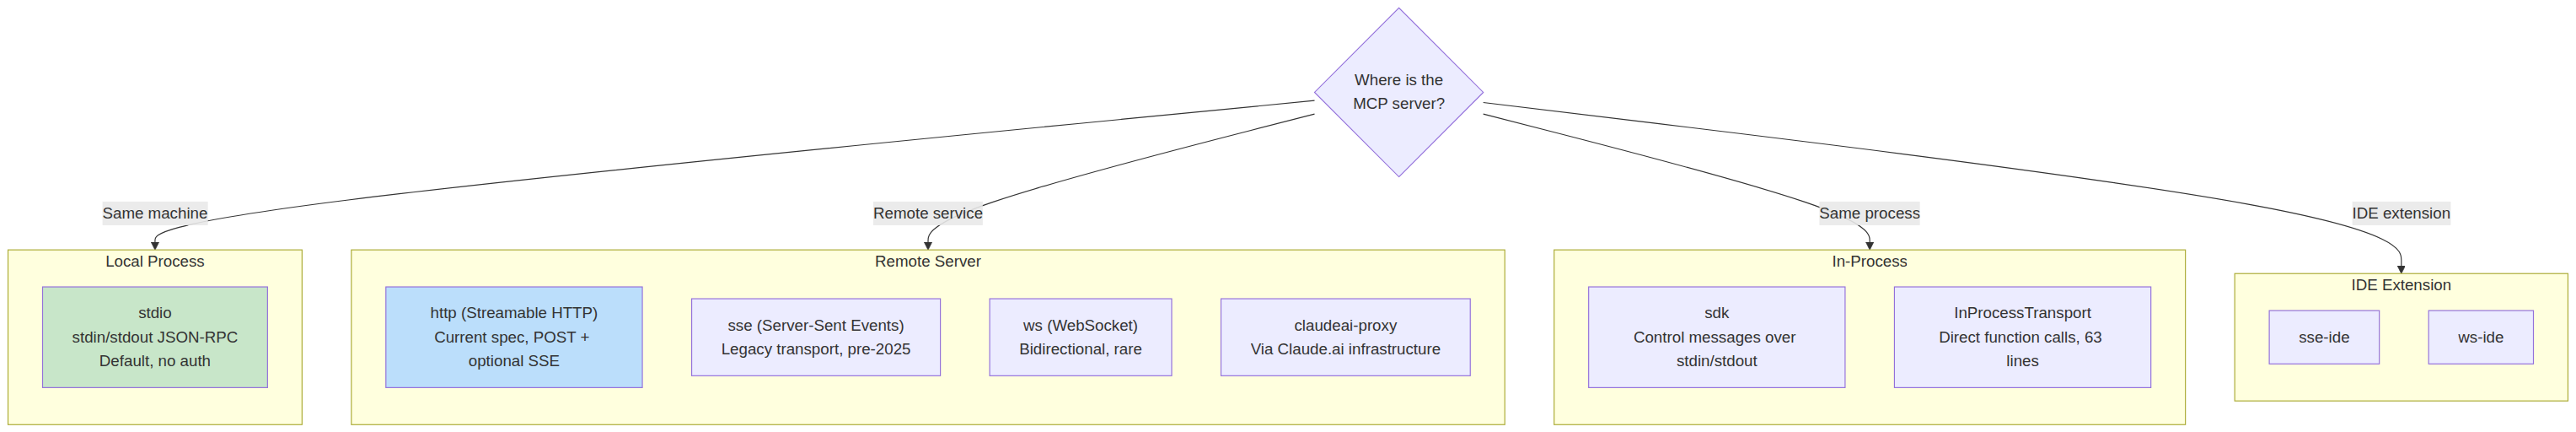
\includegraphics[width=27.2in,height=4.56in]{book/ch15-mcp_files/figure-latex/mermaid-figure-1.png}

Three design choices are worth noting. First, \texttt{stdio} is the
default -- when \texttt{type} is omitted, the system assumes a local
subprocess. This is backwards-compatible with the earliest MCP configs.
Second, the fetch wrappers stack: timeout wrapping outside step-up
detection, outside the base fetch. Each wrapper handles one concern.
Third, the \texttt{ws-ide} branch has a Bun/Node runtime split -- Bun's
\texttt{WebSocket} accepts proxy and TLS options natively, while Node
requires the \texttt{ws} package.

\textbf{When to use which.} For local tools (filesystem, database,
custom scripts), \texttt{stdio} -- no network, no auth, just pipes. For
remote services, \texttt{http} (Streamable HTTP) is the current spec
recommendation. \texttt{sse} is legacy but widely deployed. The
\texttt{sdk}, IDE, and \texttt{claudeai-proxy} types are internal to
their respective ecosystems.

\begin{center}\rule{0.5\linewidth}{0.5pt}\end{center}

\section{Configuration Loading and
Scoping}\label{configuration-loading-and-scoping}

MCP server configs load from seven scopes, merged and deduplicated:

\begin{longtable}[]{@{}lll@{}}
\toprule\noalign{}
Scope & Source & Trust \\
\midrule\noalign{}
\endhead
\bottomrule\noalign{}
\endlastfoot
\texttt{local} & \texttt{.mcp.json} in working directory & Requires user
approval \\
\texttt{user} & \texttt{\textasciitilde{}/.claude.json} mcpServers field
& User-managed \\
\texttt{project} & Project-level config & Shared project settings \\
\texttt{enterprise} & Managed enterprise config & Pre-approved by org \\
\texttt{managed} & Plugin-provided servers & Auto-discovered \\
\texttt{claudeai} & Claude.ai web interface & Pre-authorized via web \\
\texttt{dynamic} & Runtime injection (SDK) & Programmatically added \\
\end{longtable}

\textbf{Deduplication is content-based, not name-based.} Two servers
with different names but the same command or URL are recognized as the
same server. The \texttt{getMcpServerSignature()} function computes a
canonical key: \texttt{stdio:{[}"command","arg1"{]}} for local servers,
\texttt{url:https://example.com/mcp} for remote ones. Plugin-provided
servers whose signature matches a manual config are suppressed.

\begin{center}\rule{0.5\linewidth}{0.5pt}\end{center}

\section{Tool Wrapping: From MCP to Claude
Code}\label{tool-wrapping-from-mcp-to-claude-code}

When a connection succeeds, the client calls \texttt{tools/list}. Each
tool definition is transformed into Claude Code's internal \texttt{Tool}
interface -- the same interface used by built-in tools. After wrapping,
the model cannot distinguish between a built-in tool and an MCP tool.

The wrapping process has four stages:

\textbf{1. Name normalization.} \texttt{normalizeNameForMCP()} replaces
invalid characters with underscores. The fully qualified name follows
\texttt{mcp\_\_\{serverName\}\_\_\{toolName\}}.

\textbf{2. Description truncation.} Capped at 2,048 characters.
OpenAPI-generated servers have been observed dumping 15-60KB into
\texttt{tool.description} -- roughly 15,000 tokens per turn for a single
tool.

\textbf{3. Schema passthrough.} The tool's \texttt{inputSchema} passes
directly to the API. No transformation, no validation at wrapping time.
Schema errors surface at call time, not registration time.

\textbf{4. Annotation mapping.} MCP annotations map to behavior flags:
\texttt{readOnlyHint} marks tools safe for concurrent execution (as
discussed in Chapter 7's streaming executor), \texttt{destructiveHint}
triggers extra permission scrutiny. These annotations come from the MCP
server -- a malicious server could mark a destructive tool as read-only.
This is an accepted trust boundary, but one worth understanding: the
user opted into the server, and a malicious server marking destructive
tools as read-only is a real attack vector. The system accepts this
tradeoff because the alternative -- ignoring annotations entirely --
would prevent legitimate servers from improving the user experience.

\begin{center}\rule{0.5\linewidth}{0.5pt}\end{center}

\section{OAuth for MCP Servers}\label{oauth-for-mcp-servers}

Remote MCP servers often require authentication. Claude Code implements
the full OAuth 2.0 + PKCE flow with RFC-based discovery, Cross-App
Access, and error body normalization.

\subsection{Discovery Chain}\label{discovery-chain}

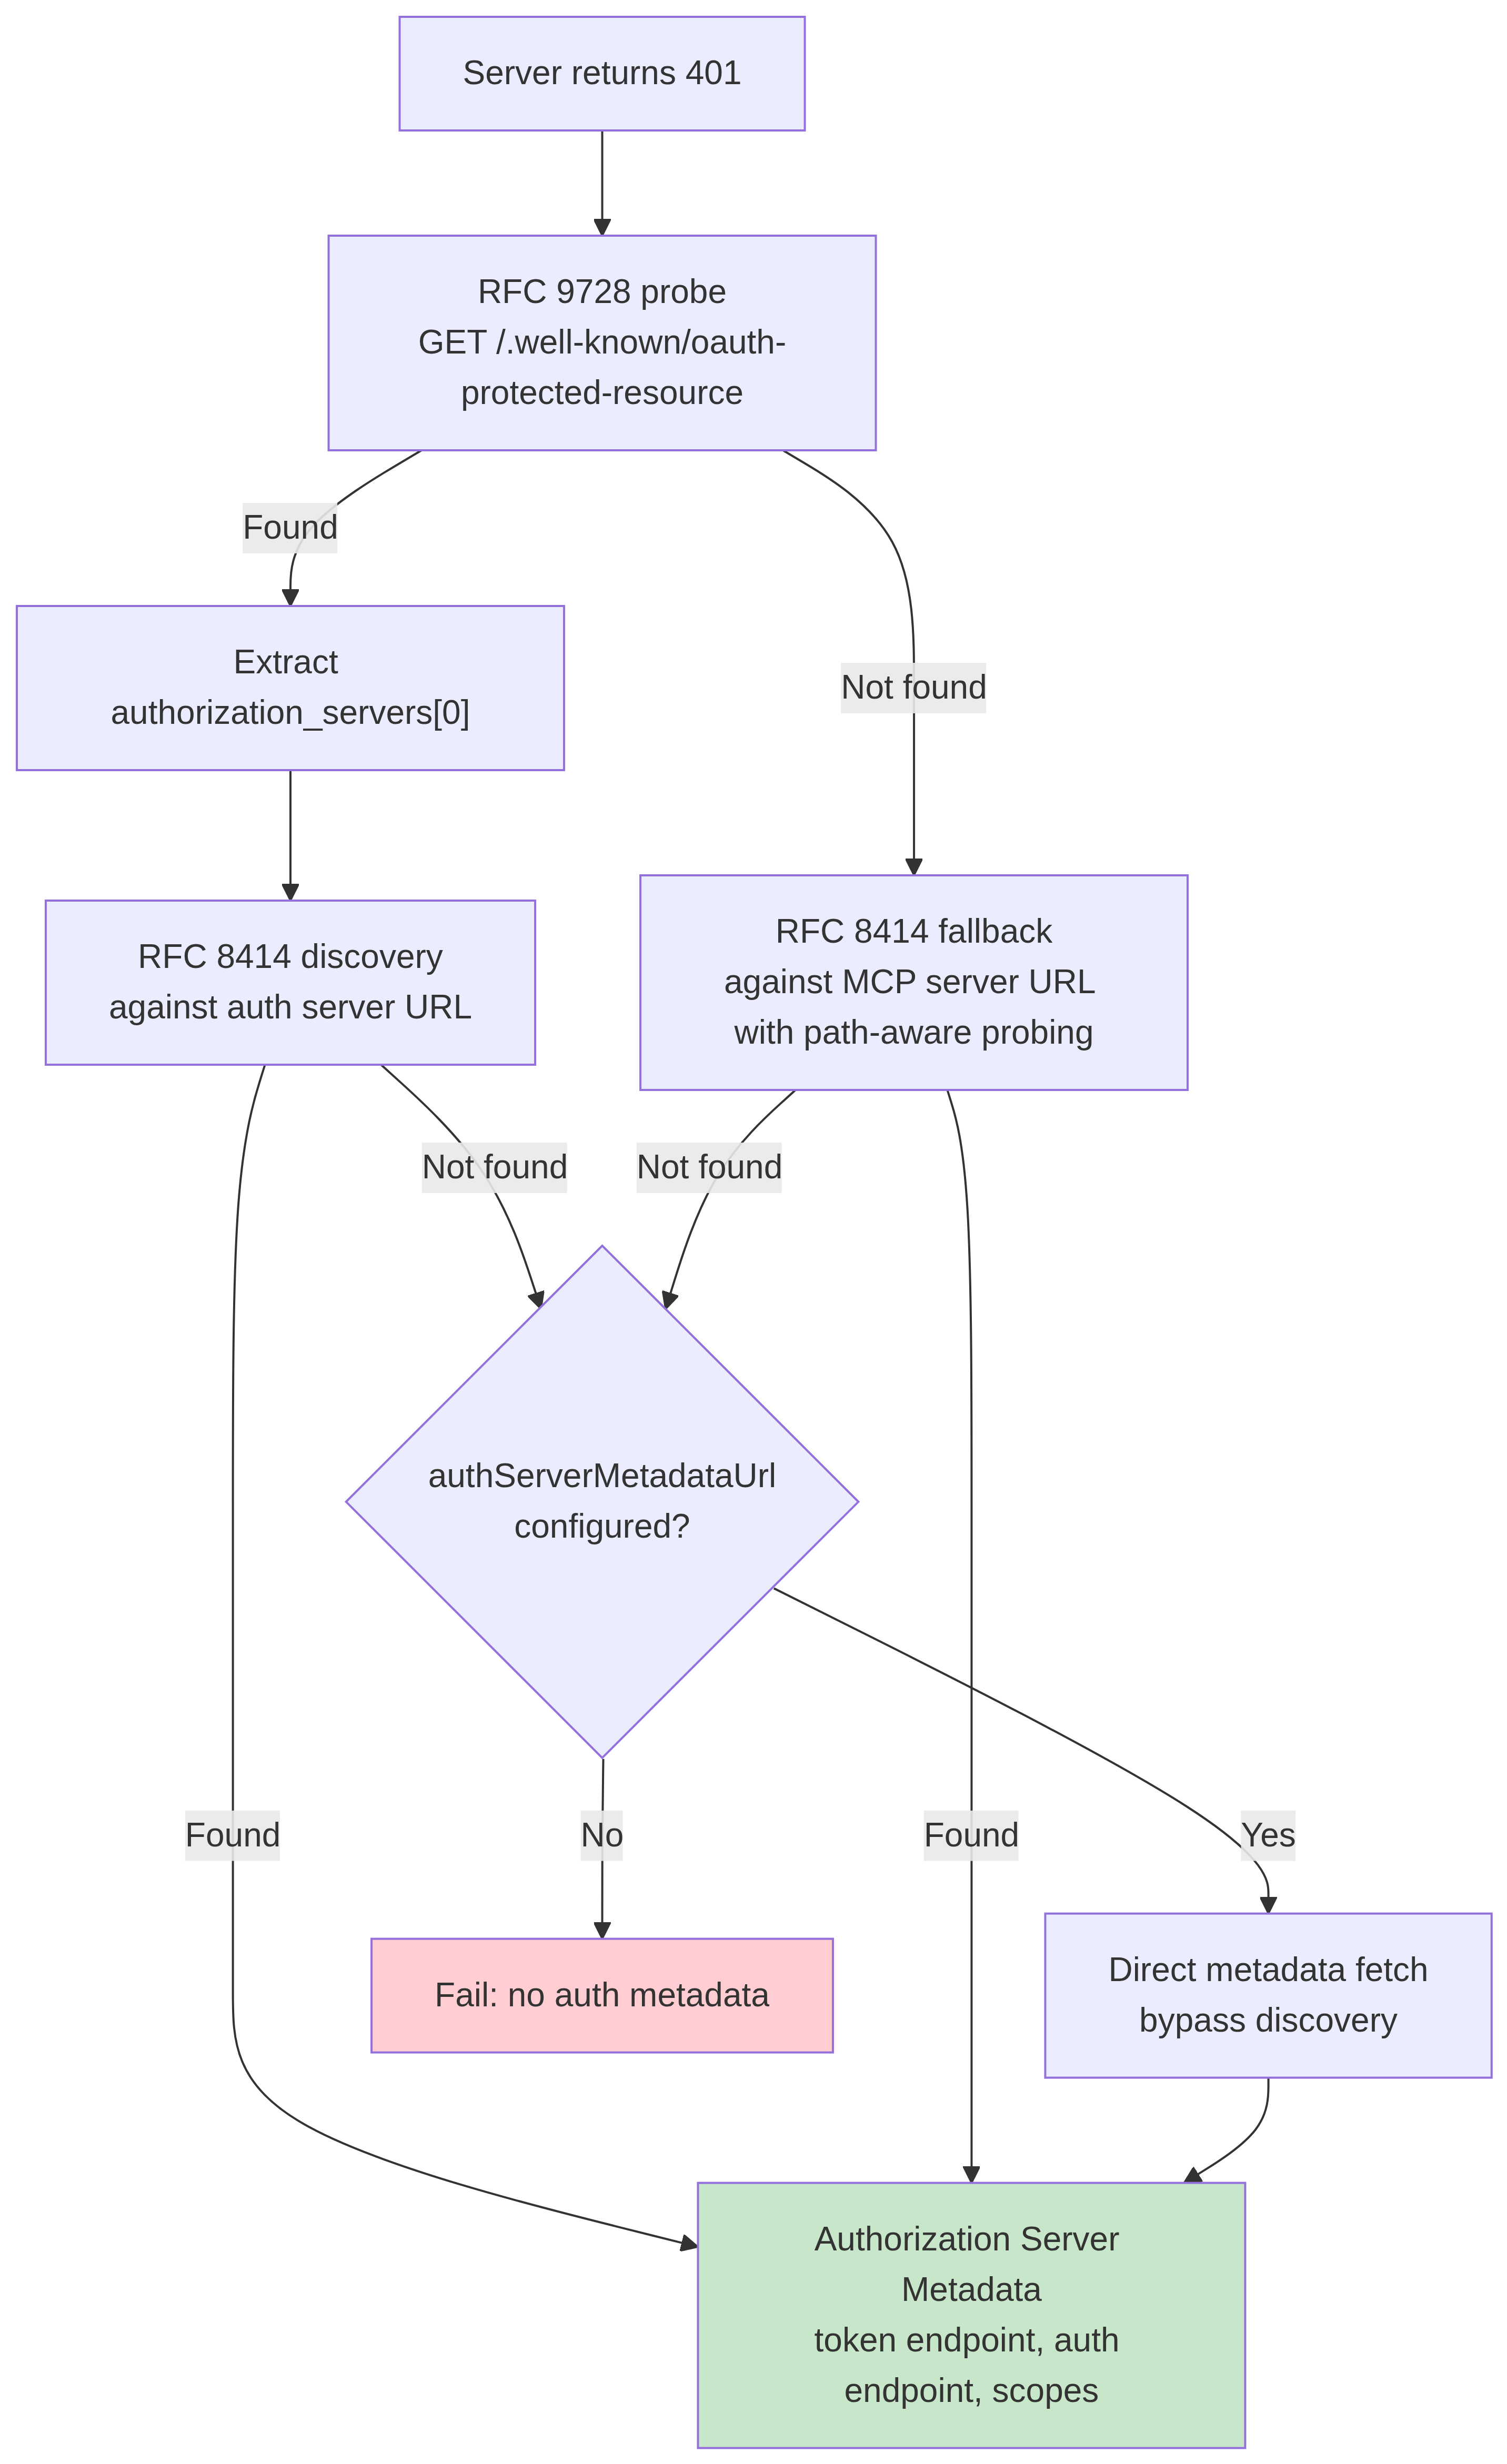
\includegraphics[width=7.47in,height=12.2in]{book/ch15-mcp_files/figure-latex/mermaid-figure-2.png}

The \texttt{authServerMetadataUrl} escape hatch exists because some
OAuth servers implement neither RFC.

\subsection{Cross-App Access (XAA)}\label{cross-app-access-xaa}

When an MCP server config has \texttt{oauth.xaa:\ true}, the system
performs federated token exchange through an Identity Provider -- one
IdP login unlocks multiple MCP servers.

\subsection{Error Body Normalization}\label{error-body-normalization}

The \texttt{normalizeOAuthErrorBody()} function handles OAuth servers
that violate the spec. Slack returns HTTP 200 for error responses with
the error buried in the JSON body. The function peeks at 2xx POST
response bodies, and when the body matches
\texttt{OAuthErrorResponseSchema} but not \texttt{OAuthTokensSchema},
rewrites the response to HTTP 400. It also normalizes Slack-specific
error codes (\texttt{invalid\_refresh\_token},
\texttt{expired\_refresh\_token}, \texttt{token\_expired}) to the
standard \texttt{invalid\_grant}.

\begin{center}\rule{0.5\linewidth}{0.5pt}\end{center}

\section{In-Process Transport}\label{in-process-transport}

Not every MCP server needs to be a separate process. The
\texttt{InProcessTransport} class enables running an MCP server and
client in the same process:

\begin{Shaded}
\begin{Highlighting}[]
\KeywordTok{class}\NormalTok{ InProcessTransport }\KeywordTok{implements}\NormalTok{ Transport \{}
  \KeywordTok{async} \FunctionTok{send}\NormalTok{(message}\OperatorTok{:}\NormalTok{ JSONRPCMessage)}\OperatorTok{:} \BuiltInTok{Promise}\OperatorTok{\textless{}}\DataTypeTok{void}\OperatorTok{\textgreater{}}\NormalTok{ \{}
    \ControlFlowTok{if}\NormalTok{ (}\KeywordTok{this}\OperatorTok{.}\AttributeTok{closed}\NormalTok{) }\ControlFlowTok{throw} \KeywordTok{new} \BuiltInTok{Error}\NormalTok{(}\StringTok{\textquotesingle{}Transport is closed\textquotesingle{}}\NormalTok{)}
    \FunctionTok{queueMicrotask}\NormalTok{(() }\KeywordTok{=\textgreater{}}\NormalTok{ \{ }\KeywordTok{this}\OperatorTok{.}\AttributeTok{peer}\OperatorTok{?.}\AttributeTok{onmessage}\OperatorTok{?.}\NormalTok{(message) \})}
\NormalTok{  \}}
  \KeywordTok{async} \FunctionTok{close}\NormalTok{()}\OperatorTok{:} \BuiltInTok{Promise}\OperatorTok{\textless{}}\DataTypeTok{void}\OperatorTok{\textgreater{}}\NormalTok{ \{}
    \ControlFlowTok{if}\NormalTok{ (}\KeywordTok{this}\OperatorTok{.}\AttributeTok{closed}\NormalTok{) }\ControlFlowTok{return}
    \KeywordTok{this}\OperatorTok{.}\AttributeTok{closed} \OperatorTok{=} \KeywordTok{true}
    \KeywordTok{this}\OperatorTok{.}\AttributeTok{onclose}\OperatorTok{?.}\NormalTok{()}
    \ControlFlowTok{if}\NormalTok{ (}\KeywordTok{this}\OperatorTok{.}\AttributeTok{peer} \OperatorTok{\&\&} \OperatorTok{!}\KeywordTok{this}\OperatorTok{.}\AttributeTok{peer}\OperatorTok{.}\AttributeTok{closed}\NormalTok{) \{}
      \KeywordTok{this}\OperatorTok{.}\AttributeTok{peer}\OperatorTok{.}\AttributeTok{closed} \OperatorTok{=} \KeywordTok{true}
      \KeywordTok{this}\OperatorTok{.}\AttributeTok{peer}\OperatorTok{.}\AttributeTok{onclose}\OperatorTok{?.}\NormalTok{()}
\NormalTok{    \}}
\NormalTok{  \}}
\NormalTok{\}}
\end{Highlighting}
\end{Shaded}

The entire file is 63 lines. Two design decisions deserve attention.
First, \texttt{send()} delivers via \texttt{queueMicrotask()} to prevent
stack depth issues in synchronous request/response cycles. Second,
\texttt{close()} cascades to the peer, preventing half-open states. The
Chrome MCP server and Computer Use MCP server both use this pattern.

\begin{center}\rule{0.5\linewidth}{0.5pt}\end{center}

\section{Connection Management}\label{connection-management}

\subsection{Connection States}\label{connection-states}

Each MCP server connection exists in one of five states:
\texttt{connected}, \texttt{failed}, \texttt{needs-auth} (with a
15-minute TTL cache to prevent 30 servers from independently discovering
the same expired token), \texttt{pending}, or \texttt{disabled}.

\subsection{Session Expiry Detection}\label{session-expiry-detection}

MCP's Streamable HTTP transport uses session IDs. When a server
restarts, requests return HTTP 404 with JSON-RPC error code -32001. The
\texttt{isMcpSessionExpiredError()} function checks both signals -- note
that it uses string inclusion on the error message to detect the error
code, which is pragmatic but fragile:

\begin{Shaded}
\begin{Highlighting}[]
\ImportTok{export} \KeywordTok{function} \FunctionTok{isMcpSessionExpiredError}\NormalTok{(error}\OperatorTok{:} \BuiltInTok{Error}\NormalTok{)}\OperatorTok{:} \DataTypeTok{boolean}\NormalTok{ \{}
  \KeywordTok{const}\NormalTok{ httpStatus }\OperatorTok{=} \StringTok{\textquotesingle{}code\textquotesingle{}} \KeywordTok{in}\NormalTok{ error }\OperatorTok{?}\NormalTok{ (error }\ImportTok{as} \DataTypeTok{any}\NormalTok{)}\OperatorTok{.}\AttributeTok{code} \OperatorTok{:} \KeywordTok{undefined}
  \ControlFlowTok{if}\NormalTok{ (httpStatus }\OperatorTok{!==} \DecValTok{404}\NormalTok{) }\ControlFlowTok{return} \KeywordTok{false}
  \ControlFlowTok{return}\NormalTok{ error}\OperatorTok{.}\AttributeTok{message}\OperatorTok{.}\FunctionTok{includes}\NormalTok{(}\StringTok{\textquotesingle{}"code":{-}32001\textquotesingle{}}\NormalTok{) }\OperatorTok{||}
\NormalTok{    error}\OperatorTok{.}\AttributeTok{message}\OperatorTok{.}\FunctionTok{includes}\NormalTok{(}\StringTok{\textquotesingle{}"code": {-}32001\textquotesingle{}}\NormalTok{)}
\NormalTok{\}}
\end{Highlighting}
\end{Shaded}

On detection, the connection cache clears and the call retries once.

\subsection{Batched Connections}\label{batched-connections}

Local servers connect in batches of 3 (spawning processes can exhaust
file descriptors), remote servers in batches of 20. The React context
provider \texttt{MCPConnectionManager.tsx} manages the lifecycle,
diffing current connections against new configs.

\begin{center}\rule{0.5\linewidth}{0.5pt}\end{center}

\section{Claude.ai Proxy Transport}\label{claude.ai-proxy-transport}

The \texttt{claudeai-proxy} transport illustrates a common agent
integration pattern: connecting through an intermediary. Claude.ai
subscribers configure MCP ``connectors'' through the web interface, and
the CLI routes through Claude.ai's infrastructure which handles
vendor-side OAuth.

The \texttt{createClaudeAiProxyFetch()} function captures the
\texttt{sentToken} at request time, not re-read after a 401. Under
concurrent 401s from multiple connectors, another connector's retry
might have already refreshed the token. The function also checks for
concurrent refreshes even when the refresh handler returns false -- the
``ELOCKED contention'' case where another connector won the lockfile
race.

\begin{center}\rule{0.5\linewidth}{0.5pt}\end{center}

\section{Timeout Architecture}\label{timeout-architecture}

MCP timeouts are layered, each protecting against a different failure
mode:

\begin{longtable}[]{@{}lll@{}}
\toprule\noalign{}
Layer & Duration & Protects Against \\
\midrule\noalign{}
\endhead
\bottomrule\noalign{}
\endlastfoot
Connection & 30s & Unreachable or slow-starting servers \\
Per-request & 60s (fresh per request) & Stale timeout signal bug \\
Tool call & \textasciitilde27.8 hours & Legitimately long operations \\
Auth & 30s per OAuth request & Unreachable OAuth servers \\
\end{longtable}

The per-request timeout deserves emphasis. Early implementations created
a single \texttt{AbortSignal.timeout(60000)} at connection time. After
60 seconds of idle time, the next request would abort immediately -- the
signal was already expired. The fix: \texttt{wrapFetchWithTimeout()}
creates a fresh timeout signal for every request. It also normalizes the
\texttt{Accept} header as a last-step defense against runtimes and
proxies that drop it.

\begin{center}\rule{0.5\linewidth}{0.5pt}\end{center}

\section{Apply This: Integrating MCP Into Your Own
Agent}\label{apply-this-integrating-mcp-into-your-own-agent}

\textbf{Start with stdio, add complexity later.}
\texttt{StdioClientTransport} handles everything: spawn, pipe, kill. One
line of config, one transport class, and you have MCP tools.

\textbf{Normalize names and truncate descriptions.} Names must match
\texttt{\^{}{[}a-zA-Z0-9\_-{]}\{1,64\}\$}. Prefix with
\texttt{mcp\_\_\{serverName\}\_\_} to avoid collisions. Cap descriptions
at 2,048 characters -- OpenAPI-generated servers will waste context
tokens otherwise.

\textbf{Handle auth lazily.} Do not attempt OAuth until a server returns
401. Most stdio servers need no auth.

\textbf{Use in-process transport for built-in servers.}
\texttt{createLinkedTransportPair()} eliminates subprocess overhead for
servers you control.

\textbf{Respect tool annotations and sanitize output.}
\texttt{readOnlyHint} enables concurrent execution. Sanitize responses
against malicious Unicode (bidirectional overrides, zero-width joiners)
that could mislead the model.

The MCP protocol is deliberately minimal -- two JSON-RPC methods.
Everything between those methods and a production deployment is
engineering: eight transports, seven config scopes, two OAuth RFCs, and
timeout layering. Claude Code's implementation shows what that
engineering looks like at scale.

The next chapter examines what happens when the agent reaches beyond
localhost: the remote execution protocols that let Claude Code run in
cloud containers, accept instructions from web browsers, and tunnel API
traffic through credential-injecting proxies.

\chapter{Chapter 16: Remote Control and Cloud
Execution}\label{chapter-16-remote-control-and-cloud-execution}

\section{The Agent Reaches Beyond
Localhost}\label{the-agent-reaches-beyond-localhost}

Every chapter so far has assumed that Claude Code runs on the same
machine where the code lives. The terminal is local. The filesystem is
local. The model responses stream back to a process that owns both the
keyboard and the working directory.

That assumption breaks the moment you want to control Claude Code from a
browser, run it inside a cloud container, or expose it as a service on
your LAN. The agent needs a way to receive instructions from a web
browser, a mobile app, or an automated pipeline -- forward permission
prompts to someone who is not sitting at the terminal, and tunnel its
API traffic through infrastructure that might inject credentials or
terminate TLS on the agent's behalf.

Claude Code solves this with four systems, each addressing a different
topology:

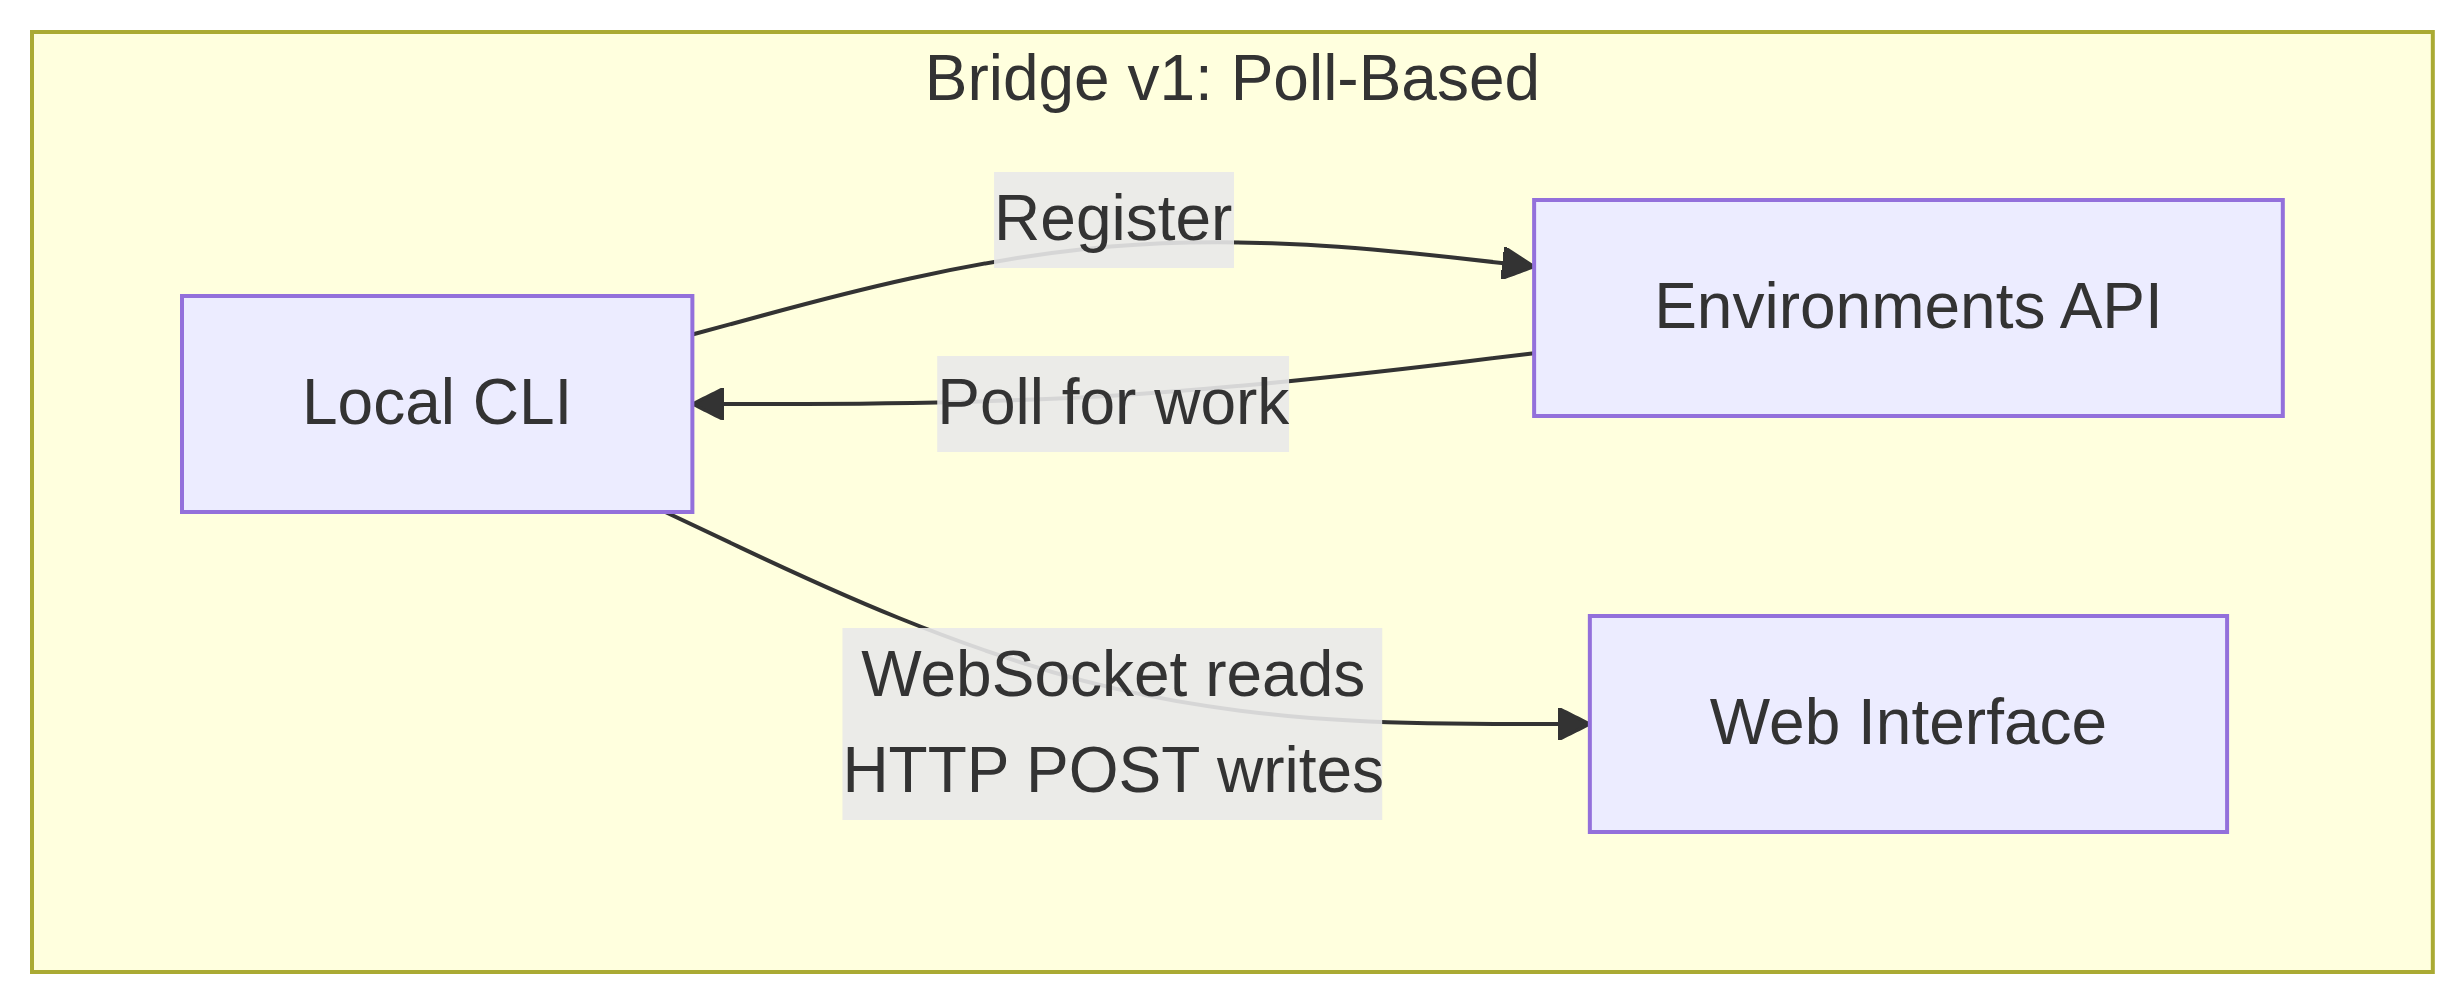
\includegraphics[width=6.42in,height=2.61in]{book/ch16-remote_files/figure-latex/mermaid-figure-1.png}

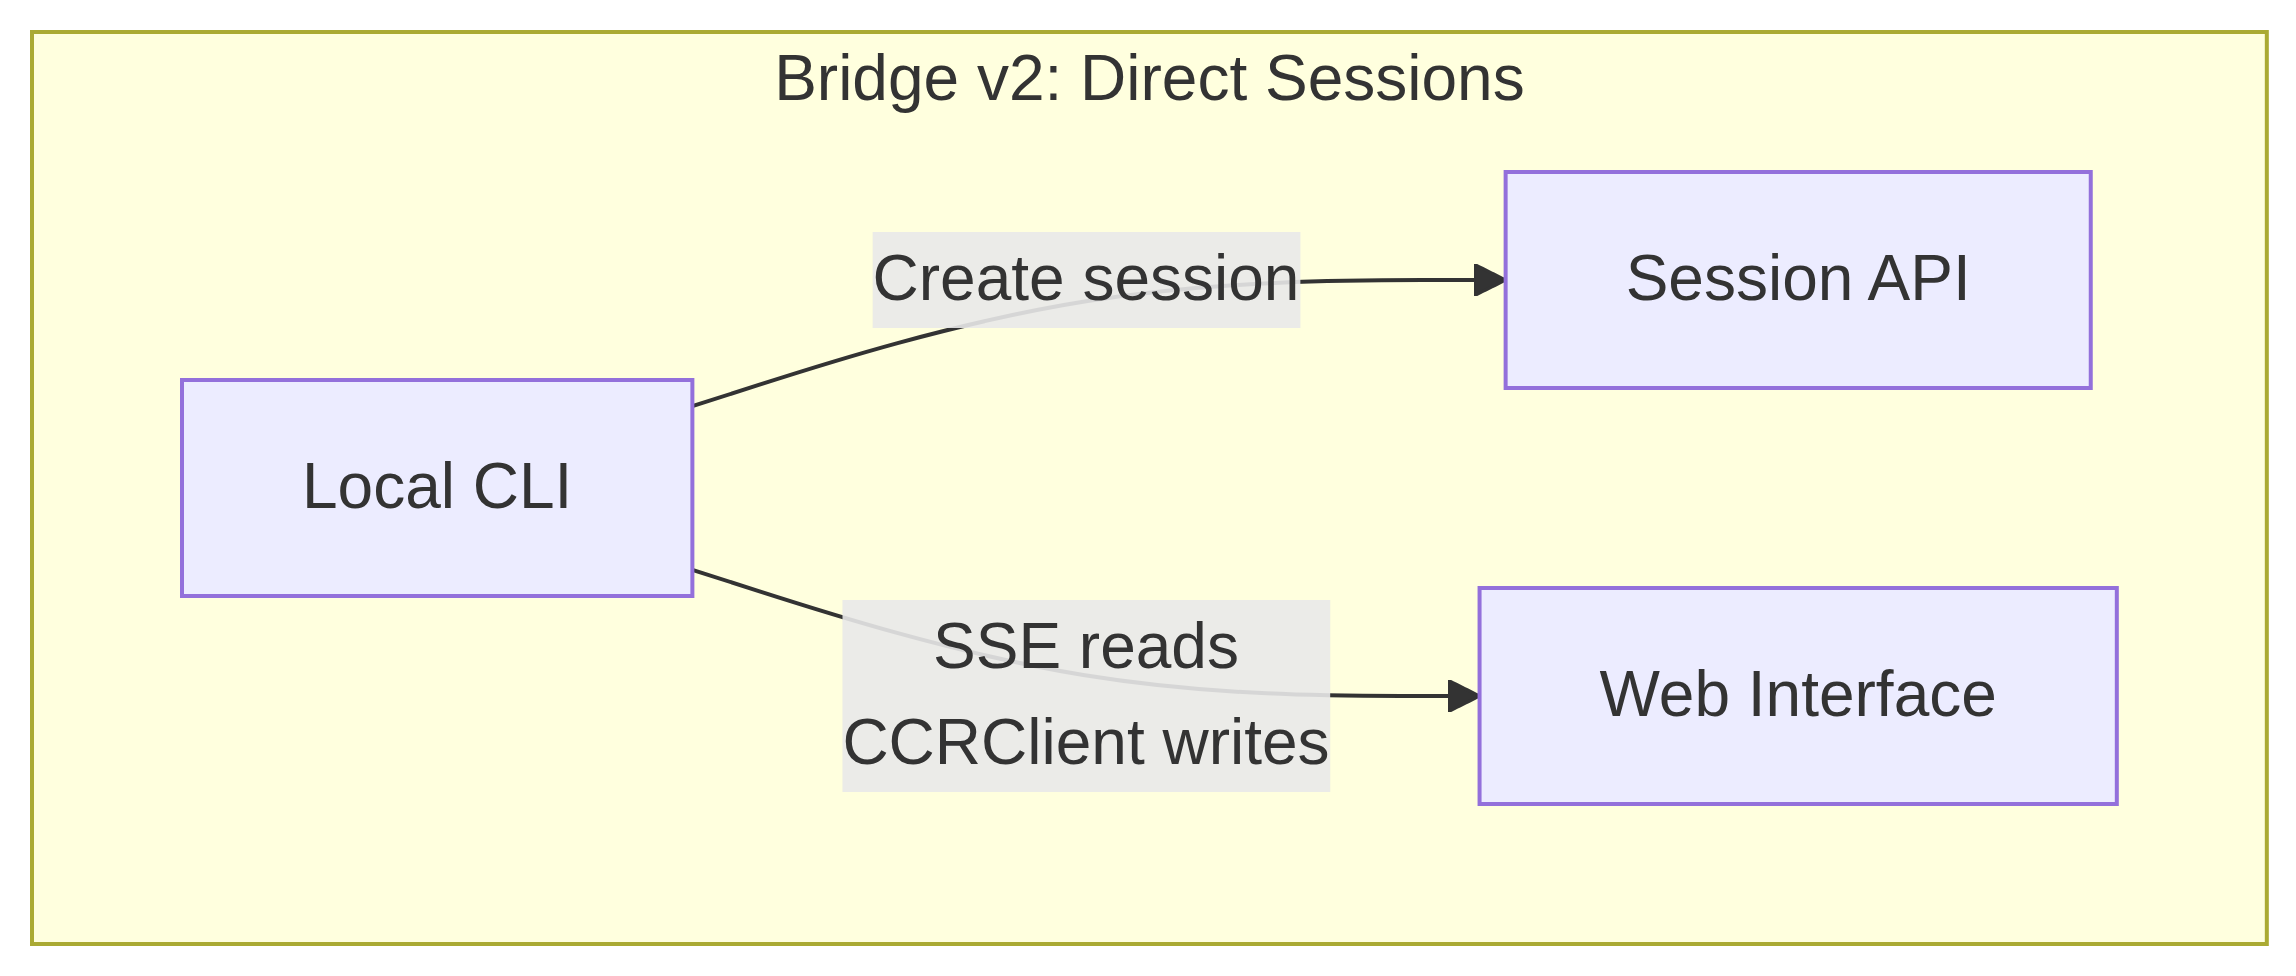
\includegraphics[width=5.99in,height=2.54in]{book/ch16-remote_files/figure-latex/mermaid-figure-4.png}

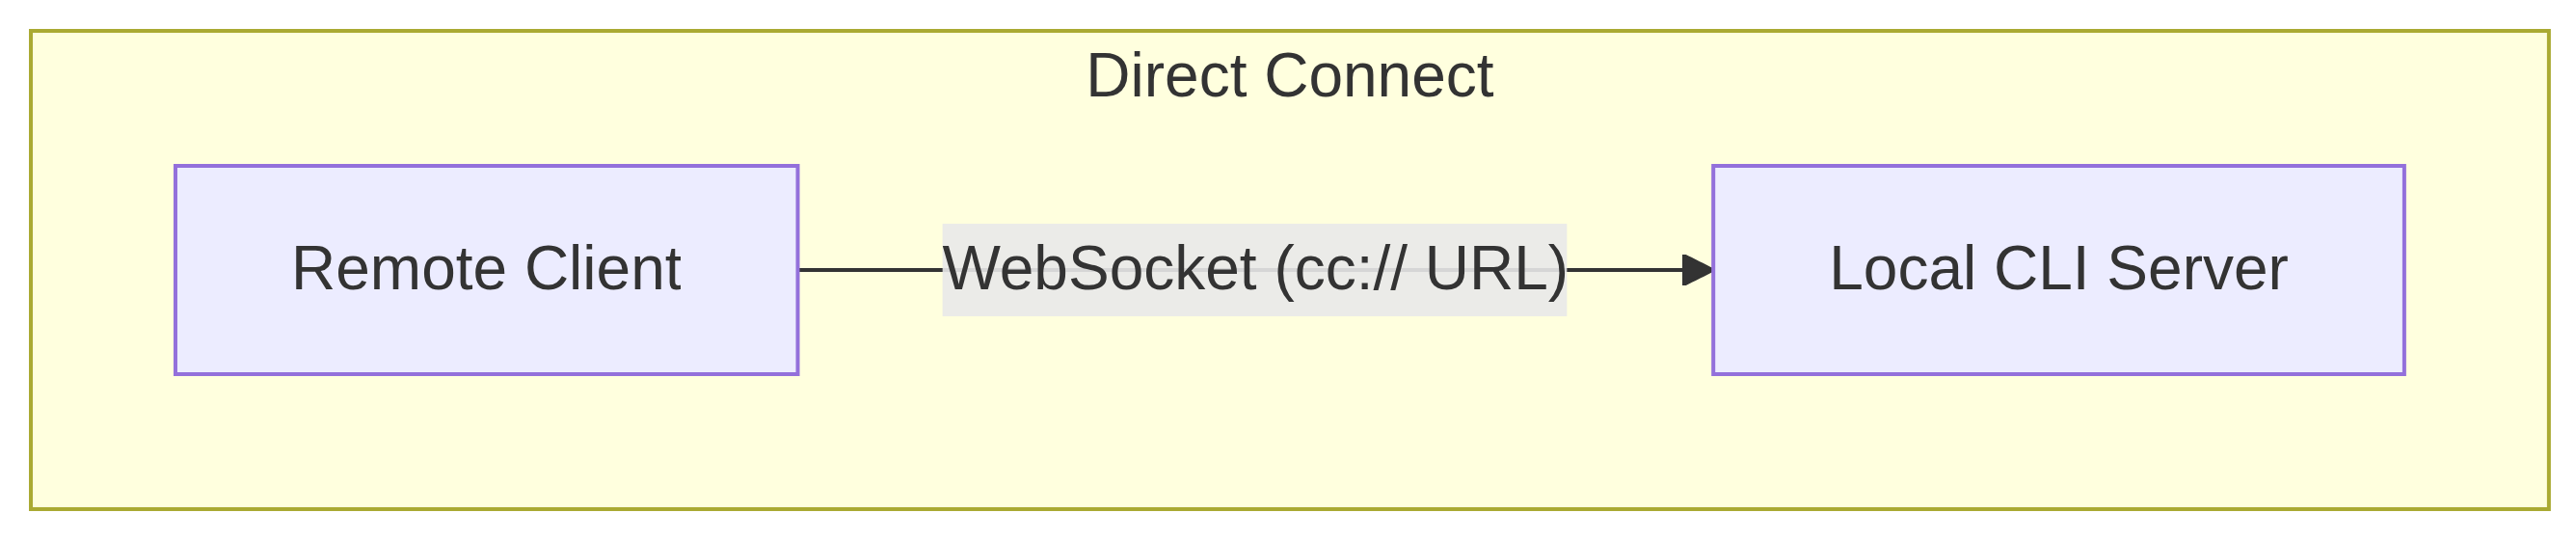
\includegraphics[width=6.97in,height=1.46in]{book/ch16-remote_files/figure-latex/mermaid-figure-3.png}

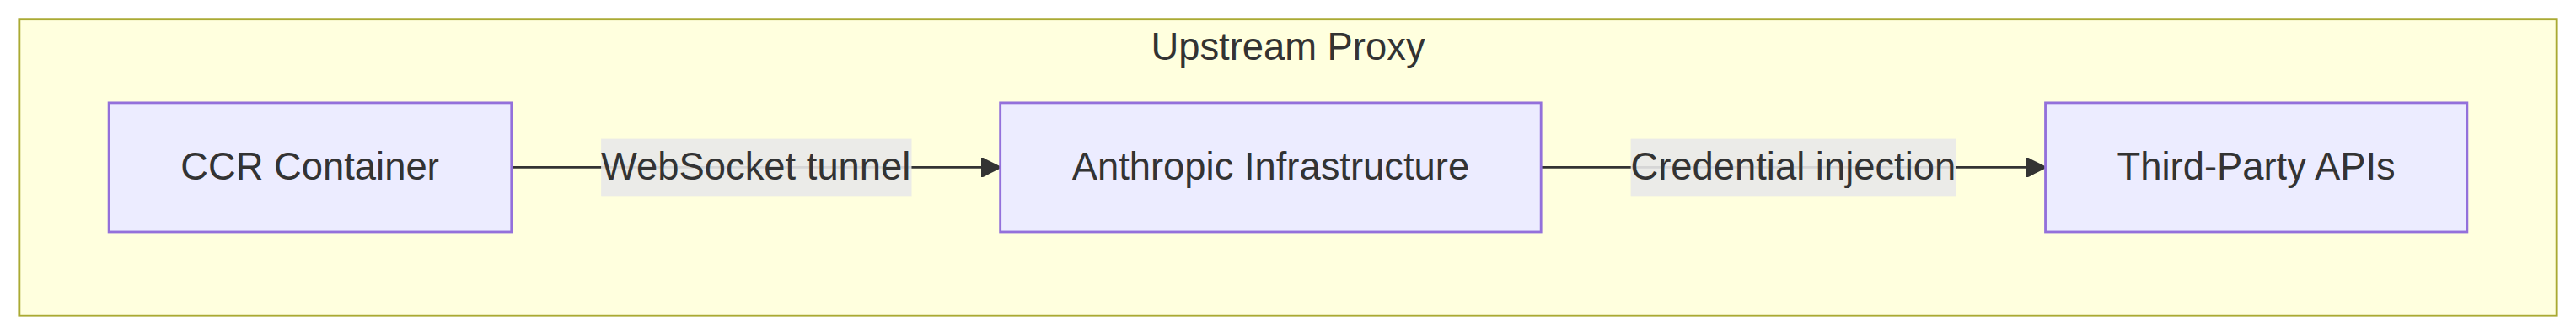
\includegraphics[width=11.23in,height=1.46in]{book/ch16-remote_files/figure-latex/mermaid-figure-2.png}

These systems share a common design philosophy: reads and writes are
asymmetric, reconnection is automatic, and failures degrade gracefully.

\begin{center}\rule{0.5\linewidth}{0.5pt}\end{center}

\section{Bridge v1: Poll, Dispatch,
Spawn}\label{bridge-v1-poll-dispatch-spawn}

The v1 bridge is the environment-based remote control system. When a
developer runs \texttt{claude\ remote-control}, the CLI registers with
the Environments API, polls for work, and spawns a child process per
session.

Before registration, a gauntlet of pre-flight checks runs: runtime
feature gate, OAuth token validation, organization policy check, dead
token detection (a cross-process backoff after three consecutive
failures with the same expired token), and proactive token refresh that
eliminates roughly 9\% of registrations that would otherwise fail on the
first attempt.

Once registered, the bridge enters a long-poll loop. Work items arrive
as sessions (with a \texttt{secret} field containing session tokens, API
base URL, MCP configs, and environment variables) or healthchecks. The
bridge throttles ``no work'' log messages to every 100 empty polls.

Each session spawns a child Claude Code process communicating via NDJSON
on stdin/stdout. Permission requests flow through the bridge transport
to the web interface where the user approves or denies. The round-trip
must complete within roughly 10-14 seconds.

\begin{center}\rule{0.5\linewidth}{0.5pt}\end{center}

\section{Bridge v2: Direct Sessions and
SSE}\label{bridge-v2-direct-sessions-and-sse}

The v2 bridge eliminates the entire Environments API layer -- no
registration, no polling, no acknowledgment, no heartbeat, no
deregistration. The motivation: v1 required the server to know the
machine's capabilities before dispatching work. V2 collapses the
lifecycle to three steps:

\begin{enumerate}
\def\labelenumi{\arabic{enumi}.}
\tightlist
\item
  \textbf{Create session}: \texttt{POST\ /v1/code/sessions} with OAuth
  credentials.
\item
  \textbf{Connect bridge}:
  \texttt{POST\ /v1/code/sessions/\{id\}/bridge}. Returns a
  \texttt{worker\_jwt}, \texttt{api\_base\_url}, and
  \texttt{worker\_epoch}. Each \texttt{/bridge} call bumps the epoch --
  it IS the registration.
\item
  \textbf{Open transport}: SSE for reads, \texttt{CCRClient} for writes.
\end{enumerate}

The transport abstraction (\texttt{ReplBridgeTransport}) unifies v1 and
v2 behind a common interface, so message handling does not need to know
which generation it is talking to.

When the SSE connection drops due to a 401, the transport rebuilds with
fresh credentials from a new \texttt{/bridge} call while preserving the
sequence number cursor -- no messages are lost. The write path uses
per-instance \texttt{getAuthToken} closures instead of process-wide
environment variables, preventing JWT leakage across concurrent
sessions.

\subsection{The FlushGate}\label{the-flushgate}

A subtle ordering problem: the bridge needs to send conversation history
while accepting live writes from the web interface. If a live write
arrives during the history flush, messages could be delivered out of
order. The \texttt{FlushGate} queues live writes during the flush POST
and drains them in order when it completes.

\subsection{Token Refresh and Epoch
Management}\label{token-refresh-and-epoch-management}

The v2 bridge proactively refreshes worker JWTs before expiry. A new
epoch tells the server this is the same worker with fresh credentials.
Epoch mismatches (409 responses) are handled aggressively: both
connections close and an exception unwinds the caller, preventing
split-brain scenarios.

\begin{center}\rule{0.5\linewidth}{0.5pt}\end{center}

\section{Message Routing and Echo
Deduplication}\label{message-routing-and-echo-deduplication}

Both bridge generations share \texttt{handleIngressMessage()} as the
central router:

\begin{enumerate}
\def\labelenumi{\arabic{enumi}.}
\tightlist
\item
  Parse JSON, normalize control message keys.
\item
  Route \texttt{control\_response} to permission handler,
  \texttt{control\_request} to request handler.
\item
  Check UUID against \texttt{recentPostedUUIDs} (echo dedup) and
  \texttt{recentInboundUUIDs} (re-delivery dedup).
\item
  Forward validated user messages.
\end{enumerate}

\subsection{BoundedUUIDSet: O(1) Lookup, O(capacity)
Memory}\label{boundeduuidset-o1-lookup-ocapacity-memory}

The bridge has an echo problem -- messages may echo back on the read
stream or be delivered twice during transport switches.
\texttt{BoundedUUIDSet} is a FIFO-bounded set backed by a circular
buffer:

\begin{Shaded}
\begin{Highlighting}[]
\KeywordTok{class}\NormalTok{ BoundedUUIDSet \{}
  \KeywordTok{private}\NormalTok{ buffer}\OperatorTok{:} \DataTypeTok{string}\NormalTok{[]}
  \KeywordTok{private} \KeywordTok{set}\OperatorTok{:} \BuiltInTok{Set}\OperatorTok{\textless{}}\DataTypeTok{string}\OperatorTok{\textgreater{}}
  \KeywordTok{private}\NormalTok{ head }\OperatorTok{=} \DecValTok{0}

  \FunctionTok{add}\NormalTok{(uuid}\OperatorTok{:} \DataTypeTok{string}\NormalTok{)}\OperatorTok{:} \DataTypeTok{void}\NormalTok{ \{}
    \ControlFlowTok{if}\NormalTok{ (}\KeywordTok{this}\OperatorTok{.}\AttributeTok{set}\OperatorTok{.}\AttributeTok{size} \OperatorTok{\textgreater{}=} \KeywordTok{this}\OperatorTok{.}\AttributeTok{capacity}\NormalTok{) \{}
      \KeywordTok{this}\OperatorTok{.}\AttributeTok{set}\OperatorTok{.}\FunctionTok{delete}\NormalTok{(}\KeywordTok{this}\OperatorTok{.}\AttributeTok{buffer}\NormalTok{[}\KeywordTok{this}\OperatorTok{.}\AttributeTok{head}\NormalTok{])}
\NormalTok{    \}}
    \KeywordTok{this}\OperatorTok{.}\AttributeTok{buffer}\NormalTok{[}\KeywordTok{this}\OperatorTok{.}\AttributeTok{head}\NormalTok{] }\OperatorTok{=}\NormalTok{ uuid}
    \KeywordTok{this}\OperatorTok{.}\AttributeTok{set}\OperatorTok{.}\FunctionTok{add}\NormalTok{(uuid)}
    \KeywordTok{this}\OperatorTok{.}\AttributeTok{head} \OperatorTok{=}\NormalTok{ (}\KeywordTok{this}\OperatorTok{.}\AttributeTok{head} \OperatorTok{+} \DecValTok{1}\NormalTok{) }\OperatorTok{\%} \KeywordTok{this}\OperatorTok{.}\AttributeTok{capacity}
\NormalTok{  \}}

  \FunctionTok{has}\NormalTok{(uuid}\OperatorTok{:} \DataTypeTok{string}\NormalTok{)}\OperatorTok{:} \DataTypeTok{boolean}\NormalTok{ \{ }\ControlFlowTok{return} \KeywordTok{this}\OperatorTok{.}\AttributeTok{set}\OperatorTok{.}\FunctionTok{has}\NormalTok{(uuid) \}}
\NormalTok{\}}
\end{Highlighting}
\end{Shaded}

Two instances run in parallel, each with capacity 2000. O(1) lookup via
the Set, O(capacity) memory via circular buffer eviction, no timers or
TTLs. Unknown control request subtypes get an error response, not
silence -- preventing the server from waiting for a response that never
comes.

\begin{center}\rule{0.5\linewidth}{0.5pt}\end{center}

\section{The Asymmetric Design: Persistent Reads, HTTP POST
Writes}\label{the-asymmetric-design-persistent-reads-http-post-writes}

The CCR protocol uses asymmetric transport: reads flow through a
persistent connection (WebSocket or SSE), writes go through HTTP POST.
This reflects a fundamental asymmetry in the communication pattern.

Reads are high-frequency, low-latency, server-initiated -- hundreds of
small messages per second during token streaming. A persistent
connection is the only sensible choice. Writes are low-frequency,
client-initiated, and require acknowledgment -- messages per minute, not
per second. HTTP POST provides reliable delivery, idempotency via UUIDs,
and natural integration with load balancers.

Trying to unify them on a single WebSocket creates coupling: if the
WebSocket drops during a write, you need retry logic and must
distinguish ``not sent'' from ``sent but acknowledgment lost.'' Separate
channels let each be optimized independently.

\begin{center}\rule{0.5\linewidth}{0.5pt}\end{center}

\section{Remote Session Management}\label{remote-session-management}

The \texttt{SessionsWebSocket} manages the client side of a CCR
WebSocket connection. Its reconnection strategy discriminates between
failure types:

\begin{longtable}[]{@{}
  >{\raggedright\arraybackslash}p{(\linewidth - 2\tabcolsep) * \real{0.4737}}
  >{\raggedright\arraybackslash}p{(\linewidth - 2\tabcolsep) * \real{0.5263}}@{}}
\toprule\noalign{}
\begin{minipage}[b]{\linewidth}\raggedright
Failure
\end{minipage} & \begin{minipage}[b]{\linewidth}\raggedright
Strategy
\end{minipage} \\
\midrule\noalign{}
\endhead
\bottomrule\noalign{}
\endlastfoot
4003 (unauthorized) & Stop immediately, no retries \\
4001 (session not found) & Max 3 retries, linear backoff (transient
during compaction) \\
Other transient & Exponential backoff, max 5 attempts \\
\end{longtable}

The \texttt{isSessionsMessage()} type guard accepts any object with a
string \texttt{type} field -- deliberately permissive. A hardcoded
allowlist would silently drop new message types before the client is
updated.

\begin{center}\rule{0.5\linewidth}{0.5pt}\end{center}

\section{Direct Connect: The Local
Server}\label{direct-connect-the-local-server}

Direct Connect is the simplest topology: Claude Code runs as a server
and clients connect via WebSocket. No cloud intermediary, no OAuth
tokens.

Sessions have five states: \texttt{starting}, \texttt{running},
\texttt{detached}, \texttt{stopping}, \texttt{stopped}. Metadata
persists to \texttt{\textasciitilde{}/.claude/server-sessions.json} for
resume across server restarts. The \texttt{cc://} URL scheme provides
clean addressing for local connections.

\begin{center}\rule{0.5\linewidth}{0.5pt}\end{center}

\section{Upstream Proxy: Credential Injection in
Containers}\label{upstream-proxy-credential-injection-in-containers}

The upstream proxy runs inside CCR containers and solves a specific
problem: injecting organization credentials into outbound HTTPS traffic
from a container where the agent might execute untrusted commands.

The setup sequence is carefully ordered:

\begin{enumerate}
\def\labelenumi{\arabic{enumi}.}
\tightlist
\item
  Read the session token from \texttt{/run/ccr/session\_token}.
\item
  Set \texttt{prctl(PR\_SET\_DUMPABLE,\ 0)} via Bun FFI -- blocking
  same-UID ptrace of the process heap. Without this, a prompt-injected
  \texttt{gdb\ -p\ \$PPID} could scrape the token from memory.
\item
  Download the upstream proxy CA certificate and concatenate with system
  CA bundle.
\item
  Start a local CONNECT-to-WebSocket relay on an ephemeral port.
\item
  Unlink the token file -- the token now exists only on the heap.
\item
  Export environment variables for all subprocesses.
\end{enumerate}

Every step fails open: errors disable the proxy rather than killing the
session. The correct tradeoff -- a failed proxy means some integrations
will not work, but core functionality remains available.

\subsection{Protobuf Hand-Encoding}\label{protobuf-hand-encoding}

Bytes through the tunnel are wrapped in \texttt{UpstreamProxyChunk}
protobuf messages. The schema is trivial --
\texttt{message\ UpstreamProxyChunk\ \{\ bytes\ data\ =\ 1;\ \}} -- and
Claude Code encodes it by hand in ten lines rather than pulling in a
protobuf runtime:

\begin{Shaded}
\begin{Highlighting}[]
\ImportTok{export} \KeywordTok{function} \FunctionTok{encodeChunk}\NormalTok{(data}\OperatorTok{:} \BuiltInTok{Uint8Array}\NormalTok{)}\OperatorTok{:} \BuiltInTok{Uint8Array}\NormalTok{ \{}
  \KeywordTok{const}\NormalTok{ varint}\OperatorTok{:} \DataTypeTok{number}\NormalTok{[] }\OperatorTok{=}\NormalTok{ []}
  \KeywordTok{let}\NormalTok{ n }\OperatorTok{=}\NormalTok{ data}\OperatorTok{.}\AttributeTok{length}
  \ControlFlowTok{while}\NormalTok{ (n }\OperatorTok{\textgreater{}} \BaseNTok{0x7f}\NormalTok{) \{ varint}\OperatorTok{.}\FunctionTok{push}\NormalTok{((n }\OperatorTok{\&} \BaseNTok{0x7f}\NormalTok{) }\OperatorTok{|} \BaseNTok{0x80}\NormalTok{)}\OperatorTok{;}\NormalTok{ n }\OperatorTok{\textgreater{}\textgreater{}\textgreater{}=} \DecValTok{7}\NormalTok{ \}}
\NormalTok{  varint}\OperatorTok{.}\FunctionTok{push}\NormalTok{(n)}
  \KeywordTok{const}\NormalTok{ out }\OperatorTok{=} \KeywordTok{new} \BuiltInTok{Uint8Array}\NormalTok{(}\DecValTok{1} \OperatorTok{+}\NormalTok{ varint}\OperatorTok{.}\AttributeTok{length} \OperatorTok{+}\NormalTok{ data}\OperatorTok{.}\AttributeTok{length}\NormalTok{)}
\NormalTok{  out[}\DecValTok{0}\NormalTok{] }\OperatorTok{=} \BaseNTok{0x0a}  \CommentTok{// field 1, wire type 2}
\NormalTok{  out}\OperatorTok{.}\FunctionTok{set}\NormalTok{(varint}\OperatorTok{,} \DecValTok{1}\NormalTok{)}
\NormalTok{  out}\OperatorTok{.}\FunctionTok{set}\NormalTok{(data}\OperatorTok{,} \DecValTok{1} \OperatorTok{+}\NormalTok{ varint}\OperatorTok{.}\AttributeTok{length}\NormalTok{)}
  \ControlFlowTok{return}\NormalTok{ out}
\NormalTok{\}}
\end{Highlighting}
\end{Shaded}

Ten lines replace a full protobuf runtime. A single-field message does
not justify a dependency -- the maintenance burden of the bit
manipulation is far lower than the supply chain risk.

\begin{center}\rule{0.5\linewidth}{0.5pt}\end{center}

\section{Apply This: Designing Remote Agent
Execution}\label{apply-this-designing-remote-agent-execution}

\textbf{Separate read and write channels.} When reads are high-frequency
streams and writes are low-frequency RPCs, unifying them creates
unnecessary coupling. Let each channel fail and recover independently.

\textbf{Bound your deduplication memory.} The BoundedUUIDSet pattern
provides fixed-memory deduplication. Any at-least-once delivery system
needs a bounded dedup buffer, not an unbounded Set.

\textbf{Make reconnection strategy proportional to the failure signal.}
Permanent failures should not retry. Transient failures should retry
with backoff. Ambiguous failures should retry with a low cap.

\textbf{Keep secrets heap-only in adversarial environments.} Reading the
token from a file, disabling ptrace, and unlinking the file eliminates
both filesystem and memory-inspection attack vectors.

\textbf{Fail open for auxiliary systems.} The upstream proxy fails open
because it provides enhanced functionality (credential injection), not
core functionality (model inference).

The remote execution systems encode a deeper principle: the agent's core
loop (Chapter 5) should be agnostic about where instructions come from
and where results go. The bridge, Direct Connect, and upstream proxy are
transport layers. The message handling, tool execution, and permission
flows above them are identical regardless of whether the user is sitting
at the terminal or on the other side of a WebSocket.

The next chapter examines the other operational concern: performance --
how Claude Code makes every millisecond and token count across startup,
rendering, search, and API costs.

\part{Part VII: Performance Engineering}

\chapter{Chapter 17: Performance -- Every Millisecond and Token
Counts}\label{chapter-17-performance-every-millisecond-and-token-counts}

\section{The Senior Engineer's
Playbook}\label{the-senior-engineers-playbook}

Performance optimization in an agentic system is not one problem. It is
five:

\begin{enumerate}
\def\labelenumi{\arabic{enumi}.}
\tightlist
\item
  \textbf{Startup latency} -- the time from keystroke to first useful
  output. Users abandon tools that feel slow to launch.
\item
  \textbf{Token efficiency} -- the fraction of the context window
  consumed by useful content versus overhead. The context window is the
  most constrained resource.
\item
  \textbf{API cost} -- the dollar amount per turn. Prompt caching can
  reduce this by 90\%, but only if the system preserves cache stability
  across turns.
\item
  \textbf{Rendering throughput} -- the frames per second during
  streaming output. Chapter 13 covered the rendering architecture; this
  chapter covers the performance measurements and optimizations that
  keep it fast.
\item
  \textbf{Search speed} -- the time to find a file in a 270,000-path
  codebase on every keystroke.
\end{enumerate}

Claude Code attacks all five with techniques ranging from the obvious
(memoization) to the subtle (26-bit bitmaps for pre-filtering fuzzy
search). A note on methodology: these are not theoretical optimizations.
Claude Code ships with 50+ startup profiling checkpoints, sampled at
100\% of internal users and 0.5\% of external users. Every optimization
below was motivated by data from this instrumentation, not by intuition.

\begin{center}\rule{0.5\linewidth}{0.5pt}\end{center}

\section{Saving Milliseconds at
Startup}\label{saving-milliseconds-at-startup}

\subsection{Module-Level I/O
Parallelism}\label{module-level-io-parallelism}

The entry point \texttt{main.tsx} deliberately violates ``no side
effects at module scope'':

\begin{Shaded}
\begin{Highlighting}[]
\FunctionTok{profileCheckpoint}\NormalTok{(}\StringTok{\textquotesingle{}main\_tsx\_entry\textquotesingle{}}\NormalTok{)}\OperatorTok{;}
\FunctionTok{startMdmRawRead}\NormalTok{()}\OperatorTok{;}       \CommentTok{// fires plutil/reg{-}query subprocesses}
\FunctionTok{startKeychainPrefetch}\NormalTok{()}\OperatorTok{;}  \CommentTok{// fires both macOS keychain reads in parallel}
\end{Highlighting}
\end{Shaded}

Two macOS keychain entries would otherwise cost \textasciitilde65ms of
sequential synchronous spawns. By launching both as fire-and-forget
promises at the module level, they execute in parallel with
\textasciitilde135ms of module loading during which the CPU would
otherwise be idle.

\subsection{API Preconnection}\label{api-preconnection}

\texttt{apiPreconnect.ts} fires a \texttt{HEAD} request to the Anthropic
API during initialization, overlapping the TCP+TLS handshake (100-200ms)
with setup work. In interactive mode, the overlap is unbounded -- the
connection warms while the user types. The request fires after
\texttt{applyExtraCACertsFromConfig()} and
\texttt{configureGlobalAgents()} so the warmed connection uses the
correct transport configuration.

\subsection{Fast-Path Dispatch and Deferred
Imports}\label{fast-path-dispatch-and-deferred-imports}

The CLI entry point contains early-return paths for specialized
subcommands -- \texttt{claude\ mcp} never loads the React REPL,
\texttt{claude\ daemon} never loads the tool system. Heavy modules are
loaded via dynamic \texttt{import()} only when needed: OpenTelemetry
(\textasciitilde400KB + \textasciitilde700KB gRPC), event logging, error
dialogs, upstream proxy. \texttt{LazySchema} defers Zod schema
construction to first validation, pushing the cost past startup.

\begin{center}\rule{0.5\linewidth}{0.5pt}\end{center}

\section{Saving Tokens in the Context
Window}\label{saving-tokens-in-the-context-window}

\subsection{Slot Reservation: 8K Default, 64K
Escalation}\label{slot-reservation-8k-default-64k-escalation}

The most impactful single optimization:

The default output slot reservation is 8,000 tokens, escalating to
64,000 on truncation. The API reserves \texttt{max\_output\_tokens} of
capacity for the model's response. The default SDK value is 32K-64K, but
production data shows p99 output length is 4,911 tokens. The default
over-reserves by 8-16x, wasting 24,000-59,000 tokens per turn. Claude
Code caps at 8K and retries at 64K on the rare truncation (\textless1\%
of requests). For a 200K window, this is a 12-28\% improvement in usable
context -- for free.

\subsection{Tool Result Budgeting}\label{tool-result-budgeting}

\begin{longtable}[]{@{}
  >{\raggedright\arraybackslash}p{(\linewidth - 4\tabcolsep) * \real{0.3043}}
  >{\raggedright\arraybackslash}p{(\linewidth - 4\tabcolsep) * \real{0.3043}}
  >{\raggedright\arraybackslash}p{(\linewidth - 4\tabcolsep) * \real{0.3913}}@{}}
\toprule\noalign{}
\begin{minipage}[b]{\linewidth}\raggedright
Limit
\end{minipage} & \begin{minipage}[b]{\linewidth}\raggedright
Value
\end{minipage} & \begin{minipage}[b]{\linewidth}\raggedright
Purpose
\end{minipage} \\
\midrule\noalign{}
\endhead
\bottomrule\noalign{}
\endlastfoot
Per-tool characters & 50,000 & Results persisted to disk when
exceeded \\
Per-tool tokens & 100,000 & \textasciitilde400KB text upper bound \\
Per-message aggregate & 200,000 chars & Prevents N parallel tools from
blowing the budget in one turn \\
\end{longtable}

The per-message aggregate is the key insight. Without it, ``read all
files in src/'' could produce 10 parallel reads each returning 40K
characters.

\subsection{Context Window Sizing}\label{context-window-sizing}

The default 200K-token window is expandable to 1M via the
\texttt{{[}1m{]}} suffix on model names or experiment treatment. When
usage approaches the limit, a 4-layer compaction system progressively
summarizes older content. Token counting is anchored on the API's actual
\texttt{usage} field, not client-side estimation -- accounting for
prompt caching credits, thinking tokens, and server-side
transformations.

\begin{center}\rule{0.5\linewidth}{0.5pt}\end{center}

\section{Saving Money on API Calls}\label{saving-money-on-api-calls}

\subsection{The Prompt Cache
Architecture}\label{the-prompt-cache-architecture}

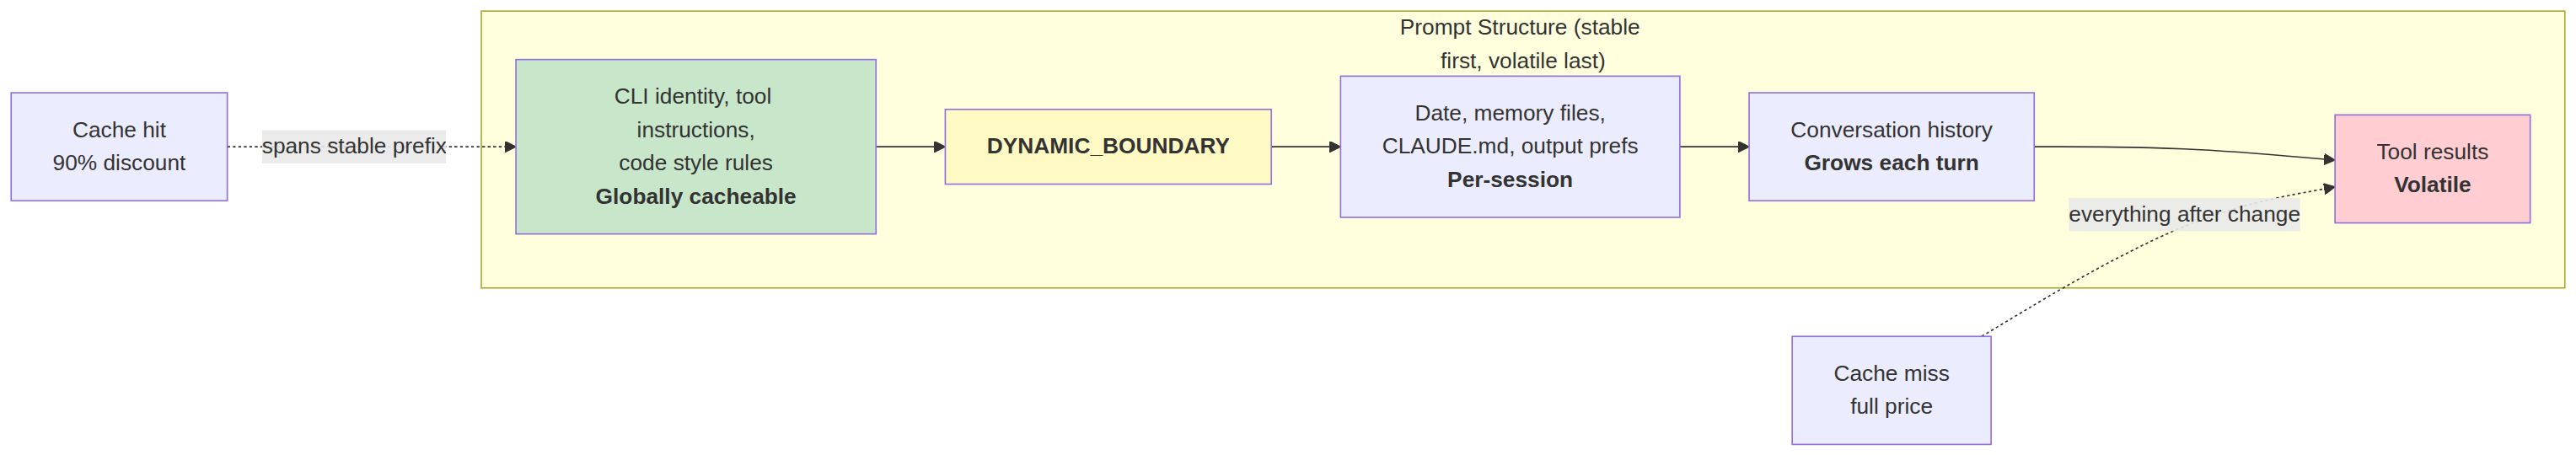
\includegraphics[width=19.37in,height=3.43in]{book/ch17-performance_files/figure-latex/mermaid-figure-1.png}

Anthropic's prompt cache operates on exact prefix matching. If a single
token changes mid-prefix, everything after is a cache miss. Claude Code
structures the entire prompt so stable parts come first and volatile
parts come last.

When \texttt{shouldUseGlobalCacheScope()} returns true, system prompt
entries before the dynamic boundary get
\texttt{scope:\ \textquotesingle{}global\textquotesingle{}} -- two users
running the same Claude Code version share the prefix cache. Global
scope is disabled when MCP tools are present, since MCP schemas are
per-user.

\subsection{Sticky Latch Fields}\label{sticky-latch-fields}

Five boolean fields use a ``sticky-on'' pattern -- once true, they
remain true for the session:

\begin{longtable}[]{@{}
  >{\raggedright\arraybackslash}p{(\linewidth - 2\tabcolsep) * \real{0.4333}}
  >{\raggedright\arraybackslash}p{(\linewidth - 2\tabcolsep) * \real{0.5667}}@{}}
\toprule\noalign{}
\begin{minipage}[b]{\linewidth}\raggedright
Latch Field
\end{minipage} & \begin{minipage}[b]{\linewidth}\raggedright
What It Prevents
\end{minipage} \\
\midrule\noalign{}
\endhead
\bottomrule\noalign{}
\endlastfoot
\texttt{promptCache1hEligible} & Mid-session overage flip changing cache
TTL \\
\texttt{afkModeHeaderLatched} & Shift+Tab toggles busting cache \\
\texttt{fastModeHeaderLatched} & Cooldown enter/exit double-busting
cache \\
\texttt{cacheEditingHeaderLatched} & Mid-session config toggles busting
cache \\
\texttt{thinkingClearLatched} & Flipping thinking mode after confirmed
cache miss \\
\end{longtable}

Each corresponds to a header or parameter that, if changed mid-session,
would bust \textasciitilde50,000-70,000 tokens of cached prompt. The
latches sacrifice mid-session toggling to preserve the cache.

\subsection{Memoized Session Date}\label{memoized-session-date}

\begin{Shaded}
\begin{Highlighting}[]
\KeywordTok{const}\NormalTok{ getSessionStartDate }\OperatorTok{=} \FunctionTok{memoize}\NormalTok{(getLocalISODate)}
\end{Highlighting}
\end{Shaded}

Without this, the date would change at midnight, busting the entire
cached prefix. A stale date is cosmetic; a cache bust reprocesses the
entire conversation.

\subsection{Section Memoization}\label{section-memoization}

System prompt sections use a two-tier cache. Most content uses
\texttt{systemPromptSection(name,\ compute)}, cached until
\texttt{/clear} or \texttt{/compact}. The nuclear option
\texttt{DANGEROUS\_uncachedSystemPromptSection(name,\ compute,\ reason)}
recomputes every turn -- the naming convention forces developers to
document WHY cache-breaking is necessary.

\begin{center}\rule{0.5\linewidth}{0.5pt}\end{center}

\section{Saving CPU in Rendering}\label{saving-cpu-in-rendering}

Chapter 13 covered the rendering architecture in depth -- the packed
typed arrays, pool-based interning, double buffering, and cell-level
diffing. Here we focus on the performance measurements and adaptive
behaviors that keep it fast.

The terminal renderer throttles at 60fps via
\texttt{throttle(deferredRender,\ FRAME\_INTERVAL\_MS)}. When the
terminal is blurred, the interval doubles to 30fps. Scroll drain frames
run at quarter interval for maximum scroll speed. This adaptive
throttling ensures rendering never consumes more CPU than necessary.

The React Compiler (\texttt{react/compiler-runtime}) auto-memoizes
component renders throughout the codebase. Manual \texttt{useMemo} and
\texttt{useCallback} are error-prone; the compiler gets it right by
construction. Pre-allocated frozen objects (\texttt{Object.freeze()})
eliminate allocations for common render-path values -- one allocation
saved per frame in alt-screen mode compounds over thousands of frames.

For the full rendering pipeline details -- the
\texttt{CharPool}/\texttt{StylePool}/\texttt{HyperlinkPool} interning
system, the blit optimization, the damage rectangle tracking, the
OffscreenFreeze component -- see Chapter 13.

\begin{center}\rule{0.5\linewidth}{0.5pt}\end{center}

\section{Saving Memory and Time in
Search}\label{saving-memory-and-time-in-search}

The fuzzy file search runs on every keystroke, searching 270,000+ paths.
Three optimization layers keep it under a few milliseconds.

\subsection{The Bitmap Pre-Filter}\label{the-bitmap-pre-filter}

Every indexed path gets a 26-bit bitmap of which lowercase letters it
contains:

\begin{Shaded}
\begin{Highlighting}[]
\CommentTok{// Pseudocode — illustrates the 26{-}bit bitmap concept}
\KeywordTok{function} \FunctionTok{buildCharBitmap}\NormalTok{(filepath}\OperatorTok{:} \DataTypeTok{string}\NormalTok{)}\OperatorTok{:} \DataTypeTok{number}\NormalTok{ \{}
  \KeywordTok{let}\NormalTok{ mask }\OperatorTok{=} \DecValTok{0}
  \ControlFlowTok{for}\NormalTok{ (}\KeywordTok{const}\NormalTok{ ch }\KeywordTok{of}\NormalTok{ filepath}\OperatorTok{.}\FunctionTok{toLowerCase}\NormalTok{()) \{}
    \KeywordTok{const}\NormalTok{ code }\OperatorTok{=}\NormalTok{ ch}\OperatorTok{.}\FunctionTok{charCodeAt}\NormalTok{(}\DecValTok{0}\NormalTok{)}
    \ControlFlowTok{if}\NormalTok{ (code }\OperatorTok{\textgreater{}=} \DecValTok{97} \OperatorTok{\&\&}\NormalTok{ code }\OperatorTok{\textless{}=} \DecValTok{122}\NormalTok{) mask }\OperatorTok{|=} \DecValTok{1} \OperatorTok{\textless{}\textless{}}\NormalTok{ (code }\OperatorTok{{-}} \DecValTok{97}\NormalTok{)}
\NormalTok{  \}}
  \ControlFlowTok{return}\NormalTok{ mask  }\CommentTok{// Each bit represents presence of a{-}z}
\NormalTok{\}}
\end{Highlighting}
\end{Shaded}

At search time:
\texttt{if\ ((charBits{[}i{]}\ \&\ needleBitmap)\ !==\ needleBitmap)\ continue}.
Any path missing a query letter fails instantly -- one integer
comparison, no string operations. Rejection rate: \textasciitilde10\%
for broad queries like ``test,'' 90\%+ for queries with rare letters.
Cost: 4 bytes per path, \textasciitilde1MB for 270,000 paths.

\subsection{Score-Bound Rejection and Fused indexOf
Scan}\label{score-bound-rejection-and-fused-indexof-scan}

Paths surviving the bitmap face a score ceiling check before the
expensive boundary/camelCase scoring. If the best-case score cannot beat
the current top-K threshold, the path is skipped.

The actual matching fuses position finding with gap/consecutive bonus
computation using \texttt{String.indexOf()}, which is SIMD-accelerated
in both JSC (Bun) and V8 (Node). The engine's optimized search is
significantly faster than manual character loops.

\subsection{Async Indexing with Partial
Queryability}\label{async-indexing-with-partial-queryability}

For large codebases, \texttt{loadFromFileListAsync()} yields to the
event loop every \textasciitilde4ms of work (time-based, not count-based
-- adapting to machine speed). It returns two promises:
\texttt{queryable} (resolves on first chunk, enabling immediate partial
results) and \texttt{done} (full index complete). The user can start
searching within 5-10ms of the file list becoming available.

The yield check uses \texttt{(i\ \&\ 0xff)\ ===\ 0xff} -- a branchless
modulo-256 to amortize the cost of \texttt{performance.now()}.

\begin{center}\rule{0.5\linewidth}{0.5pt}\end{center}

\section{The Memory Relevance
Side-Query}\label{the-memory-relevance-side-query}

One optimization sits at the intersection of token efficiency and API
cost. As described in Chapter 11, the memory system uses a lightweight
Sonnet model call -- not the main Opus model -- to select which memory
files to include. The cost (256 max output tokens on a fast model) is
negligible compared to the tokens saved by not including irrelevant
memory files. A single irrelevant 2,000-token memory costs more in
wasted context than the side query costs in API calls.

\begin{center}\rule{0.5\linewidth}{0.5pt}\end{center}

\section{Speculative Tool Execution}\label{speculative-tool-execution}

The \texttt{StreamingToolExecutor} begins executing tools as they stream
in, before the full response completes. Read-only tools (Glob, Grep,
Read) can execute in parallel; write tools require exclusive access. The
\texttt{partitionToolCalls()} function groups consecutive safe tools
into batches: {[}Read, Read, Grep, Edit, Read, Read{]} becomes three
batches -- {[}Read, Read, Grep{]} concurrent, {[}Edit{]} serial,
{[}Read, Read{]} concurrent.

Results are always yielded in the original tool order for deterministic
model reasoning. A sibling abort controller kills parallel subprocesses
when a Bash tool errors, preventing resource waste.

\begin{center}\rule{0.5\linewidth}{0.5pt}\end{center}

\section{Streaming and the Raw API}\label{streaming-and-the-raw-api}

Claude Code uses the raw streaming API instead of the SDK's
\texttt{BetaMessageStream} helper. The helper calls
\texttt{partialParse()} on every \texttt{input\_json\_delta} --
O(n\^{}2) in tool input length. Claude Code accumulates raw strings and
parses once when the block is complete.

A streaming watchdog (\texttt{CLAUDE\_STREAM\_IDLE\_TIMEOUT\_MS},
default 90 seconds) aborts and retries if no chunks arrive, with
fallback to non-streaming \texttt{messages.create()} on proxy failure.

\begin{center}\rule{0.5\linewidth}{0.5pt}\end{center}

\section{Apply This: Performance for Agentic
Systems}\label{apply-this-performance-for-agentic-systems}

\textbf{Audit your context window budget.} The gap between your
\texttt{max\_output\_tokens} reservation and your actual p99 output
length is wasted context. Set a tight default and escalate on
truncation.

\textbf{Design for cache stability.} Every field in your prompt is
stable or volatile. Put stable first, volatile last. Treat any
mid-conversation change to the stable prefix as a bug with a dollar
cost.

\textbf{Parallelize startup I/O.} Module loading is CPU-bound. Keychain
reads and network handshakes are I/O-bound. Launch I/O before imports.

\textbf{Use bitmap pre-filters for search.} A cheap pre-filter rejecting
10-90\% of candidates before expensive scoring is a significant win at 4
bytes per entry.

\textbf{Measure where it matters.} Claude Code has 50+ startup
checkpoints, sampled at 100\% internally and 0.5\% externally.
Performance work without measurement is guesswork.

\begin{center}\rule{0.5\linewidth}{0.5pt}\end{center}

A final observation: most of these optimizations are not algorithmically
sophisticated. Bitmap pre-filters, circular buffers, memoization,
interning -- these are CS fundamentals. The sophistication is in knowing
where to apply them. The startup profiler tells you where the
milliseconds are. The API usage field tells you where the tokens are.
The cache hit rate tells you where the money is. Measurement first,
optimization second, always.

\chapter{Chapter 18: What We Learned}\label{chapter-18-what-we-learned}

\section{Five Architectural Bets}\label{five-architectural-bets}

Claude Code is not the only agentic system. It is not the first. But it
made five architectural bets that distinguish it from the landscape of
agent frameworks, and after nearly two thousand files and seventeen
chapters, those bets deserve examination.

\subsection{Bet 1: The Generator Loop Over
Callbacks}\label{bet-1-the-generator-loop-over-callbacks}

Most agent frameworks give you a pipeline: define tools, register
handlers, let the framework orchestrate. The developer writes callbacks.
The framework decides when to call them.

Claude Code does the opposite. The \texttt{query()} function is an async
generator -- the developer owns the loop. The model streams a response,
the generator yields tool calls, the caller executes them, appends
results, and the generator loops. There is one function, one data flow,
one place where every interaction passes through. The 10 terminal states
and 7 continuation states of the generator's return type encode every
possible outcome. The loop is the system.

The bet was that a single generator function, even one that grew to
1,700 lines, would be more comprehensible than a distributed callback
graph. After studying the source, the bet paid off. When you want to
understand why a session ended, you look at one function. When you want
to add a new terminal state, you add one variant to one discriminated
union. The type system enforces exhaustive handling. A callback
architecture would scatter this logic across dozens of files, and the
interactions between callbacks would be implicit rather than visible in
the control flow.

\subsection{Bet 2: File-Based Memory Over
Databases}\label{bet-2-file-based-memory-over-databases}

Chapter 11 made the case in detail, but the architectural significance
extends beyond memory. The decision to use plain Markdown files instead
of SQLite, a vector database, or a cloud service was a bet on
transparency over capability. A database would support richer queries,
faster lookups, and transactional guarantees. Files provide none of
that. What files provide is trust.

A user who opens
\texttt{\textasciitilde{}/.claude/projects/myapp/memory/MEMORY.md} in
vim and sees exactly what the agent remembers about them has a
fundamentally different relationship with the system than a user who
must ask the agent ``what do you remember?'' and hope the answer is
complete. The file-based design makes the agent's knowledge state
externally observable, not just self-reported. This matters more than
query performance. The LLM-powered recall system compensates for the
storage simplicity with retrieval intelligence -- a Sonnet side-query
selecting five relevant memories from a manifest is more precise than
embedding similarity and requires zero infrastructure.

\subsection{Bet 3: Self-Describing Tools Over Central
Orchestrators}\label{bet-3-self-describing-tools-over-central-orchestrators}

Agent frameworks typically provide a tool registry: you describe your
tools in a central configuration, and the framework presents them to the
model. Claude Code's tools describe themselves. Each \texttt{Tool}
object carries its own name, description, input schema, prompt
contribution, concurrency safety flag, and execution logic. The tool
system's job is not to describe tools to the model -- it is to let tools
describe themselves.

This bet pays off in extensibility. MCP tools (Chapter 15) become
first-class citizens by implementing the same interface. A tool from an
MCP server and a built-in tool are indistinguishable to the model. The
system does not need a separate ``MCP tool adapter'' layer -- the
wrapping produces a standard \texttt{Tool} object, and from that point
forward, the existing tool pipeline handles it: permission checking,
concurrent execution, result budgeting, hook interception.

\subsection{Bet 4: Fork Agents for Cache
Sharing}\label{bet-4-fork-agents-for-cache-sharing}

Chapter 9 covered the fork mechanism: a sub-agent that starts with the
parent's full conversation in its context window, sharing the parent's
prompt cache. This is not a convenience optimization -- it is an
architectural bet that the cache sharing model is worth the complexity
of fork lifecycle management.

The alternative -- spawning a fresh agent with a summary of the
conversation -- is simpler but expensive. Every fresh agent pays the
full cost of processing its context from scratch. A forked agent gets
the parent's cached prefix for free (a 90\% discount on input tokens),
making it economical to spawn agents for small tasks: memory extraction,
code review, verification passes. The background memory extraction agent
(Chapter 11) runs after every query loop turn, and its cost is marginal
precisely because it shares the parent's cache. Without fork-based cache
sharing, that agent would be prohibitively expensive.

\subsection{Bet 5: Hooks Over Plugins}\label{bet-5-hooks-over-plugins}

Most extensibility systems use plugins -- code that registers
capabilities and runs within the host process. Claude Code uses hooks --
external processes that run at lifecycle points and communicate through
exit codes and JSON on stdin/stdout.

The bet is that process isolation is worth the overhead. A plugin can
crash the host. A hook crashes its own process. A plugin can leak memory
into the host's heap. A hook's memory dies with its process. A plugin
requires an API surface that must be versioned and maintained. A hook
requires stdin, stdout, and an exit code -- a protocol that has been
stable since 1971.

The overhead is real: spawning a process per hook invocation costs
milliseconds that an in-process callback would not. The -70\% fast path
for internal callbacks (Chapter 12) shows that the system knows this
cost matters. But for external hooks -- user scripts, team linters,
enterprise policy servers -- the isolation guarantee makes the system
safer to extend. An enterprise can deploy hook-based policy enforcement
without worrying that a malformed hook script will crash their
developers' sessions.

\begin{center}\rule{0.5\linewidth}{0.5pt}\end{center}

\section{What Transfers, What Does
Not}\label{what-transfers-what-does-not}

Not every pattern in Claude Code generalizes. Some are consequences of
scale, resources, or specific constraints that other agent builders may
not share.

\subsection{Patterns That Transfer to Any
Agent}\label{patterns-that-transfer-to-any-agent}

\textbf{The generator loop pattern.} Any agent that needs to stream
responses, handle tool calls, and manage multiple terminal states
benefits from making the loop explicit rather than hiding it behind
callbacks. The discriminated union return type -- encoding exactly why
the loop stopped -- is a pattern that eliminates an entire class of
``why did the agent stop?'' debugging sessions.

\textbf{File-based memory with LLM recall.} The specific implementation
details are Claude Code's, but the principle -- simple storage combined
with intelligent retrieval -- applies to any agent that needs to persist
knowledge across sessions. The four-type taxonomy (user, feedback,
project, reference) and the derivability test (``can this be re-derived
from the current project state?'') are reusable design heuristics.

\textbf{Asymmetric read/write channels for remote execution.} When reads
are high-frequency streams and writes are low-frequency RPCs, separating
them is correct regardless of the specific transport protocol.

\textbf{Bitmap pre-filters for search.} Any agent searching a large file
index benefits from a 26-bit letter bitmap as a pre-filter. Four bytes
per entry, one integer comparison per candidate -- the cost-to-benefit
ratio is remarkable.

\textbf{Prompt cache stability as an architectural concern.} If your
agent uses an API with prompt caching, structuring the prompt with
stable content first and volatile content last is not an optimization --
it is an architectural decision that determines your cost structure.

\subsection{Patterns Specific to Claude Code's
Scale}\label{patterns-specific-to-claude-codes-scale}

\textbf{The forked terminal renderer.} Claude Code forked Ink and
reimplemented the rendering pipeline with packed typed arrays,
pool-based interning, and cell-level diffing because it needed 60fps
streaming in a terminal. Most agents render to a web interface or a
simple log output. The engineering investment only makes sense when
terminal rendering is your primary UI and you are streaming at high
frequency.

\textbf{The 50+ startup profiling checkpoints.} Meaningful when you have
hundreds of thousands of users and 0.5\% sampling produces statistically
significant data. For a smaller agent, a simpler timing system suffices.

\textbf{Eight MCP transport types.} Claude Code supports stdio, SSE,
HTTP, WebSocket, SDK, two IDE variants, and a Claude.ai proxy because it
must integrate with every deployment topology. Most agents need stdio
and HTTP.

\textbf{The hooks snapshot security model.} Freezing hook configuration
at startup and never re-reading it implicitly is a defense against a
specific threat: malicious repository code modifying hooks after the
user accepts the trust dialog. This matters when your agent runs in
arbitrary repositories with untrusted \texttt{.claude/} configurations.
An agent that only runs in trusted environments can use simpler hook
management.

\begin{center}\rule{0.5\linewidth}{0.5pt}\end{center}

\section{The Cost of Complexity}\label{the-cost-of-complexity}

Nearly two thousand files. What does that buy, and what does it cost?

The file count is misleading as a complexity metric. Much of it is test
infrastructure, type definitions, configuration schemas, and the forked
Ink renderer. The actual behavioral complexity concentrates in a small
number of high-density files: \texttt{query.ts} (1,700 lines, the agent
loop), \texttt{hooks.ts} (4,900 lines, the lifecycle interception
system), \texttt{REPL.tsx} (5,000 lines, the interactive orchestrator),
and the memory system's prompt building functions.

The complexity comes from three sources, each with a different
character:

\textbf{Protocol diversity.} Supporting five terminal keyboard
protocols, eight MCP transport types, four remote execution topologies,
and seven configuration scopes is inherently complex. Each additional
protocol is a linear addition to the codebase, not an exponential one --
but the sum is large. This complexity is accidental in the Brooksian
sense: it comes from the environment (terminal fragmentation, MCP
transport evolution, remote deployment topologies), not from the problem
being solved.

\textbf{Performance optimization.} The pool-based rendering, bitmap
search pre-filters, sticky cache latches, and speculative tool execution
each add complexity in exchange for measurable performance gains. This
complexity is justified by measurement -- every optimization was
preceded by profiling data that identified the bottleneck. The risk is
that optimizations accumulate and interact in ways that make the hot
paths harder to modify.

\textbf{Behavioral tuning.} The memory system's prompt instructions, the
staleness warnings, the verification protocol, the ``ignore memory''
anti-pattern instruction -- these are not code complexity. They are
prompt complexity, and they carry a different maintenance burden. When
the model's behavior changes between versions, prompt instructions that
were carefully tuned through evals may need re-tuning. The eval
infrastructure (referenced throughout the codebase as case numbers and
eval scores) is the defense against regression, but it requires ongoing
investment.

The maintenance burden of this system is significant. A new engineer
reading the codebase must understand not just the code paths but the
eval outcomes that motivated specific prompt phrasings, the production
incidents that motivated specific security checks, and the performance
profiles that motivated specific optimizations. The code comments are
thorough -- many include eval case numbers and before/after measurements
-- but thorough comments in nearly two thousand files are themselves a
reading burden.

\begin{center}\rule{0.5\linewidth}{0.5pt}\end{center}

\section{Where Agentic Systems Are
Heading}\label{where-agentic-systems-are-heading}

Four trends are visible from the patterns in Claude Code, and they point
toward where the field is going.

\subsection{MCP as the Universal
Protocol}\label{mcp-as-the-universal-protocol}

Chapter 15 described Claude Code as one of the most complete MCP
clients. The significance is not Claude Code's implementation -- it is
that MCP exists at all. A standardized protocol for tool discovery and
invocation means that tools built for one agent work with any agent. The
ecosystem effects are obvious: an MCP server for Postgres, once built,
serves every agent that speaks MCP. The developer's investment in tool
integration is portable.

The implication for agent builders: if you are defining a custom tool
protocol, you are probably making a mistake. MCP is good enough, it is
getting better, and the ecosystem advantages of a standard protocol
compound over time. Build an MCP client, contribute to the spec, and let
the protocol evolve through community feedback.

\subsection{Multi-Agent Coordination}\label{multi-agent-coordination}

Claude Code's sub-agent system (Chapter 8), task coordination (Chapter
10), and fork mechanism (Chapter 9) are early implementations of
multi-agent patterns. They solve specific problems -- cache sharing,
parallel exploration, structured verification -- but they also reveal
the fundamental challenge: coordination overhead.

Every message between agents consumes tokens. Every fork shares a cache
but adds a conversation branch that the parent must eventually
reconcile. The Task system's state machine (queued, running, completed,
failed, cancelled) is coordination machinery that adds complexity
without adding capability. As agents become more capable, the pressure
will shift from ``how do we coordinate multiple agents?'' to ``how do we
make one agent capable enough that coordination is unnecessary?''

The current evidence suggests both approaches will coexist. Simple tasks
will use single agents. Complex tasks will use coordinated multi-agent
systems. The engineering challenge is making the coordination overhead
low enough that the crossover point favors multi-agent for genuinely
parallel work, not just for tasks that are complex.

\subsection{Persistent Memory}\label{persistent-memory}

Claude Code's memory system is version 1 of persistent agent memory. The
file-based design, the four-type taxonomy, the LLM-powered recall, the
staleness system, and the KAIROS mode for long-running sessions are all
first-generation solutions to a problem that will evolve significantly.

Future memory systems will likely add structured retrieval (the current
system retrieves whole files; future systems might retrieve specific
facts), cross-project transfer learning (user preferences that apply
everywhere, project conventions that do not), and collaborative memory
(Chapter 11's team memory is a first step, but the sync, conflict
resolution, and access control are minimal).

The open question is whether the file-based approach scales. At 200
memories per project, it works. At 2,000 memories per project, the
Sonnet side-query's manifest becomes too large, the consolidation
becomes too expensive, and the index exceeds its caps. The architectural
bet on files-over-databases will face its hardest test as usage grows.

\subsection{Autonomous Operation}\label{autonomous-operation}

The KAIROS mode, the background memory extraction agent, the auto-dream
consolidation, the speculative tool execution -- these are all steps
toward autonomous operation. The agent does useful work without being
asked: it remembers what you forgot to tell it to remember, it
consolidates its own knowledge while you sleep, it starts executing the
next tool before the current response is complete.

The trajectory is clear. Future agents will be less reactive and more
proactive. They will notice patterns the user has not described, suggest
corrections the user has not requested, and maintain their own knowledge
without explicit \texttt{/remember} commands. Claude Code's memory
system, with its background extraction safety net and its
prompt-engineered ``what to save'' heuristics, is the prototype for this
future.

The constraint is trust. Autonomous operation requires the user to trust
that the agent will do the right thing when unattended. The file-based
memory, the observable hook system, the staleness warnings, the
permission dialogs -- all of these exist because trust must be earned,
not assumed. The path to more autonomous agents runs through more
transparent agents.

\begin{center}\rule{0.5\linewidth}{0.5pt}\end{center}

\section{Closing}\label{closing}

Seventeen chapters. Six core abstractions. A generator loop at the
center, tools extending outward, memory reaching backward through time,
hooks guarding the perimeter, a rendering engine translating it all into
characters on a screen, and MCP connecting it to the world beyond the
codebase.

The deepest pattern in Claude Code is not any single technique. It is
the recurring decision to push complexity to the boundaries. The
rendering system pushes complexity to the pools and the diff -- inside
the pipeline, everything is integer comparisons. The input system pushes
complexity to the tokenizer and the keybinding resolver -- inside the
handlers, everything is typed actions. The memory system pushes
complexity to the write protocol and the recall selector -- inside the
conversation, everything is context. The agent loop pushes complexity to
the terminal states and the tool system -- inside the loop, it is just:
stream, collect, execute, append, repeat.

Each boundary absorbs chaos and exports order. Raw bytes become
\texttt{ParsedKey}. Markdown files become recalled memories. MCP
JSON-RPC becomes \texttt{Tool} objects. Hook exit codes become
permission decisions. On one side of each boundary, the world is messy
-- five keyboard protocols, fragile OAuth servers, stale memories,
untrusted repository hooks. On the other side, the world is typed,
bounded, and exhaustively handled.

If you are building an agentic system, this is the transferable lesson.
Not the specific techniques -- you may not need pool-based rendering or
KAIROS mode or eight MCP transports. But the principle: define your
boundaries, absorb complexity there, and keep everything between them
clean. The boundaries are where the engineering is hard. The interior is
where the engineering is pleasant. Design for pleasant interiors, and
invest your complexity budget at the edges.

The source code is open. The crab has the map in its claw. Go read it.


\backmatter


\end{document}
